\documentclass[11pt]{article}

% Make this file compilable from the repo root or within `Lecture Tex/handouts/`.
\makeatletter
\def\input@path{{../../}{../}{Lecture Tex/}}
\makeatother
% Stat 221 LaTeX preamble (shared across lecture notes)

% --- Page + typography ---
\usepackage[margin=1in]{geometry}
\usepackage[T1]{fontenc}
\usepackage{libertinus}
\usepackage{libertinust1math}
\usepackage[scaled=0.95]{inconsolata}
\usepackage{microtype}

% --- Math + symbols ---
\usepackage{amsmath,amssymb,amsthm,mathtools}
\usepackage{bm}

% --- Layout helpers ---
\usepackage{graphicx}
\usepackage{booktabs}
\usepackage{enumitem}
\usepackage{titlesec}
\usepackage{fancyhdr}
\usepackage{xcolor}
\usepackage[most]{tcolorbox}
\usepackage{algorithm}
\usepackage{algpseudocode}

% --- Visual style ---
\definecolor{stat221Blue}{HTML}{1F4E79}
\definecolor{stat221BlueLight}{HTML}{EAF3FA}
\definecolor{stat221GrayLight}{HTML}{F6F7FB}
\definecolor{stat221Gray}{HTML}{2F2F2F}
\definecolor{stat221Purple}{HTML}{6A3D9A}
\definecolor{stat221PurpleLight}{HTML}{F3EEFA}
\definecolor{stat221Gold}{HTML}{9A6B00}
\definecolor{stat221GoldLight}{HTML}{FFF3D9}
\definecolor{stat221Teal}{HTML}{0F766E}
\definecolor{stat221TealLight}{HTML}{EAF7F6}
\definecolor{stat221Green}{HTML}{2E7D32}
\definecolor{stat221GreenLight}{HTML}{EDF8EF}
\definecolor{stat221Orange}{HTML}{B45309}
\definecolor{stat221OrangeLight}{HTML}{FFF4E8}
\definecolor{stat221Red}{HTML}{B2182B}
\colorlet{stat221TitleBack}{stat221Blue!12}

% --- Figures ---
\usepackage{tikz}
\usetikzlibrary{arrows.meta,calc,positioning,matrix}
\usepackage{pgfplots}
\pgfplotsset{compat=1.18}

% --- Bibliography ---
\usepackage[round]{natbib}

% --- Links and cross-references ---
\usepackage[colorlinks=true,linkcolor=stat221Blue,citecolor=stat221Blue,urlcolor=stat221Blue]{hyperref}
\usepackage[nameinlink,capitalise,noabbrev]{cleveref}

% Better names in references.
\crefname{algorithm}{Algorithm}{Algorithms}
\Crefname{algorithm}{Algorithm}{Algorithms}

% Refer to all sectioning levels uniformly as "Section".
\crefname{section}{Section}{Sections}
\Crefname{section}{Section}{Sections}
\crefname{subsection}{Section}{Sections}
\Crefname{subsection}{Section}{Sections}
\crefname{subsubsection}{Section}{Sections}
\Crefname{subsubsection}{Section}{Sections}

% Algorithmicx wording.
\algrenewcommand\algorithmicrequire{\textbf{Input:}}
\algrenewcommand\algorithmicensure{\textbf{Output:}}

% Avoid duplicate hyperref destinations for algorithmic line numbers.
\makeatletter
\providecommand{\theHALG@line}{}
\renewcommand{\theHALG@line}{ALG@line.\thealgorithm.\arabic{ALG@line}}
\makeatother

\setlength{\parindent}{0pt}
\setlength{\parskip}{0.5em}

\setlist[itemize]{leftmargin=*,topsep=0.25em,itemsep=0.15em}
\setlist[enumerate]{leftmargin=*,topsep=0.25em,itemsep=0.15em}

\titleformat{\section}{\Large\bfseries\color{stat221Blue}}{\thesection}{0.75em}{}
\titleformat{\subsection}{\large\bfseries\color{stat221Blue}}{\thesubsection}{0.75em}{}
\titleformat{\subsubsection}{\bfseries\color{stat221Gray}}{\thesubsubsection}{0.75em}{}
\titleformat{\part}[display]
  {\centering\Huge\bfseries\color{stat221Blue}}
  {}
  {0pt}
  {\vspace*{\fill}\partname~\thepart\\[0.6em]}
  [\vspace*{\fill}\thispagestyle{plain}\clearpage]
\titlespacing*{\part}{0pt}{0pt}{0pt}
\titlespacing*{\section}{0pt}{2.2ex plus 0.4ex minus 0.2ex}{1.0ex plus 0.2ex}
\titlespacing*{\subsection}{0pt}{1.6ex plus 0.3ex minus 0.2ex}{0.6ex plus 0.2ex}
\titlespacing*{\subsubsection}{0pt}{1.2ex plus 0.2ex minus 0.2ex}{0.3ex plus 0.2ex}

% Make parts full-page dividers: ensure `\part{...}` always starts a new page.
\let\statOrigPart\part
\renewcommand{\part}{\clearpage\statOrigPart}

% Keep the document structure uniform:
% - Show sections, subsections, and subsubsections in the table of contents.
\setcounter{secnumdepth}{3}
\setcounter{tocdepth}{3}

\pagestyle{fancy}
\fancyhf{}
\lhead{\textsc{Stat 221}}
\rhead{\nouppercase{\leftmark}}
\cfoot{\thepage}
\renewcommand{\headrulewidth}{0.4pt}
\setlength{\headheight}{14pt}
\fancypagestyle{plain}{
  \fancyhf{}
  \cfoot{\thepage}
  \renewcommand{\headrulewidth}{0pt}
}

% --- Theorem environments ---
\theoremstyle{definition}
\newtheorem{definition}{Definition}[section]
\newtheorem{example}[definition]{Example}
\newtheorem{exercise}[definition]{Exercise}

\theoremstyle{plain}
\newtheorem{theorem}[definition]{Theorem}
\newtheorem{proposition}[definition]{Proposition}
\newtheorem{lemma}[definition]{Lemma}
\newtheorem{corollary}[definition]{Corollary}

\theoremstyle{remark}
\newtheorem{remark}[definition]{Remark}

% --- Boxed theorem styling (keeps amsthm counters) ---
\tcbset{
  stat221box/.style={
    enhanced,
    breakable,
    lines before break=3,
    sharp corners,
    boxrule=0.6pt,
    coltitle=stat221Gray,
    fonttitle=\bfseries,
    left=8pt,right=8pt,top=6pt,bottom=6pt,
  },
  stat221titlebox/.style={
    stat221box,
    colbacktitle=stat221TitleBack,
    boxed title style={colback=stat221TitleBack,colframe=stat221Blue!60!black},
  },
  stat221panelblue/.style={
    stat221titlebox,
    colback=stat221BlueLight,
    colframe=stat221Blue!60!black,
  },
  stat221panelgray/.style={
    stat221titlebox,
    colback=stat221GrayLight,
    colframe=stat221Blue!60!black,
  },
}

\tcolorboxenvironment{definition}{stat221box,colback=stat221BlueLight,colframe=stat221Blue!60!black}
\tcolorboxenvironment{example}{stat221box,colback=stat221GoldLight,colframe=stat221Gold!70!black}
\tcolorboxenvironment{exercise}{stat221box,colback=stat221OrangeLight,colframe=stat221Orange!70!black}
\tcolorboxenvironment{theorem}{stat221box,colback=stat221GrayLight,colframe=stat221Gray!70!black}
\tcolorboxenvironment{lemma}{stat221box,colback=stat221GreenLight,colframe=stat221Green!60!black}
\tcolorboxenvironment{proposition}{stat221box,colback=stat221PurpleLight,colframe=stat221Purple!60!black}
\tcolorboxenvironment{corollary}{stat221box,colback=stat221TealLight,colframe=stat221Teal!60!black}
\tcolorboxenvironment{remark}{stat221box,colback=white,colframe=stat221Gray!50!black}

\renewcommand{\qedsymbol}{$\blacksquare$}

% --- Macros ---
\newcommand{\R}{\mathbb{R}}
\newcommand{\C}{\mathbb{C}}
\newcommand{\E}{\mathbb{E}}
\newcommand{\1}{\mathbf{1}}

\DeclareMathOperator*{\argmin}{arg\,min}
\DeclareMathOperator*{\argmax}{arg\,max}

\DeclarePairedDelimiter\norm{\lVert}{\rVert}
\DeclarePairedDelimiter\ip{\langle}{\rangle}

% A consistent Hessian notation (to avoid ambiguity with other uses of \nabla^2).
\newcommand{\Hess}{\nabla^2}

\usepackage{float} % for [H] placement specifier in algorithms

\graphicspath{{../../}{../}{Lecture Tex/}{../../figures/}{../figures/}{Lecture Tex/figures/}}

% ------------------------------------------------------------
% Build toggle for solutions.
% - Student version (default): show workspace boxes, hide solutions.
% - Solutions version: define \STATshowsolutions on the command line.
%   Preferred repo-level build (compiles the titled PDFs directly and clears legacy outputs):
%     python3 scripts/build_handouts.py --section 1
%   Example:
%     pdflatex "\def\STATshowsolutions{1}\documentclass[11pt]{article}

% Make this file compilable from the repo root or within `Lecture Tex/handouts/`.
\makeatletter
\def\input@path{{../../}{../}{Lecture Tex/}}
\makeatother
% Stat 221 LaTeX preamble (shared across lecture notes)

% --- Page + typography ---
\usepackage[margin=1in]{geometry}
\usepackage[T1]{fontenc}
\usepackage{libertinus}
\usepackage{libertinust1math}
\usepackage[scaled=0.95]{inconsolata}
\usepackage{microtype}

% --- Math + symbols ---
\usepackage{amsmath,amssymb,amsthm,mathtools}
\usepackage{bm}

% --- Layout helpers ---
\usepackage{graphicx}
\usepackage{booktabs}
\usepackage{enumitem}
\usepackage{titlesec}
\usepackage{fancyhdr}
\usepackage{xcolor}
\usepackage[most]{tcolorbox}
\usepackage{algorithm}
\usepackage{algpseudocode}

% --- Visual style ---
\definecolor{stat221Blue}{HTML}{1F4E79}
\definecolor{stat221BlueLight}{HTML}{EAF3FA}
\definecolor{stat221GrayLight}{HTML}{F6F7FB}
\definecolor{stat221Gray}{HTML}{2F2F2F}
\definecolor{stat221Purple}{HTML}{6A3D9A}
\definecolor{stat221PurpleLight}{HTML}{F3EEFA}
\definecolor{stat221Gold}{HTML}{9A6B00}
\definecolor{stat221GoldLight}{HTML}{FFF3D9}
\definecolor{stat221Teal}{HTML}{0F766E}
\definecolor{stat221TealLight}{HTML}{EAF7F6}
\definecolor{stat221Green}{HTML}{2E7D32}
\definecolor{stat221GreenLight}{HTML}{EDF8EF}
\definecolor{stat221Orange}{HTML}{B45309}
\definecolor{stat221OrangeLight}{HTML}{FFF4E8}
\definecolor{stat221Red}{HTML}{B2182B}
\colorlet{stat221TitleBack}{stat221Blue!12}

% --- Figures ---
\usepackage{tikz}
\usetikzlibrary{arrows.meta,calc,positioning,matrix}
\usepackage{pgfplots}
\pgfplotsset{compat=1.18}

% --- Bibliography ---
\usepackage[round]{natbib}

% --- Links and cross-references ---
\usepackage[colorlinks=true,linkcolor=stat221Blue,citecolor=stat221Blue,urlcolor=stat221Blue]{hyperref}
\usepackage[nameinlink,capitalise,noabbrev]{cleveref}

% Better names in references.
\crefname{algorithm}{Algorithm}{Algorithms}
\Crefname{algorithm}{Algorithm}{Algorithms}

% Refer to all sectioning levels uniformly as "Section".
\crefname{section}{Section}{Sections}
\Crefname{section}{Section}{Sections}
\crefname{subsection}{Section}{Sections}
\Crefname{subsection}{Section}{Sections}
\crefname{subsubsection}{Section}{Sections}
\Crefname{subsubsection}{Section}{Sections}

% Algorithmicx wording.
\algrenewcommand\algorithmicrequire{\textbf{Input:}}
\algrenewcommand\algorithmicensure{\textbf{Output:}}

% Avoid duplicate hyperref destinations for algorithmic line numbers.
\makeatletter
\providecommand{\theHALG@line}{}
\renewcommand{\theHALG@line}{ALG@line.\thealgorithm.\arabic{ALG@line}}
\makeatother

\setlength{\parindent}{0pt}
\setlength{\parskip}{0.5em}

\setlist[itemize]{leftmargin=*,topsep=0.25em,itemsep=0.15em}
\setlist[enumerate]{leftmargin=*,topsep=0.25em,itemsep=0.15em}

\titleformat{\section}{\Large\bfseries\color{stat221Blue}}{\thesection}{0.75em}{}
\titleformat{\subsection}{\large\bfseries\color{stat221Blue}}{\thesubsection}{0.75em}{}
\titleformat{\subsubsection}{\bfseries\color{stat221Gray}}{\thesubsubsection}{0.75em}{}
\titleformat{\part}[display]
  {\centering\Huge\bfseries\color{stat221Blue}}
  {}
  {0pt}
  {\vspace*{\fill}\partname~\thepart\\[0.6em]}
  [\vspace*{\fill}\thispagestyle{plain}\clearpage]
\titlespacing*{\part}{0pt}{0pt}{0pt}
\titlespacing*{\section}{0pt}{2.2ex plus 0.4ex minus 0.2ex}{1.0ex plus 0.2ex}
\titlespacing*{\subsection}{0pt}{1.6ex plus 0.3ex minus 0.2ex}{0.6ex plus 0.2ex}
\titlespacing*{\subsubsection}{0pt}{1.2ex plus 0.2ex minus 0.2ex}{0.3ex plus 0.2ex}

% Make parts full-page dividers: ensure `\part{...}` always starts a new page.
\let\statOrigPart\part
\renewcommand{\part}{\clearpage\statOrigPart}

% Keep the document structure uniform:
% - Show sections, subsections, and subsubsections in the table of contents.
\setcounter{secnumdepth}{3}
\setcounter{tocdepth}{3}

\pagestyle{fancy}
\fancyhf{}
\lhead{\textsc{Stat 221}}
\rhead{\nouppercase{\leftmark}}
\cfoot{\thepage}
\renewcommand{\headrulewidth}{0.4pt}
\setlength{\headheight}{14pt}
\fancypagestyle{plain}{
  \fancyhf{}
  \cfoot{\thepage}
  \renewcommand{\headrulewidth}{0pt}
}

% --- Theorem environments ---
\theoremstyle{definition}
\newtheorem{definition}{Definition}[section]
\newtheorem{example}[definition]{Example}
\newtheorem{exercise}[definition]{Exercise}

\theoremstyle{plain}
\newtheorem{theorem}[definition]{Theorem}
\newtheorem{proposition}[definition]{Proposition}
\newtheorem{lemma}[definition]{Lemma}
\newtheorem{corollary}[definition]{Corollary}

\theoremstyle{remark}
\newtheorem{remark}[definition]{Remark}

% --- Boxed theorem styling (keeps amsthm counters) ---
\tcbset{
  stat221box/.style={
    enhanced,
    breakable,
    lines before break=3,
    sharp corners,
    boxrule=0.6pt,
    coltitle=stat221Gray,
    fonttitle=\bfseries,
    left=8pt,right=8pt,top=6pt,bottom=6pt,
  },
  stat221titlebox/.style={
    stat221box,
    colbacktitle=stat221TitleBack,
    boxed title style={colback=stat221TitleBack,colframe=stat221Blue!60!black},
  },
  stat221panelblue/.style={
    stat221titlebox,
    colback=stat221BlueLight,
    colframe=stat221Blue!60!black,
  },
  stat221panelgray/.style={
    stat221titlebox,
    colback=stat221GrayLight,
    colframe=stat221Blue!60!black,
  },
}

\tcolorboxenvironment{definition}{stat221box,colback=stat221BlueLight,colframe=stat221Blue!60!black}
\tcolorboxenvironment{example}{stat221box,colback=stat221GoldLight,colframe=stat221Gold!70!black}
\tcolorboxenvironment{exercise}{stat221box,colback=stat221OrangeLight,colframe=stat221Orange!70!black}
\tcolorboxenvironment{theorem}{stat221box,colback=stat221GrayLight,colframe=stat221Gray!70!black}
\tcolorboxenvironment{lemma}{stat221box,colback=stat221GreenLight,colframe=stat221Green!60!black}
\tcolorboxenvironment{proposition}{stat221box,colback=stat221PurpleLight,colframe=stat221Purple!60!black}
\tcolorboxenvironment{corollary}{stat221box,colback=stat221TealLight,colframe=stat221Teal!60!black}
\tcolorboxenvironment{remark}{stat221box,colback=white,colframe=stat221Gray!50!black}

\renewcommand{\qedsymbol}{$\blacksquare$}

% --- Macros ---
\newcommand{\R}{\mathbb{R}}
\newcommand{\C}{\mathbb{C}}
\newcommand{\E}{\mathbb{E}}
\newcommand{\1}{\mathbf{1}}

\DeclareMathOperator*{\argmin}{arg\,min}
\DeclareMathOperator*{\argmax}{arg\,max}

\DeclarePairedDelimiter\norm{\lVert}{\rVert}
\DeclarePairedDelimiter\ip{\langle}{\rangle}

% A consistent Hessian notation (to avoid ambiguity with other uses of \nabla^2).
\newcommand{\Hess}{\nabla^2}

\usepackage{float} % for [H] placement specifier in algorithms

\graphicspath{{../../}{../}{Lecture Tex/}{../../figures/}{../figures/}{Lecture Tex/figures/}}

% ------------------------------------------------------------
% Build toggle for solutions.
% - Student version (default): show workspace boxes, hide solutions.
% - Solutions version: define \STATshowsolutions on the command line.
%   Preferred repo-level build (compiles the titled PDFs directly and clears legacy outputs):
%     python3 scripts/build_handouts.py --section 1
%   Example:
%     pdflatex "\def\STATshowsolutions{1}\documentclass[11pt]{article}

% Make this file compilable from the repo root or within `Lecture Tex/handouts/`.
\makeatletter
\def\input@path{{../../}{../}{Lecture Tex/}}
\makeatother
% Stat 221 LaTeX preamble (shared across lecture notes)

% --- Page + typography ---
\usepackage[margin=1in]{geometry}
\usepackage[T1]{fontenc}
\usepackage{libertinus}
\usepackage{libertinust1math}
\usepackage[scaled=0.95]{inconsolata}
\usepackage{microtype}

% --- Math + symbols ---
\usepackage{amsmath,amssymb,amsthm,mathtools}
\usepackage{bm}

% --- Layout helpers ---
\usepackage{graphicx}
\usepackage{booktabs}
\usepackage{enumitem}
\usepackage{titlesec}
\usepackage{fancyhdr}
\usepackage{xcolor}
\usepackage[most]{tcolorbox}
\usepackage{algorithm}
\usepackage{algpseudocode}

% --- Visual style ---
\definecolor{stat221Blue}{HTML}{1F4E79}
\definecolor{stat221BlueLight}{HTML}{EAF3FA}
\definecolor{stat221GrayLight}{HTML}{F6F7FB}
\definecolor{stat221Gray}{HTML}{2F2F2F}
\definecolor{stat221Purple}{HTML}{6A3D9A}
\definecolor{stat221PurpleLight}{HTML}{F3EEFA}
\definecolor{stat221Gold}{HTML}{9A6B00}
\definecolor{stat221GoldLight}{HTML}{FFF3D9}
\definecolor{stat221Teal}{HTML}{0F766E}
\definecolor{stat221TealLight}{HTML}{EAF7F6}
\definecolor{stat221Green}{HTML}{2E7D32}
\definecolor{stat221GreenLight}{HTML}{EDF8EF}
\definecolor{stat221Orange}{HTML}{B45309}
\definecolor{stat221OrangeLight}{HTML}{FFF4E8}
\definecolor{stat221Red}{HTML}{B2182B}
\colorlet{stat221TitleBack}{stat221Blue!12}

% --- Figures ---
\usepackage{tikz}
\usetikzlibrary{arrows.meta,calc,positioning,matrix}
\usepackage{pgfplots}
\pgfplotsset{compat=1.18}

% --- Bibliography ---
\usepackage[round]{natbib}

% --- Links and cross-references ---
\usepackage[colorlinks=true,linkcolor=stat221Blue,citecolor=stat221Blue,urlcolor=stat221Blue]{hyperref}
\usepackage[nameinlink,capitalise,noabbrev]{cleveref}

% Better names in references.
\crefname{algorithm}{Algorithm}{Algorithms}
\Crefname{algorithm}{Algorithm}{Algorithms}

% Refer to all sectioning levels uniformly as "Section".
\crefname{section}{Section}{Sections}
\Crefname{section}{Section}{Sections}
\crefname{subsection}{Section}{Sections}
\Crefname{subsection}{Section}{Sections}
\crefname{subsubsection}{Section}{Sections}
\Crefname{subsubsection}{Section}{Sections}

% Algorithmicx wording.
\algrenewcommand\algorithmicrequire{\textbf{Input:}}
\algrenewcommand\algorithmicensure{\textbf{Output:}}

% Avoid duplicate hyperref destinations for algorithmic line numbers.
\makeatletter
\providecommand{\theHALG@line}{}
\renewcommand{\theHALG@line}{ALG@line.\thealgorithm.\arabic{ALG@line}}
\makeatother

\setlength{\parindent}{0pt}
\setlength{\parskip}{0.5em}

\setlist[itemize]{leftmargin=*,topsep=0.25em,itemsep=0.15em}
\setlist[enumerate]{leftmargin=*,topsep=0.25em,itemsep=0.15em}

\titleformat{\section}{\Large\bfseries\color{stat221Blue}}{\thesection}{0.75em}{}
\titleformat{\subsection}{\large\bfseries\color{stat221Blue}}{\thesubsection}{0.75em}{}
\titleformat{\subsubsection}{\bfseries\color{stat221Gray}}{\thesubsubsection}{0.75em}{}
\titleformat{\part}[display]
  {\centering\Huge\bfseries\color{stat221Blue}}
  {}
  {0pt}
  {\vspace*{\fill}\partname~\thepart\\[0.6em]}
  [\vspace*{\fill}\thispagestyle{plain}\clearpage]
\titlespacing*{\part}{0pt}{0pt}{0pt}
\titlespacing*{\section}{0pt}{2.2ex plus 0.4ex minus 0.2ex}{1.0ex plus 0.2ex}
\titlespacing*{\subsection}{0pt}{1.6ex plus 0.3ex minus 0.2ex}{0.6ex plus 0.2ex}
\titlespacing*{\subsubsection}{0pt}{1.2ex plus 0.2ex minus 0.2ex}{0.3ex plus 0.2ex}

% Make parts full-page dividers: ensure `\part{...}` always starts a new page.
\let\statOrigPart\part
\renewcommand{\part}{\clearpage\statOrigPart}

% Keep the document structure uniform:
% - Show sections, subsections, and subsubsections in the table of contents.
\setcounter{secnumdepth}{3}
\setcounter{tocdepth}{3}

\pagestyle{fancy}
\fancyhf{}
\lhead{\textsc{Stat 221}}
\rhead{\nouppercase{\leftmark}}
\cfoot{\thepage}
\renewcommand{\headrulewidth}{0.4pt}
\setlength{\headheight}{14pt}
\fancypagestyle{plain}{
  \fancyhf{}
  \cfoot{\thepage}
  \renewcommand{\headrulewidth}{0pt}
}

% --- Theorem environments ---
\theoremstyle{definition}
\newtheorem{definition}{Definition}[section]
\newtheorem{example}[definition]{Example}
\newtheorem{exercise}[definition]{Exercise}

\theoremstyle{plain}
\newtheorem{theorem}[definition]{Theorem}
\newtheorem{proposition}[definition]{Proposition}
\newtheorem{lemma}[definition]{Lemma}
\newtheorem{corollary}[definition]{Corollary}

\theoremstyle{remark}
\newtheorem{remark}[definition]{Remark}

% --- Boxed theorem styling (keeps amsthm counters) ---
\tcbset{
  stat221box/.style={
    enhanced,
    breakable,
    lines before break=3,
    sharp corners,
    boxrule=0.6pt,
    coltitle=stat221Gray,
    fonttitle=\bfseries,
    left=8pt,right=8pt,top=6pt,bottom=6pt,
  },
  stat221titlebox/.style={
    stat221box,
    colbacktitle=stat221TitleBack,
    boxed title style={colback=stat221TitleBack,colframe=stat221Blue!60!black},
  },
  stat221panelblue/.style={
    stat221titlebox,
    colback=stat221BlueLight,
    colframe=stat221Blue!60!black,
  },
  stat221panelgray/.style={
    stat221titlebox,
    colback=stat221GrayLight,
    colframe=stat221Blue!60!black,
  },
}

\tcolorboxenvironment{definition}{stat221box,colback=stat221BlueLight,colframe=stat221Blue!60!black}
\tcolorboxenvironment{example}{stat221box,colback=stat221GoldLight,colframe=stat221Gold!70!black}
\tcolorboxenvironment{exercise}{stat221box,colback=stat221OrangeLight,colframe=stat221Orange!70!black}
\tcolorboxenvironment{theorem}{stat221box,colback=stat221GrayLight,colframe=stat221Gray!70!black}
\tcolorboxenvironment{lemma}{stat221box,colback=stat221GreenLight,colframe=stat221Green!60!black}
\tcolorboxenvironment{proposition}{stat221box,colback=stat221PurpleLight,colframe=stat221Purple!60!black}
\tcolorboxenvironment{corollary}{stat221box,colback=stat221TealLight,colframe=stat221Teal!60!black}
\tcolorboxenvironment{remark}{stat221box,colback=white,colframe=stat221Gray!50!black}

\renewcommand{\qedsymbol}{$\blacksquare$}

% --- Macros ---
\newcommand{\R}{\mathbb{R}}
\newcommand{\C}{\mathbb{C}}
\newcommand{\E}{\mathbb{E}}
\newcommand{\1}{\mathbf{1}}

\DeclareMathOperator*{\argmin}{arg\,min}
\DeclareMathOperator*{\argmax}{arg\,max}

\DeclarePairedDelimiter\norm{\lVert}{\rVert}
\DeclarePairedDelimiter\ip{\langle}{\rangle}

% A consistent Hessian notation (to avoid ambiguity with other uses of \nabla^2).
\newcommand{\Hess}{\nabla^2}

\usepackage{float} % for [H] placement specifier in algorithms

\graphicspath{{../../}{../}{Lecture Tex/}{../../figures/}{../figures/}{Lecture Tex/figures/}}

% ------------------------------------------------------------
% Build toggle for solutions.
% - Student version (default): show workspace boxes, hide solutions.
% - Solutions version: define \STATshowsolutions on the command line.
%   Preferred repo-level build (compiles the titled PDFs directly and clears legacy outputs):
%     python3 scripts/build_handouts.py --section 1
%   Example:
%     pdflatex "\def\STATshowsolutions{1}\documentclass[11pt]{article}

% Make this file compilable from the repo root or within `Lecture Tex/handouts/`.
\makeatletter
\def\input@path{{../../}{../}{Lecture Tex/}}
\makeatother
\input{preamble}
\usepackage{float} % for [H] placement specifier in algorithms

\graphicspath{{../../}{../}{Lecture Tex/}{../../figures/}{../figures/}{Lecture Tex/figures/}}

% ------------------------------------------------------------
% Build toggle for solutions.
% - Student version (default): show workspace boxes, hide solutions.
% - Solutions version: define \STATshowsolutions on the command line.
%   Preferred repo-level build (compiles the titled PDFs directly and clears legacy outputs):
%     python3 scripts/build_handouts.py --section 1
%   Example:
%     pdflatex "\def\STATshowsolutions{1}\input{Lecture Tex/handouts/section 1/section_convexity_optimization.tex}"
%   (Low-level direct build: if you invoke latexmk manually, set -jobname to the
%    titled output so the compiled PDF matches the standard naming scheme.)
%     (cd "Lecture Tex/handouts/section 1" && latexmk -pdf -interaction=nonstopmode -halt-on-error \
%       -pdflatex='pdflatex %O "\\def\\STATshowsolutions{1}\\input{%S}"' section_convexity_optimization.tex)
%   (If you prefer the legacy flag name with digits, use a csname:)
%     pdflatex "\expandafter\def\csname STAT221SOLUTIONS\endcsname{1}\input{Lecture Tex/handouts/section 1/section_convexity_optimization.tex}"
\newif\ifshowsolutions
\showsolutionsfalse
\ifdefined\STATshowsolutions
  \showsolutionstrue
\fi
\ifcsname STAT221SOLUTIONS\endcsname
  \showsolutionstrue
\fi

% Handout-only tcolorbox style for readable title bars.
% The `stat221titlebox` tcolorbox style is defined in `Lecture Tex/preamble.tex`.

% Solution boxes (controlled by \ifshowsolutions).
% Usage: \SolutionBox{<solution body>}
\newcommand{\SolutionBox}[2][10]{%
  \ifshowsolutions
    \begin{tcolorbox}[stat221panelgray,title={Solution}]
    #2
    \end{tcolorbox}
  \else
    \begin{tcolorbox}[stat221panelgray,unbreakable,title={Workspace}]
    \vspace{#1\baselineskip}
    \end{tcolorbox}
  \fi
}

\title{When does nonconvexity make optimization hard?}
\author{}
\date{}

\begin{document}
\maketitle

\section[Nonconvexity and optimization hardness]{When does nonconvexity make optimization hard?}
\label{sec:convexity-opt-hardness-handout}

Optimization in this course starts from minimizing smooth objectives with local information: gradients, Hessians, line searches, and condition numbers describe what a descent method can see near the current iterate.
This handout asks when that local picture ceases to be the whole story once the objective is no longer convex.
The main objects are the landscape itself, the basins created by that landscape, and the local geometry that determines how quickly a method moves within a basin.

That perspective builds directly on the Optimization unit and feeds forward to the Augmented-state optimization unit, where the same basin-versus-geometry split reappears for the EM update map rather than for a single objective.
Logistic regression, phase retrieval, and ecological logistic regression then supply three contrasting regimes: an objective choice that can create misleading empirical basins, a symmetry-driven landscape with multiple equivalent optima but no bad local minima, and an intrinsically hard latent-assignment problem.

% ------------------------------------------------------------
\section[Basins and geometry]{Basins, geometry, and what local methods can promise}
\label{sec:framing-nonconvex}

Nonconvex analysis in Stat~221 still starts from the same local-method toolkit as the convex case:
\emph{smoothness} gives a descent lemma, and \emph{curvature} controls local speed.
What changes is the global question of whether the landscape contains suboptimal basins that can trap a local method away from the best achievable value.

\begin{definition}[Basic vocabulary]
\label{def:basic-vocab-nonconvex}
Let $f:\R^d\to\R$ be differentiable and write $f^\star=\inf_x f(x)$.
\begin{enumerate}[leftmargin=*]
  \item A point $x$ is a \textbf{stationary point} if $\nabla f(x)=0$.
  \item A point $x$ is a \textbf{local minimizer} if $f(x)\le f(x')$ for all $x'$ in some neighborhood of $x$.
  A local minimizer is \textbf{spurious} if $f(x)>f^\star$.
  \item A \textbf{(strict) saddle} is a stationary point $x$ with a direction of negative curvature, i.e.\ there exists $v$ such that $v^\top \Hess f(x)\,v<0$.
  \item Fix an algorithm (e.g.\ gradient descent with a specified step-size rule).
  The \textbf{basin of attraction} of a limit point $\bar x$ is the set of initializations $x^{(0)}$ for which the iterates converge to $\bar x$.
  Basins depend on the method and its hyperparameters.
\end{enumerate}
\end{definition}

In practice, local methods succeed when descent is reliable, stationary points are safe, and the initialization lands in a basin where the local geometry is favorable.
Because this is a statistical optimization class, we will repeatedly separate what comes from finite-sample randomness from what is intrinsic to the underlying model.
Concretely, we distinguish an \emph{empirical} objective (a finite-sample average) from its \emph{population} counterpart (an expectation under a model).
Spurious basins can be finite-sample artifacts, or they can persist in the population depending on the data/model assumptions.

A useful statistical trick, when an empirical landscape is messy, is to study the population objective first.
In convex optimization this is often geometry-preserving, because convexity is closed under addition: empirical averages and expectations cannot create spurious basins.
In nonconvex problems, however, the empirical and population landscapes can differ in either direction:
summing per-sample losses that are individually benign can create multiple basins, while averaging can smooth a pathological finite-sample landscape into a benign population geometry.
Making this comparison quantitative in high dimensions typically requires concentration tools (uniform convergence, operator-norm bounds), which is largely orthogonal to our focus here.

When multiple basins exist, the standard strategy is to combine a cheap coarse initializer with a local refinement stage.
The initializer is problem-specific; the local step uses the same gradient-based toolkit as in the convex setting.
\begin{algorithm}[H]
  \caption{Two-stage template: coarse initialization + local refinement}
  \label{alg:two-stage-template}
  \begin{algorithmic}[1]
    \Require Objective $f$ and its parameterization, plus whatever structure enables a cheap initializer.
    \Ensure A refined estimate $\hat\theta$ for a (near-)minimizer of $f$.
    \State \textbf{Coarse stage:} produce a small set of candidate initializations $\Theta_0$ (e.g.\ spectral/moment methods, a grid search, or a convex relaxation).
    \State Pick $\theta^{(0)}\in\Theta_0$ with the best objective value (or best surrogate score).
    \State \textbf{Local stage:} run a local optimizer (e.g.\ GD + line search, Gauss--Newton, damped Newton) starting from $\theta^{(0)}$ to obtain $\hat\theta$.
    \State Optionally repeat with multiple $\theta^{(0)}$ and keep the best solution.
  \end{algorithmic}
\end{algorithm}

% ------------------------------------------------------------
\section[Optimization hierarchy]{What properties make local methods reliable?}
\label{sec:optimization-hierarchy}

In this course we often analyze local methods (gradient descent, Newton, SGD) under assumptions like ``convex'' or ``strongly convex''; see \citep[\S9.2--9.3]{boyd_vandenberghe_2004_convex}.
Beyond convexity, there are two questions worth separating: can a local method get trapped at a suboptimal stationary point, and if it does converge, is it fast or slow because of conditioning or flat directions?

One useful ``in-between'' global condition is the Polyak--\L{}ojasiewicz (PL) inequality.
\begin{definition}[Polyak--\L{}ojasiewicz (PL) inequality]
\label{def:pl-inequality}
Let $f:\R^d\to\R$ be differentiable and let $f^\star=\inf_x f(x)$.
We say $f$ satisfies the PL inequality with parameter $\mu>0$ if for all $x\in\R^d$,
\[
\frac{1}{2}\norm{\nabla f(x)}_2^2 \ge \mu\bigl(f(x)-f^\star\bigr).
\]
\end{definition}

Every differentiable $m$-strongly convex function satisfies the PL inequality with parameter $\mu=m$, but PL can also hold even when $f$ is not convex.

\begin{proposition}[PL implies no spurious stationary points]
\label{prop:pl-no-spurious-stationary}
If $f$ satisfies the PL inequality (\Cref{def:pl-inequality}) and $\nabla f(x)=0$, then $x$ is a global minimizer of $f$.
\end{proposition}

\begin{proof}
If $\nabla f(x)=0$, then \Cref{def:pl-inequality} gives $0\ge \mu(f(x)-f^\star)$, hence $f(x)\le f^\star$.
By definition $f^\star\le f(x)$, so $f(x)=f^\star$.
\end{proof}

\begin{theorem}[Gradient descent under PL has a linear rate in function value]
\label{thm:gd-pl-linear}
Assume $f$ is $L$-smooth and satisfies the PL inequality with parameter $\mu$.
Then gradient descent with step size $1/L$ satisfies
\[
f(x^{(k)})-f^\star \le \left(1-\frac{\mu}{L}\right)^k \bigl(f(x^{(0)})-f^\star\bigr).
\]
\end{theorem}

This proof uses the same descent-lemma template developed for gradient descent in the Optimization unit.
\begin{exercise}[Gradient descent under PL]
\label{ex:gd-pl-linear}
Prove \Cref{thm:gd-pl-linear}.
\emph{Hint:} use the descent lemma for $L$-smooth functions,
\[
f\!\left(x-\frac{1}{L}\nabla f(x)\right)
\le f(x)-\frac{1}{2L}\norm{\nabla f(x)}_2^2,
\]
then apply the PL inequality (\Cref{def:pl-inequality}) and iterate.
\end{exercise}

\SolutionBox[10]{%
This is the same descent-lemma-plus-PL argument used in the Optimization unit.
By $L$-smoothness, the descent lemma gives
\[
f\!\left(x-\frac{1}{L}\nabla f(x)\right)
\le f(x)-\frac{1}{2L}\norm{\nabla f(x)}_2^2.
\]
Combine with PL to get
\[
f(x^+)-f^\star
\le f(x)-f^\star - \frac{\mu}{L}\bigl(f(x)-f^\star\bigr)
=\left(1-\frac{\mu}{L}\right)\bigl(f(x)-f^\star\bigr),
\]
and iterate.%
}

Even when convergence is guaranteed (e.g.\ under PL), conditioning still matters. The convergence rate depends on the ratio $L/\mu$, which plays the role of a condition number in \Cref{thm:gd-pl-linear}.

We now turn to three examples, each of which keeps the local-method viewpoint from the Optimization unit but changes the global landscape in a different way.
Example I (logistic regression) shows that ``nonconvex'' can still have a benign population geometry (no spurious local minima) while the empirical objective can have spurious basins and the landscape can be flat.
Example II (phase retrieval) is a clean strict-saddle example where multimodality comes from symmetry and the only local minima are global.
Example III (ecological logistic regression) is a likelihood problem with \emph{intrinsic} nonconvexity created by aggregation/partial observation: many different latent ``assignments'' can explain the same group total, so local methods can be highly initialization-dependent.

% ------------------------------------------------------------
\section[Example I (logistic)]{Example I: objective choice and data assumptions in logistic regression}
\label{sec:logistic-bridge}

In binary regression, logistic regression models
\[
\Pr(y_i=1\mid x_i,\beta)=\sigma(x_i^\top\beta),
\]
where $\sigma(z)=\frac{1}{1+e^{-z}}$ is the logistic sigmoid.
The Optimization unit introduces logistic regression through its convex negative log-likelihood and then studies the resulting gradient and Hessian formulas.
Here we keep the regression-coefficient notation $\beta$ used again in the later ecological-logistic example, and we write the convex objective as $L$ so the formulas line up with that development as closely as possible.
For comparison, we will place next to it a squared-loss objective on the predicted probabilities.
\[
L(\beta)
=
\frac{1}{n}\sum_{i=1}^n \Bigl[\log\bigl(1+e^{x_i^\top\beta}\bigr) - y_i x_i^\top \beta\Bigr]
\]
is the convex negative log-likelihood, while
\[
R_{\mathrm{sq}}(\beta)
= \frac{1}{n}\sum_{i=1}^n \bigl(y_i-\sigma(x_i^\top\beta)\bigr)^2
\]
is the squared-loss alternative.
Equivalently, one can write the pair of objectives as
\begin{enumerate}[leftmargin=*]
  \item the convex negative log-likelihood from maximum likelihood, matching the logistic-regression model developed in the Optimization unit:
  \begin{equation}
    \begin{aligned}
      L(\beta)
      &=
      -\frac{1}{n}\sum_{i=1}^n \Bigl[y_i\log \sigma(x_i^\top\beta) + (1-y_i)\log \sigma(-x_i^\top\beta)\Bigr] \\
      &=
      \frac{1}{n}\sum_{i=1}^n \Bigl[\log\bigl(1+e^{x_i^\top\beta}\bigr) - y_i x_i^\top \beta\Bigr].
    \end{aligned}
    \label{eq:logistic-nll}
  \end{equation}
  \item the squared loss on predicted probabilities, also called Brier or calibration loss, which is smooth but generally nonconvex:
  \begin{equation}
    R_{\mathrm{sq}}(\beta)
    = \frac{1}{n}\sum_{i=1}^n \bigl(y_i-\sigma(x_i^\top\beta)\bigr)^2.
    \label{eq:logistic-mse}
\end{equation}
\end{enumerate}

The three logistic regimes that matter here are finite-sample spurious minima, a realizable population landscape with no spurious local minima but broad plateaus, and misspecification, where wrong basins can return even at the population level.

For the convex logistic model from the Optimization unit, the objective $L$ in \eqref{eq:logistic-nll} has a weighted-Gram Hessian and is convex.
In particular, if $X\in\R^{n\times d}$ has rows $x_i^\top$ and $p_i(\beta)=\sigma(x_i^\top\beta)$, then
\begin{equation}
  \Hess L(\beta)
  =\frac{1}{n}X^\top W(\beta)\,X,
  \qquad
  W(\beta)=\mathrm{diag}\bigl(p_i(\beta)(1-p_i(\beta))\bigr)\succeq 0,
  \label{eq:logistic-nll-hess}
\end{equation}
so $L$ is convex.
This is the same Hessian identity proved in the Optimization unit's logistic-regression development, so we will reuse that derivation here and focus on what changes under squared loss.

By contrast, $R_{\mathrm{sq}}$ is smooth but generally nonconvex, and it can have \emph{spurious} local minima at the empirical (finite-sample) level.

To see where the nonconvexity comes from, write $z_i=x_i^\top\beta$ and recall
$\sigma'(z)=\sigma(z)(1-\sigma(z))$ and $\sigma''(z)=\sigma'(z)(1-2\sigma(z))$.
For the empirical squared loss,
\[
\nabla R_{\mathrm{sq}}(\beta)
=\frac{2}{n}\sum_{i=1}^n \bigl(\sigma(z_i)-y_i\bigr)\,\sigma'(z_i)\,x_i,
\]
and differentiating again gives
\[
\Hess R_{\mathrm{sq}}(\beta)
=\frac{2}{n}\sum_{i=1}^n\Big(\sigma'(z_i)^2 + \bigl(\sigma(z_i)-y_i\bigr)\sigma''(z_i)\Big)x_ix_i^\top.
\]
The key observation is that $\sigma''(z)$ changes sign, so the scalar coefficient in parentheses can be negative.
Thus $\Hess R_{\mathrm{sq}}(\beta)$ can be indefinite, and the objective can be nonconvex even though it is smooth.

\begin{example}[Empirical squared-loss logistic regression can have a spurious local minimum]
\label{ex:logistic-empirical-spurious}
Consider $q_\beta(x)=\sigma(x^\top\beta)$ with $\beta\in\R^2$, and the dataset
\[
((x_i,y_i))_{i=1}^8
=\Bigl(
\begin{aligned}[t]
&((-0.54,1.57),0),\ ((0.15,2.62),1),\ ((-0.89,0.66),0),\\
&((-0.22,0.64),0),\ ((-0.01,-0.64),1),\ ((-0.99,3.48),1),\\
&((-0.09,-2.29),1),\ ((-0.74,0.77),1)
\end{aligned}
\Bigr).
\]
The logistic NLL $L$ is convex by \Cref{eq:logistic-nll-hess}, but the squared-loss objective $R_{\mathrm{sq}}$ in \eqref{eq:logistic-mse} has multiple basins, including a suboptimal local minimizer.
See \Cref{fig:logistic-empirical-spurious,fig:logistic-empirical-basins}.
\end{example}

\begin{figure}[t]
  \centering
  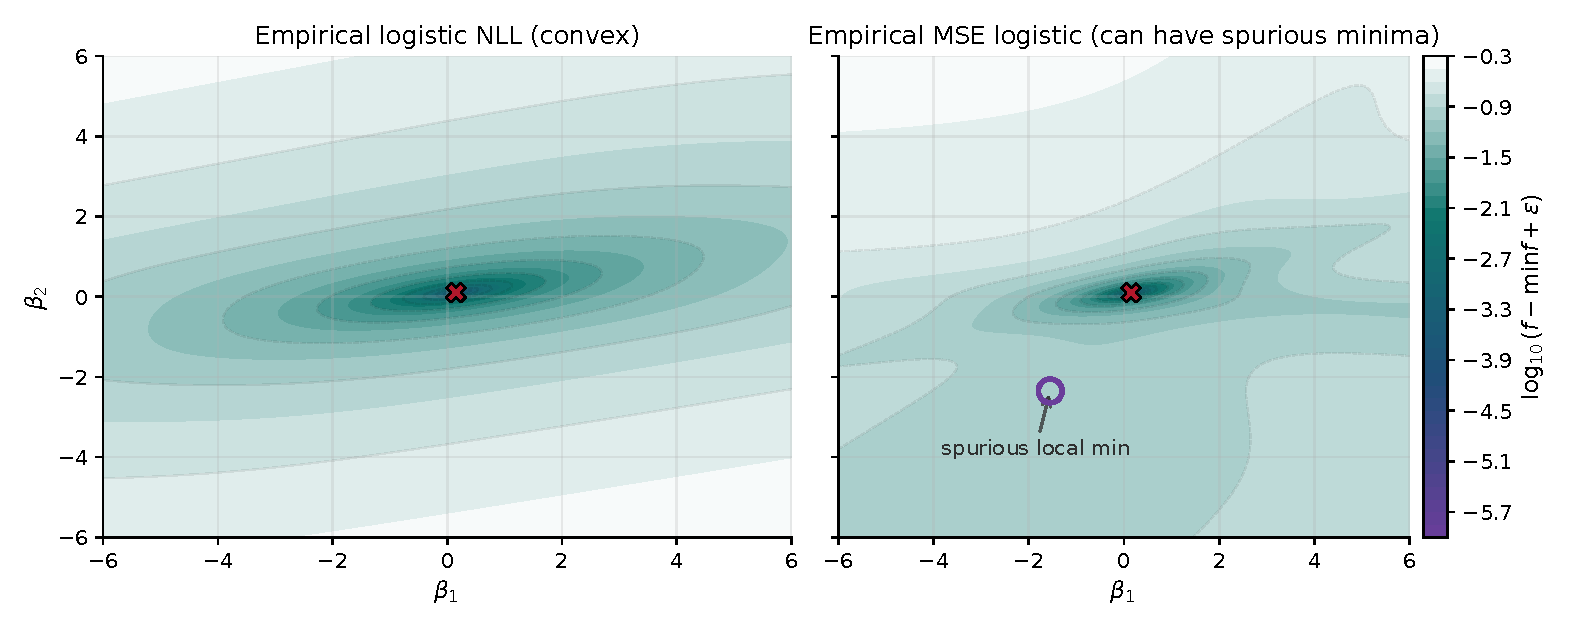
\includegraphics[width=\textwidth]{figures/handouts/convexity_optimization/fig_logistic_empirical_spurious}
  \caption{Empirical logistic landscapes on the dataset in \Cref{ex:logistic-empirical-spurious}.
  The plots show $\log_{10}(f-\min f+\varepsilon)$ for each objective.
  The red X marks the global minimizer in each panel.
  Left: the NLL is convex (one basin).
  Right: the squared-loss objective can have a spurious local minimum (circled), so a local method can get stuck.}
  \label{fig:logistic-empirical-spurious}
\end{figure}

\begin{figure}[t]
  \centering
  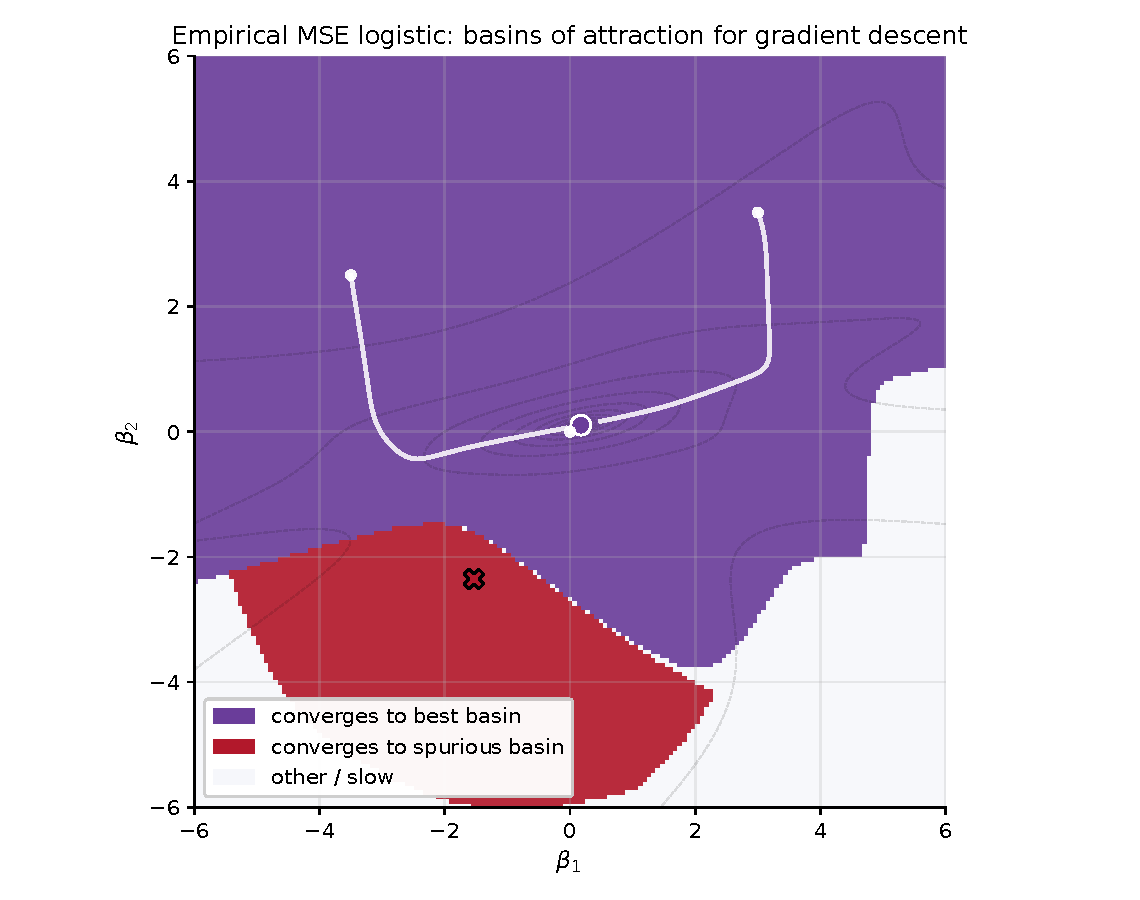
\includegraphics[width=0.92\textwidth]{figures/handouts/convexity_optimization/fig_logistic_empirical_basins}
  \caption{Basins of attraction for gradient descent on the empirical MSE-logistic objective in \Cref{ex:logistic-empirical-spurious}.
  The purple dot and red X mark the two local minimizers.
  Each initialization is colored by which local minimizer fixed-step GD (with $\eta=0.6$) converges to, and the overlaid paths show a few representative trajectories.}
  \label{fig:logistic-empirical-basins}
\end{figure}

Now assume a realizable population model:
\[
Y\mid X=x \sim \mathrm{Bernoulli}(p^\star(x)),
\qquad
p^\star(x) = \sigma(x^\top\beta^\star).
\]
Then the expected squared loss decomposes as
\[
\E\big[(Y-\sigma(X^\top\beta))^2\mid X\big]
= p^\star(X)(1-p^\star(X)) + \big(p^\star(X)-\sigma(X^\top\beta)\big)^2,
\]
so (up to an additive constant) the population objective becomes
\begin{equation}
R(\beta) = \E\big[(\sigma(X^\top\beta)-\sigma(X^\top\beta^\star))^2\big].
\label{eq:logistic-pop-risk}
\end{equation}

\begin{proposition}[One-point monotonicity in the realizable population squared-loss risk]
\label{prop:logistic-pop-one-point}
Assume $\E[\norm{X}_2]<\infty$, and let $R$ be as in \eqref{eq:logistic-pop-risk}. Then for all $\beta$,
\begin{equation}
\ip{\nabla R(\beta)}{\beta-\beta^\star} \ge 0.
\label{eq:one-point}
\end{equation}
In particular, along any ray $\beta(t)=\beta^\star+t(\beta-\beta^\star)$, the function $t\mapsto R(\beta(t))$ is nondecreasing for $t\ge 0$.
\end{proposition}

The next exercise isolates the population monotonicity calculation; structurally it plays the same role as the first-order convexity arguments in the Optimization unit.
\begin{exercise}[One-point monotonicity for realizable MSE-logistic]
\label{ex:logistic-one-point}
Prove \Cref{prop:logistic-pop-one-point}.
Let $\eta=X^\top\beta$ and $\eta^\star=X^\top\beta^\star$.
\begin{enumerate}[leftmargin=*]
  \item Differentiate under the expectation in \eqref{eq:logistic-pop-risk} to show that
  \[
  \nabla R(\beta)
  =2\,\E\Big[(\sigma(\eta)-\sigma(\eta^\star))\,\sigma'(\eta)\,X\Big].
  \]
  \item Show that
  \[
  \ip{\nabla R(\beta)}{\beta-\beta^\star}
  =2\,\E\Big[\sigma'(\eta)\,(\sigma(\eta)-\sigma(\eta^\star))(\eta-\eta^\star)\Big],
  \]
  and conclude it is nonnegative using only that $\sigma$ is increasing and $\sigma'\ge 0$.
  \item Deduce the ray-monotonicity statement by differentiating $g(t)=R(\beta^\star+t(\beta-\beta^\star))$.
\end{enumerate}
\end{exercise}

\SolutionBox[14]{%
\emph{Part (1).}
Differentiate \eqref{eq:logistic-pop-risk} under the expectation:
\[
R(\beta)=\E\big[(\sigma(X^\top\beta)-\sigma(X^\top\beta^\star))^2\big].
\]
Using the chain rule, $\nabla_\beta\sigma(X^\top\beta)=\sigma'(X^\top\beta)\,X$, hence
\[
\nabla R(\beta)
=2\,\E\Big[(\sigma(\eta)-\sigma(\eta^\star))\,\sigma'(\eta)\,X\Big],
\qquad
\eta=X^\top\beta,\ \eta^\star=X^\top\beta^\star.
\]

\emph{Part (2).}
Take the inner product with $(\beta-\beta^\star)$ and use $\ip{X}{\beta-\beta^\star}=\eta-\eta^\star$:
\[
\ip{\nabla R(\beta)}{\beta-\beta^\star}
=2\,\E\Big[\sigma'(\eta)\,(\sigma(\eta)-\sigma(\eta^\star))(\eta-\eta^\star)\Big].
\]
Since $\sigma'(\eta)\ge 0$ and $\sigma$ is increasing, we have
$(\sigma(\eta)-\sigma(\eta^\star))(\eta-\eta^\star)\ge 0$ pointwise.
Therefore the integrand is pointwise nonnegative, and the expectation is nonnegative as claimed.

\emph{Part (3) (ray monotonicity).}
For the ray $\beta(t)=\beta^\star+t(\beta-\beta^\star)$, define $g(t)=R(\beta(t))$.
By the chain rule,
\[
g'(t)=\ip{\nabla R(\beta(t))}{\beta-\beta^\star}\ge 0,
\]
so $t\mapsto R(\beta(t))$ is nondecreasing for $t\ge 0$.
(The argument uses only that the link is increasing with nonnegative derivative, so it holds for any such link function.)%
}

\begin{corollary}[Realizable population MSE-logistic has no spurious local minima]
\label{cor:logistic-pop-no-spurious}
Under the assumptions of \Cref{prop:logistic-pop-one-point}, every local minimizer of the realizable population risk $R$ in \eqref{eq:logistic-pop-risk} is global.
If in addition $\E[XX^\top]\succ 0$, then the unique global minimizer is $\beta^\star$.
\end{corollary}

\begin{exercise}[Stationarity + one-point monotonicity $\Rightarrow$ no spurious local minima]
\label{ex:logistic-one-point-no-spurious}
Prove \Cref{cor:logistic-pop-no-spurious} from \Cref{prop:logistic-pop-one-point}.
\begin{enumerate}[leftmargin=*]
  \item Let $\bar\beta$ be a local minimizer. Since $R$ is differentiable, $\nabla R(\bar\beta)=0$.
  Combine this with \Cref{eq:one-point} to show that
  \[
    0
    = \ip{\nabla R(\bar\beta)}{\bar\beta-\beta^\star}
    = 2\,\E\Big[\sigma'(\bar\eta)\,(\sigma(\bar\eta)-\sigma(\eta^\star))(\bar\eta-\eta^\star)\Big],
  \]
  where $\bar\eta=X^\top\bar\beta$ and $\eta^\star=X^\top\beta^\star$.
  Conclude that $\sigma(X^\top\bar\beta)=\sigma(X^\top\beta^\star)$ almost surely.
  \item Deduce that $R(\bar\beta)=0$, so $\bar\beta$ is a global minimizer.
  \item For uniqueness: show that if $R(\beta)=0$, then $X^\top(\beta-\beta^\star)=0$ almost surely, and deduce $\beta=\beta^\star$ under $\E[XX^\top]\succ 0$.
\end{enumerate}
\end{exercise}

\SolutionBox[14]{%
\emph{Part (1).}
Let $\bar\beta$ be a local minimizer of the differentiable function $R$.
Then $\nabla R(\bar\beta)=0$.
Applying \Cref{prop:logistic-pop-one-point} at $\beta=\bar\beta$ gives
\[
0
= \ip{\nabla R(\bar\beta)}{\bar\beta-\beta^\star}
= 2\,\E\Big[\sigma'(\bar\eta)\,(\sigma(\bar\eta)-\sigma(\eta^\star))(\bar\eta-\eta^\star)\Big],
\qquad \bar\eta=X^\top\bar\beta,\ \eta^\star=X^\top\beta^\star.
\]
The integrand is pointwise nonnegative because $\sigma'(\bar\eta)\ge 0$ and $\sigma$ is increasing, so the expectation can vanish only if the integrand is zero almost surely.
Since $\sigma'(z)>0$ for every finite $z$, this implies
\[
(\sigma(\bar\eta)-\sigma(\eta^\star))(\bar\eta-\eta^\star)=0
\qquad\text{almost surely.}
\]
Because $\sigma$ is strictly increasing, the product above is zero if and only if $\bar\eta=\eta^\star$, equivalently $\sigma(X^\top\bar\beta)=\sigma(X^\top\beta^\star)$ almost surely.

\emph{Part (2).}
If $\sigma(X^\top\bar\beta)=\sigma(X^\top\beta^\star)$ almost surely, then the integrand in \eqref{eq:logistic-pop-risk} vanishes almost surely, so
\[
R(\bar\beta)=\E\big[(\sigma(X^\top\bar\beta)-\sigma(X^\top\beta^\star))^2\big]=0.
\]
Since $R(\beta^\star)=0$ as well, $\bar\beta$ is a global minimizer.

\emph{Part (3) (uniqueness).}
If $R(\beta)=0$, then
\[
\E\big[(\sigma(X^\top\beta)-\sigma(X^\top\beta^\star))^2\big]=0,
\]
so $\sigma(X^\top\beta)=\sigma(X^\top\beta^\star)$ almost surely.
Since $\sigma$ is strictly increasing, this implies $X^\top(\beta-\beta^\star)=0$ almost surely.
Taking expectations yields
$(\beta-\beta^\star)^\top\E[XX^\top](\beta-\beta^\star)=0$.
If $\E[XX^\top]\succ 0$, then the quadratic form is strictly positive unless $\beta=\beta^\star$, so $\beta^\star$ is the unique global minimizer.%
}

The population MSE-logistic risk is nonconvex, but it still has the simple geometry that moving away from $\beta^\star$ does not help along any ray from $\beta^\star$.
This is qualitatively different from objectives like ecological logistic regression (\Cref{sec:ecological-logistic}), where aggregation introduces intrinsic nonconvexity and the landscape can have many distinct basins even under a clean population model.

Even with this benign global geometry, gradient descent can be slow because of saturation and flat plateaus.
The one-point monotonicity in \Cref{prop:logistic-pop-one-point} is a global geometry guarantee, but it is not a rate guarantee.
Far from $\beta^\star$, the squared-loss logistic objective can become very flat because the logistic link saturates:
$\sigma(z)\to 0$ or $1$ and $\sigma'(z)\to 0$ as $|z|\to\infty$.
The squared-loss gradient carries a factor of $\sigma'(X^\top\beta)$, so when the model is very confident (large $|X^\top\beta|$), the gradient can be tiny even if the objective value is not close to its minimum.
This mirrors the ``confidence weights'' story for convex NLL objectives:
in logistic NLL, curvature is largest near the decision boundary, while very confident points contribute little.
For squared loss, that same saturation suppresses the \emph{descent signal} itself, producing plateaus where $\norm{\nabla R(\beta)}_2$ is small even though $R(\beta)-R(\beta^\star)$ is not.

\begin{proposition}[Realizable squared-loss logistic: arbitrarily flat far from $\beta^\star$]
\label{prop:logistic-pop-flat}
Assume $\E[\norm{X}_2]<\infty$ and let $R$ be the realizable population risk \eqref{eq:logistic-pop-risk}.
Define $g(t)=R(t\beta^\star)$ for $t\ge 1$.
Then:
\begin{enumerate}[leftmargin=*]
  \item $g$ is nondecreasing on $[1,\infty)$ and converges to a finite limit $g(\infty)$.
  \item $\lim_{t\to\infty} g'(t)=0$ and $\lim_{t\to\infty}\norm{\nabla R(t\beta^\star)}_2=0$.
  \item If $\Pr(X^\top\beta^\star\neq 0)>0$, then $g(\infty)>0$.
\end{enumerate}
In particular, there are directions along which the landscape becomes arbitrarily flat even though the excess risk stays bounded away from $0$.
\end{proposition}

\emph{Proof idea.} See Exercise~\ref{ex:logistic-plateau}.

\begin{exercise}[Prove the plateau]
\label{ex:logistic-plateau}
In the realizable population model, let $g(t)=R(t\beta^\star)$ for $t\ge 1$.
\begin{enumerate}[leftmargin=*]
  \item Show that
  \[
    g'(t)=2\,\E\big[(\sigma(t\eta^\star)-\sigma(\eta^\star))\,\sigma'(t\eta^\star)\,\eta^\star\big],
    \qquad \eta^\star=X^\top\beta^\star,
  \]
  and conclude that $g$ is nondecreasing (hence $g(t)\to g(\infty)$ since $0\le g(t)\le 1$).
  \item Show that $g'(t)\to 0$ and $\nabla R(t\beta^\star)\to 0$ as $t\to\infty$.
  Interpret this as: \emph{without} a PL/strong-convexity-type condition, small gradient does not imply near-optimality.
  \item Assume $\Pr(\eta^\star\neq 0)>0$.
  Show that $g(\infty)>0$.
\end{enumerate}
\end{exercise}

\SolutionBox[12]{%
Write $\eta^\star=X^\top\beta^\star$ so that $g(t)=\E[(\sigma(t\eta^\star)-\sigma(\eta^\star))^2]$.

\emph{Part (1).}
Differentiate under the expectation:
by the chain rule,
\[
\frac{d}{dt}\sigma(t\eta^\star)=\sigma'(t\eta^\star)\,\eta^\star,
\]
so
\[
g'(t)
=\E\Big[2(\sigma(t\eta^\star)-\sigma(\eta^\star))\cdot \sigma'(t\eta^\star)\,\eta^\star\Big]
=2\,\E\big[(\sigma(t\eta^\star)-\sigma(\eta^\star))\,\sigma'(t\eta^\star)\,\eta^\star\big].
\]
For $t\ge 1$, $\sigma(t\eta^\star)-\sigma(\eta^\star)$ has the same sign as $(t-1)\eta^\star$ since $\sigma$ is increasing.
Because $\sigma'\ge 0$, the integrand is pointwise nonnegative, hence $g'(t)\ge 0$ and $g$ is nondecreasing.
Since $g(t)\in[0,1]$, it follows that $g(t)\to g(\infty)$ for some finite limit $g(\infty)$.

\emph{Part (2).}
For each fixed $\eta^\star\neq 0$, we have $t\eta^\star\to \pm\infty$ and therefore $\sigma'(t\eta^\star)\to 0$ as $t\to\infty$.
Also,
\[
\big|(\sigma(t\eta^\star)-\sigma(\eta^\star))\,\sigma'(t\eta^\star)\,\eta^\star\big|
\le \sigma'(0)\,|\eta^\star|
\le \sigma'(0)\,\norm{\beta^\star}_2\,\norm{X}_2,
\]
which is integrable since $\E[\norm{X}_2]<\infty$.
We will use the following standard fact: if random variables $Z_t$ satisfy $|Z_t|\le W$ with $\E[W]<\infty$ and $Z_t\to 0$ almost surely, then $\E[Z_t]\to 0$.
Applying this fact here gives $g'(t)\to 0$ as $t\to\infty$.

\smallskip
Similarly, differentiating \eqref{eq:logistic-pop-risk} gives
\[
\nabla R(t\beta^\star)
=2\,\E\big[(\sigma(t\eta^\star)-\sigma(\eta^\star))\,\sigma'(t\eta^\star)\,X\big].
\]
The integrand norm is bounded by $2\sigma'(0)\norm{X}_2$, and for each fixed $X$ the factor $\sigma'(t\eta^\star)$ tends to $0$ (or the bracketed term vanishes when $\eta^\star=0$), so the same reasoning lets us pass the limit through the expectation and conclude $\nabla R(t\beta^\star)\to 0$.

\emph{Part (3).}
As $t\to\infty$ we have $\sigma(t\eta^\star)\to 1$ when $\eta^\star>0$, $\sigma(t\eta^\star)\to 0$ when $\eta^\star<0$, and $\sigma(t\eta^\star)=\sigma(\eta^\star)=1/2$ when $\eta^\star=0$.
Since $0\le (\sigma(t\eta^\star)-\sigma(\eta^\star))^2\le 1$, we can apply the same fact (with $W=1$) to pass the limit through the expectation and obtain
\[
g(\infty)=\E\Big[(1-\sigma(\eta^\star))^2\mathbf{1}\{\eta^\star>0\} + \sigma(\eta^\star)^2\mathbf{1}\{\eta^\star<0\}\Big].
\]
If $\Pr(\eta^\star\neq 0)>0$, then the integrand is strictly positive on $\{\eta^\star\neq 0\}$, so $g(\infty)>0$.

Along this ray, the risk can remain bounded away from $0$ while the gradient (and directional derivative) goes to $0$.
Without a condition like PL/strong convexity, a small gradient does not by itself certify near-optimality.
}

Conditions like strong convexity or the PL inequality (\Cref{def:pl-inequality}) prevent this phenomenon: they rule out large flat regions away from the optimum by relating gradient size to suboptimality.
\Cref{prop:logistic-pop-flat} shows the realizable squared-loss logistic risk does not have such a global guarantee in general.

In the realizable population model, the one-point monotonicity in \Cref{prop:logistic-pop-one-point} is a \emph{global} geometric statement.
To get an actual rate for gradient descent, we also need a \emph{local curvature} condition near $\beta^\star$.
One simple sufficient condition is bounded features, which implies local strong convexity (hence a linear rate) around the optimum.

\begin{proposition}[Local linear convergence of gradient descent near $\beta^\star$]
\label{prop:logistic-pop-local-rate}
Assume $\E[XX^\top]\succeq \lambda I_d$ and $\norm{X}_2\le R$ almost surely for some $\lambda,R>0$.
Then at $\beta^\star$,
\[
\Hess R(\beta^\star)\succeq m_0 I_d,
\qquad
m_0 = 2\,\sigma'(R\norm{\beta^\star}_2)^2\,\lambda,
\]
and there exist $r>0$ and constants $0<m\le L<\infty$ such that the population risk $R$ in \eqref{eq:logistic-pop-risk} is $m$-strongly convex and $L$-smooth on the ball $\{\beta:\ \norm{\beta-\beta^\star}_2\le r\}$.
Consequently, gradient descent with step size $1/L$ initialized in this ball satisfies
\[
R(\beta^{(k)})-R(\beta^\star)
\le \left(1-\frac{m}{L}\right)^k\bigl(R(\beta^{(0)})-R(\beta^\star)\bigr)
\qquad\text{(see \citealp[\S9.3]{boyd_vandenberghe_2004_convex}).}
\]
\end{proposition}

\begin{proof}
Differentiate \eqref{eq:logistic-pop-risk} twice.
At $\beta=\beta^\star$, the cross term vanishes and the Hessian simplifies to
\[
\Hess R(\beta^\star)=2\,\E\big[\sigma'(X^\top\beta^\star)^2\,XX^\top\big].
\]
Since $\norm{X^\top\beta^\star}\le \norm{X}_2\norm{\beta^\star}_2\le R\norm{\beta^\star}_2$ almost surely, we have
$\sigma'(X^\top\beta^\star)\ge \sigma'(R\norm{\beta^\star}_2)>0$ almost surely (since $\sigma'$ is even and decreases with $|z|$), hence
\[
\Hess R(\beta^\star)\succeq 2\,\sigma'(R\norm{\beta^\star}_2)^2\,\E[XX^\top]\succeq 2\,\sigma'(R\norm{\beta^\star}_2)^2\,\lambda I_d.
\]
This is the claimed bound with $m_0=2\,\sigma'(R\norm{\beta^\star}_2)^2\,\lambda$.
Because $R$ is twice continuously differentiable and $\norm{X}_2\le R$ almost surely, $\Hess R(\beta)$ varies continuously in $\beta$ and is bounded on compact sets.
Therefore, on a sufficiently small ball around $\beta^\star$, the Hessian is bounded below by (say) $\tfrac12 m_0 I_d$ and above by $L I_d$ for some finite $L$, which gives local strong convexity and smoothness.
The linear convergence rate for gradient descent on an $m$-strongly convex and $L$-smooth function is standard (cited above).
\end{proof}

Under misspecification, hard multimodality can return.
If $p^\star(x)$ is not representable as $\sigma(x^\top\beta)$ (e.g.\ marginalizing over latent classes can yield mixtures of logits), then \eqref{eq:one-point} need not hold, and the population squared-loss risk can become bimodal with spurious local minima.
Benign global geometry often hinges on model and data assumptions.
This is one reason MLE (convex NLL) is often more stable than squared-loss fitting in logistic-type binary regression models.

\begin{example}[Misspecification can create a spurious local minimum for squared-loss logistic regression]
\label{ex:logistic-misspecified-spurious}
Consider a 1D feature $X$ that takes values $\{-2,-1,1,2\}$ with equal probability, and parameterize $\beta=(\beta_0,\beta_1)$ so that $q_\beta(x)=\sigma(\beta_0+\beta_1 x)$.
Let the true conditional probabilities be
\[
p^\star(-2)=0.49,\quad p^\star(-1)=0.87,\quad p^\star(1)=0.92,\quad p^\star(2)=0.36.
\]
This $p^\star$ is not representable as $q_\beta$, since it is not monotone in $x$.

For the population squared-loss risk $R_{\mathrm{MSE}}(\beta)=\E[(q_\beta(X)-p^\star(X))^2]$, a direct evaluation shows two distinct basins:
numerically, evaluating $R_{\mathrm{MSE}}$ on a grid reveals a global minimizer and a spurious local minimizer.
See \Cref{fig:logistic-landscape-2d}.
\end{example}

\begin{figure}[t]
  \centering
  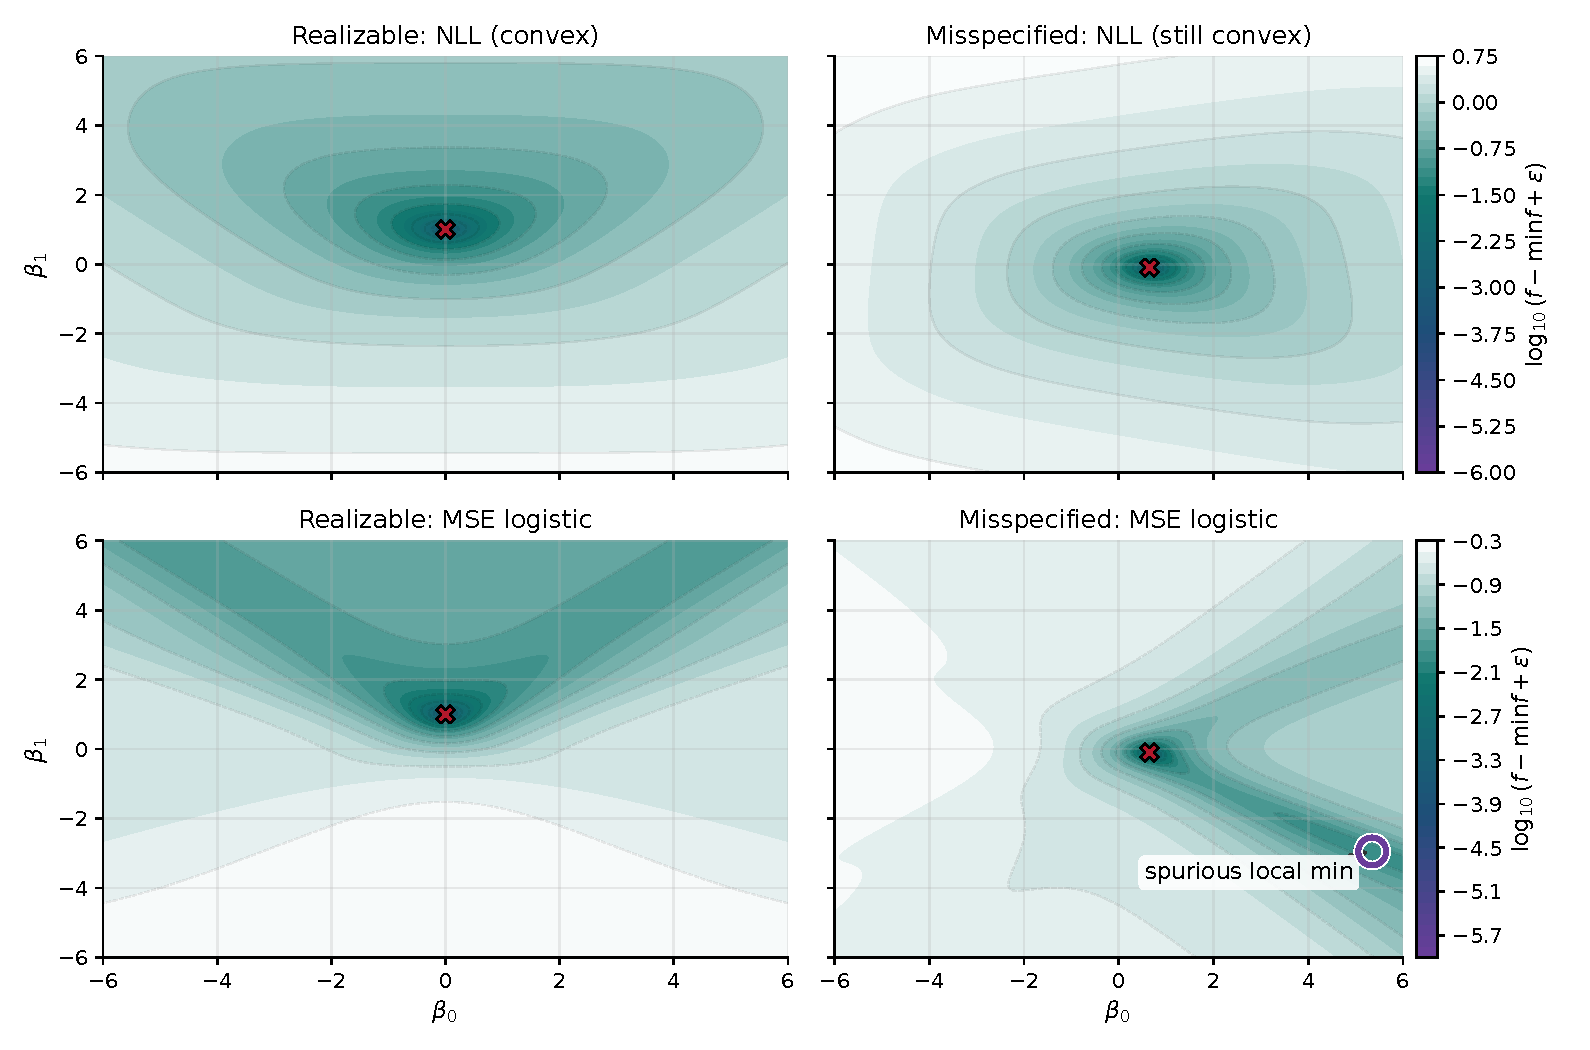
\includegraphics[width=\textwidth]{figures/handouts/convexity_optimization/fig_logistic_landscape_2d}
  \caption{A consistent contourf view of logistic landscapes in a 2D parameterization $\beta=(\beta_0,\beta_1)$.
  The plots show $\log_{10}(f-\min f+\varepsilon)$ for each objective, which makes basins comparable across panels.
  The red X marker indicates the global minimizer in each panel; in the bottom-right plot, the circled point is a spurious local minimum.
  In this example, the NLL landscape is unimodal in both realizable and misspecified settings, while the squared-loss landscape can develop extra basins under misspecification.}
  \label{fig:logistic-landscape-2d}
\end{figure}

% ------------------------------------------------------------
Example~I separates three distinct regimes.
Empirical MSE-logistic can create spurious basins; the realizable population risk has no spurious local minima but can still be slow because of broad plateaus; and misspecification can bring back genuinely wrong stable basins.
The response depends on the regime: use a stable objective when possible, use damping or line search when curvature is unreliable, and use restarts or stronger initializations when multiple basins are present.

% ------------------------------------------------------------
\section[Example II (phase retrieval)]{Example II: multimodality from symmetry, but only global optima in phase retrieval}
\label{sec:phase-retrieval}

In coherent diffraction imaging, optics, and astronomy, sensors measure intensities and lose phase.
A canonical real model is \emph{phase retrieval}:
\[
y_i = (a_i^\top x^\star)^2,\qquad i=1,\dots,m,
\]
where $x^\star\in\R^d$ is the unknown signal and $a_i$ are known sensing vectors.
A standard nonconvex least-squares objective is
\begin{equation}
F(x)=\frac{1}{4m}\sum_{i=1}^m\big((a_i^\top x)^2 - y_i\big)^2.
\label{eq:phase-empirical}
\end{equation}
This objective is nonconvex for structural reasons (it involves squares of linear forms),
and it is \emph{inherently} multimodal because $x^\star$ and $-x^\star$ generate the same data.

Like squared-loss logistic regression, phase retrieval is a smooth, nonconvex least-squares objective.
But here the nonconvexity is driven primarily by a \emph{symmetry}: $x^\star$ and $-x^\star$ generate the same data.
In population (for Gaussian designs), this symmetry produces multiple global optima but \emph{no} suboptimal local minima; the remaining stationary points are saddles.
This is ``benign'' nonconvexity (a strict-saddle picture), and it contrasts with ecological logistic regression (\Cref{sec:ecological-logistic}), where aggregation creates intrinsic nonconvexity and can lead to many distinct basins.
This ``benign geometry'' picture (multiple equivalent global minimizers; strict saddles elsewhere) appears broadly in modern tractable nonconvex problems; see \citet[\S2]{sun_qu_wright_2015_nonconvex_not_scary} and \citet[\S1]{zhang_qu_wright_2020_symmetry_geometry}.

\begin{figure}[t]
  \centering
  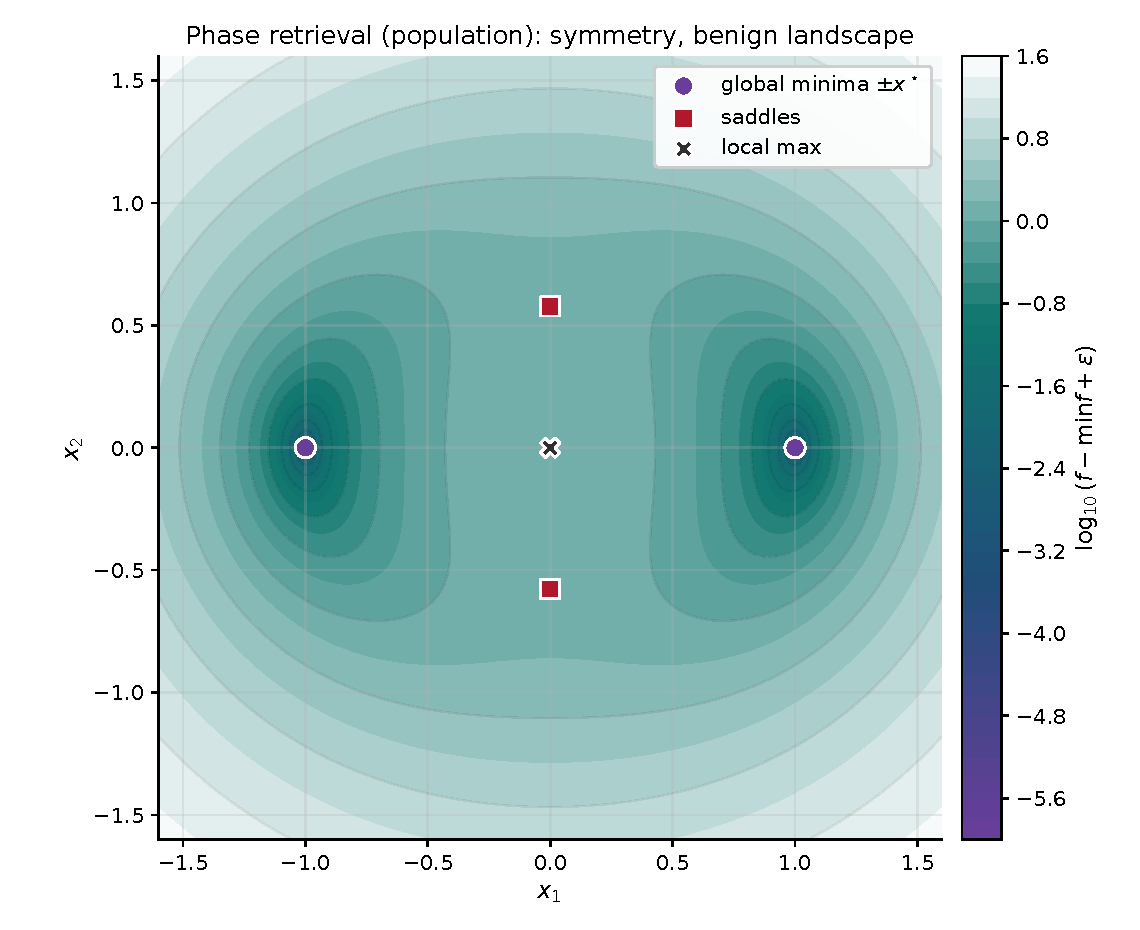
\includegraphics[width=0.86\textwidth]{figures/handouts/convexity_optimization/fig_phase_retrieval_landscape}
  \caption{Population phase retrieval in $d=2$: the landscape is nonconvex and symmetric ($x\sim -x$), but the only local minima are the two global minima $\pm x^\star$; other critical points are saddles or a local maximum at the origin.}
  \label{fig:phase-retrieval-landscape}
\end{figure}

For a clean population model, assume $a\sim N(0,I_d)$ and consider the \emph{population} objective
\begin{equation}
  f(x)=\frac12\,\E\Big[\big((a^\top x)^2 - (a^\top x^\star)^2\big)^2\Big].
  \label{eq:phase-pop}
\end{equation}

\begin{proposition}[Population phase retrieval: nonconvex but no spurious local minima]
\label{prop:phase-retrieval-benign}
For $f$ in \eqref{eq:phase-pop},
\begin{equation}
  f(x)
  =\frac{3}{2}\norm{x}^4 - \norm{x}^2\norm{x^\star}^2 - 2\ip{x}{x^\star}^2 + \frac{3}{2}\norm{x^\star}^4,
  \label{eq:phase-pop-closed-form}
\end{equation}
and the stationary points are:
\begin{enumerate}[leftmargin=*]
  \item global minima $x=\pm x^\star$ (value $0$),
  \item a local maximum at $x=0$,
  \item a saddle set $\{x:\ x\perp x^\star,\ \norm{x}=\norm{x^\star}/\sqrt{3}\}$.
\end{enumerate}
In particular, every local minimum is global.
\end{proposition}

\begin{exercise}[Phase retrieval: derive and classify the population stationary points]
\label{ex:phase-pop-derivation}
Prove \Cref{prop:phase-retrieval-benign}.
\begin{enumerate}[leftmargin=*]
  \item Expand \eqref{eq:phase-pop} and use the Gaussian fourth-moment identities
  \[
  \E[(a^\top u)^4]=3\norm{u}^4,
  \qquad
  \E[(a^\top u)^2(a^\top v)^2]=\norm{u}^2\norm{v}^2 + 2\ip{u}{v}^2,
  \]
  to obtain \eqref{eq:phase-pop-closed-form}.
  \item Differentiate \eqref{eq:phase-pop-closed-form} to get an explicit formula for $\nabla f(x)$.
  \item Solve $\nabla f(x)=0$ by decomposing $x=\alpha x^\star + u$ with $u\perp x^\star$.
  \item Classify the stationary points as global minima, a local maximum, and a saddle set.
\end{enumerate}
\end{exercise}

\SolutionBox[22]{%
\emph{Part (1) (closed form).}
Expanding the square in \eqref{eq:phase-pop} gives
\[
f(x)
=\frac12\,\E\big[(a^\top x)^4\big]
\;-\;\E\big[(a^\top x)^2(a^\top x^\star)^2\big]
\;+\;\frac12\,\E\big[(a^\top x^\star)^4\big].
\]
Apply the stated Gaussian fourth-moment identities with $u=x$ and $v=x^\star$ to get
\[
\E[(a^\top x)^4]=3\norm{x}^4,\qquad
\E[(a^\top x^\star)^4]=3\norm{x^\star}^4,
\]
and
\[
\E[(a^\top x)^2(a^\top x^\star)^2]=\norm{x}^2\norm{x^\star}^2 + 2\ip{x}{x^\star}^2.
\]
Substituting yields \eqref{eq:phase-pop-closed-form}.

\emph{Part (2) (gradient).}
Differentiate \eqref{eq:phase-pop-closed-form}:
\[
\nabla f(x)
= 6\norm{x}^2 x - 2\norm{x^\star}^2 x - 4\ip{x}{x^\star}x^\star
= (6\norm{x}^2-2\norm{x^\star}^2)x - 4\ip{x}{x^\star}x^\star.
\]

\emph{Part (3) (stationary points).}
Let $r=\norm{x^\star}_2$ and decompose $x=\alpha x^\star + u$ with $u\perp x^\star$.
Then $\ip{x}{x^\star}=\alpha r^2$ and $\norm{x}^2=\alpha^2r^2+\norm{u}^2$.
Setting $\nabla f(x)=0$ and matching the $u$ and $x^\star$ components gives
\[
(6\norm{x}^2-2r^2)\,u=0,
\qquad
\alpha\,(6\norm{x}^2-6r^2)=0.
\]
If $u=0$, then either $\alpha=0$ (so $x=0$) or $\norm{x}^2=r^2$ (so $\alpha=\pm 1$ and $x=\pm x^\star$).
If $u\neq 0$, then the first equation forces $\norm{x}^2=r^2/3$, and the second forces $\alpha=0$, hence
$x\perp x^\star$ and $\norm{x}=r/\sqrt{3}$.
This gives exactly the stationary-point list in \Cref{prop:phase-retrieval-benign}.

\emph{Part (4) (classification).}
Since $f$ in \eqref{eq:phase-pop} is an expectation of a square, $f(x)\ge 0$ for all $x$.
Also $f(\pm x^\star)=0$, so $\pm x^\star$ are global minima.

For $x=0$, the expansion \eqref{eq:phase-pop-closed-form} shows
\[
f(0)-f(x)= r^2\norm{x}^2 + 2\ip{x}{x^\star}^2 - \frac{3}{2}\norm{x}^4,
\]
which is strictly positive for all sufficiently small $x\neq 0$ (the quadratic term dominates), so $x=0$ is a local maximum.

Finally, if $x\perp x^\star$ and $\norm{x}=r/\sqrt{3}$, then the univariate restriction $t\mapsto f(x+t x^\star)$ has negative second derivative at $t=0$, so there is a direction of negative curvature.
Hence these points are saddles, and every local minimum is global.%
}

This is symmetry-driven nonconvexity with a strict-saddle geometry:
every non-optimal stationary point has a direction of negative curvature.

Phase retrieval is typically approached via the two-stage template in \Cref{alg:two-stage-template}:
use a cheap global initializer, then run a local method.
In the Gaussian model, there is a clean way to build a provably good direction estimate from a simple moment identity.
Assume the noiseless Gaussian design model $a_i \stackrel{\mathrm{iid}}{\sim} N(0,I_d)$ with measurements $y_i=(a_i^\top x^\star)^2$.
Define the \emph{spectral matrix}
\[
  Y = \frac{1}{m}\sum_{i=1}^m y_i a_i a_i^\top.
\]
Also define the radius estimate
\[
  \hat r^2 = \frac{1}{m}\sum_{i=1}^m y_i,
\]
which satisfies $\E[\hat r^2]=\norm{x^\star}_2^2$.
If $\hat u$ is a unit-norm top eigenvector of $Y$, then the standard spectral initializer is $x^{(0)}=\hat r\,\hat u$.

The next proposition explains why this initialization is reasonable.
It shows that (i) the population matrix $\E[Y]$ has a unique leading eigenvector in the $x^\star$ direction, and (ii) if the empirical $Y$ is close to $\E[Y]$ in operator norm then its leading eigenvector must be close to $\pm x^\star/\norm{x^\star}_2$.
(Here $\norm{M}_{\mathrm{op}}$ denotes the operator norm, i.e.\ the largest absolute eigenvalue for a symmetric matrix $M$.)

\begin{proposition}[Gaussian phase retrieval: why the spectral initializer points at $x^\star$]
\label{prop:phase-spectral-init}
Assume $x^\star\neq 0$, let $a\sim N(0,I_d)$, and set $y=(a^\top x^\star)^2$.
Write $r=\norm{x^\star}_2$ and $u^\star=x^\star/r$.
Define the population matrix
\[
  Y_{\mathrm{pop}} = \E\big[y\,a a^\top\big]
  = \E\big[(a^\top x^\star)^2 a a^\top\big].
\]
Then
\[
  Y_{\mathrm{pop}}=r^2 I_d + 2x^\star(x^\star)^\top,
\]
so the unique leading eigenvector of $Y_{\mathrm{pop}}$ is $u^\star$.
Moreover, if $Y$ is any symmetric matrix satisfying
\[
\norm{Y-Y_{\mathrm{pop}}}_{\mathrm{op}} \le \varepsilon\, r^2
\qquad\text{for some }\varepsilon\in(0,1),
\]
then for every unit-norm leading eigenvector $\hat u$ of $Y$ there exists a sign $s\in\{\pm 1\}$ such that
$\norm{\hat u-su^\star}_2\le \sqrt{2\varepsilon}$.
\end{proposition}

\begin{exercise}[Phase retrieval: why spectral initialization points at $x^\star$]
\label{ex:phase-spectral-spike}
Prove \Cref{prop:phase-spectral-init}.
Conclude that if the empirical matrix $Y$ is close to $Y_{\mathrm{pop}}$ in operator norm, then its top eigenvector is close to $\pm u^\star$ and the spectral initializer $x^{(0)}=\hat r\,\hat u$ is close to $\pm x^\star$.
\emph{Hint:} to compute $Y_{\mathrm{pop}}$, you can either compute entries using the Gaussian fourth-moment identity
$\E[a_i a_j a_k a_\ell]=\delta_{ij}\delta_{k\ell}+\delta_{ik}\delta_{j\ell}+\delta_{i\ell}\delta_{jk}$,
or compute the entries directly by expanding.
For the perturbation bound, compare quadratic forms $v^\top Y v$ and use $|v^\top (Y-Y_{\mathrm{pop}}) v|\le \norm{Y-Y_{\mathrm{pop}}}_{\mathrm{op}}$ for unit $v$.
Finally, explain in a sentence why one expects $\norm{Y-Y_{\mathrm{pop}}}_{\mathrm{op}}$ to be small when $m$ is large in the Gaussian model.
\end{exercise}

\SolutionBox[20]{%
Write $u=x^\star$ and expand $y=(a^\top u)^2=\sum_{k,\ell} u_k u_\ell a_k a_\ell$.
For each entry $(i,j)$,
\[
\E\!\big[y\,a_i a_j\big]
=\sum_{k,\ell} u_k u_\ell\,\E[a_i a_j a_k a_\ell]
=\sum_{k,\ell} u_k u_\ell\bigl(\delta_{ij}\delta_{k\ell}+\delta_{ik}\delta_{j\ell}+\delta_{i\ell}\delta_{jk}\bigr).
\]
The first term gives $\delta_{ij}\sum_k u_k^2=\delta_{ij}\norm{u}_2^2$.
The second and third terms each give $u_i u_j$.
Thus $\E[y\,a_i a_j]=\norm{u}_2^2\,\delta_{ij}+2u_i u_j$, i.e.
$Y_{\mathrm{pop}}=\norm{u}_2^2 I_d + 2uu^\top$.

For eigenvalues, note that $Y_{\mathrm{pop}}u=(\norm{u}_2^2+2\norm{u}_2^2)u=3\norm{u}_2^2 u$.
If $w\perp u$, then $uu^\top w=0$ so $Y_{\mathrm{pop}}w=\norm{u}_2^2 w$.
Hence the unique top eigenspace is $\mathrm{span}\{u\}$.

Let $r=\norm{u}_2$ and $u^\star=u/r$.
Let $\hat u$ be a unit top eigenvector of $Y$.
Write $E=Y-Y_{\mathrm{pop}}$ and assume $\norm{E}_{\mathrm{op}}\le \varepsilon r^2$.
Then
\[
\hat u^\top Y_{\mathrm{pop}} \hat u
= \hat u^\top Y \hat u - \hat u^\top E \hat u
\ge \lambda_{\max}(Y) - \norm{E}_{\mathrm{op}}
\ge (u^\star)^\top Y u^\star - \norm{E}_{\mathrm{op}}
\ge 3r^2 - 2\varepsilon r^2.
\]
On the other hand,
$
\hat u^\top Y_{\mathrm{pop}} \hat u
= r^2 + 2r^2\,|\ip{\hat u}{u^\star}|^2.
$
Combining gives $|\ip{\hat u}{u^\star}|^2\ge 1-\varepsilon$.
Choosing the sign that maximizes the inner product,
\[
\min\{\norm{\hat u-u^\star}_2,\norm{\hat u+u^\star}_2\}^2
=2\bigl(1-|\ip{\hat u}{u^\star}|\bigr)
\le 2\bigl(1-|\ip{\hat u}{u^\star}|^2\bigr)
\le 2\varepsilon.
\]

The matrix $Y$ is an empirical average of i.i.d.\ symmetric matrices with mean $Y_{\mathrm{pop}}$.
To make this quantitative in high dimensions, one uses concentration inequalities for random matrices to bound $\norm{Y-Y_{\mathrm{pop}}}_{\mathrm{op}}$ with high probability; see \citet[\S2.2]{zhang_qu_wright_2020_symmetry_geometry} for discussion and references.
These probability tools are largely orthogonal to our focus here.%
}

Once you have an initialization that is close to $\pm x^\star$, the local stage behaves like the convex story again.
In the Gaussian population objective, $\pm x^\star$ are not only global minima: they are \emph{locally strongly convex} minima, so the standard local strong-convexity analysis from the Optimization unit gives a linear rate while the iterates remain in that neighborhood.

\begin{exercise}[Phase retrieval: local convexity near $\pm x^\star$ in the population objective]
\label{ex:phase-pop-local-strong-convex}
For the population objective $f$ in \eqref{eq:phase-pop-closed-form}, compute the Hessian $\Hess f(x)$ and show that
\[
\Hess f(x^\star)=4\norm{x^\star}_2^2 I_d + 8x^\star(x^\star)^\top.
\]
Deduce the eigenvalues of $\Hess f(x^\star)$ and interpret this as a local condition-number statement near $x^\star$.
\end{exercise}

\SolutionBox[12]{%
Differentiate the gradient formula in the solution to \Cref{ex:phase-pop-derivation}:
for $x\in\R^d$,
\[
\Hess f(x)=12xx^\top + (6\norm{x}_2^2-2\norm{x^\star}_2^2)I_d - 4x^\star(x^\star)^\top.
\]
At $x=x^\star$ this becomes
\[
\Hess f(x^\star)=(12-4)x^\star(x^\star)^\top + 4\norm{x^\star}_2^2 I_d
=8x^\star(x^\star)^\top + 4\norm{x^\star}_2^2 I_d.
\]
Along $u^\star=x^\star/\norm{x^\star}_2$ the eigenvalue is $12\norm{x^\star}_2^2$, and along any direction orthogonal to $x^\star$ the eigenvalue is $4\norm{x^\star}_2^2$.
So near $x^\star$ the population objective is well conditioned (local condition number $3$), which is exactly the regime where local methods behave like in the convex case.%
}

These pieces give the standard Gaussian-model story:
spectral initialization supplies a direction close to $\pm x^\star$, and the local geometry near $\pm x^\star$ is strongly convex, so local methods converge quickly once initialized there.
Rigorous finite-sample analyses follow this template; see \citet[\S2.2]{zhang_qu_wright_2020_symmetry_geometry} and references therein.

Phase retrieval shows a different kind of nonconvexity.
The sign symmetry creates multiple optima, but they are equivalent, and the remaining stationary points are saddles rather than bad local minima.
The right response is therefore not exhaustive global search; it is a coarse initializer, such as a spectral method, followed by local refinement inside the basin of $\pm x^\star$.



% ------------------------------------------------------------
\section[Example III (ecological logistic)]{Example III: hard nonconvexity from aggregation in ecological logistic regression}
\label{sec:ecological-logistic}

In some applications we observe covariates at the unit level but only aggregated outcomes.
For example, we might see covariates $x_{g,1},\dots,x_{g,n_g}$ for individuals in a group (a precinct, a cohort, a batch),
but instead of observing the binary outcomes $Y_{g,i}\in\{0,1\}$ we only observe the group total
\[
Z_g = \sum_{i=1}^{n_g} Y_{g,i}.
\]
Many different binary vectors $(Y_{g,1},\dots,Y_{g,n_g})$ can produce the same total $Z_g$, so the likelihood for $\beta$ must marginalize over a large discrete set of latent ``assignments.''

Assume a logistic model at the unit level:
\[
\Pr(Y_{g,i}=1\mid x_{g,i},\beta)=\sigma(x_{g,i}^\top\beta),
\qquad i=1,\dots,n_g,
\]
with conditional independence across $i$ given the covariates.
Write $p_{g,i}(\beta)=\sigma(x_{g,i}^\top\beta)$.
Then $Z_g$ is a sum of independent but non-identically distributed Bernoulli random variables (a Poisson--binomial model), and the marginal likelihood contains $\binom{n_g}{z_g}$ terms.
The resulting negative log-likelihood is typically nonconvex in $\beta$.
This combinatorial marginalization also creates a separate difficulty that is easy to miss if we focus only on the geometry:
when $n_g$ is large, the likelihood term $\Pr(Z_g=z_g\mid x_{g,1},\dots,x_{g,n_g},\beta)$ can be expensive to evaluate repeatedly inside an optimizer.
The naive computation is literally a sum over $\binom{n_g}{z_g}$ assignments (as in \Cref{ex:eco-logistic-nonconvex}), which is intractable for large groups.
This ``optimization + marginalization'' pattern is common in latent-variable models: hard landscapes and expensive objective evaluations can come together.

An empirical negative log-likelihood objective for $G$ independent groups is
\begin{equation}
  f(\beta)
  =
  -\frac{1}{G}\sum_{g=1}^G \log \Pr(Z_g=z_g \mid x_{g,1},\dots,x_{g,n_g},\beta).
  \label{eq:eco-logistic-obj}
\end{equation}
Two edge cases are instructive.
In the special case where the covariates are constant within each group ($x_{g,i}\equiv x_g$), we have
$Z_g\sim \mathrm{Binomial}(n_g,\sigma(x_g^\top\beta))$, and \eqref{eq:eco-logistic-obj} reduces to the usual convex binomial logistic-regression objective from the Optimization unit.
At the other extreme, if $d=1$ with $\beta=(\beta_0,\beta_1)$ and each group contains covariates in $\pm$ pairs (for every $x$ the value $-x$ appears with the same multiplicity), then the marginal likelihood is symmetric in the slope: it is unchanged under $\beta_1\mapsto -\beta_1$.
This kind of symmetry reflects a genuine non-identifiability from totals alone.

\begin{exercise}[Ecological logistic regression: two easy special cases]
\label{ex:eco-logistic-edge-cases}
\begin{enumerate}[leftmargin=*]
  \item Suppose $x_{g,i}\equiv x_g$ within each group.
  Show that $Z_g\sim \mathrm{Binomial}(n_g,\sigma(x_g^\top\beta))$ and conclude that the corresponding negative log-likelihood is convex in $\beta$.
  \item Assume $d=1$ with $\beta=(\beta_0,\beta_1)$ and suppose the multiset $\{x_1,\dots,x_n\}$ is symmetric: for every $x$ it contains $-x$ with the same multiplicity.
  Show that, for every $z$,
  \[
    \Pr(Z=z\mid x_1,\dots,x_n,(\beta_0,\beta_1))
    =
    \Pr(Z=z\mid x_1,\dots,x_n,(\beta_0,-\beta_1)).
  \]
  Conclude that the likelihood for $\beta_1$ is an even function, so the sign of the slope is not identifiable from $Z$ alone in such a balanced design.
\end{enumerate}
\end{exercise}

\SolutionBox[14]{%
\emph{Part (1).}
If $x_{g,i}\equiv x_g$, then conditional on $x_g$ the unit-level outcomes are i.i.d.\ Bernoulli with success probability $\sigma(x_g^\top\beta)$.
Therefore $Z_g=\sum_{i=1}^{n_g}Y_{g,i}\sim \mathrm{Binomial}(n_g,\sigma(x_g^\top\beta))$.
Up to an additive constant (independent of $\beta$), the per-group negative log-likelihood can be written as a function of the scalar $\eta=x_g^\top\beta$:
\[
\ell_g(\beta)
= -z_g\,\eta + n_g\log(1+e^\eta).
\]
Since $\frac{d^2}{d\eta^2}\ell_g(\eta)=n_g\,\sigma'(\eta)\ge 0$, the map $\eta\mapsto \ell_g(\eta)$ is convex.
Composing a convex function with a linear map $\beta\mapsto x_g^\top\beta$ preserves convexity, so $\ell_g$ is convex in $\beta$.
Summing over $g$ preserves convexity, hence the full objective is convex.

\emph{Part (2).}
Write $p_i(\beta_0,\beta_1)=\sigma(\beta_0+\beta_1 x_i)$.
Replacing $\beta_1$ by $-\beta_1$ replaces $p_i$ by $\tilde p_i=\sigma(\beta_0-\beta_1 x_i)$.
By the assumed symmetry of the multiset $\{x_i\}$, the multiset $\{\tilde p_i\}$ is the same as $\{p_i\}$ up to a permutation (each $x$ is paired with $-x$).
But the distribution of $Z=\sum_i Y_i$ depends only on the multiset of success probabilities, not on how they are ordered, so $\Pr(Z=z\mid x_1,\dots,x_n,(\beta_0,\beta_1))=\Pr(Z=z\mid x_1,\dots,x_n,(\beta_0,-\beta_1))$ for every $z$.
Thus the likelihood is an even function of $\beta_1$, which means the sign of the slope is not identifiable from totals in this balanced design.%
}

This example ties directly to the empirical-versus-population theme from Example~I.
There the bad basins can be a finite-sample artifact under benign population geometry; here the nonconvexity is intrinsic, because even under the correct model and infinite data aggregation forces us to marginalize over discrete latent assignments.
That marginalization step is also the bridge to the Expectation--maximization subsection of the Augmented-state optimization unit: once the assignments are latent, the natural algorithmic object is the EM update map, which alternates exact conditional expectations with parameter updates, rather than a single closed-form convex objective.

To emphasize this, it is useful to look at a \emph{population} version of \eqref{eq:eco-logistic-obj}.
Let $X=(x_1,\dots,x_n)$ denote a random group of covariates and let $Z$ be generated from the model under a true parameter $\beta^\star$.
Define the population objective
\[
F(\beta)=\E\big[-\log \Pr(Z\mid X,\beta)\big].
\]
Because the model is correctly specified, $F$ is minimized at (an observationally equivalent version of) $\beta^\star$.
However, as \Cref{fig:eco-logistic-pop-landscape} illustrates, $F$ can still have multiple separated basins and spurious local minima.

\begin{figure}[H]
  \centering
  \input{figures/handouts/convexity_optimization/fig_ecological_logistic_population_landscape}
  \caption{A toy \emph{population} objective for ecological logistic regression in a 2D parameterization $\beta=(\beta_0,\beta_1)$.
  Each group has $n=6$ units and is equally likely to have covariates $(-4,-3,-2,2,3,4)$, $(-3,-1,1,2,3,4)$, or $(-2,-1,1,2,3,4)$ (in $d=1$); outcomes are generated under $\beta^\star=(0.3,1.2)$.
  The plot shows $\log_{10}(F-\min F+\varepsilon)$, as in \Cref{fig:logistic-landscape-2d}; the red X marks $\beta^\star$ and the open circles mark three spurious local minima in this toy example.}
  \label{fig:eco-logistic-pop-landscape}
\end{figure}

\begin{exercise}[Ecological logistic regression: marginalization and nonconvexity]
\label{ex:eco-logistic-nonconvex}
Fix one group with covariates $x_1,\dots,x_n\in\R^d$ and observe $Z=z$.
Let $p_i(\beta)=\sigma(x_i^\top\beta)$.
\begin{enumerate}[leftmargin=*]
  \item Show that
  \[
    \Pr(Z=z\mid x_1,\dots,x_n,\beta)
    =
    \sum_{\substack{S\subseteq\{1,\dots,n\}\\|S|=z}}
    \ \prod_{i\in S} p_i(\beta)\prod_{j\notin S}\bigl(1-p_j(\beta)\bigr).
  \]
  Interpret this as summing over all ways to choose which $z$ units are the successes.
  \item Specialize to $n=2$ and $z=1$ in $d=1$ with covariates $x_1=a$ and $x_2=b$.
  Let $\ell(\beta)$ be the negative log-likelihood $-\log \Pr(Z=1\mid a,b,\beta)$ with no regularization.
  Show that $\ell''(0)=\tfrac12 ab$.
  Conclude that $\ell$ is not convex whenever $ab<0$.
\end{enumerate}
\end{exercise}

\SolutionBox[20]{%
\emph{Part (1).}
Condition on the covariates.
For any binary vector $y=(y_1,\dots,y_n)\in\{0,1\}^n$, conditional independence gives
\[
\Pr(Y_1=y_1,\dots,Y_n=y_n\mid x_1,\dots,x_n,\beta)
=
\prod_{i=1}^n p_i(\beta)^{y_i}\bigl(1-p_i(\beta)\bigr)^{1-y_i}.
\]
The event $\{Z=z\}$ is the union of all assignments $y$ with exactly $z$ ones, so summing over those assignments yields
\[
\Pr(Z=z\mid x_1,\dots,x_n,\beta)
=
\sum_{\substack{y\in\{0,1\}^n\\ \sum_i y_i=z}}
\ \prod_{i=1}^n p_i(\beta)^{y_i}\bigl(1-p_i(\beta)\bigr)^{1-y_i}.
\]
Reindexing the sum by the subset $S=\{i:\ y_i=1\}$ (which has $|S|=z$) gives the stated formula.

\emph{Part (2).}
For $n=2$ and $z=1$, let $p_1(\beta)=\sigma(a\beta)$ and $p_2(\beta)=\sigma(b\beta)$.
Then
\[
q(\beta)=\Pr(Z=1\mid a,b,\beta)
 = p_1(1-p_2) + (1-p_1)p_2
 = p_1+p_2-2p_1p_2,
\]
and $\ell(\beta)=-\log q(\beta)$.
At $\beta=0$ we have $p_1=p_2=\tfrac12$, so $q(0)=\tfrac12$.
Also $p_1'(\beta)=a\,p_1(1-p_1)$ and $p_2'(\beta)=b\,p_2(1-p_2)$, so $p_1'(0)=a/4$ and $p_2'(0)=b/4$.
A direct differentiation gives $q'(0)=0$ and
\[
q''(0)=-4p_1'(0)p_2'(0)=-4\cdot\frac{a}{4}\cdot\frac{b}{4}=-\frac{ab}{4}.
\]
Since $\ell'=-q'/q$ and $q'(0)=0$, we have $\ell''(0)=-(q''(0)/q(0))$ and therefore
\[
\ell''(0)
=-\frac{q''(0)}{q(0)}
=-\frac{-ab/4}{1/2}
=\frac{ab}{2}.
\]
If $ab<0$, then $\ell''(0)<0$, so $\ell$ is not convex.
}

Even though the landscape can be globally hard (and even the population objective can have spurious basins, as in \Cref{fig:eco-logistic-pop-landscape}), there is still a familiar ``convex'' story \emph{locally} around the true parameter under correct specification.
When the model is locally identifiable, the population objective has a neighborhood of $\beta^\star$ on which it is convex (indeed strongly convex).
One convenient way to see this in ecological logistic regression is to expose the probabilistic structure behind the gradient and Hessian: the observed-data objective involves marginalizing over latent assignments, and its Hessian can be written as a difference of two covariance matrices.
After averaging over the random total $Z$ under the true model, that difference becomes a covariance by the law of total covariance.

\begin{exercise}[Ecological logistic regression: DC structure and local convexity near $\beta^\star$]
\label{ex:eco-logistic-pop-local-convex}
Fix covariates $x_1,\dots,x_n\in\R^d$.
For $\beta\in\R^d$, let $V_1,\dots,V_n$ be independent Bernoulli random variables with
\[
\Pr(V_j=1\mid x_j,\beta)=\sigma(x_j^\top\beta),
\qquad j=1,\dots,n,
\]
and define
\[
U = \sum_{j=1}^n x_j V_j,
\qquad
Z = \sum_{j=1}^n V_j.
\]
For an observed total $Z=z$, write $L_z(\beta)=-\log \Pr(Z=z\mid x_1,\dots,x_n,\beta)$.
\begin{enumerate}[leftmargin=*]
  \item Show the \emph{difference-of-convex (DC)} form
  \[
  L_z(\beta)
  =\sum_{j=1}^n \log\bigl(1+e^{x_j^\top\beta}\bigr)
  -\log\left(\sum_{\substack{S\subseteq\{1,\dots,n\}\\|S|=z}} \exp\Big(\sum_{j\in S} x_j^\top\beta\Big)\right).
  \]
  \item Show that $\nabla L_z(\beta)=\E[U]-\E[U\mid Z=z]$.
  \item Show that $\Hess L_z(\beta)=\mathrm{Cov}(U)-\mathrm{Cov}(U\mid Z=z)$.
  (Hint: for $g(\beta)=\log\sum_k e^{a_k^\top\beta}$, the Hessian is the covariance of the vectors $\{a_k\}$ under the corresponding softmax weights.)
  \item Consider the population objective $F(\beta)=\E[L_Z(\beta)]$ when $Z$ is generated under a true parameter $\beta^\star$.
  Assuming the outer expectation defining $F$ can be differentiated twice under the integral sign, use the conditional law of total covariance,
  \[
    \mathrm{Cov}(U\mid X)=\E[\mathrm{Cov}(U\mid Z,X)\mid X] + \mathrm{Cov}(\E[U\mid Z,X]\mid X),
  \]
  to show that
  \[
    \E\big[\Hess L_Z(\beta^\star)\mid X\big]
    = \mathrm{Cov}\big(\E[U\mid Z,X]\mid X\big)\succeq 0.
  \]
  Deduce that
  \[
    \Hess F(\beta^\star)
    = \E\Big[\mathrm{Cov}\big(\E[U\mid Z,X]\mid X\big)\Big]\succeq 0.
  \]
  Conclude that if $\Hess F(\beta^\star)\succ 0$, then $F$ is locally strongly convex on a neighborhood of $\beta^\star$.
\end{enumerate}
\end{exercise}

\SolutionBox[22]{%
\emph{Part (1).}
Write $\eta_j=x_j^\top\beta$ and $p_j=\sigma(\eta_j)=e^{\eta_j}/(1+e^{\eta_j})$.
For any subset $S$ with $|S|=z$,
\[
\Pr(V_j=1\ \forall j\in S,\ V_j=0\ \forall j\notin S\mid x_1,\dots,x_n,\beta)
=\prod_{j\in S}p_j\prod_{j\notin S}(1-p_j)
=\frac{\exp(\sum_{j\in S}\eta_j)}{\prod_{j=1}^n(1+e^{\eta_j})}.
\]
Summing over all $S$ with $|S|=z$ gives
\[
\Pr(Z=z\mid x_1,\dots,x_n,\beta)
=\frac{\sum_{|S|=z}\exp(\sum_{j\in S}\eta_j)}{\prod_{j=1}^n(1+e^{\eta_j})}.
\]
Taking $-\log$ yields the stated DC representation.

\emph{Parts (2) and (3).}
The first term in $L_z$ has gradient $\sum_j \sigma(\eta_j)x_j$ and Hessian $\sum_j \sigma'(\eta_j)x_jx_j^\top$.
Since $U=\sum_j x_j V_j$ with independent Bernoulli coordinates, these are exactly $\E[U]$ and $\mathrm{Cov}(U)$.

For the second term, define a probability distribution on subsets $S$ of size $z$ by
\[
w_S(\beta)\propto \exp\Big(\sum_{j\in S}x_j^\top\beta\Big),
\qquad |S|=z.
\]
This is the conditional law of the success set $\{j:\ V_j=1\}$ given $Z=z$ under parameter $\beta$.
Therefore
\[
\nabla \log\Big(\sum_{|S|=z} e^{\sum_{j\in S}x_j^\top\beta}\Big)
  = \sum_{|S|=z} w_S(\beta)\sum_{j\in S}x_j
  = \E[U\mid Z=z],
\]
and differentiating once more gives
\[
\Hess\!\left(\log\Big(\sum_{|S|=z} e^{\sum_{j\in S}x_j^\top\beta}\Big)\right)
=\mathrm{Cov}(U\mid Z=z),
\]
which yields $\nabla L_z=\E[U]-\E[U\mid Z=z]$ and $\Hess L_z=\mathrm{Cov}(U)-\mathrm{Cov}(U\mid Z=z)$.

\emph{Part (4).}
Now let $X=(x_1,\dots,x_n)$ be random, and assume we may differentiate the outer expectation in $F(\beta)=\E[L_Z(\beta)]$ twice under the integral sign.
Conditional on $X$ and at $\beta^\star$, take expectations over $Z$:
\[
\E\big[\Hess L_Z(\beta^\star)\mid X\big]
=\mathrm{Cov}(U\mid X)-\E[\mathrm{Cov}(U\mid Z,X)\mid X].
\]
By the conditional law of total covariance,
\[
\mathrm{Cov}(U\mid X)
=\E[\mathrm{Cov}(U\mid Z,X)\mid X] + \mathrm{Cov}(\E[U\mid Z,X]\mid X),
\]
so the difference is
\[
\E\big[\Hess L_Z(\beta^\star)\mid X\big]
=\mathrm{Cov}(\E[U\mid Z,X]\mid X)\succeq 0.
\]
Taking outer expectations gives
\[
\Hess F(\beta^\star)
=\E\big[\Hess L_Z(\beta^\star)\big]
=\E\Big[\mathrm{Cov}(\E[U\mid Z,X]\mid X)\Big]\succeq 0.
\]
If this unconditional Hessian is positive definite, then by continuity of $\Hess F$ there exists a radius $r>0$ such that $\Hess F(\beta)\succeq \tfrac12 \Hess F(\beta^\star)\succ 0$ on $\{\beta:\ \norm{\beta-\beta^\star}_2\le r\}$, which implies local strong convexity of $F$ on that neighborhood.%
}

This example still fits the two-stage template in \Cref{alg:two-stage-template}, but the coarse stage is less structured.
In practice, one often uses multiple random starts or a warm start from a crude convex surrogate, then runs a local optimizer with line search or damping on the true nonconvex objective \eqref{eq:eco-logistic-obj} and keeps the best solution found.

Ecological logistic regression is the genuinely hard case in this note.
Aggregation forces a sum over latent assignments, so the objective can have many distinct basins even under correct specification.
The practical response is usually robust search rather than a single clever local method: several starts, warm starts from crude convex surrogates when available, and then local refinement with damping or line search on the true objective.



% ------------------------------------------------------------
\section{Diagnosing nonconvex objectives}
\label{sec:checklist-streamlined}

``Nonconvex'' is not a single regime.
Squared-loss logistic regression is close to convex: the empirical objective can have spurious minima, yet under realizability the population geometry is benign and locally strongly convex near $\beta^\star$.
Phase retrieval is symmetry-driven: there can be multiple equivalent optima but no bad local minima.
Ecological logistic regression is intrinsically hard because aggregation induces latent assignments and the resulting marginal likelihood can have many distinct basins.
The right response depends on which regime you are in: stable objectives when available, spectral or other coarse initialization when symmetry is the issue, and restarts or stronger surrogates when aggregation drives the hardness.
This is also the lens used in the Expectation--maximization subsection of the Augmented-state optimization unit: the basin picture remains central, but the relevant geometry is now the geometry of the EM operator and its population/sample perturbations.

A useful diagnosis is to ask whether the difficulty comes from finite-sample noise or the population model, from symmetry or non-identifiability, from genuinely suboptimal basins, from the lack of a global guarantee beyond convexity, or simply from poor local conditioning.
Carried back to the main notes, the point is not that nonconvexity is uniformly hopeless.
The real question is which part of the convex story breaks first: the basin structure, the conditioning inside a good basin, or only the finite-sample objective we happen to optimize.

\begin{table}[t]
  \centering
  \small
  \setlength{\tabcolsep}{4pt}
  \begin{tabular}{@{}p{0.18\textwidth}p{0.24\textwidth}p{0.26\textwidth}p{0.24\textwidth}@{}}
    \toprule
    Example & Source of nonconvexity & Global geometry & Typical response \\
    \midrule
    Logistic: NLL vs MSE & objective choice + assumptions & spurious basins can appear empirically/misspecified; realizable population is benign but can be flat & pick a stable objective (NLL), add damping/restarts, check misspecification \\
    Phase retrieval & symmetry ($x\sim -x$) & strict-saddle population landscape; only local minima are global & spectral init + local refinement; perturb/noise to escape saddles \\
    Ecological\newline logistic & aggregation / missing labels & many distinct basins from latent assignments & many restarts; warm starts; keep best \\
    \bottomrule
  \end{tabular}
  \caption{Summary of the three examples by source of nonconvexity, resulting global geometry, and typical response.
  Together the columns instantiate the ``hardness = basins + geometry'' spine developed in the handout.}
  \label{tab:nonconvex-example-summary}
\end{table}

\bibliographystyle{plainnat}
\makeatletter
\begingroup
\let\input@path\@empty
\IfFileExists{references.bib}{%
  \gdef\stat221bibpath{references}%
}{%
  \IfFileExists{../references.bib}{%
    \gdef\stat221bibpath{../references}%
  }{%
    \gdef\stat221bibpath{../../references}%
  }%
}
\endgroup
\makeatother
\bibliography{\stat221bibpath}

\end{document}
"
%   (Low-level direct build: if you invoke latexmk manually, set -jobname to the
%    titled output so the compiled PDF matches the standard naming scheme.)
%     (cd "Lecture Tex/handouts/section 1" && latexmk -pdf -interaction=nonstopmode -halt-on-error \
%       -pdflatex='pdflatex %O "\\def\\STATshowsolutions{1}\\input{%S}"' section_convexity_optimization.tex)
%   (If you prefer the legacy flag name with digits, use a csname:)
%     pdflatex "\expandafter\def\csname STAT221SOLUTIONS\endcsname{1}\documentclass[11pt]{article}

% Make this file compilable from the repo root or within `Lecture Tex/handouts/`.
\makeatletter
\def\input@path{{../../}{../}{Lecture Tex/}}
\makeatother
\input{preamble}
\usepackage{float} % for [H] placement specifier in algorithms

\graphicspath{{../../}{../}{Lecture Tex/}{../../figures/}{../figures/}{Lecture Tex/figures/}}

% ------------------------------------------------------------
% Build toggle for solutions.
% - Student version (default): show workspace boxes, hide solutions.
% - Solutions version: define \STATshowsolutions on the command line.
%   Preferred repo-level build (compiles the titled PDFs directly and clears legacy outputs):
%     python3 scripts/build_handouts.py --section 1
%   Example:
%     pdflatex "\def\STATshowsolutions{1}\input{Lecture Tex/handouts/section 1/section_convexity_optimization.tex}"
%   (Low-level direct build: if you invoke latexmk manually, set -jobname to the
%    titled output so the compiled PDF matches the standard naming scheme.)
%     (cd "Lecture Tex/handouts/section 1" && latexmk -pdf -interaction=nonstopmode -halt-on-error \
%       -pdflatex='pdflatex %O "\\def\\STATshowsolutions{1}\\input{%S}"' section_convexity_optimization.tex)
%   (If you prefer the legacy flag name with digits, use a csname:)
%     pdflatex "\expandafter\def\csname STAT221SOLUTIONS\endcsname{1}\input{Lecture Tex/handouts/section 1/section_convexity_optimization.tex}"
\newif\ifshowsolutions
\showsolutionsfalse
\ifdefined\STATshowsolutions
  \showsolutionstrue
\fi
\ifcsname STAT221SOLUTIONS\endcsname
  \showsolutionstrue
\fi

% Handout-only tcolorbox style for readable title bars.
% The `stat221titlebox` tcolorbox style is defined in `Lecture Tex/preamble.tex`.

% Solution boxes (controlled by \ifshowsolutions).
% Usage: \SolutionBox{<solution body>}
\newcommand{\SolutionBox}[2][10]{%
  \ifshowsolutions
    \begin{tcolorbox}[stat221panelgray,title={Solution}]
    #2
    \end{tcolorbox}
  \else
    \begin{tcolorbox}[stat221panelgray,unbreakable,title={Workspace}]
    \vspace{#1\baselineskip}
    \end{tcolorbox}
  \fi
}

\title{When does nonconvexity make optimization hard?}
\author{}
\date{}

\begin{document}
\maketitle

\section[Nonconvexity and optimization hardness]{When does nonconvexity make optimization hard?}
\label{sec:convexity-opt-hardness-handout}

Optimization in this course starts from minimizing smooth objectives with local information: gradients, Hessians, line searches, and condition numbers describe what a descent method can see near the current iterate.
This handout asks when that local picture ceases to be the whole story once the objective is no longer convex.
The main objects are the landscape itself, the basins created by that landscape, and the local geometry that determines how quickly a method moves within a basin.

That perspective builds directly on the Optimization unit and feeds forward to the Augmented-state optimization unit, where the same basin-versus-geometry split reappears for the EM update map rather than for a single objective.
Logistic regression, phase retrieval, and ecological logistic regression then supply three contrasting regimes: an objective choice that can create misleading empirical basins, a symmetry-driven landscape with multiple equivalent optima but no bad local minima, and an intrinsically hard latent-assignment problem.

% ------------------------------------------------------------
\section[Basins and geometry]{Basins, geometry, and what local methods can promise}
\label{sec:framing-nonconvex}

Nonconvex analysis in Stat~221 still starts from the same local-method toolkit as the convex case:
\emph{smoothness} gives a descent lemma, and \emph{curvature} controls local speed.
What changes is the global question of whether the landscape contains suboptimal basins that can trap a local method away from the best achievable value.

\begin{definition}[Basic vocabulary]
\label{def:basic-vocab-nonconvex}
Let $f:\R^d\to\R$ be differentiable and write $f^\star=\inf_x f(x)$.
\begin{enumerate}[leftmargin=*]
  \item A point $x$ is a \textbf{stationary point} if $\nabla f(x)=0$.
  \item A point $x$ is a \textbf{local minimizer} if $f(x)\le f(x')$ for all $x'$ in some neighborhood of $x$.
  A local minimizer is \textbf{spurious} if $f(x)>f^\star$.
  \item A \textbf{(strict) saddle} is a stationary point $x$ with a direction of negative curvature, i.e.\ there exists $v$ such that $v^\top \Hess f(x)\,v<0$.
  \item Fix an algorithm (e.g.\ gradient descent with a specified step-size rule).
  The \textbf{basin of attraction} of a limit point $\bar x$ is the set of initializations $x^{(0)}$ for which the iterates converge to $\bar x$.
  Basins depend on the method and its hyperparameters.
\end{enumerate}
\end{definition}

In practice, local methods succeed when descent is reliable, stationary points are safe, and the initialization lands in a basin where the local geometry is favorable.
Because this is a statistical optimization class, we will repeatedly separate what comes from finite-sample randomness from what is intrinsic to the underlying model.
Concretely, we distinguish an \emph{empirical} objective (a finite-sample average) from its \emph{population} counterpart (an expectation under a model).
Spurious basins can be finite-sample artifacts, or they can persist in the population depending on the data/model assumptions.

A useful statistical trick, when an empirical landscape is messy, is to study the population objective first.
In convex optimization this is often geometry-preserving, because convexity is closed under addition: empirical averages and expectations cannot create spurious basins.
In nonconvex problems, however, the empirical and population landscapes can differ in either direction:
summing per-sample losses that are individually benign can create multiple basins, while averaging can smooth a pathological finite-sample landscape into a benign population geometry.
Making this comparison quantitative in high dimensions typically requires concentration tools (uniform convergence, operator-norm bounds), which is largely orthogonal to our focus here.

When multiple basins exist, the standard strategy is to combine a cheap coarse initializer with a local refinement stage.
The initializer is problem-specific; the local step uses the same gradient-based toolkit as in the convex setting.
\begin{algorithm}[H]
  \caption{Two-stage template: coarse initialization + local refinement}
  \label{alg:two-stage-template}
  \begin{algorithmic}[1]
    \Require Objective $f$ and its parameterization, plus whatever structure enables a cheap initializer.
    \Ensure A refined estimate $\hat\theta$ for a (near-)minimizer of $f$.
    \State \textbf{Coarse stage:} produce a small set of candidate initializations $\Theta_0$ (e.g.\ spectral/moment methods, a grid search, or a convex relaxation).
    \State Pick $\theta^{(0)}\in\Theta_0$ with the best objective value (or best surrogate score).
    \State \textbf{Local stage:} run a local optimizer (e.g.\ GD + line search, Gauss--Newton, damped Newton) starting from $\theta^{(0)}$ to obtain $\hat\theta$.
    \State Optionally repeat with multiple $\theta^{(0)}$ and keep the best solution.
  \end{algorithmic}
\end{algorithm}

% ------------------------------------------------------------
\section[Optimization hierarchy]{What properties make local methods reliable?}
\label{sec:optimization-hierarchy}

In this course we often analyze local methods (gradient descent, Newton, SGD) under assumptions like ``convex'' or ``strongly convex''; see \citep[\S9.2--9.3]{boyd_vandenberghe_2004_convex}.
Beyond convexity, there are two questions worth separating: can a local method get trapped at a suboptimal stationary point, and if it does converge, is it fast or slow because of conditioning or flat directions?

One useful ``in-between'' global condition is the Polyak--\L{}ojasiewicz (PL) inequality.
\begin{definition}[Polyak--\L{}ojasiewicz (PL) inequality]
\label{def:pl-inequality}
Let $f:\R^d\to\R$ be differentiable and let $f^\star=\inf_x f(x)$.
We say $f$ satisfies the PL inequality with parameter $\mu>0$ if for all $x\in\R^d$,
\[
\frac{1}{2}\norm{\nabla f(x)}_2^2 \ge \mu\bigl(f(x)-f^\star\bigr).
\]
\end{definition}

Every differentiable $m$-strongly convex function satisfies the PL inequality with parameter $\mu=m$, but PL can also hold even when $f$ is not convex.

\begin{proposition}[PL implies no spurious stationary points]
\label{prop:pl-no-spurious-stationary}
If $f$ satisfies the PL inequality (\Cref{def:pl-inequality}) and $\nabla f(x)=0$, then $x$ is a global minimizer of $f$.
\end{proposition}

\begin{proof}
If $\nabla f(x)=0$, then \Cref{def:pl-inequality} gives $0\ge \mu(f(x)-f^\star)$, hence $f(x)\le f^\star$.
By definition $f^\star\le f(x)$, so $f(x)=f^\star$.
\end{proof}

\begin{theorem}[Gradient descent under PL has a linear rate in function value]
\label{thm:gd-pl-linear}
Assume $f$ is $L$-smooth and satisfies the PL inequality with parameter $\mu$.
Then gradient descent with step size $1/L$ satisfies
\[
f(x^{(k)})-f^\star \le \left(1-\frac{\mu}{L}\right)^k \bigl(f(x^{(0)})-f^\star\bigr).
\]
\end{theorem}

This proof uses the same descent-lemma template developed for gradient descent in the Optimization unit.
\begin{exercise}[Gradient descent under PL]
\label{ex:gd-pl-linear}
Prove \Cref{thm:gd-pl-linear}.
\emph{Hint:} use the descent lemma for $L$-smooth functions,
\[
f\!\left(x-\frac{1}{L}\nabla f(x)\right)
\le f(x)-\frac{1}{2L}\norm{\nabla f(x)}_2^2,
\]
then apply the PL inequality (\Cref{def:pl-inequality}) and iterate.
\end{exercise}

\SolutionBox[10]{%
This is the same descent-lemma-plus-PL argument used in the Optimization unit.
By $L$-smoothness, the descent lemma gives
\[
f\!\left(x-\frac{1}{L}\nabla f(x)\right)
\le f(x)-\frac{1}{2L}\norm{\nabla f(x)}_2^2.
\]
Combine with PL to get
\[
f(x^+)-f^\star
\le f(x)-f^\star - \frac{\mu}{L}\bigl(f(x)-f^\star\bigr)
=\left(1-\frac{\mu}{L}\right)\bigl(f(x)-f^\star\bigr),
\]
and iterate.%
}

Even when convergence is guaranteed (e.g.\ under PL), conditioning still matters. The convergence rate depends on the ratio $L/\mu$, which plays the role of a condition number in \Cref{thm:gd-pl-linear}.

We now turn to three examples, each of which keeps the local-method viewpoint from the Optimization unit but changes the global landscape in a different way.
Example I (logistic regression) shows that ``nonconvex'' can still have a benign population geometry (no spurious local minima) while the empirical objective can have spurious basins and the landscape can be flat.
Example II (phase retrieval) is a clean strict-saddle example where multimodality comes from symmetry and the only local minima are global.
Example III (ecological logistic regression) is a likelihood problem with \emph{intrinsic} nonconvexity created by aggregation/partial observation: many different latent ``assignments'' can explain the same group total, so local methods can be highly initialization-dependent.

% ------------------------------------------------------------
\section[Example I (logistic)]{Example I: objective choice and data assumptions in logistic regression}
\label{sec:logistic-bridge}

In binary regression, logistic regression models
\[
\Pr(y_i=1\mid x_i,\beta)=\sigma(x_i^\top\beta),
\]
where $\sigma(z)=\frac{1}{1+e^{-z}}$ is the logistic sigmoid.
The Optimization unit introduces logistic regression through its convex negative log-likelihood and then studies the resulting gradient and Hessian formulas.
Here we keep the regression-coefficient notation $\beta$ used again in the later ecological-logistic example, and we write the convex objective as $L$ so the formulas line up with that development as closely as possible.
For comparison, we will place next to it a squared-loss objective on the predicted probabilities.
\[
L(\beta)
=
\frac{1}{n}\sum_{i=1}^n \Bigl[\log\bigl(1+e^{x_i^\top\beta}\bigr) - y_i x_i^\top \beta\Bigr]
\]
is the convex negative log-likelihood, while
\[
R_{\mathrm{sq}}(\beta)
= \frac{1}{n}\sum_{i=1}^n \bigl(y_i-\sigma(x_i^\top\beta)\bigr)^2
\]
is the squared-loss alternative.
Equivalently, one can write the pair of objectives as
\begin{enumerate}[leftmargin=*]
  \item the convex negative log-likelihood from maximum likelihood, matching the logistic-regression model developed in the Optimization unit:
  \begin{equation}
    \begin{aligned}
      L(\beta)
      &=
      -\frac{1}{n}\sum_{i=1}^n \Bigl[y_i\log \sigma(x_i^\top\beta) + (1-y_i)\log \sigma(-x_i^\top\beta)\Bigr] \\
      &=
      \frac{1}{n}\sum_{i=1}^n \Bigl[\log\bigl(1+e^{x_i^\top\beta}\bigr) - y_i x_i^\top \beta\Bigr].
    \end{aligned}
    \label{eq:logistic-nll}
  \end{equation}
  \item the squared loss on predicted probabilities, also called Brier or calibration loss, which is smooth but generally nonconvex:
  \begin{equation}
    R_{\mathrm{sq}}(\beta)
    = \frac{1}{n}\sum_{i=1}^n \bigl(y_i-\sigma(x_i^\top\beta)\bigr)^2.
    \label{eq:logistic-mse}
\end{equation}
\end{enumerate}

The three logistic regimes that matter here are finite-sample spurious minima, a realizable population landscape with no spurious local minima but broad plateaus, and misspecification, where wrong basins can return even at the population level.

For the convex logistic model from the Optimization unit, the objective $L$ in \eqref{eq:logistic-nll} has a weighted-Gram Hessian and is convex.
In particular, if $X\in\R^{n\times d}$ has rows $x_i^\top$ and $p_i(\beta)=\sigma(x_i^\top\beta)$, then
\begin{equation}
  \Hess L(\beta)
  =\frac{1}{n}X^\top W(\beta)\,X,
  \qquad
  W(\beta)=\mathrm{diag}\bigl(p_i(\beta)(1-p_i(\beta))\bigr)\succeq 0,
  \label{eq:logistic-nll-hess}
\end{equation}
so $L$ is convex.
This is the same Hessian identity proved in the Optimization unit's logistic-regression development, so we will reuse that derivation here and focus on what changes under squared loss.

By contrast, $R_{\mathrm{sq}}$ is smooth but generally nonconvex, and it can have \emph{spurious} local minima at the empirical (finite-sample) level.

To see where the nonconvexity comes from, write $z_i=x_i^\top\beta$ and recall
$\sigma'(z)=\sigma(z)(1-\sigma(z))$ and $\sigma''(z)=\sigma'(z)(1-2\sigma(z))$.
For the empirical squared loss,
\[
\nabla R_{\mathrm{sq}}(\beta)
=\frac{2}{n}\sum_{i=1}^n \bigl(\sigma(z_i)-y_i\bigr)\,\sigma'(z_i)\,x_i,
\]
and differentiating again gives
\[
\Hess R_{\mathrm{sq}}(\beta)
=\frac{2}{n}\sum_{i=1}^n\Big(\sigma'(z_i)^2 + \bigl(\sigma(z_i)-y_i\bigr)\sigma''(z_i)\Big)x_ix_i^\top.
\]
The key observation is that $\sigma''(z)$ changes sign, so the scalar coefficient in parentheses can be negative.
Thus $\Hess R_{\mathrm{sq}}(\beta)$ can be indefinite, and the objective can be nonconvex even though it is smooth.

\begin{example}[Empirical squared-loss logistic regression can have a spurious local minimum]
\label{ex:logistic-empirical-spurious}
Consider $q_\beta(x)=\sigma(x^\top\beta)$ with $\beta\in\R^2$, and the dataset
\[
((x_i,y_i))_{i=1}^8
=\Bigl(
\begin{aligned}[t]
&((-0.54,1.57),0),\ ((0.15,2.62),1),\ ((-0.89,0.66),0),\\
&((-0.22,0.64),0),\ ((-0.01,-0.64),1),\ ((-0.99,3.48),1),\\
&((-0.09,-2.29),1),\ ((-0.74,0.77),1)
\end{aligned}
\Bigr).
\]
The logistic NLL $L$ is convex by \Cref{eq:logistic-nll-hess}, but the squared-loss objective $R_{\mathrm{sq}}$ in \eqref{eq:logistic-mse} has multiple basins, including a suboptimal local minimizer.
See \Cref{fig:logistic-empirical-spurious,fig:logistic-empirical-basins}.
\end{example}

\begin{figure}[t]
  \centering
  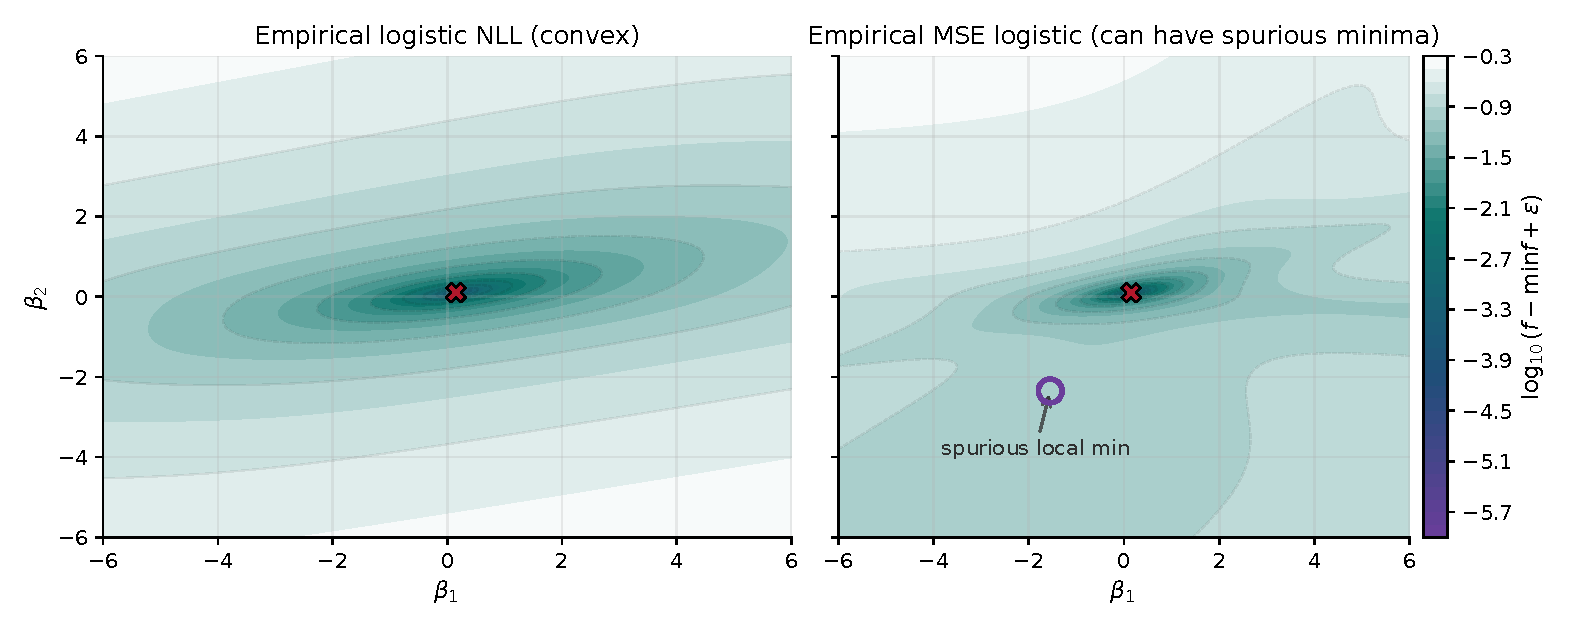
\includegraphics[width=\textwidth]{figures/handouts/convexity_optimization/fig_logistic_empirical_spurious}
  \caption{Empirical logistic landscapes on the dataset in \Cref{ex:logistic-empirical-spurious}.
  The plots show $\log_{10}(f-\min f+\varepsilon)$ for each objective.
  The red X marks the global minimizer in each panel.
  Left: the NLL is convex (one basin).
  Right: the squared-loss objective can have a spurious local minimum (circled), so a local method can get stuck.}
  \label{fig:logistic-empirical-spurious}
\end{figure}

\begin{figure}[t]
  \centering
  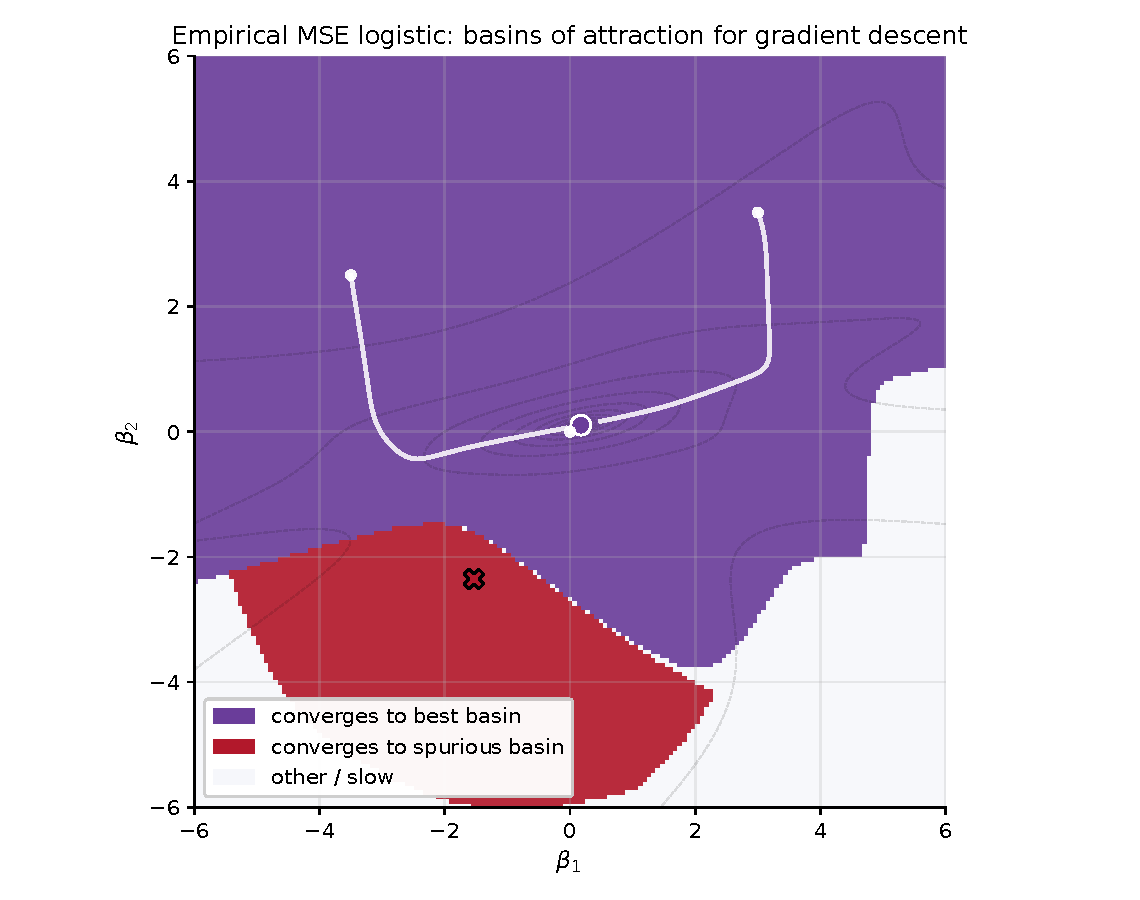
\includegraphics[width=0.92\textwidth]{figures/handouts/convexity_optimization/fig_logistic_empirical_basins}
  \caption{Basins of attraction for gradient descent on the empirical MSE-logistic objective in \Cref{ex:logistic-empirical-spurious}.
  The purple dot and red X mark the two local minimizers.
  Each initialization is colored by which local minimizer fixed-step GD (with $\eta=0.6$) converges to, and the overlaid paths show a few representative trajectories.}
  \label{fig:logistic-empirical-basins}
\end{figure}

Now assume a realizable population model:
\[
Y\mid X=x \sim \mathrm{Bernoulli}(p^\star(x)),
\qquad
p^\star(x) = \sigma(x^\top\beta^\star).
\]
Then the expected squared loss decomposes as
\[
\E\big[(Y-\sigma(X^\top\beta))^2\mid X\big]
= p^\star(X)(1-p^\star(X)) + \big(p^\star(X)-\sigma(X^\top\beta)\big)^2,
\]
so (up to an additive constant) the population objective becomes
\begin{equation}
R(\beta) = \E\big[(\sigma(X^\top\beta)-\sigma(X^\top\beta^\star))^2\big].
\label{eq:logistic-pop-risk}
\end{equation}

\begin{proposition}[One-point monotonicity in the realizable population squared-loss risk]
\label{prop:logistic-pop-one-point}
Assume $\E[\norm{X}_2]<\infty$, and let $R$ be as in \eqref{eq:logistic-pop-risk}. Then for all $\beta$,
\begin{equation}
\ip{\nabla R(\beta)}{\beta-\beta^\star} \ge 0.
\label{eq:one-point}
\end{equation}
In particular, along any ray $\beta(t)=\beta^\star+t(\beta-\beta^\star)$, the function $t\mapsto R(\beta(t))$ is nondecreasing for $t\ge 0$.
\end{proposition}

The next exercise isolates the population monotonicity calculation; structurally it plays the same role as the first-order convexity arguments in the Optimization unit.
\begin{exercise}[One-point monotonicity for realizable MSE-logistic]
\label{ex:logistic-one-point}
Prove \Cref{prop:logistic-pop-one-point}.
Let $\eta=X^\top\beta$ and $\eta^\star=X^\top\beta^\star$.
\begin{enumerate}[leftmargin=*]
  \item Differentiate under the expectation in \eqref{eq:logistic-pop-risk} to show that
  \[
  \nabla R(\beta)
  =2\,\E\Big[(\sigma(\eta)-\sigma(\eta^\star))\,\sigma'(\eta)\,X\Big].
  \]
  \item Show that
  \[
  \ip{\nabla R(\beta)}{\beta-\beta^\star}
  =2\,\E\Big[\sigma'(\eta)\,(\sigma(\eta)-\sigma(\eta^\star))(\eta-\eta^\star)\Big],
  \]
  and conclude it is nonnegative using only that $\sigma$ is increasing and $\sigma'\ge 0$.
  \item Deduce the ray-monotonicity statement by differentiating $g(t)=R(\beta^\star+t(\beta-\beta^\star))$.
\end{enumerate}
\end{exercise}

\SolutionBox[14]{%
\emph{Part (1).}
Differentiate \eqref{eq:logistic-pop-risk} under the expectation:
\[
R(\beta)=\E\big[(\sigma(X^\top\beta)-\sigma(X^\top\beta^\star))^2\big].
\]
Using the chain rule, $\nabla_\beta\sigma(X^\top\beta)=\sigma'(X^\top\beta)\,X$, hence
\[
\nabla R(\beta)
=2\,\E\Big[(\sigma(\eta)-\sigma(\eta^\star))\,\sigma'(\eta)\,X\Big],
\qquad
\eta=X^\top\beta,\ \eta^\star=X^\top\beta^\star.
\]

\emph{Part (2).}
Take the inner product with $(\beta-\beta^\star)$ and use $\ip{X}{\beta-\beta^\star}=\eta-\eta^\star$:
\[
\ip{\nabla R(\beta)}{\beta-\beta^\star}
=2\,\E\Big[\sigma'(\eta)\,(\sigma(\eta)-\sigma(\eta^\star))(\eta-\eta^\star)\Big].
\]
Since $\sigma'(\eta)\ge 0$ and $\sigma$ is increasing, we have
$(\sigma(\eta)-\sigma(\eta^\star))(\eta-\eta^\star)\ge 0$ pointwise.
Therefore the integrand is pointwise nonnegative, and the expectation is nonnegative as claimed.

\emph{Part (3) (ray monotonicity).}
For the ray $\beta(t)=\beta^\star+t(\beta-\beta^\star)$, define $g(t)=R(\beta(t))$.
By the chain rule,
\[
g'(t)=\ip{\nabla R(\beta(t))}{\beta-\beta^\star}\ge 0,
\]
so $t\mapsto R(\beta(t))$ is nondecreasing for $t\ge 0$.
(The argument uses only that the link is increasing with nonnegative derivative, so it holds for any such link function.)%
}

\begin{corollary}[Realizable population MSE-logistic has no spurious local minima]
\label{cor:logistic-pop-no-spurious}
Under the assumptions of \Cref{prop:logistic-pop-one-point}, every local minimizer of the realizable population risk $R$ in \eqref{eq:logistic-pop-risk} is global.
If in addition $\E[XX^\top]\succ 0$, then the unique global minimizer is $\beta^\star$.
\end{corollary}

\begin{exercise}[Stationarity + one-point monotonicity $\Rightarrow$ no spurious local minima]
\label{ex:logistic-one-point-no-spurious}
Prove \Cref{cor:logistic-pop-no-spurious} from \Cref{prop:logistic-pop-one-point}.
\begin{enumerate}[leftmargin=*]
  \item Let $\bar\beta$ be a local minimizer. Since $R$ is differentiable, $\nabla R(\bar\beta)=0$.
  Combine this with \Cref{eq:one-point} to show that
  \[
    0
    = \ip{\nabla R(\bar\beta)}{\bar\beta-\beta^\star}
    = 2\,\E\Big[\sigma'(\bar\eta)\,(\sigma(\bar\eta)-\sigma(\eta^\star))(\bar\eta-\eta^\star)\Big],
  \]
  where $\bar\eta=X^\top\bar\beta$ and $\eta^\star=X^\top\beta^\star$.
  Conclude that $\sigma(X^\top\bar\beta)=\sigma(X^\top\beta^\star)$ almost surely.
  \item Deduce that $R(\bar\beta)=0$, so $\bar\beta$ is a global minimizer.
  \item For uniqueness: show that if $R(\beta)=0$, then $X^\top(\beta-\beta^\star)=0$ almost surely, and deduce $\beta=\beta^\star$ under $\E[XX^\top]\succ 0$.
\end{enumerate}
\end{exercise}

\SolutionBox[14]{%
\emph{Part (1).}
Let $\bar\beta$ be a local minimizer of the differentiable function $R$.
Then $\nabla R(\bar\beta)=0$.
Applying \Cref{prop:logistic-pop-one-point} at $\beta=\bar\beta$ gives
\[
0
= \ip{\nabla R(\bar\beta)}{\bar\beta-\beta^\star}
= 2\,\E\Big[\sigma'(\bar\eta)\,(\sigma(\bar\eta)-\sigma(\eta^\star))(\bar\eta-\eta^\star)\Big],
\qquad \bar\eta=X^\top\bar\beta,\ \eta^\star=X^\top\beta^\star.
\]
The integrand is pointwise nonnegative because $\sigma'(\bar\eta)\ge 0$ and $\sigma$ is increasing, so the expectation can vanish only if the integrand is zero almost surely.
Since $\sigma'(z)>0$ for every finite $z$, this implies
\[
(\sigma(\bar\eta)-\sigma(\eta^\star))(\bar\eta-\eta^\star)=0
\qquad\text{almost surely.}
\]
Because $\sigma$ is strictly increasing, the product above is zero if and only if $\bar\eta=\eta^\star$, equivalently $\sigma(X^\top\bar\beta)=\sigma(X^\top\beta^\star)$ almost surely.

\emph{Part (2).}
If $\sigma(X^\top\bar\beta)=\sigma(X^\top\beta^\star)$ almost surely, then the integrand in \eqref{eq:logistic-pop-risk} vanishes almost surely, so
\[
R(\bar\beta)=\E\big[(\sigma(X^\top\bar\beta)-\sigma(X^\top\beta^\star))^2\big]=0.
\]
Since $R(\beta^\star)=0$ as well, $\bar\beta$ is a global minimizer.

\emph{Part (3) (uniqueness).}
If $R(\beta)=0$, then
\[
\E\big[(\sigma(X^\top\beta)-\sigma(X^\top\beta^\star))^2\big]=0,
\]
so $\sigma(X^\top\beta)=\sigma(X^\top\beta^\star)$ almost surely.
Since $\sigma$ is strictly increasing, this implies $X^\top(\beta-\beta^\star)=0$ almost surely.
Taking expectations yields
$(\beta-\beta^\star)^\top\E[XX^\top](\beta-\beta^\star)=0$.
If $\E[XX^\top]\succ 0$, then the quadratic form is strictly positive unless $\beta=\beta^\star$, so $\beta^\star$ is the unique global minimizer.%
}

The population MSE-logistic risk is nonconvex, but it still has the simple geometry that moving away from $\beta^\star$ does not help along any ray from $\beta^\star$.
This is qualitatively different from objectives like ecological logistic regression (\Cref{sec:ecological-logistic}), where aggregation introduces intrinsic nonconvexity and the landscape can have many distinct basins even under a clean population model.

Even with this benign global geometry, gradient descent can be slow because of saturation and flat plateaus.
The one-point monotonicity in \Cref{prop:logistic-pop-one-point} is a global geometry guarantee, but it is not a rate guarantee.
Far from $\beta^\star$, the squared-loss logistic objective can become very flat because the logistic link saturates:
$\sigma(z)\to 0$ or $1$ and $\sigma'(z)\to 0$ as $|z|\to\infty$.
The squared-loss gradient carries a factor of $\sigma'(X^\top\beta)$, so when the model is very confident (large $|X^\top\beta|$), the gradient can be tiny even if the objective value is not close to its minimum.
This mirrors the ``confidence weights'' story for convex NLL objectives:
in logistic NLL, curvature is largest near the decision boundary, while very confident points contribute little.
For squared loss, that same saturation suppresses the \emph{descent signal} itself, producing plateaus where $\norm{\nabla R(\beta)}_2$ is small even though $R(\beta)-R(\beta^\star)$ is not.

\begin{proposition}[Realizable squared-loss logistic: arbitrarily flat far from $\beta^\star$]
\label{prop:logistic-pop-flat}
Assume $\E[\norm{X}_2]<\infty$ and let $R$ be the realizable population risk \eqref{eq:logistic-pop-risk}.
Define $g(t)=R(t\beta^\star)$ for $t\ge 1$.
Then:
\begin{enumerate}[leftmargin=*]
  \item $g$ is nondecreasing on $[1,\infty)$ and converges to a finite limit $g(\infty)$.
  \item $\lim_{t\to\infty} g'(t)=0$ and $\lim_{t\to\infty}\norm{\nabla R(t\beta^\star)}_2=0$.
  \item If $\Pr(X^\top\beta^\star\neq 0)>0$, then $g(\infty)>0$.
\end{enumerate}
In particular, there are directions along which the landscape becomes arbitrarily flat even though the excess risk stays bounded away from $0$.
\end{proposition}

\emph{Proof idea.} See Exercise~\ref{ex:logistic-plateau}.

\begin{exercise}[Prove the plateau]
\label{ex:logistic-plateau}
In the realizable population model, let $g(t)=R(t\beta^\star)$ for $t\ge 1$.
\begin{enumerate}[leftmargin=*]
  \item Show that
  \[
    g'(t)=2\,\E\big[(\sigma(t\eta^\star)-\sigma(\eta^\star))\,\sigma'(t\eta^\star)\,\eta^\star\big],
    \qquad \eta^\star=X^\top\beta^\star,
  \]
  and conclude that $g$ is nondecreasing (hence $g(t)\to g(\infty)$ since $0\le g(t)\le 1$).
  \item Show that $g'(t)\to 0$ and $\nabla R(t\beta^\star)\to 0$ as $t\to\infty$.
  Interpret this as: \emph{without} a PL/strong-convexity-type condition, small gradient does not imply near-optimality.
  \item Assume $\Pr(\eta^\star\neq 0)>0$.
  Show that $g(\infty)>0$.
\end{enumerate}
\end{exercise}

\SolutionBox[12]{%
Write $\eta^\star=X^\top\beta^\star$ so that $g(t)=\E[(\sigma(t\eta^\star)-\sigma(\eta^\star))^2]$.

\emph{Part (1).}
Differentiate under the expectation:
by the chain rule,
\[
\frac{d}{dt}\sigma(t\eta^\star)=\sigma'(t\eta^\star)\,\eta^\star,
\]
so
\[
g'(t)
=\E\Big[2(\sigma(t\eta^\star)-\sigma(\eta^\star))\cdot \sigma'(t\eta^\star)\,\eta^\star\Big]
=2\,\E\big[(\sigma(t\eta^\star)-\sigma(\eta^\star))\,\sigma'(t\eta^\star)\,\eta^\star\big].
\]
For $t\ge 1$, $\sigma(t\eta^\star)-\sigma(\eta^\star)$ has the same sign as $(t-1)\eta^\star$ since $\sigma$ is increasing.
Because $\sigma'\ge 0$, the integrand is pointwise nonnegative, hence $g'(t)\ge 0$ and $g$ is nondecreasing.
Since $g(t)\in[0,1]$, it follows that $g(t)\to g(\infty)$ for some finite limit $g(\infty)$.

\emph{Part (2).}
For each fixed $\eta^\star\neq 0$, we have $t\eta^\star\to \pm\infty$ and therefore $\sigma'(t\eta^\star)\to 0$ as $t\to\infty$.
Also,
\[
\big|(\sigma(t\eta^\star)-\sigma(\eta^\star))\,\sigma'(t\eta^\star)\,\eta^\star\big|
\le \sigma'(0)\,|\eta^\star|
\le \sigma'(0)\,\norm{\beta^\star}_2\,\norm{X}_2,
\]
which is integrable since $\E[\norm{X}_2]<\infty$.
We will use the following standard fact: if random variables $Z_t$ satisfy $|Z_t|\le W$ with $\E[W]<\infty$ and $Z_t\to 0$ almost surely, then $\E[Z_t]\to 0$.
Applying this fact here gives $g'(t)\to 0$ as $t\to\infty$.

\smallskip
Similarly, differentiating \eqref{eq:logistic-pop-risk} gives
\[
\nabla R(t\beta^\star)
=2\,\E\big[(\sigma(t\eta^\star)-\sigma(\eta^\star))\,\sigma'(t\eta^\star)\,X\big].
\]
The integrand norm is bounded by $2\sigma'(0)\norm{X}_2$, and for each fixed $X$ the factor $\sigma'(t\eta^\star)$ tends to $0$ (or the bracketed term vanishes when $\eta^\star=0$), so the same reasoning lets us pass the limit through the expectation and conclude $\nabla R(t\beta^\star)\to 0$.

\emph{Part (3).}
As $t\to\infty$ we have $\sigma(t\eta^\star)\to 1$ when $\eta^\star>0$, $\sigma(t\eta^\star)\to 0$ when $\eta^\star<0$, and $\sigma(t\eta^\star)=\sigma(\eta^\star)=1/2$ when $\eta^\star=0$.
Since $0\le (\sigma(t\eta^\star)-\sigma(\eta^\star))^2\le 1$, we can apply the same fact (with $W=1$) to pass the limit through the expectation and obtain
\[
g(\infty)=\E\Big[(1-\sigma(\eta^\star))^2\mathbf{1}\{\eta^\star>0\} + \sigma(\eta^\star)^2\mathbf{1}\{\eta^\star<0\}\Big].
\]
If $\Pr(\eta^\star\neq 0)>0$, then the integrand is strictly positive on $\{\eta^\star\neq 0\}$, so $g(\infty)>0$.

Along this ray, the risk can remain bounded away from $0$ while the gradient (and directional derivative) goes to $0$.
Without a condition like PL/strong convexity, a small gradient does not by itself certify near-optimality.
}

Conditions like strong convexity or the PL inequality (\Cref{def:pl-inequality}) prevent this phenomenon: they rule out large flat regions away from the optimum by relating gradient size to suboptimality.
\Cref{prop:logistic-pop-flat} shows the realizable squared-loss logistic risk does not have such a global guarantee in general.

In the realizable population model, the one-point monotonicity in \Cref{prop:logistic-pop-one-point} is a \emph{global} geometric statement.
To get an actual rate for gradient descent, we also need a \emph{local curvature} condition near $\beta^\star$.
One simple sufficient condition is bounded features, which implies local strong convexity (hence a linear rate) around the optimum.

\begin{proposition}[Local linear convergence of gradient descent near $\beta^\star$]
\label{prop:logistic-pop-local-rate}
Assume $\E[XX^\top]\succeq \lambda I_d$ and $\norm{X}_2\le R$ almost surely for some $\lambda,R>0$.
Then at $\beta^\star$,
\[
\Hess R(\beta^\star)\succeq m_0 I_d,
\qquad
m_0 = 2\,\sigma'(R\norm{\beta^\star}_2)^2\,\lambda,
\]
and there exist $r>0$ and constants $0<m\le L<\infty$ such that the population risk $R$ in \eqref{eq:logistic-pop-risk} is $m$-strongly convex and $L$-smooth on the ball $\{\beta:\ \norm{\beta-\beta^\star}_2\le r\}$.
Consequently, gradient descent with step size $1/L$ initialized in this ball satisfies
\[
R(\beta^{(k)})-R(\beta^\star)
\le \left(1-\frac{m}{L}\right)^k\bigl(R(\beta^{(0)})-R(\beta^\star)\bigr)
\qquad\text{(see \citealp[\S9.3]{boyd_vandenberghe_2004_convex}).}
\]
\end{proposition}

\begin{proof}
Differentiate \eqref{eq:logistic-pop-risk} twice.
At $\beta=\beta^\star$, the cross term vanishes and the Hessian simplifies to
\[
\Hess R(\beta^\star)=2\,\E\big[\sigma'(X^\top\beta^\star)^2\,XX^\top\big].
\]
Since $\norm{X^\top\beta^\star}\le \norm{X}_2\norm{\beta^\star}_2\le R\norm{\beta^\star}_2$ almost surely, we have
$\sigma'(X^\top\beta^\star)\ge \sigma'(R\norm{\beta^\star}_2)>0$ almost surely (since $\sigma'$ is even and decreases with $|z|$), hence
\[
\Hess R(\beta^\star)\succeq 2\,\sigma'(R\norm{\beta^\star}_2)^2\,\E[XX^\top]\succeq 2\,\sigma'(R\norm{\beta^\star}_2)^2\,\lambda I_d.
\]
This is the claimed bound with $m_0=2\,\sigma'(R\norm{\beta^\star}_2)^2\,\lambda$.
Because $R$ is twice continuously differentiable and $\norm{X}_2\le R$ almost surely, $\Hess R(\beta)$ varies continuously in $\beta$ and is bounded on compact sets.
Therefore, on a sufficiently small ball around $\beta^\star$, the Hessian is bounded below by (say) $\tfrac12 m_0 I_d$ and above by $L I_d$ for some finite $L$, which gives local strong convexity and smoothness.
The linear convergence rate for gradient descent on an $m$-strongly convex and $L$-smooth function is standard (cited above).
\end{proof}

Under misspecification, hard multimodality can return.
If $p^\star(x)$ is not representable as $\sigma(x^\top\beta)$ (e.g.\ marginalizing over latent classes can yield mixtures of logits), then \eqref{eq:one-point} need not hold, and the population squared-loss risk can become bimodal with spurious local minima.
Benign global geometry often hinges on model and data assumptions.
This is one reason MLE (convex NLL) is often more stable than squared-loss fitting in logistic-type binary regression models.

\begin{example}[Misspecification can create a spurious local minimum for squared-loss logistic regression]
\label{ex:logistic-misspecified-spurious}
Consider a 1D feature $X$ that takes values $\{-2,-1,1,2\}$ with equal probability, and parameterize $\beta=(\beta_0,\beta_1)$ so that $q_\beta(x)=\sigma(\beta_0+\beta_1 x)$.
Let the true conditional probabilities be
\[
p^\star(-2)=0.49,\quad p^\star(-1)=0.87,\quad p^\star(1)=0.92,\quad p^\star(2)=0.36.
\]
This $p^\star$ is not representable as $q_\beta$, since it is not monotone in $x$.

For the population squared-loss risk $R_{\mathrm{MSE}}(\beta)=\E[(q_\beta(X)-p^\star(X))^2]$, a direct evaluation shows two distinct basins:
numerically, evaluating $R_{\mathrm{MSE}}$ on a grid reveals a global minimizer and a spurious local minimizer.
See \Cref{fig:logistic-landscape-2d}.
\end{example}

\begin{figure}[t]
  \centering
  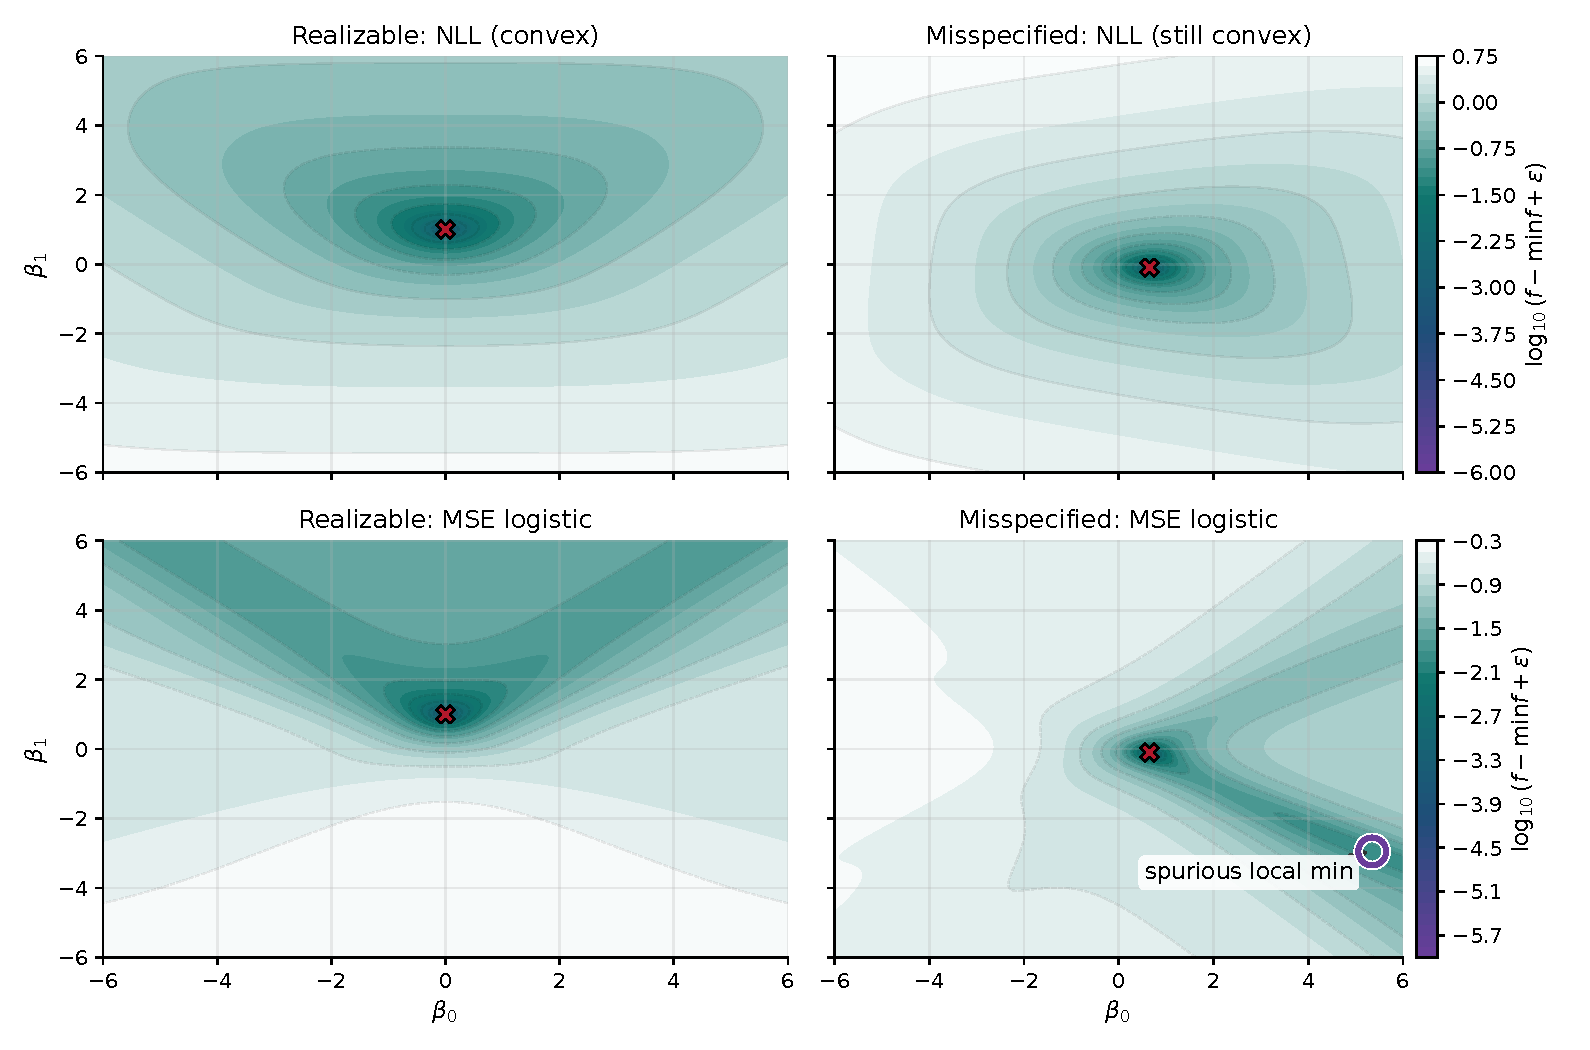
\includegraphics[width=\textwidth]{figures/handouts/convexity_optimization/fig_logistic_landscape_2d}
  \caption{A consistent contourf view of logistic landscapes in a 2D parameterization $\beta=(\beta_0,\beta_1)$.
  The plots show $\log_{10}(f-\min f+\varepsilon)$ for each objective, which makes basins comparable across panels.
  The red X marker indicates the global minimizer in each panel; in the bottom-right plot, the circled point is a spurious local minimum.
  In this example, the NLL landscape is unimodal in both realizable and misspecified settings, while the squared-loss landscape can develop extra basins under misspecification.}
  \label{fig:logistic-landscape-2d}
\end{figure}

% ------------------------------------------------------------
Example~I separates three distinct regimes.
Empirical MSE-logistic can create spurious basins; the realizable population risk has no spurious local minima but can still be slow because of broad plateaus; and misspecification can bring back genuinely wrong stable basins.
The response depends on the regime: use a stable objective when possible, use damping or line search when curvature is unreliable, and use restarts or stronger initializations when multiple basins are present.

% ------------------------------------------------------------
\section[Example II (phase retrieval)]{Example II: multimodality from symmetry, but only global optima in phase retrieval}
\label{sec:phase-retrieval}

In coherent diffraction imaging, optics, and astronomy, sensors measure intensities and lose phase.
A canonical real model is \emph{phase retrieval}:
\[
y_i = (a_i^\top x^\star)^2,\qquad i=1,\dots,m,
\]
where $x^\star\in\R^d$ is the unknown signal and $a_i$ are known sensing vectors.
A standard nonconvex least-squares objective is
\begin{equation}
F(x)=\frac{1}{4m}\sum_{i=1}^m\big((a_i^\top x)^2 - y_i\big)^2.
\label{eq:phase-empirical}
\end{equation}
This objective is nonconvex for structural reasons (it involves squares of linear forms),
and it is \emph{inherently} multimodal because $x^\star$ and $-x^\star$ generate the same data.

Like squared-loss logistic regression, phase retrieval is a smooth, nonconvex least-squares objective.
But here the nonconvexity is driven primarily by a \emph{symmetry}: $x^\star$ and $-x^\star$ generate the same data.
In population (for Gaussian designs), this symmetry produces multiple global optima but \emph{no} suboptimal local minima; the remaining stationary points are saddles.
This is ``benign'' nonconvexity (a strict-saddle picture), and it contrasts with ecological logistic regression (\Cref{sec:ecological-logistic}), where aggregation creates intrinsic nonconvexity and can lead to many distinct basins.
This ``benign geometry'' picture (multiple equivalent global minimizers; strict saddles elsewhere) appears broadly in modern tractable nonconvex problems; see \citet[\S2]{sun_qu_wright_2015_nonconvex_not_scary} and \citet[\S1]{zhang_qu_wright_2020_symmetry_geometry}.

\begin{figure}[t]
  \centering
  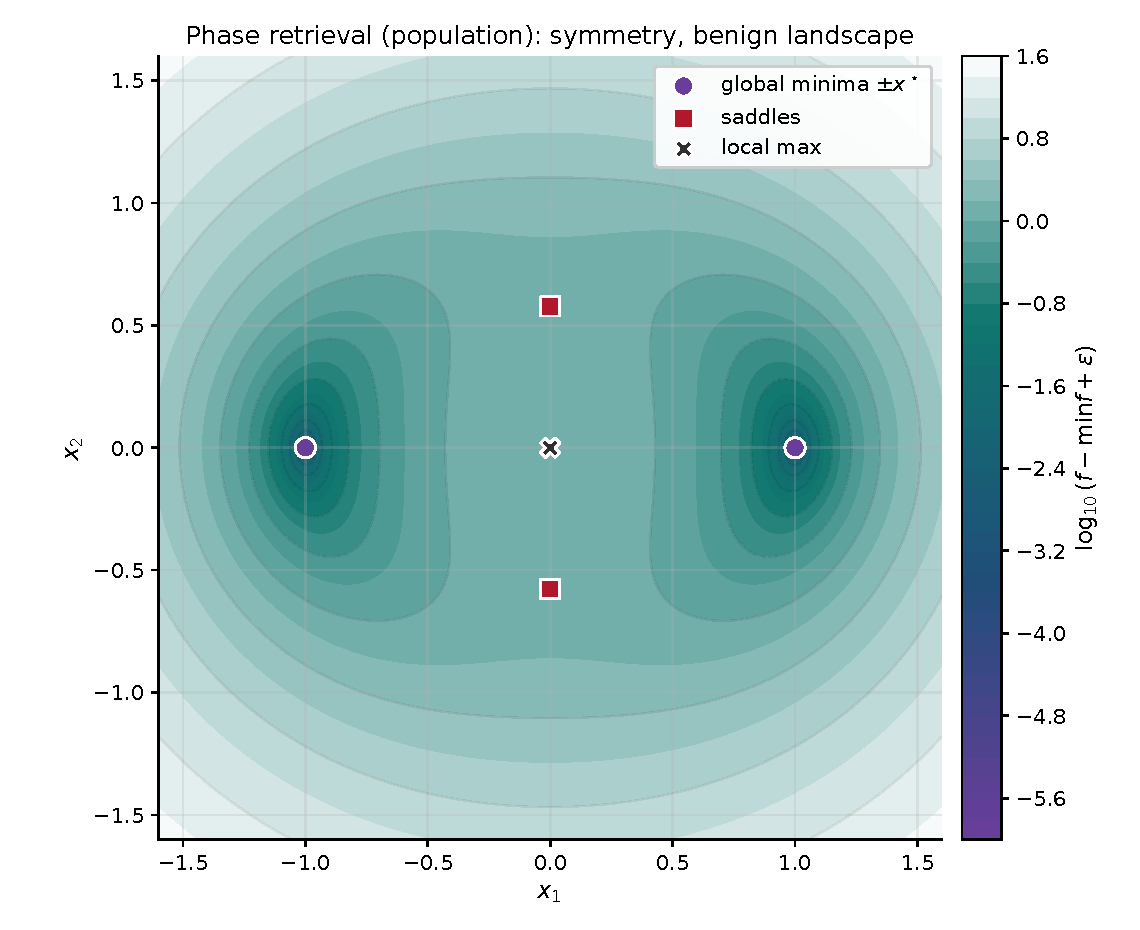
\includegraphics[width=0.86\textwidth]{figures/handouts/convexity_optimization/fig_phase_retrieval_landscape}
  \caption{Population phase retrieval in $d=2$: the landscape is nonconvex and symmetric ($x\sim -x$), but the only local minima are the two global minima $\pm x^\star$; other critical points are saddles or a local maximum at the origin.}
  \label{fig:phase-retrieval-landscape}
\end{figure}

For a clean population model, assume $a\sim N(0,I_d)$ and consider the \emph{population} objective
\begin{equation}
  f(x)=\frac12\,\E\Big[\big((a^\top x)^2 - (a^\top x^\star)^2\big)^2\Big].
  \label{eq:phase-pop}
\end{equation}

\begin{proposition}[Population phase retrieval: nonconvex but no spurious local minima]
\label{prop:phase-retrieval-benign}
For $f$ in \eqref{eq:phase-pop},
\begin{equation}
  f(x)
  =\frac{3}{2}\norm{x}^4 - \norm{x}^2\norm{x^\star}^2 - 2\ip{x}{x^\star}^2 + \frac{3}{2}\norm{x^\star}^4,
  \label{eq:phase-pop-closed-form}
\end{equation}
and the stationary points are:
\begin{enumerate}[leftmargin=*]
  \item global minima $x=\pm x^\star$ (value $0$),
  \item a local maximum at $x=0$,
  \item a saddle set $\{x:\ x\perp x^\star,\ \norm{x}=\norm{x^\star}/\sqrt{3}\}$.
\end{enumerate}
In particular, every local minimum is global.
\end{proposition}

\begin{exercise}[Phase retrieval: derive and classify the population stationary points]
\label{ex:phase-pop-derivation}
Prove \Cref{prop:phase-retrieval-benign}.
\begin{enumerate}[leftmargin=*]
  \item Expand \eqref{eq:phase-pop} and use the Gaussian fourth-moment identities
  \[
  \E[(a^\top u)^4]=3\norm{u}^4,
  \qquad
  \E[(a^\top u)^2(a^\top v)^2]=\norm{u}^2\norm{v}^2 + 2\ip{u}{v}^2,
  \]
  to obtain \eqref{eq:phase-pop-closed-form}.
  \item Differentiate \eqref{eq:phase-pop-closed-form} to get an explicit formula for $\nabla f(x)$.
  \item Solve $\nabla f(x)=0$ by decomposing $x=\alpha x^\star + u$ with $u\perp x^\star$.
  \item Classify the stationary points as global minima, a local maximum, and a saddle set.
\end{enumerate}
\end{exercise}

\SolutionBox[22]{%
\emph{Part (1) (closed form).}
Expanding the square in \eqref{eq:phase-pop} gives
\[
f(x)
=\frac12\,\E\big[(a^\top x)^4\big]
\;-\;\E\big[(a^\top x)^2(a^\top x^\star)^2\big]
\;+\;\frac12\,\E\big[(a^\top x^\star)^4\big].
\]
Apply the stated Gaussian fourth-moment identities with $u=x$ and $v=x^\star$ to get
\[
\E[(a^\top x)^4]=3\norm{x}^4,\qquad
\E[(a^\top x^\star)^4]=3\norm{x^\star}^4,
\]
and
\[
\E[(a^\top x)^2(a^\top x^\star)^2]=\norm{x}^2\norm{x^\star}^2 + 2\ip{x}{x^\star}^2.
\]
Substituting yields \eqref{eq:phase-pop-closed-form}.

\emph{Part (2) (gradient).}
Differentiate \eqref{eq:phase-pop-closed-form}:
\[
\nabla f(x)
= 6\norm{x}^2 x - 2\norm{x^\star}^2 x - 4\ip{x}{x^\star}x^\star
= (6\norm{x}^2-2\norm{x^\star}^2)x - 4\ip{x}{x^\star}x^\star.
\]

\emph{Part (3) (stationary points).}
Let $r=\norm{x^\star}_2$ and decompose $x=\alpha x^\star + u$ with $u\perp x^\star$.
Then $\ip{x}{x^\star}=\alpha r^2$ and $\norm{x}^2=\alpha^2r^2+\norm{u}^2$.
Setting $\nabla f(x)=0$ and matching the $u$ and $x^\star$ components gives
\[
(6\norm{x}^2-2r^2)\,u=0,
\qquad
\alpha\,(6\norm{x}^2-6r^2)=0.
\]
If $u=0$, then either $\alpha=0$ (so $x=0$) or $\norm{x}^2=r^2$ (so $\alpha=\pm 1$ and $x=\pm x^\star$).
If $u\neq 0$, then the first equation forces $\norm{x}^2=r^2/3$, and the second forces $\alpha=0$, hence
$x\perp x^\star$ and $\norm{x}=r/\sqrt{3}$.
This gives exactly the stationary-point list in \Cref{prop:phase-retrieval-benign}.

\emph{Part (4) (classification).}
Since $f$ in \eqref{eq:phase-pop} is an expectation of a square, $f(x)\ge 0$ for all $x$.
Also $f(\pm x^\star)=0$, so $\pm x^\star$ are global minima.

For $x=0$, the expansion \eqref{eq:phase-pop-closed-form} shows
\[
f(0)-f(x)= r^2\norm{x}^2 + 2\ip{x}{x^\star}^2 - \frac{3}{2}\norm{x}^4,
\]
which is strictly positive for all sufficiently small $x\neq 0$ (the quadratic term dominates), so $x=0$ is a local maximum.

Finally, if $x\perp x^\star$ and $\norm{x}=r/\sqrt{3}$, then the univariate restriction $t\mapsto f(x+t x^\star)$ has negative second derivative at $t=0$, so there is a direction of negative curvature.
Hence these points are saddles, and every local minimum is global.%
}

This is symmetry-driven nonconvexity with a strict-saddle geometry:
every non-optimal stationary point has a direction of negative curvature.

Phase retrieval is typically approached via the two-stage template in \Cref{alg:two-stage-template}:
use a cheap global initializer, then run a local method.
In the Gaussian model, there is a clean way to build a provably good direction estimate from a simple moment identity.
Assume the noiseless Gaussian design model $a_i \stackrel{\mathrm{iid}}{\sim} N(0,I_d)$ with measurements $y_i=(a_i^\top x^\star)^2$.
Define the \emph{spectral matrix}
\[
  Y = \frac{1}{m}\sum_{i=1}^m y_i a_i a_i^\top.
\]
Also define the radius estimate
\[
  \hat r^2 = \frac{1}{m}\sum_{i=1}^m y_i,
\]
which satisfies $\E[\hat r^2]=\norm{x^\star}_2^2$.
If $\hat u$ is a unit-norm top eigenvector of $Y$, then the standard spectral initializer is $x^{(0)}=\hat r\,\hat u$.

The next proposition explains why this initialization is reasonable.
It shows that (i) the population matrix $\E[Y]$ has a unique leading eigenvector in the $x^\star$ direction, and (ii) if the empirical $Y$ is close to $\E[Y]$ in operator norm then its leading eigenvector must be close to $\pm x^\star/\norm{x^\star}_2$.
(Here $\norm{M}_{\mathrm{op}}$ denotes the operator norm, i.e.\ the largest absolute eigenvalue for a symmetric matrix $M$.)

\begin{proposition}[Gaussian phase retrieval: why the spectral initializer points at $x^\star$]
\label{prop:phase-spectral-init}
Assume $x^\star\neq 0$, let $a\sim N(0,I_d)$, and set $y=(a^\top x^\star)^2$.
Write $r=\norm{x^\star}_2$ and $u^\star=x^\star/r$.
Define the population matrix
\[
  Y_{\mathrm{pop}} = \E\big[y\,a a^\top\big]
  = \E\big[(a^\top x^\star)^2 a a^\top\big].
\]
Then
\[
  Y_{\mathrm{pop}}=r^2 I_d + 2x^\star(x^\star)^\top,
\]
so the unique leading eigenvector of $Y_{\mathrm{pop}}$ is $u^\star$.
Moreover, if $Y$ is any symmetric matrix satisfying
\[
\norm{Y-Y_{\mathrm{pop}}}_{\mathrm{op}} \le \varepsilon\, r^2
\qquad\text{for some }\varepsilon\in(0,1),
\]
then for every unit-norm leading eigenvector $\hat u$ of $Y$ there exists a sign $s\in\{\pm 1\}$ such that
$\norm{\hat u-su^\star}_2\le \sqrt{2\varepsilon}$.
\end{proposition}

\begin{exercise}[Phase retrieval: why spectral initialization points at $x^\star$]
\label{ex:phase-spectral-spike}
Prove \Cref{prop:phase-spectral-init}.
Conclude that if the empirical matrix $Y$ is close to $Y_{\mathrm{pop}}$ in operator norm, then its top eigenvector is close to $\pm u^\star$ and the spectral initializer $x^{(0)}=\hat r\,\hat u$ is close to $\pm x^\star$.
\emph{Hint:} to compute $Y_{\mathrm{pop}}$, you can either compute entries using the Gaussian fourth-moment identity
$\E[a_i a_j a_k a_\ell]=\delta_{ij}\delta_{k\ell}+\delta_{ik}\delta_{j\ell}+\delta_{i\ell}\delta_{jk}$,
or compute the entries directly by expanding.
For the perturbation bound, compare quadratic forms $v^\top Y v$ and use $|v^\top (Y-Y_{\mathrm{pop}}) v|\le \norm{Y-Y_{\mathrm{pop}}}_{\mathrm{op}}$ for unit $v$.
Finally, explain in a sentence why one expects $\norm{Y-Y_{\mathrm{pop}}}_{\mathrm{op}}$ to be small when $m$ is large in the Gaussian model.
\end{exercise}

\SolutionBox[20]{%
Write $u=x^\star$ and expand $y=(a^\top u)^2=\sum_{k,\ell} u_k u_\ell a_k a_\ell$.
For each entry $(i,j)$,
\[
\E\!\big[y\,a_i a_j\big]
=\sum_{k,\ell} u_k u_\ell\,\E[a_i a_j a_k a_\ell]
=\sum_{k,\ell} u_k u_\ell\bigl(\delta_{ij}\delta_{k\ell}+\delta_{ik}\delta_{j\ell}+\delta_{i\ell}\delta_{jk}\bigr).
\]
The first term gives $\delta_{ij}\sum_k u_k^2=\delta_{ij}\norm{u}_2^2$.
The second and third terms each give $u_i u_j$.
Thus $\E[y\,a_i a_j]=\norm{u}_2^2\,\delta_{ij}+2u_i u_j$, i.e.
$Y_{\mathrm{pop}}=\norm{u}_2^2 I_d + 2uu^\top$.

For eigenvalues, note that $Y_{\mathrm{pop}}u=(\norm{u}_2^2+2\norm{u}_2^2)u=3\norm{u}_2^2 u$.
If $w\perp u$, then $uu^\top w=0$ so $Y_{\mathrm{pop}}w=\norm{u}_2^2 w$.
Hence the unique top eigenspace is $\mathrm{span}\{u\}$.

Let $r=\norm{u}_2$ and $u^\star=u/r$.
Let $\hat u$ be a unit top eigenvector of $Y$.
Write $E=Y-Y_{\mathrm{pop}}$ and assume $\norm{E}_{\mathrm{op}}\le \varepsilon r^2$.
Then
\[
\hat u^\top Y_{\mathrm{pop}} \hat u
= \hat u^\top Y \hat u - \hat u^\top E \hat u
\ge \lambda_{\max}(Y) - \norm{E}_{\mathrm{op}}
\ge (u^\star)^\top Y u^\star - \norm{E}_{\mathrm{op}}
\ge 3r^2 - 2\varepsilon r^2.
\]
On the other hand,
$
\hat u^\top Y_{\mathrm{pop}} \hat u
= r^2 + 2r^2\,|\ip{\hat u}{u^\star}|^2.
$
Combining gives $|\ip{\hat u}{u^\star}|^2\ge 1-\varepsilon$.
Choosing the sign that maximizes the inner product,
\[
\min\{\norm{\hat u-u^\star}_2,\norm{\hat u+u^\star}_2\}^2
=2\bigl(1-|\ip{\hat u}{u^\star}|\bigr)
\le 2\bigl(1-|\ip{\hat u}{u^\star}|^2\bigr)
\le 2\varepsilon.
\]

The matrix $Y$ is an empirical average of i.i.d.\ symmetric matrices with mean $Y_{\mathrm{pop}}$.
To make this quantitative in high dimensions, one uses concentration inequalities for random matrices to bound $\norm{Y-Y_{\mathrm{pop}}}_{\mathrm{op}}$ with high probability; see \citet[\S2.2]{zhang_qu_wright_2020_symmetry_geometry} for discussion and references.
These probability tools are largely orthogonal to our focus here.%
}

Once you have an initialization that is close to $\pm x^\star$, the local stage behaves like the convex story again.
In the Gaussian population objective, $\pm x^\star$ are not only global minima: they are \emph{locally strongly convex} minima, so the standard local strong-convexity analysis from the Optimization unit gives a linear rate while the iterates remain in that neighborhood.

\begin{exercise}[Phase retrieval: local convexity near $\pm x^\star$ in the population objective]
\label{ex:phase-pop-local-strong-convex}
For the population objective $f$ in \eqref{eq:phase-pop-closed-form}, compute the Hessian $\Hess f(x)$ and show that
\[
\Hess f(x^\star)=4\norm{x^\star}_2^2 I_d + 8x^\star(x^\star)^\top.
\]
Deduce the eigenvalues of $\Hess f(x^\star)$ and interpret this as a local condition-number statement near $x^\star$.
\end{exercise}

\SolutionBox[12]{%
Differentiate the gradient formula in the solution to \Cref{ex:phase-pop-derivation}:
for $x\in\R^d$,
\[
\Hess f(x)=12xx^\top + (6\norm{x}_2^2-2\norm{x^\star}_2^2)I_d - 4x^\star(x^\star)^\top.
\]
At $x=x^\star$ this becomes
\[
\Hess f(x^\star)=(12-4)x^\star(x^\star)^\top + 4\norm{x^\star}_2^2 I_d
=8x^\star(x^\star)^\top + 4\norm{x^\star}_2^2 I_d.
\]
Along $u^\star=x^\star/\norm{x^\star}_2$ the eigenvalue is $12\norm{x^\star}_2^2$, and along any direction orthogonal to $x^\star$ the eigenvalue is $4\norm{x^\star}_2^2$.
So near $x^\star$ the population objective is well conditioned (local condition number $3$), which is exactly the regime where local methods behave like in the convex case.%
}

These pieces give the standard Gaussian-model story:
spectral initialization supplies a direction close to $\pm x^\star$, and the local geometry near $\pm x^\star$ is strongly convex, so local methods converge quickly once initialized there.
Rigorous finite-sample analyses follow this template; see \citet[\S2.2]{zhang_qu_wright_2020_symmetry_geometry} and references therein.

Phase retrieval shows a different kind of nonconvexity.
The sign symmetry creates multiple optima, but they are equivalent, and the remaining stationary points are saddles rather than bad local minima.
The right response is therefore not exhaustive global search; it is a coarse initializer, such as a spectral method, followed by local refinement inside the basin of $\pm x^\star$.



% ------------------------------------------------------------
\section[Example III (ecological logistic)]{Example III: hard nonconvexity from aggregation in ecological logistic regression}
\label{sec:ecological-logistic}

In some applications we observe covariates at the unit level but only aggregated outcomes.
For example, we might see covariates $x_{g,1},\dots,x_{g,n_g}$ for individuals in a group (a precinct, a cohort, a batch),
but instead of observing the binary outcomes $Y_{g,i}\in\{0,1\}$ we only observe the group total
\[
Z_g = \sum_{i=1}^{n_g} Y_{g,i}.
\]
Many different binary vectors $(Y_{g,1},\dots,Y_{g,n_g})$ can produce the same total $Z_g$, so the likelihood for $\beta$ must marginalize over a large discrete set of latent ``assignments.''

Assume a logistic model at the unit level:
\[
\Pr(Y_{g,i}=1\mid x_{g,i},\beta)=\sigma(x_{g,i}^\top\beta),
\qquad i=1,\dots,n_g,
\]
with conditional independence across $i$ given the covariates.
Write $p_{g,i}(\beta)=\sigma(x_{g,i}^\top\beta)$.
Then $Z_g$ is a sum of independent but non-identically distributed Bernoulli random variables (a Poisson--binomial model), and the marginal likelihood contains $\binom{n_g}{z_g}$ terms.
The resulting negative log-likelihood is typically nonconvex in $\beta$.
This combinatorial marginalization also creates a separate difficulty that is easy to miss if we focus only on the geometry:
when $n_g$ is large, the likelihood term $\Pr(Z_g=z_g\mid x_{g,1},\dots,x_{g,n_g},\beta)$ can be expensive to evaluate repeatedly inside an optimizer.
The naive computation is literally a sum over $\binom{n_g}{z_g}$ assignments (as in \Cref{ex:eco-logistic-nonconvex}), which is intractable for large groups.
This ``optimization + marginalization'' pattern is common in latent-variable models: hard landscapes and expensive objective evaluations can come together.

An empirical negative log-likelihood objective for $G$ independent groups is
\begin{equation}
  f(\beta)
  =
  -\frac{1}{G}\sum_{g=1}^G \log \Pr(Z_g=z_g \mid x_{g,1},\dots,x_{g,n_g},\beta).
  \label{eq:eco-logistic-obj}
\end{equation}
Two edge cases are instructive.
In the special case where the covariates are constant within each group ($x_{g,i}\equiv x_g$), we have
$Z_g\sim \mathrm{Binomial}(n_g,\sigma(x_g^\top\beta))$, and \eqref{eq:eco-logistic-obj} reduces to the usual convex binomial logistic-regression objective from the Optimization unit.
At the other extreme, if $d=1$ with $\beta=(\beta_0,\beta_1)$ and each group contains covariates in $\pm$ pairs (for every $x$ the value $-x$ appears with the same multiplicity), then the marginal likelihood is symmetric in the slope: it is unchanged under $\beta_1\mapsto -\beta_1$.
This kind of symmetry reflects a genuine non-identifiability from totals alone.

\begin{exercise}[Ecological logistic regression: two easy special cases]
\label{ex:eco-logistic-edge-cases}
\begin{enumerate}[leftmargin=*]
  \item Suppose $x_{g,i}\equiv x_g$ within each group.
  Show that $Z_g\sim \mathrm{Binomial}(n_g,\sigma(x_g^\top\beta))$ and conclude that the corresponding negative log-likelihood is convex in $\beta$.
  \item Assume $d=1$ with $\beta=(\beta_0,\beta_1)$ and suppose the multiset $\{x_1,\dots,x_n\}$ is symmetric: for every $x$ it contains $-x$ with the same multiplicity.
  Show that, for every $z$,
  \[
    \Pr(Z=z\mid x_1,\dots,x_n,(\beta_0,\beta_1))
    =
    \Pr(Z=z\mid x_1,\dots,x_n,(\beta_0,-\beta_1)).
  \]
  Conclude that the likelihood for $\beta_1$ is an even function, so the sign of the slope is not identifiable from $Z$ alone in such a balanced design.
\end{enumerate}
\end{exercise}

\SolutionBox[14]{%
\emph{Part (1).}
If $x_{g,i}\equiv x_g$, then conditional on $x_g$ the unit-level outcomes are i.i.d.\ Bernoulli with success probability $\sigma(x_g^\top\beta)$.
Therefore $Z_g=\sum_{i=1}^{n_g}Y_{g,i}\sim \mathrm{Binomial}(n_g,\sigma(x_g^\top\beta))$.
Up to an additive constant (independent of $\beta$), the per-group negative log-likelihood can be written as a function of the scalar $\eta=x_g^\top\beta$:
\[
\ell_g(\beta)
= -z_g\,\eta + n_g\log(1+e^\eta).
\]
Since $\frac{d^2}{d\eta^2}\ell_g(\eta)=n_g\,\sigma'(\eta)\ge 0$, the map $\eta\mapsto \ell_g(\eta)$ is convex.
Composing a convex function with a linear map $\beta\mapsto x_g^\top\beta$ preserves convexity, so $\ell_g$ is convex in $\beta$.
Summing over $g$ preserves convexity, hence the full objective is convex.

\emph{Part (2).}
Write $p_i(\beta_0,\beta_1)=\sigma(\beta_0+\beta_1 x_i)$.
Replacing $\beta_1$ by $-\beta_1$ replaces $p_i$ by $\tilde p_i=\sigma(\beta_0-\beta_1 x_i)$.
By the assumed symmetry of the multiset $\{x_i\}$, the multiset $\{\tilde p_i\}$ is the same as $\{p_i\}$ up to a permutation (each $x$ is paired with $-x$).
But the distribution of $Z=\sum_i Y_i$ depends only on the multiset of success probabilities, not on how they are ordered, so $\Pr(Z=z\mid x_1,\dots,x_n,(\beta_0,\beta_1))=\Pr(Z=z\mid x_1,\dots,x_n,(\beta_0,-\beta_1))$ for every $z$.
Thus the likelihood is an even function of $\beta_1$, which means the sign of the slope is not identifiable from totals in this balanced design.%
}

This example ties directly to the empirical-versus-population theme from Example~I.
There the bad basins can be a finite-sample artifact under benign population geometry; here the nonconvexity is intrinsic, because even under the correct model and infinite data aggregation forces us to marginalize over discrete latent assignments.
That marginalization step is also the bridge to the Expectation--maximization subsection of the Augmented-state optimization unit: once the assignments are latent, the natural algorithmic object is the EM update map, which alternates exact conditional expectations with parameter updates, rather than a single closed-form convex objective.

To emphasize this, it is useful to look at a \emph{population} version of \eqref{eq:eco-logistic-obj}.
Let $X=(x_1,\dots,x_n)$ denote a random group of covariates and let $Z$ be generated from the model under a true parameter $\beta^\star$.
Define the population objective
\[
F(\beta)=\E\big[-\log \Pr(Z\mid X,\beta)\big].
\]
Because the model is correctly specified, $F$ is minimized at (an observationally equivalent version of) $\beta^\star$.
However, as \Cref{fig:eco-logistic-pop-landscape} illustrates, $F$ can still have multiple separated basins and spurious local minima.

\begin{figure}[H]
  \centering
  \input{figures/handouts/convexity_optimization/fig_ecological_logistic_population_landscape}
  \caption{A toy \emph{population} objective for ecological logistic regression in a 2D parameterization $\beta=(\beta_0,\beta_1)$.
  Each group has $n=6$ units and is equally likely to have covariates $(-4,-3,-2,2,3,4)$, $(-3,-1,1,2,3,4)$, or $(-2,-1,1,2,3,4)$ (in $d=1$); outcomes are generated under $\beta^\star=(0.3,1.2)$.
  The plot shows $\log_{10}(F-\min F+\varepsilon)$, as in \Cref{fig:logistic-landscape-2d}; the red X marks $\beta^\star$ and the open circles mark three spurious local minima in this toy example.}
  \label{fig:eco-logistic-pop-landscape}
\end{figure}

\begin{exercise}[Ecological logistic regression: marginalization and nonconvexity]
\label{ex:eco-logistic-nonconvex}
Fix one group with covariates $x_1,\dots,x_n\in\R^d$ and observe $Z=z$.
Let $p_i(\beta)=\sigma(x_i^\top\beta)$.
\begin{enumerate}[leftmargin=*]
  \item Show that
  \[
    \Pr(Z=z\mid x_1,\dots,x_n,\beta)
    =
    \sum_{\substack{S\subseteq\{1,\dots,n\}\\|S|=z}}
    \ \prod_{i\in S} p_i(\beta)\prod_{j\notin S}\bigl(1-p_j(\beta)\bigr).
  \]
  Interpret this as summing over all ways to choose which $z$ units are the successes.
  \item Specialize to $n=2$ and $z=1$ in $d=1$ with covariates $x_1=a$ and $x_2=b$.
  Let $\ell(\beta)$ be the negative log-likelihood $-\log \Pr(Z=1\mid a,b,\beta)$ with no regularization.
  Show that $\ell''(0)=\tfrac12 ab$.
  Conclude that $\ell$ is not convex whenever $ab<0$.
\end{enumerate}
\end{exercise}

\SolutionBox[20]{%
\emph{Part (1).}
Condition on the covariates.
For any binary vector $y=(y_1,\dots,y_n)\in\{0,1\}^n$, conditional independence gives
\[
\Pr(Y_1=y_1,\dots,Y_n=y_n\mid x_1,\dots,x_n,\beta)
=
\prod_{i=1}^n p_i(\beta)^{y_i}\bigl(1-p_i(\beta)\bigr)^{1-y_i}.
\]
The event $\{Z=z\}$ is the union of all assignments $y$ with exactly $z$ ones, so summing over those assignments yields
\[
\Pr(Z=z\mid x_1,\dots,x_n,\beta)
=
\sum_{\substack{y\in\{0,1\}^n\\ \sum_i y_i=z}}
\ \prod_{i=1}^n p_i(\beta)^{y_i}\bigl(1-p_i(\beta)\bigr)^{1-y_i}.
\]
Reindexing the sum by the subset $S=\{i:\ y_i=1\}$ (which has $|S|=z$) gives the stated formula.

\emph{Part (2).}
For $n=2$ and $z=1$, let $p_1(\beta)=\sigma(a\beta)$ and $p_2(\beta)=\sigma(b\beta)$.
Then
\[
q(\beta)=\Pr(Z=1\mid a,b,\beta)
 = p_1(1-p_2) + (1-p_1)p_2
 = p_1+p_2-2p_1p_2,
\]
and $\ell(\beta)=-\log q(\beta)$.
At $\beta=0$ we have $p_1=p_2=\tfrac12$, so $q(0)=\tfrac12$.
Also $p_1'(\beta)=a\,p_1(1-p_1)$ and $p_2'(\beta)=b\,p_2(1-p_2)$, so $p_1'(0)=a/4$ and $p_2'(0)=b/4$.
A direct differentiation gives $q'(0)=0$ and
\[
q''(0)=-4p_1'(0)p_2'(0)=-4\cdot\frac{a}{4}\cdot\frac{b}{4}=-\frac{ab}{4}.
\]
Since $\ell'=-q'/q$ and $q'(0)=0$, we have $\ell''(0)=-(q''(0)/q(0))$ and therefore
\[
\ell''(0)
=-\frac{q''(0)}{q(0)}
=-\frac{-ab/4}{1/2}
=\frac{ab}{2}.
\]
If $ab<0$, then $\ell''(0)<0$, so $\ell$ is not convex.
}

Even though the landscape can be globally hard (and even the population objective can have spurious basins, as in \Cref{fig:eco-logistic-pop-landscape}), there is still a familiar ``convex'' story \emph{locally} around the true parameter under correct specification.
When the model is locally identifiable, the population objective has a neighborhood of $\beta^\star$ on which it is convex (indeed strongly convex).
One convenient way to see this in ecological logistic regression is to expose the probabilistic structure behind the gradient and Hessian: the observed-data objective involves marginalizing over latent assignments, and its Hessian can be written as a difference of two covariance matrices.
After averaging over the random total $Z$ under the true model, that difference becomes a covariance by the law of total covariance.

\begin{exercise}[Ecological logistic regression: DC structure and local convexity near $\beta^\star$]
\label{ex:eco-logistic-pop-local-convex}
Fix covariates $x_1,\dots,x_n\in\R^d$.
For $\beta\in\R^d$, let $V_1,\dots,V_n$ be independent Bernoulli random variables with
\[
\Pr(V_j=1\mid x_j,\beta)=\sigma(x_j^\top\beta),
\qquad j=1,\dots,n,
\]
and define
\[
U = \sum_{j=1}^n x_j V_j,
\qquad
Z = \sum_{j=1}^n V_j.
\]
For an observed total $Z=z$, write $L_z(\beta)=-\log \Pr(Z=z\mid x_1,\dots,x_n,\beta)$.
\begin{enumerate}[leftmargin=*]
  \item Show the \emph{difference-of-convex (DC)} form
  \[
  L_z(\beta)
  =\sum_{j=1}^n \log\bigl(1+e^{x_j^\top\beta}\bigr)
  -\log\left(\sum_{\substack{S\subseteq\{1,\dots,n\}\\|S|=z}} \exp\Big(\sum_{j\in S} x_j^\top\beta\Big)\right).
  \]
  \item Show that $\nabla L_z(\beta)=\E[U]-\E[U\mid Z=z]$.
  \item Show that $\Hess L_z(\beta)=\mathrm{Cov}(U)-\mathrm{Cov}(U\mid Z=z)$.
  (Hint: for $g(\beta)=\log\sum_k e^{a_k^\top\beta}$, the Hessian is the covariance of the vectors $\{a_k\}$ under the corresponding softmax weights.)
  \item Consider the population objective $F(\beta)=\E[L_Z(\beta)]$ when $Z$ is generated under a true parameter $\beta^\star$.
  Assuming the outer expectation defining $F$ can be differentiated twice under the integral sign, use the conditional law of total covariance,
  \[
    \mathrm{Cov}(U\mid X)=\E[\mathrm{Cov}(U\mid Z,X)\mid X] + \mathrm{Cov}(\E[U\mid Z,X]\mid X),
  \]
  to show that
  \[
    \E\big[\Hess L_Z(\beta^\star)\mid X\big]
    = \mathrm{Cov}\big(\E[U\mid Z,X]\mid X\big)\succeq 0.
  \]
  Deduce that
  \[
    \Hess F(\beta^\star)
    = \E\Big[\mathrm{Cov}\big(\E[U\mid Z,X]\mid X\big)\Big]\succeq 0.
  \]
  Conclude that if $\Hess F(\beta^\star)\succ 0$, then $F$ is locally strongly convex on a neighborhood of $\beta^\star$.
\end{enumerate}
\end{exercise}

\SolutionBox[22]{%
\emph{Part (1).}
Write $\eta_j=x_j^\top\beta$ and $p_j=\sigma(\eta_j)=e^{\eta_j}/(1+e^{\eta_j})$.
For any subset $S$ with $|S|=z$,
\[
\Pr(V_j=1\ \forall j\in S,\ V_j=0\ \forall j\notin S\mid x_1,\dots,x_n,\beta)
=\prod_{j\in S}p_j\prod_{j\notin S}(1-p_j)
=\frac{\exp(\sum_{j\in S}\eta_j)}{\prod_{j=1}^n(1+e^{\eta_j})}.
\]
Summing over all $S$ with $|S|=z$ gives
\[
\Pr(Z=z\mid x_1,\dots,x_n,\beta)
=\frac{\sum_{|S|=z}\exp(\sum_{j\in S}\eta_j)}{\prod_{j=1}^n(1+e^{\eta_j})}.
\]
Taking $-\log$ yields the stated DC representation.

\emph{Parts (2) and (3).}
The first term in $L_z$ has gradient $\sum_j \sigma(\eta_j)x_j$ and Hessian $\sum_j \sigma'(\eta_j)x_jx_j^\top$.
Since $U=\sum_j x_j V_j$ with independent Bernoulli coordinates, these are exactly $\E[U]$ and $\mathrm{Cov}(U)$.

For the second term, define a probability distribution on subsets $S$ of size $z$ by
\[
w_S(\beta)\propto \exp\Big(\sum_{j\in S}x_j^\top\beta\Big),
\qquad |S|=z.
\]
This is the conditional law of the success set $\{j:\ V_j=1\}$ given $Z=z$ under parameter $\beta$.
Therefore
\[
\nabla \log\Big(\sum_{|S|=z} e^{\sum_{j\in S}x_j^\top\beta}\Big)
  = \sum_{|S|=z} w_S(\beta)\sum_{j\in S}x_j
  = \E[U\mid Z=z],
\]
and differentiating once more gives
\[
\Hess\!\left(\log\Big(\sum_{|S|=z} e^{\sum_{j\in S}x_j^\top\beta}\Big)\right)
=\mathrm{Cov}(U\mid Z=z),
\]
which yields $\nabla L_z=\E[U]-\E[U\mid Z=z]$ and $\Hess L_z=\mathrm{Cov}(U)-\mathrm{Cov}(U\mid Z=z)$.

\emph{Part (4).}
Now let $X=(x_1,\dots,x_n)$ be random, and assume we may differentiate the outer expectation in $F(\beta)=\E[L_Z(\beta)]$ twice under the integral sign.
Conditional on $X$ and at $\beta^\star$, take expectations over $Z$:
\[
\E\big[\Hess L_Z(\beta^\star)\mid X\big]
=\mathrm{Cov}(U\mid X)-\E[\mathrm{Cov}(U\mid Z,X)\mid X].
\]
By the conditional law of total covariance,
\[
\mathrm{Cov}(U\mid X)
=\E[\mathrm{Cov}(U\mid Z,X)\mid X] + \mathrm{Cov}(\E[U\mid Z,X]\mid X),
\]
so the difference is
\[
\E\big[\Hess L_Z(\beta^\star)\mid X\big]
=\mathrm{Cov}(\E[U\mid Z,X]\mid X)\succeq 0.
\]
Taking outer expectations gives
\[
\Hess F(\beta^\star)
=\E\big[\Hess L_Z(\beta^\star)\big]
=\E\Big[\mathrm{Cov}(\E[U\mid Z,X]\mid X)\Big]\succeq 0.
\]
If this unconditional Hessian is positive definite, then by continuity of $\Hess F$ there exists a radius $r>0$ such that $\Hess F(\beta)\succeq \tfrac12 \Hess F(\beta^\star)\succ 0$ on $\{\beta:\ \norm{\beta-\beta^\star}_2\le r\}$, which implies local strong convexity of $F$ on that neighborhood.%
}

This example still fits the two-stage template in \Cref{alg:two-stage-template}, but the coarse stage is less structured.
In practice, one often uses multiple random starts or a warm start from a crude convex surrogate, then runs a local optimizer with line search or damping on the true nonconvex objective \eqref{eq:eco-logistic-obj} and keeps the best solution found.

Ecological logistic regression is the genuinely hard case in this note.
Aggregation forces a sum over latent assignments, so the objective can have many distinct basins even under correct specification.
The practical response is usually robust search rather than a single clever local method: several starts, warm starts from crude convex surrogates when available, and then local refinement with damping or line search on the true objective.



% ------------------------------------------------------------
\section{Diagnosing nonconvex objectives}
\label{sec:checklist-streamlined}

``Nonconvex'' is not a single regime.
Squared-loss logistic regression is close to convex: the empirical objective can have spurious minima, yet under realizability the population geometry is benign and locally strongly convex near $\beta^\star$.
Phase retrieval is symmetry-driven: there can be multiple equivalent optima but no bad local minima.
Ecological logistic regression is intrinsically hard because aggregation induces latent assignments and the resulting marginal likelihood can have many distinct basins.
The right response depends on which regime you are in: stable objectives when available, spectral or other coarse initialization when symmetry is the issue, and restarts or stronger surrogates when aggregation drives the hardness.
This is also the lens used in the Expectation--maximization subsection of the Augmented-state optimization unit: the basin picture remains central, but the relevant geometry is now the geometry of the EM operator and its population/sample perturbations.

A useful diagnosis is to ask whether the difficulty comes from finite-sample noise or the population model, from symmetry or non-identifiability, from genuinely suboptimal basins, from the lack of a global guarantee beyond convexity, or simply from poor local conditioning.
Carried back to the main notes, the point is not that nonconvexity is uniformly hopeless.
The real question is which part of the convex story breaks first: the basin structure, the conditioning inside a good basin, or only the finite-sample objective we happen to optimize.

\begin{table}[t]
  \centering
  \small
  \setlength{\tabcolsep}{4pt}
  \begin{tabular}{@{}p{0.18\textwidth}p{0.24\textwidth}p{0.26\textwidth}p{0.24\textwidth}@{}}
    \toprule
    Example & Source of nonconvexity & Global geometry & Typical response \\
    \midrule
    Logistic: NLL vs MSE & objective choice + assumptions & spurious basins can appear empirically/misspecified; realizable population is benign but can be flat & pick a stable objective (NLL), add damping/restarts, check misspecification \\
    Phase retrieval & symmetry ($x\sim -x$) & strict-saddle population landscape; only local minima are global & spectral init + local refinement; perturb/noise to escape saddles \\
    Ecological\newline logistic & aggregation / missing labels & many distinct basins from latent assignments & many restarts; warm starts; keep best \\
    \bottomrule
  \end{tabular}
  \caption{Summary of the three examples by source of nonconvexity, resulting global geometry, and typical response.
  Together the columns instantiate the ``hardness = basins + geometry'' spine developed in the handout.}
  \label{tab:nonconvex-example-summary}
\end{table}

\bibliographystyle{plainnat}
\makeatletter
\begingroup
\let\input@path\@empty
\IfFileExists{references.bib}{%
  \gdef\stat221bibpath{references}%
}{%
  \IfFileExists{../references.bib}{%
    \gdef\stat221bibpath{../references}%
  }{%
    \gdef\stat221bibpath{../../references}%
  }%
}
\endgroup
\makeatother
\bibliography{\stat221bibpath}

\end{document}
"
\newif\ifshowsolutions
\showsolutionsfalse
\ifdefined\STATshowsolutions
  \showsolutionstrue
\fi
\ifcsname STAT221SOLUTIONS\endcsname
  \showsolutionstrue
\fi

% Handout-only tcolorbox style for readable title bars.
% The `stat221titlebox` tcolorbox style is defined in `Lecture Tex/preamble.tex`.

% Solution boxes (controlled by \ifshowsolutions).
% Usage: \SolutionBox{<solution body>}
\newcommand{\SolutionBox}[2][10]{%
  \ifshowsolutions
    \begin{tcolorbox}[stat221panelgray,title={Solution}]
    #2
    \end{tcolorbox}
  \else
    \begin{tcolorbox}[stat221panelgray,unbreakable,title={Workspace}]
    \vspace{#1\baselineskip}
    \end{tcolorbox}
  \fi
}

\title{When does nonconvexity make optimization hard?}
\author{}
\date{}

\begin{document}
\maketitle

\section[Nonconvexity and optimization hardness]{When does nonconvexity make optimization hard?}
\label{sec:convexity-opt-hardness-handout}

Optimization in this course starts from minimizing smooth objectives with local information: gradients, Hessians, line searches, and condition numbers describe what a descent method can see near the current iterate.
This handout asks when that local picture ceases to be the whole story once the objective is no longer convex.
The main objects are the landscape itself, the basins created by that landscape, and the local geometry that determines how quickly a method moves within a basin.

That perspective builds directly on the Optimization unit and feeds forward to the Augmented-state optimization unit, where the same basin-versus-geometry split reappears for the EM update map rather than for a single objective.
Logistic regression, phase retrieval, and ecological logistic regression then supply three contrasting regimes: an objective choice that can create misleading empirical basins, a symmetry-driven landscape with multiple equivalent optima but no bad local minima, and an intrinsically hard latent-assignment problem.

% ------------------------------------------------------------
\section[Basins and geometry]{Basins, geometry, and what local methods can promise}
\label{sec:framing-nonconvex}

Nonconvex analysis in Stat~221 still starts from the same local-method toolkit as the convex case:
\emph{smoothness} gives a descent lemma, and \emph{curvature} controls local speed.
What changes is the global question of whether the landscape contains suboptimal basins that can trap a local method away from the best achievable value.

\begin{definition}[Basic vocabulary]
\label{def:basic-vocab-nonconvex}
Let $f:\R^d\to\R$ be differentiable and write $f^\star=\inf_x f(x)$.
\begin{enumerate}[leftmargin=*]
  \item A point $x$ is a \textbf{stationary point} if $\nabla f(x)=0$.
  \item A point $x$ is a \textbf{local minimizer} if $f(x)\le f(x')$ for all $x'$ in some neighborhood of $x$.
  A local minimizer is \textbf{spurious} if $f(x)>f^\star$.
  \item A \textbf{(strict) saddle} is a stationary point $x$ with a direction of negative curvature, i.e.\ there exists $v$ such that $v^\top \Hess f(x)\,v<0$.
  \item Fix an algorithm (e.g.\ gradient descent with a specified step-size rule).
  The \textbf{basin of attraction} of a limit point $\bar x$ is the set of initializations $x^{(0)}$ for which the iterates converge to $\bar x$.
  Basins depend on the method and its hyperparameters.
\end{enumerate}
\end{definition}

In practice, local methods succeed when descent is reliable, stationary points are safe, and the initialization lands in a basin where the local geometry is favorable.
Because this is a statistical optimization class, we will repeatedly separate what comes from finite-sample randomness from what is intrinsic to the underlying model.
Concretely, we distinguish an \emph{empirical} objective (a finite-sample average) from its \emph{population} counterpart (an expectation under a model).
Spurious basins can be finite-sample artifacts, or they can persist in the population depending on the data/model assumptions.

A useful statistical trick, when an empirical landscape is messy, is to study the population objective first.
In convex optimization this is often geometry-preserving, because convexity is closed under addition: empirical averages and expectations cannot create spurious basins.
In nonconvex problems, however, the empirical and population landscapes can differ in either direction:
summing per-sample losses that are individually benign can create multiple basins, while averaging can smooth a pathological finite-sample landscape into a benign population geometry.
Making this comparison quantitative in high dimensions typically requires concentration tools (uniform convergence, operator-norm bounds), which is largely orthogonal to our focus here.

When multiple basins exist, the standard strategy is to combine a cheap coarse initializer with a local refinement stage.
The initializer is problem-specific; the local step uses the same gradient-based toolkit as in the convex setting.
\begin{algorithm}[H]
  \caption{Two-stage template: coarse initialization + local refinement}
  \label{alg:two-stage-template}
  \begin{algorithmic}[1]
    \Require Objective $f$ and its parameterization, plus whatever structure enables a cheap initializer.
    \Ensure A refined estimate $\hat\theta$ for a (near-)minimizer of $f$.
    \State \textbf{Coarse stage:} produce a small set of candidate initializations $\Theta_0$ (e.g.\ spectral/moment methods, a grid search, or a convex relaxation).
    \State Pick $\theta^{(0)}\in\Theta_0$ with the best objective value (or best surrogate score).
    \State \textbf{Local stage:} run a local optimizer (e.g.\ GD + line search, Gauss--Newton, damped Newton) starting from $\theta^{(0)}$ to obtain $\hat\theta$.
    \State Optionally repeat with multiple $\theta^{(0)}$ and keep the best solution.
  \end{algorithmic}
\end{algorithm}

% ------------------------------------------------------------
\section[Optimization hierarchy]{What properties make local methods reliable?}
\label{sec:optimization-hierarchy}

In this course we often analyze local methods (gradient descent, Newton, SGD) under assumptions like ``convex'' or ``strongly convex''; see \citep[\S9.2--9.3]{boyd_vandenberghe_2004_convex}.
Beyond convexity, there are two questions worth separating: can a local method get trapped at a suboptimal stationary point, and if it does converge, is it fast or slow because of conditioning or flat directions?

One useful ``in-between'' global condition is the Polyak--\L{}ojasiewicz (PL) inequality.
\begin{definition}[Polyak--\L{}ojasiewicz (PL) inequality]
\label{def:pl-inequality}
Let $f:\R^d\to\R$ be differentiable and let $f^\star=\inf_x f(x)$.
We say $f$ satisfies the PL inequality with parameter $\mu>0$ if for all $x\in\R^d$,
\[
\frac{1}{2}\norm{\nabla f(x)}_2^2 \ge \mu\bigl(f(x)-f^\star\bigr).
\]
\end{definition}

Every differentiable $m$-strongly convex function satisfies the PL inequality with parameter $\mu=m$, but PL can also hold even when $f$ is not convex.

\begin{proposition}[PL implies no spurious stationary points]
\label{prop:pl-no-spurious-stationary}
If $f$ satisfies the PL inequality (\Cref{def:pl-inequality}) and $\nabla f(x)=0$, then $x$ is a global minimizer of $f$.
\end{proposition}

\begin{proof}
If $\nabla f(x)=0$, then \Cref{def:pl-inequality} gives $0\ge \mu(f(x)-f^\star)$, hence $f(x)\le f^\star$.
By definition $f^\star\le f(x)$, so $f(x)=f^\star$.
\end{proof}

\begin{theorem}[Gradient descent under PL has a linear rate in function value]
\label{thm:gd-pl-linear}
Assume $f$ is $L$-smooth and satisfies the PL inequality with parameter $\mu$.
Then gradient descent with step size $1/L$ satisfies
\[
f(x^{(k)})-f^\star \le \left(1-\frac{\mu}{L}\right)^k \bigl(f(x^{(0)})-f^\star\bigr).
\]
\end{theorem}

This proof uses the same descent-lemma template developed for gradient descent in the Optimization unit.
\begin{exercise}[Gradient descent under PL]
\label{ex:gd-pl-linear}
Prove \Cref{thm:gd-pl-linear}.
\emph{Hint:} use the descent lemma for $L$-smooth functions,
\[
f\!\left(x-\frac{1}{L}\nabla f(x)\right)
\le f(x)-\frac{1}{2L}\norm{\nabla f(x)}_2^2,
\]
then apply the PL inequality (\Cref{def:pl-inequality}) and iterate.
\end{exercise}

\SolutionBox[10]{%
This is the same descent-lemma-plus-PL argument used in the Optimization unit.
By $L$-smoothness, the descent lemma gives
\[
f\!\left(x-\frac{1}{L}\nabla f(x)\right)
\le f(x)-\frac{1}{2L}\norm{\nabla f(x)}_2^2.
\]
Combine with PL to get
\[
f(x^+)-f^\star
\le f(x)-f^\star - \frac{\mu}{L}\bigl(f(x)-f^\star\bigr)
=\left(1-\frac{\mu}{L}\right)\bigl(f(x)-f^\star\bigr),
\]
and iterate.%
}

Even when convergence is guaranteed (e.g.\ under PL), conditioning still matters. The convergence rate depends on the ratio $L/\mu$, which plays the role of a condition number in \Cref{thm:gd-pl-linear}.

We now turn to three examples, each of which keeps the local-method viewpoint from the Optimization unit but changes the global landscape in a different way.
Example I (logistic regression) shows that ``nonconvex'' can still have a benign population geometry (no spurious local minima) while the empirical objective can have spurious basins and the landscape can be flat.
Example II (phase retrieval) is a clean strict-saddle example where multimodality comes from symmetry and the only local minima are global.
Example III (ecological logistic regression) is a likelihood problem with \emph{intrinsic} nonconvexity created by aggregation/partial observation: many different latent ``assignments'' can explain the same group total, so local methods can be highly initialization-dependent.

% ------------------------------------------------------------
\section[Example I (logistic)]{Example I: objective choice and data assumptions in logistic regression}
\label{sec:logistic-bridge}

In binary regression, logistic regression models
\[
\Pr(y_i=1\mid x_i,\beta)=\sigma(x_i^\top\beta),
\]
where $\sigma(z)=\frac{1}{1+e^{-z}}$ is the logistic sigmoid.
The Optimization unit introduces logistic regression through its convex negative log-likelihood and then studies the resulting gradient and Hessian formulas.
Here we keep the regression-coefficient notation $\beta$ used again in the later ecological-logistic example, and we write the convex objective as $L$ so the formulas line up with that development as closely as possible.
For comparison, we will place next to it a squared-loss objective on the predicted probabilities.
\[
L(\beta)
=
\frac{1}{n}\sum_{i=1}^n \Bigl[\log\bigl(1+e^{x_i^\top\beta}\bigr) - y_i x_i^\top \beta\Bigr]
\]
is the convex negative log-likelihood, while
\[
R_{\mathrm{sq}}(\beta)
= \frac{1}{n}\sum_{i=1}^n \bigl(y_i-\sigma(x_i^\top\beta)\bigr)^2
\]
is the squared-loss alternative.
Equivalently, one can write the pair of objectives as
\begin{enumerate}[leftmargin=*]
  \item the convex negative log-likelihood from maximum likelihood, matching the logistic-regression model developed in the Optimization unit:
  \begin{equation}
    \begin{aligned}
      L(\beta)
      &=
      -\frac{1}{n}\sum_{i=1}^n \Bigl[y_i\log \sigma(x_i^\top\beta) + (1-y_i)\log \sigma(-x_i^\top\beta)\Bigr] \\
      &=
      \frac{1}{n}\sum_{i=1}^n \Bigl[\log\bigl(1+e^{x_i^\top\beta}\bigr) - y_i x_i^\top \beta\Bigr].
    \end{aligned}
    \label{eq:logistic-nll}
  \end{equation}
  \item the squared loss on predicted probabilities, also called Brier or calibration loss, which is smooth but generally nonconvex:
  \begin{equation}
    R_{\mathrm{sq}}(\beta)
    = \frac{1}{n}\sum_{i=1}^n \bigl(y_i-\sigma(x_i^\top\beta)\bigr)^2.
    \label{eq:logistic-mse}
\end{equation}
\end{enumerate}

The three logistic regimes that matter here are finite-sample spurious minima, a realizable population landscape with no spurious local minima but broad plateaus, and misspecification, where wrong basins can return even at the population level.

For the convex logistic model from the Optimization unit, the objective $L$ in \eqref{eq:logistic-nll} has a weighted-Gram Hessian and is convex.
In particular, if $X\in\R^{n\times d}$ has rows $x_i^\top$ and $p_i(\beta)=\sigma(x_i^\top\beta)$, then
\begin{equation}
  \Hess L(\beta)
  =\frac{1}{n}X^\top W(\beta)\,X,
  \qquad
  W(\beta)=\mathrm{diag}\bigl(p_i(\beta)(1-p_i(\beta))\bigr)\succeq 0,
  \label{eq:logistic-nll-hess}
\end{equation}
so $L$ is convex.
This is the same Hessian identity proved in the Optimization unit's logistic-regression development, so we will reuse that derivation here and focus on what changes under squared loss.

By contrast, $R_{\mathrm{sq}}$ is smooth but generally nonconvex, and it can have \emph{spurious} local minima at the empirical (finite-sample) level.

To see where the nonconvexity comes from, write $z_i=x_i^\top\beta$ and recall
$\sigma'(z)=\sigma(z)(1-\sigma(z))$ and $\sigma''(z)=\sigma'(z)(1-2\sigma(z))$.
For the empirical squared loss,
\[
\nabla R_{\mathrm{sq}}(\beta)
=\frac{2}{n}\sum_{i=1}^n \bigl(\sigma(z_i)-y_i\bigr)\,\sigma'(z_i)\,x_i,
\]
and differentiating again gives
\[
\Hess R_{\mathrm{sq}}(\beta)
=\frac{2}{n}\sum_{i=1}^n\Big(\sigma'(z_i)^2 + \bigl(\sigma(z_i)-y_i\bigr)\sigma''(z_i)\Big)x_ix_i^\top.
\]
The key observation is that $\sigma''(z)$ changes sign, so the scalar coefficient in parentheses can be negative.
Thus $\Hess R_{\mathrm{sq}}(\beta)$ can be indefinite, and the objective can be nonconvex even though it is smooth.

\begin{example}[Empirical squared-loss logistic regression can have a spurious local minimum]
\label{ex:logistic-empirical-spurious}
Consider $q_\beta(x)=\sigma(x^\top\beta)$ with $\beta\in\R^2$, and the dataset
\[
((x_i,y_i))_{i=1}^8
=\Bigl(
\begin{aligned}[t]
&((-0.54,1.57),0),\ ((0.15,2.62),1),\ ((-0.89,0.66),0),\\
&((-0.22,0.64),0),\ ((-0.01,-0.64),1),\ ((-0.99,3.48),1),\\
&((-0.09,-2.29),1),\ ((-0.74,0.77),1)
\end{aligned}
\Bigr).
\]
The logistic NLL $L$ is convex by \Cref{eq:logistic-nll-hess}, but the squared-loss objective $R_{\mathrm{sq}}$ in \eqref{eq:logistic-mse} has multiple basins, including a suboptimal local minimizer.
See \Cref{fig:logistic-empirical-spurious,fig:logistic-empirical-basins}.
\end{example}

\begin{figure}[t]
  \centering
  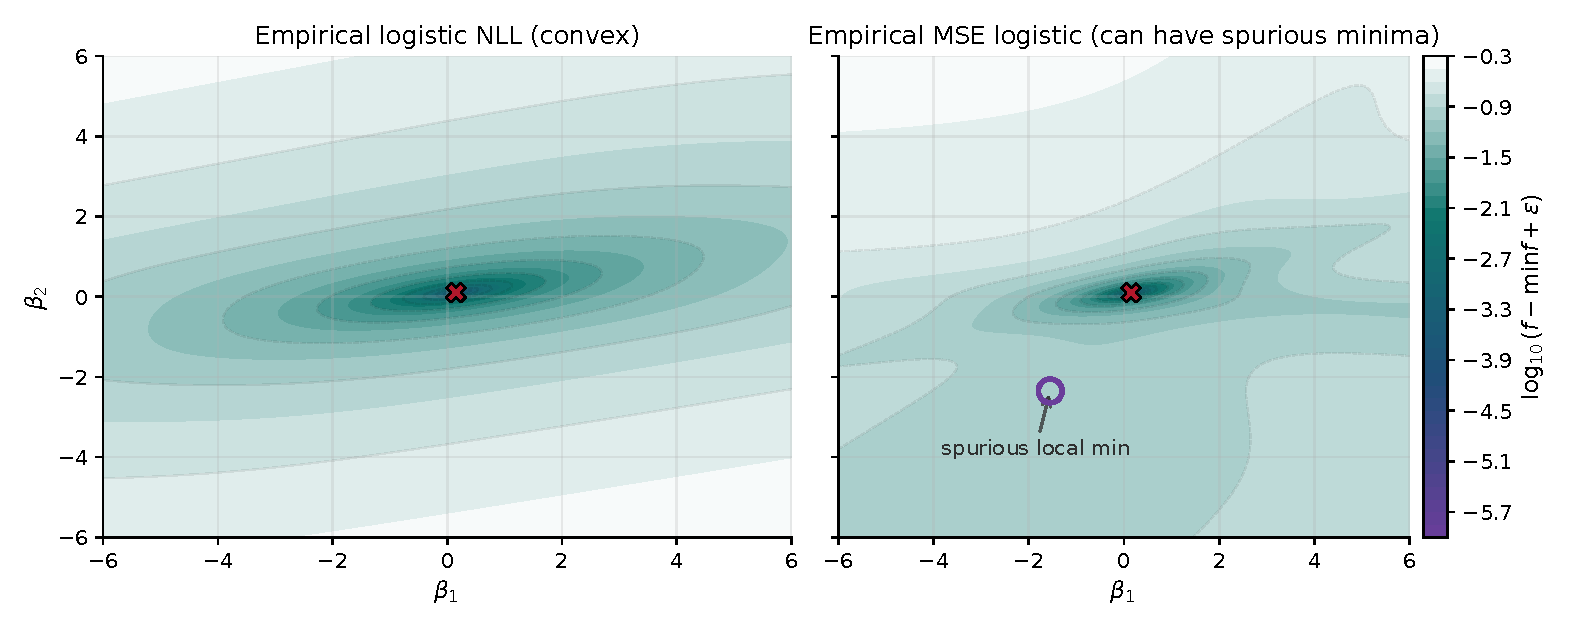
\includegraphics[width=\textwidth]{figures/handouts/convexity_optimization/fig_logistic_empirical_spurious}
  \caption{Empirical logistic landscapes on the dataset in \Cref{ex:logistic-empirical-spurious}.
  The plots show $\log_{10}(f-\min f+\varepsilon)$ for each objective.
  The red X marks the global minimizer in each panel.
  Left: the NLL is convex (one basin).
  Right: the squared-loss objective can have a spurious local minimum (circled), so a local method can get stuck.}
  \label{fig:logistic-empirical-spurious}
\end{figure}

\begin{figure}[t]
  \centering
  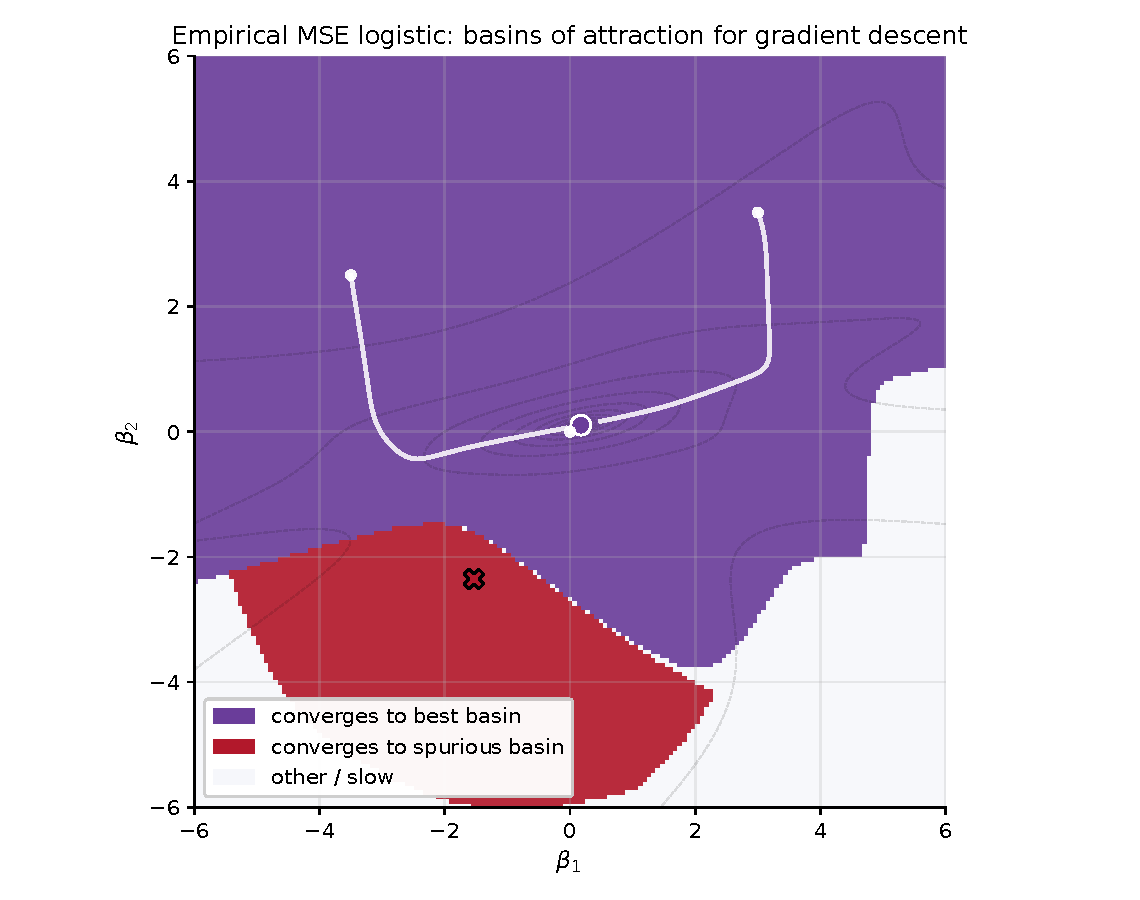
\includegraphics[width=0.92\textwidth]{figures/handouts/convexity_optimization/fig_logistic_empirical_basins}
  \caption{Basins of attraction for gradient descent on the empirical MSE-logistic objective in \Cref{ex:logistic-empirical-spurious}.
  The purple dot and red X mark the two local minimizers.
  Each initialization is colored by which local minimizer fixed-step GD (with $\eta=0.6$) converges to, and the overlaid paths show a few representative trajectories.}
  \label{fig:logistic-empirical-basins}
\end{figure}

Now assume a realizable population model:
\[
Y\mid X=x \sim \mathrm{Bernoulli}(p^\star(x)),
\qquad
p^\star(x) = \sigma(x^\top\beta^\star).
\]
Then the expected squared loss decomposes as
\[
\E\big[(Y-\sigma(X^\top\beta))^2\mid X\big]
= p^\star(X)(1-p^\star(X)) + \big(p^\star(X)-\sigma(X^\top\beta)\big)^2,
\]
so (up to an additive constant) the population objective becomes
\begin{equation}
R(\beta) = \E\big[(\sigma(X^\top\beta)-\sigma(X^\top\beta^\star))^2\big].
\label{eq:logistic-pop-risk}
\end{equation}

\begin{proposition}[One-point monotonicity in the realizable population squared-loss risk]
\label{prop:logistic-pop-one-point}
Assume $\E[\norm{X}_2]<\infty$, and let $R$ be as in \eqref{eq:logistic-pop-risk}. Then for all $\beta$,
\begin{equation}
\ip{\nabla R(\beta)}{\beta-\beta^\star} \ge 0.
\label{eq:one-point}
\end{equation}
In particular, along any ray $\beta(t)=\beta^\star+t(\beta-\beta^\star)$, the function $t\mapsto R(\beta(t))$ is nondecreasing for $t\ge 0$.
\end{proposition}

The next exercise isolates the population monotonicity calculation; structurally it plays the same role as the first-order convexity arguments in the Optimization unit.
\begin{exercise}[One-point monotonicity for realizable MSE-logistic]
\label{ex:logistic-one-point}
Prove \Cref{prop:logistic-pop-one-point}.
Let $\eta=X^\top\beta$ and $\eta^\star=X^\top\beta^\star$.
\begin{enumerate}[leftmargin=*]
  \item Differentiate under the expectation in \eqref{eq:logistic-pop-risk} to show that
  \[
  \nabla R(\beta)
  =2\,\E\Big[(\sigma(\eta)-\sigma(\eta^\star))\,\sigma'(\eta)\,X\Big].
  \]
  \item Show that
  \[
  \ip{\nabla R(\beta)}{\beta-\beta^\star}
  =2\,\E\Big[\sigma'(\eta)\,(\sigma(\eta)-\sigma(\eta^\star))(\eta-\eta^\star)\Big],
  \]
  and conclude it is nonnegative using only that $\sigma$ is increasing and $\sigma'\ge 0$.
  \item Deduce the ray-monotonicity statement by differentiating $g(t)=R(\beta^\star+t(\beta-\beta^\star))$.
\end{enumerate}
\end{exercise}

\SolutionBox[14]{%
\emph{Part (1).}
Differentiate \eqref{eq:logistic-pop-risk} under the expectation:
\[
R(\beta)=\E\big[(\sigma(X^\top\beta)-\sigma(X^\top\beta^\star))^2\big].
\]
Using the chain rule, $\nabla_\beta\sigma(X^\top\beta)=\sigma'(X^\top\beta)\,X$, hence
\[
\nabla R(\beta)
=2\,\E\Big[(\sigma(\eta)-\sigma(\eta^\star))\,\sigma'(\eta)\,X\Big],
\qquad
\eta=X^\top\beta,\ \eta^\star=X^\top\beta^\star.
\]

\emph{Part (2).}
Take the inner product with $(\beta-\beta^\star)$ and use $\ip{X}{\beta-\beta^\star}=\eta-\eta^\star$:
\[
\ip{\nabla R(\beta)}{\beta-\beta^\star}
=2\,\E\Big[\sigma'(\eta)\,(\sigma(\eta)-\sigma(\eta^\star))(\eta-\eta^\star)\Big].
\]
Since $\sigma'(\eta)\ge 0$ and $\sigma$ is increasing, we have
$(\sigma(\eta)-\sigma(\eta^\star))(\eta-\eta^\star)\ge 0$ pointwise.
Therefore the integrand is pointwise nonnegative, and the expectation is nonnegative as claimed.

\emph{Part (3) (ray monotonicity).}
For the ray $\beta(t)=\beta^\star+t(\beta-\beta^\star)$, define $g(t)=R(\beta(t))$.
By the chain rule,
\[
g'(t)=\ip{\nabla R(\beta(t))}{\beta-\beta^\star}\ge 0,
\]
so $t\mapsto R(\beta(t))$ is nondecreasing for $t\ge 0$.
(The argument uses only that the link is increasing with nonnegative derivative, so it holds for any such link function.)%
}

\begin{corollary}[Realizable population MSE-logistic has no spurious local minima]
\label{cor:logistic-pop-no-spurious}
Under the assumptions of \Cref{prop:logistic-pop-one-point}, every local minimizer of the realizable population risk $R$ in \eqref{eq:logistic-pop-risk} is global.
If in addition $\E[XX^\top]\succ 0$, then the unique global minimizer is $\beta^\star$.
\end{corollary}

\begin{exercise}[Stationarity + one-point monotonicity $\Rightarrow$ no spurious local minima]
\label{ex:logistic-one-point-no-spurious}
Prove \Cref{cor:logistic-pop-no-spurious} from \Cref{prop:logistic-pop-one-point}.
\begin{enumerate}[leftmargin=*]
  \item Let $\bar\beta$ be a local minimizer. Since $R$ is differentiable, $\nabla R(\bar\beta)=0$.
  Combine this with \Cref{eq:one-point} to show that
  \[
    0
    = \ip{\nabla R(\bar\beta)}{\bar\beta-\beta^\star}
    = 2\,\E\Big[\sigma'(\bar\eta)\,(\sigma(\bar\eta)-\sigma(\eta^\star))(\bar\eta-\eta^\star)\Big],
  \]
  where $\bar\eta=X^\top\bar\beta$ and $\eta^\star=X^\top\beta^\star$.
  Conclude that $\sigma(X^\top\bar\beta)=\sigma(X^\top\beta^\star)$ almost surely.
  \item Deduce that $R(\bar\beta)=0$, so $\bar\beta$ is a global minimizer.
  \item For uniqueness: show that if $R(\beta)=0$, then $X^\top(\beta-\beta^\star)=0$ almost surely, and deduce $\beta=\beta^\star$ under $\E[XX^\top]\succ 0$.
\end{enumerate}
\end{exercise}

\SolutionBox[14]{%
\emph{Part (1).}
Let $\bar\beta$ be a local minimizer of the differentiable function $R$.
Then $\nabla R(\bar\beta)=0$.
Applying \Cref{prop:logistic-pop-one-point} at $\beta=\bar\beta$ gives
\[
0
= \ip{\nabla R(\bar\beta)}{\bar\beta-\beta^\star}
= 2\,\E\Big[\sigma'(\bar\eta)\,(\sigma(\bar\eta)-\sigma(\eta^\star))(\bar\eta-\eta^\star)\Big],
\qquad \bar\eta=X^\top\bar\beta,\ \eta^\star=X^\top\beta^\star.
\]
The integrand is pointwise nonnegative because $\sigma'(\bar\eta)\ge 0$ and $\sigma$ is increasing, so the expectation can vanish only if the integrand is zero almost surely.
Since $\sigma'(z)>0$ for every finite $z$, this implies
\[
(\sigma(\bar\eta)-\sigma(\eta^\star))(\bar\eta-\eta^\star)=0
\qquad\text{almost surely.}
\]
Because $\sigma$ is strictly increasing, the product above is zero if and only if $\bar\eta=\eta^\star$, equivalently $\sigma(X^\top\bar\beta)=\sigma(X^\top\beta^\star)$ almost surely.

\emph{Part (2).}
If $\sigma(X^\top\bar\beta)=\sigma(X^\top\beta^\star)$ almost surely, then the integrand in \eqref{eq:logistic-pop-risk} vanishes almost surely, so
\[
R(\bar\beta)=\E\big[(\sigma(X^\top\bar\beta)-\sigma(X^\top\beta^\star))^2\big]=0.
\]
Since $R(\beta^\star)=0$ as well, $\bar\beta$ is a global minimizer.

\emph{Part (3) (uniqueness).}
If $R(\beta)=0$, then
\[
\E\big[(\sigma(X^\top\beta)-\sigma(X^\top\beta^\star))^2\big]=0,
\]
so $\sigma(X^\top\beta)=\sigma(X^\top\beta^\star)$ almost surely.
Since $\sigma$ is strictly increasing, this implies $X^\top(\beta-\beta^\star)=0$ almost surely.
Taking expectations yields
$(\beta-\beta^\star)^\top\E[XX^\top](\beta-\beta^\star)=0$.
If $\E[XX^\top]\succ 0$, then the quadratic form is strictly positive unless $\beta=\beta^\star$, so $\beta^\star$ is the unique global minimizer.%
}

The population MSE-logistic risk is nonconvex, but it still has the simple geometry that moving away from $\beta^\star$ does not help along any ray from $\beta^\star$.
This is qualitatively different from objectives like ecological logistic regression (\Cref{sec:ecological-logistic}), where aggregation introduces intrinsic nonconvexity and the landscape can have many distinct basins even under a clean population model.

Even with this benign global geometry, gradient descent can be slow because of saturation and flat plateaus.
The one-point monotonicity in \Cref{prop:logistic-pop-one-point} is a global geometry guarantee, but it is not a rate guarantee.
Far from $\beta^\star$, the squared-loss logistic objective can become very flat because the logistic link saturates:
$\sigma(z)\to 0$ or $1$ and $\sigma'(z)\to 0$ as $|z|\to\infty$.
The squared-loss gradient carries a factor of $\sigma'(X^\top\beta)$, so when the model is very confident (large $|X^\top\beta|$), the gradient can be tiny even if the objective value is not close to its minimum.
This mirrors the ``confidence weights'' story for convex NLL objectives:
in logistic NLL, curvature is largest near the decision boundary, while very confident points contribute little.
For squared loss, that same saturation suppresses the \emph{descent signal} itself, producing plateaus where $\norm{\nabla R(\beta)}_2$ is small even though $R(\beta)-R(\beta^\star)$ is not.

\begin{proposition}[Realizable squared-loss logistic: arbitrarily flat far from $\beta^\star$]
\label{prop:logistic-pop-flat}
Assume $\E[\norm{X}_2]<\infty$ and let $R$ be the realizable population risk \eqref{eq:logistic-pop-risk}.
Define $g(t)=R(t\beta^\star)$ for $t\ge 1$.
Then:
\begin{enumerate}[leftmargin=*]
  \item $g$ is nondecreasing on $[1,\infty)$ and converges to a finite limit $g(\infty)$.
  \item $\lim_{t\to\infty} g'(t)=0$ and $\lim_{t\to\infty}\norm{\nabla R(t\beta^\star)}_2=0$.
  \item If $\Pr(X^\top\beta^\star\neq 0)>0$, then $g(\infty)>0$.
\end{enumerate}
In particular, there are directions along which the landscape becomes arbitrarily flat even though the excess risk stays bounded away from $0$.
\end{proposition}

\emph{Proof idea.} See Exercise~\ref{ex:logistic-plateau}.

\begin{exercise}[Prove the plateau]
\label{ex:logistic-plateau}
In the realizable population model, let $g(t)=R(t\beta^\star)$ for $t\ge 1$.
\begin{enumerate}[leftmargin=*]
  \item Show that
  \[
    g'(t)=2\,\E\big[(\sigma(t\eta^\star)-\sigma(\eta^\star))\,\sigma'(t\eta^\star)\,\eta^\star\big],
    \qquad \eta^\star=X^\top\beta^\star,
  \]
  and conclude that $g$ is nondecreasing (hence $g(t)\to g(\infty)$ since $0\le g(t)\le 1$).
  \item Show that $g'(t)\to 0$ and $\nabla R(t\beta^\star)\to 0$ as $t\to\infty$.
  Interpret this as: \emph{without} a PL/strong-convexity-type condition, small gradient does not imply near-optimality.
  \item Assume $\Pr(\eta^\star\neq 0)>0$.
  Show that $g(\infty)>0$.
\end{enumerate}
\end{exercise}

\SolutionBox[12]{%
Write $\eta^\star=X^\top\beta^\star$ so that $g(t)=\E[(\sigma(t\eta^\star)-\sigma(\eta^\star))^2]$.

\emph{Part (1).}
Differentiate under the expectation:
by the chain rule,
\[
\frac{d}{dt}\sigma(t\eta^\star)=\sigma'(t\eta^\star)\,\eta^\star,
\]
so
\[
g'(t)
=\E\Big[2(\sigma(t\eta^\star)-\sigma(\eta^\star))\cdot \sigma'(t\eta^\star)\,\eta^\star\Big]
=2\,\E\big[(\sigma(t\eta^\star)-\sigma(\eta^\star))\,\sigma'(t\eta^\star)\,\eta^\star\big].
\]
For $t\ge 1$, $\sigma(t\eta^\star)-\sigma(\eta^\star)$ has the same sign as $(t-1)\eta^\star$ since $\sigma$ is increasing.
Because $\sigma'\ge 0$, the integrand is pointwise nonnegative, hence $g'(t)\ge 0$ and $g$ is nondecreasing.
Since $g(t)\in[0,1]$, it follows that $g(t)\to g(\infty)$ for some finite limit $g(\infty)$.

\emph{Part (2).}
For each fixed $\eta^\star\neq 0$, we have $t\eta^\star\to \pm\infty$ and therefore $\sigma'(t\eta^\star)\to 0$ as $t\to\infty$.
Also,
\[
\big|(\sigma(t\eta^\star)-\sigma(\eta^\star))\,\sigma'(t\eta^\star)\,\eta^\star\big|
\le \sigma'(0)\,|\eta^\star|
\le \sigma'(0)\,\norm{\beta^\star}_2\,\norm{X}_2,
\]
which is integrable since $\E[\norm{X}_2]<\infty$.
We will use the following standard fact: if random variables $Z_t$ satisfy $|Z_t|\le W$ with $\E[W]<\infty$ and $Z_t\to 0$ almost surely, then $\E[Z_t]\to 0$.
Applying this fact here gives $g'(t)\to 0$ as $t\to\infty$.

\smallskip
Similarly, differentiating \eqref{eq:logistic-pop-risk} gives
\[
\nabla R(t\beta^\star)
=2\,\E\big[(\sigma(t\eta^\star)-\sigma(\eta^\star))\,\sigma'(t\eta^\star)\,X\big].
\]
The integrand norm is bounded by $2\sigma'(0)\norm{X}_2$, and for each fixed $X$ the factor $\sigma'(t\eta^\star)$ tends to $0$ (or the bracketed term vanishes when $\eta^\star=0$), so the same reasoning lets us pass the limit through the expectation and conclude $\nabla R(t\beta^\star)\to 0$.

\emph{Part (3).}
As $t\to\infty$ we have $\sigma(t\eta^\star)\to 1$ when $\eta^\star>0$, $\sigma(t\eta^\star)\to 0$ when $\eta^\star<0$, and $\sigma(t\eta^\star)=\sigma(\eta^\star)=1/2$ when $\eta^\star=0$.
Since $0\le (\sigma(t\eta^\star)-\sigma(\eta^\star))^2\le 1$, we can apply the same fact (with $W=1$) to pass the limit through the expectation and obtain
\[
g(\infty)=\E\Big[(1-\sigma(\eta^\star))^2\mathbf{1}\{\eta^\star>0\} + \sigma(\eta^\star)^2\mathbf{1}\{\eta^\star<0\}\Big].
\]
If $\Pr(\eta^\star\neq 0)>0$, then the integrand is strictly positive on $\{\eta^\star\neq 0\}$, so $g(\infty)>0$.

Along this ray, the risk can remain bounded away from $0$ while the gradient (and directional derivative) goes to $0$.
Without a condition like PL/strong convexity, a small gradient does not by itself certify near-optimality.
}

Conditions like strong convexity or the PL inequality (\Cref{def:pl-inequality}) prevent this phenomenon: they rule out large flat regions away from the optimum by relating gradient size to suboptimality.
\Cref{prop:logistic-pop-flat} shows the realizable squared-loss logistic risk does not have such a global guarantee in general.

In the realizable population model, the one-point monotonicity in \Cref{prop:logistic-pop-one-point} is a \emph{global} geometric statement.
To get an actual rate for gradient descent, we also need a \emph{local curvature} condition near $\beta^\star$.
One simple sufficient condition is bounded features, which implies local strong convexity (hence a linear rate) around the optimum.

\begin{proposition}[Local linear convergence of gradient descent near $\beta^\star$]
\label{prop:logistic-pop-local-rate}
Assume $\E[XX^\top]\succeq \lambda I_d$ and $\norm{X}_2\le R$ almost surely for some $\lambda,R>0$.
Then at $\beta^\star$,
\[
\Hess R(\beta^\star)\succeq m_0 I_d,
\qquad
m_0 = 2\,\sigma'(R\norm{\beta^\star}_2)^2\,\lambda,
\]
and there exist $r>0$ and constants $0<m\le L<\infty$ such that the population risk $R$ in \eqref{eq:logistic-pop-risk} is $m$-strongly convex and $L$-smooth on the ball $\{\beta:\ \norm{\beta-\beta^\star}_2\le r\}$.
Consequently, gradient descent with step size $1/L$ initialized in this ball satisfies
\[
R(\beta^{(k)})-R(\beta^\star)
\le \left(1-\frac{m}{L}\right)^k\bigl(R(\beta^{(0)})-R(\beta^\star)\bigr)
\qquad\text{(see \citealp[\S9.3]{boyd_vandenberghe_2004_convex}).}
\]
\end{proposition}

\begin{proof}
Differentiate \eqref{eq:logistic-pop-risk} twice.
At $\beta=\beta^\star$, the cross term vanishes and the Hessian simplifies to
\[
\Hess R(\beta^\star)=2\,\E\big[\sigma'(X^\top\beta^\star)^2\,XX^\top\big].
\]
Since $\norm{X^\top\beta^\star}\le \norm{X}_2\norm{\beta^\star}_2\le R\norm{\beta^\star}_2$ almost surely, we have
$\sigma'(X^\top\beta^\star)\ge \sigma'(R\norm{\beta^\star}_2)>0$ almost surely (since $\sigma'$ is even and decreases with $|z|$), hence
\[
\Hess R(\beta^\star)\succeq 2\,\sigma'(R\norm{\beta^\star}_2)^2\,\E[XX^\top]\succeq 2\,\sigma'(R\norm{\beta^\star}_2)^2\,\lambda I_d.
\]
This is the claimed bound with $m_0=2\,\sigma'(R\norm{\beta^\star}_2)^2\,\lambda$.
Because $R$ is twice continuously differentiable and $\norm{X}_2\le R$ almost surely, $\Hess R(\beta)$ varies continuously in $\beta$ and is bounded on compact sets.
Therefore, on a sufficiently small ball around $\beta^\star$, the Hessian is bounded below by (say) $\tfrac12 m_0 I_d$ and above by $L I_d$ for some finite $L$, which gives local strong convexity and smoothness.
The linear convergence rate for gradient descent on an $m$-strongly convex and $L$-smooth function is standard (cited above).
\end{proof}

Under misspecification, hard multimodality can return.
If $p^\star(x)$ is not representable as $\sigma(x^\top\beta)$ (e.g.\ marginalizing over latent classes can yield mixtures of logits), then \eqref{eq:one-point} need not hold, and the population squared-loss risk can become bimodal with spurious local minima.
Benign global geometry often hinges on model and data assumptions.
This is one reason MLE (convex NLL) is often more stable than squared-loss fitting in logistic-type binary regression models.

\begin{example}[Misspecification can create a spurious local minimum for squared-loss logistic regression]
\label{ex:logistic-misspecified-spurious}
Consider a 1D feature $X$ that takes values $\{-2,-1,1,2\}$ with equal probability, and parameterize $\beta=(\beta_0,\beta_1)$ so that $q_\beta(x)=\sigma(\beta_0+\beta_1 x)$.
Let the true conditional probabilities be
\[
p^\star(-2)=0.49,\quad p^\star(-1)=0.87,\quad p^\star(1)=0.92,\quad p^\star(2)=0.36.
\]
This $p^\star$ is not representable as $q_\beta$, since it is not monotone in $x$.

For the population squared-loss risk $R_{\mathrm{MSE}}(\beta)=\E[(q_\beta(X)-p^\star(X))^2]$, a direct evaluation shows two distinct basins:
numerically, evaluating $R_{\mathrm{MSE}}$ on a grid reveals a global minimizer and a spurious local minimizer.
See \Cref{fig:logistic-landscape-2d}.
\end{example}

\begin{figure}[t]
  \centering
  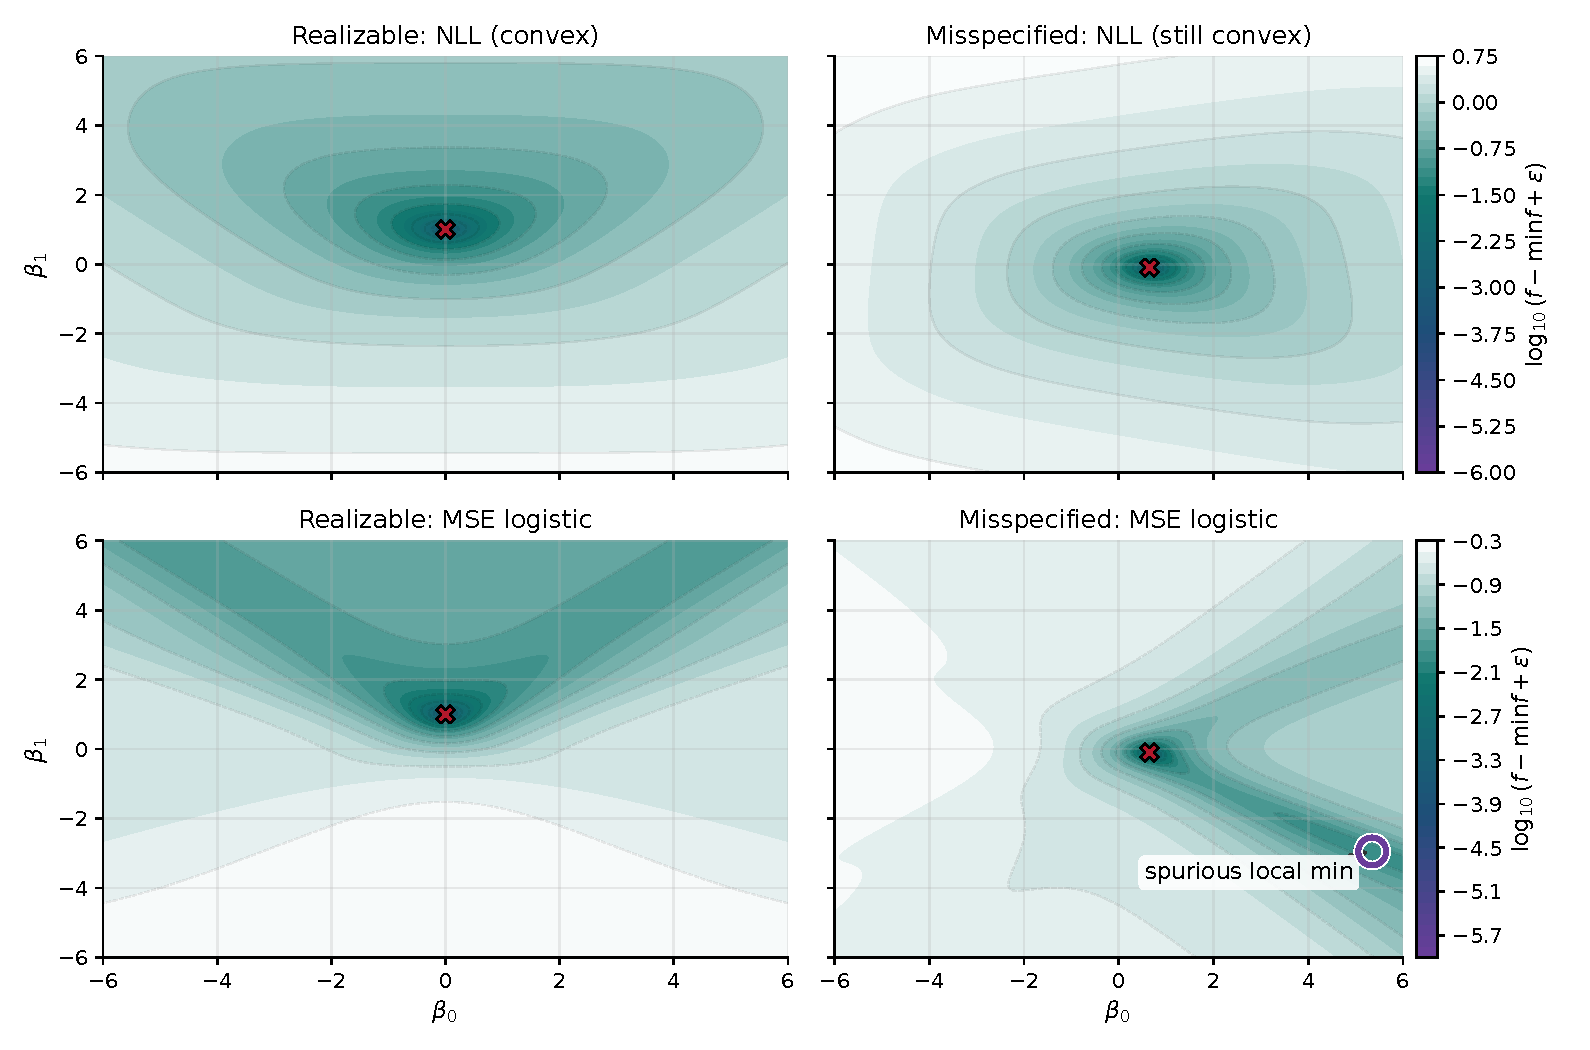
\includegraphics[width=\textwidth]{figures/handouts/convexity_optimization/fig_logistic_landscape_2d}
  \caption{A consistent contourf view of logistic landscapes in a 2D parameterization $\beta=(\beta_0,\beta_1)$.
  The plots show $\log_{10}(f-\min f+\varepsilon)$ for each objective, which makes basins comparable across panels.
  The red X marker indicates the global minimizer in each panel; in the bottom-right plot, the circled point is a spurious local minimum.
  In this example, the NLL landscape is unimodal in both realizable and misspecified settings, while the squared-loss landscape can develop extra basins under misspecification.}
  \label{fig:logistic-landscape-2d}
\end{figure}

% ------------------------------------------------------------
Example~I separates three distinct regimes.
Empirical MSE-logistic can create spurious basins; the realizable population risk has no spurious local minima but can still be slow because of broad plateaus; and misspecification can bring back genuinely wrong stable basins.
The response depends on the regime: use a stable objective when possible, use damping or line search when curvature is unreliable, and use restarts or stronger initializations when multiple basins are present.

% ------------------------------------------------------------
\section[Example II (phase retrieval)]{Example II: multimodality from symmetry, but only global optima in phase retrieval}
\label{sec:phase-retrieval}

In coherent diffraction imaging, optics, and astronomy, sensors measure intensities and lose phase.
A canonical real model is \emph{phase retrieval}:
\[
y_i = (a_i^\top x^\star)^2,\qquad i=1,\dots,m,
\]
where $x^\star\in\R^d$ is the unknown signal and $a_i$ are known sensing vectors.
A standard nonconvex least-squares objective is
\begin{equation}
F(x)=\frac{1}{4m}\sum_{i=1}^m\big((a_i^\top x)^2 - y_i\big)^2.
\label{eq:phase-empirical}
\end{equation}
This objective is nonconvex for structural reasons (it involves squares of linear forms),
and it is \emph{inherently} multimodal because $x^\star$ and $-x^\star$ generate the same data.

Like squared-loss logistic regression, phase retrieval is a smooth, nonconvex least-squares objective.
But here the nonconvexity is driven primarily by a \emph{symmetry}: $x^\star$ and $-x^\star$ generate the same data.
In population (for Gaussian designs), this symmetry produces multiple global optima but \emph{no} suboptimal local minima; the remaining stationary points are saddles.
This is ``benign'' nonconvexity (a strict-saddle picture), and it contrasts with ecological logistic regression (\Cref{sec:ecological-logistic}), where aggregation creates intrinsic nonconvexity and can lead to many distinct basins.
This ``benign geometry'' picture (multiple equivalent global minimizers; strict saddles elsewhere) appears broadly in modern tractable nonconvex problems; see \citet[\S2]{sun_qu_wright_2015_nonconvex_not_scary} and \citet[\S1]{zhang_qu_wright_2020_symmetry_geometry}.

\begin{figure}[t]
  \centering
  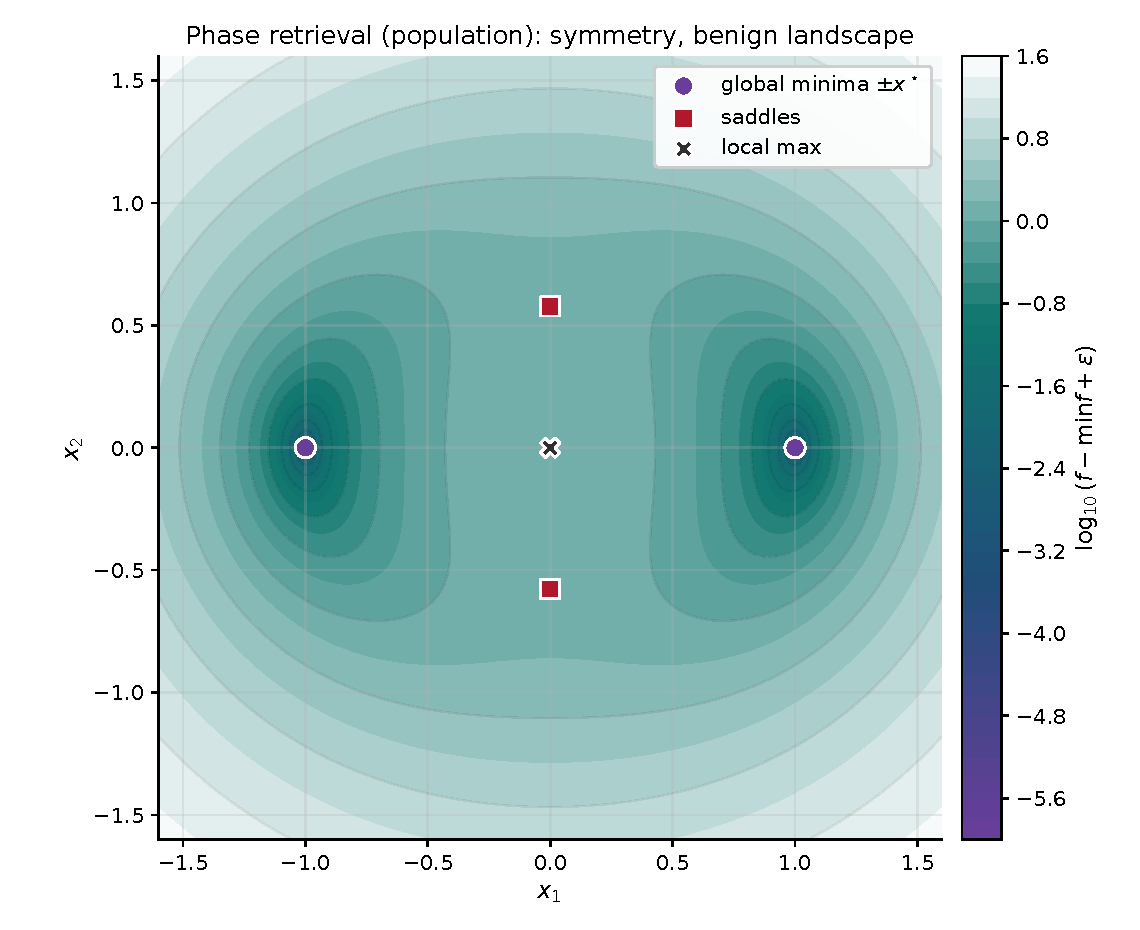
\includegraphics[width=0.86\textwidth]{figures/handouts/convexity_optimization/fig_phase_retrieval_landscape}
  \caption{Population phase retrieval in $d=2$: the landscape is nonconvex and symmetric ($x\sim -x$), but the only local minima are the two global minima $\pm x^\star$; other critical points are saddles or a local maximum at the origin.}
  \label{fig:phase-retrieval-landscape}
\end{figure}

For a clean population model, assume $a\sim N(0,I_d)$ and consider the \emph{population} objective
\begin{equation}
  f(x)=\frac12\,\E\Big[\big((a^\top x)^2 - (a^\top x^\star)^2\big)^2\Big].
  \label{eq:phase-pop}
\end{equation}

\begin{proposition}[Population phase retrieval: nonconvex but no spurious local minima]
\label{prop:phase-retrieval-benign}
For $f$ in \eqref{eq:phase-pop},
\begin{equation}
  f(x)
  =\frac{3}{2}\norm{x}^4 - \norm{x}^2\norm{x^\star}^2 - 2\ip{x}{x^\star}^2 + \frac{3}{2}\norm{x^\star}^4,
  \label{eq:phase-pop-closed-form}
\end{equation}
and the stationary points are:
\begin{enumerate}[leftmargin=*]
  \item global minima $x=\pm x^\star$ (value $0$),
  \item a local maximum at $x=0$,
  \item a saddle set $\{x:\ x\perp x^\star,\ \norm{x}=\norm{x^\star}/\sqrt{3}\}$.
\end{enumerate}
In particular, every local minimum is global.
\end{proposition}

\begin{exercise}[Phase retrieval: derive and classify the population stationary points]
\label{ex:phase-pop-derivation}
Prove \Cref{prop:phase-retrieval-benign}.
\begin{enumerate}[leftmargin=*]
  \item Expand \eqref{eq:phase-pop} and use the Gaussian fourth-moment identities
  \[
  \E[(a^\top u)^4]=3\norm{u}^4,
  \qquad
  \E[(a^\top u)^2(a^\top v)^2]=\norm{u}^2\norm{v}^2 + 2\ip{u}{v}^2,
  \]
  to obtain \eqref{eq:phase-pop-closed-form}.
  \item Differentiate \eqref{eq:phase-pop-closed-form} to get an explicit formula for $\nabla f(x)$.
  \item Solve $\nabla f(x)=0$ by decomposing $x=\alpha x^\star + u$ with $u\perp x^\star$.
  \item Classify the stationary points as global minima, a local maximum, and a saddle set.
\end{enumerate}
\end{exercise}

\SolutionBox[22]{%
\emph{Part (1) (closed form).}
Expanding the square in \eqref{eq:phase-pop} gives
\[
f(x)
=\frac12\,\E\big[(a^\top x)^4\big]
\;-\;\E\big[(a^\top x)^2(a^\top x^\star)^2\big]
\;+\;\frac12\,\E\big[(a^\top x^\star)^4\big].
\]
Apply the stated Gaussian fourth-moment identities with $u=x$ and $v=x^\star$ to get
\[
\E[(a^\top x)^4]=3\norm{x}^4,\qquad
\E[(a^\top x^\star)^4]=3\norm{x^\star}^4,
\]
and
\[
\E[(a^\top x)^2(a^\top x^\star)^2]=\norm{x}^2\norm{x^\star}^2 + 2\ip{x}{x^\star}^2.
\]
Substituting yields \eqref{eq:phase-pop-closed-form}.

\emph{Part (2) (gradient).}
Differentiate \eqref{eq:phase-pop-closed-form}:
\[
\nabla f(x)
= 6\norm{x}^2 x - 2\norm{x^\star}^2 x - 4\ip{x}{x^\star}x^\star
= (6\norm{x}^2-2\norm{x^\star}^2)x - 4\ip{x}{x^\star}x^\star.
\]

\emph{Part (3) (stationary points).}
Let $r=\norm{x^\star}_2$ and decompose $x=\alpha x^\star + u$ with $u\perp x^\star$.
Then $\ip{x}{x^\star}=\alpha r^2$ and $\norm{x}^2=\alpha^2r^2+\norm{u}^2$.
Setting $\nabla f(x)=0$ and matching the $u$ and $x^\star$ components gives
\[
(6\norm{x}^2-2r^2)\,u=0,
\qquad
\alpha\,(6\norm{x}^2-6r^2)=0.
\]
If $u=0$, then either $\alpha=0$ (so $x=0$) or $\norm{x}^2=r^2$ (so $\alpha=\pm 1$ and $x=\pm x^\star$).
If $u\neq 0$, then the first equation forces $\norm{x}^2=r^2/3$, and the second forces $\alpha=0$, hence
$x\perp x^\star$ and $\norm{x}=r/\sqrt{3}$.
This gives exactly the stationary-point list in \Cref{prop:phase-retrieval-benign}.

\emph{Part (4) (classification).}
Since $f$ in \eqref{eq:phase-pop} is an expectation of a square, $f(x)\ge 0$ for all $x$.
Also $f(\pm x^\star)=0$, so $\pm x^\star$ are global minima.

For $x=0$, the expansion \eqref{eq:phase-pop-closed-form} shows
\[
f(0)-f(x)= r^2\norm{x}^2 + 2\ip{x}{x^\star}^2 - \frac{3}{2}\norm{x}^4,
\]
which is strictly positive for all sufficiently small $x\neq 0$ (the quadratic term dominates), so $x=0$ is a local maximum.

Finally, if $x\perp x^\star$ and $\norm{x}=r/\sqrt{3}$, then the univariate restriction $t\mapsto f(x+t x^\star)$ has negative second derivative at $t=0$, so there is a direction of negative curvature.
Hence these points are saddles, and every local minimum is global.%
}

This is symmetry-driven nonconvexity with a strict-saddle geometry:
every non-optimal stationary point has a direction of negative curvature.

Phase retrieval is typically approached via the two-stage template in \Cref{alg:two-stage-template}:
use a cheap global initializer, then run a local method.
In the Gaussian model, there is a clean way to build a provably good direction estimate from a simple moment identity.
Assume the noiseless Gaussian design model $a_i \stackrel{\mathrm{iid}}{\sim} N(0,I_d)$ with measurements $y_i=(a_i^\top x^\star)^2$.
Define the \emph{spectral matrix}
\[
  Y = \frac{1}{m}\sum_{i=1}^m y_i a_i a_i^\top.
\]
Also define the radius estimate
\[
  \hat r^2 = \frac{1}{m}\sum_{i=1}^m y_i,
\]
which satisfies $\E[\hat r^2]=\norm{x^\star}_2^2$.
If $\hat u$ is a unit-norm top eigenvector of $Y$, then the standard spectral initializer is $x^{(0)}=\hat r\,\hat u$.

The next proposition explains why this initialization is reasonable.
It shows that (i) the population matrix $\E[Y]$ has a unique leading eigenvector in the $x^\star$ direction, and (ii) if the empirical $Y$ is close to $\E[Y]$ in operator norm then its leading eigenvector must be close to $\pm x^\star/\norm{x^\star}_2$.
(Here $\norm{M}_{\mathrm{op}}$ denotes the operator norm, i.e.\ the largest absolute eigenvalue for a symmetric matrix $M$.)

\begin{proposition}[Gaussian phase retrieval: why the spectral initializer points at $x^\star$]
\label{prop:phase-spectral-init}
Assume $x^\star\neq 0$, let $a\sim N(0,I_d)$, and set $y=(a^\top x^\star)^2$.
Write $r=\norm{x^\star}_2$ and $u^\star=x^\star/r$.
Define the population matrix
\[
  Y_{\mathrm{pop}} = \E\big[y\,a a^\top\big]
  = \E\big[(a^\top x^\star)^2 a a^\top\big].
\]
Then
\[
  Y_{\mathrm{pop}}=r^2 I_d + 2x^\star(x^\star)^\top,
\]
so the unique leading eigenvector of $Y_{\mathrm{pop}}$ is $u^\star$.
Moreover, if $Y$ is any symmetric matrix satisfying
\[
\norm{Y-Y_{\mathrm{pop}}}_{\mathrm{op}} \le \varepsilon\, r^2
\qquad\text{for some }\varepsilon\in(0,1),
\]
then for every unit-norm leading eigenvector $\hat u$ of $Y$ there exists a sign $s\in\{\pm 1\}$ such that
$\norm{\hat u-su^\star}_2\le \sqrt{2\varepsilon}$.
\end{proposition}

\begin{exercise}[Phase retrieval: why spectral initialization points at $x^\star$]
\label{ex:phase-spectral-spike}
Prove \Cref{prop:phase-spectral-init}.
Conclude that if the empirical matrix $Y$ is close to $Y_{\mathrm{pop}}$ in operator norm, then its top eigenvector is close to $\pm u^\star$ and the spectral initializer $x^{(0)}=\hat r\,\hat u$ is close to $\pm x^\star$.
\emph{Hint:} to compute $Y_{\mathrm{pop}}$, you can either compute entries using the Gaussian fourth-moment identity
$\E[a_i a_j a_k a_\ell]=\delta_{ij}\delta_{k\ell}+\delta_{ik}\delta_{j\ell}+\delta_{i\ell}\delta_{jk}$,
or compute the entries directly by expanding.
For the perturbation bound, compare quadratic forms $v^\top Y v$ and use $|v^\top (Y-Y_{\mathrm{pop}}) v|\le \norm{Y-Y_{\mathrm{pop}}}_{\mathrm{op}}$ for unit $v$.
Finally, explain in a sentence why one expects $\norm{Y-Y_{\mathrm{pop}}}_{\mathrm{op}}$ to be small when $m$ is large in the Gaussian model.
\end{exercise}

\SolutionBox[20]{%
Write $u=x^\star$ and expand $y=(a^\top u)^2=\sum_{k,\ell} u_k u_\ell a_k a_\ell$.
For each entry $(i,j)$,
\[
\E\!\big[y\,a_i a_j\big]
=\sum_{k,\ell} u_k u_\ell\,\E[a_i a_j a_k a_\ell]
=\sum_{k,\ell} u_k u_\ell\bigl(\delta_{ij}\delta_{k\ell}+\delta_{ik}\delta_{j\ell}+\delta_{i\ell}\delta_{jk}\bigr).
\]
The first term gives $\delta_{ij}\sum_k u_k^2=\delta_{ij}\norm{u}_2^2$.
The second and third terms each give $u_i u_j$.
Thus $\E[y\,a_i a_j]=\norm{u}_2^2\,\delta_{ij}+2u_i u_j$, i.e.
$Y_{\mathrm{pop}}=\norm{u}_2^2 I_d + 2uu^\top$.

For eigenvalues, note that $Y_{\mathrm{pop}}u=(\norm{u}_2^2+2\norm{u}_2^2)u=3\norm{u}_2^2 u$.
If $w\perp u$, then $uu^\top w=0$ so $Y_{\mathrm{pop}}w=\norm{u}_2^2 w$.
Hence the unique top eigenspace is $\mathrm{span}\{u\}$.

Let $r=\norm{u}_2$ and $u^\star=u/r$.
Let $\hat u$ be a unit top eigenvector of $Y$.
Write $E=Y-Y_{\mathrm{pop}}$ and assume $\norm{E}_{\mathrm{op}}\le \varepsilon r^2$.
Then
\[
\hat u^\top Y_{\mathrm{pop}} \hat u
= \hat u^\top Y \hat u - \hat u^\top E \hat u
\ge \lambda_{\max}(Y) - \norm{E}_{\mathrm{op}}
\ge (u^\star)^\top Y u^\star - \norm{E}_{\mathrm{op}}
\ge 3r^2 - 2\varepsilon r^2.
\]
On the other hand,
$
\hat u^\top Y_{\mathrm{pop}} \hat u
= r^2 + 2r^2\,|\ip{\hat u}{u^\star}|^2.
$
Combining gives $|\ip{\hat u}{u^\star}|^2\ge 1-\varepsilon$.
Choosing the sign that maximizes the inner product,
\[
\min\{\norm{\hat u-u^\star}_2,\norm{\hat u+u^\star}_2\}^2
=2\bigl(1-|\ip{\hat u}{u^\star}|\bigr)
\le 2\bigl(1-|\ip{\hat u}{u^\star}|^2\bigr)
\le 2\varepsilon.
\]

The matrix $Y$ is an empirical average of i.i.d.\ symmetric matrices with mean $Y_{\mathrm{pop}}$.
To make this quantitative in high dimensions, one uses concentration inequalities for random matrices to bound $\norm{Y-Y_{\mathrm{pop}}}_{\mathrm{op}}$ with high probability; see \citet[\S2.2]{zhang_qu_wright_2020_symmetry_geometry} for discussion and references.
These probability tools are largely orthogonal to our focus here.%
}

Once you have an initialization that is close to $\pm x^\star$, the local stage behaves like the convex story again.
In the Gaussian population objective, $\pm x^\star$ are not only global minima: they are \emph{locally strongly convex} minima, so the standard local strong-convexity analysis from the Optimization unit gives a linear rate while the iterates remain in that neighborhood.

\begin{exercise}[Phase retrieval: local convexity near $\pm x^\star$ in the population objective]
\label{ex:phase-pop-local-strong-convex}
For the population objective $f$ in \eqref{eq:phase-pop-closed-form}, compute the Hessian $\Hess f(x)$ and show that
\[
\Hess f(x^\star)=4\norm{x^\star}_2^2 I_d + 8x^\star(x^\star)^\top.
\]
Deduce the eigenvalues of $\Hess f(x^\star)$ and interpret this as a local condition-number statement near $x^\star$.
\end{exercise}

\SolutionBox[12]{%
Differentiate the gradient formula in the solution to \Cref{ex:phase-pop-derivation}:
for $x\in\R^d$,
\[
\Hess f(x)=12xx^\top + (6\norm{x}_2^2-2\norm{x^\star}_2^2)I_d - 4x^\star(x^\star)^\top.
\]
At $x=x^\star$ this becomes
\[
\Hess f(x^\star)=(12-4)x^\star(x^\star)^\top + 4\norm{x^\star}_2^2 I_d
=8x^\star(x^\star)^\top + 4\norm{x^\star}_2^2 I_d.
\]
Along $u^\star=x^\star/\norm{x^\star}_2$ the eigenvalue is $12\norm{x^\star}_2^2$, and along any direction orthogonal to $x^\star$ the eigenvalue is $4\norm{x^\star}_2^2$.
So near $x^\star$ the population objective is well conditioned (local condition number $3$), which is exactly the regime where local methods behave like in the convex case.%
}

These pieces give the standard Gaussian-model story:
spectral initialization supplies a direction close to $\pm x^\star$, and the local geometry near $\pm x^\star$ is strongly convex, so local methods converge quickly once initialized there.
Rigorous finite-sample analyses follow this template; see \citet[\S2.2]{zhang_qu_wright_2020_symmetry_geometry} and references therein.

Phase retrieval shows a different kind of nonconvexity.
The sign symmetry creates multiple optima, but they are equivalent, and the remaining stationary points are saddles rather than bad local minima.
The right response is therefore not exhaustive global search; it is a coarse initializer, such as a spectral method, followed by local refinement inside the basin of $\pm x^\star$.



% ------------------------------------------------------------
\section[Example III (ecological logistic)]{Example III: hard nonconvexity from aggregation in ecological logistic regression}
\label{sec:ecological-logistic}

In some applications we observe covariates at the unit level but only aggregated outcomes.
For example, we might see covariates $x_{g,1},\dots,x_{g,n_g}$ for individuals in a group (a precinct, a cohort, a batch),
but instead of observing the binary outcomes $Y_{g,i}\in\{0,1\}$ we only observe the group total
\[
Z_g = \sum_{i=1}^{n_g} Y_{g,i}.
\]
Many different binary vectors $(Y_{g,1},\dots,Y_{g,n_g})$ can produce the same total $Z_g$, so the likelihood for $\beta$ must marginalize over a large discrete set of latent ``assignments.''

Assume a logistic model at the unit level:
\[
\Pr(Y_{g,i}=1\mid x_{g,i},\beta)=\sigma(x_{g,i}^\top\beta),
\qquad i=1,\dots,n_g,
\]
with conditional independence across $i$ given the covariates.
Write $p_{g,i}(\beta)=\sigma(x_{g,i}^\top\beta)$.
Then $Z_g$ is a sum of independent but non-identically distributed Bernoulli random variables (a Poisson--binomial model), and the marginal likelihood contains $\binom{n_g}{z_g}$ terms.
The resulting negative log-likelihood is typically nonconvex in $\beta$.
This combinatorial marginalization also creates a separate difficulty that is easy to miss if we focus only on the geometry:
when $n_g$ is large, the likelihood term $\Pr(Z_g=z_g\mid x_{g,1},\dots,x_{g,n_g},\beta)$ can be expensive to evaluate repeatedly inside an optimizer.
The naive computation is literally a sum over $\binom{n_g}{z_g}$ assignments (as in \Cref{ex:eco-logistic-nonconvex}), which is intractable for large groups.
This ``optimization + marginalization'' pattern is common in latent-variable models: hard landscapes and expensive objective evaluations can come together.

An empirical negative log-likelihood objective for $G$ independent groups is
\begin{equation}
  f(\beta)
  =
  -\frac{1}{G}\sum_{g=1}^G \log \Pr(Z_g=z_g \mid x_{g,1},\dots,x_{g,n_g},\beta).
  \label{eq:eco-logistic-obj}
\end{equation}
Two edge cases are instructive.
In the special case where the covariates are constant within each group ($x_{g,i}\equiv x_g$), we have
$Z_g\sim \mathrm{Binomial}(n_g,\sigma(x_g^\top\beta))$, and \eqref{eq:eco-logistic-obj} reduces to the usual convex binomial logistic-regression objective from the Optimization unit.
At the other extreme, if $d=1$ with $\beta=(\beta_0,\beta_1)$ and each group contains covariates in $\pm$ pairs (for every $x$ the value $-x$ appears with the same multiplicity), then the marginal likelihood is symmetric in the slope: it is unchanged under $\beta_1\mapsto -\beta_1$.
This kind of symmetry reflects a genuine non-identifiability from totals alone.

\begin{exercise}[Ecological logistic regression: two easy special cases]
\label{ex:eco-logistic-edge-cases}
\begin{enumerate}[leftmargin=*]
  \item Suppose $x_{g,i}\equiv x_g$ within each group.
  Show that $Z_g\sim \mathrm{Binomial}(n_g,\sigma(x_g^\top\beta))$ and conclude that the corresponding negative log-likelihood is convex in $\beta$.
  \item Assume $d=1$ with $\beta=(\beta_0,\beta_1)$ and suppose the multiset $\{x_1,\dots,x_n\}$ is symmetric: for every $x$ it contains $-x$ with the same multiplicity.
  Show that, for every $z$,
  \[
    \Pr(Z=z\mid x_1,\dots,x_n,(\beta_0,\beta_1))
    =
    \Pr(Z=z\mid x_1,\dots,x_n,(\beta_0,-\beta_1)).
  \]
  Conclude that the likelihood for $\beta_1$ is an even function, so the sign of the slope is not identifiable from $Z$ alone in such a balanced design.
\end{enumerate}
\end{exercise}

\SolutionBox[14]{%
\emph{Part (1).}
If $x_{g,i}\equiv x_g$, then conditional on $x_g$ the unit-level outcomes are i.i.d.\ Bernoulli with success probability $\sigma(x_g^\top\beta)$.
Therefore $Z_g=\sum_{i=1}^{n_g}Y_{g,i}\sim \mathrm{Binomial}(n_g,\sigma(x_g^\top\beta))$.
Up to an additive constant (independent of $\beta$), the per-group negative log-likelihood can be written as a function of the scalar $\eta=x_g^\top\beta$:
\[
\ell_g(\beta)
= -z_g\,\eta + n_g\log(1+e^\eta).
\]
Since $\frac{d^2}{d\eta^2}\ell_g(\eta)=n_g\,\sigma'(\eta)\ge 0$, the map $\eta\mapsto \ell_g(\eta)$ is convex.
Composing a convex function with a linear map $\beta\mapsto x_g^\top\beta$ preserves convexity, so $\ell_g$ is convex in $\beta$.
Summing over $g$ preserves convexity, hence the full objective is convex.

\emph{Part (2).}
Write $p_i(\beta_0,\beta_1)=\sigma(\beta_0+\beta_1 x_i)$.
Replacing $\beta_1$ by $-\beta_1$ replaces $p_i$ by $\tilde p_i=\sigma(\beta_0-\beta_1 x_i)$.
By the assumed symmetry of the multiset $\{x_i\}$, the multiset $\{\tilde p_i\}$ is the same as $\{p_i\}$ up to a permutation (each $x$ is paired with $-x$).
But the distribution of $Z=\sum_i Y_i$ depends only on the multiset of success probabilities, not on how they are ordered, so $\Pr(Z=z\mid x_1,\dots,x_n,(\beta_0,\beta_1))=\Pr(Z=z\mid x_1,\dots,x_n,(\beta_0,-\beta_1))$ for every $z$.
Thus the likelihood is an even function of $\beta_1$, which means the sign of the slope is not identifiable from totals in this balanced design.%
}

This example ties directly to the empirical-versus-population theme from Example~I.
There the bad basins can be a finite-sample artifact under benign population geometry; here the nonconvexity is intrinsic, because even under the correct model and infinite data aggregation forces us to marginalize over discrete latent assignments.
That marginalization step is also the bridge to the Expectation--maximization subsection of the Augmented-state optimization unit: once the assignments are latent, the natural algorithmic object is the EM update map, which alternates exact conditional expectations with parameter updates, rather than a single closed-form convex objective.

To emphasize this, it is useful to look at a \emph{population} version of \eqref{eq:eco-logistic-obj}.
Let $X=(x_1,\dots,x_n)$ denote a random group of covariates and let $Z$ be generated from the model under a true parameter $\beta^\star$.
Define the population objective
\[
F(\beta)=\E\big[-\log \Pr(Z\mid X,\beta)\big].
\]
Because the model is correctly specified, $F$ is minimized at (an observationally equivalent version of) $\beta^\star$.
However, as \Cref{fig:eco-logistic-pop-landscape} illustrates, $F$ can still have multiple separated basins and spurious local minima.

\begin{figure}[H]
  \centering
  \begin{tikzpicture}
  \pgfplotsset{table/search path={figures/handouts/convexity_optimization/,../../figures/handouts/convexity_optimization/,Lecture Tex/figures/handouts/convexity_optimization/}}

  \begin{axis}[
    width=0.88\linewidth,
    height=6.6cm,
    view={0}{90},
    axis lines=left,
    xlabel={$\beta_0$},
    ylabel={$\beta_1$},
    tick style={stat221Gray},
    tick label style={font=\small},
    label style={font=\small},
    xmin=-1.0, xmax=3.5,
    ymin=-2.0, ymax=2.0,
    point meta min=-4,
    point meta max=0.75,
    colormap={stat221landscape}{
      color=(stat221Purple)
      color=(stat221Blue)
      color=(stat221Teal)
      color=(white)
    },
    colorbar,
    colorbar style={
      ylabel={$\log_{10}(F-\min F+\varepsilon)$},
      width=0.32cm,
      yticklabel style={font=\small},
      ylabel style={font=\small},
      tick style={stat221Gray},
    },
  ]
    \addplot3[
      surf,
      shader=interp,
      mesh/rows=81,
      draw=none,
    ]
    table [x=beta0, y=beta1, z=loggap] {data_ecological_logistic_population_landscape.dat};

    % True parameter beta^*.
    \addplot3[only marks,mark=x,mark size=4.2,very thick,color=white] coordinates {(0.3,1.2,0.75)};
    \addplot3[only marks,mark=x,mark size=3.6,very thick,color=stat221Red] coordinates {(0.3,1.2,0.75)};

    % A few spurious local minima (approximate locations; shown as open circles).
    \addplot3[only marks,mark=o,mark size=4.0,very thick,color=white,fill=none] coordinates {(2.2,-1.05,0.75) (2.5,-1.15,0.75) (2.7,-1.25,0.75)};
    \addplot3[only marks,mark=o,mark size=3.4,very thick,color=stat221Gray,fill=none] coordinates {(2.2,-1.05,0.75) (2.5,-1.15,0.75) (2.7,-1.25,0.75)};
  \end{axis}
\end{tikzpicture}

  \caption{A toy \emph{population} objective for ecological logistic regression in a 2D parameterization $\beta=(\beta_0,\beta_1)$.
  Each group has $n=6$ units and is equally likely to have covariates $(-4,-3,-2,2,3,4)$, $(-3,-1,1,2,3,4)$, or $(-2,-1,1,2,3,4)$ (in $d=1$); outcomes are generated under $\beta^\star=(0.3,1.2)$.
  The plot shows $\log_{10}(F-\min F+\varepsilon)$, as in \Cref{fig:logistic-landscape-2d}; the red X marks $\beta^\star$ and the open circles mark three spurious local minima in this toy example.}
  \label{fig:eco-logistic-pop-landscape}
\end{figure}

\begin{exercise}[Ecological logistic regression: marginalization and nonconvexity]
\label{ex:eco-logistic-nonconvex}
Fix one group with covariates $x_1,\dots,x_n\in\R^d$ and observe $Z=z$.
Let $p_i(\beta)=\sigma(x_i^\top\beta)$.
\begin{enumerate}[leftmargin=*]
  \item Show that
  \[
    \Pr(Z=z\mid x_1,\dots,x_n,\beta)
    =
    \sum_{\substack{S\subseteq\{1,\dots,n\}\\|S|=z}}
    \ \prod_{i\in S} p_i(\beta)\prod_{j\notin S}\bigl(1-p_j(\beta)\bigr).
  \]
  Interpret this as summing over all ways to choose which $z$ units are the successes.
  \item Specialize to $n=2$ and $z=1$ in $d=1$ with covariates $x_1=a$ and $x_2=b$.
  Let $\ell(\beta)$ be the negative log-likelihood $-\log \Pr(Z=1\mid a,b,\beta)$ with no regularization.
  Show that $\ell''(0)=\tfrac12 ab$.
  Conclude that $\ell$ is not convex whenever $ab<0$.
\end{enumerate}
\end{exercise}

\SolutionBox[20]{%
\emph{Part (1).}
Condition on the covariates.
For any binary vector $y=(y_1,\dots,y_n)\in\{0,1\}^n$, conditional independence gives
\[
\Pr(Y_1=y_1,\dots,Y_n=y_n\mid x_1,\dots,x_n,\beta)
=
\prod_{i=1}^n p_i(\beta)^{y_i}\bigl(1-p_i(\beta)\bigr)^{1-y_i}.
\]
The event $\{Z=z\}$ is the union of all assignments $y$ with exactly $z$ ones, so summing over those assignments yields
\[
\Pr(Z=z\mid x_1,\dots,x_n,\beta)
=
\sum_{\substack{y\in\{0,1\}^n\\ \sum_i y_i=z}}
\ \prod_{i=1}^n p_i(\beta)^{y_i}\bigl(1-p_i(\beta)\bigr)^{1-y_i}.
\]
Reindexing the sum by the subset $S=\{i:\ y_i=1\}$ (which has $|S|=z$) gives the stated formula.

\emph{Part (2).}
For $n=2$ and $z=1$, let $p_1(\beta)=\sigma(a\beta)$ and $p_2(\beta)=\sigma(b\beta)$.
Then
\[
q(\beta)=\Pr(Z=1\mid a,b,\beta)
 = p_1(1-p_2) + (1-p_1)p_2
 = p_1+p_2-2p_1p_2,
\]
and $\ell(\beta)=-\log q(\beta)$.
At $\beta=0$ we have $p_1=p_2=\tfrac12$, so $q(0)=\tfrac12$.
Also $p_1'(\beta)=a\,p_1(1-p_1)$ and $p_2'(\beta)=b\,p_2(1-p_2)$, so $p_1'(0)=a/4$ and $p_2'(0)=b/4$.
A direct differentiation gives $q'(0)=0$ and
\[
q''(0)=-4p_1'(0)p_2'(0)=-4\cdot\frac{a}{4}\cdot\frac{b}{4}=-\frac{ab}{4}.
\]
Since $\ell'=-q'/q$ and $q'(0)=0$, we have $\ell''(0)=-(q''(0)/q(0))$ and therefore
\[
\ell''(0)
=-\frac{q''(0)}{q(0)}
=-\frac{-ab/4}{1/2}
=\frac{ab}{2}.
\]
If $ab<0$, then $\ell''(0)<0$, so $\ell$ is not convex.
}

Even though the landscape can be globally hard (and even the population objective can have spurious basins, as in \Cref{fig:eco-logistic-pop-landscape}), there is still a familiar ``convex'' story \emph{locally} around the true parameter under correct specification.
When the model is locally identifiable, the population objective has a neighborhood of $\beta^\star$ on which it is convex (indeed strongly convex).
One convenient way to see this in ecological logistic regression is to expose the probabilistic structure behind the gradient and Hessian: the observed-data objective involves marginalizing over latent assignments, and its Hessian can be written as a difference of two covariance matrices.
After averaging over the random total $Z$ under the true model, that difference becomes a covariance by the law of total covariance.

\begin{exercise}[Ecological logistic regression: DC structure and local convexity near $\beta^\star$]
\label{ex:eco-logistic-pop-local-convex}
Fix covariates $x_1,\dots,x_n\in\R^d$.
For $\beta\in\R^d$, let $V_1,\dots,V_n$ be independent Bernoulli random variables with
\[
\Pr(V_j=1\mid x_j,\beta)=\sigma(x_j^\top\beta),
\qquad j=1,\dots,n,
\]
and define
\[
U = \sum_{j=1}^n x_j V_j,
\qquad
Z = \sum_{j=1}^n V_j.
\]
For an observed total $Z=z$, write $L_z(\beta)=-\log \Pr(Z=z\mid x_1,\dots,x_n,\beta)$.
\begin{enumerate}[leftmargin=*]
  \item Show the \emph{difference-of-convex (DC)} form
  \[
  L_z(\beta)
  =\sum_{j=1}^n \log\bigl(1+e^{x_j^\top\beta}\bigr)
  -\log\left(\sum_{\substack{S\subseteq\{1,\dots,n\}\\|S|=z}} \exp\Big(\sum_{j\in S} x_j^\top\beta\Big)\right).
  \]
  \item Show that $\nabla L_z(\beta)=\E[U]-\E[U\mid Z=z]$.
  \item Show that $\Hess L_z(\beta)=\mathrm{Cov}(U)-\mathrm{Cov}(U\mid Z=z)$.
  (Hint: for $g(\beta)=\log\sum_k e^{a_k^\top\beta}$, the Hessian is the covariance of the vectors $\{a_k\}$ under the corresponding softmax weights.)
  \item Consider the population objective $F(\beta)=\E[L_Z(\beta)]$ when $Z$ is generated under a true parameter $\beta^\star$.
  Assuming the outer expectation defining $F$ can be differentiated twice under the integral sign, use the conditional law of total covariance,
  \[
    \mathrm{Cov}(U\mid X)=\E[\mathrm{Cov}(U\mid Z,X)\mid X] + \mathrm{Cov}(\E[U\mid Z,X]\mid X),
  \]
  to show that
  \[
    \E\big[\Hess L_Z(\beta^\star)\mid X\big]
    = \mathrm{Cov}\big(\E[U\mid Z,X]\mid X\big)\succeq 0.
  \]
  Deduce that
  \[
    \Hess F(\beta^\star)
    = \E\Big[\mathrm{Cov}\big(\E[U\mid Z,X]\mid X\big)\Big]\succeq 0.
  \]
  Conclude that if $\Hess F(\beta^\star)\succ 0$, then $F$ is locally strongly convex on a neighborhood of $\beta^\star$.
\end{enumerate}
\end{exercise}

\SolutionBox[22]{%
\emph{Part (1).}
Write $\eta_j=x_j^\top\beta$ and $p_j=\sigma(\eta_j)=e^{\eta_j}/(1+e^{\eta_j})$.
For any subset $S$ with $|S|=z$,
\[
\Pr(V_j=1\ \forall j\in S,\ V_j=0\ \forall j\notin S\mid x_1,\dots,x_n,\beta)
=\prod_{j\in S}p_j\prod_{j\notin S}(1-p_j)
=\frac{\exp(\sum_{j\in S}\eta_j)}{\prod_{j=1}^n(1+e^{\eta_j})}.
\]
Summing over all $S$ with $|S|=z$ gives
\[
\Pr(Z=z\mid x_1,\dots,x_n,\beta)
=\frac{\sum_{|S|=z}\exp(\sum_{j\in S}\eta_j)}{\prod_{j=1}^n(1+e^{\eta_j})}.
\]
Taking $-\log$ yields the stated DC representation.

\emph{Parts (2) and (3).}
The first term in $L_z$ has gradient $\sum_j \sigma(\eta_j)x_j$ and Hessian $\sum_j \sigma'(\eta_j)x_jx_j^\top$.
Since $U=\sum_j x_j V_j$ with independent Bernoulli coordinates, these are exactly $\E[U]$ and $\mathrm{Cov}(U)$.

For the second term, define a probability distribution on subsets $S$ of size $z$ by
\[
w_S(\beta)\propto \exp\Big(\sum_{j\in S}x_j^\top\beta\Big),
\qquad |S|=z.
\]
This is the conditional law of the success set $\{j:\ V_j=1\}$ given $Z=z$ under parameter $\beta$.
Therefore
\[
\nabla \log\Big(\sum_{|S|=z} e^{\sum_{j\in S}x_j^\top\beta}\Big)
  = \sum_{|S|=z} w_S(\beta)\sum_{j\in S}x_j
  = \E[U\mid Z=z],
\]
and differentiating once more gives
\[
\Hess\!\left(\log\Big(\sum_{|S|=z} e^{\sum_{j\in S}x_j^\top\beta}\Big)\right)
=\mathrm{Cov}(U\mid Z=z),
\]
which yields $\nabla L_z=\E[U]-\E[U\mid Z=z]$ and $\Hess L_z=\mathrm{Cov}(U)-\mathrm{Cov}(U\mid Z=z)$.

\emph{Part (4).}
Now let $X=(x_1,\dots,x_n)$ be random, and assume we may differentiate the outer expectation in $F(\beta)=\E[L_Z(\beta)]$ twice under the integral sign.
Conditional on $X$ and at $\beta^\star$, take expectations over $Z$:
\[
\E\big[\Hess L_Z(\beta^\star)\mid X\big]
=\mathrm{Cov}(U\mid X)-\E[\mathrm{Cov}(U\mid Z,X)\mid X].
\]
By the conditional law of total covariance,
\[
\mathrm{Cov}(U\mid X)
=\E[\mathrm{Cov}(U\mid Z,X)\mid X] + \mathrm{Cov}(\E[U\mid Z,X]\mid X),
\]
so the difference is
\[
\E\big[\Hess L_Z(\beta^\star)\mid X\big]
=\mathrm{Cov}(\E[U\mid Z,X]\mid X)\succeq 0.
\]
Taking outer expectations gives
\[
\Hess F(\beta^\star)
=\E\big[\Hess L_Z(\beta^\star)\big]
=\E\Big[\mathrm{Cov}(\E[U\mid Z,X]\mid X)\Big]\succeq 0.
\]
If this unconditional Hessian is positive definite, then by continuity of $\Hess F$ there exists a radius $r>0$ such that $\Hess F(\beta)\succeq \tfrac12 \Hess F(\beta^\star)\succ 0$ on $\{\beta:\ \norm{\beta-\beta^\star}_2\le r\}$, which implies local strong convexity of $F$ on that neighborhood.%
}

This example still fits the two-stage template in \Cref{alg:two-stage-template}, but the coarse stage is less structured.
In practice, one often uses multiple random starts or a warm start from a crude convex surrogate, then runs a local optimizer with line search or damping on the true nonconvex objective \eqref{eq:eco-logistic-obj} and keeps the best solution found.

Ecological logistic regression is the genuinely hard case in this note.
Aggregation forces a sum over latent assignments, so the objective can have many distinct basins even under correct specification.
The practical response is usually robust search rather than a single clever local method: several starts, warm starts from crude convex surrogates when available, and then local refinement with damping or line search on the true objective.



% ------------------------------------------------------------
\section{Diagnosing nonconvex objectives}
\label{sec:checklist-streamlined}

``Nonconvex'' is not a single regime.
Squared-loss logistic regression is close to convex: the empirical objective can have spurious minima, yet under realizability the population geometry is benign and locally strongly convex near $\beta^\star$.
Phase retrieval is symmetry-driven: there can be multiple equivalent optima but no bad local minima.
Ecological logistic regression is intrinsically hard because aggregation induces latent assignments and the resulting marginal likelihood can have many distinct basins.
The right response depends on which regime you are in: stable objectives when available, spectral or other coarse initialization when symmetry is the issue, and restarts or stronger surrogates when aggregation drives the hardness.
This is also the lens used in the Expectation--maximization subsection of the Augmented-state optimization unit: the basin picture remains central, but the relevant geometry is now the geometry of the EM operator and its population/sample perturbations.

A useful diagnosis is to ask whether the difficulty comes from finite-sample noise or the population model, from symmetry or non-identifiability, from genuinely suboptimal basins, from the lack of a global guarantee beyond convexity, or simply from poor local conditioning.
Carried back to the main notes, the point is not that nonconvexity is uniformly hopeless.
The real question is which part of the convex story breaks first: the basin structure, the conditioning inside a good basin, or only the finite-sample objective we happen to optimize.

\begin{table}[t]
  \centering
  \small
  \setlength{\tabcolsep}{4pt}
  \begin{tabular}{@{}p{0.18\textwidth}p{0.24\textwidth}p{0.26\textwidth}p{0.24\textwidth}@{}}
    \toprule
    Example & Source of nonconvexity & Global geometry & Typical response \\
    \midrule
    Logistic: NLL vs MSE & objective choice + assumptions & spurious basins can appear empirically/misspecified; realizable population is benign but can be flat & pick a stable objective (NLL), add damping/restarts, check misspecification \\
    Phase retrieval & symmetry ($x\sim -x$) & strict-saddle population landscape; only local minima are global & spectral init + local refinement; perturb/noise to escape saddles \\
    Ecological\newline logistic & aggregation / missing labels & many distinct basins from latent assignments & many restarts; warm starts; keep best \\
    \bottomrule
  \end{tabular}
  \caption{Summary of the three examples by source of nonconvexity, resulting global geometry, and typical response.
  Together the columns instantiate the ``hardness = basins + geometry'' spine developed in the handout.}
  \label{tab:nonconvex-example-summary}
\end{table}

\bibliographystyle{plainnat}
\makeatletter
\begingroup
\let\input@path\@empty
\IfFileExists{references.bib}{%
  \gdef\stat221bibpath{references}%
}{%
  \IfFileExists{../references.bib}{%
    \gdef\stat221bibpath{../references}%
  }{%
    \gdef\stat221bibpath{../../references}%
  }%
}
\endgroup
\makeatother
\bibliography{\stat221bibpath}

\end{document}
"
%   (Low-level direct build: if you invoke latexmk manually, set -jobname to the
%    titled output so the compiled PDF matches the standard naming scheme.)
%     (cd "Lecture Tex/handouts/section 1" && latexmk -pdf -interaction=nonstopmode -halt-on-error \
%       -pdflatex='pdflatex %O "\\def\\STATshowsolutions{1}\\input{%S}"' section_convexity_optimization.tex)
%   (If you prefer the legacy flag name with digits, use a csname:)
%     pdflatex "\expandafter\def\csname STAT221SOLUTIONS\endcsname{1}\documentclass[11pt]{article}

% Make this file compilable from the repo root or within `Lecture Tex/handouts/`.
\makeatletter
\def\input@path{{../../}{../}{Lecture Tex/}}
\makeatother
% Stat 221 LaTeX preamble (shared across lecture notes)

% --- Page + typography ---
\usepackage[margin=1in]{geometry}
\usepackage[T1]{fontenc}
\usepackage{libertinus}
\usepackage{libertinust1math}
\usepackage[scaled=0.95]{inconsolata}
\usepackage{microtype}

% --- Math + symbols ---
\usepackage{amsmath,amssymb,amsthm,mathtools}
\usepackage{bm}

% --- Layout helpers ---
\usepackage{graphicx}
\usepackage{booktabs}
\usepackage{enumitem}
\usepackage{titlesec}
\usepackage{fancyhdr}
\usepackage{xcolor}
\usepackage[most]{tcolorbox}
\usepackage{algorithm}
\usepackage{algpseudocode}

% --- Visual style ---
\definecolor{stat221Blue}{HTML}{1F4E79}
\definecolor{stat221BlueLight}{HTML}{EAF3FA}
\definecolor{stat221GrayLight}{HTML}{F6F7FB}
\definecolor{stat221Gray}{HTML}{2F2F2F}
\definecolor{stat221Purple}{HTML}{6A3D9A}
\definecolor{stat221PurpleLight}{HTML}{F3EEFA}
\definecolor{stat221Gold}{HTML}{9A6B00}
\definecolor{stat221GoldLight}{HTML}{FFF3D9}
\definecolor{stat221Teal}{HTML}{0F766E}
\definecolor{stat221TealLight}{HTML}{EAF7F6}
\definecolor{stat221Green}{HTML}{2E7D32}
\definecolor{stat221GreenLight}{HTML}{EDF8EF}
\definecolor{stat221Orange}{HTML}{B45309}
\definecolor{stat221OrangeLight}{HTML}{FFF4E8}
\definecolor{stat221Red}{HTML}{B2182B}
\colorlet{stat221TitleBack}{stat221Blue!12}

% --- Figures ---
\usepackage{tikz}
\usetikzlibrary{arrows.meta,calc,positioning,matrix}
\usepackage{pgfplots}
\pgfplotsset{compat=1.18}

% --- Bibliography ---
\usepackage[round]{natbib}

% --- Links and cross-references ---
\usepackage[colorlinks=true,linkcolor=stat221Blue,citecolor=stat221Blue,urlcolor=stat221Blue]{hyperref}
\usepackage[nameinlink,capitalise,noabbrev]{cleveref}

% Better names in references.
\crefname{algorithm}{Algorithm}{Algorithms}
\Crefname{algorithm}{Algorithm}{Algorithms}

% Refer to all sectioning levels uniformly as "Section".
\crefname{section}{Section}{Sections}
\Crefname{section}{Section}{Sections}
\crefname{subsection}{Section}{Sections}
\Crefname{subsection}{Section}{Sections}
\crefname{subsubsection}{Section}{Sections}
\Crefname{subsubsection}{Section}{Sections}

% Algorithmicx wording.
\algrenewcommand\algorithmicrequire{\textbf{Input:}}
\algrenewcommand\algorithmicensure{\textbf{Output:}}

% Avoid duplicate hyperref destinations for algorithmic line numbers.
\makeatletter
\providecommand{\theHALG@line}{}
\renewcommand{\theHALG@line}{ALG@line.\thealgorithm.\arabic{ALG@line}}
\makeatother

\setlength{\parindent}{0pt}
\setlength{\parskip}{0.5em}

\setlist[itemize]{leftmargin=*,topsep=0.25em,itemsep=0.15em}
\setlist[enumerate]{leftmargin=*,topsep=0.25em,itemsep=0.15em}

\titleformat{\section}{\Large\bfseries\color{stat221Blue}}{\thesection}{0.75em}{}
\titleformat{\subsection}{\large\bfseries\color{stat221Blue}}{\thesubsection}{0.75em}{}
\titleformat{\subsubsection}{\bfseries\color{stat221Gray}}{\thesubsubsection}{0.75em}{}
\titleformat{\part}[display]
  {\centering\Huge\bfseries\color{stat221Blue}}
  {}
  {0pt}
  {\vspace*{\fill}\partname~\thepart\\[0.6em]}
  [\vspace*{\fill}\thispagestyle{plain}\clearpage]
\titlespacing*{\part}{0pt}{0pt}{0pt}
\titlespacing*{\section}{0pt}{2.2ex plus 0.4ex minus 0.2ex}{1.0ex plus 0.2ex}
\titlespacing*{\subsection}{0pt}{1.6ex plus 0.3ex minus 0.2ex}{0.6ex plus 0.2ex}
\titlespacing*{\subsubsection}{0pt}{1.2ex plus 0.2ex minus 0.2ex}{0.3ex plus 0.2ex}

% Make parts full-page dividers: ensure `\part{...}` always starts a new page.
\let\statOrigPart\part
\renewcommand{\part}{\clearpage\statOrigPart}

% Keep the document structure uniform:
% - Show sections, subsections, and subsubsections in the table of contents.
\setcounter{secnumdepth}{3}
\setcounter{tocdepth}{3}

\pagestyle{fancy}
\fancyhf{}
\lhead{\textsc{Stat 221}}
\rhead{\nouppercase{\leftmark}}
\cfoot{\thepage}
\renewcommand{\headrulewidth}{0.4pt}
\setlength{\headheight}{14pt}
\fancypagestyle{plain}{
  \fancyhf{}
  \cfoot{\thepage}
  \renewcommand{\headrulewidth}{0pt}
}

% --- Theorem environments ---
\theoremstyle{definition}
\newtheorem{definition}{Definition}[section]
\newtheorem{example}[definition]{Example}
\newtheorem{exercise}[definition]{Exercise}

\theoremstyle{plain}
\newtheorem{theorem}[definition]{Theorem}
\newtheorem{proposition}[definition]{Proposition}
\newtheorem{lemma}[definition]{Lemma}
\newtheorem{corollary}[definition]{Corollary}

\theoremstyle{remark}
\newtheorem{remark}[definition]{Remark}

% --- Boxed theorem styling (keeps amsthm counters) ---
\tcbset{
  stat221box/.style={
    enhanced,
    breakable,
    lines before break=3,
    sharp corners,
    boxrule=0.6pt,
    coltitle=stat221Gray,
    fonttitle=\bfseries,
    left=8pt,right=8pt,top=6pt,bottom=6pt,
  },
  stat221titlebox/.style={
    stat221box,
    colbacktitle=stat221TitleBack,
    boxed title style={colback=stat221TitleBack,colframe=stat221Blue!60!black},
  },
  stat221panelblue/.style={
    stat221titlebox,
    colback=stat221BlueLight,
    colframe=stat221Blue!60!black,
  },
  stat221panelgray/.style={
    stat221titlebox,
    colback=stat221GrayLight,
    colframe=stat221Blue!60!black,
  },
}

\tcolorboxenvironment{definition}{stat221box,colback=stat221BlueLight,colframe=stat221Blue!60!black}
\tcolorboxenvironment{example}{stat221box,colback=stat221GoldLight,colframe=stat221Gold!70!black}
\tcolorboxenvironment{exercise}{stat221box,colback=stat221OrangeLight,colframe=stat221Orange!70!black}
\tcolorboxenvironment{theorem}{stat221box,colback=stat221GrayLight,colframe=stat221Gray!70!black}
\tcolorboxenvironment{lemma}{stat221box,colback=stat221GreenLight,colframe=stat221Green!60!black}
\tcolorboxenvironment{proposition}{stat221box,colback=stat221PurpleLight,colframe=stat221Purple!60!black}
\tcolorboxenvironment{corollary}{stat221box,colback=stat221TealLight,colframe=stat221Teal!60!black}
\tcolorboxenvironment{remark}{stat221box,colback=white,colframe=stat221Gray!50!black}

\renewcommand{\qedsymbol}{$\blacksquare$}

% --- Macros ---
\newcommand{\R}{\mathbb{R}}
\newcommand{\C}{\mathbb{C}}
\newcommand{\E}{\mathbb{E}}
\newcommand{\1}{\mathbf{1}}

\DeclareMathOperator*{\argmin}{arg\,min}
\DeclareMathOperator*{\argmax}{arg\,max}

\DeclarePairedDelimiter\norm{\lVert}{\rVert}
\DeclarePairedDelimiter\ip{\langle}{\rangle}

% A consistent Hessian notation (to avoid ambiguity with other uses of \nabla^2).
\newcommand{\Hess}{\nabla^2}

\usepackage{float} % for [H] placement specifier in algorithms

\graphicspath{{../../}{../}{Lecture Tex/}{../../figures/}{../figures/}{Lecture Tex/figures/}}

% ------------------------------------------------------------
% Build toggle for solutions.
% - Student version (default): show workspace boxes, hide solutions.
% - Solutions version: define \STATshowsolutions on the command line.
%   Preferred repo-level build (compiles the titled PDFs directly and clears legacy outputs):
%     python3 scripts/build_handouts.py --section 1
%   Example:
%     pdflatex "\def\STATshowsolutions{1}\documentclass[11pt]{article}

% Make this file compilable from the repo root or within `Lecture Tex/handouts/`.
\makeatletter
\def\input@path{{../../}{../}{Lecture Tex/}}
\makeatother
\input{preamble}
\usepackage{float} % for [H] placement specifier in algorithms

\graphicspath{{../../}{../}{Lecture Tex/}{../../figures/}{../figures/}{Lecture Tex/figures/}}

% ------------------------------------------------------------
% Build toggle for solutions.
% - Student version (default): show workspace boxes, hide solutions.
% - Solutions version: define \STATshowsolutions on the command line.
%   Preferred repo-level build (compiles the titled PDFs directly and clears legacy outputs):
%     python3 scripts/build_handouts.py --section 1
%   Example:
%     pdflatex "\def\STATshowsolutions{1}\input{Lecture Tex/handouts/section 1/section_convexity_optimization.tex}"
%   (Low-level direct build: if you invoke latexmk manually, set -jobname to the
%    titled output so the compiled PDF matches the standard naming scheme.)
%     (cd "Lecture Tex/handouts/section 1" && latexmk -pdf -interaction=nonstopmode -halt-on-error \
%       -pdflatex='pdflatex %O "\\def\\STATshowsolutions{1}\\input{%S}"' section_convexity_optimization.tex)
%   (If you prefer the legacy flag name with digits, use a csname:)
%     pdflatex "\expandafter\def\csname STAT221SOLUTIONS\endcsname{1}\input{Lecture Tex/handouts/section 1/section_convexity_optimization.tex}"
\newif\ifshowsolutions
\showsolutionsfalse
\ifdefined\STATshowsolutions
  \showsolutionstrue
\fi
\ifcsname STAT221SOLUTIONS\endcsname
  \showsolutionstrue
\fi

% Handout-only tcolorbox style for readable title bars.
% The `stat221titlebox` tcolorbox style is defined in `Lecture Tex/preamble.tex`.

% Solution boxes (controlled by \ifshowsolutions).
% Usage: \SolutionBox{<solution body>}
\newcommand{\SolutionBox}[2][10]{%
  \ifshowsolutions
    \begin{tcolorbox}[stat221panelgray,title={Solution}]
    #2
    \end{tcolorbox}
  \else
    \begin{tcolorbox}[stat221panelgray,unbreakable,title={Workspace}]
    \vspace{#1\baselineskip}
    \end{tcolorbox}
  \fi
}

\title{When does nonconvexity make optimization hard?}
\author{}
\date{}

\begin{document}
\maketitle

\section[Nonconvexity and optimization hardness]{When does nonconvexity make optimization hard?}
\label{sec:convexity-opt-hardness-handout}

Optimization in this course starts from minimizing smooth objectives with local information: gradients, Hessians, line searches, and condition numbers describe what a descent method can see near the current iterate.
This handout asks when that local picture ceases to be the whole story once the objective is no longer convex.
The main objects are the landscape itself, the basins created by that landscape, and the local geometry that determines how quickly a method moves within a basin.

That perspective builds directly on the Optimization unit and feeds forward to the Augmented-state optimization unit, where the same basin-versus-geometry split reappears for the EM update map rather than for a single objective.
Logistic regression, phase retrieval, and ecological logistic regression then supply three contrasting regimes: an objective choice that can create misleading empirical basins, a symmetry-driven landscape with multiple equivalent optima but no bad local minima, and an intrinsically hard latent-assignment problem.

% ------------------------------------------------------------
\section[Basins and geometry]{Basins, geometry, and what local methods can promise}
\label{sec:framing-nonconvex}

Nonconvex analysis in Stat~221 still starts from the same local-method toolkit as the convex case:
\emph{smoothness} gives a descent lemma, and \emph{curvature} controls local speed.
What changes is the global question of whether the landscape contains suboptimal basins that can trap a local method away from the best achievable value.

\begin{definition}[Basic vocabulary]
\label{def:basic-vocab-nonconvex}
Let $f:\R^d\to\R$ be differentiable and write $f^\star=\inf_x f(x)$.
\begin{enumerate}[leftmargin=*]
  \item A point $x$ is a \textbf{stationary point} if $\nabla f(x)=0$.
  \item A point $x$ is a \textbf{local minimizer} if $f(x)\le f(x')$ for all $x'$ in some neighborhood of $x$.
  A local minimizer is \textbf{spurious} if $f(x)>f^\star$.
  \item A \textbf{(strict) saddle} is a stationary point $x$ with a direction of negative curvature, i.e.\ there exists $v$ such that $v^\top \Hess f(x)\,v<0$.
  \item Fix an algorithm (e.g.\ gradient descent with a specified step-size rule).
  The \textbf{basin of attraction} of a limit point $\bar x$ is the set of initializations $x^{(0)}$ for which the iterates converge to $\bar x$.
  Basins depend on the method and its hyperparameters.
\end{enumerate}
\end{definition}

In practice, local methods succeed when descent is reliable, stationary points are safe, and the initialization lands in a basin where the local geometry is favorable.
Because this is a statistical optimization class, we will repeatedly separate what comes from finite-sample randomness from what is intrinsic to the underlying model.
Concretely, we distinguish an \emph{empirical} objective (a finite-sample average) from its \emph{population} counterpart (an expectation under a model).
Spurious basins can be finite-sample artifacts, or they can persist in the population depending on the data/model assumptions.

A useful statistical trick, when an empirical landscape is messy, is to study the population objective first.
In convex optimization this is often geometry-preserving, because convexity is closed under addition: empirical averages and expectations cannot create spurious basins.
In nonconvex problems, however, the empirical and population landscapes can differ in either direction:
summing per-sample losses that are individually benign can create multiple basins, while averaging can smooth a pathological finite-sample landscape into a benign population geometry.
Making this comparison quantitative in high dimensions typically requires concentration tools (uniform convergence, operator-norm bounds), which is largely orthogonal to our focus here.

When multiple basins exist, the standard strategy is to combine a cheap coarse initializer with a local refinement stage.
The initializer is problem-specific; the local step uses the same gradient-based toolkit as in the convex setting.
\begin{algorithm}[H]
  \caption{Two-stage template: coarse initialization + local refinement}
  \label{alg:two-stage-template}
  \begin{algorithmic}[1]
    \Require Objective $f$ and its parameterization, plus whatever structure enables a cheap initializer.
    \Ensure A refined estimate $\hat\theta$ for a (near-)minimizer of $f$.
    \State \textbf{Coarse stage:} produce a small set of candidate initializations $\Theta_0$ (e.g.\ spectral/moment methods, a grid search, or a convex relaxation).
    \State Pick $\theta^{(0)}\in\Theta_0$ with the best objective value (or best surrogate score).
    \State \textbf{Local stage:} run a local optimizer (e.g.\ GD + line search, Gauss--Newton, damped Newton) starting from $\theta^{(0)}$ to obtain $\hat\theta$.
    \State Optionally repeat with multiple $\theta^{(0)}$ and keep the best solution.
  \end{algorithmic}
\end{algorithm}

% ------------------------------------------------------------
\section[Optimization hierarchy]{What properties make local methods reliable?}
\label{sec:optimization-hierarchy}

In this course we often analyze local methods (gradient descent, Newton, SGD) under assumptions like ``convex'' or ``strongly convex''; see \citep[\S9.2--9.3]{boyd_vandenberghe_2004_convex}.
Beyond convexity, there are two questions worth separating: can a local method get trapped at a suboptimal stationary point, and if it does converge, is it fast or slow because of conditioning or flat directions?

One useful ``in-between'' global condition is the Polyak--\L{}ojasiewicz (PL) inequality.
\begin{definition}[Polyak--\L{}ojasiewicz (PL) inequality]
\label{def:pl-inequality}
Let $f:\R^d\to\R$ be differentiable and let $f^\star=\inf_x f(x)$.
We say $f$ satisfies the PL inequality with parameter $\mu>0$ if for all $x\in\R^d$,
\[
\frac{1}{2}\norm{\nabla f(x)}_2^2 \ge \mu\bigl(f(x)-f^\star\bigr).
\]
\end{definition}

Every differentiable $m$-strongly convex function satisfies the PL inequality with parameter $\mu=m$, but PL can also hold even when $f$ is not convex.

\begin{proposition}[PL implies no spurious stationary points]
\label{prop:pl-no-spurious-stationary}
If $f$ satisfies the PL inequality (\Cref{def:pl-inequality}) and $\nabla f(x)=0$, then $x$ is a global minimizer of $f$.
\end{proposition}

\begin{proof}
If $\nabla f(x)=0$, then \Cref{def:pl-inequality} gives $0\ge \mu(f(x)-f^\star)$, hence $f(x)\le f^\star$.
By definition $f^\star\le f(x)$, so $f(x)=f^\star$.
\end{proof}

\begin{theorem}[Gradient descent under PL has a linear rate in function value]
\label{thm:gd-pl-linear}
Assume $f$ is $L$-smooth and satisfies the PL inequality with parameter $\mu$.
Then gradient descent with step size $1/L$ satisfies
\[
f(x^{(k)})-f^\star \le \left(1-\frac{\mu}{L}\right)^k \bigl(f(x^{(0)})-f^\star\bigr).
\]
\end{theorem}

This proof uses the same descent-lemma template developed for gradient descent in the Optimization unit.
\begin{exercise}[Gradient descent under PL]
\label{ex:gd-pl-linear}
Prove \Cref{thm:gd-pl-linear}.
\emph{Hint:} use the descent lemma for $L$-smooth functions,
\[
f\!\left(x-\frac{1}{L}\nabla f(x)\right)
\le f(x)-\frac{1}{2L}\norm{\nabla f(x)}_2^2,
\]
then apply the PL inequality (\Cref{def:pl-inequality}) and iterate.
\end{exercise}

\SolutionBox[10]{%
This is the same descent-lemma-plus-PL argument used in the Optimization unit.
By $L$-smoothness, the descent lemma gives
\[
f\!\left(x-\frac{1}{L}\nabla f(x)\right)
\le f(x)-\frac{1}{2L}\norm{\nabla f(x)}_2^2.
\]
Combine with PL to get
\[
f(x^+)-f^\star
\le f(x)-f^\star - \frac{\mu}{L}\bigl(f(x)-f^\star\bigr)
=\left(1-\frac{\mu}{L}\right)\bigl(f(x)-f^\star\bigr),
\]
and iterate.%
}

Even when convergence is guaranteed (e.g.\ under PL), conditioning still matters. The convergence rate depends on the ratio $L/\mu$, which plays the role of a condition number in \Cref{thm:gd-pl-linear}.

We now turn to three examples, each of which keeps the local-method viewpoint from the Optimization unit but changes the global landscape in a different way.
Example I (logistic regression) shows that ``nonconvex'' can still have a benign population geometry (no spurious local minima) while the empirical objective can have spurious basins and the landscape can be flat.
Example II (phase retrieval) is a clean strict-saddle example where multimodality comes from symmetry and the only local minima are global.
Example III (ecological logistic regression) is a likelihood problem with \emph{intrinsic} nonconvexity created by aggregation/partial observation: many different latent ``assignments'' can explain the same group total, so local methods can be highly initialization-dependent.

% ------------------------------------------------------------
\section[Example I (logistic)]{Example I: objective choice and data assumptions in logistic regression}
\label{sec:logistic-bridge}

In binary regression, logistic regression models
\[
\Pr(y_i=1\mid x_i,\beta)=\sigma(x_i^\top\beta),
\]
where $\sigma(z)=\frac{1}{1+e^{-z}}$ is the logistic sigmoid.
The Optimization unit introduces logistic regression through its convex negative log-likelihood and then studies the resulting gradient and Hessian formulas.
Here we keep the regression-coefficient notation $\beta$ used again in the later ecological-logistic example, and we write the convex objective as $L$ so the formulas line up with that development as closely as possible.
For comparison, we will place next to it a squared-loss objective on the predicted probabilities.
\[
L(\beta)
=
\frac{1}{n}\sum_{i=1}^n \Bigl[\log\bigl(1+e^{x_i^\top\beta}\bigr) - y_i x_i^\top \beta\Bigr]
\]
is the convex negative log-likelihood, while
\[
R_{\mathrm{sq}}(\beta)
= \frac{1}{n}\sum_{i=1}^n \bigl(y_i-\sigma(x_i^\top\beta)\bigr)^2
\]
is the squared-loss alternative.
Equivalently, one can write the pair of objectives as
\begin{enumerate}[leftmargin=*]
  \item the convex negative log-likelihood from maximum likelihood, matching the logistic-regression model developed in the Optimization unit:
  \begin{equation}
    \begin{aligned}
      L(\beta)
      &=
      -\frac{1}{n}\sum_{i=1}^n \Bigl[y_i\log \sigma(x_i^\top\beta) + (1-y_i)\log \sigma(-x_i^\top\beta)\Bigr] \\
      &=
      \frac{1}{n}\sum_{i=1}^n \Bigl[\log\bigl(1+e^{x_i^\top\beta}\bigr) - y_i x_i^\top \beta\Bigr].
    \end{aligned}
    \label{eq:logistic-nll}
  \end{equation}
  \item the squared loss on predicted probabilities, also called Brier or calibration loss, which is smooth but generally nonconvex:
  \begin{equation}
    R_{\mathrm{sq}}(\beta)
    = \frac{1}{n}\sum_{i=1}^n \bigl(y_i-\sigma(x_i^\top\beta)\bigr)^2.
    \label{eq:logistic-mse}
\end{equation}
\end{enumerate}

The three logistic regimes that matter here are finite-sample spurious minima, a realizable population landscape with no spurious local minima but broad plateaus, and misspecification, where wrong basins can return even at the population level.

For the convex logistic model from the Optimization unit, the objective $L$ in \eqref{eq:logistic-nll} has a weighted-Gram Hessian and is convex.
In particular, if $X\in\R^{n\times d}$ has rows $x_i^\top$ and $p_i(\beta)=\sigma(x_i^\top\beta)$, then
\begin{equation}
  \Hess L(\beta)
  =\frac{1}{n}X^\top W(\beta)\,X,
  \qquad
  W(\beta)=\mathrm{diag}\bigl(p_i(\beta)(1-p_i(\beta))\bigr)\succeq 0,
  \label{eq:logistic-nll-hess}
\end{equation}
so $L$ is convex.
This is the same Hessian identity proved in the Optimization unit's logistic-regression development, so we will reuse that derivation here and focus on what changes under squared loss.

By contrast, $R_{\mathrm{sq}}$ is smooth but generally nonconvex, and it can have \emph{spurious} local minima at the empirical (finite-sample) level.

To see where the nonconvexity comes from, write $z_i=x_i^\top\beta$ and recall
$\sigma'(z)=\sigma(z)(1-\sigma(z))$ and $\sigma''(z)=\sigma'(z)(1-2\sigma(z))$.
For the empirical squared loss,
\[
\nabla R_{\mathrm{sq}}(\beta)
=\frac{2}{n}\sum_{i=1}^n \bigl(\sigma(z_i)-y_i\bigr)\,\sigma'(z_i)\,x_i,
\]
and differentiating again gives
\[
\Hess R_{\mathrm{sq}}(\beta)
=\frac{2}{n}\sum_{i=1}^n\Big(\sigma'(z_i)^2 + \bigl(\sigma(z_i)-y_i\bigr)\sigma''(z_i)\Big)x_ix_i^\top.
\]
The key observation is that $\sigma''(z)$ changes sign, so the scalar coefficient in parentheses can be negative.
Thus $\Hess R_{\mathrm{sq}}(\beta)$ can be indefinite, and the objective can be nonconvex even though it is smooth.

\begin{example}[Empirical squared-loss logistic regression can have a spurious local minimum]
\label{ex:logistic-empirical-spurious}
Consider $q_\beta(x)=\sigma(x^\top\beta)$ with $\beta\in\R^2$, and the dataset
\[
((x_i,y_i))_{i=1}^8
=\Bigl(
\begin{aligned}[t]
&((-0.54,1.57),0),\ ((0.15,2.62),1),\ ((-0.89,0.66),0),\\
&((-0.22,0.64),0),\ ((-0.01,-0.64),1),\ ((-0.99,3.48),1),\\
&((-0.09,-2.29),1),\ ((-0.74,0.77),1)
\end{aligned}
\Bigr).
\]
The logistic NLL $L$ is convex by \Cref{eq:logistic-nll-hess}, but the squared-loss objective $R_{\mathrm{sq}}$ in \eqref{eq:logistic-mse} has multiple basins, including a suboptimal local minimizer.
See \Cref{fig:logistic-empirical-spurious,fig:logistic-empirical-basins}.
\end{example}

\begin{figure}[t]
  \centering
  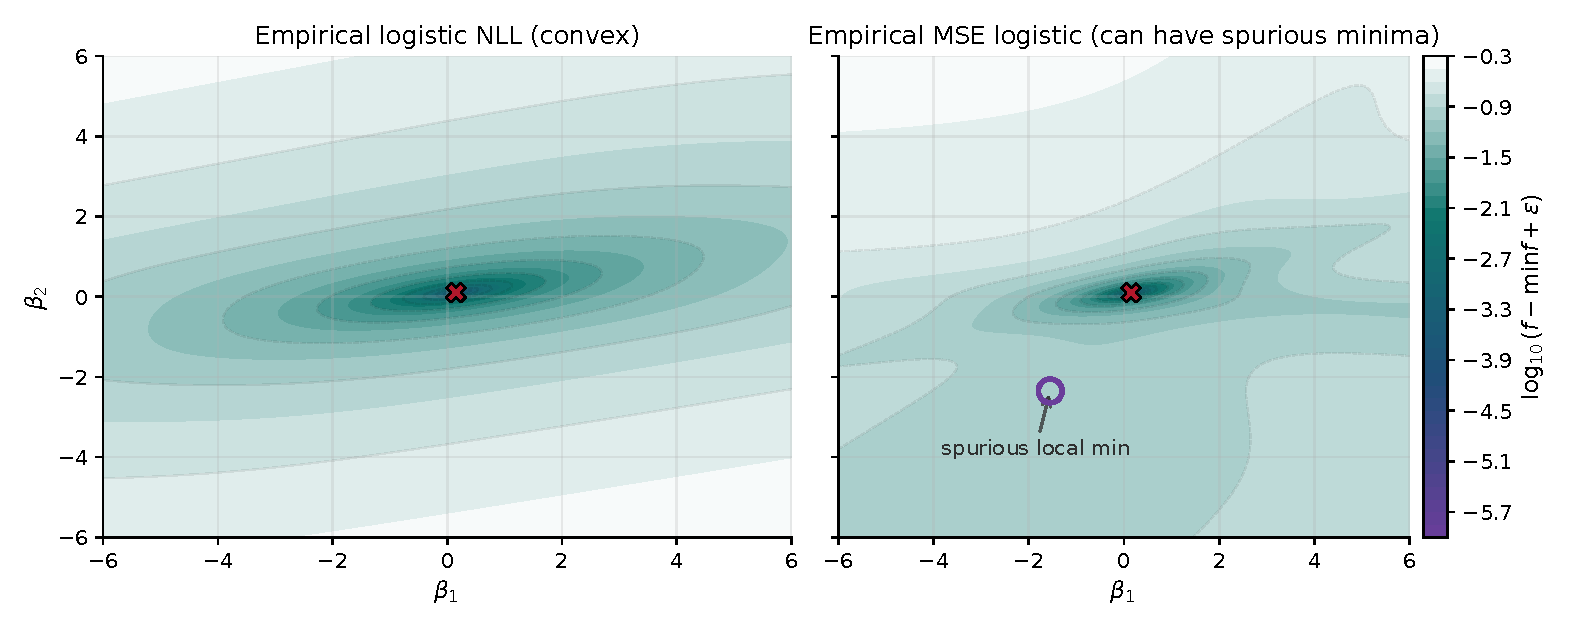
\includegraphics[width=\textwidth]{figures/handouts/convexity_optimization/fig_logistic_empirical_spurious}
  \caption{Empirical logistic landscapes on the dataset in \Cref{ex:logistic-empirical-spurious}.
  The plots show $\log_{10}(f-\min f+\varepsilon)$ for each objective.
  The red X marks the global minimizer in each panel.
  Left: the NLL is convex (one basin).
  Right: the squared-loss objective can have a spurious local minimum (circled), so a local method can get stuck.}
  \label{fig:logistic-empirical-spurious}
\end{figure}

\begin{figure}[t]
  \centering
  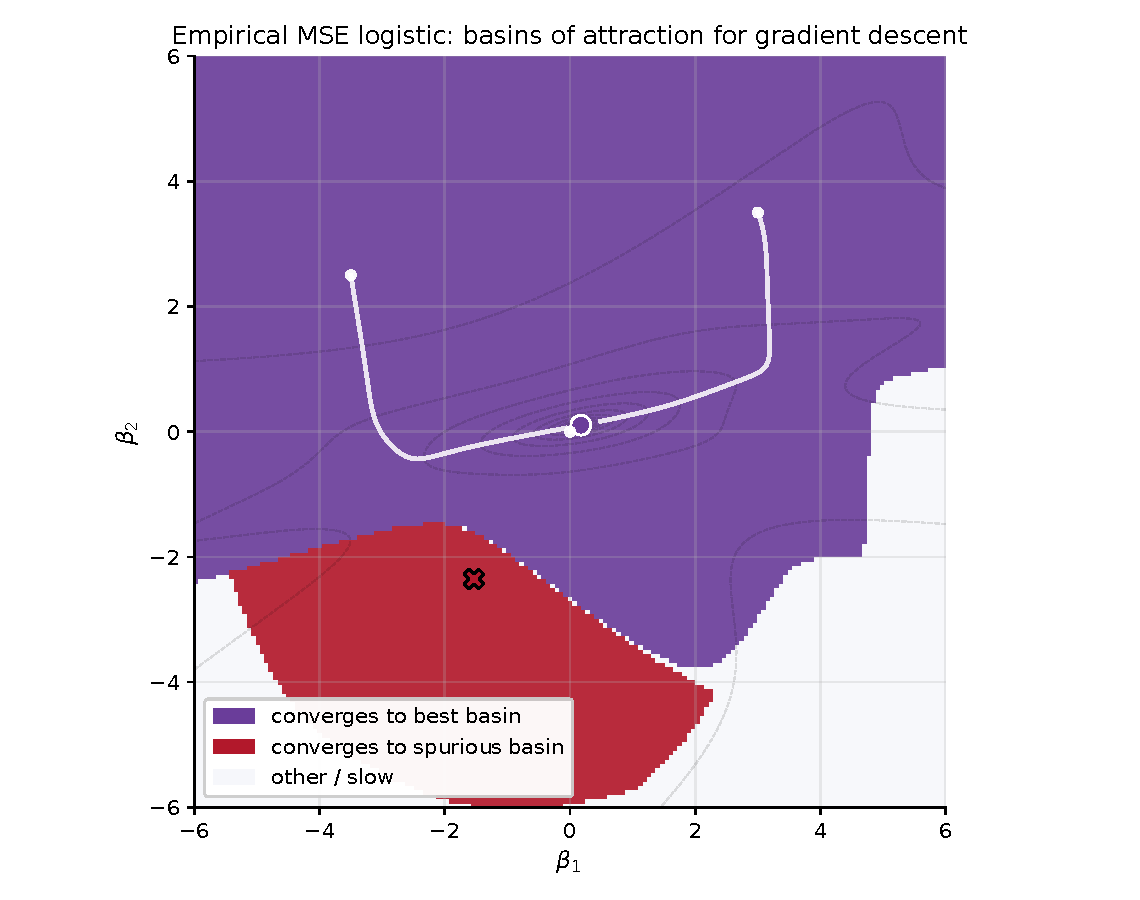
\includegraphics[width=0.92\textwidth]{figures/handouts/convexity_optimization/fig_logistic_empirical_basins}
  \caption{Basins of attraction for gradient descent on the empirical MSE-logistic objective in \Cref{ex:logistic-empirical-spurious}.
  The purple dot and red X mark the two local minimizers.
  Each initialization is colored by which local minimizer fixed-step GD (with $\eta=0.6$) converges to, and the overlaid paths show a few representative trajectories.}
  \label{fig:logistic-empirical-basins}
\end{figure}

Now assume a realizable population model:
\[
Y\mid X=x \sim \mathrm{Bernoulli}(p^\star(x)),
\qquad
p^\star(x) = \sigma(x^\top\beta^\star).
\]
Then the expected squared loss decomposes as
\[
\E\big[(Y-\sigma(X^\top\beta))^2\mid X\big]
= p^\star(X)(1-p^\star(X)) + \big(p^\star(X)-\sigma(X^\top\beta)\big)^2,
\]
so (up to an additive constant) the population objective becomes
\begin{equation}
R(\beta) = \E\big[(\sigma(X^\top\beta)-\sigma(X^\top\beta^\star))^2\big].
\label{eq:logistic-pop-risk}
\end{equation}

\begin{proposition}[One-point monotonicity in the realizable population squared-loss risk]
\label{prop:logistic-pop-one-point}
Assume $\E[\norm{X}_2]<\infty$, and let $R$ be as in \eqref{eq:logistic-pop-risk}. Then for all $\beta$,
\begin{equation}
\ip{\nabla R(\beta)}{\beta-\beta^\star} \ge 0.
\label{eq:one-point}
\end{equation}
In particular, along any ray $\beta(t)=\beta^\star+t(\beta-\beta^\star)$, the function $t\mapsto R(\beta(t))$ is nondecreasing for $t\ge 0$.
\end{proposition}

The next exercise isolates the population monotonicity calculation; structurally it plays the same role as the first-order convexity arguments in the Optimization unit.
\begin{exercise}[One-point monotonicity for realizable MSE-logistic]
\label{ex:logistic-one-point}
Prove \Cref{prop:logistic-pop-one-point}.
Let $\eta=X^\top\beta$ and $\eta^\star=X^\top\beta^\star$.
\begin{enumerate}[leftmargin=*]
  \item Differentiate under the expectation in \eqref{eq:logistic-pop-risk} to show that
  \[
  \nabla R(\beta)
  =2\,\E\Big[(\sigma(\eta)-\sigma(\eta^\star))\,\sigma'(\eta)\,X\Big].
  \]
  \item Show that
  \[
  \ip{\nabla R(\beta)}{\beta-\beta^\star}
  =2\,\E\Big[\sigma'(\eta)\,(\sigma(\eta)-\sigma(\eta^\star))(\eta-\eta^\star)\Big],
  \]
  and conclude it is nonnegative using only that $\sigma$ is increasing and $\sigma'\ge 0$.
  \item Deduce the ray-monotonicity statement by differentiating $g(t)=R(\beta^\star+t(\beta-\beta^\star))$.
\end{enumerate}
\end{exercise}

\SolutionBox[14]{%
\emph{Part (1).}
Differentiate \eqref{eq:logistic-pop-risk} under the expectation:
\[
R(\beta)=\E\big[(\sigma(X^\top\beta)-\sigma(X^\top\beta^\star))^2\big].
\]
Using the chain rule, $\nabla_\beta\sigma(X^\top\beta)=\sigma'(X^\top\beta)\,X$, hence
\[
\nabla R(\beta)
=2\,\E\Big[(\sigma(\eta)-\sigma(\eta^\star))\,\sigma'(\eta)\,X\Big],
\qquad
\eta=X^\top\beta,\ \eta^\star=X^\top\beta^\star.
\]

\emph{Part (2).}
Take the inner product with $(\beta-\beta^\star)$ and use $\ip{X}{\beta-\beta^\star}=\eta-\eta^\star$:
\[
\ip{\nabla R(\beta)}{\beta-\beta^\star}
=2\,\E\Big[\sigma'(\eta)\,(\sigma(\eta)-\sigma(\eta^\star))(\eta-\eta^\star)\Big].
\]
Since $\sigma'(\eta)\ge 0$ and $\sigma$ is increasing, we have
$(\sigma(\eta)-\sigma(\eta^\star))(\eta-\eta^\star)\ge 0$ pointwise.
Therefore the integrand is pointwise nonnegative, and the expectation is nonnegative as claimed.

\emph{Part (3) (ray monotonicity).}
For the ray $\beta(t)=\beta^\star+t(\beta-\beta^\star)$, define $g(t)=R(\beta(t))$.
By the chain rule,
\[
g'(t)=\ip{\nabla R(\beta(t))}{\beta-\beta^\star}\ge 0,
\]
so $t\mapsto R(\beta(t))$ is nondecreasing for $t\ge 0$.
(The argument uses only that the link is increasing with nonnegative derivative, so it holds for any such link function.)%
}

\begin{corollary}[Realizable population MSE-logistic has no spurious local minima]
\label{cor:logistic-pop-no-spurious}
Under the assumptions of \Cref{prop:logistic-pop-one-point}, every local minimizer of the realizable population risk $R$ in \eqref{eq:logistic-pop-risk} is global.
If in addition $\E[XX^\top]\succ 0$, then the unique global minimizer is $\beta^\star$.
\end{corollary}

\begin{exercise}[Stationarity + one-point monotonicity $\Rightarrow$ no spurious local minima]
\label{ex:logistic-one-point-no-spurious}
Prove \Cref{cor:logistic-pop-no-spurious} from \Cref{prop:logistic-pop-one-point}.
\begin{enumerate}[leftmargin=*]
  \item Let $\bar\beta$ be a local minimizer. Since $R$ is differentiable, $\nabla R(\bar\beta)=0$.
  Combine this with \Cref{eq:one-point} to show that
  \[
    0
    = \ip{\nabla R(\bar\beta)}{\bar\beta-\beta^\star}
    = 2\,\E\Big[\sigma'(\bar\eta)\,(\sigma(\bar\eta)-\sigma(\eta^\star))(\bar\eta-\eta^\star)\Big],
  \]
  where $\bar\eta=X^\top\bar\beta$ and $\eta^\star=X^\top\beta^\star$.
  Conclude that $\sigma(X^\top\bar\beta)=\sigma(X^\top\beta^\star)$ almost surely.
  \item Deduce that $R(\bar\beta)=0$, so $\bar\beta$ is a global minimizer.
  \item For uniqueness: show that if $R(\beta)=0$, then $X^\top(\beta-\beta^\star)=0$ almost surely, and deduce $\beta=\beta^\star$ under $\E[XX^\top]\succ 0$.
\end{enumerate}
\end{exercise}

\SolutionBox[14]{%
\emph{Part (1).}
Let $\bar\beta$ be a local minimizer of the differentiable function $R$.
Then $\nabla R(\bar\beta)=0$.
Applying \Cref{prop:logistic-pop-one-point} at $\beta=\bar\beta$ gives
\[
0
= \ip{\nabla R(\bar\beta)}{\bar\beta-\beta^\star}
= 2\,\E\Big[\sigma'(\bar\eta)\,(\sigma(\bar\eta)-\sigma(\eta^\star))(\bar\eta-\eta^\star)\Big],
\qquad \bar\eta=X^\top\bar\beta,\ \eta^\star=X^\top\beta^\star.
\]
The integrand is pointwise nonnegative because $\sigma'(\bar\eta)\ge 0$ and $\sigma$ is increasing, so the expectation can vanish only if the integrand is zero almost surely.
Since $\sigma'(z)>0$ for every finite $z$, this implies
\[
(\sigma(\bar\eta)-\sigma(\eta^\star))(\bar\eta-\eta^\star)=0
\qquad\text{almost surely.}
\]
Because $\sigma$ is strictly increasing, the product above is zero if and only if $\bar\eta=\eta^\star$, equivalently $\sigma(X^\top\bar\beta)=\sigma(X^\top\beta^\star)$ almost surely.

\emph{Part (2).}
If $\sigma(X^\top\bar\beta)=\sigma(X^\top\beta^\star)$ almost surely, then the integrand in \eqref{eq:logistic-pop-risk} vanishes almost surely, so
\[
R(\bar\beta)=\E\big[(\sigma(X^\top\bar\beta)-\sigma(X^\top\beta^\star))^2\big]=0.
\]
Since $R(\beta^\star)=0$ as well, $\bar\beta$ is a global minimizer.

\emph{Part (3) (uniqueness).}
If $R(\beta)=0$, then
\[
\E\big[(\sigma(X^\top\beta)-\sigma(X^\top\beta^\star))^2\big]=0,
\]
so $\sigma(X^\top\beta)=\sigma(X^\top\beta^\star)$ almost surely.
Since $\sigma$ is strictly increasing, this implies $X^\top(\beta-\beta^\star)=0$ almost surely.
Taking expectations yields
$(\beta-\beta^\star)^\top\E[XX^\top](\beta-\beta^\star)=0$.
If $\E[XX^\top]\succ 0$, then the quadratic form is strictly positive unless $\beta=\beta^\star$, so $\beta^\star$ is the unique global minimizer.%
}

The population MSE-logistic risk is nonconvex, but it still has the simple geometry that moving away from $\beta^\star$ does not help along any ray from $\beta^\star$.
This is qualitatively different from objectives like ecological logistic regression (\Cref{sec:ecological-logistic}), where aggregation introduces intrinsic nonconvexity and the landscape can have many distinct basins even under a clean population model.

Even with this benign global geometry, gradient descent can be slow because of saturation and flat plateaus.
The one-point monotonicity in \Cref{prop:logistic-pop-one-point} is a global geometry guarantee, but it is not a rate guarantee.
Far from $\beta^\star$, the squared-loss logistic objective can become very flat because the logistic link saturates:
$\sigma(z)\to 0$ or $1$ and $\sigma'(z)\to 0$ as $|z|\to\infty$.
The squared-loss gradient carries a factor of $\sigma'(X^\top\beta)$, so when the model is very confident (large $|X^\top\beta|$), the gradient can be tiny even if the objective value is not close to its minimum.
This mirrors the ``confidence weights'' story for convex NLL objectives:
in logistic NLL, curvature is largest near the decision boundary, while very confident points contribute little.
For squared loss, that same saturation suppresses the \emph{descent signal} itself, producing plateaus where $\norm{\nabla R(\beta)}_2$ is small even though $R(\beta)-R(\beta^\star)$ is not.

\begin{proposition}[Realizable squared-loss logistic: arbitrarily flat far from $\beta^\star$]
\label{prop:logistic-pop-flat}
Assume $\E[\norm{X}_2]<\infty$ and let $R$ be the realizable population risk \eqref{eq:logistic-pop-risk}.
Define $g(t)=R(t\beta^\star)$ for $t\ge 1$.
Then:
\begin{enumerate}[leftmargin=*]
  \item $g$ is nondecreasing on $[1,\infty)$ and converges to a finite limit $g(\infty)$.
  \item $\lim_{t\to\infty} g'(t)=0$ and $\lim_{t\to\infty}\norm{\nabla R(t\beta^\star)}_2=0$.
  \item If $\Pr(X^\top\beta^\star\neq 0)>0$, then $g(\infty)>0$.
\end{enumerate}
In particular, there are directions along which the landscape becomes arbitrarily flat even though the excess risk stays bounded away from $0$.
\end{proposition}

\emph{Proof idea.} See Exercise~\ref{ex:logistic-plateau}.

\begin{exercise}[Prove the plateau]
\label{ex:logistic-plateau}
In the realizable population model, let $g(t)=R(t\beta^\star)$ for $t\ge 1$.
\begin{enumerate}[leftmargin=*]
  \item Show that
  \[
    g'(t)=2\,\E\big[(\sigma(t\eta^\star)-\sigma(\eta^\star))\,\sigma'(t\eta^\star)\,\eta^\star\big],
    \qquad \eta^\star=X^\top\beta^\star,
  \]
  and conclude that $g$ is nondecreasing (hence $g(t)\to g(\infty)$ since $0\le g(t)\le 1$).
  \item Show that $g'(t)\to 0$ and $\nabla R(t\beta^\star)\to 0$ as $t\to\infty$.
  Interpret this as: \emph{without} a PL/strong-convexity-type condition, small gradient does not imply near-optimality.
  \item Assume $\Pr(\eta^\star\neq 0)>0$.
  Show that $g(\infty)>0$.
\end{enumerate}
\end{exercise}

\SolutionBox[12]{%
Write $\eta^\star=X^\top\beta^\star$ so that $g(t)=\E[(\sigma(t\eta^\star)-\sigma(\eta^\star))^2]$.

\emph{Part (1).}
Differentiate under the expectation:
by the chain rule,
\[
\frac{d}{dt}\sigma(t\eta^\star)=\sigma'(t\eta^\star)\,\eta^\star,
\]
so
\[
g'(t)
=\E\Big[2(\sigma(t\eta^\star)-\sigma(\eta^\star))\cdot \sigma'(t\eta^\star)\,\eta^\star\Big]
=2\,\E\big[(\sigma(t\eta^\star)-\sigma(\eta^\star))\,\sigma'(t\eta^\star)\,\eta^\star\big].
\]
For $t\ge 1$, $\sigma(t\eta^\star)-\sigma(\eta^\star)$ has the same sign as $(t-1)\eta^\star$ since $\sigma$ is increasing.
Because $\sigma'\ge 0$, the integrand is pointwise nonnegative, hence $g'(t)\ge 0$ and $g$ is nondecreasing.
Since $g(t)\in[0,1]$, it follows that $g(t)\to g(\infty)$ for some finite limit $g(\infty)$.

\emph{Part (2).}
For each fixed $\eta^\star\neq 0$, we have $t\eta^\star\to \pm\infty$ and therefore $\sigma'(t\eta^\star)\to 0$ as $t\to\infty$.
Also,
\[
\big|(\sigma(t\eta^\star)-\sigma(\eta^\star))\,\sigma'(t\eta^\star)\,\eta^\star\big|
\le \sigma'(0)\,|\eta^\star|
\le \sigma'(0)\,\norm{\beta^\star}_2\,\norm{X}_2,
\]
which is integrable since $\E[\norm{X}_2]<\infty$.
We will use the following standard fact: if random variables $Z_t$ satisfy $|Z_t|\le W$ with $\E[W]<\infty$ and $Z_t\to 0$ almost surely, then $\E[Z_t]\to 0$.
Applying this fact here gives $g'(t)\to 0$ as $t\to\infty$.

\smallskip
Similarly, differentiating \eqref{eq:logistic-pop-risk} gives
\[
\nabla R(t\beta^\star)
=2\,\E\big[(\sigma(t\eta^\star)-\sigma(\eta^\star))\,\sigma'(t\eta^\star)\,X\big].
\]
The integrand norm is bounded by $2\sigma'(0)\norm{X}_2$, and for each fixed $X$ the factor $\sigma'(t\eta^\star)$ tends to $0$ (or the bracketed term vanishes when $\eta^\star=0$), so the same reasoning lets us pass the limit through the expectation and conclude $\nabla R(t\beta^\star)\to 0$.

\emph{Part (3).}
As $t\to\infty$ we have $\sigma(t\eta^\star)\to 1$ when $\eta^\star>0$, $\sigma(t\eta^\star)\to 0$ when $\eta^\star<0$, and $\sigma(t\eta^\star)=\sigma(\eta^\star)=1/2$ when $\eta^\star=0$.
Since $0\le (\sigma(t\eta^\star)-\sigma(\eta^\star))^2\le 1$, we can apply the same fact (with $W=1$) to pass the limit through the expectation and obtain
\[
g(\infty)=\E\Big[(1-\sigma(\eta^\star))^2\mathbf{1}\{\eta^\star>0\} + \sigma(\eta^\star)^2\mathbf{1}\{\eta^\star<0\}\Big].
\]
If $\Pr(\eta^\star\neq 0)>0$, then the integrand is strictly positive on $\{\eta^\star\neq 0\}$, so $g(\infty)>0$.

Along this ray, the risk can remain bounded away from $0$ while the gradient (and directional derivative) goes to $0$.
Without a condition like PL/strong convexity, a small gradient does not by itself certify near-optimality.
}

Conditions like strong convexity or the PL inequality (\Cref{def:pl-inequality}) prevent this phenomenon: they rule out large flat regions away from the optimum by relating gradient size to suboptimality.
\Cref{prop:logistic-pop-flat} shows the realizable squared-loss logistic risk does not have such a global guarantee in general.

In the realizable population model, the one-point monotonicity in \Cref{prop:logistic-pop-one-point} is a \emph{global} geometric statement.
To get an actual rate for gradient descent, we also need a \emph{local curvature} condition near $\beta^\star$.
One simple sufficient condition is bounded features, which implies local strong convexity (hence a linear rate) around the optimum.

\begin{proposition}[Local linear convergence of gradient descent near $\beta^\star$]
\label{prop:logistic-pop-local-rate}
Assume $\E[XX^\top]\succeq \lambda I_d$ and $\norm{X}_2\le R$ almost surely for some $\lambda,R>0$.
Then at $\beta^\star$,
\[
\Hess R(\beta^\star)\succeq m_0 I_d,
\qquad
m_0 = 2\,\sigma'(R\norm{\beta^\star}_2)^2\,\lambda,
\]
and there exist $r>0$ and constants $0<m\le L<\infty$ such that the population risk $R$ in \eqref{eq:logistic-pop-risk} is $m$-strongly convex and $L$-smooth on the ball $\{\beta:\ \norm{\beta-\beta^\star}_2\le r\}$.
Consequently, gradient descent with step size $1/L$ initialized in this ball satisfies
\[
R(\beta^{(k)})-R(\beta^\star)
\le \left(1-\frac{m}{L}\right)^k\bigl(R(\beta^{(0)})-R(\beta^\star)\bigr)
\qquad\text{(see \citealp[\S9.3]{boyd_vandenberghe_2004_convex}).}
\]
\end{proposition}

\begin{proof}
Differentiate \eqref{eq:logistic-pop-risk} twice.
At $\beta=\beta^\star$, the cross term vanishes and the Hessian simplifies to
\[
\Hess R(\beta^\star)=2\,\E\big[\sigma'(X^\top\beta^\star)^2\,XX^\top\big].
\]
Since $\norm{X^\top\beta^\star}\le \norm{X}_2\norm{\beta^\star}_2\le R\norm{\beta^\star}_2$ almost surely, we have
$\sigma'(X^\top\beta^\star)\ge \sigma'(R\norm{\beta^\star}_2)>0$ almost surely (since $\sigma'$ is even and decreases with $|z|$), hence
\[
\Hess R(\beta^\star)\succeq 2\,\sigma'(R\norm{\beta^\star}_2)^2\,\E[XX^\top]\succeq 2\,\sigma'(R\norm{\beta^\star}_2)^2\,\lambda I_d.
\]
This is the claimed bound with $m_0=2\,\sigma'(R\norm{\beta^\star}_2)^2\,\lambda$.
Because $R$ is twice continuously differentiable and $\norm{X}_2\le R$ almost surely, $\Hess R(\beta)$ varies continuously in $\beta$ and is bounded on compact sets.
Therefore, on a sufficiently small ball around $\beta^\star$, the Hessian is bounded below by (say) $\tfrac12 m_0 I_d$ and above by $L I_d$ for some finite $L$, which gives local strong convexity and smoothness.
The linear convergence rate for gradient descent on an $m$-strongly convex and $L$-smooth function is standard (cited above).
\end{proof}

Under misspecification, hard multimodality can return.
If $p^\star(x)$ is not representable as $\sigma(x^\top\beta)$ (e.g.\ marginalizing over latent classes can yield mixtures of logits), then \eqref{eq:one-point} need not hold, and the population squared-loss risk can become bimodal with spurious local minima.
Benign global geometry often hinges on model and data assumptions.
This is one reason MLE (convex NLL) is often more stable than squared-loss fitting in logistic-type binary regression models.

\begin{example}[Misspecification can create a spurious local minimum for squared-loss logistic regression]
\label{ex:logistic-misspecified-spurious}
Consider a 1D feature $X$ that takes values $\{-2,-1,1,2\}$ with equal probability, and parameterize $\beta=(\beta_0,\beta_1)$ so that $q_\beta(x)=\sigma(\beta_0+\beta_1 x)$.
Let the true conditional probabilities be
\[
p^\star(-2)=0.49,\quad p^\star(-1)=0.87,\quad p^\star(1)=0.92,\quad p^\star(2)=0.36.
\]
This $p^\star$ is not representable as $q_\beta$, since it is not monotone in $x$.

For the population squared-loss risk $R_{\mathrm{MSE}}(\beta)=\E[(q_\beta(X)-p^\star(X))^2]$, a direct evaluation shows two distinct basins:
numerically, evaluating $R_{\mathrm{MSE}}$ on a grid reveals a global minimizer and a spurious local minimizer.
See \Cref{fig:logistic-landscape-2d}.
\end{example}

\begin{figure}[t]
  \centering
  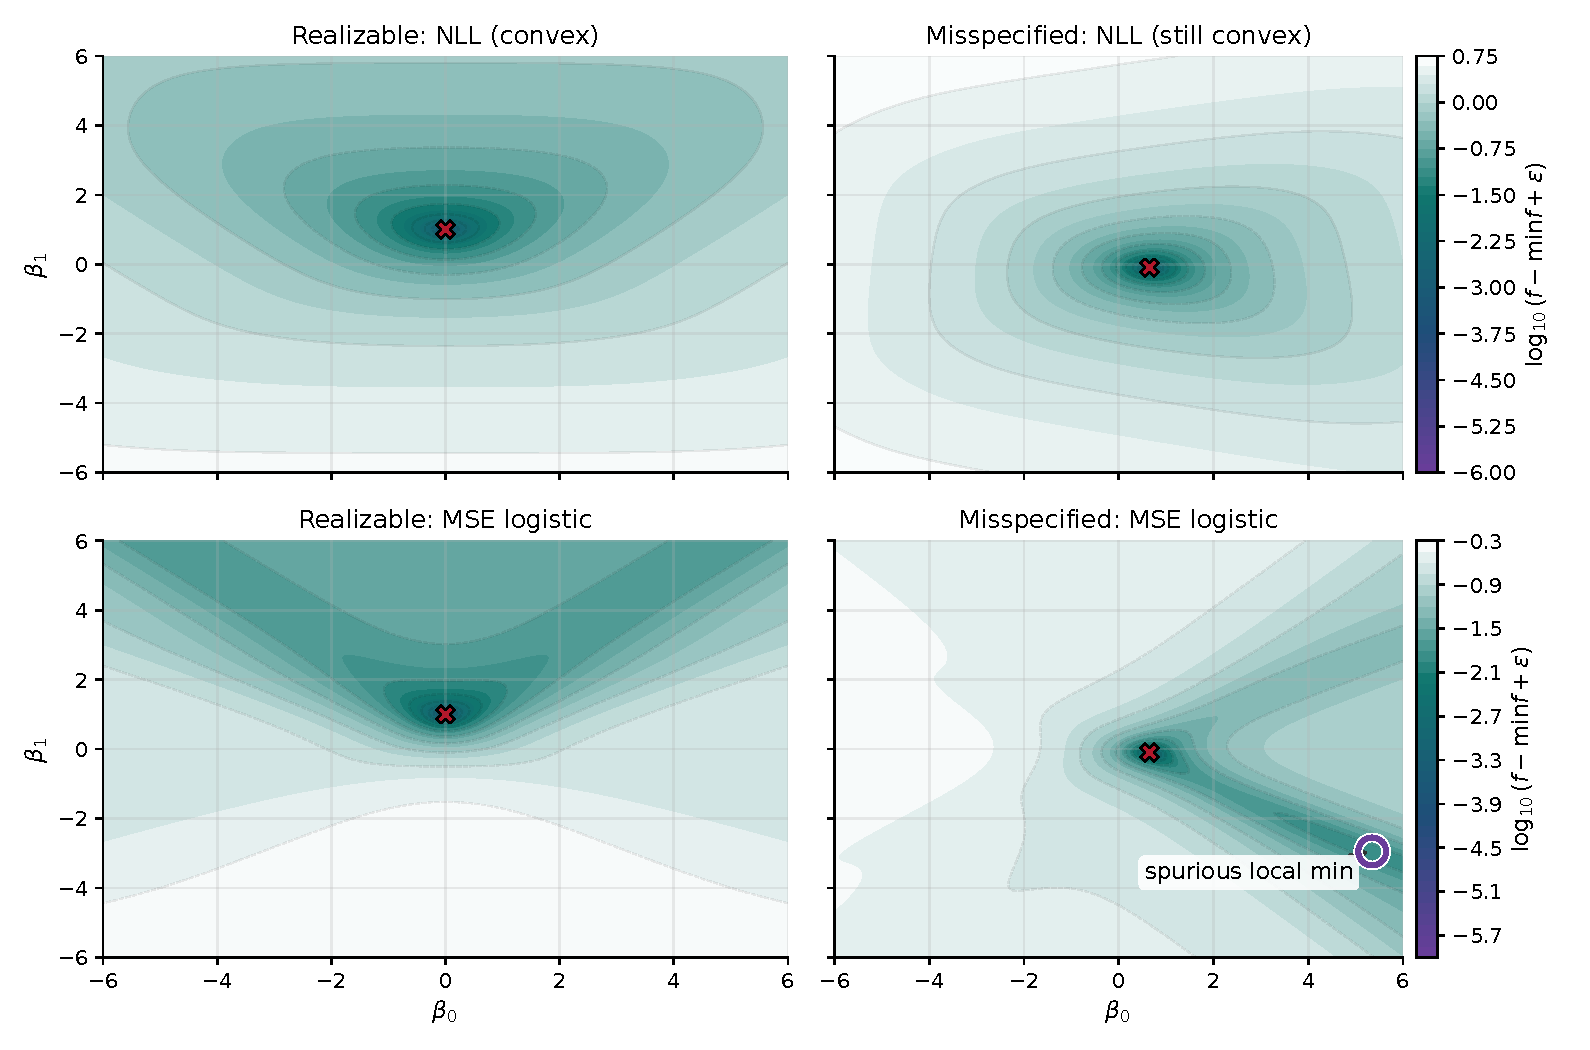
\includegraphics[width=\textwidth]{figures/handouts/convexity_optimization/fig_logistic_landscape_2d}
  \caption{A consistent contourf view of logistic landscapes in a 2D parameterization $\beta=(\beta_0,\beta_1)$.
  The plots show $\log_{10}(f-\min f+\varepsilon)$ for each objective, which makes basins comparable across panels.
  The red X marker indicates the global minimizer in each panel; in the bottom-right plot, the circled point is a spurious local minimum.
  In this example, the NLL landscape is unimodal in both realizable and misspecified settings, while the squared-loss landscape can develop extra basins under misspecification.}
  \label{fig:logistic-landscape-2d}
\end{figure}

% ------------------------------------------------------------
Example~I separates three distinct regimes.
Empirical MSE-logistic can create spurious basins; the realizable population risk has no spurious local minima but can still be slow because of broad plateaus; and misspecification can bring back genuinely wrong stable basins.
The response depends on the regime: use a stable objective when possible, use damping or line search when curvature is unreliable, and use restarts or stronger initializations when multiple basins are present.

% ------------------------------------------------------------
\section[Example II (phase retrieval)]{Example II: multimodality from symmetry, but only global optima in phase retrieval}
\label{sec:phase-retrieval}

In coherent diffraction imaging, optics, and astronomy, sensors measure intensities and lose phase.
A canonical real model is \emph{phase retrieval}:
\[
y_i = (a_i^\top x^\star)^2,\qquad i=1,\dots,m,
\]
where $x^\star\in\R^d$ is the unknown signal and $a_i$ are known sensing vectors.
A standard nonconvex least-squares objective is
\begin{equation}
F(x)=\frac{1}{4m}\sum_{i=1}^m\big((a_i^\top x)^2 - y_i\big)^2.
\label{eq:phase-empirical}
\end{equation}
This objective is nonconvex for structural reasons (it involves squares of linear forms),
and it is \emph{inherently} multimodal because $x^\star$ and $-x^\star$ generate the same data.

Like squared-loss logistic regression, phase retrieval is a smooth, nonconvex least-squares objective.
But here the nonconvexity is driven primarily by a \emph{symmetry}: $x^\star$ and $-x^\star$ generate the same data.
In population (for Gaussian designs), this symmetry produces multiple global optima but \emph{no} suboptimal local minima; the remaining stationary points are saddles.
This is ``benign'' nonconvexity (a strict-saddle picture), and it contrasts with ecological logistic regression (\Cref{sec:ecological-logistic}), where aggregation creates intrinsic nonconvexity and can lead to many distinct basins.
This ``benign geometry'' picture (multiple equivalent global minimizers; strict saddles elsewhere) appears broadly in modern tractable nonconvex problems; see \citet[\S2]{sun_qu_wright_2015_nonconvex_not_scary} and \citet[\S1]{zhang_qu_wright_2020_symmetry_geometry}.

\begin{figure}[t]
  \centering
  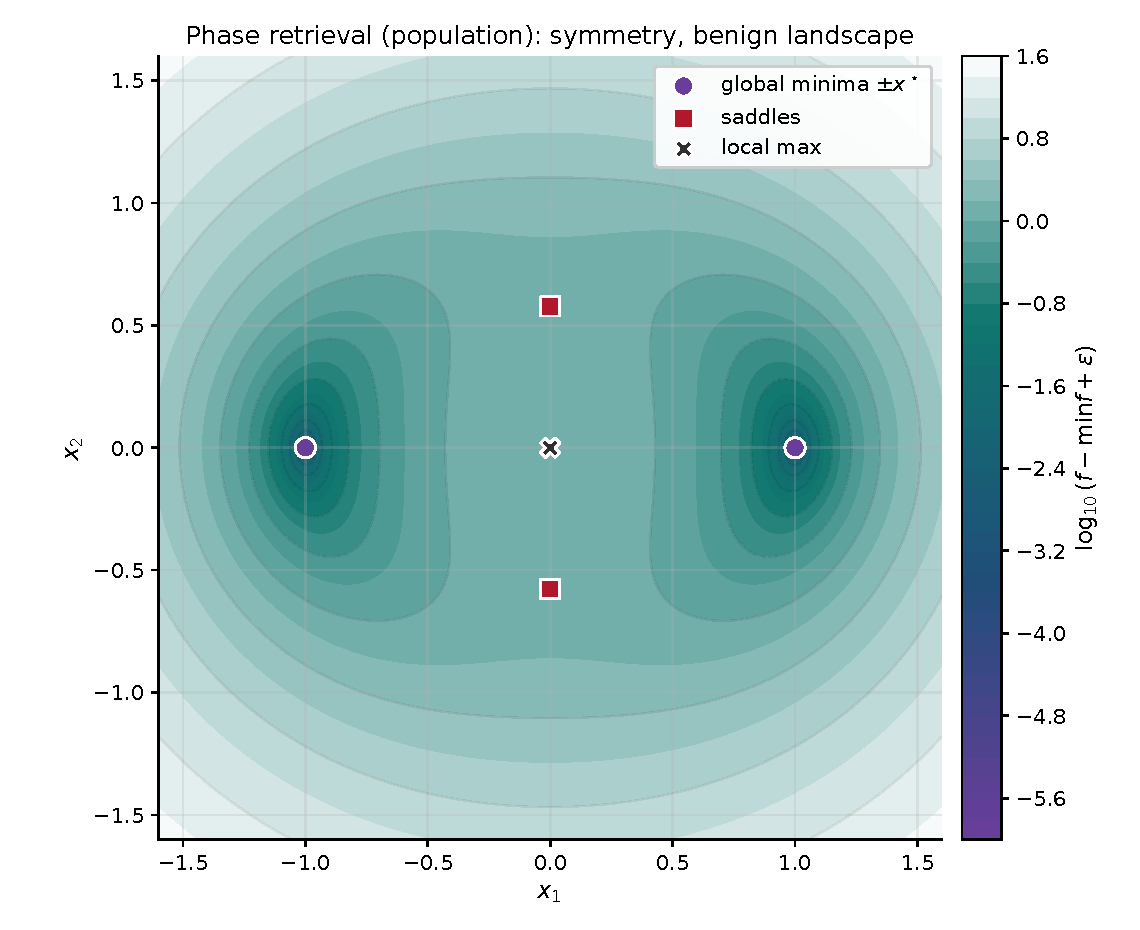
\includegraphics[width=0.86\textwidth]{figures/handouts/convexity_optimization/fig_phase_retrieval_landscape}
  \caption{Population phase retrieval in $d=2$: the landscape is nonconvex and symmetric ($x\sim -x$), but the only local minima are the two global minima $\pm x^\star$; other critical points are saddles or a local maximum at the origin.}
  \label{fig:phase-retrieval-landscape}
\end{figure}

For a clean population model, assume $a\sim N(0,I_d)$ and consider the \emph{population} objective
\begin{equation}
  f(x)=\frac12\,\E\Big[\big((a^\top x)^2 - (a^\top x^\star)^2\big)^2\Big].
  \label{eq:phase-pop}
\end{equation}

\begin{proposition}[Population phase retrieval: nonconvex but no spurious local minima]
\label{prop:phase-retrieval-benign}
For $f$ in \eqref{eq:phase-pop},
\begin{equation}
  f(x)
  =\frac{3}{2}\norm{x}^4 - \norm{x}^2\norm{x^\star}^2 - 2\ip{x}{x^\star}^2 + \frac{3}{2}\norm{x^\star}^4,
  \label{eq:phase-pop-closed-form}
\end{equation}
and the stationary points are:
\begin{enumerate}[leftmargin=*]
  \item global minima $x=\pm x^\star$ (value $0$),
  \item a local maximum at $x=0$,
  \item a saddle set $\{x:\ x\perp x^\star,\ \norm{x}=\norm{x^\star}/\sqrt{3}\}$.
\end{enumerate}
In particular, every local minimum is global.
\end{proposition}

\begin{exercise}[Phase retrieval: derive and classify the population stationary points]
\label{ex:phase-pop-derivation}
Prove \Cref{prop:phase-retrieval-benign}.
\begin{enumerate}[leftmargin=*]
  \item Expand \eqref{eq:phase-pop} and use the Gaussian fourth-moment identities
  \[
  \E[(a^\top u)^4]=3\norm{u}^4,
  \qquad
  \E[(a^\top u)^2(a^\top v)^2]=\norm{u}^2\norm{v}^2 + 2\ip{u}{v}^2,
  \]
  to obtain \eqref{eq:phase-pop-closed-form}.
  \item Differentiate \eqref{eq:phase-pop-closed-form} to get an explicit formula for $\nabla f(x)$.
  \item Solve $\nabla f(x)=0$ by decomposing $x=\alpha x^\star + u$ with $u\perp x^\star$.
  \item Classify the stationary points as global minima, a local maximum, and a saddle set.
\end{enumerate}
\end{exercise}

\SolutionBox[22]{%
\emph{Part (1) (closed form).}
Expanding the square in \eqref{eq:phase-pop} gives
\[
f(x)
=\frac12\,\E\big[(a^\top x)^4\big]
\;-\;\E\big[(a^\top x)^2(a^\top x^\star)^2\big]
\;+\;\frac12\,\E\big[(a^\top x^\star)^4\big].
\]
Apply the stated Gaussian fourth-moment identities with $u=x$ and $v=x^\star$ to get
\[
\E[(a^\top x)^4]=3\norm{x}^4,\qquad
\E[(a^\top x^\star)^4]=3\norm{x^\star}^4,
\]
and
\[
\E[(a^\top x)^2(a^\top x^\star)^2]=\norm{x}^2\norm{x^\star}^2 + 2\ip{x}{x^\star}^2.
\]
Substituting yields \eqref{eq:phase-pop-closed-form}.

\emph{Part (2) (gradient).}
Differentiate \eqref{eq:phase-pop-closed-form}:
\[
\nabla f(x)
= 6\norm{x}^2 x - 2\norm{x^\star}^2 x - 4\ip{x}{x^\star}x^\star
= (6\norm{x}^2-2\norm{x^\star}^2)x - 4\ip{x}{x^\star}x^\star.
\]

\emph{Part (3) (stationary points).}
Let $r=\norm{x^\star}_2$ and decompose $x=\alpha x^\star + u$ with $u\perp x^\star$.
Then $\ip{x}{x^\star}=\alpha r^2$ and $\norm{x}^2=\alpha^2r^2+\norm{u}^2$.
Setting $\nabla f(x)=0$ and matching the $u$ and $x^\star$ components gives
\[
(6\norm{x}^2-2r^2)\,u=0,
\qquad
\alpha\,(6\norm{x}^2-6r^2)=0.
\]
If $u=0$, then either $\alpha=0$ (so $x=0$) or $\norm{x}^2=r^2$ (so $\alpha=\pm 1$ and $x=\pm x^\star$).
If $u\neq 0$, then the first equation forces $\norm{x}^2=r^2/3$, and the second forces $\alpha=0$, hence
$x\perp x^\star$ and $\norm{x}=r/\sqrt{3}$.
This gives exactly the stationary-point list in \Cref{prop:phase-retrieval-benign}.

\emph{Part (4) (classification).}
Since $f$ in \eqref{eq:phase-pop} is an expectation of a square, $f(x)\ge 0$ for all $x$.
Also $f(\pm x^\star)=0$, so $\pm x^\star$ are global minima.

For $x=0$, the expansion \eqref{eq:phase-pop-closed-form} shows
\[
f(0)-f(x)= r^2\norm{x}^2 + 2\ip{x}{x^\star}^2 - \frac{3}{2}\norm{x}^4,
\]
which is strictly positive for all sufficiently small $x\neq 0$ (the quadratic term dominates), so $x=0$ is a local maximum.

Finally, if $x\perp x^\star$ and $\norm{x}=r/\sqrt{3}$, then the univariate restriction $t\mapsto f(x+t x^\star)$ has negative second derivative at $t=0$, so there is a direction of negative curvature.
Hence these points are saddles, and every local minimum is global.%
}

This is symmetry-driven nonconvexity with a strict-saddle geometry:
every non-optimal stationary point has a direction of negative curvature.

Phase retrieval is typically approached via the two-stage template in \Cref{alg:two-stage-template}:
use a cheap global initializer, then run a local method.
In the Gaussian model, there is a clean way to build a provably good direction estimate from a simple moment identity.
Assume the noiseless Gaussian design model $a_i \stackrel{\mathrm{iid}}{\sim} N(0,I_d)$ with measurements $y_i=(a_i^\top x^\star)^2$.
Define the \emph{spectral matrix}
\[
  Y = \frac{1}{m}\sum_{i=1}^m y_i a_i a_i^\top.
\]
Also define the radius estimate
\[
  \hat r^2 = \frac{1}{m}\sum_{i=1}^m y_i,
\]
which satisfies $\E[\hat r^2]=\norm{x^\star}_2^2$.
If $\hat u$ is a unit-norm top eigenvector of $Y$, then the standard spectral initializer is $x^{(0)}=\hat r\,\hat u$.

The next proposition explains why this initialization is reasonable.
It shows that (i) the population matrix $\E[Y]$ has a unique leading eigenvector in the $x^\star$ direction, and (ii) if the empirical $Y$ is close to $\E[Y]$ in operator norm then its leading eigenvector must be close to $\pm x^\star/\norm{x^\star}_2$.
(Here $\norm{M}_{\mathrm{op}}$ denotes the operator norm, i.e.\ the largest absolute eigenvalue for a symmetric matrix $M$.)

\begin{proposition}[Gaussian phase retrieval: why the spectral initializer points at $x^\star$]
\label{prop:phase-spectral-init}
Assume $x^\star\neq 0$, let $a\sim N(0,I_d)$, and set $y=(a^\top x^\star)^2$.
Write $r=\norm{x^\star}_2$ and $u^\star=x^\star/r$.
Define the population matrix
\[
  Y_{\mathrm{pop}} = \E\big[y\,a a^\top\big]
  = \E\big[(a^\top x^\star)^2 a a^\top\big].
\]
Then
\[
  Y_{\mathrm{pop}}=r^2 I_d + 2x^\star(x^\star)^\top,
\]
so the unique leading eigenvector of $Y_{\mathrm{pop}}$ is $u^\star$.
Moreover, if $Y$ is any symmetric matrix satisfying
\[
\norm{Y-Y_{\mathrm{pop}}}_{\mathrm{op}} \le \varepsilon\, r^2
\qquad\text{for some }\varepsilon\in(0,1),
\]
then for every unit-norm leading eigenvector $\hat u$ of $Y$ there exists a sign $s\in\{\pm 1\}$ such that
$\norm{\hat u-su^\star}_2\le \sqrt{2\varepsilon}$.
\end{proposition}

\begin{exercise}[Phase retrieval: why spectral initialization points at $x^\star$]
\label{ex:phase-spectral-spike}
Prove \Cref{prop:phase-spectral-init}.
Conclude that if the empirical matrix $Y$ is close to $Y_{\mathrm{pop}}$ in operator norm, then its top eigenvector is close to $\pm u^\star$ and the spectral initializer $x^{(0)}=\hat r\,\hat u$ is close to $\pm x^\star$.
\emph{Hint:} to compute $Y_{\mathrm{pop}}$, you can either compute entries using the Gaussian fourth-moment identity
$\E[a_i a_j a_k a_\ell]=\delta_{ij}\delta_{k\ell}+\delta_{ik}\delta_{j\ell}+\delta_{i\ell}\delta_{jk}$,
or compute the entries directly by expanding.
For the perturbation bound, compare quadratic forms $v^\top Y v$ and use $|v^\top (Y-Y_{\mathrm{pop}}) v|\le \norm{Y-Y_{\mathrm{pop}}}_{\mathrm{op}}$ for unit $v$.
Finally, explain in a sentence why one expects $\norm{Y-Y_{\mathrm{pop}}}_{\mathrm{op}}$ to be small when $m$ is large in the Gaussian model.
\end{exercise}

\SolutionBox[20]{%
Write $u=x^\star$ and expand $y=(a^\top u)^2=\sum_{k,\ell} u_k u_\ell a_k a_\ell$.
For each entry $(i,j)$,
\[
\E\!\big[y\,a_i a_j\big]
=\sum_{k,\ell} u_k u_\ell\,\E[a_i a_j a_k a_\ell]
=\sum_{k,\ell} u_k u_\ell\bigl(\delta_{ij}\delta_{k\ell}+\delta_{ik}\delta_{j\ell}+\delta_{i\ell}\delta_{jk}\bigr).
\]
The first term gives $\delta_{ij}\sum_k u_k^2=\delta_{ij}\norm{u}_2^2$.
The second and third terms each give $u_i u_j$.
Thus $\E[y\,a_i a_j]=\norm{u}_2^2\,\delta_{ij}+2u_i u_j$, i.e.
$Y_{\mathrm{pop}}=\norm{u}_2^2 I_d + 2uu^\top$.

For eigenvalues, note that $Y_{\mathrm{pop}}u=(\norm{u}_2^2+2\norm{u}_2^2)u=3\norm{u}_2^2 u$.
If $w\perp u$, then $uu^\top w=0$ so $Y_{\mathrm{pop}}w=\norm{u}_2^2 w$.
Hence the unique top eigenspace is $\mathrm{span}\{u\}$.

Let $r=\norm{u}_2$ and $u^\star=u/r$.
Let $\hat u$ be a unit top eigenvector of $Y$.
Write $E=Y-Y_{\mathrm{pop}}$ and assume $\norm{E}_{\mathrm{op}}\le \varepsilon r^2$.
Then
\[
\hat u^\top Y_{\mathrm{pop}} \hat u
= \hat u^\top Y \hat u - \hat u^\top E \hat u
\ge \lambda_{\max}(Y) - \norm{E}_{\mathrm{op}}
\ge (u^\star)^\top Y u^\star - \norm{E}_{\mathrm{op}}
\ge 3r^2 - 2\varepsilon r^2.
\]
On the other hand,
$
\hat u^\top Y_{\mathrm{pop}} \hat u
= r^2 + 2r^2\,|\ip{\hat u}{u^\star}|^2.
$
Combining gives $|\ip{\hat u}{u^\star}|^2\ge 1-\varepsilon$.
Choosing the sign that maximizes the inner product,
\[
\min\{\norm{\hat u-u^\star}_2,\norm{\hat u+u^\star}_2\}^2
=2\bigl(1-|\ip{\hat u}{u^\star}|\bigr)
\le 2\bigl(1-|\ip{\hat u}{u^\star}|^2\bigr)
\le 2\varepsilon.
\]

The matrix $Y$ is an empirical average of i.i.d.\ symmetric matrices with mean $Y_{\mathrm{pop}}$.
To make this quantitative in high dimensions, one uses concentration inequalities for random matrices to bound $\norm{Y-Y_{\mathrm{pop}}}_{\mathrm{op}}$ with high probability; see \citet[\S2.2]{zhang_qu_wright_2020_symmetry_geometry} for discussion and references.
These probability tools are largely orthogonal to our focus here.%
}

Once you have an initialization that is close to $\pm x^\star$, the local stage behaves like the convex story again.
In the Gaussian population objective, $\pm x^\star$ are not only global minima: they are \emph{locally strongly convex} minima, so the standard local strong-convexity analysis from the Optimization unit gives a linear rate while the iterates remain in that neighborhood.

\begin{exercise}[Phase retrieval: local convexity near $\pm x^\star$ in the population objective]
\label{ex:phase-pop-local-strong-convex}
For the population objective $f$ in \eqref{eq:phase-pop-closed-form}, compute the Hessian $\Hess f(x)$ and show that
\[
\Hess f(x^\star)=4\norm{x^\star}_2^2 I_d + 8x^\star(x^\star)^\top.
\]
Deduce the eigenvalues of $\Hess f(x^\star)$ and interpret this as a local condition-number statement near $x^\star$.
\end{exercise}

\SolutionBox[12]{%
Differentiate the gradient formula in the solution to \Cref{ex:phase-pop-derivation}:
for $x\in\R^d$,
\[
\Hess f(x)=12xx^\top + (6\norm{x}_2^2-2\norm{x^\star}_2^2)I_d - 4x^\star(x^\star)^\top.
\]
At $x=x^\star$ this becomes
\[
\Hess f(x^\star)=(12-4)x^\star(x^\star)^\top + 4\norm{x^\star}_2^2 I_d
=8x^\star(x^\star)^\top + 4\norm{x^\star}_2^2 I_d.
\]
Along $u^\star=x^\star/\norm{x^\star}_2$ the eigenvalue is $12\norm{x^\star}_2^2$, and along any direction orthogonal to $x^\star$ the eigenvalue is $4\norm{x^\star}_2^2$.
So near $x^\star$ the population objective is well conditioned (local condition number $3$), which is exactly the regime where local methods behave like in the convex case.%
}

These pieces give the standard Gaussian-model story:
spectral initialization supplies a direction close to $\pm x^\star$, and the local geometry near $\pm x^\star$ is strongly convex, so local methods converge quickly once initialized there.
Rigorous finite-sample analyses follow this template; see \citet[\S2.2]{zhang_qu_wright_2020_symmetry_geometry} and references therein.

Phase retrieval shows a different kind of nonconvexity.
The sign symmetry creates multiple optima, but they are equivalent, and the remaining stationary points are saddles rather than bad local minima.
The right response is therefore not exhaustive global search; it is a coarse initializer, such as a spectral method, followed by local refinement inside the basin of $\pm x^\star$.



% ------------------------------------------------------------
\section[Example III (ecological logistic)]{Example III: hard nonconvexity from aggregation in ecological logistic regression}
\label{sec:ecological-logistic}

In some applications we observe covariates at the unit level but only aggregated outcomes.
For example, we might see covariates $x_{g,1},\dots,x_{g,n_g}$ for individuals in a group (a precinct, a cohort, a batch),
but instead of observing the binary outcomes $Y_{g,i}\in\{0,1\}$ we only observe the group total
\[
Z_g = \sum_{i=1}^{n_g} Y_{g,i}.
\]
Many different binary vectors $(Y_{g,1},\dots,Y_{g,n_g})$ can produce the same total $Z_g$, so the likelihood for $\beta$ must marginalize over a large discrete set of latent ``assignments.''

Assume a logistic model at the unit level:
\[
\Pr(Y_{g,i}=1\mid x_{g,i},\beta)=\sigma(x_{g,i}^\top\beta),
\qquad i=1,\dots,n_g,
\]
with conditional independence across $i$ given the covariates.
Write $p_{g,i}(\beta)=\sigma(x_{g,i}^\top\beta)$.
Then $Z_g$ is a sum of independent but non-identically distributed Bernoulli random variables (a Poisson--binomial model), and the marginal likelihood contains $\binom{n_g}{z_g}$ terms.
The resulting negative log-likelihood is typically nonconvex in $\beta$.
This combinatorial marginalization also creates a separate difficulty that is easy to miss if we focus only on the geometry:
when $n_g$ is large, the likelihood term $\Pr(Z_g=z_g\mid x_{g,1},\dots,x_{g,n_g},\beta)$ can be expensive to evaluate repeatedly inside an optimizer.
The naive computation is literally a sum over $\binom{n_g}{z_g}$ assignments (as in \Cref{ex:eco-logistic-nonconvex}), which is intractable for large groups.
This ``optimization + marginalization'' pattern is common in latent-variable models: hard landscapes and expensive objective evaluations can come together.

An empirical negative log-likelihood objective for $G$ independent groups is
\begin{equation}
  f(\beta)
  =
  -\frac{1}{G}\sum_{g=1}^G \log \Pr(Z_g=z_g \mid x_{g,1},\dots,x_{g,n_g},\beta).
  \label{eq:eco-logistic-obj}
\end{equation}
Two edge cases are instructive.
In the special case where the covariates are constant within each group ($x_{g,i}\equiv x_g$), we have
$Z_g\sim \mathrm{Binomial}(n_g,\sigma(x_g^\top\beta))$, and \eqref{eq:eco-logistic-obj} reduces to the usual convex binomial logistic-regression objective from the Optimization unit.
At the other extreme, if $d=1$ with $\beta=(\beta_0,\beta_1)$ and each group contains covariates in $\pm$ pairs (for every $x$ the value $-x$ appears with the same multiplicity), then the marginal likelihood is symmetric in the slope: it is unchanged under $\beta_1\mapsto -\beta_1$.
This kind of symmetry reflects a genuine non-identifiability from totals alone.

\begin{exercise}[Ecological logistic regression: two easy special cases]
\label{ex:eco-logistic-edge-cases}
\begin{enumerate}[leftmargin=*]
  \item Suppose $x_{g,i}\equiv x_g$ within each group.
  Show that $Z_g\sim \mathrm{Binomial}(n_g,\sigma(x_g^\top\beta))$ and conclude that the corresponding negative log-likelihood is convex in $\beta$.
  \item Assume $d=1$ with $\beta=(\beta_0,\beta_1)$ and suppose the multiset $\{x_1,\dots,x_n\}$ is symmetric: for every $x$ it contains $-x$ with the same multiplicity.
  Show that, for every $z$,
  \[
    \Pr(Z=z\mid x_1,\dots,x_n,(\beta_0,\beta_1))
    =
    \Pr(Z=z\mid x_1,\dots,x_n,(\beta_0,-\beta_1)).
  \]
  Conclude that the likelihood for $\beta_1$ is an even function, so the sign of the slope is not identifiable from $Z$ alone in such a balanced design.
\end{enumerate}
\end{exercise}

\SolutionBox[14]{%
\emph{Part (1).}
If $x_{g,i}\equiv x_g$, then conditional on $x_g$ the unit-level outcomes are i.i.d.\ Bernoulli with success probability $\sigma(x_g^\top\beta)$.
Therefore $Z_g=\sum_{i=1}^{n_g}Y_{g,i}\sim \mathrm{Binomial}(n_g,\sigma(x_g^\top\beta))$.
Up to an additive constant (independent of $\beta$), the per-group negative log-likelihood can be written as a function of the scalar $\eta=x_g^\top\beta$:
\[
\ell_g(\beta)
= -z_g\,\eta + n_g\log(1+e^\eta).
\]
Since $\frac{d^2}{d\eta^2}\ell_g(\eta)=n_g\,\sigma'(\eta)\ge 0$, the map $\eta\mapsto \ell_g(\eta)$ is convex.
Composing a convex function with a linear map $\beta\mapsto x_g^\top\beta$ preserves convexity, so $\ell_g$ is convex in $\beta$.
Summing over $g$ preserves convexity, hence the full objective is convex.

\emph{Part (2).}
Write $p_i(\beta_0,\beta_1)=\sigma(\beta_0+\beta_1 x_i)$.
Replacing $\beta_1$ by $-\beta_1$ replaces $p_i$ by $\tilde p_i=\sigma(\beta_0-\beta_1 x_i)$.
By the assumed symmetry of the multiset $\{x_i\}$, the multiset $\{\tilde p_i\}$ is the same as $\{p_i\}$ up to a permutation (each $x$ is paired with $-x$).
But the distribution of $Z=\sum_i Y_i$ depends only on the multiset of success probabilities, not on how they are ordered, so $\Pr(Z=z\mid x_1,\dots,x_n,(\beta_0,\beta_1))=\Pr(Z=z\mid x_1,\dots,x_n,(\beta_0,-\beta_1))$ for every $z$.
Thus the likelihood is an even function of $\beta_1$, which means the sign of the slope is not identifiable from totals in this balanced design.%
}

This example ties directly to the empirical-versus-population theme from Example~I.
There the bad basins can be a finite-sample artifact under benign population geometry; here the nonconvexity is intrinsic, because even under the correct model and infinite data aggregation forces us to marginalize over discrete latent assignments.
That marginalization step is also the bridge to the Expectation--maximization subsection of the Augmented-state optimization unit: once the assignments are latent, the natural algorithmic object is the EM update map, which alternates exact conditional expectations with parameter updates, rather than a single closed-form convex objective.

To emphasize this, it is useful to look at a \emph{population} version of \eqref{eq:eco-logistic-obj}.
Let $X=(x_1,\dots,x_n)$ denote a random group of covariates and let $Z$ be generated from the model under a true parameter $\beta^\star$.
Define the population objective
\[
F(\beta)=\E\big[-\log \Pr(Z\mid X,\beta)\big].
\]
Because the model is correctly specified, $F$ is minimized at (an observationally equivalent version of) $\beta^\star$.
However, as \Cref{fig:eco-logistic-pop-landscape} illustrates, $F$ can still have multiple separated basins and spurious local minima.

\begin{figure}[H]
  \centering
  \input{figures/handouts/convexity_optimization/fig_ecological_logistic_population_landscape}
  \caption{A toy \emph{population} objective for ecological logistic regression in a 2D parameterization $\beta=(\beta_0,\beta_1)$.
  Each group has $n=6$ units and is equally likely to have covariates $(-4,-3,-2,2,3,4)$, $(-3,-1,1,2,3,4)$, or $(-2,-1,1,2,3,4)$ (in $d=1$); outcomes are generated under $\beta^\star=(0.3,1.2)$.
  The plot shows $\log_{10}(F-\min F+\varepsilon)$, as in \Cref{fig:logistic-landscape-2d}; the red X marks $\beta^\star$ and the open circles mark three spurious local minima in this toy example.}
  \label{fig:eco-logistic-pop-landscape}
\end{figure}

\begin{exercise}[Ecological logistic regression: marginalization and nonconvexity]
\label{ex:eco-logistic-nonconvex}
Fix one group with covariates $x_1,\dots,x_n\in\R^d$ and observe $Z=z$.
Let $p_i(\beta)=\sigma(x_i^\top\beta)$.
\begin{enumerate}[leftmargin=*]
  \item Show that
  \[
    \Pr(Z=z\mid x_1,\dots,x_n,\beta)
    =
    \sum_{\substack{S\subseteq\{1,\dots,n\}\\|S|=z}}
    \ \prod_{i\in S} p_i(\beta)\prod_{j\notin S}\bigl(1-p_j(\beta)\bigr).
  \]
  Interpret this as summing over all ways to choose which $z$ units are the successes.
  \item Specialize to $n=2$ and $z=1$ in $d=1$ with covariates $x_1=a$ and $x_2=b$.
  Let $\ell(\beta)$ be the negative log-likelihood $-\log \Pr(Z=1\mid a,b,\beta)$ with no regularization.
  Show that $\ell''(0)=\tfrac12 ab$.
  Conclude that $\ell$ is not convex whenever $ab<0$.
\end{enumerate}
\end{exercise}

\SolutionBox[20]{%
\emph{Part (1).}
Condition on the covariates.
For any binary vector $y=(y_1,\dots,y_n)\in\{0,1\}^n$, conditional independence gives
\[
\Pr(Y_1=y_1,\dots,Y_n=y_n\mid x_1,\dots,x_n,\beta)
=
\prod_{i=1}^n p_i(\beta)^{y_i}\bigl(1-p_i(\beta)\bigr)^{1-y_i}.
\]
The event $\{Z=z\}$ is the union of all assignments $y$ with exactly $z$ ones, so summing over those assignments yields
\[
\Pr(Z=z\mid x_1,\dots,x_n,\beta)
=
\sum_{\substack{y\in\{0,1\}^n\\ \sum_i y_i=z}}
\ \prod_{i=1}^n p_i(\beta)^{y_i}\bigl(1-p_i(\beta)\bigr)^{1-y_i}.
\]
Reindexing the sum by the subset $S=\{i:\ y_i=1\}$ (which has $|S|=z$) gives the stated formula.

\emph{Part (2).}
For $n=2$ and $z=1$, let $p_1(\beta)=\sigma(a\beta)$ and $p_2(\beta)=\sigma(b\beta)$.
Then
\[
q(\beta)=\Pr(Z=1\mid a,b,\beta)
 = p_1(1-p_2) + (1-p_1)p_2
 = p_1+p_2-2p_1p_2,
\]
and $\ell(\beta)=-\log q(\beta)$.
At $\beta=0$ we have $p_1=p_2=\tfrac12$, so $q(0)=\tfrac12$.
Also $p_1'(\beta)=a\,p_1(1-p_1)$ and $p_2'(\beta)=b\,p_2(1-p_2)$, so $p_1'(0)=a/4$ and $p_2'(0)=b/4$.
A direct differentiation gives $q'(0)=0$ and
\[
q''(0)=-4p_1'(0)p_2'(0)=-4\cdot\frac{a}{4}\cdot\frac{b}{4}=-\frac{ab}{4}.
\]
Since $\ell'=-q'/q$ and $q'(0)=0$, we have $\ell''(0)=-(q''(0)/q(0))$ and therefore
\[
\ell''(0)
=-\frac{q''(0)}{q(0)}
=-\frac{-ab/4}{1/2}
=\frac{ab}{2}.
\]
If $ab<0$, then $\ell''(0)<0$, so $\ell$ is not convex.
}

Even though the landscape can be globally hard (and even the population objective can have spurious basins, as in \Cref{fig:eco-logistic-pop-landscape}), there is still a familiar ``convex'' story \emph{locally} around the true parameter under correct specification.
When the model is locally identifiable, the population objective has a neighborhood of $\beta^\star$ on which it is convex (indeed strongly convex).
One convenient way to see this in ecological logistic regression is to expose the probabilistic structure behind the gradient and Hessian: the observed-data objective involves marginalizing over latent assignments, and its Hessian can be written as a difference of two covariance matrices.
After averaging over the random total $Z$ under the true model, that difference becomes a covariance by the law of total covariance.

\begin{exercise}[Ecological logistic regression: DC structure and local convexity near $\beta^\star$]
\label{ex:eco-logistic-pop-local-convex}
Fix covariates $x_1,\dots,x_n\in\R^d$.
For $\beta\in\R^d$, let $V_1,\dots,V_n$ be independent Bernoulli random variables with
\[
\Pr(V_j=1\mid x_j,\beta)=\sigma(x_j^\top\beta),
\qquad j=1,\dots,n,
\]
and define
\[
U = \sum_{j=1}^n x_j V_j,
\qquad
Z = \sum_{j=1}^n V_j.
\]
For an observed total $Z=z$, write $L_z(\beta)=-\log \Pr(Z=z\mid x_1,\dots,x_n,\beta)$.
\begin{enumerate}[leftmargin=*]
  \item Show the \emph{difference-of-convex (DC)} form
  \[
  L_z(\beta)
  =\sum_{j=1}^n \log\bigl(1+e^{x_j^\top\beta}\bigr)
  -\log\left(\sum_{\substack{S\subseteq\{1,\dots,n\}\\|S|=z}} \exp\Big(\sum_{j\in S} x_j^\top\beta\Big)\right).
  \]
  \item Show that $\nabla L_z(\beta)=\E[U]-\E[U\mid Z=z]$.
  \item Show that $\Hess L_z(\beta)=\mathrm{Cov}(U)-\mathrm{Cov}(U\mid Z=z)$.
  (Hint: for $g(\beta)=\log\sum_k e^{a_k^\top\beta}$, the Hessian is the covariance of the vectors $\{a_k\}$ under the corresponding softmax weights.)
  \item Consider the population objective $F(\beta)=\E[L_Z(\beta)]$ when $Z$ is generated under a true parameter $\beta^\star$.
  Assuming the outer expectation defining $F$ can be differentiated twice under the integral sign, use the conditional law of total covariance,
  \[
    \mathrm{Cov}(U\mid X)=\E[\mathrm{Cov}(U\mid Z,X)\mid X] + \mathrm{Cov}(\E[U\mid Z,X]\mid X),
  \]
  to show that
  \[
    \E\big[\Hess L_Z(\beta^\star)\mid X\big]
    = \mathrm{Cov}\big(\E[U\mid Z,X]\mid X\big)\succeq 0.
  \]
  Deduce that
  \[
    \Hess F(\beta^\star)
    = \E\Big[\mathrm{Cov}\big(\E[U\mid Z,X]\mid X\big)\Big]\succeq 0.
  \]
  Conclude that if $\Hess F(\beta^\star)\succ 0$, then $F$ is locally strongly convex on a neighborhood of $\beta^\star$.
\end{enumerate}
\end{exercise}

\SolutionBox[22]{%
\emph{Part (1).}
Write $\eta_j=x_j^\top\beta$ and $p_j=\sigma(\eta_j)=e^{\eta_j}/(1+e^{\eta_j})$.
For any subset $S$ with $|S|=z$,
\[
\Pr(V_j=1\ \forall j\in S,\ V_j=0\ \forall j\notin S\mid x_1,\dots,x_n,\beta)
=\prod_{j\in S}p_j\prod_{j\notin S}(1-p_j)
=\frac{\exp(\sum_{j\in S}\eta_j)}{\prod_{j=1}^n(1+e^{\eta_j})}.
\]
Summing over all $S$ with $|S|=z$ gives
\[
\Pr(Z=z\mid x_1,\dots,x_n,\beta)
=\frac{\sum_{|S|=z}\exp(\sum_{j\in S}\eta_j)}{\prod_{j=1}^n(1+e^{\eta_j})}.
\]
Taking $-\log$ yields the stated DC representation.

\emph{Parts (2) and (3).}
The first term in $L_z$ has gradient $\sum_j \sigma(\eta_j)x_j$ and Hessian $\sum_j \sigma'(\eta_j)x_jx_j^\top$.
Since $U=\sum_j x_j V_j$ with independent Bernoulli coordinates, these are exactly $\E[U]$ and $\mathrm{Cov}(U)$.

For the second term, define a probability distribution on subsets $S$ of size $z$ by
\[
w_S(\beta)\propto \exp\Big(\sum_{j\in S}x_j^\top\beta\Big),
\qquad |S|=z.
\]
This is the conditional law of the success set $\{j:\ V_j=1\}$ given $Z=z$ under parameter $\beta$.
Therefore
\[
\nabla \log\Big(\sum_{|S|=z} e^{\sum_{j\in S}x_j^\top\beta}\Big)
  = \sum_{|S|=z} w_S(\beta)\sum_{j\in S}x_j
  = \E[U\mid Z=z],
\]
and differentiating once more gives
\[
\Hess\!\left(\log\Big(\sum_{|S|=z} e^{\sum_{j\in S}x_j^\top\beta}\Big)\right)
=\mathrm{Cov}(U\mid Z=z),
\]
which yields $\nabla L_z=\E[U]-\E[U\mid Z=z]$ and $\Hess L_z=\mathrm{Cov}(U)-\mathrm{Cov}(U\mid Z=z)$.

\emph{Part (4).}
Now let $X=(x_1,\dots,x_n)$ be random, and assume we may differentiate the outer expectation in $F(\beta)=\E[L_Z(\beta)]$ twice under the integral sign.
Conditional on $X$ and at $\beta^\star$, take expectations over $Z$:
\[
\E\big[\Hess L_Z(\beta^\star)\mid X\big]
=\mathrm{Cov}(U\mid X)-\E[\mathrm{Cov}(U\mid Z,X)\mid X].
\]
By the conditional law of total covariance,
\[
\mathrm{Cov}(U\mid X)
=\E[\mathrm{Cov}(U\mid Z,X)\mid X] + \mathrm{Cov}(\E[U\mid Z,X]\mid X),
\]
so the difference is
\[
\E\big[\Hess L_Z(\beta^\star)\mid X\big]
=\mathrm{Cov}(\E[U\mid Z,X]\mid X)\succeq 0.
\]
Taking outer expectations gives
\[
\Hess F(\beta^\star)
=\E\big[\Hess L_Z(\beta^\star)\big]
=\E\Big[\mathrm{Cov}(\E[U\mid Z,X]\mid X)\Big]\succeq 0.
\]
If this unconditional Hessian is positive definite, then by continuity of $\Hess F$ there exists a radius $r>0$ such that $\Hess F(\beta)\succeq \tfrac12 \Hess F(\beta^\star)\succ 0$ on $\{\beta:\ \norm{\beta-\beta^\star}_2\le r\}$, which implies local strong convexity of $F$ on that neighborhood.%
}

This example still fits the two-stage template in \Cref{alg:two-stage-template}, but the coarse stage is less structured.
In practice, one often uses multiple random starts or a warm start from a crude convex surrogate, then runs a local optimizer with line search or damping on the true nonconvex objective \eqref{eq:eco-logistic-obj} and keeps the best solution found.

Ecological logistic regression is the genuinely hard case in this note.
Aggregation forces a sum over latent assignments, so the objective can have many distinct basins even under correct specification.
The practical response is usually robust search rather than a single clever local method: several starts, warm starts from crude convex surrogates when available, and then local refinement with damping or line search on the true objective.



% ------------------------------------------------------------
\section{Diagnosing nonconvex objectives}
\label{sec:checklist-streamlined}

``Nonconvex'' is not a single regime.
Squared-loss logistic regression is close to convex: the empirical objective can have spurious minima, yet under realizability the population geometry is benign and locally strongly convex near $\beta^\star$.
Phase retrieval is symmetry-driven: there can be multiple equivalent optima but no bad local minima.
Ecological logistic regression is intrinsically hard because aggregation induces latent assignments and the resulting marginal likelihood can have many distinct basins.
The right response depends on which regime you are in: stable objectives when available, spectral or other coarse initialization when symmetry is the issue, and restarts or stronger surrogates when aggregation drives the hardness.
This is also the lens used in the Expectation--maximization subsection of the Augmented-state optimization unit: the basin picture remains central, but the relevant geometry is now the geometry of the EM operator and its population/sample perturbations.

A useful diagnosis is to ask whether the difficulty comes from finite-sample noise or the population model, from symmetry or non-identifiability, from genuinely suboptimal basins, from the lack of a global guarantee beyond convexity, or simply from poor local conditioning.
Carried back to the main notes, the point is not that nonconvexity is uniformly hopeless.
The real question is which part of the convex story breaks first: the basin structure, the conditioning inside a good basin, or only the finite-sample objective we happen to optimize.

\begin{table}[t]
  \centering
  \small
  \setlength{\tabcolsep}{4pt}
  \begin{tabular}{@{}p{0.18\textwidth}p{0.24\textwidth}p{0.26\textwidth}p{0.24\textwidth}@{}}
    \toprule
    Example & Source of nonconvexity & Global geometry & Typical response \\
    \midrule
    Logistic: NLL vs MSE & objective choice + assumptions & spurious basins can appear empirically/misspecified; realizable population is benign but can be flat & pick a stable objective (NLL), add damping/restarts, check misspecification \\
    Phase retrieval & symmetry ($x\sim -x$) & strict-saddle population landscape; only local minima are global & spectral init + local refinement; perturb/noise to escape saddles \\
    Ecological\newline logistic & aggregation / missing labels & many distinct basins from latent assignments & many restarts; warm starts; keep best \\
    \bottomrule
  \end{tabular}
  \caption{Summary of the three examples by source of nonconvexity, resulting global geometry, and typical response.
  Together the columns instantiate the ``hardness = basins + geometry'' spine developed in the handout.}
  \label{tab:nonconvex-example-summary}
\end{table}

\bibliographystyle{plainnat}
\makeatletter
\begingroup
\let\input@path\@empty
\IfFileExists{references.bib}{%
  \gdef\stat221bibpath{references}%
}{%
  \IfFileExists{../references.bib}{%
    \gdef\stat221bibpath{../references}%
  }{%
    \gdef\stat221bibpath{../../references}%
  }%
}
\endgroup
\makeatother
\bibliography{\stat221bibpath}

\end{document}
"
%   (Low-level direct build: if you invoke latexmk manually, set -jobname to the
%    titled output so the compiled PDF matches the standard naming scheme.)
%     (cd "Lecture Tex/handouts/section 1" && latexmk -pdf -interaction=nonstopmode -halt-on-error \
%       -pdflatex='pdflatex %O "\\def\\STATshowsolutions{1}\\input{%S}"' section_convexity_optimization.tex)
%   (If you prefer the legacy flag name with digits, use a csname:)
%     pdflatex "\expandafter\def\csname STAT221SOLUTIONS\endcsname{1}\documentclass[11pt]{article}

% Make this file compilable from the repo root or within `Lecture Tex/handouts/`.
\makeatletter
\def\input@path{{../../}{../}{Lecture Tex/}}
\makeatother
\input{preamble}
\usepackage{float} % for [H] placement specifier in algorithms

\graphicspath{{../../}{../}{Lecture Tex/}{../../figures/}{../figures/}{Lecture Tex/figures/}}

% ------------------------------------------------------------
% Build toggle for solutions.
% - Student version (default): show workspace boxes, hide solutions.
% - Solutions version: define \STATshowsolutions on the command line.
%   Preferred repo-level build (compiles the titled PDFs directly and clears legacy outputs):
%     python3 scripts/build_handouts.py --section 1
%   Example:
%     pdflatex "\def\STATshowsolutions{1}\input{Lecture Tex/handouts/section 1/section_convexity_optimization.tex}"
%   (Low-level direct build: if you invoke latexmk manually, set -jobname to the
%    titled output so the compiled PDF matches the standard naming scheme.)
%     (cd "Lecture Tex/handouts/section 1" && latexmk -pdf -interaction=nonstopmode -halt-on-error \
%       -pdflatex='pdflatex %O "\\def\\STATshowsolutions{1}\\input{%S}"' section_convexity_optimization.tex)
%   (If you prefer the legacy flag name with digits, use a csname:)
%     pdflatex "\expandafter\def\csname STAT221SOLUTIONS\endcsname{1}\input{Lecture Tex/handouts/section 1/section_convexity_optimization.tex}"
\newif\ifshowsolutions
\showsolutionsfalse
\ifdefined\STATshowsolutions
  \showsolutionstrue
\fi
\ifcsname STAT221SOLUTIONS\endcsname
  \showsolutionstrue
\fi

% Handout-only tcolorbox style for readable title bars.
% The `stat221titlebox` tcolorbox style is defined in `Lecture Tex/preamble.tex`.

% Solution boxes (controlled by \ifshowsolutions).
% Usage: \SolutionBox{<solution body>}
\newcommand{\SolutionBox}[2][10]{%
  \ifshowsolutions
    \begin{tcolorbox}[stat221panelgray,title={Solution}]
    #2
    \end{tcolorbox}
  \else
    \begin{tcolorbox}[stat221panelgray,unbreakable,title={Workspace}]
    \vspace{#1\baselineskip}
    \end{tcolorbox}
  \fi
}

\title{When does nonconvexity make optimization hard?}
\author{}
\date{}

\begin{document}
\maketitle

\section[Nonconvexity and optimization hardness]{When does nonconvexity make optimization hard?}
\label{sec:convexity-opt-hardness-handout}

Optimization in this course starts from minimizing smooth objectives with local information: gradients, Hessians, line searches, and condition numbers describe what a descent method can see near the current iterate.
This handout asks when that local picture ceases to be the whole story once the objective is no longer convex.
The main objects are the landscape itself, the basins created by that landscape, and the local geometry that determines how quickly a method moves within a basin.

That perspective builds directly on the Optimization unit and feeds forward to the Augmented-state optimization unit, where the same basin-versus-geometry split reappears for the EM update map rather than for a single objective.
Logistic regression, phase retrieval, and ecological logistic regression then supply three contrasting regimes: an objective choice that can create misleading empirical basins, a symmetry-driven landscape with multiple equivalent optima but no bad local minima, and an intrinsically hard latent-assignment problem.

% ------------------------------------------------------------
\section[Basins and geometry]{Basins, geometry, and what local methods can promise}
\label{sec:framing-nonconvex}

Nonconvex analysis in Stat~221 still starts from the same local-method toolkit as the convex case:
\emph{smoothness} gives a descent lemma, and \emph{curvature} controls local speed.
What changes is the global question of whether the landscape contains suboptimal basins that can trap a local method away from the best achievable value.

\begin{definition}[Basic vocabulary]
\label{def:basic-vocab-nonconvex}
Let $f:\R^d\to\R$ be differentiable and write $f^\star=\inf_x f(x)$.
\begin{enumerate}[leftmargin=*]
  \item A point $x$ is a \textbf{stationary point} if $\nabla f(x)=0$.
  \item A point $x$ is a \textbf{local minimizer} if $f(x)\le f(x')$ for all $x'$ in some neighborhood of $x$.
  A local minimizer is \textbf{spurious} if $f(x)>f^\star$.
  \item A \textbf{(strict) saddle} is a stationary point $x$ with a direction of negative curvature, i.e.\ there exists $v$ such that $v^\top \Hess f(x)\,v<0$.
  \item Fix an algorithm (e.g.\ gradient descent with a specified step-size rule).
  The \textbf{basin of attraction} of a limit point $\bar x$ is the set of initializations $x^{(0)}$ for which the iterates converge to $\bar x$.
  Basins depend on the method and its hyperparameters.
\end{enumerate}
\end{definition}

In practice, local methods succeed when descent is reliable, stationary points are safe, and the initialization lands in a basin where the local geometry is favorable.
Because this is a statistical optimization class, we will repeatedly separate what comes from finite-sample randomness from what is intrinsic to the underlying model.
Concretely, we distinguish an \emph{empirical} objective (a finite-sample average) from its \emph{population} counterpart (an expectation under a model).
Spurious basins can be finite-sample artifacts, or they can persist in the population depending on the data/model assumptions.

A useful statistical trick, when an empirical landscape is messy, is to study the population objective first.
In convex optimization this is often geometry-preserving, because convexity is closed under addition: empirical averages and expectations cannot create spurious basins.
In nonconvex problems, however, the empirical and population landscapes can differ in either direction:
summing per-sample losses that are individually benign can create multiple basins, while averaging can smooth a pathological finite-sample landscape into a benign population geometry.
Making this comparison quantitative in high dimensions typically requires concentration tools (uniform convergence, operator-norm bounds), which is largely orthogonal to our focus here.

When multiple basins exist, the standard strategy is to combine a cheap coarse initializer with a local refinement stage.
The initializer is problem-specific; the local step uses the same gradient-based toolkit as in the convex setting.
\begin{algorithm}[H]
  \caption{Two-stage template: coarse initialization + local refinement}
  \label{alg:two-stage-template}
  \begin{algorithmic}[1]
    \Require Objective $f$ and its parameterization, plus whatever structure enables a cheap initializer.
    \Ensure A refined estimate $\hat\theta$ for a (near-)minimizer of $f$.
    \State \textbf{Coarse stage:} produce a small set of candidate initializations $\Theta_0$ (e.g.\ spectral/moment methods, a grid search, or a convex relaxation).
    \State Pick $\theta^{(0)}\in\Theta_0$ with the best objective value (or best surrogate score).
    \State \textbf{Local stage:} run a local optimizer (e.g.\ GD + line search, Gauss--Newton, damped Newton) starting from $\theta^{(0)}$ to obtain $\hat\theta$.
    \State Optionally repeat with multiple $\theta^{(0)}$ and keep the best solution.
  \end{algorithmic}
\end{algorithm}

% ------------------------------------------------------------
\section[Optimization hierarchy]{What properties make local methods reliable?}
\label{sec:optimization-hierarchy}

In this course we often analyze local methods (gradient descent, Newton, SGD) under assumptions like ``convex'' or ``strongly convex''; see \citep[\S9.2--9.3]{boyd_vandenberghe_2004_convex}.
Beyond convexity, there are two questions worth separating: can a local method get trapped at a suboptimal stationary point, and if it does converge, is it fast or slow because of conditioning or flat directions?

One useful ``in-between'' global condition is the Polyak--\L{}ojasiewicz (PL) inequality.
\begin{definition}[Polyak--\L{}ojasiewicz (PL) inequality]
\label{def:pl-inequality}
Let $f:\R^d\to\R$ be differentiable and let $f^\star=\inf_x f(x)$.
We say $f$ satisfies the PL inequality with parameter $\mu>0$ if for all $x\in\R^d$,
\[
\frac{1}{2}\norm{\nabla f(x)}_2^2 \ge \mu\bigl(f(x)-f^\star\bigr).
\]
\end{definition}

Every differentiable $m$-strongly convex function satisfies the PL inequality with parameter $\mu=m$, but PL can also hold even when $f$ is not convex.

\begin{proposition}[PL implies no spurious stationary points]
\label{prop:pl-no-spurious-stationary}
If $f$ satisfies the PL inequality (\Cref{def:pl-inequality}) and $\nabla f(x)=0$, then $x$ is a global minimizer of $f$.
\end{proposition}

\begin{proof}
If $\nabla f(x)=0$, then \Cref{def:pl-inequality} gives $0\ge \mu(f(x)-f^\star)$, hence $f(x)\le f^\star$.
By definition $f^\star\le f(x)$, so $f(x)=f^\star$.
\end{proof}

\begin{theorem}[Gradient descent under PL has a linear rate in function value]
\label{thm:gd-pl-linear}
Assume $f$ is $L$-smooth and satisfies the PL inequality with parameter $\mu$.
Then gradient descent with step size $1/L$ satisfies
\[
f(x^{(k)})-f^\star \le \left(1-\frac{\mu}{L}\right)^k \bigl(f(x^{(0)})-f^\star\bigr).
\]
\end{theorem}

This proof uses the same descent-lemma template developed for gradient descent in the Optimization unit.
\begin{exercise}[Gradient descent under PL]
\label{ex:gd-pl-linear}
Prove \Cref{thm:gd-pl-linear}.
\emph{Hint:} use the descent lemma for $L$-smooth functions,
\[
f\!\left(x-\frac{1}{L}\nabla f(x)\right)
\le f(x)-\frac{1}{2L}\norm{\nabla f(x)}_2^2,
\]
then apply the PL inequality (\Cref{def:pl-inequality}) and iterate.
\end{exercise}

\SolutionBox[10]{%
This is the same descent-lemma-plus-PL argument used in the Optimization unit.
By $L$-smoothness, the descent lemma gives
\[
f\!\left(x-\frac{1}{L}\nabla f(x)\right)
\le f(x)-\frac{1}{2L}\norm{\nabla f(x)}_2^2.
\]
Combine with PL to get
\[
f(x^+)-f^\star
\le f(x)-f^\star - \frac{\mu}{L}\bigl(f(x)-f^\star\bigr)
=\left(1-\frac{\mu}{L}\right)\bigl(f(x)-f^\star\bigr),
\]
and iterate.%
}

Even when convergence is guaranteed (e.g.\ under PL), conditioning still matters. The convergence rate depends on the ratio $L/\mu$, which plays the role of a condition number in \Cref{thm:gd-pl-linear}.

We now turn to three examples, each of which keeps the local-method viewpoint from the Optimization unit but changes the global landscape in a different way.
Example I (logistic regression) shows that ``nonconvex'' can still have a benign population geometry (no spurious local minima) while the empirical objective can have spurious basins and the landscape can be flat.
Example II (phase retrieval) is a clean strict-saddle example where multimodality comes from symmetry and the only local minima are global.
Example III (ecological logistic regression) is a likelihood problem with \emph{intrinsic} nonconvexity created by aggregation/partial observation: many different latent ``assignments'' can explain the same group total, so local methods can be highly initialization-dependent.

% ------------------------------------------------------------
\section[Example I (logistic)]{Example I: objective choice and data assumptions in logistic regression}
\label{sec:logistic-bridge}

In binary regression, logistic regression models
\[
\Pr(y_i=1\mid x_i,\beta)=\sigma(x_i^\top\beta),
\]
where $\sigma(z)=\frac{1}{1+e^{-z}}$ is the logistic sigmoid.
The Optimization unit introduces logistic regression through its convex negative log-likelihood and then studies the resulting gradient and Hessian formulas.
Here we keep the regression-coefficient notation $\beta$ used again in the later ecological-logistic example, and we write the convex objective as $L$ so the formulas line up with that development as closely as possible.
For comparison, we will place next to it a squared-loss objective on the predicted probabilities.
\[
L(\beta)
=
\frac{1}{n}\sum_{i=1}^n \Bigl[\log\bigl(1+e^{x_i^\top\beta}\bigr) - y_i x_i^\top \beta\Bigr]
\]
is the convex negative log-likelihood, while
\[
R_{\mathrm{sq}}(\beta)
= \frac{1}{n}\sum_{i=1}^n \bigl(y_i-\sigma(x_i^\top\beta)\bigr)^2
\]
is the squared-loss alternative.
Equivalently, one can write the pair of objectives as
\begin{enumerate}[leftmargin=*]
  \item the convex negative log-likelihood from maximum likelihood, matching the logistic-regression model developed in the Optimization unit:
  \begin{equation}
    \begin{aligned}
      L(\beta)
      &=
      -\frac{1}{n}\sum_{i=1}^n \Bigl[y_i\log \sigma(x_i^\top\beta) + (1-y_i)\log \sigma(-x_i^\top\beta)\Bigr] \\
      &=
      \frac{1}{n}\sum_{i=1}^n \Bigl[\log\bigl(1+e^{x_i^\top\beta}\bigr) - y_i x_i^\top \beta\Bigr].
    \end{aligned}
    \label{eq:logistic-nll}
  \end{equation}
  \item the squared loss on predicted probabilities, also called Brier or calibration loss, which is smooth but generally nonconvex:
  \begin{equation}
    R_{\mathrm{sq}}(\beta)
    = \frac{1}{n}\sum_{i=1}^n \bigl(y_i-\sigma(x_i^\top\beta)\bigr)^2.
    \label{eq:logistic-mse}
\end{equation}
\end{enumerate}

The three logistic regimes that matter here are finite-sample spurious minima, a realizable population landscape with no spurious local minima but broad plateaus, and misspecification, where wrong basins can return even at the population level.

For the convex logistic model from the Optimization unit, the objective $L$ in \eqref{eq:logistic-nll} has a weighted-Gram Hessian and is convex.
In particular, if $X\in\R^{n\times d}$ has rows $x_i^\top$ and $p_i(\beta)=\sigma(x_i^\top\beta)$, then
\begin{equation}
  \Hess L(\beta)
  =\frac{1}{n}X^\top W(\beta)\,X,
  \qquad
  W(\beta)=\mathrm{diag}\bigl(p_i(\beta)(1-p_i(\beta))\bigr)\succeq 0,
  \label{eq:logistic-nll-hess}
\end{equation}
so $L$ is convex.
This is the same Hessian identity proved in the Optimization unit's logistic-regression development, so we will reuse that derivation here and focus on what changes under squared loss.

By contrast, $R_{\mathrm{sq}}$ is smooth but generally nonconvex, and it can have \emph{spurious} local minima at the empirical (finite-sample) level.

To see where the nonconvexity comes from, write $z_i=x_i^\top\beta$ and recall
$\sigma'(z)=\sigma(z)(1-\sigma(z))$ and $\sigma''(z)=\sigma'(z)(1-2\sigma(z))$.
For the empirical squared loss,
\[
\nabla R_{\mathrm{sq}}(\beta)
=\frac{2}{n}\sum_{i=1}^n \bigl(\sigma(z_i)-y_i\bigr)\,\sigma'(z_i)\,x_i,
\]
and differentiating again gives
\[
\Hess R_{\mathrm{sq}}(\beta)
=\frac{2}{n}\sum_{i=1}^n\Big(\sigma'(z_i)^2 + \bigl(\sigma(z_i)-y_i\bigr)\sigma''(z_i)\Big)x_ix_i^\top.
\]
The key observation is that $\sigma''(z)$ changes sign, so the scalar coefficient in parentheses can be negative.
Thus $\Hess R_{\mathrm{sq}}(\beta)$ can be indefinite, and the objective can be nonconvex even though it is smooth.

\begin{example}[Empirical squared-loss logistic regression can have a spurious local minimum]
\label{ex:logistic-empirical-spurious}
Consider $q_\beta(x)=\sigma(x^\top\beta)$ with $\beta\in\R^2$, and the dataset
\[
((x_i,y_i))_{i=1}^8
=\Bigl(
\begin{aligned}[t]
&((-0.54,1.57),0),\ ((0.15,2.62),1),\ ((-0.89,0.66),0),\\
&((-0.22,0.64),0),\ ((-0.01,-0.64),1),\ ((-0.99,3.48),1),\\
&((-0.09,-2.29),1),\ ((-0.74,0.77),1)
\end{aligned}
\Bigr).
\]
The logistic NLL $L$ is convex by \Cref{eq:logistic-nll-hess}, but the squared-loss objective $R_{\mathrm{sq}}$ in \eqref{eq:logistic-mse} has multiple basins, including a suboptimal local minimizer.
See \Cref{fig:logistic-empirical-spurious,fig:logistic-empirical-basins}.
\end{example}

\begin{figure}[t]
  \centering
  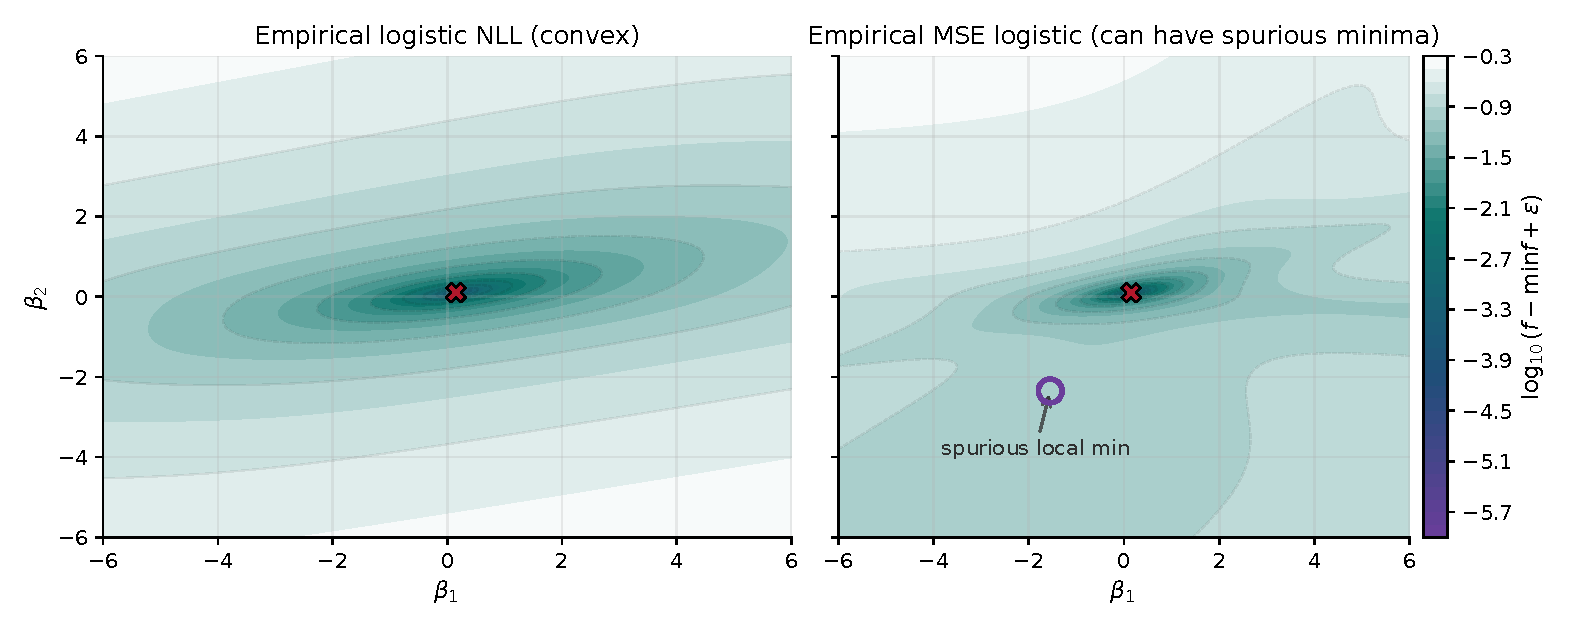
\includegraphics[width=\textwidth]{figures/handouts/convexity_optimization/fig_logistic_empirical_spurious}
  \caption{Empirical logistic landscapes on the dataset in \Cref{ex:logistic-empirical-spurious}.
  The plots show $\log_{10}(f-\min f+\varepsilon)$ for each objective.
  The red X marks the global minimizer in each panel.
  Left: the NLL is convex (one basin).
  Right: the squared-loss objective can have a spurious local minimum (circled), so a local method can get stuck.}
  \label{fig:logistic-empirical-spurious}
\end{figure}

\begin{figure}[t]
  \centering
  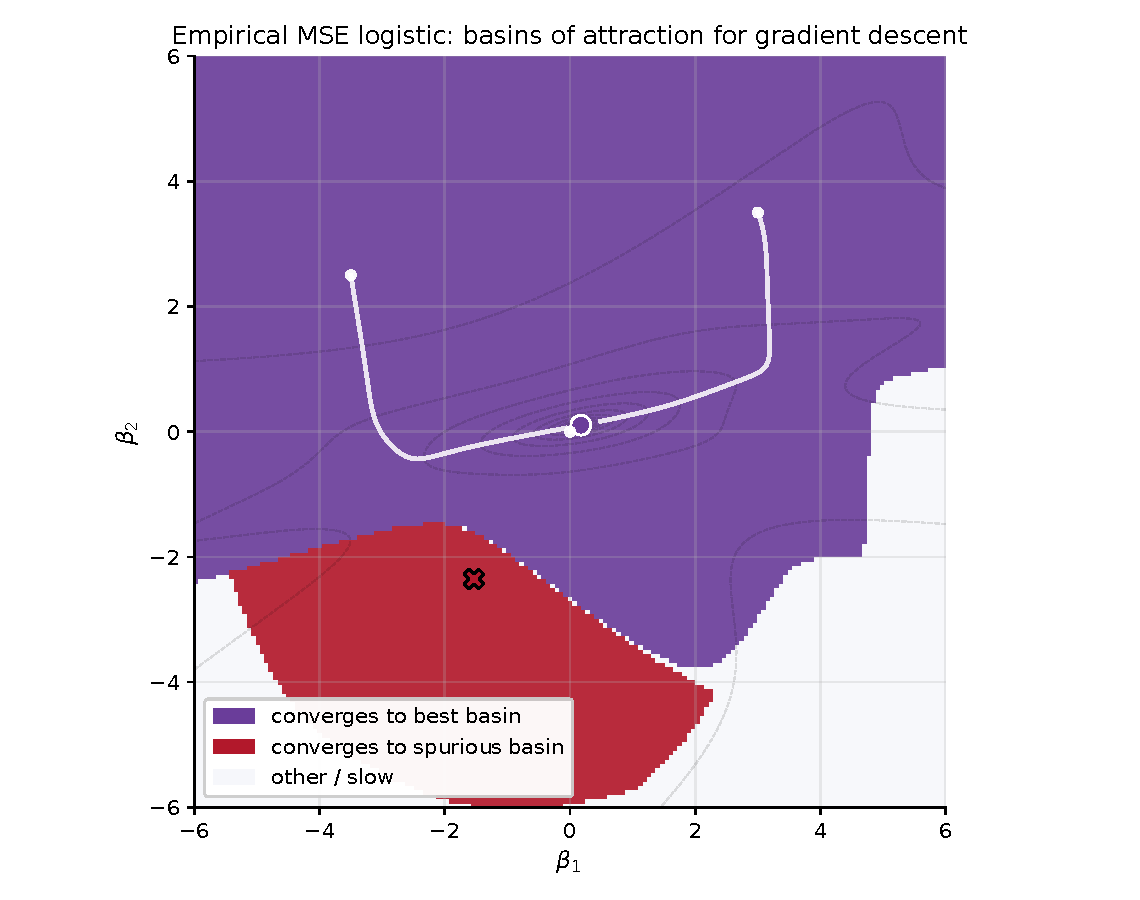
\includegraphics[width=0.92\textwidth]{figures/handouts/convexity_optimization/fig_logistic_empirical_basins}
  \caption{Basins of attraction for gradient descent on the empirical MSE-logistic objective in \Cref{ex:logistic-empirical-spurious}.
  The purple dot and red X mark the two local minimizers.
  Each initialization is colored by which local minimizer fixed-step GD (with $\eta=0.6$) converges to, and the overlaid paths show a few representative trajectories.}
  \label{fig:logistic-empirical-basins}
\end{figure}

Now assume a realizable population model:
\[
Y\mid X=x \sim \mathrm{Bernoulli}(p^\star(x)),
\qquad
p^\star(x) = \sigma(x^\top\beta^\star).
\]
Then the expected squared loss decomposes as
\[
\E\big[(Y-\sigma(X^\top\beta))^2\mid X\big]
= p^\star(X)(1-p^\star(X)) + \big(p^\star(X)-\sigma(X^\top\beta)\big)^2,
\]
so (up to an additive constant) the population objective becomes
\begin{equation}
R(\beta) = \E\big[(\sigma(X^\top\beta)-\sigma(X^\top\beta^\star))^2\big].
\label{eq:logistic-pop-risk}
\end{equation}

\begin{proposition}[One-point monotonicity in the realizable population squared-loss risk]
\label{prop:logistic-pop-one-point}
Assume $\E[\norm{X}_2]<\infty$, and let $R$ be as in \eqref{eq:logistic-pop-risk}. Then for all $\beta$,
\begin{equation}
\ip{\nabla R(\beta)}{\beta-\beta^\star} \ge 0.
\label{eq:one-point}
\end{equation}
In particular, along any ray $\beta(t)=\beta^\star+t(\beta-\beta^\star)$, the function $t\mapsto R(\beta(t))$ is nondecreasing for $t\ge 0$.
\end{proposition}

The next exercise isolates the population monotonicity calculation; structurally it plays the same role as the first-order convexity arguments in the Optimization unit.
\begin{exercise}[One-point monotonicity for realizable MSE-logistic]
\label{ex:logistic-one-point}
Prove \Cref{prop:logistic-pop-one-point}.
Let $\eta=X^\top\beta$ and $\eta^\star=X^\top\beta^\star$.
\begin{enumerate}[leftmargin=*]
  \item Differentiate under the expectation in \eqref{eq:logistic-pop-risk} to show that
  \[
  \nabla R(\beta)
  =2\,\E\Big[(\sigma(\eta)-\sigma(\eta^\star))\,\sigma'(\eta)\,X\Big].
  \]
  \item Show that
  \[
  \ip{\nabla R(\beta)}{\beta-\beta^\star}
  =2\,\E\Big[\sigma'(\eta)\,(\sigma(\eta)-\sigma(\eta^\star))(\eta-\eta^\star)\Big],
  \]
  and conclude it is nonnegative using only that $\sigma$ is increasing and $\sigma'\ge 0$.
  \item Deduce the ray-monotonicity statement by differentiating $g(t)=R(\beta^\star+t(\beta-\beta^\star))$.
\end{enumerate}
\end{exercise}

\SolutionBox[14]{%
\emph{Part (1).}
Differentiate \eqref{eq:logistic-pop-risk} under the expectation:
\[
R(\beta)=\E\big[(\sigma(X^\top\beta)-\sigma(X^\top\beta^\star))^2\big].
\]
Using the chain rule, $\nabla_\beta\sigma(X^\top\beta)=\sigma'(X^\top\beta)\,X$, hence
\[
\nabla R(\beta)
=2\,\E\Big[(\sigma(\eta)-\sigma(\eta^\star))\,\sigma'(\eta)\,X\Big],
\qquad
\eta=X^\top\beta,\ \eta^\star=X^\top\beta^\star.
\]

\emph{Part (2).}
Take the inner product with $(\beta-\beta^\star)$ and use $\ip{X}{\beta-\beta^\star}=\eta-\eta^\star$:
\[
\ip{\nabla R(\beta)}{\beta-\beta^\star}
=2\,\E\Big[\sigma'(\eta)\,(\sigma(\eta)-\sigma(\eta^\star))(\eta-\eta^\star)\Big].
\]
Since $\sigma'(\eta)\ge 0$ and $\sigma$ is increasing, we have
$(\sigma(\eta)-\sigma(\eta^\star))(\eta-\eta^\star)\ge 0$ pointwise.
Therefore the integrand is pointwise nonnegative, and the expectation is nonnegative as claimed.

\emph{Part (3) (ray monotonicity).}
For the ray $\beta(t)=\beta^\star+t(\beta-\beta^\star)$, define $g(t)=R(\beta(t))$.
By the chain rule,
\[
g'(t)=\ip{\nabla R(\beta(t))}{\beta-\beta^\star}\ge 0,
\]
so $t\mapsto R(\beta(t))$ is nondecreasing for $t\ge 0$.
(The argument uses only that the link is increasing with nonnegative derivative, so it holds for any such link function.)%
}

\begin{corollary}[Realizable population MSE-logistic has no spurious local minima]
\label{cor:logistic-pop-no-spurious}
Under the assumptions of \Cref{prop:logistic-pop-one-point}, every local minimizer of the realizable population risk $R$ in \eqref{eq:logistic-pop-risk} is global.
If in addition $\E[XX^\top]\succ 0$, then the unique global minimizer is $\beta^\star$.
\end{corollary}

\begin{exercise}[Stationarity + one-point monotonicity $\Rightarrow$ no spurious local minima]
\label{ex:logistic-one-point-no-spurious}
Prove \Cref{cor:logistic-pop-no-spurious} from \Cref{prop:logistic-pop-one-point}.
\begin{enumerate}[leftmargin=*]
  \item Let $\bar\beta$ be a local minimizer. Since $R$ is differentiable, $\nabla R(\bar\beta)=0$.
  Combine this with \Cref{eq:one-point} to show that
  \[
    0
    = \ip{\nabla R(\bar\beta)}{\bar\beta-\beta^\star}
    = 2\,\E\Big[\sigma'(\bar\eta)\,(\sigma(\bar\eta)-\sigma(\eta^\star))(\bar\eta-\eta^\star)\Big],
  \]
  where $\bar\eta=X^\top\bar\beta$ and $\eta^\star=X^\top\beta^\star$.
  Conclude that $\sigma(X^\top\bar\beta)=\sigma(X^\top\beta^\star)$ almost surely.
  \item Deduce that $R(\bar\beta)=0$, so $\bar\beta$ is a global minimizer.
  \item For uniqueness: show that if $R(\beta)=0$, then $X^\top(\beta-\beta^\star)=0$ almost surely, and deduce $\beta=\beta^\star$ under $\E[XX^\top]\succ 0$.
\end{enumerate}
\end{exercise}

\SolutionBox[14]{%
\emph{Part (1).}
Let $\bar\beta$ be a local minimizer of the differentiable function $R$.
Then $\nabla R(\bar\beta)=0$.
Applying \Cref{prop:logistic-pop-one-point} at $\beta=\bar\beta$ gives
\[
0
= \ip{\nabla R(\bar\beta)}{\bar\beta-\beta^\star}
= 2\,\E\Big[\sigma'(\bar\eta)\,(\sigma(\bar\eta)-\sigma(\eta^\star))(\bar\eta-\eta^\star)\Big],
\qquad \bar\eta=X^\top\bar\beta,\ \eta^\star=X^\top\beta^\star.
\]
The integrand is pointwise nonnegative because $\sigma'(\bar\eta)\ge 0$ and $\sigma$ is increasing, so the expectation can vanish only if the integrand is zero almost surely.
Since $\sigma'(z)>0$ for every finite $z$, this implies
\[
(\sigma(\bar\eta)-\sigma(\eta^\star))(\bar\eta-\eta^\star)=0
\qquad\text{almost surely.}
\]
Because $\sigma$ is strictly increasing, the product above is zero if and only if $\bar\eta=\eta^\star$, equivalently $\sigma(X^\top\bar\beta)=\sigma(X^\top\beta^\star)$ almost surely.

\emph{Part (2).}
If $\sigma(X^\top\bar\beta)=\sigma(X^\top\beta^\star)$ almost surely, then the integrand in \eqref{eq:logistic-pop-risk} vanishes almost surely, so
\[
R(\bar\beta)=\E\big[(\sigma(X^\top\bar\beta)-\sigma(X^\top\beta^\star))^2\big]=0.
\]
Since $R(\beta^\star)=0$ as well, $\bar\beta$ is a global minimizer.

\emph{Part (3) (uniqueness).}
If $R(\beta)=0$, then
\[
\E\big[(\sigma(X^\top\beta)-\sigma(X^\top\beta^\star))^2\big]=0,
\]
so $\sigma(X^\top\beta)=\sigma(X^\top\beta^\star)$ almost surely.
Since $\sigma$ is strictly increasing, this implies $X^\top(\beta-\beta^\star)=0$ almost surely.
Taking expectations yields
$(\beta-\beta^\star)^\top\E[XX^\top](\beta-\beta^\star)=0$.
If $\E[XX^\top]\succ 0$, then the quadratic form is strictly positive unless $\beta=\beta^\star$, so $\beta^\star$ is the unique global minimizer.%
}

The population MSE-logistic risk is nonconvex, but it still has the simple geometry that moving away from $\beta^\star$ does not help along any ray from $\beta^\star$.
This is qualitatively different from objectives like ecological logistic regression (\Cref{sec:ecological-logistic}), where aggregation introduces intrinsic nonconvexity and the landscape can have many distinct basins even under a clean population model.

Even with this benign global geometry, gradient descent can be slow because of saturation and flat plateaus.
The one-point monotonicity in \Cref{prop:logistic-pop-one-point} is a global geometry guarantee, but it is not a rate guarantee.
Far from $\beta^\star$, the squared-loss logistic objective can become very flat because the logistic link saturates:
$\sigma(z)\to 0$ or $1$ and $\sigma'(z)\to 0$ as $|z|\to\infty$.
The squared-loss gradient carries a factor of $\sigma'(X^\top\beta)$, so when the model is very confident (large $|X^\top\beta|$), the gradient can be tiny even if the objective value is not close to its minimum.
This mirrors the ``confidence weights'' story for convex NLL objectives:
in logistic NLL, curvature is largest near the decision boundary, while very confident points contribute little.
For squared loss, that same saturation suppresses the \emph{descent signal} itself, producing plateaus where $\norm{\nabla R(\beta)}_2$ is small even though $R(\beta)-R(\beta^\star)$ is not.

\begin{proposition}[Realizable squared-loss logistic: arbitrarily flat far from $\beta^\star$]
\label{prop:logistic-pop-flat}
Assume $\E[\norm{X}_2]<\infty$ and let $R$ be the realizable population risk \eqref{eq:logistic-pop-risk}.
Define $g(t)=R(t\beta^\star)$ for $t\ge 1$.
Then:
\begin{enumerate}[leftmargin=*]
  \item $g$ is nondecreasing on $[1,\infty)$ and converges to a finite limit $g(\infty)$.
  \item $\lim_{t\to\infty} g'(t)=0$ and $\lim_{t\to\infty}\norm{\nabla R(t\beta^\star)}_2=0$.
  \item If $\Pr(X^\top\beta^\star\neq 0)>0$, then $g(\infty)>0$.
\end{enumerate}
In particular, there are directions along which the landscape becomes arbitrarily flat even though the excess risk stays bounded away from $0$.
\end{proposition}

\emph{Proof idea.} See Exercise~\ref{ex:logistic-plateau}.

\begin{exercise}[Prove the plateau]
\label{ex:logistic-plateau}
In the realizable population model, let $g(t)=R(t\beta^\star)$ for $t\ge 1$.
\begin{enumerate}[leftmargin=*]
  \item Show that
  \[
    g'(t)=2\,\E\big[(\sigma(t\eta^\star)-\sigma(\eta^\star))\,\sigma'(t\eta^\star)\,\eta^\star\big],
    \qquad \eta^\star=X^\top\beta^\star,
  \]
  and conclude that $g$ is nondecreasing (hence $g(t)\to g(\infty)$ since $0\le g(t)\le 1$).
  \item Show that $g'(t)\to 0$ and $\nabla R(t\beta^\star)\to 0$ as $t\to\infty$.
  Interpret this as: \emph{without} a PL/strong-convexity-type condition, small gradient does not imply near-optimality.
  \item Assume $\Pr(\eta^\star\neq 0)>0$.
  Show that $g(\infty)>0$.
\end{enumerate}
\end{exercise}

\SolutionBox[12]{%
Write $\eta^\star=X^\top\beta^\star$ so that $g(t)=\E[(\sigma(t\eta^\star)-\sigma(\eta^\star))^2]$.

\emph{Part (1).}
Differentiate under the expectation:
by the chain rule,
\[
\frac{d}{dt}\sigma(t\eta^\star)=\sigma'(t\eta^\star)\,\eta^\star,
\]
so
\[
g'(t)
=\E\Big[2(\sigma(t\eta^\star)-\sigma(\eta^\star))\cdot \sigma'(t\eta^\star)\,\eta^\star\Big]
=2\,\E\big[(\sigma(t\eta^\star)-\sigma(\eta^\star))\,\sigma'(t\eta^\star)\,\eta^\star\big].
\]
For $t\ge 1$, $\sigma(t\eta^\star)-\sigma(\eta^\star)$ has the same sign as $(t-1)\eta^\star$ since $\sigma$ is increasing.
Because $\sigma'\ge 0$, the integrand is pointwise nonnegative, hence $g'(t)\ge 0$ and $g$ is nondecreasing.
Since $g(t)\in[0,1]$, it follows that $g(t)\to g(\infty)$ for some finite limit $g(\infty)$.

\emph{Part (2).}
For each fixed $\eta^\star\neq 0$, we have $t\eta^\star\to \pm\infty$ and therefore $\sigma'(t\eta^\star)\to 0$ as $t\to\infty$.
Also,
\[
\big|(\sigma(t\eta^\star)-\sigma(\eta^\star))\,\sigma'(t\eta^\star)\,\eta^\star\big|
\le \sigma'(0)\,|\eta^\star|
\le \sigma'(0)\,\norm{\beta^\star}_2\,\norm{X}_2,
\]
which is integrable since $\E[\norm{X}_2]<\infty$.
We will use the following standard fact: if random variables $Z_t$ satisfy $|Z_t|\le W$ with $\E[W]<\infty$ and $Z_t\to 0$ almost surely, then $\E[Z_t]\to 0$.
Applying this fact here gives $g'(t)\to 0$ as $t\to\infty$.

\smallskip
Similarly, differentiating \eqref{eq:logistic-pop-risk} gives
\[
\nabla R(t\beta^\star)
=2\,\E\big[(\sigma(t\eta^\star)-\sigma(\eta^\star))\,\sigma'(t\eta^\star)\,X\big].
\]
The integrand norm is bounded by $2\sigma'(0)\norm{X}_2$, and for each fixed $X$ the factor $\sigma'(t\eta^\star)$ tends to $0$ (or the bracketed term vanishes when $\eta^\star=0$), so the same reasoning lets us pass the limit through the expectation and conclude $\nabla R(t\beta^\star)\to 0$.

\emph{Part (3).}
As $t\to\infty$ we have $\sigma(t\eta^\star)\to 1$ when $\eta^\star>0$, $\sigma(t\eta^\star)\to 0$ when $\eta^\star<0$, and $\sigma(t\eta^\star)=\sigma(\eta^\star)=1/2$ when $\eta^\star=0$.
Since $0\le (\sigma(t\eta^\star)-\sigma(\eta^\star))^2\le 1$, we can apply the same fact (with $W=1$) to pass the limit through the expectation and obtain
\[
g(\infty)=\E\Big[(1-\sigma(\eta^\star))^2\mathbf{1}\{\eta^\star>0\} + \sigma(\eta^\star)^2\mathbf{1}\{\eta^\star<0\}\Big].
\]
If $\Pr(\eta^\star\neq 0)>0$, then the integrand is strictly positive on $\{\eta^\star\neq 0\}$, so $g(\infty)>0$.

Along this ray, the risk can remain bounded away from $0$ while the gradient (and directional derivative) goes to $0$.
Without a condition like PL/strong convexity, a small gradient does not by itself certify near-optimality.
}

Conditions like strong convexity or the PL inequality (\Cref{def:pl-inequality}) prevent this phenomenon: they rule out large flat regions away from the optimum by relating gradient size to suboptimality.
\Cref{prop:logistic-pop-flat} shows the realizable squared-loss logistic risk does not have such a global guarantee in general.

In the realizable population model, the one-point monotonicity in \Cref{prop:logistic-pop-one-point} is a \emph{global} geometric statement.
To get an actual rate for gradient descent, we also need a \emph{local curvature} condition near $\beta^\star$.
One simple sufficient condition is bounded features, which implies local strong convexity (hence a linear rate) around the optimum.

\begin{proposition}[Local linear convergence of gradient descent near $\beta^\star$]
\label{prop:logistic-pop-local-rate}
Assume $\E[XX^\top]\succeq \lambda I_d$ and $\norm{X}_2\le R$ almost surely for some $\lambda,R>0$.
Then at $\beta^\star$,
\[
\Hess R(\beta^\star)\succeq m_0 I_d,
\qquad
m_0 = 2\,\sigma'(R\norm{\beta^\star}_2)^2\,\lambda,
\]
and there exist $r>0$ and constants $0<m\le L<\infty$ such that the population risk $R$ in \eqref{eq:logistic-pop-risk} is $m$-strongly convex and $L$-smooth on the ball $\{\beta:\ \norm{\beta-\beta^\star}_2\le r\}$.
Consequently, gradient descent with step size $1/L$ initialized in this ball satisfies
\[
R(\beta^{(k)})-R(\beta^\star)
\le \left(1-\frac{m}{L}\right)^k\bigl(R(\beta^{(0)})-R(\beta^\star)\bigr)
\qquad\text{(see \citealp[\S9.3]{boyd_vandenberghe_2004_convex}).}
\]
\end{proposition}

\begin{proof}
Differentiate \eqref{eq:logistic-pop-risk} twice.
At $\beta=\beta^\star$, the cross term vanishes and the Hessian simplifies to
\[
\Hess R(\beta^\star)=2\,\E\big[\sigma'(X^\top\beta^\star)^2\,XX^\top\big].
\]
Since $\norm{X^\top\beta^\star}\le \norm{X}_2\norm{\beta^\star}_2\le R\norm{\beta^\star}_2$ almost surely, we have
$\sigma'(X^\top\beta^\star)\ge \sigma'(R\norm{\beta^\star}_2)>0$ almost surely (since $\sigma'$ is even and decreases with $|z|$), hence
\[
\Hess R(\beta^\star)\succeq 2\,\sigma'(R\norm{\beta^\star}_2)^2\,\E[XX^\top]\succeq 2\,\sigma'(R\norm{\beta^\star}_2)^2\,\lambda I_d.
\]
This is the claimed bound with $m_0=2\,\sigma'(R\norm{\beta^\star}_2)^2\,\lambda$.
Because $R$ is twice continuously differentiable and $\norm{X}_2\le R$ almost surely, $\Hess R(\beta)$ varies continuously in $\beta$ and is bounded on compact sets.
Therefore, on a sufficiently small ball around $\beta^\star$, the Hessian is bounded below by (say) $\tfrac12 m_0 I_d$ and above by $L I_d$ for some finite $L$, which gives local strong convexity and smoothness.
The linear convergence rate for gradient descent on an $m$-strongly convex and $L$-smooth function is standard (cited above).
\end{proof}

Under misspecification, hard multimodality can return.
If $p^\star(x)$ is not representable as $\sigma(x^\top\beta)$ (e.g.\ marginalizing over latent classes can yield mixtures of logits), then \eqref{eq:one-point} need not hold, and the population squared-loss risk can become bimodal with spurious local minima.
Benign global geometry often hinges on model and data assumptions.
This is one reason MLE (convex NLL) is often more stable than squared-loss fitting in logistic-type binary regression models.

\begin{example}[Misspecification can create a spurious local minimum for squared-loss logistic regression]
\label{ex:logistic-misspecified-spurious}
Consider a 1D feature $X$ that takes values $\{-2,-1,1,2\}$ with equal probability, and parameterize $\beta=(\beta_0,\beta_1)$ so that $q_\beta(x)=\sigma(\beta_0+\beta_1 x)$.
Let the true conditional probabilities be
\[
p^\star(-2)=0.49,\quad p^\star(-1)=0.87,\quad p^\star(1)=0.92,\quad p^\star(2)=0.36.
\]
This $p^\star$ is not representable as $q_\beta$, since it is not monotone in $x$.

For the population squared-loss risk $R_{\mathrm{MSE}}(\beta)=\E[(q_\beta(X)-p^\star(X))^2]$, a direct evaluation shows two distinct basins:
numerically, evaluating $R_{\mathrm{MSE}}$ on a grid reveals a global minimizer and a spurious local minimizer.
See \Cref{fig:logistic-landscape-2d}.
\end{example}

\begin{figure}[t]
  \centering
  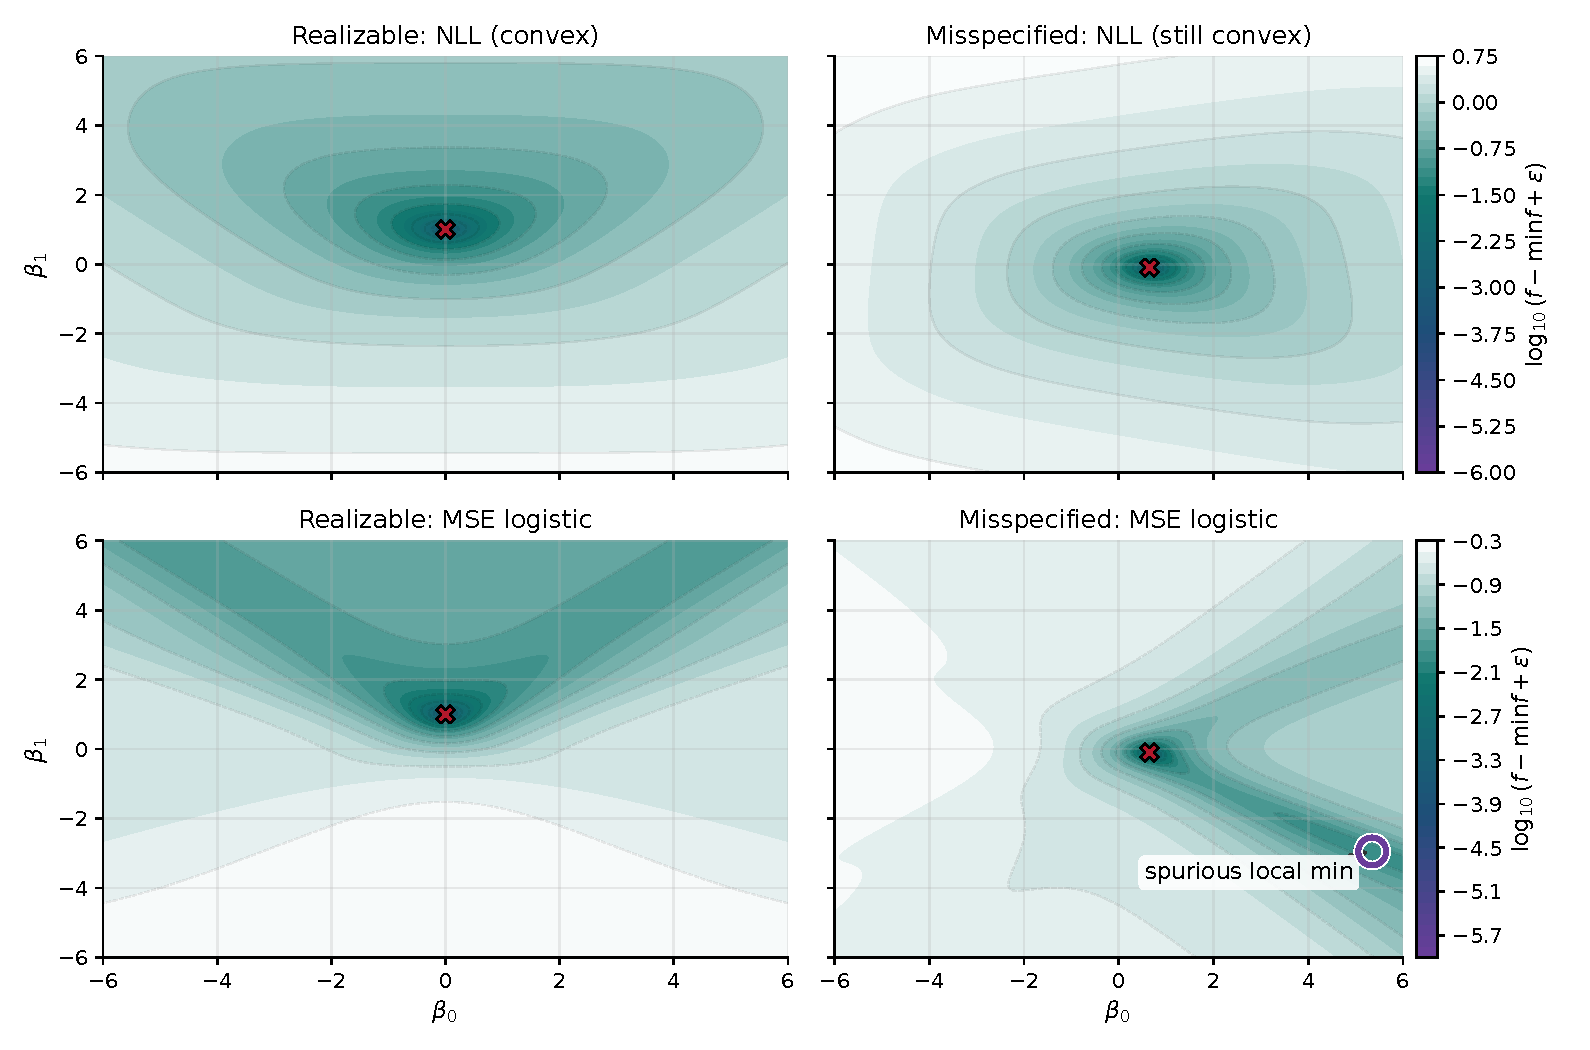
\includegraphics[width=\textwidth]{figures/handouts/convexity_optimization/fig_logistic_landscape_2d}
  \caption{A consistent contourf view of logistic landscapes in a 2D parameterization $\beta=(\beta_0,\beta_1)$.
  The plots show $\log_{10}(f-\min f+\varepsilon)$ for each objective, which makes basins comparable across panels.
  The red X marker indicates the global minimizer in each panel; in the bottom-right plot, the circled point is a spurious local minimum.
  In this example, the NLL landscape is unimodal in both realizable and misspecified settings, while the squared-loss landscape can develop extra basins under misspecification.}
  \label{fig:logistic-landscape-2d}
\end{figure}

% ------------------------------------------------------------
Example~I separates three distinct regimes.
Empirical MSE-logistic can create spurious basins; the realizable population risk has no spurious local minima but can still be slow because of broad plateaus; and misspecification can bring back genuinely wrong stable basins.
The response depends on the regime: use a stable objective when possible, use damping or line search when curvature is unreliable, and use restarts or stronger initializations when multiple basins are present.

% ------------------------------------------------------------
\section[Example II (phase retrieval)]{Example II: multimodality from symmetry, but only global optima in phase retrieval}
\label{sec:phase-retrieval}

In coherent diffraction imaging, optics, and astronomy, sensors measure intensities and lose phase.
A canonical real model is \emph{phase retrieval}:
\[
y_i = (a_i^\top x^\star)^2,\qquad i=1,\dots,m,
\]
where $x^\star\in\R^d$ is the unknown signal and $a_i$ are known sensing vectors.
A standard nonconvex least-squares objective is
\begin{equation}
F(x)=\frac{1}{4m}\sum_{i=1}^m\big((a_i^\top x)^2 - y_i\big)^2.
\label{eq:phase-empirical}
\end{equation}
This objective is nonconvex for structural reasons (it involves squares of linear forms),
and it is \emph{inherently} multimodal because $x^\star$ and $-x^\star$ generate the same data.

Like squared-loss logistic regression, phase retrieval is a smooth, nonconvex least-squares objective.
But here the nonconvexity is driven primarily by a \emph{symmetry}: $x^\star$ and $-x^\star$ generate the same data.
In population (for Gaussian designs), this symmetry produces multiple global optima but \emph{no} suboptimal local minima; the remaining stationary points are saddles.
This is ``benign'' nonconvexity (a strict-saddle picture), and it contrasts with ecological logistic regression (\Cref{sec:ecological-logistic}), where aggregation creates intrinsic nonconvexity and can lead to many distinct basins.
This ``benign geometry'' picture (multiple equivalent global minimizers; strict saddles elsewhere) appears broadly in modern tractable nonconvex problems; see \citet[\S2]{sun_qu_wright_2015_nonconvex_not_scary} and \citet[\S1]{zhang_qu_wright_2020_symmetry_geometry}.

\begin{figure}[t]
  \centering
  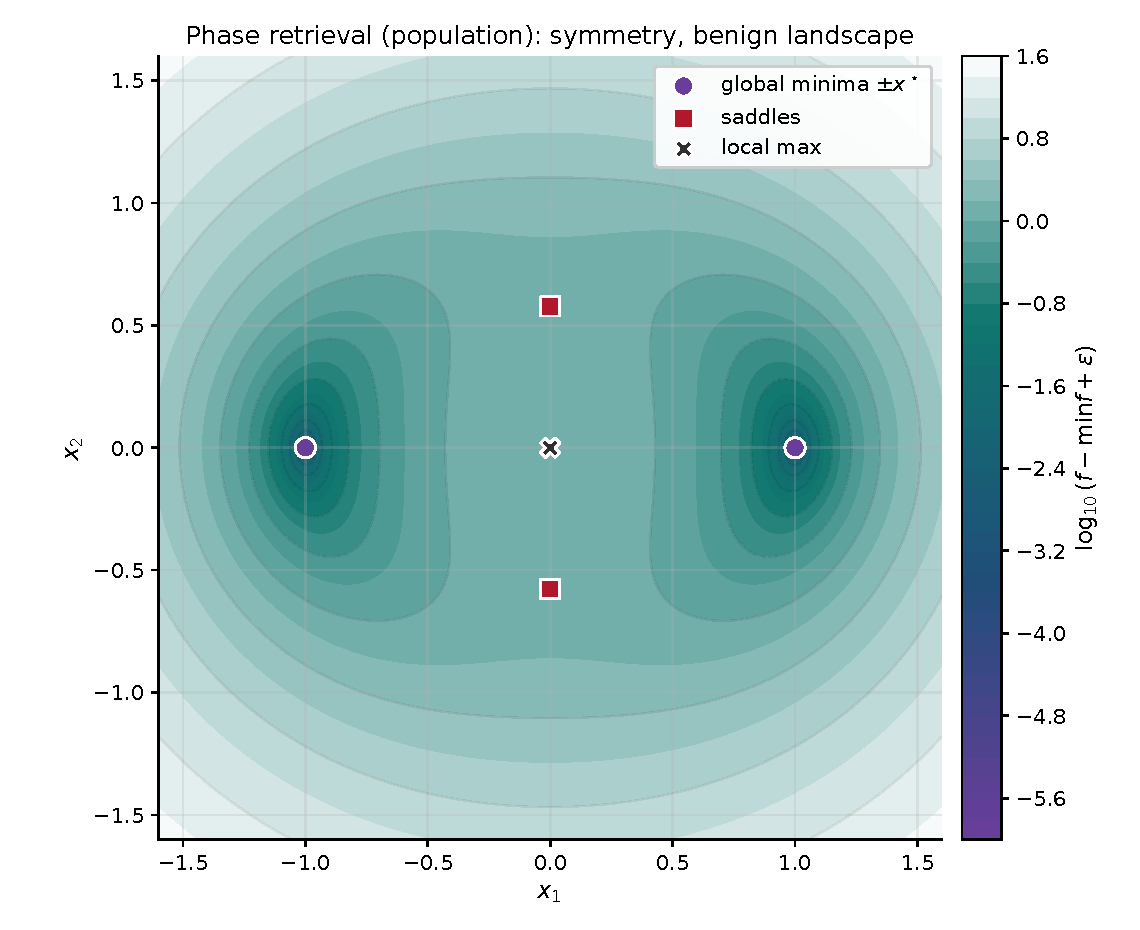
\includegraphics[width=0.86\textwidth]{figures/handouts/convexity_optimization/fig_phase_retrieval_landscape}
  \caption{Population phase retrieval in $d=2$: the landscape is nonconvex and symmetric ($x\sim -x$), but the only local minima are the two global minima $\pm x^\star$; other critical points are saddles or a local maximum at the origin.}
  \label{fig:phase-retrieval-landscape}
\end{figure}

For a clean population model, assume $a\sim N(0,I_d)$ and consider the \emph{population} objective
\begin{equation}
  f(x)=\frac12\,\E\Big[\big((a^\top x)^2 - (a^\top x^\star)^2\big)^2\Big].
  \label{eq:phase-pop}
\end{equation}

\begin{proposition}[Population phase retrieval: nonconvex but no spurious local minima]
\label{prop:phase-retrieval-benign}
For $f$ in \eqref{eq:phase-pop},
\begin{equation}
  f(x)
  =\frac{3}{2}\norm{x}^4 - \norm{x}^2\norm{x^\star}^2 - 2\ip{x}{x^\star}^2 + \frac{3}{2}\norm{x^\star}^4,
  \label{eq:phase-pop-closed-form}
\end{equation}
and the stationary points are:
\begin{enumerate}[leftmargin=*]
  \item global minima $x=\pm x^\star$ (value $0$),
  \item a local maximum at $x=0$,
  \item a saddle set $\{x:\ x\perp x^\star,\ \norm{x}=\norm{x^\star}/\sqrt{3}\}$.
\end{enumerate}
In particular, every local minimum is global.
\end{proposition}

\begin{exercise}[Phase retrieval: derive and classify the population stationary points]
\label{ex:phase-pop-derivation}
Prove \Cref{prop:phase-retrieval-benign}.
\begin{enumerate}[leftmargin=*]
  \item Expand \eqref{eq:phase-pop} and use the Gaussian fourth-moment identities
  \[
  \E[(a^\top u)^4]=3\norm{u}^4,
  \qquad
  \E[(a^\top u)^2(a^\top v)^2]=\norm{u}^2\norm{v}^2 + 2\ip{u}{v}^2,
  \]
  to obtain \eqref{eq:phase-pop-closed-form}.
  \item Differentiate \eqref{eq:phase-pop-closed-form} to get an explicit formula for $\nabla f(x)$.
  \item Solve $\nabla f(x)=0$ by decomposing $x=\alpha x^\star + u$ with $u\perp x^\star$.
  \item Classify the stationary points as global minima, a local maximum, and a saddle set.
\end{enumerate}
\end{exercise}

\SolutionBox[22]{%
\emph{Part (1) (closed form).}
Expanding the square in \eqref{eq:phase-pop} gives
\[
f(x)
=\frac12\,\E\big[(a^\top x)^4\big]
\;-\;\E\big[(a^\top x)^2(a^\top x^\star)^2\big]
\;+\;\frac12\,\E\big[(a^\top x^\star)^4\big].
\]
Apply the stated Gaussian fourth-moment identities with $u=x$ and $v=x^\star$ to get
\[
\E[(a^\top x)^4]=3\norm{x}^4,\qquad
\E[(a^\top x^\star)^4]=3\norm{x^\star}^4,
\]
and
\[
\E[(a^\top x)^2(a^\top x^\star)^2]=\norm{x}^2\norm{x^\star}^2 + 2\ip{x}{x^\star}^2.
\]
Substituting yields \eqref{eq:phase-pop-closed-form}.

\emph{Part (2) (gradient).}
Differentiate \eqref{eq:phase-pop-closed-form}:
\[
\nabla f(x)
= 6\norm{x}^2 x - 2\norm{x^\star}^2 x - 4\ip{x}{x^\star}x^\star
= (6\norm{x}^2-2\norm{x^\star}^2)x - 4\ip{x}{x^\star}x^\star.
\]

\emph{Part (3) (stationary points).}
Let $r=\norm{x^\star}_2$ and decompose $x=\alpha x^\star + u$ with $u\perp x^\star$.
Then $\ip{x}{x^\star}=\alpha r^2$ and $\norm{x}^2=\alpha^2r^2+\norm{u}^2$.
Setting $\nabla f(x)=0$ and matching the $u$ and $x^\star$ components gives
\[
(6\norm{x}^2-2r^2)\,u=0,
\qquad
\alpha\,(6\norm{x}^2-6r^2)=0.
\]
If $u=0$, then either $\alpha=0$ (so $x=0$) or $\norm{x}^2=r^2$ (so $\alpha=\pm 1$ and $x=\pm x^\star$).
If $u\neq 0$, then the first equation forces $\norm{x}^2=r^2/3$, and the second forces $\alpha=0$, hence
$x\perp x^\star$ and $\norm{x}=r/\sqrt{3}$.
This gives exactly the stationary-point list in \Cref{prop:phase-retrieval-benign}.

\emph{Part (4) (classification).}
Since $f$ in \eqref{eq:phase-pop} is an expectation of a square, $f(x)\ge 0$ for all $x$.
Also $f(\pm x^\star)=0$, so $\pm x^\star$ are global minima.

For $x=0$, the expansion \eqref{eq:phase-pop-closed-form} shows
\[
f(0)-f(x)= r^2\norm{x}^2 + 2\ip{x}{x^\star}^2 - \frac{3}{2}\norm{x}^4,
\]
which is strictly positive for all sufficiently small $x\neq 0$ (the quadratic term dominates), so $x=0$ is a local maximum.

Finally, if $x\perp x^\star$ and $\norm{x}=r/\sqrt{3}$, then the univariate restriction $t\mapsto f(x+t x^\star)$ has negative second derivative at $t=0$, so there is a direction of negative curvature.
Hence these points are saddles, and every local minimum is global.%
}

This is symmetry-driven nonconvexity with a strict-saddle geometry:
every non-optimal stationary point has a direction of negative curvature.

Phase retrieval is typically approached via the two-stage template in \Cref{alg:two-stage-template}:
use a cheap global initializer, then run a local method.
In the Gaussian model, there is a clean way to build a provably good direction estimate from a simple moment identity.
Assume the noiseless Gaussian design model $a_i \stackrel{\mathrm{iid}}{\sim} N(0,I_d)$ with measurements $y_i=(a_i^\top x^\star)^2$.
Define the \emph{spectral matrix}
\[
  Y = \frac{1}{m}\sum_{i=1}^m y_i a_i a_i^\top.
\]
Also define the radius estimate
\[
  \hat r^2 = \frac{1}{m}\sum_{i=1}^m y_i,
\]
which satisfies $\E[\hat r^2]=\norm{x^\star}_2^2$.
If $\hat u$ is a unit-norm top eigenvector of $Y$, then the standard spectral initializer is $x^{(0)}=\hat r\,\hat u$.

The next proposition explains why this initialization is reasonable.
It shows that (i) the population matrix $\E[Y]$ has a unique leading eigenvector in the $x^\star$ direction, and (ii) if the empirical $Y$ is close to $\E[Y]$ in operator norm then its leading eigenvector must be close to $\pm x^\star/\norm{x^\star}_2$.
(Here $\norm{M}_{\mathrm{op}}$ denotes the operator norm, i.e.\ the largest absolute eigenvalue for a symmetric matrix $M$.)

\begin{proposition}[Gaussian phase retrieval: why the spectral initializer points at $x^\star$]
\label{prop:phase-spectral-init}
Assume $x^\star\neq 0$, let $a\sim N(0,I_d)$, and set $y=(a^\top x^\star)^2$.
Write $r=\norm{x^\star}_2$ and $u^\star=x^\star/r$.
Define the population matrix
\[
  Y_{\mathrm{pop}} = \E\big[y\,a a^\top\big]
  = \E\big[(a^\top x^\star)^2 a a^\top\big].
\]
Then
\[
  Y_{\mathrm{pop}}=r^2 I_d + 2x^\star(x^\star)^\top,
\]
so the unique leading eigenvector of $Y_{\mathrm{pop}}$ is $u^\star$.
Moreover, if $Y$ is any symmetric matrix satisfying
\[
\norm{Y-Y_{\mathrm{pop}}}_{\mathrm{op}} \le \varepsilon\, r^2
\qquad\text{for some }\varepsilon\in(0,1),
\]
then for every unit-norm leading eigenvector $\hat u$ of $Y$ there exists a sign $s\in\{\pm 1\}$ such that
$\norm{\hat u-su^\star}_2\le \sqrt{2\varepsilon}$.
\end{proposition}

\begin{exercise}[Phase retrieval: why spectral initialization points at $x^\star$]
\label{ex:phase-spectral-spike}
Prove \Cref{prop:phase-spectral-init}.
Conclude that if the empirical matrix $Y$ is close to $Y_{\mathrm{pop}}$ in operator norm, then its top eigenvector is close to $\pm u^\star$ and the spectral initializer $x^{(0)}=\hat r\,\hat u$ is close to $\pm x^\star$.
\emph{Hint:} to compute $Y_{\mathrm{pop}}$, you can either compute entries using the Gaussian fourth-moment identity
$\E[a_i a_j a_k a_\ell]=\delta_{ij}\delta_{k\ell}+\delta_{ik}\delta_{j\ell}+\delta_{i\ell}\delta_{jk}$,
or compute the entries directly by expanding.
For the perturbation bound, compare quadratic forms $v^\top Y v$ and use $|v^\top (Y-Y_{\mathrm{pop}}) v|\le \norm{Y-Y_{\mathrm{pop}}}_{\mathrm{op}}$ for unit $v$.
Finally, explain in a sentence why one expects $\norm{Y-Y_{\mathrm{pop}}}_{\mathrm{op}}$ to be small when $m$ is large in the Gaussian model.
\end{exercise}

\SolutionBox[20]{%
Write $u=x^\star$ and expand $y=(a^\top u)^2=\sum_{k,\ell} u_k u_\ell a_k a_\ell$.
For each entry $(i,j)$,
\[
\E\!\big[y\,a_i a_j\big]
=\sum_{k,\ell} u_k u_\ell\,\E[a_i a_j a_k a_\ell]
=\sum_{k,\ell} u_k u_\ell\bigl(\delta_{ij}\delta_{k\ell}+\delta_{ik}\delta_{j\ell}+\delta_{i\ell}\delta_{jk}\bigr).
\]
The first term gives $\delta_{ij}\sum_k u_k^2=\delta_{ij}\norm{u}_2^2$.
The second and third terms each give $u_i u_j$.
Thus $\E[y\,a_i a_j]=\norm{u}_2^2\,\delta_{ij}+2u_i u_j$, i.e.
$Y_{\mathrm{pop}}=\norm{u}_2^2 I_d + 2uu^\top$.

For eigenvalues, note that $Y_{\mathrm{pop}}u=(\norm{u}_2^2+2\norm{u}_2^2)u=3\norm{u}_2^2 u$.
If $w\perp u$, then $uu^\top w=0$ so $Y_{\mathrm{pop}}w=\norm{u}_2^2 w$.
Hence the unique top eigenspace is $\mathrm{span}\{u\}$.

Let $r=\norm{u}_2$ and $u^\star=u/r$.
Let $\hat u$ be a unit top eigenvector of $Y$.
Write $E=Y-Y_{\mathrm{pop}}$ and assume $\norm{E}_{\mathrm{op}}\le \varepsilon r^2$.
Then
\[
\hat u^\top Y_{\mathrm{pop}} \hat u
= \hat u^\top Y \hat u - \hat u^\top E \hat u
\ge \lambda_{\max}(Y) - \norm{E}_{\mathrm{op}}
\ge (u^\star)^\top Y u^\star - \norm{E}_{\mathrm{op}}
\ge 3r^2 - 2\varepsilon r^2.
\]
On the other hand,
$
\hat u^\top Y_{\mathrm{pop}} \hat u
= r^2 + 2r^2\,|\ip{\hat u}{u^\star}|^2.
$
Combining gives $|\ip{\hat u}{u^\star}|^2\ge 1-\varepsilon$.
Choosing the sign that maximizes the inner product,
\[
\min\{\norm{\hat u-u^\star}_2,\norm{\hat u+u^\star}_2\}^2
=2\bigl(1-|\ip{\hat u}{u^\star}|\bigr)
\le 2\bigl(1-|\ip{\hat u}{u^\star}|^2\bigr)
\le 2\varepsilon.
\]

The matrix $Y$ is an empirical average of i.i.d.\ symmetric matrices with mean $Y_{\mathrm{pop}}$.
To make this quantitative in high dimensions, one uses concentration inequalities for random matrices to bound $\norm{Y-Y_{\mathrm{pop}}}_{\mathrm{op}}$ with high probability; see \citet[\S2.2]{zhang_qu_wright_2020_symmetry_geometry} for discussion and references.
These probability tools are largely orthogonal to our focus here.%
}

Once you have an initialization that is close to $\pm x^\star$, the local stage behaves like the convex story again.
In the Gaussian population objective, $\pm x^\star$ are not only global minima: they are \emph{locally strongly convex} minima, so the standard local strong-convexity analysis from the Optimization unit gives a linear rate while the iterates remain in that neighborhood.

\begin{exercise}[Phase retrieval: local convexity near $\pm x^\star$ in the population objective]
\label{ex:phase-pop-local-strong-convex}
For the population objective $f$ in \eqref{eq:phase-pop-closed-form}, compute the Hessian $\Hess f(x)$ and show that
\[
\Hess f(x^\star)=4\norm{x^\star}_2^2 I_d + 8x^\star(x^\star)^\top.
\]
Deduce the eigenvalues of $\Hess f(x^\star)$ and interpret this as a local condition-number statement near $x^\star$.
\end{exercise}

\SolutionBox[12]{%
Differentiate the gradient formula in the solution to \Cref{ex:phase-pop-derivation}:
for $x\in\R^d$,
\[
\Hess f(x)=12xx^\top + (6\norm{x}_2^2-2\norm{x^\star}_2^2)I_d - 4x^\star(x^\star)^\top.
\]
At $x=x^\star$ this becomes
\[
\Hess f(x^\star)=(12-4)x^\star(x^\star)^\top + 4\norm{x^\star}_2^2 I_d
=8x^\star(x^\star)^\top + 4\norm{x^\star}_2^2 I_d.
\]
Along $u^\star=x^\star/\norm{x^\star}_2$ the eigenvalue is $12\norm{x^\star}_2^2$, and along any direction orthogonal to $x^\star$ the eigenvalue is $4\norm{x^\star}_2^2$.
So near $x^\star$ the population objective is well conditioned (local condition number $3$), which is exactly the regime where local methods behave like in the convex case.%
}

These pieces give the standard Gaussian-model story:
spectral initialization supplies a direction close to $\pm x^\star$, and the local geometry near $\pm x^\star$ is strongly convex, so local methods converge quickly once initialized there.
Rigorous finite-sample analyses follow this template; see \citet[\S2.2]{zhang_qu_wright_2020_symmetry_geometry} and references therein.

Phase retrieval shows a different kind of nonconvexity.
The sign symmetry creates multiple optima, but they are equivalent, and the remaining stationary points are saddles rather than bad local minima.
The right response is therefore not exhaustive global search; it is a coarse initializer, such as a spectral method, followed by local refinement inside the basin of $\pm x^\star$.



% ------------------------------------------------------------
\section[Example III (ecological logistic)]{Example III: hard nonconvexity from aggregation in ecological logistic regression}
\label{sec:ecological-logistic}

In some applications we observe covariates at the unit level but only aggregated outcomes.
For example, we might see covariates $x_{g,1},\dots,x_{g,n_g}$ for individuals in a group (a precinct, a cohort, a batch),
but instead of observing the binary outcomes $Y_{g,i}\in\{0,1\}$ we only observe the group total
\[
Z_g = \sum_{i=1}^{n_g} Y_{g,i}.
\]
Many different binary vectors $(Y_{g,1},\dots,Y_{g,n_g})$ can produce the same total $Z_g$, so the likelihood for $\beta$ must marginalize over a large discrete set of latent ``assignments.''

Assume a logistic model at the unit level:
\[
\Pr(Y_{g,i}=1\mid x_{g,i},\beta)=\sigma(x_{g,i}^\top\beta),
\qquad i=1,\dots,n_g,
\]
with conditional independence across $i$ given the covariates.
Write $p_{g,i}(\beta)=\sigma(x_{g,i}^\top\beta)$.
Then $Z_g$ is a sum of independent but non-identically distributed Bernoulli random variables (a Poisson--binomial model), and the marginal likelihood contains $\binom{n_g}{z_g}$ terms.
The resulting negative log-likelihood is typically nonconvex in $\beta$.
This combinatorial marginalization also creates a separate difficulty that is easy to miss if we focus only on the geometry:
when $n_g$ is large, the likelihood term $\Pr(Z_g=z_g\mid x_{g,1},\dots,x_{g,n_g},\beta)$ can be expensive to evaluate repeatedly inside an optimizer.
The naive computation is literally a sum over $\binom{n_g}{z_g}$ assignments (as in \Cref{ex:eco-logistic-nonconvex}), which is intractable for large groups.
This ``optimization + marginalization'' pattern is common in latent-variable models: hard landscapes and expensive objective evaluations can come together.

An empirical negative log-likelihood objective for $G$ independent groups is
\begin{equation}
  f(\beta)
  =
  -\frac{1}{G}\sum_{g=1}^G \log \Pr(Z_g=z_g \mid x_{g,1},\dots,x_{g,n_g},\beta).
  \label{eq:eco-logistic-obj}
\end{equation}
Two edge cases are instructive.
In the special case where the covariates are constant within each group ($x_{g,i}\equiv x_g$), we have
$Z_g\sim \mathrm{Binomial}(n_g,\sigma(x_g^\top\beta))$, and \eqref{eq:eco-logistic-obj} reduces to the usual convex binomial logistic-regression objective from the Optimization unit.
At the other extreme, if $d=1$ with $\beta=(\beta_0,\beta_1)$ and each group contains covariates in $\pm$ pairs (for every $x$ the value $-x$ appears with the same multiplicity), then the marginal likelihood is symmetric in the slope: it is unchanged under $\beta_1\mapsto -\beta_1$.
This kind of symmetry reflects a genuine non-identifiability from totals alone.

\begin{exercise}[Ecological logistic regression: two easy special cases]
\label{ex:eco-logistic-edge-cases}
\begin{enumerate}[leftmargin=*]
  \item Suppose $x_{g,i}\equiv x_g$ within each group.
  Show that $Z_g\sim \mathrm{Binomial}(n_g,\sigma(x_g^\top\beta))$ and conclude that the corresponding negative log-likelihood is convex in $\beta$.
  \item Assume $d=1$ with $\beta=(\beta_0,\beta_1)$ and suppose the multiset $\{x_1,\dots,x_n\}$ is symmetric: for every $x$ it contains $-x$ with the same multiplicity.
  Show that, for every $z$,
  \[
    \Pr(Z=z\mid x_1,\dots,x_n,(\beta_0,\beta_1))
    =
    \Pr(Z=z\mid x_1,\dots,x_n,(\beta_0,-\beta_1)).
  \]
  Conclude that the likelihood for $\beta_1$ is an even function, so the sign of the slope is not identifiable from $Z$ alone in such a balanced design.
\end{enumerate}
\end{exercise}

\SolutionBox[14]{%
\emph{Part (1).}
If $x_{g,i}\equiv x_g$, then conditional on $x_g$ the unit-level outcomes are i.i.d.\ Bernoulli with success probability $\sigma(x_g^\top\beta)$.
Therefore $Z_g=\sum_{i=1}^{n_g}Y_{g,i}\sim \mathrm{Binomial}(n_g,\sigma(x_g^\top\beta))$.
Up to an additive constant (independent of $\beta$), the per-group negative log-likelihood can be written as a function of the scalar $\eta=x_g^\top\beta$:
\[
\ell_g(\beta)
= -z_g\,\eta + n_g\log(1+e^\eta).
\]
Since $\frac{d^2}{d\eta^2}\ell_g(\eta)=n_g\,\sigma'(\eta)\ge 0$, the map $\eta\mapsto \ell_g(\eta)$ is convex.
Composing a convex function with a linear map $\beta\mapsto x_g^\top\beta$ preserves convexity, so $\ell_g$ is convex in $\beta$.
Summing over $g$ preserves convexity, hence the full objective is convex.

\emph{Part (2).}
Write $p_i(\beta_0,\beta_1)=\sigma(\beta_0+\beta_1 x_i)$.
Replacing $\beta_1$ by $-\beta_1$ replaces $p_i$ by $\tilde p_i=\sigma(\beta_0-\beta_1 x_i)$.
By the assumed symmetry of the multiset $\{x_i\}$, the multiset $\{\tilde p_i\}$ is the same as $\{p_i\}$ up to a permutation (each $x$ is paired with $-x$).
But the distribution of $Z=\sum_i Y_i$ depends only on the multiset of success probabilities, not on how they are ordered, so $\Pr(Z=z\mid x_1,\dots,x_n,(\beta_0,\beta_1))=\Pr(Z=z\mid x_1,\dots,x_n,(\beta_0,-\beta_1))$ for every $z$.
Thus the likelihood is an even function of $\beta_1$, which means the sign of the slope is not identifiable from totals in this balanced design.%
}

This example ties directly to the empirical-versus-population theme from Example~I.
There the bad basins can be a finite-sample artifact under benign population geometry; here the nonconvexity is intrinsic, because even under the correct model and infinite data aggregation forces us to marginalize over discrete latent assignments.
That marginalization step is also the bridge to the Expectation--maximization subsection of the Augmented-state optimization unit: once the assignments are latent, the natural algorithmic object is the EM update map, which alternates exact conditional expectations with parameter updates, rather than a single closed-form convex objective.

To emphasize this, it is useful to look at a \emph{population} version of \eqref{eq:eco-logistic-obj}.
Let $X=(x_1,\dots,x_n)$ denote a random group of covariates and let $Z$ be generated from the model under a true parameter $\beta^\star$.
Define the population objective
\[
F(\beta)=\E\big[-\log \Pr(Z\mid X,\beta)\big].
\]
Because the model is correctly specified, $F$ is minimized at (an observationally equivalent version of) $\beta^\star$.
However, as \Cref{fig:eco-logistic-pop-landscape} illustrates, $F$ can still have multiple separated basins and spurious local minima.

\begin{figure}[H]
  \centering
  \input{figures/handouts/convexity_optimization/fig_ecological_logistic_population_landscape}
  \caption{A toy \emph{population} objective for ecological logistic regression in a 2D parameterization $\beta=(\beta_0,\beta_1)$.
  Each group has $n=6$ units and is equally likely to have covariates $(-4,-3,-2,2,3,4)$, $(-3,-1,1,2,3,4)$, or $(-2,-1,1,2,3,4)$ (in $d=1$); outcomes are generated under $\beta^\star=(0.3,1.2)$.
  The plot shows $\log_{10}(F-\min F+\varepsilon)$, as in \Cref{fig:logistic-landscape-2d}; the red X marks $\beta^\star$ and the open circles mark three spurious local minima in this toy example.}
  \label{fig:eco-logistic-pop-landscape}
\end{figure}

\begin{exercise}[Ecological logistic regression: marginalization and nonconvexity]
\label{ex:eco-logistic-nonconvex}
Fix one group with covariates $x_1,\dots,x_n\in\R^d$ and observe $Z=z$.
Let $p_i(\beta)=\sigma(x_i^\top\beta)$.
\begin{enumerate}[leftmargin=*]
  \item Show that
  \[
    \Pr(Z=z\mid x_1,\dots,x_n,\beta)
    =
    \sum_{\substack{S\subseteq\{1,\dots,n\}\\|S|=z}}
    \ \prod_{i\in S} p_i(\beta)\prod_{j\notin S}\bigl(1-p_j(\beta)\bigr).
  \]
  Interpret this as summing over all ways to choose which $z$ units are the successes.
  \item Specialize to $n=2$ and $z=1$ in $d=1$ with covariates $x_1=a$ and $x_2=b$.
  Let $\ell(\beta)$ be the negative log-likelihood $-\log \Pr(Z=1\mid a,b,\beta)$ with no regularization.
  Show that $\ell''(0)=\tfrac12 ab$.
  Conclude that $\ell$ is not convex whenever $ab<0$.
\end{enumerate}
\end{exercise}

\SolutionBox[20]{%
\emph{Part (1).}
Condition on the covariates.
For any binary vector $y=(y_1,\dots,y_n)\in\{0,1\}^n$, conditional independence gives
\[
\Pr(Y_1=y_1,\dots,Y_n=y_n\mid x_1,\dots,x_n,\beta)
=
\prod_{i=1}^n p_i(\beta)^{y_i}\bigl(1-p_i(\beta)\bigr)^{1-y_i}.
\]
The event $\{Z=z\}$ is the union of all assignments $y$ with exactly $z$ ones, so summing over those assignments yields
\[
\Pr(Z=z\mid x_1,\dots,x_n,\beta)
=
\sum_{\substack{y\in\{0,1\}^n\\ \sum_i y_i=z}}
\ \prod_{i=1}^n p_i(\beta)^{y_i}\bigl(1-p_i(\beta)\bigr)^{1-y_i}.
\]
Reindexing the sum by the subset $S=\{i:\ y_i=1\}$ (which has $|S|=z$) gives the stated formula.

\emph{Part (2).}
For $n=2$ and $z=1$, let $p_1(\beta)=\sigma(a\beta)$ and $p_2(\beta)=\sigma(b\beta)$.
Then
\[
q(\beta)=\Pr(Z=1\mid a,b,\beta)
 = p_1(1-p_2) + (1-p_1)p_2
 = p_1+p_2-2p_1p_2,
\]
and $\ell(\beta)=-\log q(\beta)$.
At $\beta=0$ we have $p_1=p_2=\tfrac12$, so $q(0)=\tfrac12$.
Also $p_1'(\beta)=a\,p_1(1-p_1)$ and $p_2'(\beta)=b\,p_2(1-p_2)$, so $p_1'(0)=a/4$ and $p_2'(0)=b/4$.
A direct differentiation gives $q'(0)=0$ and
\[
q''(0)=-4p_1'(0)p_2'(0)=-4\cdot\frac{a}{4}\cdot\frac{b}{4}=-\frac{ab}{4}.
\]
Since $\ell'=-q'/q$ and $q'(0)=0$, we have $\ell''(0)=-(q''(0)/q(0))$ and therefore
\[
\ell''(0)
=-\frac{q''(0)}{q(0)}
=-\frac{-ab/4}{1/2}
=\frac{ab}{2}.
\]
If $ab<0$, then $\ell''(0)<0$, so $\ell$ is not convex.
}

Even though the landscape can be globally hard (and even the population objective can have spurious basins, as in \Cref{fig:eco-logistic-pop-landscape}), there is still a familiar ``convex'' story \emph{locally} around the true parameter under correct specification.
When the model is locally identifiable, the population objective has a neighborhood of $\beta^\star$ on which it is convex (indeed strongly convex).
One convenient way to see this in ecological logistic regression is to expose the probabilistic structure behind the gradient and Hessian: the observed-data objective involves marginalizing over latent assignments, and its Hessian can be written as a difference of two covariance matrices.
After averaging over the random total $Z$ under the true model, that difference becomes a covariance by the law of total covariance.

\begin{exercise}[Ecological logistic regression: DC structure and local convexity near $\beta^\star$]
\label{ex:eco-logistic-pop-local-convex}
Fix covariates $x_1,\dots,x_n\in\R^d$.
For $\beta\in\R^d$, let $V_1,\dots,V_n$ be independent Bernoulli random variables with
\[
\Pr(V_j=1\mid x_j,\beta)=\sigma(x_j^\top\beta),
\qquad j=1,\dots,n,
\]
and define
\[
U = \sum_{j=1}^n x_j V_j,
\qquad
Z = \sum_{j=1}^n V_j.
\]
For an observed total $Z=z$, write $L_z(\beta)=-\log \Pr(Z=z\mid x_1,\dots,x_n,\beta)$.
\begin{enumerate}[leftmargin=*]
  \item Show the \emph{difference-of-convex (DC)} form
  \[
  L_z(\beta)
  =\sum_{j=1}^n \log\bigl(1+e^{x_j^\top\beta}\bigr)
  -\log\left(\sum_{\substack{S\subseteq\{1,\dots,n\}\\|S|=z}} \exp\Big(\sum_{j\in S} x_j^\top\beta\Big)\right).
  \]
  \item Show that $\nabla L_z(\beta)=\E[U]-\E[U\mid Z=z]$.
  \item Show that $\Hess L_z(\beta)=\mathrm{Cov}(U)-\mathrm{Cov}(U\mid Z=z)$.
  (Hint: for $g(\beta)=\log\sum_k e^{a_k^\top\beta}$, the Hessian is the covariance of the vectors $\{a_k\}$ under the corresponding softmax weights.)
  \item Consider the population objective $F(\beta)=\E[L_Z(\beta)]$ when $Z$ is generated under a true parameter $\beta^\star$.
  Assuming the outer expectation defining $F$ can be differentiated twice under the integral sign, use the conditional law of total covariance,
  \[
    \mathrm{Cov}(U\mid X)=\E[\mathrm{Cov}(U\mid Z,X)\mid X] + \mathrm{Cov}(\E[U\mid Z,X]\mid X),
  \]
  to show that
  \[
    \E\big[\Hess L_Z(\beta^\star)\mid X\big]
    = \mathrm{Cov}\big(\E[U\mid Z,X]\mid X\big)\succeq 0.
  \]
  Deduce that
  \[
    \Hess F(\beta^\star)
    = \E\Big[\mathrm{Cov}\big(\E[U\mid Z,X]\mid X\big)\Big]\succeq 0.
  \]
  Conclude that if $\Hess F(\beta^\star)\succ 0$, then $F$ is locally strongly convex on a neighborhood of $\beta^\star$.
\end{enumerate}
\end{exercise}

\SolutionBox[22]{%
\emph{Part (1).}
Write $\eta_j=x_j^\top\beta$ and $p_j=\sigma(\eta_j)=e^{\eta_j}/(1+e^{\eta_j})$.
For any subset $S$ with $|S|=z$,
\[
\Pr(V_j=1\ \forall j\in S,\ V_j=0\ \forall j\notin S\mid x_1,\dots,x_n,\beta)
=\prod_{j\in S}p_j\prod_{j\notin S}(1-p_j)
=\frac{\exp(\sum_{j\in S}\eta_j)}{\prod_{j=1}^n(1+e^{\eta_j})}.
\]
Summing over all $S$ with $|S|=z$ gives
\[
\Pr(Z=z\mid x_1,\dots,x_n,\beta)
=\frac{\sum_{|S|=z}\exp(\sum_{j\in S}\eta_j)}{\prod_{j=1}^n(1+e^{\eta_j})}.
\]
Taking $-\log$ yields the stated DC representation.

\emph{Parts (2) and (3).}
The first term in $L_z$ has gradient $\sum_j \sigma(\eta_j)x_j$ and Hessian $\sum_j \sigma'(\eta_j)x_jx_j^\top$.
Since $U=\sum_j x_j V_j$ with independent Bernoulli coordinates, these are exactly $\E[U]$ and $\mathrm{Cov}(U)$.

For the second term, define a probability distribution on subsets $S$ of size $z$ by
\[
w_S(\beta)\propto \exp\Big(\sum_{j\in S}x_j^\top\beta\Big),
\qquad |S|=z.
\]
This is the conditional law of the success set $\{j:\ V_j=1\}$ given $Z=z$ under parameter $\beta$.
Therefore
\[
\nabla \log\Big(\sum_{|S|=z} e^{\sum_{j\in S}x_j^\top\beta}\Big)
  = \sum_{|S|=z} w_S(\beta)\sum_{j\in S}x_j
  = \E[U\mid Z=z],
\]
and differentiating once more gives
\[
\Hess\!\left(\log\Big(\sum_{|S|=z} e^{\sum_{j\in S}x_j^\top\beta}\Big)\right)
=\mathrm{Cov}(U\mid Z=z),
\]
which yields $\nabla L_z=\E[U]-\E[U\mid Z=z]$ and $\Hess L_z=\mathrm{Cov}(U)-\mathrm{Cov}(U\mid Z=z)$.

\emph{Part (4).}
Now let $X=(x_1,\dots,x_n)$ be random, and assume we may differentiate the outer expectation in $F(\beta)=\E[L_Z(\beta)]$ twice under the integral sign.
Conditional on $X$ and at $\beta^\star$, take expectations over $Z$:
\[
\E\big[\Hess L_Z(\beta^\star)\mid X\big]
=\mathrm{Cov}(U\mid X)-\E[\mathrm{Cov}(U\mid Z,X)\mid X].
\]
By the conditional law of total covariance,
\[
\mathrm{Cov}(U\mid X)
=\E[\mathrm{Cov}(U\mid Z,X)\mid X] + \mathrm{Cov}(\E[U\mid Z,X]\mid X),
\]
so the difference is
\[
\E\big[\Hess L_Z(\beta^\star)\mid X\big]
=\mathrm{Cov}(\E[U\mid Z,X]\mid X)\succeq 0.
\]
Taking outer expectations gives
\[
\Hess F(\beta^\star)
=\E\big[\Hess L_Z(\beta^\star)\big]
=\E\Big[\mathrm{Cov}(\E[U\mid Z,X]\mid X)\Big]\succeq 0.
\]
If this unconditional Hessian is positive definite, then by continuity of $\Hess F$ there exists a radius $r>0$ such that $\Hess F(\beta)\succeq \tfrac12 \Hess F(\beta^\star)\succ 0$ on $\{\beta:\ \norm{\beta-\beta^\star}_2\le r\}$, which implies local strong convexity of $F$ on that neighborhood.%
}

This example still fits the two-stage template in \Cref{alg:two-stage-template}, but the coarse stage is less structured.
In practice, one often uses multiple random starts or a warm start from a crude convex surrogate, then runs a local optimizer with line search or damping on the true nonconvex objective \eqref{eq:eco-logistic-obj} and keeps the best solution found.

Ecological logistic regression is the genuinely hard case in this note.
Aggregation forces a sum over latent assignments, so the objective can have many distinct basins even under correct specification.
The practical response is usually robust search rather than a single clever local method: several starts, warm starts from crude convex surrogates when available, and then local refinement with damping or line search on the true objective.



% ------------------------------------------------------------
\section{Diagnosing nonconvex objectives}
\label{sec:checklist-streamlined}

``Nonconvex'' is not a single regime.
Squared-loss logistic regression is close to convex: the empirical objective can have spurious minima, yet under realizability the population geometry is benign and locally strongly convex near $\beta^\star$.
Phase retrieval is symmetry-driven: there can be multiple equivalent optima but no bad local minima.
Ecological logistic regression is intrinsically hard because aggregation induces latent assignments and the resulting marginal likelihood can have many distinct basins.
The right response depends on which regime you are in: stable objectives when available, spectral or other coarse initialization when symmetry is the issue, and restarts or stronger surrogates when aggregation drives the hardness.
This is also the lens used in the Expectation--maximization subsection of the Augmented-state optimization unit: the basin picture remains central, but the relevant geometry is now the geometry of the EM operator and its population/sample perturbations.

A useful diagnosis is to ask whether the difficulty comes from finite-sample noise or the population model, from symmetry or non-identifiability, from genuinely suboptimal basins, from the lack of a global guarantee beyond convexity, or simply from poor local conditioning.
Carried back to the main notes, the point is not that nonconvexity is uniformly hopeless.
The real question is which part of the convex story breaks first: the basin structure, the conditioning inside a good basin, or only the finite-sample objective we happen to optimize.

\begin{table}[t]
  \centering
  \small
  \setlength{\tabcolsep}{4pt}
  \begin{tabular}{@{}p{0.18\textwidth}p{0.24\textwidth}p{0.26\textwidth}p{0.24\textwidth}@{}}
    \toprule
    Example & Source of nonconvexity & Global geometry & Typical response \\
    \midrule
    Logistic: NLL vs MSE & objective choice + assumptions & spurious basins can appear empirically/misspecified; realizable population is benign but can be flat & pick a stable objective (NLL), add damping/restarts, check misspecification \\
    Phase retrieval & symmetry ($x\sim -x$) & strict-saddle population landscape; only local minima are global & spectral init + local refinement; perturb/noise to escape saddles \\
    Ecological\newline logistic & aggregation / missing labels & many distinct basins from latent assignments & many restarts; warm starts; keep best \\
    \bottomrule
  \end{tabular}
  \caption{Summary of the three examples by source of nonconvexity, resulting global geometry, and typical response.
  Together the columns instantiate the ``hardness = basins + geometry'' spine developed in the handout.}
  \label{tab:nonconvex-example-summary}
\end{table}

\bibliographystyle{plainnat}
\makeatletter
\begingroup
\let\input@path\@empty
\IfFileExists{references.bib}{%
  \gdef\stat221bibpath{references}%
}{%
  \IfFileExists{../references.bib}{%
    \gdef\stat221bibpath{../references}%
  }{%
    \gdef\stat221bibpath{../../references}%
  }%
}
\endgroup
\makeatother
\bibliography{\stat221bibpath}

\end{document}
"
\newif\ifshowsolutions
\showsolutionsfalse
\ifdefined\STATshowsolutions
  \showsolutionstrue
\fi
\ifcsname STAT221SOLUTIONS\endcsname
  \showsolutionstrue
\fi

% Handout-only tcolorbox style for readable title bars.
% The `stat221titlebox` tcolorbox style is defined in `Lecture Tex/preamble.tex`.

% Solution boxes (controlled by \ifshowsolutions).
% Usage: \SolutionBox{<solution body>}
\newcommand{\SolutionBox}[2][10]{%
  \ifshowsolutions
    \begin{tcolorbox}[stat221panelgray,title={Solution}]
    #2
    \end{tcolorbox}
  \else
    \begin{tcolorbox}[stat221panelgray,unbreakable,title={Workspace}]
    \vspace{#1\baselineskip}
    \end{tcolorbox}
  \fi
}

\title{When does nonconvexity make optimization hard?}
\author{}
\date{}

\begin{document}
\maketitle

\section[Nonconvexity and optimization hardness]{When does nonconvexity make optimization hard?}
\label{sec:convexity-opt-hardness-handout}

Optimization in this course starts from minimizing smooth objectives with local information: gradients, Hessians, line searches, and condition numbers describe what a descent method can see near the current iterate.
This handout asks when that local picture ceases to be the whole story once the objective is no longer convex.
The main objects are the landscape itself, the basins created by that landscape, and the local geometry that determines how quickly a method moves within a basin.

That perspective builds directly on the Optimization unit and feeds forward to the Augmented-state optimization unit, where the same basin-versus-geometry split reappears for the EM update map rather than for a single objective.
Logistic regression, phase retrieval, and ecological logistic regression then supply three contrasting regimes: an objective choice that can create misleading empirical basins, a symmetry-driven landscape with multiple equivalent optima but no bad local minima, and an intrinsically hard latent-assignment problem.

% ------------------------------------------------------------
\section[Basins and geometry]{Basins, geometry, and what local methods can promise}
\label{sec:framing-nonconvex}

Nonconvex analysis in Stat~221 still starts from the same local-method toolkit as the convex case:
\emph{smoothness} gives a descent lemma, and \emph{curvature} controls local speed.
What changes is the global question of whether the landscape contains suboptimal basins that can trap a local method away from the best achievable value.

\begin{definition}[Basic vocabulary]
\label{def:basic-vocab-nonconvex}
Let $f:\R^d\to\R$ be differentiable and write $f^\star=\inf_x f(x)$.
\begin{enumerate}[leftmargin=*]
  \item A point $x$ is a \textbf{stationary point} if $\nabla f(x)=0$.
  \item A point $x$ is a \textbf{local minimizer} if $f(x)\le f(x')$ for all $x'$ in some neighborhood of $x$.
  A local minimizer is \textbf{spurious} if $f(x)>f^\star$.
  \item A \textbf{(strict) saddle} is a stationary point $x$ with a direction of negative curvature, i.e.\ there exists $v$ such that $v^\top \Hess f(x)\,v<0$.
  \item Fix an algorithm (e.g.\ gradient descent with a specified step-size rule).
  The \textbf{basin of attraction} of a limit point $\bar x$ is the set of initializations $x^{(0)}$ for which the iterates converge to $\bar x$.
  Basins depend on the method and its hyperparameters.
\end{enumerate}
\end{definition}

In practice, local methods succeed when descent is reliable, stationary points are safe, and the initialization lands in a basin where the local geometry is favorable.
Because this is a statistical optimization class, we will repeatedly separate what comes from finite-sample randomness from what is intrinsic to the underlying model.
Concretely, we distinguish an \emph{empirical} objective (a finite-sample average) from its \emph{population} counterpart (an expectation under a model).
Spurious basins can be finite-sample artifacts, or they can persist in the population depending on the data/model assumptions.

A useful statistical trick, when an empirical landscape is messy, is to study the population objective first.
In convex optimization this is often geometry-preserving, because convexity is closed under addition: empirical averages and expectations cannot create spurious basins.
In nonconvex problems, however, the empirical and population landscapes can differ in either direction:
summing per-sample losses that are individually benign can create multiple basins, while averaging can smooth a pathological finite-sample landscape into a benign population geometry.
Making this comparison quantitative in high dimensions typically requires concentration tools (uniform convergence, operator-norm bounds), which is largely orthogonal to our focus here.

When multiple basins exist, the standard strategy is to combine a cheap coarse initializer with a local refinement stage.
The initializer is problem-specific; the local step uses the same gradient-based toolkit as in the convex setting.
\begin{algorithm}[H]
  \caption{Two-stage template: coarse initialization + local refinement}
  \label{alg:two-stage-template}
  \begin{algorithmic}[1]
    \Require Objective $f$ and its parameterization, plus whatever structure enables a cheap initializer.
    \Ensure A refined estimate $\hat\theta$ for a (near-)minimizer of $f$.
    \State \textbf{Coarse stage:} produce a small set of candidate initializations $\Theta_0$ (e.g.\ spectral/moment methods, a grid search, or a convex relaxation).
    \State Pick $\theta^{(0)}\in\Theta_0$ with the best objective value (or best surrogate score).
    \State \textbf{Local stage:} run a local optimizer (e.g.\ GD + line search, Gauss--Newton, damped Newton) starting from $\theta^{(0)}$ to obtain $\hat\theta$.
    \State Optionally repeat with multiple $\theta^{(0)}$ and keep the best solution.
  \end{algorithmic}
\end{algorithm}

% ------------------------------------------------------------
\section[Optimization hierarchy]{What properties make local methods reliable?}
\label{sec:optimization-hierarchy}

In this course we often analyze local methods (gradient descent, Newton, SGD) under assumptions like ``convex'' or ``strongly convex''; see \citep[\S9.2--9.3]{boyd_vandenberghe_2004_convex}.
Beyond convexity, there are two questions worth separating: can a local method get trapped at a suboptimal stationary point, and if it does converge, is it fast or slow because of conditioning or flat directions?

One useful ``in-between'' global condition is the Polyak--\L{}ojasiewicz (PL) inequality.
\begin{definition}[Polyak--\L{}ojasiewicz (PL) inequality]
\label{def:pl-inequality}
Let $f:\R^d\to\R$ be differentiable and let $f^\star=\inf_x f(x)$.
We say $f$ satisfies the PL inequality with parameter $\mu>0$ if for all $x\in\R^d$,
\[
\frac{1}{2}\norm{\nabla f(x)}_2^2 \ge \mu\bigl(f(x)-f^\star\bigr).
\]
\end{definition}

Every differentiable $m$-strongly convex function satisfies the PL inequality with parameter $\mu=m$, but PL can also hold even when $f$ is not convex.

\begin{proposition}[PL implies no spurious stationary points]
\label{prop:pl-no-spurious-stationary}
If $f$ satisfies the PL inequality (\Cref{def:pl-inequality}) and $\nabla f(x)=0$, then $x$ is a global minimizer of $f$.
\end{proposition}

\begin{proof}
If $\nabla f(x)=0$, then \Cref{def:pl-inequality} gives $0\ge \mu(f(x)-f^\star)$, hence $f(x)\le f^\star$.
By definition $f^\star\le f(x)$, so $f(x)=f^\star$.
\end{proof}

\begin{theorem}[Gradient descent under PL has a linear rate in function value]
\label{thm:gd-pl-linear}
Assume $f$ is $L$-smooth and satisfies the PL inequality with parameter $\mu$.
Then gradient descent with step size $1/L$ satisfies
\[
f(x^{(k)})-f^\star \le \left(1-\frac{\mu}{L}\right)^k \bigl(f(x^{(0)})-f^\star\bigr).
\]
\end{theorem}

This proof uses the same descent-lemma template developed for gradient descent in the Optimization unit.
\begin{exercise}[Gradient descent under PL]
\label{ex:gd-pl-linear}
Prove \Cref{thm:gd-pl-linear}.
\emph{Hint:} use the descent lemma for $L$-smooth functions,
\[
f\!\left(x-\frac{1}{L}\nabla f(x)\right)
\le f(x)-\frac{1}{2L}\norm{\nabla f(x)}_2^2,
\]
then apply the PL inequality (\Cref{def:pl-inequality}) and iterate.
\end{exercise}

\SolutionBox[10]{%
This is the same descent-lemma-plus-PL argument used in the Optimization unit.
By $L$-smoothness, the descent lemma gives
\[
f\!\left(x-\frac{1}{L}\nabla f(x)\right)
\le f(x)-\frac{1}{2L}\norm{\nabla f(x)}_2^2.
\]
Combine with PL to get
\[
f(x^+)-f^\star
\le f(x)-f^\star - \frac{\mu}{L}\bigl(f(x)-f^\star\bigr)
=\left(1-\frac{\mu}{L}\right)\bigl(f(x)-f^\star\bigr),
\]
and iterate.%
}

Even when convergence is guaranteed (e.g.\ under PL), conditioning still matters. The convergence rate depends on the ratio $L/\mu$, which plays the role of a condition number in \Cref{thm:gd-pl-linear}.

We now turn to three examples, each of which keeps the local-method viewpoint from the Optimization unit but changes the global landscape in a different way.
Example I (logistic regression) shows that ``nonconvex'' can still have a benign population geometry (no spurious local minima) while the empirical objective can have spurious basins and the landscape can be flat.
Example II (phase retrieval) is a clean strict-saddle example where multimodality comes from symmetry and the only local minima are global.
Example III (ecological logistic regression) is a likelihood problem with \emph{intrinsic} nonconvexity created by aggregation/partial observation: many different latent ``assignments'' can explain the same group total, so local methods can be highly initialization-dependent.

% ------------------------------------------------------------
\section[Example I (logistic)]{Example I: objective choice and data assumptions in logistic regression}
\label{sec:logistic-bridge}

In binary regression, logistic regression models
\[
\Pr(y_i=1\mid x_i,\beta)=\sigma(x_i^\top\beta),
\]
where $\sigma(z)=\frac{1}{1+e^{-z}}$ is the logistic sigmoid.
The Optimization unit introduces logistic regression through its convex negative log-likelihood and then studies the resulting gradient and Hessian formulas.
Here we keep the regression-coefficient notation $\beta$ used again in the later ecological-logistic example, and we write the convex objective as $L$ so the formulas line up with that development as closely as possible.
For comparison, we will place next to it a squared-loss objective on the predicted probabilities.
\[
L(\beta)
=
\frac{1}{n}\sum_{i=1}^n \Bigl[\log\bigl(1+e^{x_i^\top\beta}\bigr) - y_i x_i^\top \beta\Bigr]
\]
is the convex negative log-likelihood, while
\[
R_{\mathrm{sq}}(\beta)
= \frac{1}{n}\sum_{i=1}^n \bigl(y_i-\sigma(x_i^\top\beta)\bigr)^2
\]
is the squared-loss alternative.
Equivalently, one can write the pair of objectives as
\begin{enumerate}[leftmargin=*]
  \item the convex negative log-likelihood from maximum likelihood, matching the logistic-regression model developed in the Optimization unit:
  \begin{equation}
    \begin{aligned}
      L(\beta)
      &=
      -\frac{1}{n}\sum_{i=1}^n \Bigl[y_i\log \sigma(x_i^\top\beta) + (1-y_i)\log \sigma(-x_i^\top\beta)\Bigr] \\
      &=
      \frac{1}{n}\sum_{i=1}^n \Bigl[\log\bigl(1+e^{x_i^\top\beta}\bigr) - y_i x_i^\top \beta\Bigr].
    \end{aligned}
    \label{eq:logistic-nll}
  \end{equation}
  \item the squared loss on predicted probabilities, also called Brier or calibration loss, which is smooth but generally nonconvex:
  \begin{equation}
    R_{\mathrm{sq}}(\beta)
    = \frac{1}{n}\sum_{i=1}^n \bigl(y_i-\sigma(x_i^\top\beta)\bigr)^2.
    \label{eq:logistic-mse}
\end{equation}
\end{enumerate}

The three logistic regimes that matter here are finite-sample spurious minima, a realizable population landscape with no spurious local minima but broad plateaus, and misspecification, where wrong basins can return even at the population level.

For the convex logistic model from the Optimization unit, the objective $L$ in \eqref{eq:logistic-nll} has a weighted-Gram Hessian and is convex.
In particular, if $X\in\R^{n\times d}$ has rows $x_i^\top$ and $p_i(\beta)=\sigma(x_i^\top\beta)$, then
\begin{equation}
  \Hess L(\beta)
  =\frac{1}{n}X^\top W(\beta)\,X,
  \qquad
  W(\beta)=\mathrm{diag}\bigl(p_i(\beta)(1-p_i(\beta))\bigr)\succeq 0,
  \label{eq:logistic-nll-hess}
\end{equation}
so $L$ is convex.
This is the same Hessian identity proved in the Optimization unit's logistic-regression development, so we will reuse that derivation here and focus on what changes under squared loss.

By contrast, $R_{\mathrm{sq}}$ is smooth but generally nonconvex, and it can have \emph{spurious} local minima at the empirical (finite-sample) level.

To see where the nonconvexity comes from, write $z_i=x_i^\top\beta$ and recall
$\sigma'(z)=\sigma(z)(1-\sigma(z))$ and $\sigma''(z)=\sigma'(z)(1-2\sigma(z))$.
For the empirical squared loss,
\[
\nabla R_{\mathrm{sq}}(\beta)
=\frac{2}{n}\sum_{i=1}^n \bigl(\sigma(z_i)-y_i\bigr)\,\sigma'(z_i)\,x_i,
\]
and differentiating again gives
\[
\Hess R_{\mathrm{sq}}(\beta)
=\frac{2}{n}\sum_{i=1}^n\Big(\sigma'(z_i)^2 + \bigl(\sigma(z_i)-y_i\bigr)\sigma''(z_i)\Big)x_ix_i^\top.
\]
The key observation is that $\sigma''(z)$ changes sign, so the scalar coefficient in parentheses can be negative.
Thus $\Hess R_{\mathrm{sq}}(\beta)$ can be indefinite, and the objective can be nonconvex even though it is smooth.

\begin{example}[Empirical squared-loss logistic regression can have a spurious local minimum]
\label{ex:logistic-empirical-spurious}
Consider $q_\beta(x)=\sigma(x^\top\beta)$ with $\beta\in\R^2$, and the dataset
\[
((x_i,y_i))_{i=1}^8
=\Bigl(
\begin{aligned}[t]
&((-0.54,1.57),0),\ ((0.15,2.62),1),\ ((-0.89,0.66),0),\\
&((-0.22,0.64),0),\ ((-0.01,-0.64),1),\ ((-0.99,3.48),1),\\
&((-0.09,-2.29),1),\ ((-0.74,0.77),1)
\end{aligned}
\Bigr).
\]
The logistic NLL $L$ is convex by \Cref{eq:logistic-nll-hess}, but the squared-loss objective $R_{\mathrm{sq}}$ in \eqref{eq:logistic-mse} has multiple basins, including a suboptimal local minimizer.
See \Cref{fig:logistic-empirical-spurious,fig:logistic-empirical-basins}.
\end{example}

\begin{figure}[t]
  \centering
  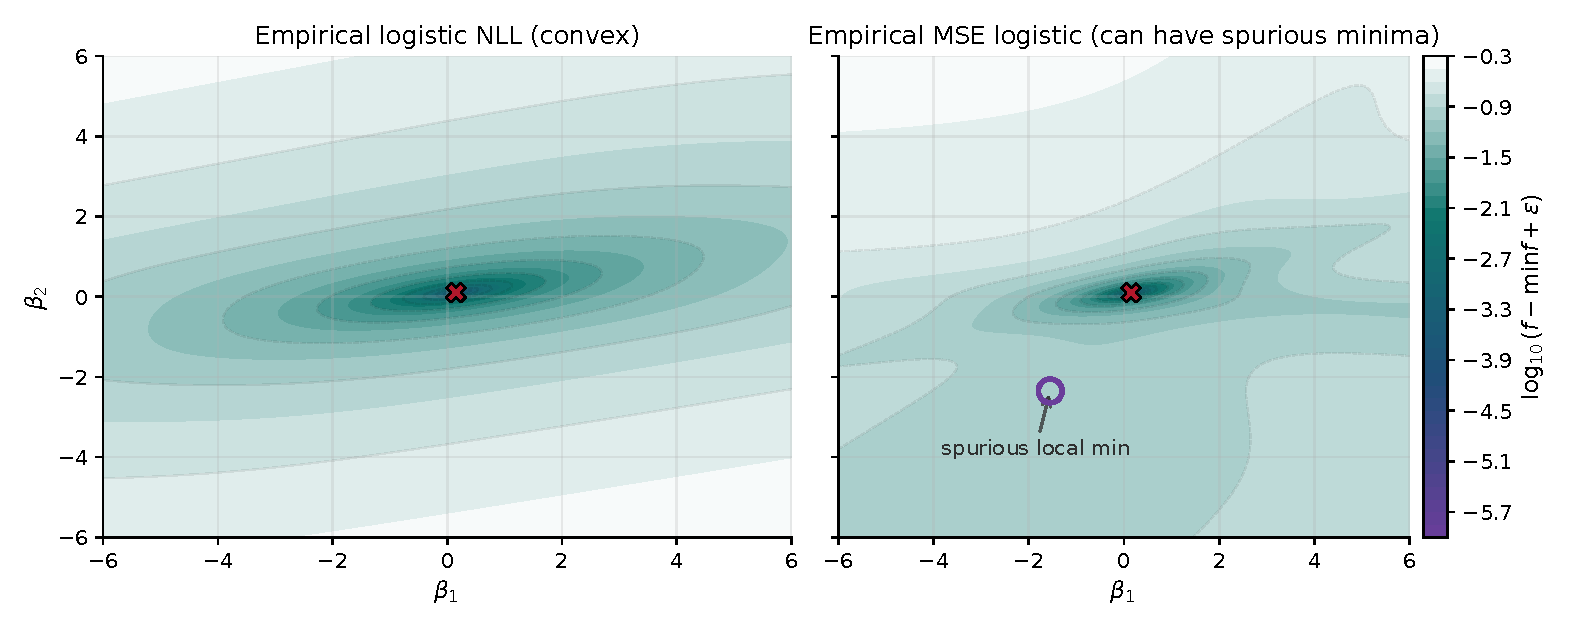
\includegraphics[width=\textwidth]{figures/handouts/convexity_optimization/fig_logistic_empirical_spurious}
  \caption{Empirical logistic landscapes on the dataset in \Cref{ex:logistic-empirical-spurious}.
  The plots show $\log_{10}(f-\min f+\varepsilon)$ for each objective.
  The red X marks the global minimizer in each panel.
  Left: the NLL is convex (one basin).
  Right: the squared-loss objective can have a spurious local minimum (circled), so a local method can get stuck.}
  \label{fig:logistic-empirical-spurious}
\end{figure}

\begin{figure}[t]
  \centering
  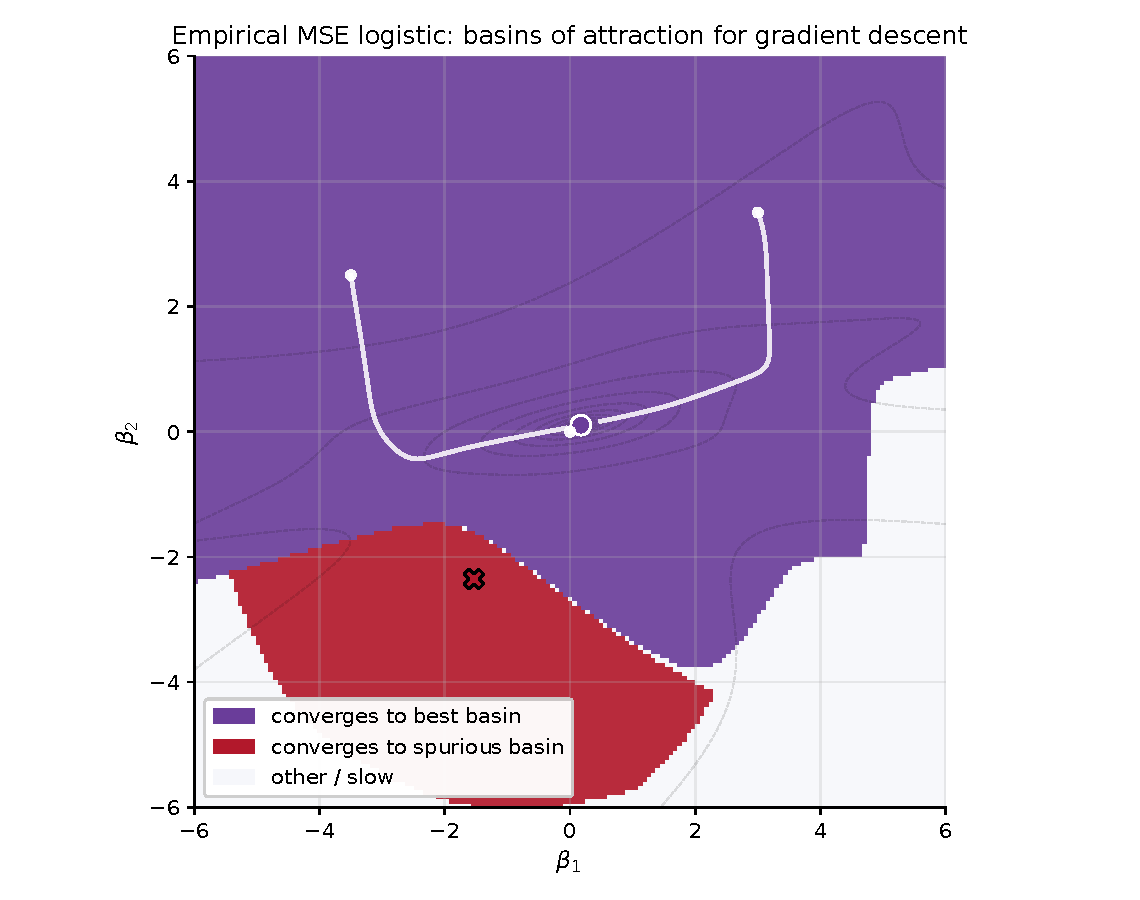
\includegraphics[width=0.92\textwidth]{figures/handouts/convexity_optimization/fig_logistic_empirical_basins}
  \caption{Basins of attraction for gradient descent on the empirical MSE-logistic objective in \Cref{ex:logistic-empirical-spurious}.
  The purple dot and red X mark the two local minimizers.
  Each initialization is colored by which local minimizer fixed-step GD (with $\eta=0.6$) converges to, and the overlaid paths show a few representative trajectories.}
  \label{fig:logistic-empirical-basins}
\end{figure}

Now assume a realizable population model:
\[
Y\mid X=x \sim \mathrm{Bernoulli}(p^\star(x)),
\qquad
p^\star(x) = \sigma(x^\top\beta^\star).
\]
Then the expected squared loss decomposes as
\[
\E\big[(Y-\sigma(X^\top\beta))^2\mid X\big]
= p^\star(X)(1-p^\star(X)) + \big(p^\star(X)-\sigma(X^\top\beta)\big)^2,
\]
so (up to an additive constant) the population objective becomes
\begin{equation}
R(\beta) = \E\big[(\sigma(X^\top\beta)-\sigma(X^\top\beta^\star))^2\big].
\label{eq:logistic-pop-risk}
\end{equation}

\begin{proposition}[One-point monotonicity in the realizable population squared-loss risk]
\label{prop:logistic-pop-one-point}
Assume $\E[\norm{X}_2]<\infty$, and let $R$ be as in \eqref{eq:logistic-pop-risk}. Then for all $\beta$,
\begin{equation}
\ip{\nabla R(\beta)}{\beta-\beta^\star} \ge 0.
\label{eq:one-point}
\end{equation}
In particular, along any ray $\beta(t)=\beta^\star+t(\beta-\beta^\star)$, the function $t\mapsto R(\beta(t))$ is nondecreasing for $t\ge 0$.
\end{proposition}

The next exercise isolates the population monotonicity calculation; structurally it plays the same role as the first-order convexity arguments in the Optimization unit.
\begin{exercise}[One-point monotonicity for realizable MSE-logistic]
\label{ex:logistic-one-point}
Prove \Cref{prop:logistic-pop-one-point}.
Let $\eta=X^\top\beta$ and $\eta^\star=X^\top\beta^\star$.
\begin{enumerate}[leftmargin=*]
  \item Differentiate under the expectation in \eqref{eq:logistic-pop-risk} to show that
  \[
  \nabla R(\beta)
  =2\,\E\Big[(\sigma(\eta)-\sigma(\eta^\star))\,\sigma'(\eta)\,X\Big].
  \]
  \item Show that
  \[
  \ip{\nabla R(\beta)}{\beta-\beta^\star}
  =2\,\E\Big[\sigma'(\eta)\,(\sigma(\eta)-\sigma(\eta^\star))(\eta-\eta^\star)\Big],
  \]
  and conclude it is nonnegative using only that $\sigma$ is increasing and $\sigma'\ge 0$.
  \item Deduce the ray-monotonicity statement by differentiating $g(t)=R(\beta^\star+t(\beta-\beta^\star))$.
\end{enumerate}
\end{exercise}

\SolutionBox[14]{%
\emph{Part (1).}
Differentiate \eqref{eq:logistic-pop-risk} under the expectation:
\[
R(\beta)=\E\big[(\sigma(X^\top\beta)-\sigma(X^\top\beta^\star))^2\big].
\]
Using the chain rule, $\nabla_\beta\sigma(X^\top\beta)=\sigma'(X^\top\beta)\,X$, hence
\[
\nabla R(\beta)
=2\,\E\Big[(\sigma(\eta)-\sigma(\eta^\star))\,\sigma'(\eta)\,X\Big],
\qquad
\eta=X^\top\beta,\ \eta^\star=X^\top\beta^\star.
\]

\emph{Part (2).}
Take the inner product with $(\beta-\beta^\star)$ and use $\ip{X}{\beta-\beta^\star}=\eta-\eta^\star$:
\[
\ip{\nabla R(\beta)}{\beta-\beta^\star}
=2\,\E\Big[\sigma'(\eta)\,(\sigma(\eta)-\sigma(\eta^\star))(\eta-\eta^\star)\Big].
\]
Since $\sigma'(\eta)\ge 0$ and $\sigma$ is increasing, we have
$(\sigma(\eta)-\sigma(\eta^\star))(\eta-\eta^\star)\ge 0$ pointwise.
Therefore the integrand is pointwise nonnegative, and the expectation is nonnegative as claimed.

\emph{Part (3) (ray monotonicity).}
For the ray $\beta(t)=\beta^\star+t(\beta-\beta^\star)$, define $g(t)=R(\beta(t))$.
By the chain rule,
\[
g'(t)=\ip{\nabla R(\beta(t))}{\beta-\beta^\star}\ge 0,
\]
so $t\mapsto R(\beta(t))$ is nondecreasing for $t\ge 0$.
(The argument uses only that the link is increasing with nonnegative derivative, so it holds for any such link function.)%
}

\begin{corollary}[Realizable population MSE-logistic has no spurious local minima]
\label{cor:logistic-pop-no-spurious}
Under the assumptions of \Cref{prop:logistic-pop-one-point}, every local minimizer of the realizable population risk $R$ in \eqref{eq:logistic-pop-risk} is global.
If in addition $\E[XX^\top]\succ 0$, then the unique global minimizer is $\beta^\star$.
\end{corollary}

\begin{exercise}[Stationarity + one-point monotonicity $\Rightarrow$ no spurious local minima]
\label{ex:logistic-one-point-no-spurious}
Prove \Cref{cor:logistic-pop-no-spurious} from \Cref{prop:logistic-pop-one-point}.
\begin{enumerate}[leftmargin=*]
  \item Let $\bar\beta$ be a local minimizer. Since $R$ is differentiable, $\nabla R(\bar\beta)=0$.
  Combine this with \Cref{eq:one-point} to show that
  \[
    0
    = \ip{\nabla R(\bar\beta)}{\bar\beta-\beta^\star}
    = 2\,\E\Big[\sigma'(\bar\eta)\,(\sigma(\bar\eta)-\sigma(\eta^\star))(\bar\eta-\eta^\star)\Big],
  \]
  where $\bar\eta=X^\top\bar\beta$ and $\eta^\star=X^\top\beta^\star$.
  Conclude that $\sigma(X^\top\bar\beta)=\sigma(X^\top\beta^\star)$ almost surely.
  \item Deduce that $R(\bar\beta)=0$, so $\bar\beta$ is a global minimizer.
  \item For uniqueness: show that if $R(\beta)=0$, then $X^\top(\beta-\beta^\star)=0$ almost surely, and deduce $\beta=\beta^\star$ under $\E[XX^\top]\succ 0$.
\end{enumerate}
\end{exercise}

\SolutionBox[14]{%
\emph{Part (1).}
Let $\bar\beta$ be a local minimizer of the differentiable function $R$.
Then $\nabla R(\bar\beta)=0$.
Applying \Cref{prop:logistic-pop-one-point} at $\beta=\bar\beta$ gives
\[
0
= \ip{\nabla R(\bar\beta)}{\bar\beta-\beta^\star}
= 2\,\E\Big[\sigma'(\bar\eta)\,(\sigma(\bar\eta)-\sigma(\eta^\star))(\bar\eta-\eta^\star)\Big],
\qquad \bar\eta=X^\top\bar\beta,\ \eta^\star=X^\top\beta^\star.
\]
The integrand is pointwise nonnegative because $\sigma'(\bar\eta)\ge 0$ and $\sigma$ is increasing, so the expectation can vanish only if the integrand is zero almost surely.
Since $\sigma'(z)>0$ for every finite $z$, this implies
\[
(\sigma(\bar\eta)-\sigma(\eta^\star))(\bar\eta-\eta^\star)=0
\qquad\text{almost surely.}
\]
Because $\sigma$ is strictly increasing, the product above is zero if and only if $\bar\eta=\eta^\star$, equivalently $\sigma(X^\top\bar\beta)=\sigma(X^\top\beta^\star)$ almost surely.

\emph{Part (2).}
If $\sigma(X^\top\bar\beta)=\sigma(X^\top\beta^\star)$ almost surely, then the integrand in \eqref{eq:logistic-pop-risk} vanishes almost surely, so
\[
R(\bar\beta)=\E\big[(\sigma(X^\top\bar\beta)-\sigma(X^\top\beta^\star))^2\big]=0.
\]
Since $R(\beta^\star)=0$ as well, $\bar\beta$ is a global minimizer.

\emph{Part (3) (uniqueness).}
If $R(\beta)=0$, then
\[
\E\big[(\sigma(X^\top\beta)-\sigma(X^\top\beta^\star))^2\big]=0,
\]
so $\sigma(X^\top\beta)=\sigma(X^\top\beta^\star)$ almost surely.
Since $\sigma$ is strictly increasing, this implies $X^\top(\beta-\beta^\star)=0$ almost surely.
Taking expectations yields
$(\beta-\beta^\star)^\top\E[XX^\top](\beta-\beta^\star)=0$.
If $\E[XX^\top]\succ 0$, then the quadratic form is strictly positive unless $\beta=\beta^\star$, so $\beta^\star$ is the unique global minimizer.%
}

The population MSE-logistic risk is nonconvex, but it still has the simple geometry that moving away from $\beta^\star$ does not help along any ray from $\beta^\star$.
This is qualitatively different from objectives like ecological logistic regression (\Cref{sec:ecological-logistic}), where aggregation introduces intrinsic nonconvexity and the landscape can have many distinct basins even under a clean population model.

Even with this benign global geometry, gradient descent can be slow because of saturation and flat plateaus.
The one-point monotonicity in \Cref{prop:logistic-pop-one-point} is a global geometry guarantee, but it is not a rate guarantee.
Far from $\beta^\star$, the squared-loss logistic objective can become very flat because the logistic link saturates:
$\sigma(z)\to 0$ or $1$ and $\sigma'(z)\to 0$ as $|z|\to\infty$.
The squared-loss gradient carries a factor of $\sigma'(X^\top\beta)$, so when the model is very confident (large $|X^\top\beta|$), the gradient can be tiny even if the objective value is not close to its minimum.
This mirrors the ``confidence weights'' story for convex NLL objectives:
in logistic NLL, curvature is largest near the decision boundary, while very confident points contribute little.
For squared loss, that same saturation suppresses the \emph{descent signal} itself, producing plateaus where $\norm{\nabla R(\beta)}_2$ is small even though $R(\beta)-R(\beta^\star)$ is not.

\begin{proposition}[Realizable squared-loss logistic: arbitrarily flat far from $\beta^\star$]
\label{prop:logistic-pop-flat}
Assume $\E[\norm{X}_2]<\infty$ and let $R$ be the realizable population risk \eqref{eq:logistic-pop-risk}.
Define $g(t)=R(t\beta^\star)$ for $t\ge 1$.
Then:
\begin{enumerate}[leftmargin=*]
  \item $g$ is nondecreasing on $[1,\infty)$ and converges to a finite limit $g(\infty)$.
  \item $\lim_{t\to\infty} g'(t)=0$ and $\lim_{t\to\infty}\norm{\nabla R(t\beta^\star)}_2=0$.
  \item If $\Pr(X^\top\beta^\star\neq 0)>0$, then $g(\infty)>0$.
\end{enumerate}
In particular, there are directions along which the landscape becomes arbitrarily flat even though the excess risk stays bounded away from $0$.
\end{proposition}

\emph{Proof idea.} See Exercise~\ref{ex:logistic-plateau}.

\begin{exercise}[Prove the plateau]
\label{ex:logistic-plateau}
In the realizable population model, let $g(t)=R(t\beta^\star)$ for $t\ge 1$.
\begin{enumerate}[leftmargin=*]
  \item Show that
  \[
    g'(t)=2\,\E\big[(\sigma(t\eta^\star)-\sigma(\eta^\star))\,\sigma'(t\eta^\star)\,\eta^\star\big],
    \qquad \eta^\star=X^\top\beta^\star,
  \]
  and conclude that $g$ is nondecreasing (hence $g(t)\to g(\infty)$ since $0\le g(t)\le 1$).
  \item Show that $g'(t)\to 0$ and $\nabla R(t\beta^\star)\to 0$ as $t\to\infty$.
  Interpret this as: \emph{without} a PL/strong-convexity-type condition, small gradient does not imply near-optimality.
  \item Assume $\Pr(\eta^\star\neq 0)>0$.
  Show that $g(\infty)>0$.
\end{enumerate}
\end{exercise}

\SolutionBox[12]{%
Write $\eta^\star=X^\top\beta^\star$ so that $g(t)=\E[(\sigma(t\eta^\star)-\sigma(\eta^\star))^2]$.

\emph{Part (1).}
Differentiate under the expectation:
by the chain rule,
\[
\frac{d}{dt}\sigma(t\eta^\star)=\sigma'(t\eta^\star)\,\eta^\star,
\]
so
\[
g'(t)
=\E\Big[2(\sigma(t\eta^\star)-\sigma(\eta^\star))\cdot \sigma'(t\eta^\star)\,\eta^\star\Big]
=2\,\E\big[(\sigma(t\eta^\star)-\sigma(\eta^\star))\,\sigma'(t\eta^\star)\,\eta^\star\big].
\]
For $t\ge 1$, $\sigma(t\eta^\star)-\sigma(\eta^\star)$ has the same sign as $(t-1)\eta^\star$ since $\sigma$ is increasing.
Because $\sigma'\ge 0$, the integrand is pointwise nonnegative, hence $g'(t)\ge 0$ and $g$ is nondecreasing.
Since $g(t)\in[0,1]$, it follows that $g(t)\to g(\infty)$ for some finite limit $g(\infty)$.

\emph{Part (2).}
For each fixed $\eta^\star\neq 0$, we have $t\eta^\star\to \pm\infty$ and therefore $\sigma'(t\eta^\star)\to 0$ as $t\to\infty$.
Also,
\[
\big|(\sigma(t\eta^\star)-\sigma(\eta^\star))\,\sigma'(t\eta^\star)\,\eta^\star\big|
\le \sigma'(0)\,|\eta^\star|
\le \sigma'(0)\,\norm{\beta^\star}_2\,\norm{X}_2,
\]
which is integrable since $\E[\norm{X}_2]<\infty$.
We will use the following standard fact: if random variables $Z_t$ satisfy $|Z_t|\le W$ with $\E[W]<\infty$ and $Z_t\to 0$ almost surely, then $\E[Z_t]\to 0$.
Applying this fact here gives $g'(t)\to 0$ as $t\to\infty$.

\smallskip
Similarly, differentiating \eqref{eq:logistic-pop-risk} gives
\[
\nabla R(t\beta^\star)
=2\,\E\big[(\sigma(t\eta^\star)-\sigma(\eta^\star))\,\sigma'(t\eta^\star)\,X\big].
\]
The integrand norm is bounded by $2\sigma'(0)\norm{X}_2$, and for each fixed $X$ the factor $\sigma'(t\eta^\star)$ tends to $0$ (or the bracketed term vanishes when $\eta^\star=0$), so the same reasoning lets us pass the limit through the expectation and conclude $\nabla R(t\beta^\star)\to 0$.

\emph{Part (3).}
As $t\to\infty$ we have $\sigma(t\eta^\star)\to 1$ when $\eta^\star>0$, $\sigma(t\eta^\star)\to 0$ when $\eta^\star<0$, and $\sigma(t\eta^\star)=\sigma(\eta^\star)=1/2$ when $\eta^\star=0$.
Since $0\le (\sigma(t\eta^\star)-\sigma(\eta^\star))^2\le 1$, we can apply the same fact (with $W=1$) to pass the limit through the expectation and obtain
\[
g(\infty)=\E\Big[(1-\sigma(\eta^\star))^2\mathbf{1}\{\eta^\star>0\} + \sigma(\eta^\star)^2\mathbf{1}\{\eta^\star<0\}\Big].
\]
If $\Pr(\eta^\star\neq 0)>0$, then the integrand is strictly positive on $\{\eta^\star\neq 0\}$, so $g(\infty)>0$.

Along this ray, the risk can remain bounded away from $0$ while the gradient (and directional derivative) goes to $0$.
Without a condition like PL/strong convexity, a small gradient does not by itself certify near-optimality.
}

Conditions like strong convexity or the PL inequality (\Cref{def:pl-inequality}) prevent this phenomenon: they rule out large flat regions away from the optimum by relating gradient size to suboptimality.
\Cref{prop:logistic-pop-flat} shows the realizable squared-loss logistic risk does not have such a global guarantee in general.

In the realizable population model, the one-point monotonicity in \Cref{prop:logistic-pop-one-point} is a \emph{global} geometric statement.
To get an actual rate for gradient descent, we also need a \emph{local curvature} condition near $\beta^\star$.
One simple sufficient condition is bounded features, which implies local strong convexity (hence a linear rate) around the optimum.

\begin{proposition}[Local linear convergence of gradient descent near $\beta^\star$]
\label{prop:logistic-pop-local-rate}
Assume $\E[XX^\top]\succeq \lambda I_d$ and $\norm{X}_2\le R$ almost surely for some $\lambda,R>0$.
Then at $\beta^\star$,
\[
\Hess R(\beta^\star)\succeq m_0 I_d,
\qquad
m_0 = 2\,\sigma'(R\norm{\beta^\star}_2)^2\,\lambda,
\]
and there exist $r>0$ and constants $0<m\le L<\infty$ such that the population risk $R$ in \eqref{eq:logistic-pop-risk} is $m$-strongly convex and $L$-smooth on the ball $\{\beta:\ \norm{\beta-\beta^\star}_2\le r\}$.
Consequently, gradient descent with step size $1/L$ initialized in this ball satisfies
\[
R(\beta^{(k)})-R(\beta^\star)
\le \left(1-\frac{m}{L}\right)^k\bigl(R(\beta^{(0)})-R(\beta^\star)\bigr)
\qquad\text{(see \citealp[\S9.3]{boyd_vandenberghe_2004_convex}).}
\]
\end{proposition}

\begin{proof}
Differentiate \eqref{eq:logistic-pop-risk} twice.
At $\beta=\beta^\star$, the cross term vanishes and the Hessian simplifies to
\[
\Hess R(\beta^\star)=2\,\E\big[\sigma'(X^\top\beta^\star)^2\,XX^\top\big].
\]
Since $\norm{X^\top\beta^\star}\le \norm{X}_2\norm{\beta^\star}_2\le R\norm{\beta^\star}_2$ almost surely, we have
$\sigma'(X^\top\beta^\star)\ge \sigma'(R\norm{\beta^\star}_2)>0$ almost surely (since $\sigma'$ is even and decreases with $|z|$), hence
\[
\Hess R(\beta^\star)\succeq 2\,\sigma'(R\norm{\beta^\star}_2)^2\,\E[XX^\top]\succeq 2\,\sigma'(R\norm{\beta^\star}_2)^2\,\lambda I_d.
\]
This is the claimed bound with $m_0=2\,\sigma'(R\norm{\beta^\star}_2)^2\,\lambda$.
Because $R$ is twice continuously differentiable and $\norm{X}_2\le R$ almost surely, $\Hess R(\beta)$ varies continuously in $\beta$ and is bounded on compact sets.
Therefore, on a sufficiently small ball around $\beta^\star$, the Hessian is bounded below by (say) $\tfrac12 m_0 I_d$ and above by $L I_d$ for some finite $L$, which gives local strong convexity and smoothness.
The linear convergence rate for gradient descent on an $m$-strongly convex and $L$-smooth function is standard (cited above).
\end{proof}

Under misspecification, hard multimodality can return.
If $p^\star(x)$ is not representable as $\sigma(x^\top\beta)$ (e.g.\ marginalizing over latent classes can yield mixtures of logits), then \eqref{eq:one-point} need not hold, and the population squared-loss risk can become bimodal with spurious local minima.
Benign global geometry often hinges on model and data assumptions.
This is one reason MLE (convex NLL) is often more stable than squared-loss fitting in logistic-type binary regression models.

\begin{example}[Misspecification can create a spurious local minimum for squared-loss logistic regression]
\label{ex:logistic-misspecified-spurious}
Consider a 1D feature $X$ that takes values $\{-2,-1,1,2\}$ with equal probability, and parameterize $\beta=(\beta_0,\beta_1)$ so that $q_\beta(x)=\sigma(\beta_0+\beta_1 x)$.
Let the true conditional probabilities be
\[
p^\star(-2)=0.49,\quad p^\star(-1)=0.87,\quad p^\star(1)=0.92,\quad p^\star(2)=0.36.
\]
This $p^\star$ is not representable as $q_\beta$, since it is not monotone in $x$.

For the population squared-loss risk $R_{\mathrm{MSE}}(\beta)=\E[(q_\beta(X)-p^\star(X))^2]$, a direct evaluation shows two distinct basins:
numerically, evaluating $R_{\mathrm{MSE}}$ on a grid reveals a global minimizer and a spurious local minimizer.
See \Cref{fig:logistic-landscape-2d}.
\end{example}

\begin{figure}[t]
  \centering
  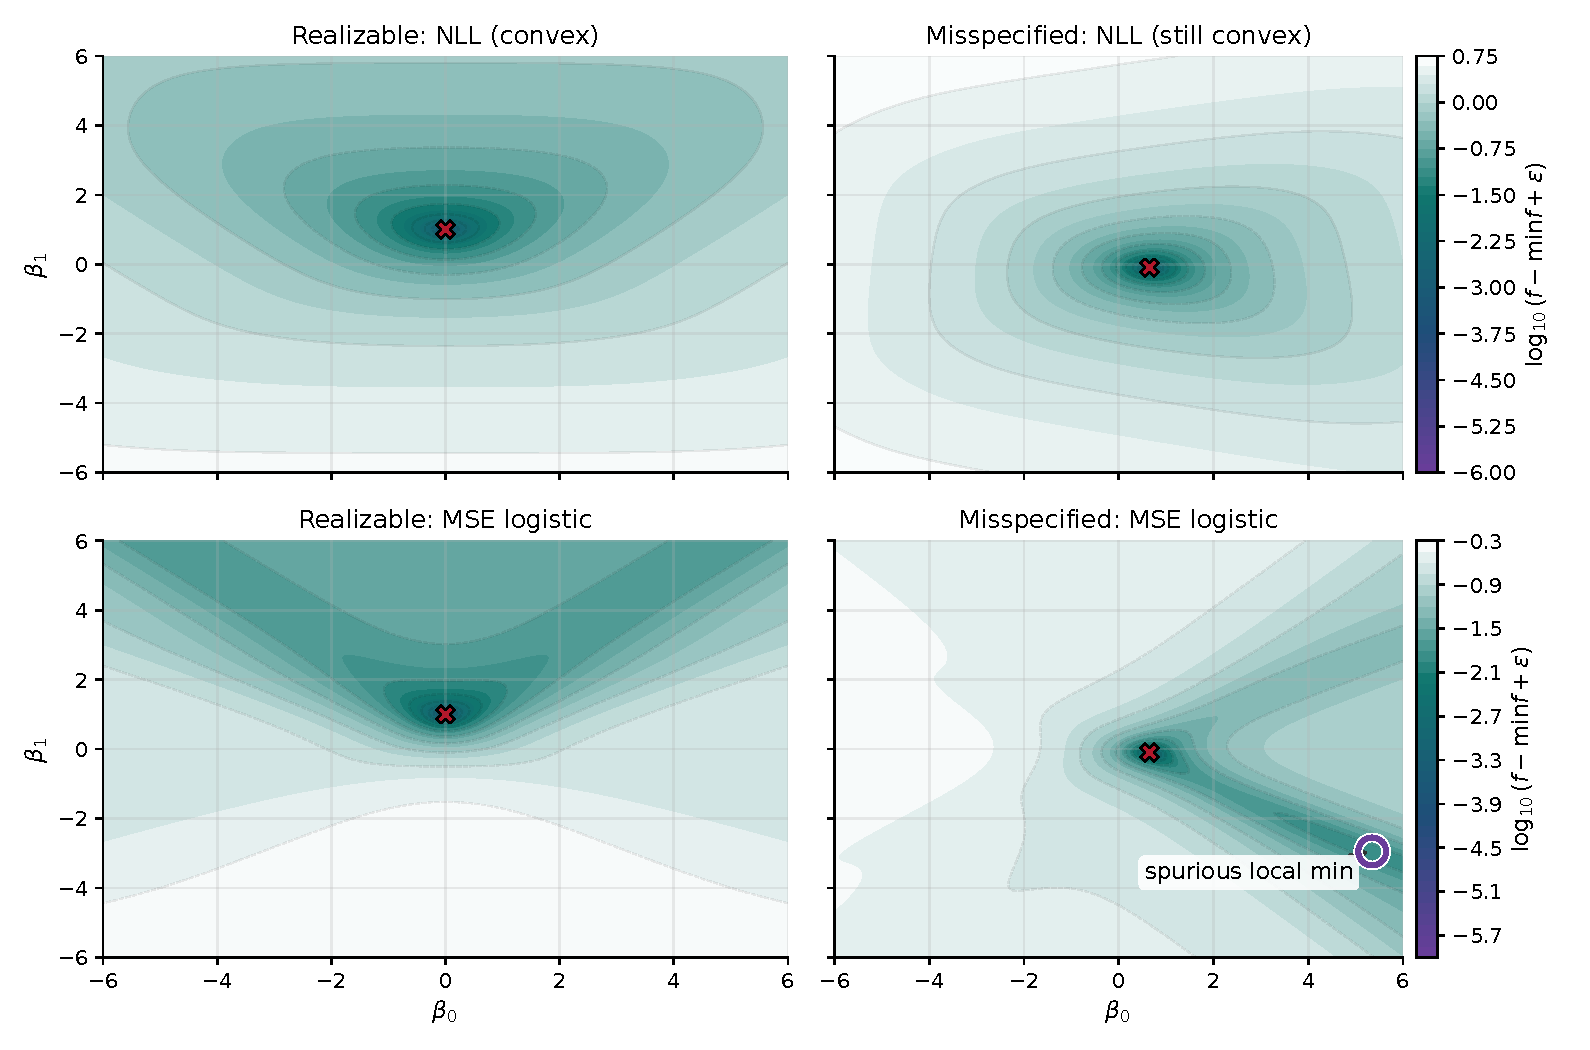
\includegraphics[width=\textwidth]{figures/handouts/convexity_optimization/fig_logistic_landscape_2d}
  \caption{A consistent contourf view of logistic landscapes in a 2D parameterization $\beta=(\beta_0,\beta_1)$.
  The plots show $\log_{10}(f-\min f+\varepsilon)$ for each objective, which makes basins comparable across panels.
  The red X marker indicates the global minimizer in each panel; in the bottom-right plot, the circled point is a spurious local minimum.
  In this example, the NLL landscape is unimodal in both realizable and misspecified settings, while the squared-loss landscape can develop extra basins under misspecification.}
  \label{fig:logistic-landscape-2d}
\end{figure}

% ------------------------------------------------------------
Example~I separates three distinct regimes.
Empirical MSE-logistic can create spurious basins; the realizable population risk has no spurious local minima but can still be slow because of broad plateaus; and misspecification can bring back genuinely wrong stable basins.
The response depends on the regime: use a stable objective when possible, use damping or line search when curvature is unreliable, and use restarts or stronger initializations when multiple basins are present.

% ------------------------------------------------------------
\section[Example II (phase retrieval)]{Example II: multimodality from symmetry, but only global optima in phase retrieval}
\label{sec:phase-retrieval}

In coherent diffraction imaging, optics, and astronomy, sensors measure intensities and lose phase.
A canonical real model is \emph{phase retrieval}:
\[
y_i = (a_i^\top x^\star)^2,\qquad i=1,\dots,m,
\]
where $x^\star\in\R^d$ is the unknown signal and $a_i$ are known sensing vectors.
A standard nonconvex least-squares objective is
\begin{equation}
F(x)=\frac{1}{4m}\sum_{i=1}^m\big((a_i^\top x)^2 - y_i\big)^2.
\label{eq:phase-empirical}
\end{equation}
This objective is nonconvex for structural reasons (it involves squares of linear forms),
and it is \emph{inherently} multimodal because $x^\star$ and $-x^\star$ generate the same data.

Like squared-loss logistic regression, phase retrieval is a smooth, nonconvex least-squares objective.
But here the nonconvexity is driven primarily by a \emph{symmetry}: $x^\star$ and $-x^\star$ generate the same data.
In population (for Gaussian designs), this symmetry produces multiple global optima but \emph{no} suboptimal local minima; the remaining stationary points are saddles.
This is ``benign'' nonconvexity (a strict-saddle picture), and it contrasts with ecological logistic regression (\Cref{sec:ecological-logistic}), where aggregation creates intrinsic nonconvexity and can lead to many distinct basins.
This ``benign geometry'' picture (multiple equivalent global minimizers; strict saddles elsewhere) appears broadly in modern tractable nonconvex problems; see \citet[\S2]{sun_qu_wright_2015_nonconvex_not_scary} and \citet[\S1]{zhang_qu_wright_2020_symmetry_geometry}.

\begin{figure}[t]
  \centering
  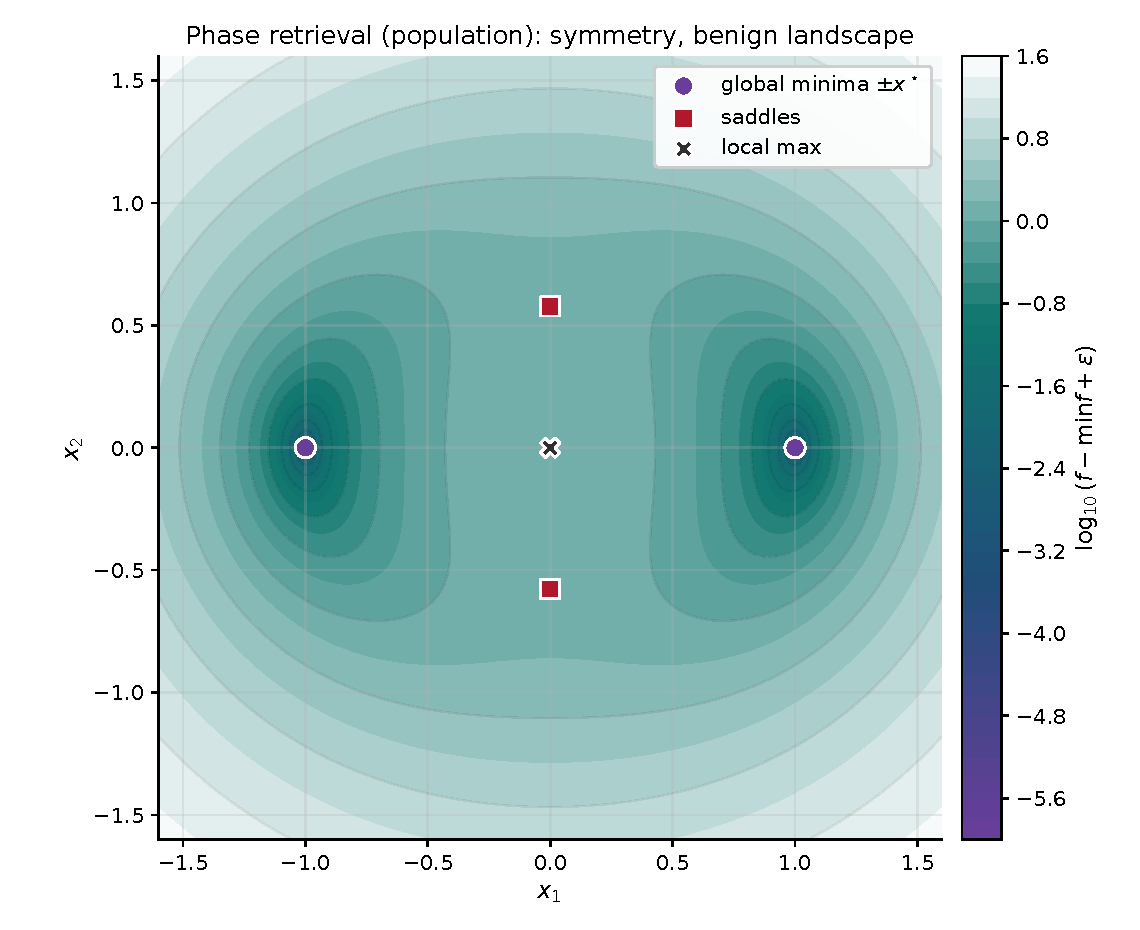
\includegraphics[width=0.86\textwidth]{figures/handouts/convexity_optimization/fig_phase_retrieval_landscape}
  \caption{Population phase retrieval in $d=2$: the landscape is nonconvex and symmetric ($x\sim -x$), but the only local minima are the two global minima $\pm x^\star$; other critical points are saddles or a local maximum at the origin.}
  \label{fig:phase-retrieval-landscape}
\end{figure}

For a clean population model, assume $a\sim N(0,I_d)$ and consider the \emph{population} objective
\begin{equation}
  f(x)=\frac12\,\E\Big[\big((a^\top x)^2 - (a^\top x^\star)^2\big)^2\Big].
  \label{eq:phase-pop}
\end{equation}

\begin{proposition}[Population phase retrieval: nonconvex but no spurious local minima]
\label{prop:phase-retrieval-benign}
For $f$ in \eqref{eq:phase-pop},
\begin{equation}
  f(x)
  =\frac{3}{2}\norm{x}^4 - \norm{x}^2\norm{x^\star}^2 - 2\ip{x}{x^\star}^2 + \frac{3}{2}\norm{x^\star}^4,
  \label{eq:phase-pop-closed-form}
\end{equation}
and the stationary points are:
\begin{enumerate}[leftmargin=*]
  \item global minima $x=\pm x^\star$ (value $0$),
  \item a local maximum at $x=0$,
  \item a saddle set $\{x:\ x\perp x^\star,\ \norm{x}=\norm{x^\star}/\sqrt{3}\}$.
\end{enumerate}
In particular, every local minimum is global.
\end{proposition}

\begin{exercise}[Phase retrieval: derive and classify the population stationary points]
\label{ex:phase-pop-derivation}
Prove \Cref{prop:phase-retrieval-benign}.
\begin{enumerate}[leftmargin=*]
  \item Expand \eqref{eq:phase-pop} and use the Gaussian fourth-moment identities
  \[
  \E[(a^\top u)^4]=3\norm{u}^4,
  \qquad
  \E[(a^\top u)^2(a^\top v)^2]=\norm{u}^2\norm{v}^2 + 2\ip{u}{v}^2,
  \]
  to obtain \eqref{eq:phase-pop-closed-form}.
  \item Differentiate \eqref{eq:phase-pop-closed-form} to get an explicit formula for $\nabla f(x)$.
  \item Solve $\nabla f(x)=0$ by decomposing $x=\alpha x^\star + u$ with $u\perp x^\star$.
  \item Classify the stationary points as global minima, a local maximum, and a saddle set.
\end{enumerate}
\end{exercise}

\SolutionBox[22]{%
\emph{Part (1) (closed form).}
Expanding the square in \eqref{eq:phase-pop} gives
\[
f(x)
=\frac12\,\E\big[(a^\top x)^4\big]
\;-\;\E\big[(a^\top x)^2(a^\top x^\star)^2\big]
\;+\;\frac12\,\E\big[(a^\top x^\star)^4\big].
\]
Apply the stated Gaussian fourth-moment identities with $u=x$ and $v=x^\star$ to get
\[
\E[(a^\top x)^4]=3\norm{x}^4,\qquad
\E[(a^\top x^\star)^4]=3\norm{x^\star}^4,
\]
and
\[
\E[(a^\top x)^2(a^\top x^\star)^2]=\norm{x}^2\norm{x^\star}^2 + 2\ip{x}{x^\star}^2.
\]
Substituting yields \eqref{eq:phase-pop-closed-form}.

\emph{Part (2) (gradient).}
Differentiate \eqref{eq:phase-pop-closed-form}:
\[
\nabla f(x)
= 6\norm{x}^2 x - 2\norm{x^\star}^2 x - 4\ip{x}{x^\star}x^\star
= (6\norm{x}^2-2\norm{x^\star}^2)x - 4\ip{x}{x^\star}x^\star.
\]

\emph{Part (3) (stationary points).}
Let $r=\norm{x^\star}_2$ and decompose $x=\alpha x^\star + u$ with $u\perp x^\star$.
Then $\ip{x}{x^\star}=\alpha r^2$ and $\norm{x}^2=\alpha^2r^2+\norm{u}^2$.
Setting $\nabla f(x)=0$ and matching the $u$ and $x^\star$ components gives
\[
(6\norm{x}^2-2r^2)\,u=0,
\qquad
\alpha\,(6\norm{x}^2-6r^2)=0.
\]
If $u=0$, then either $\alpha=0$ (so $x=0$) or $\norm{x}^2=r^2$ (so $\alpha=\pm 1$ and $x=\pm x^\star$).
If $u\neq 0$, then the first equation forces $\norm{x}^2=r^2/3$, and the second forces $\alpha=0$, hence
$x\perp x^\star$ and $\norm{x}=r/\sqrt{3}$.
This gives exactly the stationary-point list in \Cref{prop:phase-retrieval-benign}.

\emph{Part (4) (classification).}
Since $f$ in \eqref{eq:phase-pop} is an expectation of a square, $f(x)\ge 0$ for all $x$.
Also $f(\pm x^\star)=0$, so $\pm x^\star$ are global minima.

For $x=0$, the expansion \eqref{eq:phase-pop-closed-form} shows
\[
f(0)-f(x)= r^2\norm{x}^2 + 2\ip{x}{x^\star}^2 - \frac{3}{2}\norm{x}^4,
\]
which is strictly positive for all sufficiently small $x\neq 0$ (the quadratic term dominates), so $x=0$ is a local maximum.

Finally, if $x\perp x^\star$ and $\norm{x}=r/\sqrt{3}$, then the univariate restriction $t\mapsto f(x+t x^\star)$ has negative second derivative at $t=0$, so there is a direction of negative curvature.
Hence these points are saddles, and every local minimum is global.%
}

This is symmetry-driven nonconvexity with a strict-saddle geometry:
every non-optimal stationary point has a direction of negative curvature.

Phase retrieval is typically approached via the two-stage template in \Cref{alg:two-stage-template}:
use a cheap global initializer, then run a local method.
In the Gaussian model, there is a clean way to build a provably good direction estimate from a simple moment identity.
Assume the noiseless Gaussian design model $a_i \stackrel{\mathrm{iid}}{\sim} N(0,I_d)$ with measurements $y_i=(a_i^\top x^\star)^2$.
Define the \emph{spectral matrix}
\[
  Y = \frac{1}{m}\sum_{i=1}^m y_i a_i a_i^\top.
\]
Also define the radius estimate
\[
  \hat r^2 = \frac{1}{m}\sum_{i=1}^m y_i,
\]
which satisfies $\E[\hat r^2]=\norm{x^\star}_2^2$.
If $\hat u$ is a unit-norm top eigenvector of $Y$, then the standard spectral initializer is $x^{(0)}=\hat r\,\hat u$.

The next proposition explains why this initialization is reasonable.
It shows that (i) the population matrix $\E[Y]$ has a unique leading eigenvector in the $x^\star$ direction, and (ii) if the empirical $Y$ is close to $\E[Y]$ in operator norm then its leading eigenvector must be close to $\pm x^\star/\norm{x^\star}_2$.
(Here $\norm{M}_{\mathrm{op}}$ denotes the operator norm, i.e.\ the largest absolute eigenvalue for a symmetric matrix $M$.)

\begin{proposition}[Gaussian phase retrieval: why the spectral initializer points at $x^\star$]
\label{prop:phase-spectral-init}
Assume $x^\star\neq 0$, let $a\sim N(0,I_d)$, and set $y=(a^\top x^\star)^2$.
Write $r=\norm{x^\star}_2$ and $u^\star=x^\star/r$.
Define the population matrix
\[
  Y_{\mathrm{pop}} = \E\big[y\,a a^\top\big]
  = \E\big[(a^\top x^\star)^2 a a^\top\big].
\]
Then
\[
  Y_{\mathrm{pop}}=r^2 I_d + 2x^\star(x^\star)^\top,
\]
so the unique leading eigenvector of $Y_{\mathrm{pop}}$ is $u^\star$.
Moreover, if $Y$ is any symmetric matrix satisfying
\[
\norm{Y-Y_{\mathrm{pop}}}_{\mathrm{op}} \le \varepsilon\, r^2
\qquad\text{for some }\varepsilon\in(0,1),
\]
then for every unit-norm leading eigenvector $\hat u$ of $Y$ there exists a sign $s\in\{\pm 1\}$ such that
$\norm{\hat u-su^\star}_2\le \sqrt{2\varepsilon}$.
\end{proposition}

\begin{exercise}[Phase retrieval: why spectral initialization points at $x^\star$]
\label{ex:phase-spectral-spike}
Prove \Cref{prop:phase-spectral-init}.
Conclude that if the empirical matrix $Y$ is close to $Y_{\mathrm{pop}}$ in operator norm, then its top eigenvector is close to $\pm u^\star$ and the spectral initializer $x^{(0)}=\hat r\,\hat u$ is close to $\pm x^\star$.
\emph{Hint:} to compute $Y_{\mathrm{pop}}$, you can either compute entries using the Gaussian fourth-moment identity
$\E[a_i a_j a_k a_\ell]=\delta_{ij}\delta_{k\ell}+\delta_{ik}\delta_{j\ell}+\delta_{i\ell}\delta_{jk}$,
or compute the entries directly by expanding.
For the perturbation bound, compare quadratic forms $v^\top Y v$ and use $|v^\top (Y-Y_{\mathrm{pop}}) v|\le \norm{Y-Y_{\mathrm{pop}}}_{\mathrm{op}}$ for unit $v$.
Finally, explain in a sentence why one expects $\norm{Y-Y_{\mathrm{pop}}}_{\mathrm{op}}$ to be small when $m$ is large in the Gaussian model.
\end{exercise}

\SolutionBox[20]{%
Write $u=x^\star$ and expand $y=(a^\top u)^2=\sum_{k,\ell} u_k u_\ell a_k a_\ell$.
For each entry $(i,j)$,
\[
\E\!\big[y\,a_i a_j\big]
=\sum_{k,\ell} u_k u_\ell\,\E[a_i a_j a_k a_\ell]
=\sum_{k,\ell} u_k u_\ell\bigl(\delta_{ij}\delta_{k\ell}+\delta_{ik}\delta_{j\ell}+\delta_{i\ell}\delta_{jk}\bigr).
\]
The first term gives $\delta_{ij}\sum_k u_k^2=\delta_{ij}\norm{u}_2^2$.
The second and third terms each give $u_i u_j$.
Thus $\E[y\,a_i a_j]=\norm{u}_2^2\,\delta_{ij}+2u_i u_j$, i.e.
$Y_{\mathrm{pop}}=\norm{u}_2^2 I_d + 2uu^\top$.

For eigenvalues, note that $Y_{\mathrm{pop}}u=(\norm{u}_2^2+2\norm{u}_2^2)u=3\norm{u}_2^2 u$.
If $w\perp u$, then $uu^\top w=0$ so $Y_{\mathrm{pop}}w=\norm{u}_2^2 w$.
Hence the unique top eigenspace is $\mathrm{span}\{u\}$.

Let $r=\norm{u}_2$ and $u^\star=u/r$.
Let $\hat u$ be a unit top eigenvector of $Y$.
Write $E=Y-Y_{\mathrm{pop}}$ and assume $\norm{E}_{\mathrm{op}}\le \varepsilon r^2$.
Then
\[
\hat u^\top Y_{\mathrm{pop}} \hat u
= \hat u^\top Y \hat u - \hat u^\top E \hat u
\ge \lambda_{\max}(Y) - \norm{E}_{\mathrm{op}}
\ge (u^\star)^\top Y u^\star - \norm{E}_{\mathrm{op}}
\ge 3r^2 - 2\varepsilon r^2.
\]
On the other hand,
$
\hat u^\top Y_{\mathrm{pop}} \hat u
= r^2 + 2r^2\,|\ip{\hat u}{u^\star}|^2.
$
Combining gives $|\ip{\hat u}{u^\star}|^2\ge 1-\varepsilon$.
Choosing the sign that maximizes the inner product,
\[
\min\{\norm{\hat u-u^\star}_2,\norm{\hat u+u^\star}_2\}^2
=2\bigl(1-|\ip{\hat u}{u^\star}|\bigr)
\le 2\bigl(1-|\ip{\hat u}{u^\star}|^2\bigr)
\le 2\varepsilon.
\]

The matrix $Y$ is an empirical average of i.i.d.\ symmetric matrices with mean $Y_{\mathrm{pop}}$.
To make this quantitative in high dimensions, one uses concentration inequalities for random matrices to bound $\norm{Y-Y_{\mathrm{pop}}}_{\mathrm{op}}$ with high probability; see \citet[\S2.2]{zhang_qu_wright_2020_symmetry_geometry} for discussion and references.
These probability tools are largely orthogonal to our focus here.%
}

Once you have an initialization that is close to $\pm x^\star$, the local stage behaves like the convex story again.
In the Gaussian population objective, $\pm x^\star$ are not only global minima: they are \emph{locally strongly convex} minima, so the standard local strong-convexity analysis from the Optimization unit gives a linear rate while the iterates remain in that neighborhood.

\begin{exercise}[Phase retrieval: local convexity near $\pm x^\star$ in the population objective]
\label{ex:phase-pop-local-strong-convex}
For the population objective $f$ in \eqref{eq:phase-pop-closed-form}, compute the Hessian $\Hess f(x)$ and show that
\[
\Hess f(x^\star)=4\norm{x^\star}_2^2 I_d + 8x^\star(x^\star)^\top.
\]
Deduce the eigenvalues of $\Hess f(x^\star)$ and interpret this as a local condition-number statement near $x^\star$.
\end{exercise}

\SolutionBox[12]{%
Differentiate the gradient formula in the solution to \Cref{ex:phase-pop-derivation}:
for $x\in\R^d$,
\[
\Hess f(x)=12xx^\top + (6\norm{x}_2^2-2\norm{x^\star}_2^2)I_d - 4x^\star(x^\star)^\top.
\]
At $x=x^\star$ this becomes
\[
\Hess f(x^\star)=(12-4)x^\star(x^\star)^\top + 4\norm{x^\star}_2^2 I_d
=8x^\star(x^\star)^\top + 4\norm{x^\star}_2^2 I_d.
\]
Along $u^\star=x^\star/\norm{x^\star}_2$ the eigenvalue is $12\norm{x^\star}_2^2$, and along any direction orthogonal to $x^\star$ the eigenvalue is $4\norm{x^\star}_2^2$.
So near $x^\star$ the population objective is well conditioned (local condition number $3$), which is exactly the regime where local methods behave like in the convex case.%
}

These pieces give the standard Gaussian-model story:
spectral initialization supplies a direction close to $\pm x^\star$, and the local geometry near $\pm x^\star$ is strongly convex, so local methods converge quickly once initialized there.
Rigorous finite-sample analyses follow this template; see \citet[\S2.2]{zhang_qu_wright_2020_symmetry_geometry} and references therein.

Phase retrieval shows a different kind of nonconvexity.
The sign symmetry creates multiple optima, but they are equivalent, and the remaining stationary points are saddles rather than bad local minima.
The right response is therefore not exhaustive global search; it is a coarse initializer, such as a spectral method, followed by local refinement inside the basin of $\pm x^\star$.



% ------------------------------------------------------------
\section[Example III (ecological logistic)]{Example III: hard nonconvexity from aggregation in ecological logistic regression}
\label{sec:ecological-logistic}

In some applications we observe covariates at the unit level but only aggregated outcomes.
For example, we might see covariates $x_{g,1},\dots,x_{g,n_g}$ for individuals in a group (a precinct, a cohort, a batch),
but instead of observing the binary outcomes $Y_{g,i}\in\{0,1\}$ we only observe the group total
\[
Z_g = \sum_{i=1}^{n_g} Y_{g,i}.
\]
Many different binary vectors $(Y_{g,1},\dots,Y_{g,n_g})$ can produce the same total $Z_g$, so the likelihood for $\beta$ must marginalize over a large discrete set of latent ``assignments.''

Assume a logistic model at the unit level:
\[
\Pr(Y_{g,i}=1\mid x_{g,i},\beta)=\sigma(x_{g,i}^\top\beta),
\qquad i=1,\dots,n_g,
\]
with conditional independence across $i$ given the covariates.
Write $p_{g,i}(\beta)=\sigma(x_{g,i}^\top\beta)$.
Then $Z_g$ is a sum of independent but non-identically distributed Bernoulli random variables (a Poisson--binomial model), and the marginal likelihood contains $\binom{n_g}{z_g}$ terms.
The resulting negative log-likelihood is typically nonconvex in $\beta$.
This combinatorial marginalization also creates a separate difficulty that is easy to miss if we focus only on the geometry:
when $n_g$ is large, the likelihood term $\Pr(Z_g=z_g\mid x_{g,1},\dots,x_{g,n_g},\beta)$ can be expensive to evaluate repeatedly inside an optimizer.
The naive computation is literally a sum over $\binom{n_g}{z_g}$ assignments (as in \Cref{ex:eco-logistic-nonconvex}), which is intractable for large groups.
This ``optimization + marginalization'' pattern is common in latent-variable models: hard landscapes and expensive objective evaluations can come together.

An empirical negative log-likelihood objective for $G$ independent groups is
\begin{equation}
  f(\beta)
  =
  -\frac{1}{G}\sum_{g=1}^G \log \Pr(Z_g=z_g \mid x_{g,1},\dots,x_{g,n_g},\beta).
  \label{eq:eco-logistic-obj}
\end{equation}
Two edge cases are instructive.
In the special case where the covariates are constant within each group ($x_{g,i}\equiv x_g$), we have
$Z_g\sim \mathrm{Binomial}(n_g,\sigma(x_g^\top\beta))$, and \eqref{eq:eco-logistic-obj} reduces to the usual convex binomial logistic-regression objective from the Optimization unit.
At the other extreme, if $d=1$ with $\beta=(\beta_0,\beta_1)$ and each group contains covariates in $\pm$ pairs (for every $x$ the value $-x$ appears with the same multiplicity), then the marginal likelihood is symmetric in the slope: it is unchanged under $\beta_1\mapsto -\beta_1$.
This kind of symmetry reflects a genuine non-identifiability from totals alone.

\begin{exercise}[Ecological logistic regression: two easy special cases]
\label{ex:eco-logistic-edge-cases}
\begin{enumerate}[leftmargin=*]
  \item Suppose $x_{g,i}\equiv x_g$ within each group.
  Show that $Z_g\sim \mathrm{Binomial}(n_g,\sigma(x_g^\top\beta))$ and conclude that the corresponding negative log-likelihood is convex in $\beta$.
  \item Assume $d=1$ with $\beta=(\beta_0,\beta_1)$ and suppose the multiset $\{x_1,\dots,x_n\}$ is symmetric: for every $x$ it contains $-x$ with the same multiplicity.
  Show that, for every $z$,
  \[
    \Pr(Z=z\mid x_1,\dots,x_n,(\beta_0,\beta_1))
    =
    \Pr(Z=z\mid x_1,\dots,x_n,(\beta_0,-\beta_1)).
  \]
  Conclude that the likelihood for $\beta_1$ is an even function, so the sign of the slope is not identifiable from $Z$ alone in such a balanced design.
\end{enumerate}
\end{exercise}

\SolutionBox[14]{%
\emph{Part (1).}
If $x_{g,i}\equiv x_g$, then conditional on $x_g$ the unit-level outcomes are i.i.d.\ Bernoulli with success probability $\sigma(x_g^\top\beta)$.
Therefore $Z_g=\sum_{i=1}^{n_g}Y_{g,i}\sim \mathrm{Binomial}(n_g,\sigma(x_g^\top\beta))$.
Up to an additive constant (independent of $\beta$), the per-group negative log-likelihood can be written as a function of the scalar $\eta=x_g^\top\beta$:
\[
\ell_g(\beta)
= -z_g\,\eta + n_g\log(1+e^\eta).
\]
Since $\frac{d^2}{d\eta^2}\ell_g(\eta)=n_g\,\sigma'(\eta)\ge 0$, the map $\eta\mapsto \ell_g(\eta)$ is convex.
Composing a convex function with a linear map $\beta\mapsto x_g^\top\beta$ preserves convexity, so $\ell_g$ is convex in $\beta$.
Summing over $g$ preserves convexity, hence the full objective is convex.

\emph{Part (2).}
Write $p_i(\beta_0,\beta_1)=\sigma(\beta_0+\beta_1 x_i)$.
Replacing $\beta_1$ by $-\beta_1$ replaces $p_i$ by $\tilde p_i=\sigma(\beta_0-\beta_1 x_i)$.
By the assumed symmetry of the multiset $\{x_i\}$, the multiset $\{\tilde p_i\}$ is the same as $\{p_i\}$ up to a permutation (each $x$ is paired with $-x$).
But the distribution of $Z=\sum_i Y_i$ depends only on the multiset of success probabilities, not on how they are ordered, so $\Pr(Z=z\mid x_1,\dots,x_n,(\beta_0,\beta_1))=\Pr(Z=z\mid x_1,\dots,x_n,(\beta_0,-\beta_1))$ for every $z$.
Thus the likelihood is an even function of $\beta_1$, which means the sign of the slope is not identifiable from totals in this balanced design.%
}

This example ties directly to the empirical-versus-population theme from Example~I.
There the bad basins can be a finite-sample artifact under benign population geometry; here the nonconvexity is intrinsic, because even under the correct model and infinite data aggregation forces us to marginalize over discrete latent assignments.
That marginalization step is also the bridge to the Expectation--maximization subsection of the Augmented-state optimization unit: once the assignments are latent, the natural algorithmic object is the EM update map, which alternates exact conditional expectations with parameter updates, rather than a single closed-form convex objective.

To emphasize this, it is useful to look at a \emph{population} version of \eqref{eq:eco-logistic-obj}.
Let $X=(x_1,\dots,x_n)$ denote a random group of covariates and let $Z$ be generated from the model under a true parameter $\beta^\star$.
Define the population objective
\[
F(\beta)=\E\big[-\log \Pr(Z\mid X,\beta)\big].
\]
Because the model is correctly specified, $F$ is minimized at (an observationally equivalent version of) $\beta^\star$.
However, as \Cref{fig:eco-logistic-pop-landscape} illustrates, $F$ can still have multiple separated basins and spurious local minima.

\begin{figure}[H]
  \centering
  \begin{tikzpicture}
  \pgfplotsset{table/search path={figures/handouts/convexity_optimization/,../../figures/handouts/convexity_optimization/,Lecture Tex/figures/handouts/convexity_optimization/}}

  \begin{axis}[
    width=0.88\linewidth,
    height=6.6cm,
    view={0}{90},
    axis lines=left,
    xlabel={$\beta_0$},
    ylabel={$\beta_1$},
    tick style={stat221Gray},
    tick label style={font=\small},
    label style={font=\small},
    xmin=-1.0, xmax=3.5,
    ymin=-2.0, ymax=2.0,
    point meta min=-4,
    point meta max=0.75,
    colormap={stat221landscape}{
      color=(stat221Purple)
      color=(stat221Blue)
      color=(stat221Teal)
      color=(white)
    },
    colorbar,
    colorbar style={
      ylabel={$\log_{10}(F-\min F+\varepsilon)$},
      width=0.32cm,
      yticklabel style={font=\small},
      ylabel style={font=\small},
      tick style={stat221Gray},
    },
  ]
    \addplot3[
      surf,
      shader=interp,
      mesh/rows=81,
      draw=none,
    ]
    table [x=beta0, y=beta1, z=loggap] {data_ecological_logistic_population_landscape.dat};

    % True parameter beta^*.
    \addplot3[only marks,mark=x,mark size=4.2,very thick,color=white] coordinates {(0.3,1.2,0.75)};
    \addplot3[only marks,mark=x,mark size=3.6,very thick,color=stat221Red] coordinates {(0.3,1.2,0.75)};

    % A few spurious local minima (approximate locations; shown as open circles).
    \addplot3[only marks,mark=o,mark size=4.0,very thick,color=white,fill=none] coordinates {(2.2,-1.05,0.75) (2.5,-1.15,0.75) (2.7,-1.25,0.75)};
    \addplot3[only marks,mark=o,mark size=3.4,very thick,color=stat221Gray,fill=none] coordinates {(2.2,-1.05,0.75) (2.5,-1.15,0.75) (2.7,-1.25,0.75)};
  \end{axis}
\end{tikzpicture}

  \caption{A toy \emph{population} objective for ecological logistic regression in a 2D parameterization $\beta=(\beta_0,\beta_1)$.
  Each group has $n=6$ units and is equally likely to have covariates $(-4,-3,-2,2,3,4)$, $(-3,-1,1,2,3,4)$, or $(-2,-1,1,2,3,4)$ (in $d=1$); outcomes are generated under $\beta^\star=(0.3,1.2)$.
  The plot shows $\log_{10}(F-\min F+\varepsilon)$, as in \Cref{fig:logistic-landscape-2d}; the red X marks $\beta^\star$ and the open circles mark three spurious local minima in this toy example.}
  \label{fig:eco-logistic-pop-landscape}
\end{figure}

\begin{exercise}[Ecological logistic regression: marginalization and nonconvexity]
\label{ex:eco-logistic-nonconvex}
Fix one group with covariates $x_1,\dots,x_n\in\R^d$ and observe $Z=z$.
Let $p_i(\beta)=\sigma(x_i^\top\beta)$.
\begin{enumerate}[leftmargin=*]
  \item Show that
  \[
    \Pr(Z=z\mid x_1,\dots,x_n,\beta)
    =
    \sum_{\substack{S\subseteq\{1,\dots,n\}\\|S|=z}}
    \ \prod_{i\in S} p_i(\beta)\prod_{j\notin S}\bigl(1-p_j(\beta)\bigr).
  \]
  Interpret this as summing over all ways to choose which $z$ units are the successes.
  \item Specialize to $n=2$ and $z=1$ in $d=1$ with covariates $x_1=a$ and $x_2=b$.
  Let $\ell(\beta)$ be the negative log-likelihood $-\log \Pr(Z=1\mid a,b,\beta)$ with no regularization.
  Show that $\ell''(0)=\tfrac12 ab$.
  Conclude that $\ell$ is not convex whenever $ab<0$.
\end{enumerate}
\end{exercise}

\SolutionBox[20]{%
\emph{Part (1).}
Condition on the covariates.
For any binary vector $y=(y_1,\dots,y_n)\in\{0,1\}^n$, conditional independence gives
\[
\Pr(Y_1=y_1,\dots,Y_n=y_n\mid x_1,\dots,x_n,\beta)
=
\prod_{i=1}^n p_i(\beta)^{y_i}\bigl(1-p_i(\beta)\bigr)^{1-y_i}.
\]
The event $\{Z=z\}$ is the union of all assignments $y$ with exactly $z$ ones, so summing over those assignments yields
\[
\Pr(Z=z\mid x_1,\dots,x_n,\beta)
=
\sum_{\substack{y\in\{0,1\}^n\\ \sum_i y_i=z}}
\ \prod_{i=1}^n p_i(\beta)^{y_i}\bigl(1-p_i(\beta)\bigr)^{1-y_i}.
\]
Reindexing the sum by the subset $S=\{i:\ y_i=1\}$ (which has $|S|=z$) gives the stated formula.

\emph{Part (2).}
For $n=2$ and $z=1$, let $p_1(\beta)=\sigma(a\beta)$ and $p_2(\beta)=\sigma(b\beta)$.
Then
\[
q(\beta)=\Pr(Z=1\mid a,b,\beta)
 = p_1(1-p_2) + (1-p_1)p_2
 = p_1+p_2-2p_1p_2,
\]
and $\ell(\beta)=-\log q(\beta)$.
At $\beta=0$ we have $p_1=p_2=\tfrac12$, so $q(0)=\tfrac12$.
Also $p_1'(\beta)=a\,p_1(1-p_1)$ and $p_2'(\beta)=b\,p_2(1-p_2)$, so $p_1'(0)=a/4$ and $p_2'(0)=b/4$.
A direct differentiation gives $q'(0)=0$ and
\[
q''(0)=-4p_1'(0)p_2'(0)=-4\cdot\frac{a}{4}\cdot\frac{b}{4}=-\frac{ab}{4}.
\]
Since $\ell'=-q'/q$ and $q'(0)=0$, we have $\ell''(0)=-(q''(0)/q(0))$ and therefore
\[
\ell''(0)
=-\frac{q''(0)}{q(0)}
=-\frac{-ab/4}{1/2}
=\frac{ab}{2}.
\]
If $ab<0$, then $\ell''(0)<0$, so $\ell$ is not convex.
}

Even though the landscape can be globally hard (and even the population objective can have spurious basins, as in \Cref{fig:eco-logistic-pop-landscape}), there is still a familiar ``convex'' story \emph{locally} around the true parameter under correct specification.
When the model is locally identifiable, the population objective has a neighborhood of $\beta^\star$ on which it is convex (indeed strongly convex).
One convenient way to see this in ecological logistic regression is to expose the probabilistic structure behind the gradient and Hessian: the observed-data objective involves marginalizing over latent assignments, and its Hessian can be written as a difference of two covariance matrices.
After averaging over the random total $Z$ under the true model, that difference becomes a covariance by the law of total covariance.

\begin{exercise}[Ecological logistic regression: DC structure and local convexity near $\beta^\star$]
\label{ex:eco-logistic-pop-local-convex}
Fix covariates $x_1,\dots,x_n\in\R^d$.
For $\beta\in\R^d$, let $V_1,\dots,V_n$ be independent Bernoulli random variables with
\[
\Pr(V_j=1\mid x_j,\beta)=\sigma(x_j^\top\beta),
\qquad j=1,\dots,n,
\]
and define
\[
U = \sum_{j=1}^n x_j V_j,
\qquad
Z = \sum_{j=1}^n V_j.
\]
For an observed total $Z=z$, write $L_z(\beta)=-\log \Pr(Z=z\mid x_1,\dots,x_n,\beta)$.
\begin{enumerate}[leftmargin=*]
  \item Show the \emph{difference-of-convex (DC)} form
  \[
  L_z(\beta)
  =\sum_{j=1}^n \log\bigl(1+e^{x_j^\top\beta}\bigr)
  -\log\left(\sum_{\substack{S\subseteq\{1,\dots,n\}\\|S|=z}} \exp\Big(\sum_{j\in S} x_j^\top\beta\Big)\right).
  \]
  \item Show that $\nabla L_z(\beta)=\E[U]-\E[U\mid Z=z]$.
  \item Show that $\Hess L_z(\beta)=\mathrm{Cov}(U)-\mathrm{Cov}(U\mid Z=z)$.
  (Hint: for $g(\beta)=\log\sum_k e^{a_k^\top\beta}$, the Hessian is the covariance of the vectors $\{a_k\}$ under the corresponding softmax weights.)
  \item Consider the population objective $F(\beta)=\E[L_Z(\beta)]$ when $Z$ is generated under a true parameter $\beta^\star$.
  Assuming the outer expectation defining $F$ can be differentiated twice under the integral sign, use the conditional law of total covariance,
  \[
    \mathrm{Cov}(U\mid X)=\E[\mathrm{Cov}(U\mid Z,X)\mid X] + \mathrm{Cov}(\E[U\mid Z,X]\mid X),
  \]
  to show that
  \[
    \E\big[\Hess L_Z(\beta^\star)\mid X\big]
    = \mathrm{Cov}\big(\E[U\mid Z,X]\mid X\big)\succeq 0.
  \]
  Deduce that
  \[
    \Hess F(\beta^\star)
    = \E\Big[\mathrm{Cov}\big(\E[U\mid Z,X]\mid X\big)\Big]\succeq 0.
  \]
  Conclude that if $\Hess F(\beta^\star)\succ 0$, then $F$ is locally strongly convex on a neighborhood of $\beta^\star$.
\end{enumerate}
\end{exercise}

\SolutionBox[22]{%
\emph{Part (1).}
Write $\eta_j=x_j^\top\beta$ and $p_j=\sigma(\eta_j)=e^{\eta_j}/(1+e^{\eta_j})$.
For any subset $S$ with $|S|=z$,
\[
\Pr(V_j=1\ \forall j\in S,\ V_j=0\ \forall j\notin S\mid x_1,\dots,x_n,\beta)
=\prod_{j\in S}p_j\prod_{j\notin S}(1-p_j)
=\frac{\exp(\sum_{j\in S}\eta_j)}{\prod_{j=1}^n(1+e^{\eta_j})}.
\]
Summing over all $S$ with $|S|=z$ gives
\[
\Pr(Z=z\mid x_1,\dots,x_n,\beta)
=\frac{\sum_{|S|=z}\exp(\sum_{j\in S}\eta_j)}{\prod_{j=1}^n(1+e^{\eta_j})}.
\]
Taking $-\log$ yields the stated DC representation.

\emph{Parts (2) and (3).}
The first term in $L_z$ has gradient $\sum_j \sigma(\eta_j)x_j$ and Hessian $\sum_j \sigma'(\eta_j)x_jx_j^\top$.
Since $U=\sum_j x_j V_j$ with independent Bernoulli coordinates, these are exactly $\E[U]$ and $\mathrm{Cov}(U)$.

For the second term, define a probability distribution on subsets $S$ of size $z$ by
\[
w_S(\beta)\propto \exp\Big(\sum_{j\in S}x_j^\top\beta\Big),
\qquad |S|=z.
\]
This is the conditional law of the success set $\{j:\ V_j=1\}$ given $Z=z$ under parameter $\beta$.
Therefore
\[
\nabla \log\Big(\sum_{|S|=z} e^{\sum_{j\in S}x_j^\top\beta}\Big)
  = \sum_{|S|=z} w_S(\beta)\sum_{j\in S}x_j
  = \E[U\mid Z=z],
\]
and differentiating once more gives
\[
\Hess\!\left(\log\Big(\sum_{|S|=z} e^{\sum_{j\in S}x_j^\top\beta}\Big)\right)
=\mathrm{Cov}(U\mid Z=z),
\]
which yields $\nabla L_z=\E[U]-\E[U\mid Z=z]$ and $\Hess L_z=\mathrm{Cov}(U)-\mathrm{Cov}(U\mid Z=z)$.

\emph{Part (4).}
Now let $X=(x_1,\dots,x_n)$ be random, and assume we may differentiate the outer expectation in $F(\beta)=\E[L_Z(\beta)]$ twice under the integral sign.
Conditional on $X$ and at $\beta^\star$, take expectations over $Z$:
\[
\E\big[\Hess L_Z(\beta^\star)\mid X\big]
=\mathrm{Cov}(U\mid X)-\E[\mathrm{Cov}(U\mid Z,X)\mid X].
\]
By the conditional law of total covariance,
\[
\mathrm{Cov}(U\mid X)
=\E[\mathrm{Cov}(U\mid Z,X)\mid X] + \mathrm{Cov}(\E[U\mid Z,X]\mid X),
\]
so the difference is
\[
\E\big[\Hess L_Z(\beta^\star)\mid X\big]
=\mathrm{Cov}(\E[U\mid Z,X]\mid X)\succeq 0.
\]
Taking outer expectations gives
\[
\Hess F(\beta^\star)
=\E\big[\Hess L_Z(\beta^\star)\big]
=\E\Big[\mathrm{Cov}(\E[U\mid Z,X]\mid X)\Big]\succeq 0.
\]
If this unconditional Hessian is positive definite, then by continuity of $\Hess F$ there exists a radius $r>0$ such that $\Hess F(\beta)\succeq \tfrac12 \Hess F(\beta^\star)\succ 0$ on $\{\beta:\ \norm{\beta-\beta^\star}_2\le r\}$, which implies local strong convexity of $F$ on that neighborhood.%
}

This example still fits the two-stage template in \Cref{alg:two-stage-template}, but the coarse stage is less structured.
In practice, one often uses multiple random starts or a warm start from a crude convex surrogate, then runs a local optimizer with line search or damping on the true nonconvex objective \eqref{eq:eco-logistic-obj} and keeps the best solution found.

Ecological logistic regression is the genuinely hard case in this note.
Aggregation forces a sum over latent assignments, so the objective can have many distinct basins even under correct specification.
The practical response is usually robust search rather than a single clever local method: several starts, warm starts from crude convex surrogates when available, and then local refinement with damping or line search on the true objective.



% ------------------------------------------------------------
\section{Diagnosing nonconvex objectives}
\label{sec:checklist-streamlined}

``Nonconvex'' is not a single regime.
Squared-loss logistic regression is close to convex: the empirical objective can have spurious minima, yet under realizability the population geometry is benign and locally strongly convex near $\beta^\star$.
Phase retrieval is symmetry-driven: there can be multiple equivalent optima but no bad local minima.
Ecological logistic regression is intrinsically hard because aggregation induces latent assignments and the resulting marginal likelihood can have many distinct basins.
The right response depends on which regime you are in: stable objectives when available, spectral or other coarse initialization when symmetry is the issue, and restarts or stronger surrogates when aggregation drives the hardness.
This is also the lens used in the Expectation--maximization subsection of the Augmented-state optimization unit: the basin picture remains central, but the relevant geometry is now the geometry of the EM operator and its population/sample perturbations.

A useful diagnosis is to ask whether the difficulty comes from finite-sample noise or the population model, from symmetry or non-identifiability, from genuinely suboptimal basins, from the lack of a global guarantee beyond convexity, or simply from poor local conditioning.
Carried back to the main notes, the point is not that nonconvexity is uniformly hopeless.
The real question is which part of the convex story breaks first: the basin structure, the conditioning inside a good basin, or only the finite-sample objective we happen to optimize.

\begin{table}[t]
  \centering
  \small
  \setlength{\tabcolsep}{4pt}
  \begin{tabular}{@{}p{0.18\textwidth}p{0.24\textwidth}p{0.26\textwidth}p{0.24\textwidth}@{}}
    \toprule
    Example & Source of nonconvexity & Global geometry & Typical response \\
    \midrule
    Logistic: NLL vs MSE & objective choice + assumptions & spurious basins can appear empirically/misspecified; realizable population is benign but can be flat & pick a stable objective (NLL), add damping/restarts, check misspecification \\
    Phase retrieval & symmetry ($x\sim -x$) & strict-saddle population landscape; only local minima are global & spectral init + local refinement; perturb/noise to escape saddles \\
    Ecological\newline logistic & aggregation / missing labels & many distinct basins from latent assignments & many restarts; warm starts; keep best \\
    \bottomrule
  \end{tabular}
  \caption{Summary of the three examples by source of nonconvexity, resulting global geometry, and typical response.
  Together the columns instantiate the ``hardness = basins + geometry'' spine developed in the handout.}
  \label{tab:nonconvex-example-summary}
\end{table}

\bibliographystyle{plainnat}
\makeatletter
\begingroup
\let\input@path\@empty
\IfFileExists{references.bib}{%
  \gdef\stat221bibpath{references}%
}{%
  \IfFileExists{../references.bib}{%
    \gdef\stat221bibpath{../references}%
  }{%
    \gdef\stat221bibpath{../../references}%
  }%
}
\endgroup
\makeatother
\bibliography{\stat221bibpath}

\end{document}
"
\newif\ifshowsolutions
\showsolutionsfalse
\ifdefined\STATshowsolutions
  \showsolutionstrue
\fi
\ifcsname STAT221SOLUTIONS\endcsname
  \showsolutionstrue
\fi

% Handout-only tcolorbox style for readable title bars.
% The `stat221titlebox` tcolorbox style is defined in `Lecture Tex/preamble.tex`.

% Solution boxes (controlled by \ifshowsolutions).
% Usage: \SolutionBox{<solution body>}
\newcommand{\SolutionBox}[2][10]{%
  \ifshowsolutions
    \begin{tcolorbox}[stat221panelgray,title={Solution}]
    #2
    \end{tcolorbox}
  \else
    \begin{tcolorbox}[stat221panelgray,unbreakable,title={Workspace}]
    \vspace{#1\baselineskip}
    \end{tcolorbox}
  \fi
}

\title{When does nonconvexity make optimization hard?}
\author{}
\date{}

\begin{document}
\maketitle

\section[Nonconvexity and optimization hardness]{When does nonconvexity make optimization hard?}
\label{sec:convexity-opt-hardness-handout}

Optimization in this course starts from minimizing smooth objectives with local information: gradients, Hessians, line searches, and condition numbers describe what a descent method can see near the current iterate.
This handout asks when that local picture ceases to be the whole story once the objective is no longer convex.
The main objects are the landscape itself, the basins created by that landscape, and the local geometry that determines how quickly a method moves within a basin.

That perspective builds directly on the Optimization unit and feeds forward to the Augmented-state optimization unit, where the same basin-versus-geometry split reappears for the EM update map rather than for a single objective.
Logistic regression, phase retrieval, and ecological logistic regression then supply three contrasting regimes: an objective choice that can create misleading empirical basins, a symmetry-driven landscape with multiple equivalent optima but no bad local minima, and an intrinsically hard latent-assignment problem.

% ------------------------------------------------------------
\section[Basins and geometry]{Basins, geometry, and what local methods can promise}
\label{sec:framing-nonconvex}

Nonconvex analysis in Stat~221 still starts from the same local-method toolkit as the convex case:
\emph{smoothness} gives a descent lemma, and \emph{curvature} controls local speed.
What changes is the global question of whether the landscape contains suboptimal basins that can trap a local method away from the best achievable value.

\begin{definition}[Basic vocabulary]
\label{def:basic-vocab-nonconvex}
Let $f:\R^d\to\R$ be differentiable and write $f^\star=\inf_x f(x)$.
\begin{enumerate}[leftmargin=*]
  \item A point $x$ is a \textbf{stationary point} if $\nabla f(x)=0$.
  \item A point $x$ is a \textbf{local minimizer} if $f(x)\le f(x')$ for all $x'$ in some neighborhood of $x$.
  A local minimizer is \textbf{spurious} if $f(x)>f^\star$.
  \item A \textbf{(strict) saddle} is a stationary point $x$ with a direction of negative curvature, i.e.\ there exists $v$ such that $v^\top \Hess f(x)\,v<0$.
  \item Fix an algorithm (e.g.\ gradient descent with a specified step-size rule).
  The \textbf{basin of attraction} of a limit point $\bar x$ is the set of initializations $x^{(0)}$ for which the iterates converge to $\bar x$.
  Basins depend on the method and its hyperparameters.
\end{enumerate}
\end{definition}

In practice, local methods succeed when descent is reliable, stationary points are safe, and the initialization lands in a basin where the local geometry is favorable.
Because this is a statistical optimization class, we will repeatedly separate what comes from finite-sample randomness from what is intrinsic to the underlying model.
Concretely, we distinguish an \emph{empirical} objective (a finite-sample average) from its \emph{population} counterpart (an expectation under a model).
Spurious basins can be finite-sample artifacts, or they can persist in the population depending on the data/model assumptions.

A useful statistical trick, when an empirical landscape is messy, is to study the population objective first.
In convex optimization this is often geometry-preserving, because convexity is closed under addition: empirical averages and expectations cannot create spurious basins.
In nonconvex problems, however, the empirical and population landscapes can differ in either direction:
summing per-sample losses that are individually benign can create multiple basins, while averaging can smooth a pathological finite-sample landscape into a benign population geometry.
Making this comparison quantitative in high dimensions typically requires concentration tools (uniform convergence, operator-norm bounds), which is largely orthogonal to our focus here.

When multiple basins exist, the standard strategy is to combine a cheap coarse initializer with a local refinement stage.
The initializer is problem-specific; the local step uses the same gradient-based toolkit as in the convex setting.
\begin{algorithm}[H]
  \caption{Two-stage template: coarse initialization + local refinement}
  \label{alg:two-stage-template}
  \begin{algorithmic}[1]
    \Require Objective $f$ and its parameterization, plus whatever structure enables a cheap initializer.
    \Ensure A refined estimate $\hat\theta$ for a (near-)minimizer of $f$.
    \State \textbf{Coarse stage:} produce a small set of candidate initializations $\Theta_0$ (e.g.\ spectral/moment methods, a grid search, or a convex relaxation).
    \State Pick $\theta^{(0)}\in\Theta_0$ with the best objective value (or best surrogate score).
    \State \textbf{Local stage:} run a local optimizer (e.g.\ GD + line search, Gauss--Newton, damped Newton) starting from $\theta^{(0)}$ to obtain $\hat\theta$.
    \State Optionally repeat with multiple $\theta^{(0)}$ and keep the best solution.
  \end{algorithmic}
\end{algorithm}

% ------------------------------------------------------------
\section[Optimization hierarchy]{What properties make local methods reliable?}
\label{sec:optimization-hierarchy}

In this course we often analyze local methods (gradient descent, Newton, SGD) under assumptions like ``convex'' or ``strongly convex''; see \citep[\S9.2--9.3]{boyd_vandenberghe_2004_convex}.
Beyond convexity, there are two questions worth separating: can a local method get trapped at a suboptimal stationary point, and if it does converge, is it fast or slow because of conditioning or flat directions?

One useful ``in-between'' global condition is the Polyak--\L{}ojasiewicz (PL) inequality.
\begin{definition}[Polyak--\L{}ojasiewicz (PL) inequality]
\label{def:pl-inequality}
Let $f:\R^d\to\R$ be differentiable and let $f^\star=\inf_x f(x)$.
We say $f$ satisfies the PL inequality with parameter $\mu>0$ if for all $x\in\R^d$,
\[
\frac{1}{2}\norm{\nabla f(x)}_2^2 \ge \mu\bigl(f(x)-f^\star\bigr).
\]
\end{definition}

Every differentiable $m$-strongly convex function satisfies the PL inequality with parameter $\mu=m$, but PL can also hold even when $f$ is not convex.

\begin{proposition}[PL implies no spurious stationary points]
\label{prop:pl-no-spurious-stationary}
If $f$ satisfies the PL inequality (\Cref{def:pl-inequality}) and $\nabla f(x)=0$, then $x$ is a global minimizer of $f$.
\end{proposition}

\begin{proof}
If $\nabla f(x)=0$, then \Cref{def:pl-inequality} gives $0\ge \mu(f(x)-f^\star)$, hence $f(x)\le f^\star$.
By definition $f^\star\le f(x)$, so $f(x)=f^\star$.
\end{proof}

\begin{theorem}[Gradient descent under PL has a linear rate in function value]
\label{thm:gd-pl-linear}
Assume $f$ is $L$-smooth and satisfies the PL inequality with parameter $\mu$.
Then gradient descent with step size $1/L$ satisfies
\[
f(x^{(k)})-f^\star \le \left(1-\frac{\mu}{L}\right)^k \bigl(f(x^{(0)})-f^\star\bigr).
\]
\end{theorem}

This proof uses the same descent-lemma template developed for gradient descent in the Optimization unit.
\begin{exercise}[Gradient descent under PL]
\label{ex:gd-pl-linear}
Prove \Cref{thm:gd-pl-linear}.
\emph{Hint:} use the descent lemma for $L$-smooth functions,
\[
f\!\left(x-\frac{1}{L}\nabla f(x)\right)
\le f(x)-\frac{1}{2L}\norm{\nabla f(x)}_2^2,
\]
then apply the PL inequality (\Cref{def:pl-inequality}) and iterate.
\end{exercise}

\SolutionBox[10]{%
This is the same descent-lemma-plus-PL argument used in the Optimization unit.
By $L$-smoothness, the descent lemma gives
\[
f\!\left(x-\frac{1}{L}\nabla f(x)\right)
\le f(x)-\frac{1}{2L}\norm{\nabla f(x)}_2^2.
\]
Combine with PL to get
\[
f(x^+)-f^\star
\le f(x)-f^\star - \frac{\mu}{L}\bigl(f(x)-f^\star\bigr)
=\left(1-\frac{\mu}{L}\right)\bigl(f(x)-f^\star\bigr),
\]
and iterate.%
}

Even when convergence is guaranteed (e.g.\ under PL), conditioning still matters. The convergence rate depends on the ratio $L/\mu$, which plays the role of a condition number in \Cref{thm:gd-pl-linear}.

We now turn to three examples, each of which keeps the local-method viewpoint from the Optimization unit but changes the global landscape in a different way.
Example I (logistic regression) shows that ``nonconvex'' can still have a benign population geometry (no spurious local minima) while the empirical objective can have spurious basins and the landscape can be flat.
Example II (phase retrieval) is a clean strict-saddle example where multimodality comes from symmetry and the only local minima are global.
Example III (ecological logistic regression) is a likelihood problem with \emph{intrinsic} nonconvexity created by aggregation/partial observation: many different latent ``assignments'' can explain the same group total, so local methods can be highly initialization-dependent.

% ------------------------------------------------------------
\section[Example I (logistic)]{Example I: objective choice and data assumptions in logistic regression}
\label{sec:logistic-bridge}

In binary regression, logistic regression models
\[
\Pr(y_i=1\mid x_i,\beta)=\sigma(x_i^\top\beta),
\]
where $\sigma(z)=\frac{1}{1+e^{-z}}$ is the logistic sigmoid.
The Optimization unit introduces logistic regression through its convex negative log-likelihood and then studies the resulting gradient and Hessian formulas.
Here we keep the regression-coefficient notation $\beta$ used again in the later ecological-logistic example, and we write the convex objective as $L$ so the formulas line up with that development as closely as possible.
For comparison, we will place next to it a squared-loss objective on the predicted probabilities.
\[
L(\beta)
=
\frac{1}{n}\sum_{i=1}^n \Bigl[\log\bigl(1+e^{x_i^\top\beta}\bigr) - y_i x_i^\top \beta\Bigr]
\]
is the convex negative log-likelihood, while
\[
R_{\mathrm{sq}}(\beta)
= \frac{1}{n}\sum_{i=1}^n \bigl(y_i-\sigma(x_i^\top\beta)\bigr)^2
\]
is the squared-loss alternative.
Equivalently, one can write the pair of objectives as
\begin{enumerate}[leftmargin=*]
  \item the convex negative log-likelihood from maximum likelihood, matching the logistic-regression model developed in the Optimization unit:
  \begin{equation}
    \begin{aligned}
      L(\beta)
      &=
      -\frac{1}{n}\sum_{i=1}^n \Bigl[y_i\log \sigma(x_i^\top\beta) + (1-y_i)\log \sigma(-x_i^\top\beta)\Bigr] \\
      &=
      \frac{1}{n}\sum_{i=1}^n \Bigl[\log\bigl(1+e^{x_i^\top\beta}\bigr) - y_i x_i^\top \beta\Bigr].
    \end{aligned}
    \label{eq:logistic-nll}
  \end{equation}
  \item the squared loss on predicted probabilities, also called Brier or calibration loss, which is smooth but generally nonconvex:
  \begin{equation}
    R_{\mathrm{sq}}(\beta)
    = \frac{1}{n}\sum_{i=1}^n \bigl(y_i-\sigma(x_i^\top\beta)\bigr)^2.
    \label{eq:logistic-mse}
\end{equation}
\end{enumerate}

The three logistic regimes that matter here are finite-sample spurious minima, a realizable population landscape with no spurious local minima but broad plateaus, and misspecification, where wrong basins can return even at the population level.

For the convex logistic model from the Optimization unit, the objective $L$ in \eqref{eq:logistic-nll} has a weighted-Gram Hessian and is convex.
In particular, if $X\in\R^{n\times d}$ has rows $x_i^\top$ and $p_i(\beta)=\sigma(x_i^\top\beta)$, then
\begin{equation}
  \Hess L(\beta)
  =\frac{1}{n}X^\top W(\beta)\,X,
  \qquad
  W(\beta)=\mathrm{diag}\bigl(p_i(\beta)(1-p_i(\beta))\bigr)\succeq 0,
  \label{eq:logistic-nll-hess}
\end{equation}
so $L$ is convex.
This is the same Hessian identity proved in the Optimization unit's logistic-regression development, so we will reuse that derivation here and focus on what changes under squared loss.

By contrast, $R_{\mathrm{sq}}$ is smooth but generally nonconvex, and it can have \emph{spurious} local minima at the empirical (finite-sample) level.

To see where the nonconvexity comes from, write $z_i=x_i^\top\beta$ and recall
$\sigma'(z)=\sigma(z)(1-\sigma(z))$ and $\sigma''(z)=\sigma'(z)(1-2\sigma(z))$.
For the empirical squared loss,
\[
\nabla R_{\mathrm{sq}}(\beta)
=\frac{2}{n}\sum_{i=1}^n \bigl(\sigma(z_i)-y_i\bigr)\,\sigma'(z_i)\,x_i,
\]
and differentiating again gives
\[
\Hess R_{\mathrm{sq}}(\beta)
=\frac{2}{n}\sum_{i=1}^n\Big(\sigma'(z_i)^2 + \bigl(\sigma(z_i)-y_i\bigr)\sigma''(z_i)\Big)x_ix_i^\top.
\]
The key observation is that $\sigma''(z)$ changes sign, so the scalar coefficient in parentheses can be negative.
Thus $\Hess R_{\mathrm{sq}}(\beta)$ can be indefinite, and the objective can be nonconvex even though it is smooth.

\begin{example}[Empirical squared-loss logistic regression can have a spurious local minimum]
\label{ex:logistic-empirical-spurious}
Consider $q_\beta(x)=\sigma(x^\top\beta)$ with $\beta\in\R^2$, and the dataset
\[
((x_i,y_i))_{i=1}^8
=\Bigl(
\begin{aligned}[t]
&((-0.54,1.57),0),\ ((0.15,2.62),1),\ ((-0.89,0.66),0),\\
&((-0.22,0.64),0),\ ((-0.01,-0.64),1),\ ((-0.99,3.48),1),\\
&((-0.09,-2.29),1),\ ((-0.74,0.77),1)
\end{aligned}
\Bigr).
\]
The logistic NLL $L$ is convex by \Cref{eq:logistic-nll-hess}, but the squared-loss objective $R_{\mathrm{sq}}$ in \eqref{eq:logistic-mse} has multiple basins, including a suboptimal local minimizer.
See \Cref{fig:logistic-empirical-spurious,fig:logistic-empirical-basins}.
\end{example}

\begin{figure}[t]
  \centering
  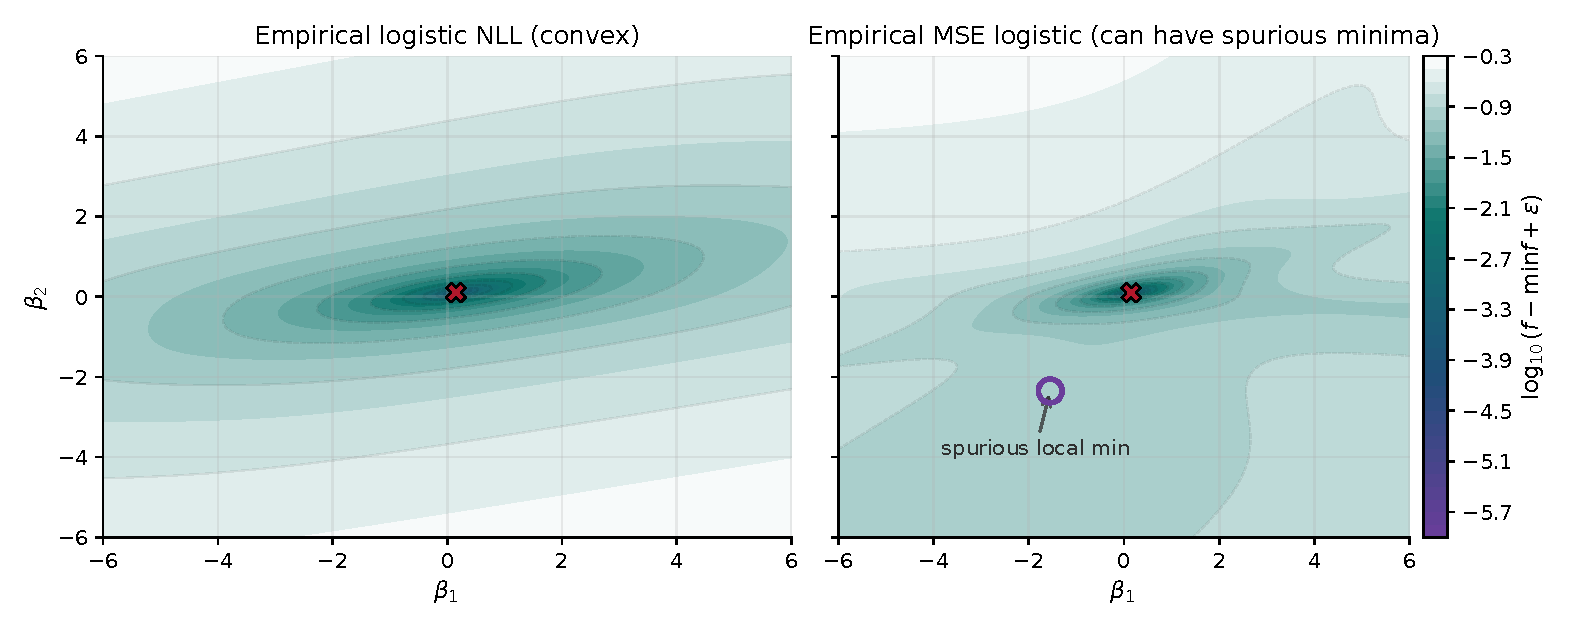
\includegraphics[width=\textwidth]{figures/handouts/convexity_optimization/fig_logistic_empirical_spurious}
  \caption{Empirical logistic landscapes on the dataset in \Cref{ex:logistic-empirical-spurious}.
  The plots show $\log_{10}(f-\min f+\varepsilon)$ for each objective.
  The red X marks the global minimizer in each panel.
  Left: the NLL is convex (one basin).
  Right: the squared-loss objective can have a spurious local minimum (circled), so a local method can get stuck.}
  \label{fig:logistic-empirical-spurious}
\end{figure}

\begin{figure}[t]
  \centering
  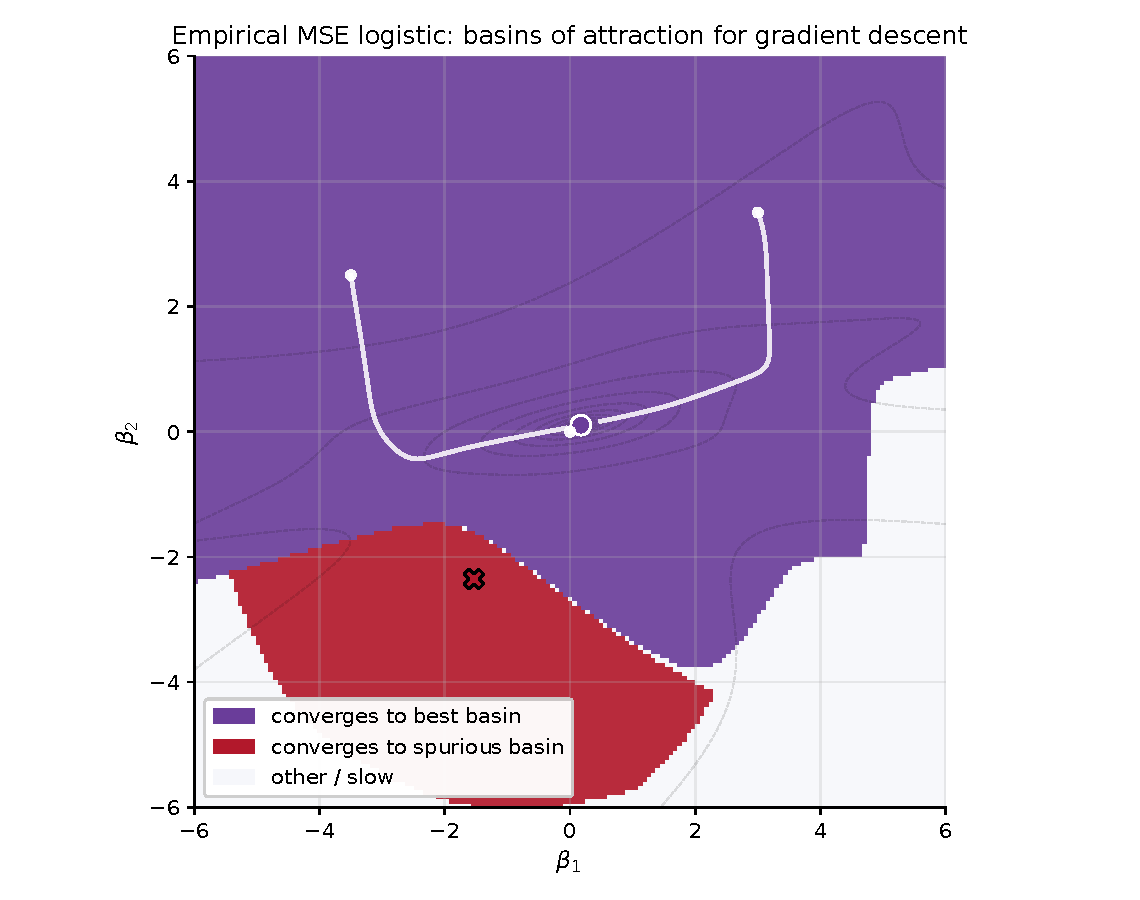
\includegraphics[width=0.92\textwidth]{figures/handouts/convexity_optimization/fig_logistic_empirical_basins}
  \caption{Basins of attraction for gradient descent on the empirical MSE-logistic objective in \Cref{ex:logistic-empirical-spurious}.
  The purple dot and red X mark the two local minimizers.
  Each initialization is colored by which local minimizer fixed-step GD (with $\eta=0.6$) converges to, and the overlaid paths show a few representative trajectories.}
  \label{fig:logistic-empirical-basins}
\end{figure}

Now assume a realizable population model:
\[
Y\mid X=x \sim \mathrm{Bernoulli}(p^\star(x)),
\qquad
p^\star(x) = \sigma(x^\top\beta^\star).
\]
Then the expected squared loss decomposes as
\[
\E\big[(Y-\sigma(X^\top\beta))^2\mid X\big]
= p^\star(X)(1-p^\star(X)) + \big(p^\star(X)-\sigma(X^\top\beta)\big)^2,
\]
so (up to an additive constant) the population objective becomes
\begin{equation}
R(\beta) = \E\big[(\sigma(X^\top\beta)-\sigma(X^\top\beta^\star))^2\big].
\label{eq:logistic-pop-risk}
\end{equation}

\begin{proposition}[One-point monotonicity in the realizable population squared-loss risk]
\label{prop:logistic-pop-one-point}
Assume $\E[\norm{X}_2]<\infty$, and let $R$ be as in \eqref{eq:logistic-pop-risk}. Then for all $\beta$,
\begin{equation}
\ip{\nabla R(\beta)}{\beta-\beta^\star} \ge 0.
\label{eq:one-point}
\end{equation}
In particular, along any ray $\beta(t)=\beta^\star+t(\beta-\beta^\star)$, the function $t\mapsto R(\beta(t))$ is nondecreasing for $t\ge 0$.
\end{proposition}

The next exercise isolates the population monotonicity calculation; structurally it plays the same role as the first-order convexity arguments in the Optimization unit.
\begin{exercise}[One-point monotonicity for realizable MSE-logistic]
\label{ex:logistic-one-point}
Prove \Cref{prop:logistic-pop-one-point}.
Let $\eta=X^\top\beta$ and $\eta^\star=X^\top\beta^\star$.
\begin{enumerate}[leftmargin=*]
  \item Differentiate under the expectation in \eqref{eq:logistic-pop-risk} to show that
  \[
  \nabla R(\beta)
  =2\,\E\Big[(\sigma(\eta)-\sigma(\eta^\star))\,\sigma'(\eta)\,X\Big].
  \]
  \item Show that
  \[
  \ip{\nabla R(\beta)}{\beta-\beta^\star}
  =2\,\E\Big[\sigma'(\eta)\,(\sigma(\eta)-\sigma(\eta^\star))(\eta-\eta^\star)\Big],
  \]
  and conclude it is nonnegative using only that $\sigma$ is increasing and $\sigma'\ge 0$.
  \item Deduce the ray-monotonicity statement by differentiating $g(t)=R(\beta^\star+t(\beta-\beta^\star))$.
\end{enumerate}
\end{exercise}

\SolutionBox[14]{%
\emph{Part (1).}
Differentiate \eqref{eq:logistic-pop-risk} under the expectation:
\[
R(\beta)=\E\big[(\sigma(X^\top\beta)-\sigma(X^\top\beta^\star))^2\big].
\]
Using the chain rule, $\nabla_\beta\sigma(X^\top\beta)=\sigma'(X^\top\beta)\,X$, hence
\[
\nabla R(\beta)
=2\,\E\Big[(\sigma(\eta)-\sigma(\eta^\star))\,\sigma'(\eta)\,X\Big],
\qquad
\eta=X^\top\beta,\ \eta^\star=X^\top\beta^\star.
\]

\emph{Part (2).}
Take the inner product with $(\beta-\beta^\star)$ and use $\ip{X}{\beta-\beta^\star}=\eta-\eta^\star$:
\[
\ip{\nabla R(\beta)}{\beta-\beta^\star}
=2\,\E\Big[\sigma'(\eta)\,(\sigma(\eta)-\sigma(\eta^\star))(\eta-\eta^\star)\Big].
\]
Since $\sigma'(\eta)\ge 0$ and $\sigma$ is increasing, we have
$(\sigma(\eta)-\sigma(\eta^\star))(\eta-\eta^\star)\ge 0$ pointwise.
Therefore the integrand is pointwise nonnegative, and the expectation is nonnegative as claimed.

\emph{Part (3) (ray monotonicity).}
For the ray $\beta(t)=\beta^\star+t(\beta-\beta^\star)$, define $g(t)=R(\beta(t))$.
By the chain rule,
\[
g'(t)=\ip{\nabla R(\beta(t))}{\beta-\beta^\star}\ge 0,
\]
so $t\mapsto R(\beta(t))$ is nondecreasing for $t\ge 0$.
(The argument uses only that the link is increasing with nonnegative derivative, so it holds for any such link function.)%
}

\begin{corollary}[Realizable population MSE-logistic has no spurious local minima]
\label{cor:logistic-pop-no-spurious}
Under the assumptions of \Cref{prop:logistic-pop-one-point}, every local minimizer of the realizable population risk $R$ in \eqref{eq:logistic-pop-risk} is global.
If in addition $\E[XX^\top]\succ 0$, then the unique global minimizer is $\beta^\star$.
\end{corollary}

\begin{exercise}[Stationarity + one-point monotonicity $\Rightarrow$ no spurious local minima]
\label{ex:logistic-one-point-no-spurious}
Prove \Cref{cor:logistic-pop-no-spurious} from \Cref{prop:logistic-pop-one-point}.
\begin{enumerate}[leftmargin=*]
  \item Let $\bar\beta$ be a local minimizer. Since $R$ is differentiable, $\nabla R(\bar\beta)=0$.
  Combine this with \Cref{eq:one-point} to show that
  \[
    0
    = \ip{\nabla R(\bar\beta)}{\bar\beta-\beta^\star}
    = 2\,\E\Big[\sigma'(\bar\eta)\,(\sigma(\bar\eta)-\sigma(\eta^\star))(\bar\eta-\eta^\star)\Big],
  \]
  where $\bar\eta=X^\top\bar\beta$ and $\eta^\star=X^\top\beta^\star$.
  Conclude that $\sigma(X^\top\bar\beta)=\sigma(X^\top\beta^\star)$ almost surely.
  \item Deduce that $R(\bar\beta)=0$, so $\bar\beta$ is a global minimizer.
  \item For uniqueness: show that if $R(\beta)=0$, then $X^\top(\beta-\beta^\star)=0$ almost surely, and deduce $\beta=\beta^\star$ under $\E[XX^\top]\succ 0$.
\end{enumerate}
\end{exercise}

\SolutionBox[14]{%
\emph{Part (1).}
Let $\bar\beta$ be a local minimizer of the differentiable function $R$.
Then $\nabla R(\bar\beta)=0$.
Applying \Cref{prop:logistic-pop-one-point} at $\beta=\bar\beta$ gives
\[
0
= \ip{\nabla R(\bar\beta)}{\bar\beta-\beta^\star}
= 2\,\E\Big[\sigma'(\bar\eta)\,(\sigma(\bar\eta)-\sigma(\eta^\star))(\bar\eta-\eta^\star)\Big],
\qquad \bar\eta=X^\top\bar\beta,\ \eta^\star=X^\top\beta^\star.
\]
The integrand is pointwise nonnegative because $\sigma'(\bar\eta)\ge 0$ and $\sigma$ is increasing, so the expectation can vanish only if the integrand is zero almost surely.
Since $\sigma'(z)>0$ for every finite $z$, this implies
\[
(\sigma(\bar\eta)-\sigma(\eta^\star))(\bar\eta-\eta^\star)=0
\qquad\text{almost surely.}
\]
Because $\sigma$ is strictly increasing, the product above is zero if and only if $\bar\eta=\eta^\star$, equivalently $\sigma(X^\top\bar\beta)=\sigma(X^\top\beta^\star)$ almost surely.

\emph{Part (2).}
If $\sigma(X^\top\bar\beta)=\sigma(X^\top\beta^\star)$ almost surely, then the integrand in \eqref{eq:logistic-pop-risk} vanishes almost surely, so
\[
R(\bar\beta)=\E\big[(\sigma(X^\top\bar\beta)-\sigma(X^\top\beta^\star))^2\big]=0.
\]
Since $R(\beta^\star)=0$ as well, $\bar\beta$ is a global minimizer.

\emph{Part (3) (uniqueness).}
If $R(\beta)=0$, then
\[
\E\big[(\sigma(X^\top\beta)-\sigma(X^\top\beta^\star))^2\big]=0,
\]
so $\sigma(X^\top\beta)=\sigma(X^\top\beta^\star)$ almost surely.
Since $\sigma$ is strictly increasing, this implies $X^\top(\beta-\beta^\star)=0$ almost surely.
Taking expectations yields
$(\beta-\beta^\star)^\top\E[XX^\top](\beta-\beta^\star)=0$.
If $\E[XX^\top]\succ 0$, then the quadratic form is strictly positive unless $\beta=\beta^\star$, so $\beta^\star$ is the unique global minimizer.%
}

The population MSE-logistic risk is nonconvex, but it still has the simple geometry that moving away from $\beta^\star$ does not help along any ray from $\beta^\star$.
This is qualitatively different from objectives like ecological logistic regression (\Cref{sec:ecological-logistic}), where aggregation introduces intrinsic nonconvexity and the landscape can have many distinct basins even under a clean population model.

Even with this benign global geometry, gradient descent can be slow because of saturation and flat plateaus.
The one-point monotonicity in \Cref{prop:logistic-pop-one-point} is a global geometry guarantee, but it is not a rate guarantee.
Far from $\beta^\star$, the squared-loss logistic objective can become very flat because the logistic link saturates:
$\sigma(z)\to 0$ or $1$ and $\sigma'(z)\to 0$ as $|z|\to\infty$.
The squared-loss gradient carries a factor of $\sigma'(X^\top\beta)$, so when the model is very confident (large $|X^\top\beta|$), the gradient can be tiny even if the objective value is not close to its minimum.
This mirrors the ``confidence weights'' story for convex NLL objectives:
in logistic NLL, curvature is largest near the decision boundary, while very confident points contribute little.
For squared loss, that same saturation suppresses the \emph{descent signal} itself, producing plateaus where $\norm{\nabla R(\beta)}_2$ is small even though $R(\beta)-R(\beta^\star)$ is not.

\begin{proposition}[Realizable squared-loss logistic: arbitrarily flat far from $\beta^\star$]
\label{prop:logistic-pop-flat}
Assume $\E[\norm{X}_2]<\infty$ and let $R$ be the realizable population risk \eqref{eq:logistic-pop-risk}.
Define $g(t)=R(t\beta^\star)$ for $t\ge 1$.
Then:
\begin{enumerate}[leftmargin=*]
  \item $g$ is nondecreasing on $[1,\infty)$ and converges to a finite limit $g(\infty)$.
  \item $\lim_{t\to\infty} g'(t)=0$ and $\lim_{t\to\infty}\norm{\nabla R(t\beta^\star)}_2=0$.
  \item If $\Pr(X^\top\beta^\star\neq 0)>0$, then $g(\infty)>0$.
\end{enumerate}
In particular, there are directions along which the landscape becomes arbitrarily flat even though the excess risk stays bounded away from $0$.
\end{proposition}

\emph{Proof idea.} See Exercise~\ref{ex:logistic-plateau}.

\begin{exercise}[Prove the plateau]
\label{ex:logistic-plateau}
In the realizable population model, let $g(t)=R(t\beta^\star)$ for $t\ge 1$.
\begin{enumerate}[leftmargin=*]
  \item Show that
  \[
    g'(t)=2\,\E\big[(\sigma(t\eta^\star)-\sigma(\eta^\star))\,\sigma'(t\eta^\star)\,\eta^\star\big],
    \qquad \eta^\star=X^\top\beta^\star,
  \]
  and conclude that $g$ is nondecreasing (hence $g(t)\to g(\infty)$ since $0\le g(t)\le 1$).
  \item Show that $g'(t)\to 0$ and $\nabla R(t\beta^\star)\to 0$ as $t\to\infty$.
  Interpret this as: \emph{without} a PL/strong-convexity-type condition, small gradient does not imply near-optimality.
  \item Assume $\Pr(\eta^\star\neq 0)>0$.
  Show that $g(\infty)>0$.
\end{enumerate}
\end{exercise}

\SolutionBox[12]{%
Write $\eta^\star=X^\top\beta^\star$ so that $g(t)=\E[(\sigma(t\eta^\star)-\sigma(\eta^\star))^2]$.

\emph{Part (1).}
Differentiate under the expectation:
by the chain rule,
\[
\frac{d}{dt}\sigma(t\eta^\star)=\sigma'(t\eta^\star)\,\eta^\star,
\]
so
\[
g'(t)
=\E\Big[2(\sigma(t\eta^\star)-\sigma(\eta^\star))\cdot \sigma'(t\eta^\star)\,\eta^\star\Big]
=2\,\E\big[(\sigma(t\eta^\star)-\sigma(\eta^\star))\,\sigma'(t\eta^\star)\,\eta^\star\big].
\]
For $t\ge 1$, $\sigma(t\eta^\star)-\sigma(\eta^\star)$ has the same sign as $(t-1)\eta^\star$ since $\sigma$ is increasing.
Because $\sigma'\ge 0$, the integrand is pointwise nonnegative, hence $g'(t)\ge 0$ and $g$ is nondecreasing.
Since $g(t)\in[0,1]$, it follows that $g(t)\to g(\infty)$ for some finite limit $g(\infty)$.

\emph{Part (2).}
For each fixed $\eta^\star\neq 0$, we have $t\eta^\star\to \pm\infty$ and therefore $\sigma'(t\eta^\star)\to 0$ as $t\to\infty$.
Also,
\[
\big|(\sigma(t\eta^\star)-\sigma(\eta^\star))\,\sigma'(t\eta^\star)\,\eta^\star\big|
\le \sigma'(0)\,|\eta^\star|
\le \sigma'(0)\,\norm{\beta^\star}_2\,\norm{X}_2,
\]
which is integrable since $\E[\norm{X}_2]<\infty$.
We will use the following standard fact: if random variables $Z_t$ satisfy $|Z_t|\le W$ with $\E[W]<\infty$ and $Z_t\to 0$ almost surely, then $\E[Z_t]\to 0$.
Applying this fact here gives $g'(t)\to 0$ as $t\to\infty$.

\smallskip
Similarly, differentiating \eqref{eq:logistic-pop-risk} gives
\[
\nabla R(t\beta^\star)
=2\,\E\big[(\sigma(t\eta^\star)-\sigma(\eta^\star))\,\sigma'(t\eta^\star)\,X\big].
\]
The integrand norm is bounded by $2\sigma'(0)\norm{X}_2$, and for each fixed $X$ the factor $\sigma'(t\eta^\star)$ tends to $0$ (or the bracketed term vanishes when $\eta^\star=0$), so the same reasoning lets us pass the limit through the expectation and conclude $\nabla R(t\beta^\star)\to 0$.

\emph{Part (3).}
As $t\to\infty$ we have $\sigma(t\eta^\star)\to 1$ when $\eta^\star>0$, $\sigma(t\eta^\star)\to 0$ when $\eta^\star<0$, and $\sigma(t\eta^\star)=\sigma(\eta^\star)=1/2$ when $\eta^\star=0$.
Since $0\le (\sigma(t\eta^\star)-\sigma(\eta^\star))^2\le 1$, we can apply the same fact (with $W=1$) to pass the limit through the expectation and obtain
\[
g(\infty)=\E\Big[(1-\sigma(\eta^\star))^2\mathbf{1}\{\eta^\star>0\} + \sigma(\eta^\star)^2\mathbf{1}\{\eta^\star<0\}\Big].
\]
If $\Pr(\eta^\star\neq 0)>0$, then the integrand is strictly positive on $\{\eta^\star\neq 0\}$, so $g(\infty)>0$.

Along this ray, the risk can remain bounded away from $0$ while the gradient (and directional derivative) goes to $0$.
Without a condition like PL/strong convexity, a small gradient does not by itself certify near-optimality.
}

Conditions like strong convexity or the PL inequality (\Cref{def:pl-inequality}) prevent this phenomenon: they rule out large flat regions away from the optimum by relating gradient size to suboptimality.
\Cref{prop:logistic-pop-flat} shows the realizable squared-loss logistic risk does not have such a global guarantee in general.

In the realizable population model, the one-point monotonicity in \Cref{prop:logistic-pop-one-point} is a \emph{global} geometric statement.
To get an actual rate for gradient descent, we also need a \emph{local curvature} condition near $\beta^\star$.
One simple sufficient condition is bounded features, which implies local strong convexity (hence a linear rate) around the optimum.

\begin{proposition}[Local linear convergence of gradient descent near $\beta^\star$]
\label{prop:logistic-pop-local-rate}
Assume $\E[XX^\top]\succeq \lambda I_d$ and $\norm{X}_2\le R$ almost surely for some $\lambda,R>0$.
Then at $\beta^\star$,
\[
\Hess R(\beta^\star)\succeq m_0 I_d,
\qquad
m_0 = 2\,\sigma'(R\norm{\beta^\star}_2)^2\,\lambda,
\]
and there exist $r>0$ and constants $0<m\le L<\infty$ such that the population risk $R$ in \eqref{eq:logistic-pop-risk} is $m$-strongly convex and $L$-smooth on the ball $\{\beta:\ \norm{\beta-\beta^\star}_2\le r\}$.
Consequently, gradient descent with step size $1/L$ initialized in this ball satisfies
\[
R(\beta^{(k)})-R(\beta^\star)
\le \left(1-\frac{m}{L}\right)^k\bigl(R(\beta^{(0)})-R(\beta^\star)\bigr)
\qquad\text{(see \citealp[\S9.3]{boyd_vandenberghe_2004_convex}).}
\]
\end{proposition}

\begin{proof}
Differentiate \eqref{eq:logistic-pop-risk} twice.
At $\beta=\beta^\star$, the cross term vanishes and the Hessian simplifies to
\[
\Hess R(\beta^\star)=2\,\E\big[\sigma'(X^\top\beta^\star)^2\,XX^\top\big].
\]
Since $\norm{X^\top\beta^\star}\le \norm{X}_2\norm{\beta^\star}_2\le R\norm{\beta^\star}_2$ almost surely, we have
$\sigma'(X^\top\beta^\star)\ge \sigma'(R\norm{\beta^\star}_2)>0$ almost surely (since $\sigma'$ is even and decreases with $|z|$), hence
\[
\Hess R(\beta^\star)\succeq 2\,\sigma'(R\norm{\beta^\star}_2)^2\,\E[XX^\top]\succeq 2\,\sigma'(R\norm{\beta^\star}_2)^2\,\lambda I_d.
\]
This is the claimed bound with $m_0=2\,\sigma'(R\norm{\beta^\star}_2)^2\,\lambda$.
Because $R$ is twice continuously differentiable and $\norm{X}_2\le R$ almost surely, $\Hess R(\beta)$ varies continuously in $\beta$ and is bounded on compact sets.
Therefore, on a sufficiently small ball around $\beta^\star$, the Hessian is bounded below by (say) $\tfrac12 m_0 I_d$ and above by $L I_d$ for some finite $L$, which gives local strong convexity and smoothness.
The linear convergence rate for gradient descent on an $m$-strongly convex and $L$-smooth function is standard (cited above).
\end{proof}

Under misspecification, hard multimodality can return.
If $p^\star(x)$ is not representable as $\sigma(x^\top\beta)$ (e.g.\ marginalizing over latent classes can yield mixtures of logits), then \eqref{eq:one-point} need not hold, and the population squared-loss risk can become bimodal with spurious local minima.
Benign global geometry often hinges on model and data assumptions.
This is one reason MLE (convex NLL) is often more stable than squared-loss fitting in logistic-type binary regression models.

\begin{example}[Misspecification can create a spurious local minimum for squared-loss logistic regression]
\label{ex:logistic-misspecified-spurious}
Consider a 1D feature $X$ that takes values $\{-2,-1,1,2\}$ with equal probability, and parameterize $\beta=(\beta_0,\beta_1)$ so that $q_\beta(x)=\sigma(\beta_0+\beta_1 x)$.
Let the true conditional probabilities be
\[
p^\star(-2)=0.49,\quad p^\star(-1)=0.87,\quad p^\star(1)=0.92,\quad p^\star(2)=0.36.
\]
This $p^\star$ is not representable as $q_\beta$, since it is not monotone in $x$.

For the population squared-loss risk $R_{\mathrm{MSE}}(\beta)=\E[(q_\beta(X)-p^\star(X))^2]$, a direct evaluation shows two distinct basins:
numerically, evaluating $R_{\mathrm{MSE}}$ on a grid reveals a global minimizer and a spurious local minimizer.
See \Cref{fig:logistic-landscape-2d}.
\end{example}

\begin{figure}[t]
  \centering
  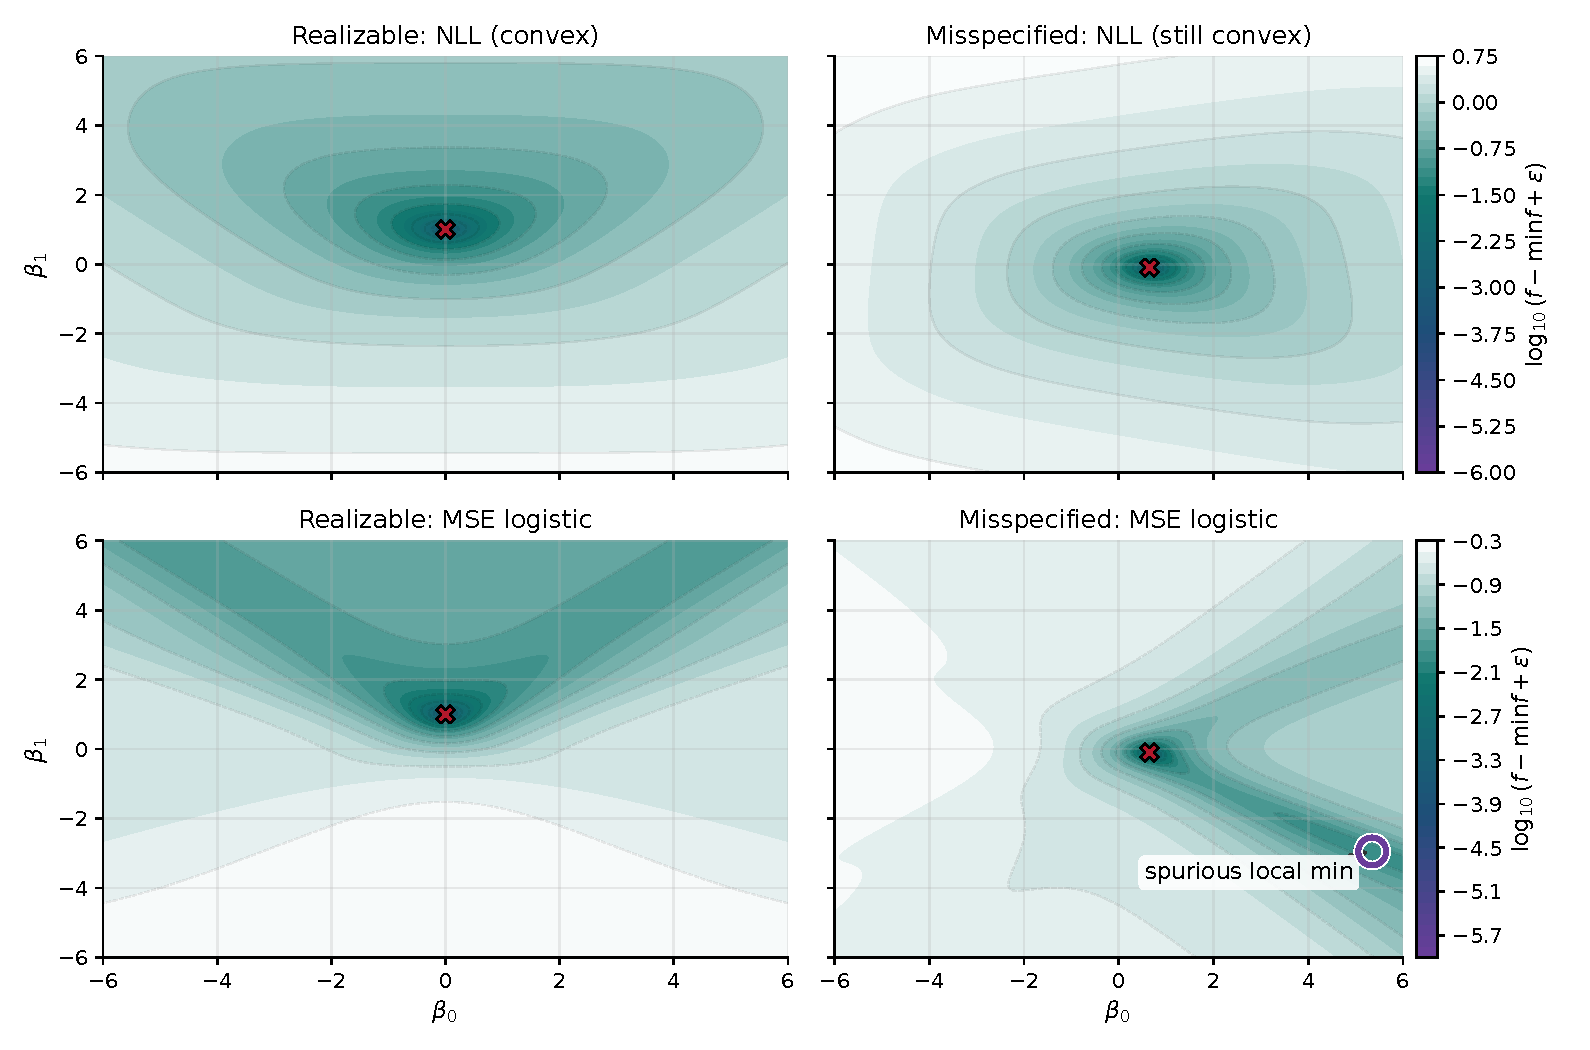
\includegraphics[width=\textwidth]{figures/handouts/convexity_optimization/fig_logistic_landscape_2d}
  \caption{A consistent contourf view of logistic landscapes in a 2D parameterization $\beta=(\beta_0,\beta_1)$.
  The plots show $\log_{10}(f-\min f+\varepsilon)$ for each objective, which makes basins comparable across panels.
  The red X marker indicates the global minimizer in each panel; in the bottom-right plot, the circled point is a spurious local minimum.
  In this example, the NLL landscape is unimodal in both realizable and misspecified settings, while the squared-loss landscape can develop extra basins under misspecification.}
  \label{fig:logistic-landscape-2d}
\end{figure}

% ------------------------------------------------------------
Example~I separates three distinct regimes.
Empirical MSE-logistic can create spurious basins; the realizable population risk has no spurious local minima but can still be slow because of broad plateaus; and misspecification can bring back genuinely wrong stable basins.
The response depends on the regime: use a stable objective when possible, use damping or line search when curvature is unreliable, and use restarts or stronger initializations when multiple basins are present.

% ------------------------------------------------------------
\section[Example II (phase retrieval)]{Example II: multimodality from symmetry, but only global optima in phase retrieval}
\label{sec:phase-retrieval}

In coherent diffraction imaging, optics, and astronomy, sensors measure intensities and lose phase.
A canonical real model is \emph{phase retrieval}:
\[
y_i = (a_i^\top x^\star)^2,\qquad i=1,\dots,m,
\]
where $x^\star\in\R^d$ is the unknown signal and $a_i$ are known sensing vectors.
A standard nonconvex least-squares objective is
\begin{equation}
F(x)=\frac{1}{4m}\sum_{i=1}^m\big((a_i^\top x)^2 - y_i\big)^2.
\label{eq:phase-empirical}
\end{equation}
This objective is nonconvex for structural reasons (it involves squares of linear forms),
and it is \emph{inherently} multimodal because $x^\star$ and $-x^\star$ generate the same data.

Like squared-loss logistic regression, phase retrieval is a smooth, nonconvex least-squares objective.
But here the nonconvexity is driven primarily by a \emph{symmetry}: $x^\star$ and $-x^\star$ generate the same data.
In population (for Gaussian designs), this symmetry produces multiple global optima but \emph{no} suboptimal local minima; the remaining stationary points are saddles.
This is ``benign'' nonconvexity (a strict-saddle picture), and it contrasts with ecological logistic regression (\Cref{sec:ecological-logistic}), where aggregation creates intrinsic nonconvexity and can lead to many distinct basins.
This ``benign geometry'' picture (multiple equivalent global minimizers; strict saddles elsewhere) appears broadly in modern tractable nonconvex problems; see \citet[\S2]{sun_qu_wright_2015_nonconvex_not_scary} and \citet[\S1]{zhang_qu_wright_2020_symmetry_geometry}.

\begin{figure}[t]
  \centering
  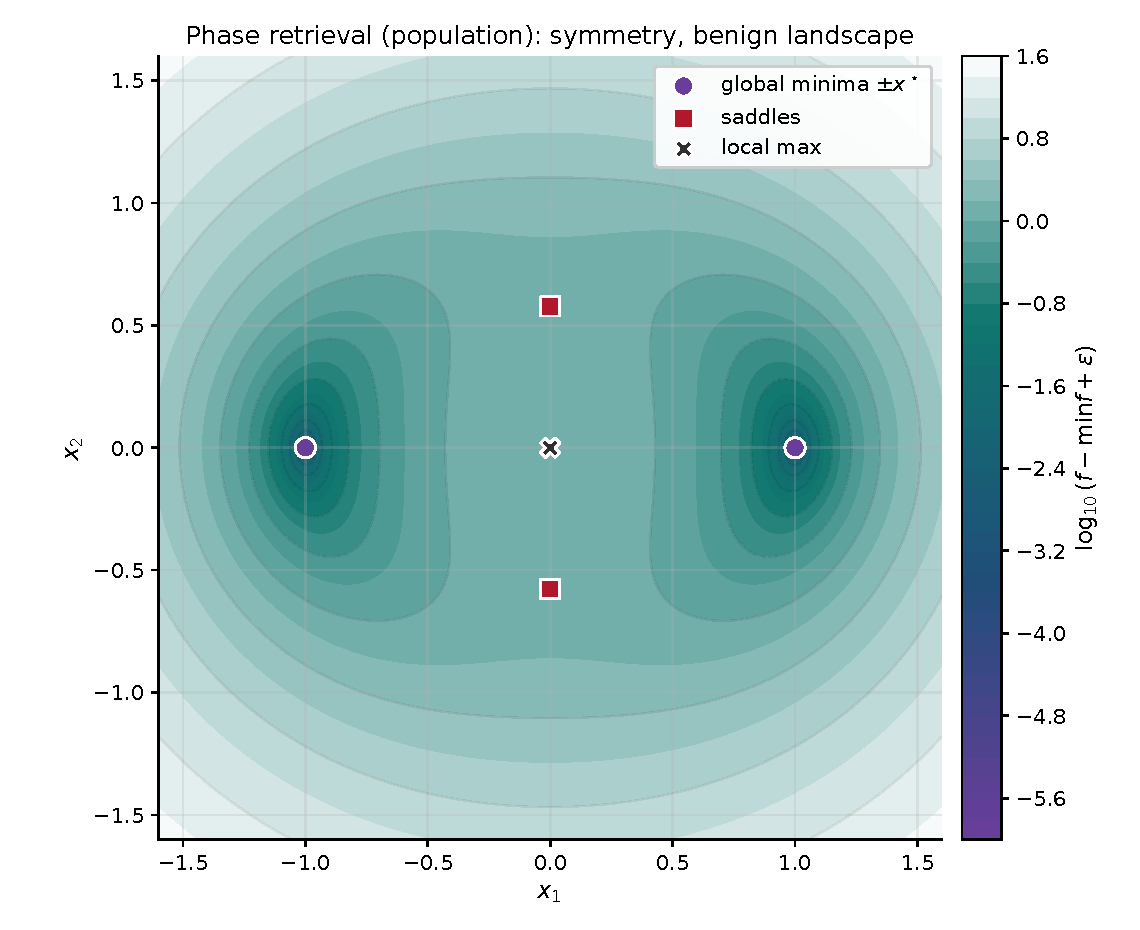
\includegraphics[width=0.86\textwidth]{figures/handouts/convexity_optimization/fig_phase_retrieval_landscape}
  \caption{Population phase retrieval in $d=2$: the landscape is nonconvex and symmetric ($x\sim -x$), but the only local minima are the two global minima $\pm x^\star$; other critical points are saddles or a local maximum at the origin.}
  \label{fig:phase-retrieval-landscape}
\end{figure}

For a clean population model, assume $a\sim N(0,I_d)$ and consider the \emph{population} objective
\begin{equation}
  f(x)=\frac12\,\E\Big[\big((a^\top x)^2 - (a^\top x^\star)^2\big)^2\Big].
  \label{eq:phase-pop}
\end{equation}

\begin{proposition}[Population phase retrieval: nonconvex but no spurious local minima]
\label{prop:phase-retrieval-benign}
For $f$ in \eqref{eq:phase-pop},
\begin{equation}
  f(x)
  =\frac{3}{2}\norm{x}^4 - \norm{x}^2\norm{x^\star}^2 - 2\ip{x}{x^\star}^2 + \frac{3}{2}\norm{x^\star}^4,
  \label{eq:phase-pop-closed-form}
\end{equation}
and the stationary points are:
\begin{enumerate}[leftmargin=*]
  \item global minima $x=\pm x^\star$ (value $0$),
  \item a local maximum at $x=0$,
  \item a saddle set $\{x:\ x\perp x^\star,\ \norm{x}=\norm{x^\star}/\sqrt{3}\}$.
\end{enumerate}
In particular, every local minimum is global.
\end{proposition}

\begin{exercise}[Phase retrieval: derive and classify the population stationary points]
\label{ex:phase-pop-derivation}
Prove \Cref{prop:phase-retrieval-benign}.
\begin{enumerate}[leftmargin=*]
  \item Expand \eqref{eq:phase-pop} and use the Gaussian fourth-moment identities
  \[
  \E[(a^\top u)^4]=3\norm{u}^4,
  \qquad
  \E[(a^\top u)^2(a^\top v)^2]=\norm{u}^2\norm{v}^2 + 2\ip{u}{v}^2,
  \]
  to obtain \eqref{eq:phase-pop-closed-form}.
  \item Differentiate \eqref{eq:phase-pop-closed-form} to get an explicit formula for $\nabla f(x)$.
  \item Solve $\nabla f(x)=0$ by decomposing $x=\alpha x^\star + u$ with $u\perp x^\star$.
  \item Classify the stationary points as global minima, a local maximum, and a saddle set.
\end{enumerate}
\end{exercise}

\SolutionBox[22]{%
\emph{Part (1) (closed form).}
Expanding the square in \eqref{eq:phase-pop} gives
\[
f(x)
=\frac12\,\E\big[(a^\top x)^4\big]
\;-\;\E\big[(a^\top x)^2(a^\top x^\star)^2\big]
\;+\;\frac12\,\E\big[(a^\top x^\star)^4\big].
\]
Apply the stated Gaussian fourth-moment identities with $u=x$ and $v=x^\star$ to get
\[
\E[(a^\top x)^4]=3\norm{x}^4,\qquad
\E[(a^\top x^\star)^4]=3\norm{x^\star}^4,
\]
and
\[
\E[(a^\top x)^2(a^\top x^\star)^2]=\norm{x}^2\norm{x^\star}^2 + 2\ip{x}{x^\star}^2.
\]
Substituting yields \eqref{eq:phase-pop-closed-form}.

\emph{Part (2) (gradient).}
Differentiate \eqref{eq:phase-pop-closed-form}:
\[
\nabla f(x)
= 6\norm{x}^2 x - 2\norm{x^\star}^2 x - 4\ip{x}{x^\star}x^\star
= (6\norm{x}^2-2\norm{x^\star}^2)x - 4\ip{x}{x^\star}x^\star.
\]

\emph{Part (3) (stationary points).}
Let $r=\norm{x^\star}_2$ and decompose $x=\alpha x^\star + u$ with $u\perp x^\star$.
Then $\ip{x}{x^\star}=\alpha r^2$ and $\norm{x}^2=\alpha^2r^2+\norm{u}^2$.
Setting $\nabla f(x)=0$ and matching the $u$ and $x^\star$ components gives
\[
(6\norm{x}^2-2r^2)\,u=0,
\qquad
\alpha\,(6\norm{x}^2-6r^2)=0.
\]
If $u=0$, then either $\alpha=0$ (so $x=0$) or $\norm{x}^2=r^2$ (so $\alpha=\pm 1$ and $x=\pm x^\star$).
If $u\neq 0$, then the first equation forces $\norm{x}^2=r^2/3$, and the second forces $\alpha=0$, hence
$x\perp x^\star$ and $\norm{x}=r/\sqrt{3}$.
This gives exactly the stationary-point list in \Cref{prop:phase-retrieval-benign}.

\emph{Part (4) (classification).}
Since $f$ in \eqref{eq:phase-pop} is an expectation of a square, $f(x)\ge 0$ for all $x$.
Also $f(\pm x^\star)=0$, so $\pm x^\star$ are global minima.

For $x=0$, the expansion \eqref{eq:phase-pop-closed-form} shows
\[
f(0)-f(x)= r^2\norm{x}^2 + 2\ip{x}{x^\star}^2 - \frac{3}{2}\norm{x}^4,
\]
which is strictly positive for all sufficiently small $x\neq 0$ (the quadratic term dominates), so $x=0$ is a local maximum.

Finally, if $x\perp x^\star$ and $\norm{x}=r/\sqrt{3}$, then the univariate restriction $t\mapsto f(x+t x^\star)$ has negative second derivative at $t=0$, so there is a direction of negative curvature.
Hence these points are saddles, and every local minimum is global.%
}

This is symmetry-driven nonconvexity with a strict-saddle geometry:
every non-optimal stationary point has a direction of negative curvature.

Phase retrieval is typically approached via the two-stage template in \Cref{alg:two-stage-template}:
use a cheap global initializer, then run a local method.
In the Gaussian model, there is a clean way to build a provably good direction estimate from a simple moment identity.
Assume the noiseless Gaussian design model $a_i \stackrel{\mathrm{iid}}{\sim} N(0,I_d)$ with measurements $y_i=(a_i^\top x^\star)^2$.
Define the \emph{spectral matrix}
\[
  Y = \frac{1}{m}\sum_{i=1}^m y_i a_i a_i^\top.
\]
Also define the radius estimate
\[
  \hat r^2 = \frac{1}{m}\sum_{i=1}^m y_i,
\]
which satisfies $\E[\hat r^2]=\norm{x^\star}_2^2$.
If $\hat u$ is a unit-norm top eigenvector of $Y$, then the standard spectral initializer is $x^{(0)}=\hat r\,\hat u$.

The next proposition explains why this initialization is reasonable.
It shows that (i) the population matrix $\E[Y]$ has a unique leading eigenvector in the $x^\star$ direction, and (ii) if the empirical $Y$ is close to $\E[Y]$ in operator norm then its leading eigenvector must be close to $\pm x^\star/\norm{x^\star}_2$.
(Here $\norm{M}_{\mathrm{op}}$ denotes the operator norm, i.e.\ the largest absolute eigenvalue for a symmetric matrix $M$.)

\begin{proposition}[Gaussian phase retrieval: why the spectral initializer points at $x^\star$]
\label{prop:phase-spectral-init}
Assume $x^\star\neq 0$, let $a\sim N(0,I_d)$, and set $y=(a^\top x^\star)^2$.
Write $r=\norm{x^\star}_2$ and $u^\star=x^\star/r$.
Define the population matrix
\[
  Y_{\mathrm{pop}} = \E\big[y\,a a^\top\big]
  = \E\big[(a^\top x^\star)^2 a a^\top\big].
\]
Then
\[
  Y_{\mathrm{pop}}=r^2 I_d + 2x^\star(x^\star)^\top,
\]
so the unique leading eigenvector of $Y_{\mathrm{pop}}$ is $u^\star$.
Moreover, if $Y$ is any symmetric matrix satisfying
\[
\norm{Y-Y_{\mathrm{pop}}}_{\mathrm{op}} \le \varepsilon\, r^2
\qquad\text{for some }\varepsilon\in(0,1),
\]
then for every unit-norm leading eigenvector $\hat u$ of $Y$ there exists a sign $s\in\{\pm 1\}$ such that
$\norm{\hat u-su^\star}_2\le \sqrt{2\varepsilon}$.
\end{proposition}

\begin{exercise}[Phase retrieval: why spectral initialization points at $x^\star$]
\label{ex:phase-spectral-spike}
Prove \Cref{prop:phase-spectral-init}.
Conclude that if the empirical matrix $Y$ is close to $Y_{\mathrm{pop}}$ in operator norm, then its top eigenvector is close to $\pm u^\star$ and the spectral initializer $x^{(0)}=\hat r\,\hat u$ is close to $\pm x^\star$.
\emph{Hint:} to compute $Y_{\mathrm{pop}}$, you can either compute entries using the Gaussian fourth-moment identity
$\E[a_i a_j a_k a_\ell]=\delta_{ij}\delta_{k\ell}+\delta_{ik}\delta_{j\ell}+\delta_{i\ell}\delta_{jk}$,
or compute the entries directly by expanding.
For the perturbation bound, compare quadratic forms $v^\top Y v$ and use $|v^\top (Y-Y_{\mathrm{pop}}) v|\le \norm{Y-Y_{\mathrm{pop}}}_{\mathrm{op}}$ for unit $v$.
Finally, explain in a sentence why one expects $\norm{Y-Y_{\mathrm{pop}}}_{\mathrm{op}}$ to be small when $m$ is large in the Gaussian model.
\end{exercise}

\SolutionBox[20]{%
Write $u=x^\star$ and expand $y=(a^\top u)^2=\sum_{k,\ell} u_k u_\ell a_k a_\ell$.
For each entry $(i,j)$,
\[
\E\!\big[y\,a_i a_j\big]
=\sum_{k,\ell} u_k u_\ell\,\E[a_i a_j a_k a_\ell]
=\sum_{k,\ell} u_k u_\ell\bigl(\delta_{ij}\delta_{k\ell}+\delta_{ik}\delta_{j\ell}+\delta_{i\ell}\delta_{jk}\bigr).
\]
The first term gives $\delta_{ij}\sum_k u_k^2=\delta_{ij}\norm{u}_2^2$.
The second and third terms each give $u_i u_j$.
Thus $\E[y\,a_i a_j]=\norm{u}_2^2\,\delta_{ij}+2u_i u_j$, i.e.
$Y_{\mathrm{pop}}=\norm{u}_2^2 I_d + 2uu^\top$.

For eigenvalues, note that $Y_{\mathrm{pop}}u=(\norm{u}_2^2+2\norm{u}_2^2)u=3\norm{u}_2^2 u$.
If $w\perp u$, then $uu^\top w=0$ so $Y_{\mathrm{pop}}w=\norm{u}_2^2 w$.
Hence the unique top eigenspace is $\mathrm{span}\{u\}$.

Let $r=\norm{u}_2$ and $u^\star=u/r$.
Let $\hat u$ be a unit top eigenvector of $Y$.
Write $E=Y-Y_{\mathrm{pop}}$ and assume $\norm{E}_{\mathrm{op}}\le \varepsilon r^2$.
Then
\[
\hat u^\top Y_{\mathrm{pop}} \hat u
= \hat u^\top Y \hat u - \hat u^\top E \hat u
\ge \lambda_{\max}(Y) - \norm{E}_{\mathrm{op}}
\ge (u^\star)^\top Y u^\star - \norm{E}_{\mathrm{op}}
\ge 3r^2 - 2\varepsilon r^2.
\]
On the other hand,
$
\hat u^\top Y_{\mathrm{pop}} \hat u
= r^2 + 2r^2\,|\ip{\hat u}{u^\star}|^2.
$
Combining gives $|\ip{\hat u}{u^\star}|^2\ge 1-\varepsilon$.
Choosing the sign that maximizes the inner product,
\[
\min\{\norm{\hat u-u^\star}_2,\norm{\hat u+u^\star}_2\}^2
=2\bigl(1-|\ip{\hat u}{u^\star}|\bigr)
\le 2\bigl(1-|\ip{\hat u}{u^\star}|^2\bigr)
\le 2\varepsilon.
\]

The matrix $Y$ is an empirical average of i.i.d.\ symmetric matrices with mean $Y_{\mathrm{pop}}$.
To make this quantitative in high dimensions, one uses concentration inequalities for random matrices to bound $\norm{Y-Y_{\mathrm{pop}}}_{\mathrm{op}}$ with high probability; see \citet[\S2.2]{zhang_qu_wright_2020_symmetry_geometry} for discussion and references.
These probability tools are largely orthogonal to our focus here.%
}

Once you have an initialization that is close to $\pm x^\star$, the local stage behaves like the convex story again.
In the Gaussian population objective, $\pm x^\star$ are not only global minima: they are \emph{locally strongly convex} minima, so the standard local strong-convexity analysis from the Optimization unit gives a linear rate while the iterates remain in that neighborhood.

\begin{exercise}[Phase retrieval: local convexity near $\pm x^\star$ in the population objective]
\label{ex:phase-pop-local-strong-convex}
For the population objective $f$ in \eqref{eq:phase-pop-closed-form}, compute the Hessian $\Hess f(x)$ and show that
\[
\Hess f(x^\star)=4\norm{x^\star}_2^2 I_d + 8x^\star(x^\star)^\top.
\]
Deduce the eigenvalues of $\Hess f(x^\star)$ and interpret this as a local condition-number statement near $x^\star$.
\end{exercise}

\SolutionBox[12]{%
Differentiate the gradient formula in the solution to \Cref{ex:phase-pop-derivation}:
for $x\in\R^d$,
\[
\Hess f(x)=12xx^\top + (6\norm{x}_2^2-2\norm{x^\star}_2^2)I_d - 4x^\star(x^\star)^\top.
\]
At $x=x^\star$ this becomes
\[
\Hess f(x^\star)=(12-4)x^\star(x^\star)^\top + 4\norm{x^\star}_2^2 I_d
=8x^\star(x^\star)^\top + 4\norm{x^\star}_2^2 I_d.
\]
Along $u^\star=x^\star/\norm{x^\star}_2$ the eigenvalue is $12\norm{x^\star}_2^2$, and along any direction orthogonal to $x^\star$ the eigenvalue is $4\norm{x^\star}_2^2$.
So near $x^\star$ the population objective is well conditioned (local condition number $3$), which is exactly the regime where local methods behave like in the convex case.%
}

These pieces give the standard Gaussian-model story:
spectral initialization supplies a direction close to $\pm x^\star$, and the local geometry near $\pm x^\star$ is strongly convex, so local methods converge quickly once initialized there.
Rigorous finite-sample analyses follow this template; see \citet[\S2.2]{zhang_qu_wright_2020_symmetry_geometry} and references therein.

Phase retrieval shows a different kind of nonconvexity.
The sign symmetry creates multiple optima, but they are equivalent, and the remaining stationary points are saddles rather than bad local minima.
The right response is therefore not exhaustive global search; it is a coarse initializer, such as a spectral method, followed by local refinement inside the basin of $\pm x^\star$.



% ------------------------------------------------------------
\section[Example III (ecological logistic)]{Example III: hard nonconvexity from aggregation in ecological logistic regression}
\label{sec:ecological-logistic}

In some applications we observe covariates at the unit level but only aggregated outcomes.
For example, we might see covariates $x_{g,1},\dots,x_{g,n_g}$ for individuals in a group (a precinct, a cohort, a batch),
but instead of observing the binary outcomes $Y_{g,i}\in\{0,1\}$ we only observe the group total
\[
Z_g = \sum_{i=1}^{n_g} Y_{g,i}.
\]
Many different binary vectors $(Y_{g,1},\dots,Y_{g,n_g})$ can produce the same total $Z_g$, so the likelihood for $\beta$ must marginalize over a large discrete set of latent ``assignments.''

Assume a logistic model at the unit level:
\[
\Pr(Y_{g,i}=1\mid x_{g,i},\beta)=\sigma(x_{g,i}^\top\beta),
\qquad i=1,\dots,n_g,
\]
with conditional independence across $i$ given the covariates.
Write $p_{g,i}(\beta)=\sigma(x_{g,i}^\top\beta)$.
Then $Z_g$ is a sum of independent but non-identically distributed Bernoulli random variables (a Poisson--binomial model), and the marginal likelihood contains $\binom{n_g}{z_g}$ terms.
The resulting negative log-likelihood is typically nonconvex in $\beta$.
This combinatorial marginalization also creates a separate difficulty that is easy to miss if we focus only on the geometry:
when $n_g$ is large, the likelihood term $\Pr(Z_g=z_g\mid x_{g,1},\dots,x_{g,n_g},\beta)$ can be expensive to evaluate repeatedly inside an optimizer.
The naive computation is literally a sum over $\binom{n_g}{z_g}$ assignments (as in \Cref{ex:eco-logistic-nonconvex}), which is intractable for large groups.
This ``optimization + marginalization'' pattern is common in latent-variable models: hard landscapes and expensive objective evaluations can come together.

An empirical negative log-likelihood objective for $G$ independent groups is
\begin{equation}
  f(\beta)
  =
  -\frac{1}{G}\sum_{g=1}^G \log \Pr(Z_g=z_g \mid x_{g,1},\dots,x_{g,n_g},\beta).
  \label{eq:eco-logistic-obj}
\end{equation}
Two edge cases are instructive.
In the special case where the covariates are constant within each group ($x_{g,i}\equiv x_g$), we have
$Z_g\sim \mathrm{Binomial}(n_g,\sigma(x_g^\top\beta))$, and \eqref{eq:eco-logistic-obj} reduces to the usual convex binomial logistic-regression objective from the Optimization unit.
At the other extreme, if $d=1$ with $\beta=(\beta_0,\beta_1)$ and each group contains covariates in $\pm$ pairs (for every $x$ the value $-x$ appears with the same multiplicity), then the marginal likelihood is symmetric in the slope: it is unchanged under $\beta_1\mapsto -\beta_1$.
This kind of symmetry reflects a genuine non-identifiability from totals alone.

\begin{exercise}[Ecological logistic regression: two easy special cases]
\label{ex:eco-logistic-edge-cases}
\begin{enumerate}[leftmargin=*]
  \item Suppose $x_{g,i}\equiv x_g$ within each group.
  Show that $Z_g\sim \mathrm{Binomial}(n_g,\sigma(x_g^\top\beta))$ and conclude that the corresponding negative log-likelihood is convex in $\beta$.
  \item Assume $d=1$ with $\beta=(\beta_0,\beta_1)$ and suppose the multiset $\{x_1,\dots,x_n\}$ is symmetric: for every $x$ it contains $-x$ with the same multiplicity.
  Show that, for every $z$,
  \[
    \Pr(Z=z\mid x_1,\dots,x_n,(\beta_0,\beta_1))
    =
    \Pr(Z=z\mid x_1,\dots,x_n,(\beta_0,-\beta_1)).
  \]
  Conclude that the likelihood for $\beta_1$ is an even function, so the sign of the slope is not identifiable from $Z$ alone in such a balanced design.
\end{enumerate}
\end{exercise}

\SolutionBox[14]{%
\emph{Part (1).}
If $x_{g,i}\equiv x_g$, then conditional on $x_g$ the unit-level outcomes are i.i.d.\ Bernoulli with success probability $\sigma(x_g^\top\beta)$.
Therefore $Z_g=\sum_{i=1}^{n_g}Y_{g,i}\sim \mathrm{Binomial}(n_g,\sigma(x_g^\top\beta))$.
Up to an additive constant (independent of $\beta$), the per-group negative log-likelihood can be written as a function of the scalar $\eta=x_g^\top\beta$:
\[
\ell_g(\beta)
= -z_g\,\eta + n_g\log(1+e^\eta).
\]
Since $\frac{d^2}{d\eta^2}\ell_g(\eta)=n_g\,\sigma'(\eta)\ge 0$, the map $\eta\mapsto \ell_g(\eta)$ is convex.
Composing a convex function with a linear map $\beta\mapsto x_g^\top\beta$ preserves convexity, so $\ell_g$ is convex in $\beta$.
Summing over $g$ preserves convexity, hence the full objective is convex.

\emph{Part (2).}
Write $p_i(\beta_0,\beta_1)=\sigma(\beta_0+\beta_1 x_i)$.
Replacing $\beta_1$ by $-\beta_1$ replaces $p_i$ by $\tilde p_i=\sigma(\beta_0-\beta_1 x_i)$.
By the assumed symmetry of the multiset $\{x_i\}$, the multiset $\{\tilde p_i\}$ is the same as $\{p_i\}$ up to a permutation (each $x$ is paired with $-x$).
But the distribution of $Z=\sum_i Y_i$ depends only on the multiset of success probabilities, not on how they are ordered, so $\Pr(Z=z\mid x_1,\dots,x_n,(\beta_0,\beta_1))=\Pr(Z=z\mid x_1,\dots,x_n,(\beta_0,-\beta_1))$ for every $z$.
Thus the likelihood is an even function of $\beta_1$, which means the sign of the slope is not identifiable from totals in this balanced design.%
}

This example ties directly to the empirical-versus-population theme from Example~I.
There the bad basins can be a finite-sample artifact under benign population geometry; here the nonconvexity is intrinsic, because even under the correct model and infinite data aggregation forces us to marginalize over discrete latent assignments.
That marginalization step is also the bridge to the Expectation--maximization subsection of the Augmented-state optimization unit: once the assignments are latent, the natural algorithmic object is the EM update map, which alternates exact conditional expectations with parameter updates, rather than a single closed-form convex objective.

To emphasize this, it is useful to look at a \emph{population} version of \eqref{eq:eco-logistic-obj}.
Let $X=(x_1,\dots,x_n)$ denote a random group of covariates and let $Z$ be generated from the model under a true parameter $\beta^\star$.
Define the population objective
\[
F(\beta)=\E\big[-\log \Pr(Z\mid X,\beta)\big].
\]
Because the model is correctly specified, $F$ is minimized at (an observationally equivalent version of) $\beta^\star$.
However, as \Cref{fig:eco-logistic-pop-landscape} illustrates, $F$ can still have multiple separated basins and spurious local minima.

\begin{figure}[H]
  \centering
  \begin{tikzpicture}
  \pgfplotsset{table/search path={figures/handouts/convexity_optimization/,../../figures/handouts/convexity_optimization/,Lecture Tex/figures/handouts/convexity_optimization/}}

  \begin{axis}[
    width=0.88\linewidth,
    height=6.6cm,
    view={0}{90},
    axis lines=left,
    xlabel={$\beta_0$},
    ylabel={$\beta_1$},
    tick style={stat221Gray},
    tick label style={font=\small},
    label style={font=\small},
    xmin=-1.0, xmax=3.5,
    ymin=-2.0, ymax=2.0,
    point meta min=-4,
    point meta max=0.75,
    colormap={stat221landscape}{
      color=(stat221Purple)
      color=(stat221Blue)
      color=(stat221Teal)
      color=(white)
    },
    colorbar,
    colorbar style={
      ylabel={$\log_{10}(F-\min F+\varepsilon)$},
      width=0.32cm,
      yticklabel style={font=\small},
      ylabel style={font=\small},
      tick style={stat221Gray},
    },
  ]
    \addplot3[
      surf,
      shader=interp,
      mesh/rows=81,
      draw=none,
    ]
    table [x=beta0, y=beta1, z=loggap] {data_ecological_logistic_population_landscape.dat};

    % True parameter beta^*.
    \addplot3[only marks,mark=x,mark size=4.2,very thick,color=white] coordinates {(0.3,1.2,0.75)};
    \addplot3[only marks,mark=x,mark size=3.6,very thick,color=stat221Red] coordinates {(0.3,1.2,0.75)};

    % A few spurious local minima (approximate locations; shown as open circles).
    \addplot3[only marks,mark=o,mark size=4.0,very thick,color=white,fill=none] coordinates {(2.2,-1.05,0.75) (2.5,-1.15,0.75) (2.7,-1.25,0.75)};
    \addplot3[only marks,mark=o,mark size=3.4,very thick,color=stat221Gray,fill=none] coordinates {(2.2,-1.05,0.75) (2.5,-1.15,0.75) (2.7,-1.25,0.75)};
  \end{axis}
\end{tikzpicture}

  \caption{A toy \emph{population} objective for ecological logistic regression in a 2D parameterization $\beta=(\beta_0,\beta_1)$.
  Each group has $n=6$ units and is equally likely to have covariates $(-4,-3,-2,2,3,4)$, $(-3,-1,1,2,3,4)$, or $(-2,-1,1,2,3,4)$ (in $d=1$); outcomes are generated under $\beta^\star=(0.3,1.2)$.
  The plot shows $\log_{10}(F-\min F+\varepsilon)$, as in \Cref{fig:logistic-landscape-2d}; the red X marks $\beta^\star$ and the open circles mark three spurious local minima in this toy example.}
  \label{fig:eco-logistic-pop-landscape}
\end{figure}

\begin{exercise}[Ecological logistic regression: marginalization and nonconvexity]
\label{ex:eco-logistic-nonconvex}
Fix one group with covariates $x_1,\dots,x_n\in\R^d$ and observe $Z=z$.
Let $p_i(\beta)=\sigma(x_i^\top\beta)$.
\begin{enumerate}[leftmargin=*]
  \item Show that
  \[
    \Pr(Z=z\mid x_1,\dots,x_n,\beta)
    =
    \sum_{\substack{S\subseteq\{1,\dots,n\}\\|S|=z}}
    \ \prod_{i\in S} p_i(\beta)\prod_{j\notin S}\bigl(1-p_j(\beta)\bigr).
  \]
  Interpret this as summing over all ways to choose which $z$ units are the successes.
  \item Specialize to $n=2$ and $z=1$ in $d=1$ with covariates $x_1=a$ and $x_2=b$.
  Let $\ell(\beta)$ be the negative log-likelihood $-\log \Pr(Z=1\mid a,b,\beta)$ with no regularization.
  Show that $\ell''(0)=\tfrac12 ab$.
  Conclude that $\ell$ is not convex whenever $ab<0$.
\end{enumerate}
\end{exercise}

\SolutionBox[20]{%
\emph{Part (1).}
Condition on the covariates.
For any binary vector $y=(y_1,\dots,y_n)\in\{0,1\}^n$, conditional independence gives
\[
\Pr(Y_1=y_1,\dots,Y_n=y_n\mid x_1,\dots,x_n,\beta)
=
\prod_{i=1}^n p_i(\beta)^{y_i}\bigl(1-p_i(\beta)\bigr)^{1-y_i}.
\]
The event $\{Z=z\}$ is the union of all assignments $y$ with exactly $z$ ones, so summing over those assignments yields
\[
\Pr(Z=z\mid x_1,\dots,x_n,\beta)
=
\sum_{\substack{y\in\{0,1\}^n\\ \sum_i y_i=z}}
\ \prod_{i=1}^n p_i(\beta)^{y_i}\bigl(1-p_i(\beta)\bigr)^{1-y_i}.
\]
Reindexing the sum by the subset $S=\{i:\ y_i=1\}$ (which has $|S|=z$) gives the stated formula.

\emph{Part (2).}
For $n=2$ and $z=1$, let $p_1(\beta)=\sigma(a\beta)$ and $p_2(\beta)=\sigma(b\beta)$.
Then
\[
q(\beta)=\Pr(Z=1\mid a,b,\beta)
 = p_1(1-p_2) + (1-p_1)p_2
 = p_1+p_2-2p_1p_2,
\]
and $\ell(\beta)=-\log q(\beta)$.
At $\beta=0$ we have $p_1=p_2=\tfrac12$, so $q(0)=\tfrac12$.
Also $p_1'(\beta)=a\,p_1(1-p_1)$ and $p_2'(\beta)=b\,p_2(1-p_2)$, so $p_1'(0)=a/4$ and $p_2'(0)=b/4$.
A direct differentiation gives $q'(0)=0$ and
\[
q''(0)=-4p_1'(0)p_2'(0)=-4\cdot\frac{a}{4}\cdot\frac{b}{4}=-\frac{ab}{4}.
\]
Since $\ell'=-q'/q$ and $q'(0)=0$, we have $\ell''(0)=-(q''(0)/q(0))$ and therefore
\[
\ell''(0)
=-\frac{q''(0)}{q(0)}
=-\frac{-ab/4}{1/2}
=\frac{ab}{2}.
\]
If $ab<0$, then $\ell''(0)<0$, so $\ell$ is not convex.
}

Even though the landscape can be globally hard (and even the population objective can have spurious basins, as in \Cref{fig:eco-logistic-pop-landscape}), there is still a familiar ``convex'' story \emph{locally} around the true parameter under correct specification.
When the model is locally identifiable, the population objective has a neighborhood of $\beta^\star$ on which it is convex (indeed strongly convex).
One convenient way to see this in ecological logistic regression is to expose the probabilistic structure behind the gradient and Hessian: the observed-data objective involves marginalizing over latent assignments, and its Hessian can be written as a difference of two covariance matrices.
After averaging over the random total $Z$ under the true model, that difference becomes a covariance by the law of total covariance.

\begin{exercise}[Ecological logistic regression: DC structure and local convexity near $\beta^\star$]
\label{ex:eco-logistic-pop-local-convex}
Fix covariates $x_1,\dots,x_n\in\R^d$.
For $\beta\in\R^d$, let $V_1,\dots,V_n$ be independent Bernoulli random variables with
\[
\Pr(V_j=1\mid x_j,\beta)=\sigma(x_j^\top\beta),
\qquad j=1,\dots,n,
\]
and define
\[
U = \sum_{j=1}^n x_j V_j,
\qquad
Z = \sum_{j=1}^n V_j.
\]
For an observed total $Z=z$, write $L_z(\beta)=-\log \Pr(Z=z\mid x_1,\dots,x_n,\beta)$.
\begin{enumerate}[leftmargin=*]
  \item Show the \emph{difference-of-convex (DC)} form
  \[
  L_z(\beta)
  =\sum_{j=1}^n \log\bigl(1+e^{x_j^\top\beta}\bigr)
  -\log\left(\sum_{\substack{S\subseteq\{1,\dots,n\}\\|S|=z}} \exp\Big(\sum_{j\in S} x_j^\top\beta\Big)\right).
  \]
  \item Show that $\nabla L_z(\beta)=\E[U]-\E[U\mid Z=z]$.
  \item Show that $\Hess L_z(\beta)=\mathrm{Cov}(U)-\mathrm{Cov}(U\mid Z=z)$.
  (Hint: for $g(\beta)=\log\sum_k e^{a_k^\top\beta}$, the Hessian is the covariance of the vectors $\{a_k\}$ under the corresponding softmax weights.)
  \item Consider the population objective $F(\beta)=\E[L_Z(\beta)]$ when $Z$ is generated under a true parameter $\beta^\star$.
  Assuming the outer expectation defining $F$ can be differentiated twice under the integral sign, use the conditional law of total covariance,
  \[
    \mathrm{Cov}(U\mid X)=\E[\mathrm{Cov}(U\mid Z,X)\mid X] + \mathrm{Cov}(\E[U\mid Z,X]\mid X),
  \]
  to show that
  \[
    \E\big[\Hess L_Z(\beta^\star)\mid X\big]
    = \mathrm{Cov}\big(\E[U\mid Z,X]\mid X\big)\succeq 0.
  \]
  Deduce that
  \[
    \Hess F(\beta^\star)
    = \E\Big[\mathrm{Cov}\big(\E[U\mid Z,X]\mid X\big)\Big]\succeq 0.
  \]
  Conclude that if $\Hess F(\beta^\star)\succ 0$, then $F$ is locally strongly convex on a neighborhood of $\beta^\star$.
\end{enumerate}
\end{exercise}

\SolutionBox[22]{%
\emph{Part (1).}
Write $\eta_j=x_j^\top\beta$ and $p_j=\sigma(\eta_j)=e^{\eta_j}/(1+e^{\eta_j})$.
For any subset $S$ with $|S|=z$,
\[
\Pr(V_j=1\ \forall j\in S,\ V_j=0\ \forall j\notin S\mid x_1,\dots,x_n,\beta)
=\prod_{j\in S}p_j\prod_{j\notin S}(1-p_j)
=\frac{\exp(\sum_{j\in S}\eta_j)}{\prod_{j=1}^n(1+e^{\eta_j})}.
\]
Summing over all $S$ with $|S|=z$ gives
\[
\Pr(Z=z\mid x_1,\dots,x_n,\beta)
=\frac{\sum_{|S|=z}\exp(\sum_{j\in S}\eta_j)}{\prod_{j=1}^n(1+e^{\eta_j})}.
\]
Taking $-\log$ yields the stated DC representation.

\emph{Parts (2) and (3).}
The first term in $L_z$ has gradient $\sum_j \sigma(\eta_j)x_j$ and Hessian $\sum_j \sigma'(\eta_j)x_jx_j^\top$.
Since $U=\sum_j x_j V_j$ with independent Bernoulli coordinates, these are exactly $\E[U]$ and $\mathrm{Cov}(U)$.

For the second term, define a probability distribution on subsets $S$ of size $z$ by
\[
w_S(\beta)\propto \exp\Big(\sum_{j\in S}x_j^\top\beta\Big),
\qquad |S|=z.
\]
This is the conditional law of the success set $\{j:\ V_j=1\}$ given $Z=z$ under parameter $\beta$.
Therefore
\[
\nabla \log\Big(\sum_{|S|=z} e^{\sum_{j\in S}x_j^\top\beta}\Big)
  = \sum_{|S|=z} w_S(\beta)\sum_{j\in S}x_j
  = \E[U\mid Z=z],
\]
and differentiating once more gives
\[
\Hess\!\left(\log\Big(\sum_{|S|=z} e^{\sum_{j\in S}x_j^\top\beta}\Big)\right)
=\mathrm{Cov}(U\mid Z=z),
\]
which yields $\nabla L_z=\E[U]-\E[U\mid Z=z]$ and $\Hess L_z=\mathrm{Cov}(U)-\mathrm{Cov}(U\mid Z=z)$.

\emph{Part (4).}
Now let $X=(x_1,\dots,x_n)$ be random, and assume we may differentiate the outer expectation in $F(\beta)=\E[L_Z(\beta)]$ twice under the integral sign.
Conditional on $X$ and at $\beta^\star$, take expectations over $Z$:
\[
\E\big[\Hess L_Z(\beta^\star)\mid X\big]
=\mathrm{Cov}(U\mid X)-\E[\mathrm{Cov}(U\mid Z,X)\mid X].
\]
By the conditional law of total covariance,
\[
\mathrm{Cov}(U\mid X)
=\E[\mathrm{Cov}(U\mid Z,X)\mid X] + \mathrm{Cov}(\E[U\mid Z,X]\mid X),
\]
so the difference is
\[
\E\big[\Hess L_Z(\beta^\star)\mid X\big]
=\mathrm{Cov}(\E[U\mid Z,X]\mid X)\succeq 0.
\]
Taking outer expectations gives
\[
\Hess F(\beta^\star)
=\E\big[\Hess L_Z(\beta^\star)\big]
=\E\Big[\mathrm{Cov}(\E[U\mid Z,X]\mid X)\Big]\succeq 0.
\]
If this unconditional Hessian is positive definite, then by continuity of $\Hess F$ there exists a radius $r>0$ such that $\Hess F(\beta)\succeq \tfrac12 \Hess F(\beta^\star)\succ 0$ on $\{\beta:\ \norm{\beta-\beta^\star}_2\le r\}$, which implies local strong convexity of $F$ on that neighborhood.%
}

This example still fits the two-stage template in \Cref{alg:two-stage-template}, but the coarse stage is less structured.
In practice, one often uses multiple random starts or a warm start from a crude convex surrogate, then runs a local optimizer with line search or damping on the true nonconvex objective \eqref{eq:eco-logistic-obj} and keeps the best solution found.

Ecological logistic regression is the genuinely hard case in this note.
Aggregation forces a sum over latent assignments, so the objective can have many distinct basins even under correct specification.
The practical response is usually robust search rather than a single clever local method: several starts, warm starts from crude convex surrogates when available, and then local refinement with damping or line search on the true objective.



% ------------------------------------------------------------
\section{Diagnosing nonconvex objectives}
\label{sec:checklist-streamlined}

``Nonconvex'' is not a single regime.
Squared-loss logistic regression is close to convex: the empirical objective can have spurious minima, yet under realizability the population geometry is benign and locally strongly convex near $\beta^\star$.
Phase retrieval is symmetry-driven: there can be multiple equivalent optima but no bad local minima.
Ecological logistic regression is intrinsically hard because aggregation induces latent assignments and the resulting marginal likelihood can have many distinct basins.
The right response depends on which regime you are in: stable objectives when available, spectral or other coarse initialization when symmetry is the issue, and restarts or stronger surrogates when aggregation drives the hardness.
This is also the lens used in the Expectation--maximization subsection of the Augmented-state optimization unit: the basin picture remains central, but the relevant geometry is now the geometry of the EM operator and its population/sample perturbations.

A useful diagnosis is to ask whether the difficulty comes from finite-sample noise or the population model, from symmetry or non-identifiability, from genuinely suboptimal basins, from the lack of a global guarantee beyond convexity, or simply from poor local conditioning.
Carried back to the main notes, the point is not that nonconvexity is uniformly hopeless.
The real question is which part of the convex story breaks first: the basin structure, the conditioning inside a good basin, or only the finite-sample objective we happen to optimize.

\begin{table}[t]
  \centering
  \small
  \setlength{\tabcolsep}{4pt}
  \begin{tabular}{@{}p{0.18\textwidth}p{0.24\textwidth}p{0.26\textwidth}p{0.24\textwidth}@{}}
    \toprule
    Example & Source of nonconvexity & Global geometry & Typical response \\
    \midrule
    Logistic: NLL vs MSE & objective choice + assumptions & spurious basins can appear empirically/misspecified; realizable population is benign but can be flat & pick a stable objective (NLL), add damping/restarts, check misspecification \\
    Phase retrieval & symmetry ($x\sim -x$) & strict-saddle population landscape; only local minima are global & spectral init + local refinement; perturb/noise to escape saddles \\
    Ecological\newline logistic & aggregation / missing labels & many distinct basins from latent assignments & many restarts; warm starts; keep best \\
    \bottomrule
  \end{tabular}
  \caption{Summary of the three examples by source of nonconvexity, resulting global geometry, and typical response.
  Together the columns instantiate the ``hardness = basins + geometry'' spine developed in the handout.}
  \label{tab:nonconvex-example-summary}
\end{table}

\bibliographystyle{plainnat}
\makeatletter
\begingroup
\let\input@path\@empty
\IfFileExists{references.bib}{%
  \gdef\stat221bibpath{references}%
}{%
  \IfFileExists{../references.bib}{%
    \gdef\stat221bibpath{../references}%
  }{%
    \gdef\stat221bibpath{../../references}%
  }%
}
\endgroup
\makeatother
\bibliography{\stat221bibpath}

\end{document}
"
%   (Low-level direct build: if you invoke latexmk manually, set -jobname to the
%    titled output so the compiled PDF matches the standard naming scheme.)
%     (cd "Lecture Tex/handouts/section 1" && latexmk -pdf -interaction=nonstopmode -halt-on-error \
%       -pdflatex='pdflatex %O "\\def\\STATshowsolutions{1}\\input{%S}"' section_convexity_optimization.tex)
%   (If you prefer the legacy flag name with digits, use a csname:)
%     pdflatex "\expandafter\def\csname STAT221SOLUTIONS\endcsname{1}\documentclass[11pt]{article}

% Make this file compilable from the repo root or within `Lecture Tex/handouts/`.
\makeatletter
\def\input@path{{../../}{../}{Lecture Tex/}}
\makeatother
% Stat 221 LaTeX preamble (shared across lecture notes)

% --- Page + typography ---
\usepackage[margin=1in]{geometry}
\usepackage[T1]{fontenc}
\usepackage{libertinus}
\usepackage{libertinust1math}
\usepackage[scaled=0.95]{inconsolata}
\usepackage{microtype}

% --- Math + symbols ---
\usepackage{amsmath,amssymb,amsthm,mathtools}
\usepackage{bm}

% --- Layout helpers ---
\usepackage{graphicx}
\usepackage{booktabs}
\usepackage{enumitem}
\usepackage{titlesec}
\usepackage{fancyhdr}
\usepackage{xcolor}
\usepackage[most]{tcolorbox}
\usepackage{algorithm}
\usepackage{algpseudocode}

% --- Visual style ---
\definecolor{stat221Blue}{HTML}{1F4E79}
\definecolor{stat221BlueLight}{HTML}{EAF3FA}
\definecolor{stat221GrayLight}{HTML}{F6F7FB}
\definecolor{stat221Gray}{HTML}{2F2F2F}
\definecolor{stat221Purple}{HTML}{6A3D9A}
\definecolor{stat221PurpleLight}{HTML}{F3EEFA}
\definecolor{stat221Gold}{HTML}{9A6B00}
\definecolor{stat221GoldLight}{HTML}{FFF3D9}
\definecolor{stat221Teal}{HTML}{0F766E}
\definecolor{stat221TealLight}{HTML}{EAF7F6}
\definecolor{stat221Green}{HTML}{2E7D32}
\definecolor{stat221GreenLight}{HTML}{EDF8EF}
\definecolor{stat221Orange}{HTML}{B45309}
\definecolor{stat221OrangeLight}{HTML}{FFF4E8}
\definecolor{stat221Red}{HTML}{B2182B}
\colorlet{stat221TitleBack}{stat221Blue!12}

% --- Figures ---
\usepackage{tikz}
\usetikzlibrary{arrows.meta,calc,positioning,matrix}
\usepackage{pgfplots}
\pgfplotsset{compat=1.18}

% --- Bibliography ---
\usepackage[round]{natbib}

% --- Links and cross-references ---
\usepackage[colorlinks=true,linkcolor=stat221Blue,citecolor=stat221Blue,urlcolor=stat221Blue]{hyperref}
\usepackage[nameinlink,capitalise,noabbrev]{cleveref}

% Better names in references.
\crefname{algorithm}{Algorithm}{Algorithms}
\Crefname{algorithm}{Algorithm}{Algorithms}

% Refer to all sectioning levels uniformly as "Section".
\crefname{section}{Section}{Sections}
\Crefname{section}{Section}{Sections}
\crefname{subsection}{Section}{Sections}
\Crefname{subsection}{Section}{Sections}
\crefname{subsubsection}{Section}{Sections}
\Crefname{subsubsection}{Section}{Sections}

% Algorithmicx wording.
\algrenewcommand\algorithmicrequire{\textbf{Input:}}
\algrenewcommand\algorithmicensure{\textbf{Output:}}

% Avoid duplicate hyperref destinations for algorithmic line numbers.
\makeatletter
\providecommand{\theHALG@line}{}
\renewcommand{\theHALG@line}{ALG@line.\thealgorithm.\arabic{ALG@line}}
\makeatother

\setlength{\parindent}{0pt}
\setlength{\parskip}{0.5em}

\setlist[itemize]{leftmargin=*,topsep=0.25em,itemsep=0.15em}
\setlist[enumerate]{leftmargin=*,topsep=0.25em,itemsep=0.15em}

\titleformat{\section}{\Large\bfseries\color{stat221Blue}}{\thesection}{0.75em}{}
\titleformat{\subsection}{\large\bfseries\color{stat221Blue}}{\thesubsection}{0.75em}{}
\titleformat{\subsubsection}{\bfseries\color{stat221Gray}}{\thesubsubsection}{0.75em}{}
\titleformat{\part}[display]
  {\centering\Huge\bfseries\color{stat221Blue}}
  {}
  {0pt}
  {\vspace*{\fill}\partname~\thepart\\[0.6em]}
  [\vspace*{\fill}\thispagestyle{plain}\clearpage]
\titlespacing*{\part}{0pt}{0pt}{0pt}
\titlespacing*{\section}{0pt}{2.2ex plus 0.4ex minus 0.2ex}{1.0ex plus 0.2ex}
\titlespacing*{\subsection}{0pt}{1.6ex plus 0.3ex minus 0.2ex}{0.6ex plus 0.2ex}
\titlespacing*{\subsubsection}{0pt}{1.2ex plus 0.2ex minus 0.2ex}{0.3ex plus 0.2ex}

% Make parts full-page dividers: ensure `\part{...}` always starts a new page.
\let\statOrigPart\part
\renewcommand{\part}{\clearpage\statOrigPart}

% Keep the document structure uniform:
% - Show sections, subsections, and subsubsections in the table of contents.
\setcounter{secnumdepth}{3}
\setcounter{tocdepth}{3}

\pagestyle{fancy}
\fancyhf{}
\lhead{\textsc{Stat 221}}
\rhead{\nouppercase{\leftmark}}
\cfoot{\thepage}
\renewcommand{\headrulewidth}{0.4pt}
\setlength{\headheight}{14pt}
\fancypagestyle{plain}{
  \fancyhf{}
  \cfoot{\thepage}
  \renewcommand{\headrulewidth}{0pt}
}

% --- Theorem environments ---
\theoremstyle{definition}
\newtheorem{definition}{Definition}[section]
\newtheorem{example}[definition]{Example}
\newtheorem{exercise}[definition]{Exercise}

\theoremstyle{plain}
\newtheorem{theorem}[definition]{Theorem}
\newtheorem{proposition}[definition]{Proposition}
\newtheorem{lemma}[definition]{Lemma}
\newtheorem{corollary}[definition]{Corollary}

\theoremstyle{remark}
\newtheorem{remark}[definition]{Remark}

% --- Boxed theorem styling (keeps amsthm counters) ---
\tcbset{
  stat221box/.style={
    enhanced,
    breakable,
    lines before break=3,
    sharp corners,
    boxrule=0.6pt,
    coltitle=stat221Gray,
    fonttitle=\bfseries,
    left=8pt,right=8pt,top=6pt,bottom=6pt,
  },
  stat221titlebox/.style={
    stat221box,
    colbacktitle=stat221TitleBack,
    boxed title style={colback=stat221TitleBack,colframe=stat221Blue!60!black},
  },
  stat221panelblue/.style={
    stat221titlebox,
    colback=stat221BlueLight,
    colframe=stat221Blue!60!black,
  },
  stat221panelgray/.style={
    stat221titlebox,
    colback=stat221GrayLight,
    colframe=stat221Blue!60!black,
  },
}

\tcolorboxenvironment{definition}{stat221box,colback=stat221BlueLight,colframe=stat221Blue!60!black}
\tcolorboxenvironment{example}{stat221box,colback=stat221GoldLight,colframe=stat221Gold!70!black}
\tcolorboxenvironment{exercise}{stat221box,colback=stat221OrangeLight,colframe=stat221Orange!70!black}
\tcolorboxenvironment{theorem}{stat221box,colback=stat221GrayLight,colframe=stat221Gray!70!black}
\tcolorboxenvironment{lemma}{stat221box,colback=stat221GreenLight,colframe=stat221Green!60!black}
\tcolorboxenvironment{proposition}{stat221box,colback=stat221PurpleLight,colframe=stat221Purple!60!black}
\tcolorboxenvironment{corollary}{stat221box,colback=stat221TealLight,colframe=stat221Teal!60!black}
\tcolorboxenvironment{remark}{stat221box,colback=white,colframe=stat221Gray!50!black}

\renewcommand{\qedsymbol}{$\blacksquare$}

% --- Macros ---
\newcommand{\R}{\mathbb{R}}
\newcommand{\C}{\mathbb{C}}
\newcommand{\E}{\mathbb{E}}
\newcommand{\1}{\mathbf{1}}

\DeclareMathOperator*{\argmin}{arg\,min}
\DeclareMathOperator*{\argmax}{arg\,max}

\DeclarePairedDelimiter\norm{\lVert}{\rVert}
\DeclarePairedDelimiter\ip{\langle}{\rangle}

% A consistent Hessian notation (to avoid ambiguity with other uses of \nabla^2).
\newcommand{\Hess}{\nabla^2}

\usepackage{float} % for [H] placement specifier in algorithms

\graphicspath{{../../}{../}{Lecture Tex/}{../../figures/}{../figures/}{Lecture Tex/figures/}}

% ------------------------------------------------------------
% Build toggle for solutions.
% - Student version (default): show workspace boxes, hide solutions.
% - Solutions version: define \STATshowsolutions on the command line.
%   Preferred repo-level build (compiles the titled PDFs directly and clears legacy outputs):
%     python3 scripts/build_handouts.py --section 1
%   Example:
%     pdflatex "\def\STATshowsolutions{1}\documentclass[11pt]{article}

% Make this file compilable from the repo root or within `Lecture Tex/handouts/`.
\makeatletter
\def\input@path{{../../}{../}{Lecture Tex/}}
\makeatother
% Stat 221 LaTeX preamble (shared across lecture notes)

% --- Page + typography ---
\usepackage[margin=1in]{geometry}
\usepackage[T1]{fontenc}
\usepackage{libertinus}
\usepackage{libertinust1math}
\usepackage[scaled=0.95]{inconsolata}
\usepackage{microtype}

% --- Math + symbols ---
\usepackage{amsmath,amssymb,amsthm,mathtools}
\usepackage{bm}

% --- Layout helpers ---
\usepackage{graphicx}
\usepackage{booktabs}
\usepackage{enumitem}
\usepackage{titlesec}
\usepackage{fancyhdr}
\usepackage{xcolor}
\usepackage[most]{tcolorbox}
\usepackage{algorithm}
\usepackage{algpseudocode}

% --- Visual style ---
\definecolor{stat221Blue}{HTML}{1F4E79}
\definecolor{stat221BlueLight}{HTML}{EAF3FA}
\definecolor{stat221GrayLight}{HTML}{F6F7FB}
\definecolor{stat221Gray}{HTML}{2F2F2F}
\definecolor{stat221Purple}{HTML}{6A3D9A}
\definecolor{stat221PurpleLight}{HTML}{F3EEFA}
\definecolor{stat221Gold}{HTML}{9A6B00}
\definecolor{stat221GoldLight}{HTML}{FFF3D9}
\definecolor{stat221Teal}{HTML}{0F766E}
\definecolor{stat221TealLight}{HTML}{EAF7F6}
\definecolor{stat221Green}{HTML}{2E7D32}
\definecolor{stat221GreenLight}{HTML}{EDF8EF}
\definecolor{stat221Orange}{HTML}{B45309}
\definecolor{stat221OrangeLight}{HTML}{FFF4E8}
\definecolor{stat221Red}{HTML}{B2182B}
\colorlet{stat221TitleBack}{stat221Blue!12}

% --- Figures ---
\usepackage{tikz}
\usetikzlibrary{arrows.meta,calc,positioning,matrix}
\usepackage{pgfplots}
\pgfplotsset{compat=1.18}

% --- Bibliography ---
\usepackage[round]{natbib}

% --- Links and cross-references ---
\usepackage[colorlinks=true,linkcolor=stat221Blue,citecolor=stat221Blue,urlcolor=stat221Blue]{hyperref}
\usepackage[nameinlink,capitalise,noabbrev]{cleveref}

% Better names in references.
\crefname{algorithm}{Algorithm}{Algorithms}
\Crefname{algorithm}{Algorithm}{Algorithms}

% Refer to all sectioning levels uniformly as "Section".
\crefname{section}{Section}{Sections}
\Crefname{section}{Section}{Sections}
\crefname{subsection}{Section}{Sections}
\Crefname{subsection}{Section}{Sections}
\crefname{subsubsection}{Section}{Sections}
\Crefname{subsubsection}{Section}{Sections}

% Algorithmicx wording.
\algrenewcommand\algorithmicrequire{\textbf{Input:}}
\algrenewcommand\algorithmicensure{\textbf{Output:}}

% Avoid duplicate hyperref destinations for algorithmic line numbers.
\makeatletter
\providecommand{\theHALG@line}{}
\renewcommand{\theHALG@line}{ALG@line.\thealgorithm.\arabic{ALG@line}}
\makeatother

\setlength{\parindent}{0pt}
\setlength{\parskip}{0.5em}

\setlist[itemize]{leftmargin=*,topsep=0.25em,itemsep=0.15em}
\setlist[enumerate]{leftmargin=*,topsep=0.25em,itemsep=0.15em}

\titleformat{\section}{\Large\bfseries\color{stat221Blue}}{\thesection}{0.75em}{}
\titleformat{\subsection}{\large\bfseries\color{stat221Blue}}{\thesubsection}{0.75em}{}
\titleformat{\subsubsection}{\bfseries\color{stat221Gray}}{\thesubsubsection}{0.75em}{}
\titleformat{\part}[display]
  {\centering\Huge\bfseries\color{stat221Blue}}
  {}
  {0pt}
  {\vspace*{\fill}\partname~\thepart\\[0.6em]}
  [\vspace*{\fill}\thispagestyle{plain}\clearpage]
\titlespacing*{\part}{0pt}{0pt}{0pt}
\titlespacing*{\section}{0pt}{2.2ex plus 0.4ex minus 0.2ex}{1.0ex plus 0.2ex}
\titlespacing*{\subsection}{0pt}{1.6ex plus 0.3ex minus 0.2ex}{0.6ex plus 0.2ex}
\titlespacing*{\subsubsection}{0pt}{1.2ex plus 0.2ex minus 0.2ex}{0.3ex plus 0.2ex}

% Make parts full-page dividers: ensure `\part{...}` always starts a new page.
\let\statOrigPart\part
\renewcommand{\part}{\clearpage\statOrigPart}

% Keep the document structure uniform:
% - Show sections, subsections, and subsubsections in the table of contents.
\setcounter{secnumdepth}{3}
\setcounter{tocdepth}{3}

\pagestyle{fancy}
\fancyhf{}
\lhead{\textsc{Stat 221}}
\rhead{\nouppercase{\leftmark}}
\cfoot{\thepage}
\renewcommand{\headrulewidth}{0.4pt}
\setlength{\headheight}{14pt}
\fancypagestyle{plain}{
  \fancyhf{}
  \cfoot{\thepage}
  \renewcommand{\headrulewidth}{0pt}
}

% --- Theorem environments ---
\theoremstyle{definition}
\newtheorem{definition}{Definition}[section]
\newtheorem{example}[definition]{Example}
\newtheorem{exercise}[definition]{Exercise}

\theoremstyle{plain}
\newtheorem{theorem}[definition]{Theorem}
\newtheorem{proposition}[definition]{Proposition}
\newtheorem{lemma}[definition]{Lemma}
\newtheorem{corollary}[definition]{Corollary}

\theoremstyle{remark}
\newtheorem{remark}[definition]{Remark}

% --- Boxed theorem styling (keeps amsthm counters) ---
\tcbset{
  stat221box/.style={
    enhanced,
    breakable,
    lines before break=3,
    sharp corners,
    boxrule=0.6pt,
    coltitle=stat221Gray,
    fonttitle=\bfseries,
    left=8pt,right=8pt,top=6pt,bottom=6pt,
  },
  stat221titlebox/.style={
    stat221box,
    colbacktitle=stat221TitleBack,
    boxed title style={colback=stat221TitleBack,colframe=stat221Blue!60!black},
  },
  stat221panelblue/.style={
    stat221titlebox,
    colback=stat221BlueLight,
    colframe=stat221Blue!60!black,
  },
  stat221panelgray/.style={
    stat221titlebox,
    colback=stat221GrayLight,
    colframe=stat221Blue!60!black,
  },
}

\tcolorboxenvironment{definition}{stat221box,colback=stat221BlueLight,colframe=stat221Blue!60!black}
\tcolorboxenvironment{example}{stat221box,colback=stat221GoldLight,colframe=stat221Gold!70!black}
\tcolorboxenvironment{exercise}{stat221box,colback=stat221OrangeLight,colframe=stat221Orange!70!black}
\tcolorboxenvironment{theorem}{stat221box,colback=stat221GrayLight,colframe=stat221Gray!70!black}
\tcolorboxenvironment{lemma}{stat221box,colback=stat221GreenLight,colframe=stat221Green!60!black}
\tcolorboxenvironment{proposition}{stat221box,colback=stat221PurpleLight,colframe=stat221Purple!60!black}
\tcolorboxenvironment{corollary}{stat221box,colback=stat221TealLight,colframe=stat221Teal!60!black}
\tcolorboxenvironment{remark}{stat221box,colback=white,colframe=stat221Gray!50!black}

\renewcommand{\qedsymbol}{$\blacksquare$}

% --- Macros ---
\newcommand{\R}{\mathbb{R}}
\newcommand{\C}{\mathbb{C}}
\newcommand{\E}{\mathbb{E}}
\newcommand{\1}{\mathbf{1}}

\DeclareMathOperator*{\argmin}{arg\,min}
\DeclareMathOperator*{\argmax}{arg\,max}

\DeclarePairedDelimiter\norm{\lVert}{\rVert}
\DeclarePairedDelimiter\ip{\langle}{\rangle}

% A consistent Hessian notation (to avoid ambiguity with other uses of \nabla^2).
\newcommand{\Hess}{\nabla^2}

\usepackage{float} % for [H] placement specifier in algorithms

\graphicspath{{../../}{../}{Lecture Tex/}{../../figures/}{../figures/}{Lecture Tex/figures/}}

% ------------------------------------------------------------
% Build toggle for solutions.
% - Student version (default): show workspace boxes, hide solutions.
% - Solutions version: define \STATshowsolutions on the command line.
%   Preferred repo-level build (compiles the titled PDFs directly and clears legacy outputs):
%     python3 scripts/build_handouts.py --section 1
%   Example:
%     pdflatex "\def\STATshowsolutions{1}\documentclass[11pt]{article}

% Make this file compilable from the repo root or within `Lecture Tex/handouts/`.
\makeatletter
\def\input@path{{../../}{../}{Lecture Tex/}}
\makeatother
\input{preamble}
\usepackage{float} % for [H] placement specifier in algorithms

\graphicspath{{../../}{../}{Lecture Tex/}{../../figures/}{../figures/}{Lecture Tex/figures/}}

% ------------------------------------------------------------
% Build toggle for solutions.
% - Student version (default): show workspace boxes, hide solutions.
% - Solutions version: define \STATshowsolutions on the command line.
%   Preferred repo-level build (compiles the titled PDFs directly and clears legacy outputs):
%     python3 scripts/build_handouts.py --section 1
%   Example:
%     pdflatex "\def\STATshowsolutions{1}\input{Lecture Tex/handouts/section 1/section_convexity_optimization.tex}"
%   (Low-level direct build: if you invoke latexmk manually, set -jobname to the
%    titled output so the compiled PDF matches the standard naming scheme.)
%     (cd "Lecture Tex/handouts/section 1" && latexmk -pdf -interaction=nonstopmode -halt-on-error \
%       -pdflatex='pdflatex %O "\\def\\STATshowsolutions{1}\\input{%S}"' section_convexity_optimization.tex)
%   (If you prefer the legacy flag name with digits, use a csname:)
%     pdflatex "\expandafter\def\csname STAT221SOLUTIONS\endcsname{1}\input{Lecture Tex/handouts/section 1/section_convexity_optimization.tex}"
\newif\ifshowsolutions
\showsolutionsfalse
\ifdefined\STATshowsolutions
  \showsolutionstrue
\fi
\ifcsname STAT221SOLUTIONS\endcsname
  \showsolutionstrue
\fi

% Handout-only tcolorbox style for readable title bars.
% The `stat221titlebox` tcolorbox style is defined in `Lecture Tex/preamble.tex`.

% Solution boxes (controlled by \ifshowsolutions).
% Usage: \SolutionBox{<solution body>}
\newcommand{\SolutionBox}[2][10]{%
  \ifshowsolutions
    \begin{tcolorbox}[stat221panelgray,title={Solution}]
    #2
    \end{tcolorbox}
  \else
    \begin{tcolorbox}[stat221panelgray,unbreakable,title={Workspace}]
    \vspace{#1\baselineskip}
    \end{tcolorbox}
  \fi
}

\title{When does nonconvexity make optimization hard?}
\author{}
\date{}

\begin{document}
\maketitle

\section[Nonconvexity and optimization hardness]{When does nonconvexity make optimization hard?}
\label{sec:convexity-opt-hardness-handout}

Optimization in this course starts from minimizing smooth objectives with local information: gradients, Hessians, line searches, and condition numbers describe what a descent method can see near the current iterate.
This handout asks when that local picture ceases to be the whole story once the objective is no longer convex.
The main objects are the landscape itself, the basins created by that landscape, and the local geometry that determines how quickly a method moves within a basin.

That perspective builds directly on the Optimization unit and feeds forward to the Augmented-state optimization unit, where the same basin-versus-geometry split reappears for the EM update map rather than for a single objective.
Logistic regression, phase retrieval, and ecological logistic regression then supply three contrasting regimes: an objective choice that can create misleading empirical basins, a symmetry-driven landscape with multiple equivalent optima but no bad local minima, and an intrinsically hard latent-assignment problem.

% ------------------------------------------------------------
\section[Basins and geometry]{Basins, geometry, and what local methods can promise}
\label{sec:framing-nonconvex}

Nonconvex analysis in Stat~221 still starts from the same local-method toolkit as the convex case:
\emph{smoothness} gives a descent lemma, and \emph{curvature} controls local speed.
What changes is the global question of whether the landscape contains suboptimal basins that can trap a local method away from the best achievable value.

\begin{definition}[Basic vocabulary]
\label{def:basic-vocab-nonconvex}
Let $f:\R^d\to\R$ be differentiable and write $f^\star=\inf_x f(x)$.
\begin{enumerate}[leftmargin=*]
  \item A point $x$ is a \textbf{stationary point} if $\nabla f(x)=0$.
  \item A point $x$ is a \textbf{local minimizer} if $f(x)\le f(x')$ for all $x'$ in some neighborhood of $x$.
  A local minimizer is \textbf{spurious} if $f(x)>f^\star$.
  \item A \textbf{(strict) saddle} is a stationary point $x$ with a direction of negative curvature, i.e.\ there exists $v$ such that $v^\top \Hess f(x)\,v<0$.
  \item Fix an algorithm (e.g.\ gradient descent with a specified step-size rule).
  The \textbf{basin of attraction} of a limit point $\bar x$ is the set of initializations $x^{(0)}$ for which the iterates converge to $\bar x$.
  Basins depend on the method and its hyperparameters.
\end{enumerate}
\end{definition}

In practice, local methods succeed when descent is reliable, stationary points are safe, and the initialization lands in a basin where the local geometry is favorable.
Because this is a statistical optimization class, we will repeatedly separate what comes from finite-sample randomness from what is intrinsic to the underlying model.
Concretely, we distinguish an \emph{empirical} objective (a finite-sample average) from its \emph{population} counterpart (an expectation under a model).
Spurious basins can be finite-sample artifacts, or they can persist in the population depending on the data/model assumptions.

A useful statistical trick, when an empirical landscape is messy, is to study the population objective first.
In convex optimization this is often geometry-preserving, because convexity is closed under addition: empirical averages and expectations cannot create spurious basins.
In nonconvex problems, however, the empirical and population landscapes can differ in either direction:
summing per-sample losses that are individually benign can create multiple basins, while averaging can smooth a pathological finite-sample landscape into a benign population geometry.
Making this comparison quantitative in high dimensions typically requires concentration tools (uniform convergence, operator-norm bounds), which is largely orthogonal to our focus here.

When multiple basins exist, the standard strategy is to combine a cheap coarse initializer with a local refinement stage.
The initializer is problem-specific; the local step uses the same gradient-based toolkit as in the convex setting.
\begin{algorithm}[H]
  \caption{Two-stage template: coarse initialization + local refinement}
  \label{alg:two-stage-template}
  \begin{algorithmic}[1]
    \Require Objective $f$ and its parameterization, plus whatever structure enables a cheap initializer.
    \Ensure A refined estimate $\hat\theta$ for a (near-)minimizer of $f$.
    \State \textbf{Coarse stage:} produce a small set of candidate initializations $\Theta_0$ (e.g.\ spectral/moment methods, a grid search, or a convex relaxation).
    \State Pick $\theta^{(0)}\in\Theta_0$ with the best objective value (or best surrogate score).
    \State \textbf{Local stage:} run a local optimizer (e.g.\ GD + line search, Gauss--Newton, damped Newton) starting from $\theta^{(0)}$ to obtain $\hat\theta$.
    \State Optionally repeat with multiple $\theta^{(0)}$ and keep the best solution.
  \end{algorithmic}
\end{algorithm}

% ------------------------------------------------------------
\section[Optimization hierarchy]{What properties make local methods reliable?}
\label{sec:optimization-hierarchy}

In this course we often analyze local methods (gradient descent, Newton, SGD) under assumptions like ``convex'' or ``strongly convex''; see \citep[\S9.2--9.3]{boyd_vandenberghe_2004_convex}.
Beyond convexity, there are two questions worth separating: can a local method get trapped at a suboptimal stationary point, and if it does converge, is it fast or slow because of conditioning or flat directions?

One useful ``in-between'' global condition is the Polyak--\L{}ojasiewicz (PL) inequality.
\begin{definition}[Polyak--\L{}ojasiewicz (PL) inequality]
\label{def:pl-inequality}
Let $f:\R^d\to\R$ be differentiable and let $f^\star=\inf_x f(x)$.
We say $f$ satisfies the PL inequality with parameter $\mu>0$ if for all $x\in\R^d$,
\[
\frac{1}{2}\norm{\nabla f(x)}_2^2 \ge \mu\bigl(f(x)-f^\star\bigr).
\]
\end{definition}

Every differentiable $m$-strongly convex function satisfies the PL inequality with parameter $\mu=m$, but PL can also hold even when $f$ is not convex.

\begin{proposition}[PL implies no spurious stationary points]
\label{prop:pl-no-spurious-stationary}
If $f$ satisfies the PL inequality (\Cref{def:pl-inequality}) and $\nabla f(x)=0$, then $x$ is a global minimizer of $f$.
\end{proposition}

\begin{proof}
If $\nabla f(x)=0$, then \Cref{def:pl-inequality} gives $0\ge \mu(f(x)-f^\star)$, hence $f(x)\le f^\star$.
By definition $f^\star\le f(x)$, so $f(x)=f^\star$.
\end{proof}

\begin{theorem}[Gradient descent under PL has a linear rate in function value]
\label{thm:gd-pl-linear}
Assume $f$ is $L$-smooth and satisfies the PL inequality with parameter $\mu$.
Then gradient descent with step size $1/L$ satisfies
\[
f(x^{(k)})-f^\star \le \left(1-\frac{\mu}{L}\right)^k \bigl(f(x^{(0)})-f^\star\bigr).
\]
\end{theorem}

This proof uses the same descent-lemma template developed for gradient descent in the Optimization unit.
\begin{exercise}[Gradient descent under PL]
\label{ex:gd-pl-linear}
Prove \Cref{thm:gd-pl-linear}.
\emph{Hint:} use the descent lemma for $L$-smooth functions,
\[
f\!\left(x-\frac{1}{L}\nabla f(x)\right)
\le f(x)-\frac{1}{2L}\norm{\nabla f(x)}_2^2,
\]
then apply the PL inequality (\Cref{def:pl-inequality}) and iterate.
\end{exercise}

\SolutionBox[10]{%
This is the same descent-lemma-plus-PL argument used in the Optimization unit.
By $L$-smoothness, the descent lemma gives
\[
f\!\left(x-\frac{1}{L}\nabla f(x)\right)
\le f(x)-\frac{1}{2L}\norm{\nabla f(x)}_2^2.
\]
Combine with PL to get
\[
f(x^+)-f^\star
\le f(x)-f^\star - \frac{\mu}{L}\bigl(f(x)-f^\star\bigr)
=\left(1-\frac{\mu}{L}\right)\bigl(f(x)-f^\star\bigr),
\]
and iterate.%
}

Even when convergence is guaranteed (e.g.\ under PL), conditioning still matters. The convergence rate depends on the ratio $L/\mu$, which plays the role of a condition number in \Cref{thm:gd-pl-linear}.

We now turn to three examples, each of which keeps the local-method viewpoint from the Optimization unit but changes the global landscape in a different way.
Example I (logistic regression) shows that ``nonconvex'' can still have a benign population geometry (no spurious local minima) while the empirical objective can have spurious basins and the landscape can be flat.
Example II (phase retrieval) is a clean strict-saddle example where multimodality comes from symmetry and the only local minima are global.
Example III (ecological logistic regression) is a likelihood problem with \emph{intrinsic} nonconvexity created by aggregation/partial observation: many different latent ``assignments'' can explain the same group total, so local methods can be highly initialization-dependent.

% ------------------------------------------------------------
\section[Example I (logistic)]{Example I: objective choice and data assumptions in logistic regression}
\label{sec:logistic-bridge}

In binary regression, logistic regression models
\[
\Pr(y_i=1\mid x_i,\beta)=\sigma(x_i^\top\beta),
\]
where $\sigma(z)=\frac{1}{1+e^{-z}}$ is the logistic sigmoid.
The Optimization unit introduces logistic regression through its convex negative log-likelihood and then studies the resulting gradient and Hessian formulas.
Here we keep the regression-coefficient notation $\beta$ used again in the later ecological-logistic example, and we write the convex objective as $L$ so the formulas line up with that development as closely as possible.
For comparison, we will place next to it a squared-loss objective on the predicted probabilities.
\[
L(\beta)
=
\frac{1}{n}\sum_{i=1}^n \Bigl[\log\bigl(1+e^{x_i^\top\beta}\bigr) - y_i x_i^\top \beta\Bigr]
\]
is the convex negative log-likelihood, while
\[
R_{\mathrm{sq}}(\beta)
= \frac{1}{n}\sum_{i=1}^n \bigl(y_i-\sigma(x_i^\top\beta)\bigr)^2
\]
is the squared-loss alternative.
Equivalently, one can write the pair of objectives as
\begin{enumerate}[leftmargin=*]
  \item the convex negative log-likelihood from maximum likelihood, matching the logistic-regression model developed in the Optimization unit:
  \begin{equation}
    \begin{aligned}
      L(\beta)
      &=
      -\frac{1}{n}\sum_{i=1}^n \Bigl[y_i\log \sigma(x_i^\top\beta) + (1-y_i)\log \sigma(-x_i^\top\beta)\Bigr] \\
      &=
      \frac{1}{n}\sum_{i=1}^n \Bigl[\log\bigl(1+e^{x_i^\top\beta}\bigr) - y_i x_i^\top \beta\Bigr].
    \end{aligned}
    \label{eq:logistic-nll}
  \end{equation}
  \item the squared loss on predicted probabilities, also called Brier or calibration loss, which is smooth but generally nonconvex:
  \begin{equation}
    R_{\mathrm{sq}}(\beta)
    = \frac{1}{n}\sum_{i=1}^n \bigl(y_i-\sigma(x_i^\top\beta)\bigr)^2.
    \label{eq:logistic-mse}
\end{equation}
\end{enumerate}

The three logistic regimes that matter here are finite-sample spurious minima, a realizable population landscape with no spurious local minima but broad plateaus, and misspecification, where wrong basins can return even at the population level.

For the convex logistic model from the Optimization unit, the objective $L$ in \eqref{eq:logistic-nll} has a weighted-Gram Hessian and is convex.
In particular, if $X\in\R^{n\times d}$ has rows $x_i^\top$ and $p_i(\beta)=\sigma(x_i^\top\beta)$, then
\begin{equation}
  \Hess L(\beta)
  =\frac{1}{n}X^\top W(\beta)\,X,
  \qquad
  W(\beta)=\mathrm{diag}\bigl(p_i(\beta)(1-p_i(\beta))\bigr)\succeq 0,
  \label{eq:logistic-nll-hess}
\end{equation}
so $L$ is convex.
This is the same Hessian identity proved in the Optimization unit's logistic-regression development, so we will reuse that derivation here and focus on what changes under squared loss.

By contrast, $R_{\mathrm{sq}}$ is smooth but generally nonconvex, and it can have \emph{spurious} local minima at the empirical (finite-sample) level.

To see where the nonconvexity comes from, write $z_i=x_i^\top\beta$ and recall
$\sigma'(z)=\sigma(z)(1-\sigma(z))$ and $\sigma''(z)=\sigma'(z)(1-2\sigma(z))$.
For the empirical squared loss,
\[
\nabla R_{\mathrm{sq}}(\beta)
=\frac{2}{n}\sum_{i=1}^n \bigl(\sigma(z_i)-y_i\bigr)\,\sigma'(z_i)\,x_i,
\]
and differentiating again gives
\[
\Hess R_{\mathrm{sq}}(\beta)
=\frac{2}{n}\sum_{i=1}^n\Big(\sigma'(z_i)^2 + \bigl(\sigma(z_i)-y_i\bigr)\sigma''(z_i)\Big)x_ix_i^\top.
\]
The key observation is that $\sigma''(z)$ changes sign, so the scalar coefficient in parentheses can be negative.
Thus $\Hess R_{\mathrm{sq}}(\beta)$ can be indefinite, and the objective can be nonconvex even though it is smooth.

\begin{example}[Empirical squared-loss logistic regression can have a spurious local minimum]
\label{ex:logistic-empirical-spurious}
Consider $q_\beta(x)=\sigma(x^\top\beta)$ with $\beta\in\R^2$, and the dataset
\[
((x_i,y_i))_{i=1}^8
=\Bigl(
\begin{aligned}[t]
&((-0.54,1.57),0),\ ((0.15,2.62),1),\ ((-0.89,0.66),0),\\
&((-0.22,0.64),0),\ ((-0.01,-0.64),1),\ ((-0.99,3.48),1),\\
&((-0.09,-2.29),1),\ ((-0.74,0.77),1)
\end{aligned}
\Bigr).
\]
The logistic NLL $L$ is convex by \Cref{eq:logistic-nll-hess}, but the squared-loss objective $R_{\mathrm{sq}}$ in \eqref{eq:logistic-mse} has multiple basins, including a suboptimal local minimizer.
See \Cref{fig:logistic-empirical-spurious,fig:logistic-empirical-basins}.
\end{example}

\begin{figure}[t]
  \centering
  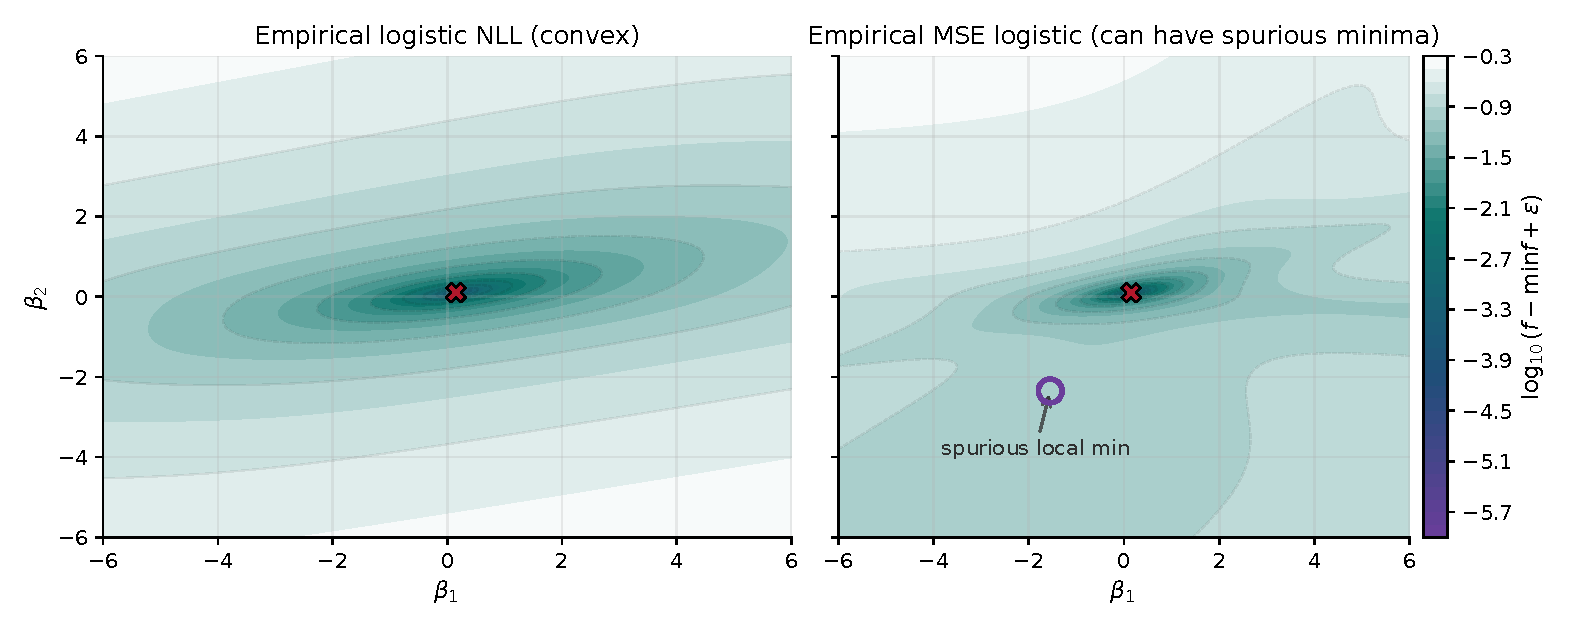
\includegraphics[width=\textwidth]{figures/handouts/convexity_optimization/fig_logistic_empirical_spurious}
  \caption{Empirical logistic landscapes on the dataset in \Cref{ex:logistic-empirical-spurious}.
  The plots show $\log_{10}(f-\min f+\varepsilon)$ for each objective.
  The red X marks the global minimizer in each panel.
  Left: the NLL is convex (one basin).
  Right: the squared-loss objective can have a spurious local minimum (circled), so a local method can get stuck.}
  \label{fig:logistic-empirical-spurious}
\end{figure}

\begin{figure}[t]
  \centering
  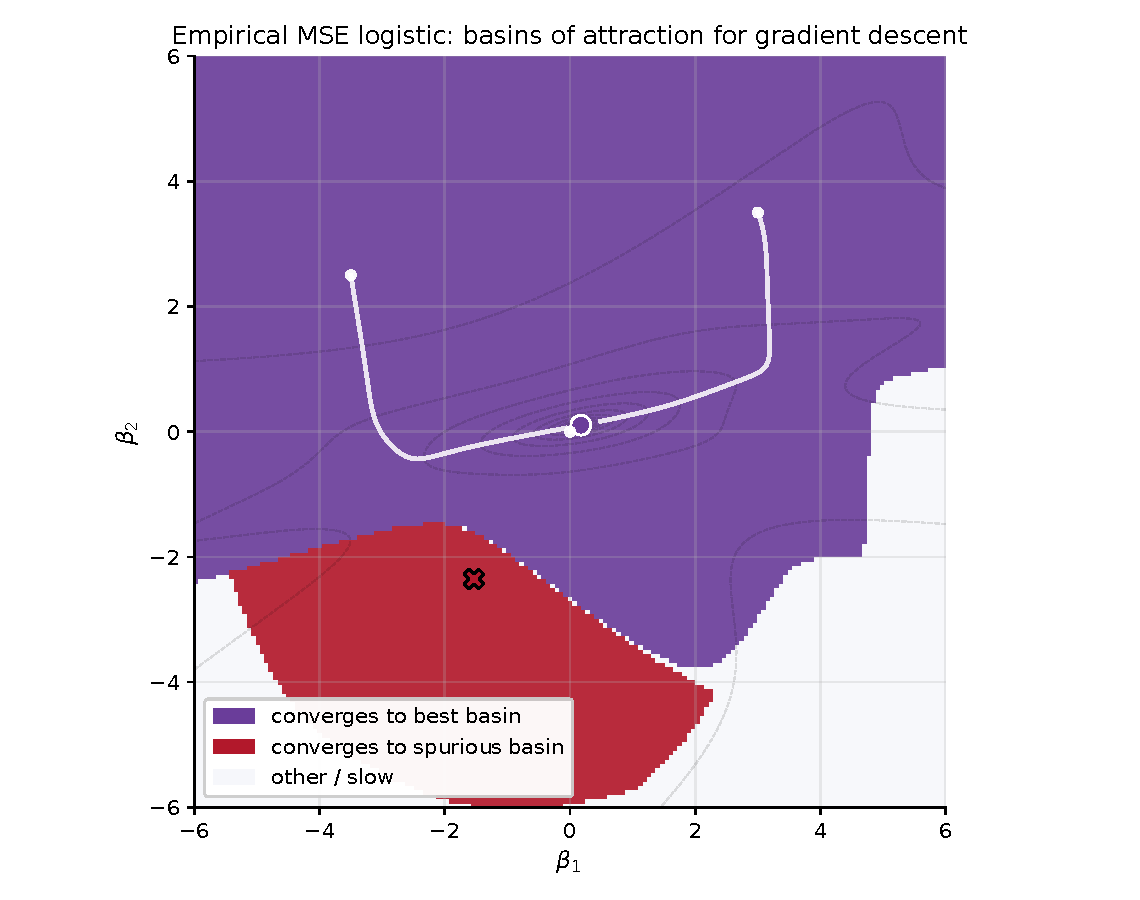
\includegraphics[width=0.92\textwidth]{figures/handouts/convexity_optimization/fig_logistic_empirical_basins}
  \caption{Basins of attraction for gradient descent on the empirical MSE-logistic objective in \Cref{ex:logistic-empirical-spurious}.
  The purple dot and red X mark the two local minimizers.
  Each initialization is colored by which local minimizer fixed-step GD (with $\eta=0.6$) converges to, and the overlaid paths show a few representative trajectories.}
  \label{fig:logistic-empirical-basins}
\end{figure}

Now assume a realizable population model:
\[
Y\mid X=x \sim \mathrm{Bernoulli}(p^\star(x)),
\qquad
p^\star(x) = \sigma(x^\top\beta^\star).
\]
Then the expected squared loss decomposes as
\[
\E\big[(Y-\sigma(X^\top\beta))^2\mid X\big]
= p^\star(X)(1-p^\star(X)) + \big(p^\star(X)-\sigma(X^\top\beta)\big)^2,
\]
so (up to an additive constant) the population objective becomes
\begin{equation}
R(\beta) = \E\big[(\sigma(X^\top\beta)-\sigma(X^\top\beta^\star))^2\big].
\label{eq:logistic-pop-risk}
\end{equation}

\begin{proposition}[One-point monotonicity in the realizable population squared-loss risk]
\label{prop:logistic-pop-one-point}
Assume $\E[\norm{X}_2]<\infty$, and let $R$ be as in \eqref{eq:logistic-pop-risk}. Then for all $\beta$,
\begin{equation}
\ip{\nabla R(\beta)}{\beta-\beta^\star} \ge 0.
\label{eq:one-point}
\end{equation}
In particular, along any ray $\beta(t)=\beta^\star+t(\beta-\beta^\star)$, the function $t\mapsto R(\beta(t))$ is nondecreasing for $t\ge 0$.
\end{proposition}

The next exercise isolates the population monotonicity calculation; structurally it plays the same role as the first-order convexity arguments in the Optimization unit.
\begin{exercise}[One-point monotonicity for realizable MSE-logistic]
\label{ex:logistic-one-point}
Prove \Cref{prop:logistic-pop-one-point}.
Let $\eta=X^\top\beta$ and $\eta^\star=X^\top\beta^\star$.
\begin{enumerate}[leftmargin=*]
  \item Differentiate under the expectation in \eqref{eq:logistic-pop-risk} to show that
  \[
  \nabla R(\beta)
  =2\,\E\Big[(\sigma(\eta)-\sigma(\eta^\star))\,\sigma'(\eta)\,X\Big].
  \]
  \item Show that
  \[
  \ip{\nabla R(\beta)}{\beta-\beta^\star}
  =2\,\E\Big[\sigma'(\eta)\,(\sigma(\eta)-\sigma(\eta^\star))(\eta-\eta^\star)\Big],
  \]
  and conclude it is nonnegative using only that $\sigma$ is increasing and $\sigma'\ge 0$.
  \item Deduce the ray-monotonicity statement by differentiating $g(t)=R(\beta^\star+t(\beta-\beta^\star))$.
\end{enumerate}
\end{exercise}

\SolutionBox[14]{%
\emph{Part (1).}
Differentiate \eqref{eq:logistic-pop-risk} under the expectation:
\[
R(\beta)=\E\big[(\sigma(X^\top\beta)-\sigma(X^\top\beta^\star))^2\big].
\]
Using the chain rule, $\nabla_\beta\sigma(X^\top\beta)=\sigma'(X^\top\beta)\,X$, hence
\[
\nabla R(\beta)
=2\,\E\Big[(\sigma(\eta)-\sigma(\eta^\star))\,\sigma'(\eta)\,X\Big],
\qquad
\eta=X^\top\beta,\ \eta^\star=X^\top\beta^\star.
\]

\emph{Part (2).}
Take the inner product with $(\beta-\beta^\star)$ and use $\ip{X}{\beta-\beta^\star}=\eta-\eta^\star$:
\[
\ip{\nabla R(\beta)}{\beta-\beta^\star}
=2\,\E\Big[\sigma'(\eta)\,(\sigma(\eta)-\sigma(\eta^\star))(\eta-\eta^\star)\Big].
\]
Since $\sigma'(\eta)\ge 0$ and $\sigma$ is increasing, we have
$(\sigma(\eta)-\sigma(\eta^\star))(\eta-\eta^\star)\ge 0$ pointwise.
Therefore the integrand is pointwise nonnegative, and the expectation is nonnegative as claimed.

\emph{Part (3) (ray monotonicity).}
For the ray $\beta(t)=\beta^\star+t(\beta-\beta^\star)$, define $g(t)=R(\beta(t))$.
By the chain rule,
\[
g'(t)=\ip{\nabla R(\beta(t))}{\beta-\beta^\star}\ge 0,
\]
so $t\mapsto R(\beta(t))$ is nondecreasing for $t\ge 0$.
(The argument uses only that the link is increasing with nonnegative derivative, so it holds for any such link function.)%
}

\begin{corollary}[Realizable population MSE-logistic has no spurious local minima]
\label{cor:logistic-pop-no-spurious}
Under the assumptions of \Cref{prop:logistic-pop-one-point}, every local minimizer of the realizable population risk $R$ in \eqref{eq:logistic-pop-risk} is global.
If in addition $\E[XX^\top]\succ 0$, then the unique global minimizer is $\beta^\star$.
\end{corollary}

\begin{exercise}[Stationarity + one-point monotonicity $\Rightarrow$ no spurious local minima]
\label{ex:logistic-one-point-no-spurious}
Prove \Cref{cor:logistic-pop-no-spurious} from \Cref{prop:logistic-pop-one-point}.
\begin{enumerate}[leftmargin=*]
  \item Let $\bar\beta$ be a local minimizer. Since $R$ is differentiable, $\nabla R(\bar\beta)=0$.
  Combine this with \Cref{eq:one-point} to show that
  \[
    0
    = \ip{\nabla R(\bar\beta)}{\bar\beta-\beta^\star}
    = 2\,\E\Big[\sigma'(\bar\eta)\,(\sigma(\bar\eta)-\sigma(\eta^\star))(\bar\eta-\eta^\star)\Big],
  \]
  where $\bar\eta=X^\top\bar\beta$ and $\eta^\star=X^\top\beta^\star$.
  Conclude that $\sigma(X^\top\bar\beta)=\sigma(X^\top\beta^\star)$ almost surely.
  \item Deduce that $R(\bar\beta)=0$, so $\bar\beta$ is a global minimizer.
  \item For uniqueness: show that if $R(\beta)=0$, then $X^\top(\beta-\beta^\star)=0$ almost surely, and deduce $\beta=\beta^\star$ under $\E[XX^\top]\succ 0$.
\end{enumerate}
\end{exercise}

\SolutionBox[14]{%
\emph{Part (1).}
Let $\bar\beta$ be a local minimizer of the differentiable function $R$.
Then $\nabla R(\bar\beta)=0$.
Applying \Cref{prop:logistic-pop-one-point} at $\beta=\bar\beta$ gives
\[
0
= \ip{\nabla R(\bar\beta)}{\bar\beta-\beta^\star}
= 2\,\E\Big[\sigma'(\bar\eta)\,(\sigma(\bar\eta)-\sigma(\eta^\star))(\bar\eta-\eta^\star)\Big],
\qquad \bar\eta=X^\top\bar\beta,\ \eta^\star=X^\top\beta^\star.
\]
The integrand is pointwise nonnegative because $\sigma'(\bar\eta)\ge 0$ and $\sigma$ is increasing, so the expectation can vanish only if the integrand is zero almost surely.
Since $\sigma'(z)>0$ for every finite $z$, this implies
\[
(\sigma(\bar\eta)-\sigma(\eta^\star))(\bar\eta-\eta^\star)=0
\qquad\text{almost surely.}
\]
Because $\sigma$ is strictly increasing, the product above is zero if and only if $\bar\eta=\eta^\star$, equivalently $\sigma(X^\top\bar\beta)=\sigma(X^\top\beta^\star)$ almost surely.

\emph{Part (2).}
If $\sigma(X^\top\bar\beta)=\sigma(X^\top\beta^\star)$ almost surely, then the integrand in \eqref{eq:logistic-pop-risk} vanishes almost surely, so
\[
R(\bar\beta)=\E\big[(\sigma(X^\top\bar\beta)-\sigma(X^\top\beta^\star))^2\big]=0.
\]
Since $R(\beta^\star)=0$ as well, $\bar\beta$ is a global minimizer.

\emph{Part (3) (uniqueness).}
If $R(\beta)=0$, then
\[
\E\big[(\sigma(X^\top\beta)-\sigma(X^\top\beta^\star))^2\big]=0,
\]
so $\sigma(X^\top\beta)=\sigma(X^\top\beta^\star)$ almost surely.
Since $\sigma$ is strictly increasing, this implies $X^\top(\beta-\beta^\star)=0$ almost surely.
Taking expectations yields
$(\beta-\beta^\star)^\top\E[XX^\top](\beta-\beta^\star)=0$.
If $\E[XX^\top]\succ 0$, then the quadratic form is strictly positive unless $\beta=\beta^\star$, so $\beta^\star$ is the unique global minimizer.%
}

The population MSE-logistic risk is nonconvex, but it still has the simple geometry that moving away from $\beta^\star$ does not help along any ray from $\beta^\star$.
This is qualitatively different from objectives like ecological logistic regression (\Cref{sec:ecological-logistic}), where aggregation introduces intrinsic nonconvexity and the landscape can have many distinct basins even under a clean population model.

Even with this benign global geometry, gradient descent can be slow because of saturation and flat plateaus.
The one-point monotonicity in \Cref{prop:logistic-pop-one-point} is a global geometry guarantee, but it is not a rate guarantee.
Far from $\beta^\star$, the squared-loss logistic objective can become very flat because the logistic link saturates:
$\sigma(z)\to 0$ or $1$ and $\sigma'(z)\to 0$ as $|z|\to\infty$.
The squared-loss gradient carries a factor of $\sigma'(X^\top\beta)$, so when the model is very confident (large $|X^\top\beta|$), the gradient can be tiny even if the objective value is not close to its minimum.
This mirrors the ``confidence weights'' story for convex NLL objectives:
in logistic NLL, curvature is largest near the decision boundary, while very confident points contribute little.
For squared loss, that same saturation suppresses the \emph{descent signal} itself, producing plateaus where $\norm{\nabla R(\beta)}_2$ is small even though $R(\beta)-R(\beta^\star)$ is not.

\begin{proposition}[Realizable squared-loss logistic: arbitrarily flat far from $\beta^\star$]
\label{prop:logistic-pop-flat}
Assume $\E[\norm{X}_2]<\infty$ and let $R$ be the realizable population risk \eqref{eq:logistic-pop-risk}.
Define $g(t)=R(t\beta^\star)$ for $t\ge 1$.
Then:
\begin{enumerate}[leftmargin=*]
  \item $g$ is nondecreasing on $[1,\infty)$ and converges to a finite limit $g(\infty)$.
  \item $\lim_{t\to\infty} g'(t)=0$ and $\lim_{t\to\infty}\norm{\nabla R(t\beta^\star)}_2=0$.
  \item If $\Pr(X^\top\beta^\star\neq 0)>0$, then $g(\infty)>0$.
\end{enumerate}
In particular, there are directions along which the landscape becomes arbitrarily flat even though the excess risk stays bounded away from $0$.
\end{proposition}

\emph{Proof idea.} See Exercise~\ref{ex:logistic-plateau}.

\begin{exercise}[Prove the plateau]
\label{ex:logistic-plateau}
In the realizable population model, let $g(t)=R(t\beta^\star)$ for $t\ge 1$.
\begin{enumerate}[leftmargin=*]
  \item Show that
  \[
    g'(t)=2\,\E\big[(\sigma(t\eta^\star)-\sigma(\eta^\star))\,\sigma'(t\eta^\star)\,\eta^\star\big],
    \qquad \eta^\star=X^\top\beta^\star,
  \]
  and conclude that $g$ is nondecreasing (hence $g(t)\to g(\infty)$ since $0\le g(t)\le 1$).
  \item Show that $g'(t)\to 0$ and $\nabla R(t\beta^\star)\to 0$ as $t\to\infty$.
  Interpret this as: \emph{without} a PL/strong-convexity-type condition, small gradient does not imply near-optimality.
  \item Assume $\Pr(\eta^\star\neq 0)>0$.
  Show that $g(\infty)>0$.
\end{enumerate}
\end{exercise}

\SolutionBox[12]{%
Write $\eta^\star=X^\top\beta^\star$ so that $g(t)=\E[(\sigma(t\eta^\star)-\sigma(\eta^\star))^2]$.

\emph{Part (1).}
Differentiate under the expectation:
by the chain rule,
\[
\frac{d}{dt}\sigma(t\eta^\star)=\sigma'(t\eta^\star)\,\eta^\star,
\]
so
\[
g'(t)
=\E\Big[2(\sigma(t\eta^\star)-\sigma(\eta^\star))\cdot \sigma'(t\eta^\star)\,\eta^\star\Big]
=2\,\E\big[(\sigma(t\eta^\star)-\sigma(\eta^\star))\,\sigma'(t\eta^\star)\,\eta^\star\big].
\]
For $t\ge 1$, $\sigma(t\eta^\star)-\sigma(\eta^\star)$ has the same sign as $(t-1)\eta^\star$ since $\sigma$ is increasing.
Because $\sigma'\ge 0$, the integrand is pointwise nonnegative, hence $g'(t)\ge 0$ and $g$ is nondecreasing.
Since $g(t)\in[0,1]$, it follows that $g(t)\to g(\infty)$ for some finite limit $g(\infty)$.

\emph{Part (2).}
For each fixed $\eta^\star\neq 0$, we have $t\eta^\star\to \pm\infty$ and therefore $\sigma'(t\eta^\star)\to 0$ as $t\to\infty$.
Also,
\[
\big|(\sigma(t\eta^\star)-\sigma(\eta^\star))\,\sigma'(t\eta^\star)\,\eta^\star\big|
\le \sigma'(0)\,|\eta^\star|
\le \sigma'(0)\,\norm{\beta^\star}_2\,\norm{X}_2,
\]
which is integrable since $\E[\norm{X}_2]<\infty$.
We will use the following standard fact: if random variables $Z_t$ satisfy $|Z_t|\le W$ with $\E[W]<\infty$ and $Z_t\to 0$ almost surely, then $\E[Z_t]\to 0$.
Applying this fact here gives $g'(t)\to 0$ as $t\to\infty$.

\smallskip
Similarly, differentiating \eqref{eq:logistic-pop-risk} gives
\[
\nabla R(t\beta^\star)
=2\,\E\big[(\sigma(t\eta^\star)-\sigma(\eta^\star))\,\sigma'(t\eta^\star)\,X\big].
\]
The integrand norm is bounded by $2\sigma'(0)\norm{X}_2$, and for each fixed $X$ the factor $\sigma'(t\eta^\star)$ tends to $0$ (or the bracketed term vanishes when $\eta^\star=0$), so the same reasoning lets us pass the limit through the expectation and conclude $\nabla R(t\beta^\star)\to 0$.

\emph{Part (3).}
As $t\to\infty$ we have $\sigma(t\eta^\star)\to 1$ when $\eta^\star>0$, $\sigma(t\eta^\star)\to 0$ when $\eta^\star<0$, and $\sigma(t\eta^\star)=\sigma(\eta^\star)=1/2$ when $\eta^\star=0$.
Since $0\le (\sigma(t\eta^\star)-\sigma(\eta^\star))^2\le 1$, we can apply the same fact (with $W=1$) to pass the limit through the expectation and obtain
\[
g(\infty)=\E\Big[(1-\sigma(\eta^\star))^2\mathbf{1}\{\eta^\star>0\} + \sigma(\eta^\star)^2\mathbf{1}\{\eta^\star<0\}\Big].
\]
If $\Pr(\eta^\star\neq 0)>0$, then the integrand is strictly positive on $\{\eta^\star\neq 0\}$, so $g(\infty)>0$.

Along this ray, the risk can remain bounded away from $0$ while the gradient (and directional derivative) goes to $0$.
Without a condition like PL/strong convexity, a small gradient does not by itself certify near-optimality.
}

Conditions like strong convexity or the PL inequality (\Cref{def:pl-inequality}) prevent this phenomenon: they rule out large flat regions away from the optimum by relating gradient size to suboptimality.
\Cref{prop:logistic-pop-flat} shows the realizable squared-loss logistic risk does not have such a global guarantee in general.

In the realizable population model, the one-point monotonicity in \Cref{prop:logistic-pop-one-point} is a \emph{global} geometric statement.
To get an actual rate for gradient descent, we also need a \emph{local curvature} condition near $\beta^\star$.
One simple sufficient condition is bounded features, which implies local strong convexity (hence a linear rate) around the optimum.

\begin{proposition}[Local linear convergence of gradient descent near $\beta^\star$]
\label{prop:logistic-pop-local-rate}
Assume $\E[XX^\top]\succeq \lambda I_d$ and $\norm{X}_2\le R$ almost surely for some $\lambda,R>0$.
Then at $\beta^\star$,
\[
\Hess R(\beta^\star)\succeq m_0 I_d,
\qquad
m_0 = 2\,\sigma'(R\norm{\beta^\star}_2)^2\,\lambda,
\]
and there exist $r>0$ and constants $0<m\le L<\infty$ such that the population risk $R$ in \eqref{eq:logistic-pop-risk} is $m$-strongly convex and $L$-smooth on the ball $\{\beta:\ \norm{\beta-\beta^\star}_2\le r\}$.
Consequently, gradient descent with step size $1/L$ initialized in this ball satisfies
\[
R(\beta^{(k)})-R(\beta^\star)
\le \left(1-\frac{m}{L}\right)^k\bigl(R(\beta^{(0)})-R(\beta^\star)\bigr)
\qquad\text{(see \citealp[\S9.3]{boyd_vandenberghe_2004_convex}).}
\]
\end{proposition}

\begin{proof}
Differentiate \eqref{eq:logistic-pop-risk} twice.
At $\beta=\beta^\star$, the cross term vanishes and the Hessian simplifies to
\[
\Hess R(\beta^\star)=2\,\E\big[\sigma'(X^\top\beta^\star)^2\,XX^\top\big].
\]
Since $\norm{X^\top\beta^\star}\le \norm{X}_2\norm{\beta^\star}_2\le R\norm{\beta^\star}_2$ almost surely, we have
$\sigma'(X^\top\beta^\star)\ge \sigma'(R\norm{\beta^\star}_2)>0$ almost surely (since $\sigma'$ is even and decreases with $|z|$), hence
\[
\Hess R(\beta^\star)\succeq 2\,\sigma'(R\norm{\beta^\star}_2)^2\,\E[XX^\top]\succeq 2\,\sigma'(R\norm{\beta^\star}_2)^2\,\lambda I_d.
\]
This is the claimed bound with $m_0=2\,\sigma'(R\norm{\beta^\star}_2)^2\,\lambda$.
Because $R$ is twice continuously differentiable and $\norm{X}_2\le R$ almost surely, $\Hess R(\beta)$ varies continuously in $\beta$ and is bounded on compact sets.
Therefore, on a sufficiently small ball around $\beta^\star$, the Hessian is bounded below by (say) $\tfrac12 m_0 I_d$ and above by $L I_d$ for some finite $L$, which gives local strong convexity and smoothness.
The linear convergence rate for gradient descent on an $m$-strongly convex and $L$-smooth function is standard (cited above).
\end{proof}

Under misspecification, hard multimodality can return.
If $p^\star(x)$ is not representable as $\sigma(x^\top\beta)$ (e.g.\ marginalizing over latent classes can yield mixtures of logits), then \eqref{eq:one-point} need not hold, and the population squared-loss risk can become bimodal with spurious local minima.
Benign global geometry often hinges on model and data assumptions.
This is one reason MLE (convex NLL) is often more stable than squared-loss fitting in logistic-type binary regression models.

\begin{example}[Misspecification can create a spurious local minimum for squared-loss logistic regression]
\label{ex:logistic-misspecified-spurious}
Consider a 1D feature $X$ that takes values $\{-2,-1,1,2\}$ with equal probability, and parameterize $\beta=(\beta_0,\beta_1)$ so that $q_\beta(x)=\sigma(\beta_0+\beta_1 x)$.
Let the true conditional probabilities be
\[
p^\star(-2)=0.49,\quad p^\star(-1)=0.87,\quad p^\star(1)=0.92,\quad p^\star(2)=0.36.
\]
This $p^\star$ is not representable as $q_\beta$, since it is not monotone in $x$.

For the population squared-loss risk $R_{\mathrm{MSE}}(\beta)=\E[(q_\beta(X)-p^\star(X))^2]$, a direct evaluation shows two distinct basins:
numerically, evaluating $R_{\mathrm{MSE}}$ on a grid reveals a global minimizer and a spurious local minimizer.
See \Cref{fig:logistic-landscape-2d}.
\end{example}

\begin{figure}[t]
  \centering
  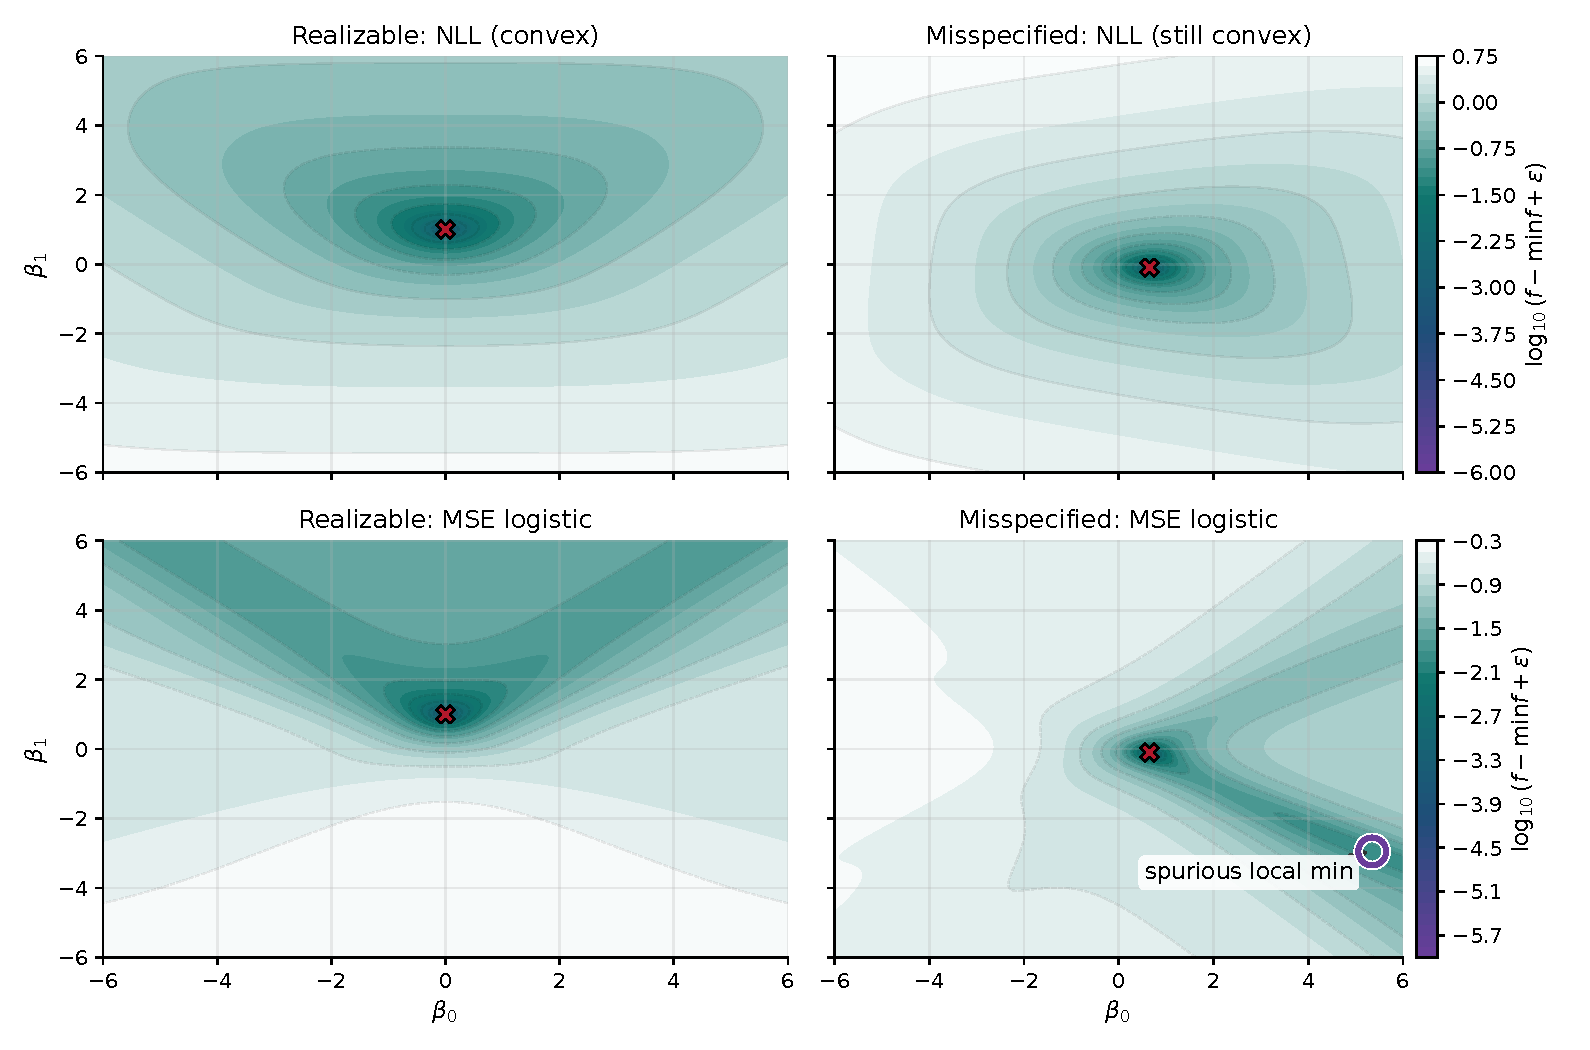
\includegraphics[width=\textwidth]{figures/handouts/convexity_optimization/fig_logistic_landscape_2d}
  \caption{A consistent contourf view of logistic landscapes in a 2D parameterization $\beta=(\beta_0,\beta_1)$.
  The plots show $\log_{10}(f-\min f+\varepsilon)$ for each objective, which makes basins comparable across panels.
  The red X marker indicates the global minimizer in each panel; in the bottom-right plot, the circled point is a spurious local minimum.
  In this example, the NLL landscape is unimodal in both realizable and misspecified settings, while the squared-loss landscape can develop extra basins under misspecification.}
  \label{fig:logistic-landscape-2d}
\end{figure}

% ------------------------------------------------------------
Example~I separates three distinct regimes.
Empirical MSE-logistic can create spurious basins; the realizable population risk has no spurious local minima but can still be slow because of broad plateaus; and misspecification can bring back genuinely wrong stable basins.
The response depends on the regime: use a stable objective when possible, use damping or line search when curvature is unreliable, and use restarts or stronger initializations when multiple basins are present.

% ------------------------------------------------------------
\section[Example II (phase retrieval)]{Example II: multimodality from symmetry, but only global optima in phase retrieval}
\label{sec:phase-retrieval}

In coherent diffraction imaging, optics, and astronomy, sensors measure intensities and lose phase.
A canonical real model is \emph{phase retrieval}:
\[
y_i = (a_i^\top x^\star)^2,\qquad i=1,\dots,m,
\]
where $x^\star\in\R^d$ is the unknown signal and $a_i$ are known sensing vectors.
A standard nonconvex least-squares objective is
\begin{equation}
F(x)=\frac{1}{4m}\sum_{i=1}^m\big((a_i^\top x)^2 - y_i\big)^2.
\label{eq:phase-empirical}
\end{equation}
This objective is nonconvex for structural reasons (it involves squares of linear forms),
and it is \emph{inherently} multimodal because $x^\star$ and $-x^\star$ generate the same data.

Like squared-loss logistic regression, phase retrieval is a smooth, nonconvex least-squares objective.
But here the nonconvexity is driven primarily by a \emph{symmetry}: $x^\star$ and $-x^\star$ generate the same data.
In population (for Gaussian designs), this symmetry produces multiple global optima but \emph{no} suboptimal local minima; the remaining stationary points are saddles.
This is ``benign'' nonconvexity (a strict-saddle picture), and it contrasts with ecological logistic regression (\Cref{sec:ecological-logistic}), where aggregation creates intrinsic nonconvexity and can lead to many distinct basins.
This ``benign geometry'' picture (multiple equivalent global minimizers; strict saddles elsewhere) appears broadly in modern tractable nonconvex problems; see \citet[\S2]{sun_qu_wright_2015_nonconvex_not_scary} and \citet[\S1]{zhang_qu_wright_2020_symmetry_geometry}.

\begin{figure}[t]
  \centering
  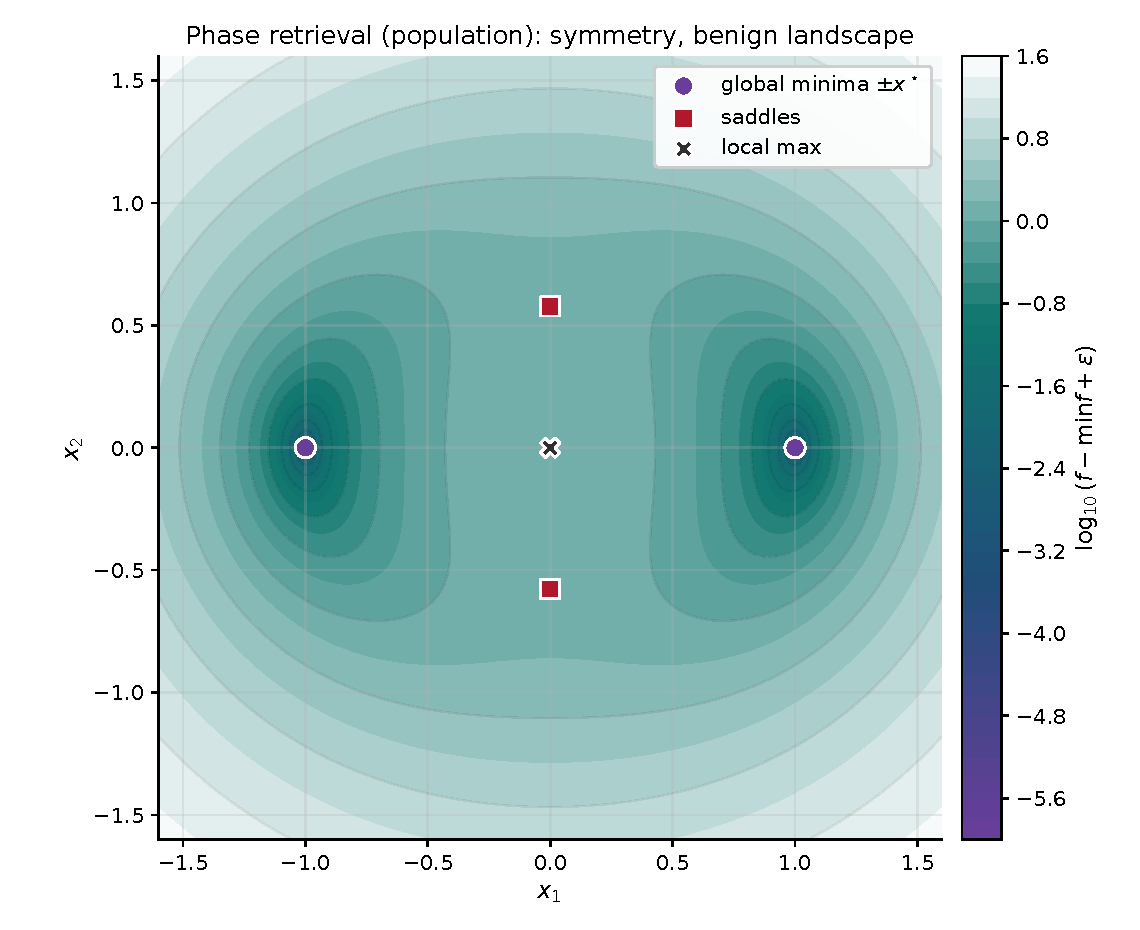
\includegraphics[width=0.86\textwidth]{figures/handouts/convexity_optimization/fig_phase_retrieval_landscape}
  \caption{Population phase retrieval in $d=2$: the landscape is nonconvex and symmetric ($x\sim -x$), but the only local minima are the two global minima $\pm x^\star$; other critical points are saddles or a local maximum at the origin.}
  \label{fig:phase-retrieval-landscape}
\end{figure}

For a clean population model, assume $a\sim N(0,I_d)$ and consider the \emph{population} objective
\begin{equation}
  f(x)=\frac12\,\E\Big[\big((a^\top x)^2 - (a^\top x^\star)^2\big)^2\Big].
  \label{eq:phase-pop}
\end{equation}

\begin{proposition}[Population phase retrieval: nonconvex but no spurious local minima]
\label{prop:phase-retrieval-benign}
For $f$ in \eqref{eq:phase-pop},
\begin{equation}
  f(x)
  =\frac{3}{2}\norm{x}^4 - \norm{x}^2\norm{x^\star}^2 - 2\ip{x}{x^\star}^2 + \frac{3}{2}\norm{x^\star}^4,
  \label{eq:phase-pop-closed-form}
\end{equation}
and the stationary points are:
\begin{enumerate}[leftmargin=*]
  \item global minima $x=\pm x^\star$ (value $0$),
  \item a local maximum at $x=0$,
  \item a saddle set $\{x:\ x\perp x^\star,\ \norm{x}=\norm{x^\star}/\sqrt{3}\}$.
\end{enumerate}
In particular, every local minimum is global.
\end{proposition}

\begin{exercise}[Phase retrieval: derive and classify the population stationary points]
\label{ex:phase-pop-derivation}
Prove \Cref{prop:phase-retrieval-benign}.
\begin{enumerate}[leftmargin=*]
  \item Expand \eqref{eq:phase-pop} and use the Gaussian fourth-moment identities
  \[
  \E[(a^\top u)^4]=3\norm{u}^4,
  \qquad
  \E[(a^\top u)^2(a^\top v)^2]=\norm{u}^2\norm{v}^2 + 2\ip{u}{v}^2,
  \]
  to obtain \eqref{eq:phase-pop-closed-form}.
  \item Differentiate \eqref{eq:phase-pop-closed-form} to get an explicit formula for $\nabla f(x)$.
  \item Solve $\nabla f(x)=0$ by decomposing $x=\alpha x^\star + u$ with $u\perp x^\star$.
  \item Classify the stationary points as global minima, a local maximum, and a saddle set.
\end{enumerate}
\end{exercise}

\SolutionBox[22]{%
\emph{Part (1) (closed form).}
Expanding the square in \eqref{eq:phase-pop} gives
\[
f(x)
=\frac12\,\E\big[(a^\top x)^4\big]
\;-\;\E\big[(a^\top x)^2(a^\top x^\star)^2\big]
\;+\;\frac12\,\E\big[(a^\top x^\star)^4\big].
\]
Apply the stated Gaussian fourth-moment identities with $u=x$ and $v=x^\star$ to get
\[
\E[(a^\top x)^4]=3\norm{x}^4,\qquad
\E[(a^\top x^\star)^4]=3\norm{x^\star}^4,
\]
and
\[
\E[(a^\top x)^2(a^\top x^\star)^2]=\norm{x}^2\norm{x^\star}^2 + 2\ip{x}{x^\star}^2.
\]
Substituting yields \eqref{eq:phase-pop-closed-form}.

\emph{Part (2) (gradient).}
Differentiate \eqref{eq:phase-pop-closed-form}:
\[
\nabla f(x)
= 6\norm{x}^2 x - 2\norm{x^\star}^2 x - 4\ip{x}{x^\star}x^\star
= (6\norm{x}^2-2\norm{x^\star}^2)x - 4\ip{x}{x^\star}x^\star.
\]

\emph{Part (3) (stationary points).}
Let $r=\norm{x^\star}_2$ and decompose $x=\alpha x^\star + u$ with $u\perp x^\star$.
Then $\ip{x}{x^\star}=\alpha r^2$ and $\norm{x}^2=\alpha^2r^2+\norm{u}^2$.
Setting $\nabla f(x)=0$ and matching the $u$ and $x^\star$ components gives
\[
(6\norm{x}^2-2r^2)\,u=0,
\qquad
\alpha\,(6\norm{x}^2-6r^2)=0.
\]
If $u=0$, then either $\alpha=0$ (so $x=0$) or $\norm{x}^2=r^2$ (so $\alpha=\pm 1$ and $x=\pm x^\star$).
If $u\neq 0$, then the first equation forces $\norm{x}^2=r^2/3$, and the second forces $\alpha=0$, hence
$x\perp x^\star$ and $\norm{x}=r/\sqrt{3}$.
This gives exactly the stationary-point list in \Cref{prop:phase-retrieval-benign}.

\emph{Part (4) (classification).}
Since $f$ in \eqref{eq:phase-pop} is an expectation of a square, $f(x)\ge 0$ for all $x$.
Also $f(\pm x^\star)=0$, so $\pm x^\star$ are global minima.

For $x=0$, the expansion \eqref{eq:phase-pop-closed-form} shows
\[
f(0)-f(x)= r^2\norm{x}^2 + 2\ip{x}{x^\star}^2 - \frac{3}{2}\norm{x}^4,
\]
which is strictly positive for all sufficiently small $x\neq 0$ (the quadratic term dominates), so $x=0$ is a local maximum.

Finally, if $x\perp x^\star$ and $\norm{x}=r/\sqrt{3}$, then the univariate restriction $t\mapsto f(x+t x^\star)$ has negative second derivative at $t=0$, so there is a direction of negative curvature.
Hence these points are saddles, and every local minimum is global.%
}

This is symmetry-driven nonconvexity with a strict-saddle geometry:
every non-optimal stationary point has a direction of negative curvature.

Phase retrieval is typically approached via the two-stage template in \Cref{alg:two-stage-template}:
use a cheap global initializer, then run a local method.
In the Gaussian model, there is a clean way to build a provably good direction estimate from a simple moment identity.
Assume the noiseless Gaussian design model $a_i \stackrel{\mathrm{iid}}{\sim} N(0,I_d)$ with measurements $y_i=(a_i^\top x^\star)^2$.
Define the \emph{spectral matrix}
\[
  Y = \frac{1}{m}\sum_{i=1}^m y_i a_i a_i^\top.
\]
Also define the radius estimate
\[
  \hat r^2 = \frac{1}{m}\sum_{i=1}^m y_i,
\]
which satisfies $\E[\hat r^2]=\norm{x^\star}_2^2$.
If $\hat u$ is a unit-norm top eigenvector of $Y$, then the standard spectral initializer is $x^{(0)}=\hat r\,\hat u$.

The next proposition explains why this initialization is reasonable.
It shows that (i) the population matrix $\E[Y]$ has a unique leading eigenvector in the $x^\star$ direction, and (ii) if the empirical $Y$ is close to $\E[Y]$ in operator norm then its leading eigenvector must be close to $\pm x^\star/\norm{x^\star}_2$.
(Here $\norm{M}_{\mathrm{op}}$ denotes the operator norm, i.e.\ the largest absolute eigenvalue for a symmetric matrix $M$.)

\begin{proposition}[Gaussian phase retrieval: why the spectral initializer points at $x^\star$]
\label{prop:phase-spectral-init}
Assume $x^\star\neq 0$, let $a\sim N(0,I_d)$, and set $y=(a^\top x^\star)^2$.
Write $r=\norm{x^\star}_2$ and $u^\star=x^\star/r$.
Define the population matrix
\[
  Y_{\mathrm{pop}} = \E\big[y\,a a^\top\big]
  = \E\big[(a^\top x^\star)^2 a a^\top\big].
\]
Then
\[
  Y_{\mathrm{pop}}=r^2 I_d + 2x^\star(x^\star)^\top,
\]
so the unique leading eigenvector of $Y_{\mathrm{pop}}$ is $u^\star$.
Moreover, if $Y$ is any symmetric matrix satisfying
\[
\norm{Y-Y_{\mathrm{pop}}}_{\mathrm{op}} \le \varepsilon\, r^2
\qquad\text{for some }\varepsilon\in(0,1),
\]
then for every unit-norm leading eigenvector $\hat u$ of $Y$ there exists a sign $s\in\{\pm 1\}$ such that
$\norm{\hat u-su^\star}_2\le \sqrt{2\varepsilon}$.
\end{proposition}

\begin{exercise}[Phase retrieval: why spectral initialization points at $x^\star$]
\label{ex:phase-spectral-spike}
Prove \Cref{prop:phase-spectral-init}.
Conclude that if the empirical matrix $Y$ is close to $Y_{\mathrm{pop}}$ in operator norm, then its top eigenvector is close to $\pm u^\star$ and the spectral initializer $x^{(0)}=\hat r\,\hat u$ is close to $\pm x^\star$.
\emph{Hint:} to compute $Y_{\mathrm{pop}}$, you can either compute entries using the Gaussian fourth-moment identity
$\E[a_i a_j a_k a_\ell]=\delta_{ij}\delta_{k\ell}+\delta_{ik}\delta_{j\ell}+\delta_{i\ell}\delta_{jk}$,
or compute the entries directly by expanding.
For the perturbation bound, compare quadratic forms $v^\top Y v$ and use $|v^\top (Y-Y_{\mathrm{pop}}) v|\le \norm{Y-Y_{\mathrm{pop}}}_{\mathrm{op}}$ for unit $v$.
Finally, explain in a sentence why one expects $\norm{Y-Y_{\mathrm{pop}}}_{\mathrm{op}}$ to be small when $m$ is large in the Gaussian model.
\end{exercise}

\SolutionBox[20]{%
Write $u=x^\star$ and expand $y=(a^\top u)^2=\sum_{k,\ell} u_k u_\ell a_k a_\ell$.
For each entry $(i,j)$,
\[
\E\!\big[y\,a_i a_j\big]
=\sum_{k,\ell} u_k u_\ell\,\E[a_i a_j a_k a_\ell]
=\sum_{k,\ell} u_k u_\ell\bigl(\delta_{ij}\delta_{k\ell}+\delta_{ik}\delta_{j\ell}+\delta_{i\ell}\delta_{jk}\bigr).
\]
The first term gives $\delta_{ij}\sum_k u_k^2=\delta_{ij}\norm{u}_2^2$.
The second and third terms each give $u_i u_j$.
Thus $\E[y\,a_i a_j]=\norm{u}_2^2\,\delta_{ij}+2u_i u_j$, i.e.
$Y_{\mathrm{pop}}=\norm{u}_2^2 I_d + 2uu^\top$.

For eigenvalues, note that $Y_{\mathrm{pop}}u=(\norm{u}_2^2+2\norm{u}_2^2)u=3\norm{u}_2^2 u$.
If $w\perp u$, then $uu^\top w=0$ so $Y_{\mathrm{pop}}w=\norm{u}_2^2 w$.
Hence the unique top eigenspace is $\mathrm{span}\{u\}$.

Let $r=\norm{u}_2$ and $u^\star=u/r$.
Let $\hat u$ be a unit top eigenvector of $Y$.
Write $E=Y-Y_{\mathrm{pop}}$ and assume $\norm{E}_{\mathrm{op}}\le \varepsilon r^2$.
Then
\[
\hat u^\top Y_{\mathrm{pop}} \hat u
= \hat u^\top Y \hat u - \hat u^\top E \hat u
\ge \lambda_{\max}(Y) - \norm{E}_{\mathrm{op}}
\ge (u^\star)^\top Y u^\star - \norm{E}_{\mathrm{op}}
\ge 3r^2 - 2\varepsilon r^2.
\]
On the other hand,
$
\hat u^\top Y_{\mathrm{pop}} \hat u
= r^2 + 2r^2\,|\ip{\hat u}{u^\star}|^2.
$
Combining gives $|\ip{\hat u}{u^\star}|^2\ge 1-\varepsilon$.
Choosing the sign that maximizes the inner product,
\[
\min\{\norm{\hat u-u^\star}_2,\norm{\hat u+u^\star}_2\}^2
=2\bigl(1-|\ip{\hat u}{u^\star}|\bigr)
\le 2\bigl(1-|\ip{\hat u}{u^\star}|^2\bigr)
\le 2\varepsilon.
\]

The matrix $Y$ is an empirical average of i.i.d.\ symmetric matrices with mean $Y_{\mathrm{pop}}$.
To make this quantitative in high dimensions, one uses concentration inequalities for random matrices to bound $\norm{Y-Y_{\mathrm{pop}}}_{\mathrm{op}}$ with high probability; see \citet[\S2.2]{zhang_qu_wright_2020_symmetry_geometry} for discussion and references.
These probability tools are largely orthogonal to our focus here.%
}

Once you have an initialization that is close to $\pm x^\star$, the local stage behaves like the convex story again.
In the Gaussian population objective, $\pm x^\star$ are not only global minima: they are \emph{locally strongly convex} minima, so the standard local strong-convexity analysis from the Optimization unit gives a linear rate while the iterates remain in that neighborhood.

\begin{exercise}[Phase retrieval: local convexity near $\pm x^\star$ in the population objective]
\label{ex:phase-pop-local-strong-convex}
For the population objective $f$ in \eqref{eq:phase-pop-closed-form}, compute the Hessian $\Hess f(x)$ and show that
\[
\Hess f(x^\star)=4\norm{x^\star}_2^2 I_d + 8x^\star(x^\star)^\top.
\]
Deduce the eigenvalues of $\Hess f(x^\star)$ and interpret this as a local condition-number statement near $x^\star$.
\end{exercise}

\SolutionBox[12]{%
Differentiate the gradient formula in the solution to \Cref{ex:phase-pop-derivation}:
for $x\in\R^d$,
\[
\Hess f(x)=12xx^\top + (6\norm{x}_2^2-2\norm{x^\star}_2^2)I_d - 4x^\star(x^\star)^\top.
\]
At $x=x^\star$ this becomes
\[
\Hess f(x^\star)=(12-4)x^\star(x^\star)^\top + 4\norm{x^\star}_2^2 I_d
=8x^\star(x^\star)^\top + 4\norm{x^\star}_2^2 I_d.
\]
Along $u^\star=x^\star/\norm{x^\star}_2$ the eigenvalue is $12\norm{x^\star}_2^2$, and along any direction orthogonal to $x^\star$ the eigenvalue is $4\norm{x^\star}_2^2$.
So near $x^\star$ the population objective is well conditioned (local condition number $3$), which is exactly the regime where local methods behave like in the convex case.%
}

These pieces give the standard Gaussian-model story:
spectral initialization supplies a direction close to $\pm x^\star$, and the local geometry near $\pm x^\star$ is strongly convex, so local methods converge quickly once initialized there.
Rigorous finite-sample analyses follow this template; see \citet[\S2.2]{zhang_qu_wright_2020_symmetry_geometry} and references therein.

Phase retrieval shows a different kind of nonconvexity.
The sign symmetry creates multiple optima, but they are equivalent, and the remaining stationary points are saddles rather than bad local minima.
The right response is therefore not exhaustive global search; it is a coarse initializer, such as a spectral method, followed by local refinement inside the basin of $\pm x^\star$.



% ------------------------------------------------------------
\section[Example III (ecological logistic)]{Example III: hard nonconvexity from aggregation in ecological logistic regression}
\label{sec:ecological-logistic}

In some applications we observe covariates at the unit level but only aggregated outcomes.
For example, we might see covariates $x_{g,1},\dots,x_{g,n_g}$ for individuals in a group (a precinct, a cohort, a batch),
but instead of observing the binary outcomes $Y_{g,i}\in\{0,1\}$ we only observe the group total
\[
Z_g = \sum_{i=1}^{n_g} Y_{g,i}.
\]
Many different binary vectors $(Y_{g,1},\dots,Y_{g,n_g})$ can produce the same total $Z_g$, so the likelihood for $\beta$ must marginalize over a large discrete set of latent ``assignments.''

Assume a logistic model at the unit level:
\[
\Pr(Y_{g,i}=1\mid x_{g,i},\beta)=\sigma(x_{g,i}^\top\beta),
\qquad i=1,\dots,n_g,
\]
with conditional independence across $i$ given the covariates.
Write $p_{g,i}(\beta)=\sigma(x_{g,i}^\top\beta)$.
Then $Z_g$ is a sum of independent but non-identically distributed Bernoulli random variables (a Poisson--binomial model), and the marginal likelihood contains $\binom{n_g}{z_g}$ terms.
The resulting negative log-likelihood is typically nonconvex in $\beta$.
This combinatorial marginalization also creates a separate difficulty that is easy to miss if we focus only on the geometry:
when $n_g$ is large, the likelihood term $\Pr(Z_g=z_g\mid x_{g,1},\dots,x_{g,n_g},\beta)$ can be expensive to evaluate repeatedly inside an optimizer.
The naive computation is literally a sum over $\binom{n_g}{z_g}$ assignments (as in \Cref{ex:eco-logistic-nonconvex}), which is intractable for large groups.
This ``optimization + marginalization'' pattern is common in latent-variable models: hard landscapes and expensive objective evaluations can come together.

An empirical negative log-likelihood objective for $G$ independent groups is
\begin{equation}
  f(\beta)
  =
  -\frac{1}{G}\sum_{g=1}^G \log \Pr(Z_g=z_g \mid x_{g,1},\dots,x_{g,n_g},\beta).
  \label{eq:eco-logistic-obj}
\end{equation}
Two edge cases are instructive.
In the special case where the covariates are constant within each group ($x_{g,i}\equiv x_g$), we have
$Z_g\sim \mathrm{Binomial}(n_g,\sigma(x_g^\top\beta))$, and \eqref{eq:eco-logistic-obj} reduces to the usual convex binomial logistic-regression objective from the Optimization unit.
At the other extreme, if $d=1$ with $\beta=(\beta_0,\beta_1)$ and each group contains covariates in $\pm$ pairs (for every $x$ the value $-x$ appears with the same multiplicity), then the marginal likelihood is symmetric in the slope: it is unchanged under $\beta_1\mapsto -\beta_1$.
This kind of symmetry reflects a genuine non-identifiability from totals alone.

\begin{exercise}[Ecological logistic regression: two easy special cases]
\label{ex:eco-logistic-edge-cases}
\begin{enumerate}[leftmargin=*]
  \item Suppose $x_{g,i}\equiv x_g$ within each group.
  Show that $Z_g\sim \mathrm{Binomial}(n_g,\sigma(x_g^\top\beta))$ and conclude that the corresponding negative log-likelihood is convex in $\beta$.
  \item Assume $d=1$ with $\beta=(\beta_0,\beta_1)$ and suppose the multiset $\{x_1,\dots,x_n\}$ is symmetric: for every $x$ it contains $-x$ with the same multiplicity.
  Show that, for every $z$,
  \[
    \Pr(Z=z\mid x_1,\dots,x_n,(\beta_0,\beta_1))
    =
    \Pr(Z=z\mid x_1,\dots,x_n,(\beta_0,-\beta_1)).
  \]
  Conclude that the likelihood for $\beta_1$ is an even function, so the sign of the slope is not identifiable from $Z$ alone in such a balanced design.
\end{enumerate}
\end{exercise}

\SolutionBox[14]{%
\emph{Part (1).}
If $x_{g,i}\equiv x_g$, then conditional on $x_g$ the unit-level outcomes are i.i.d.\ Bernoulli with success probability $\sigma(x_g^\top\beta)$.
Therefore $Z_g=\sum_{i=1}^{n_g}Y_{g,i}\sim \mathrm{Binomial}(n_g,\sigma(x_g^\top\beta))$.
Up to an additive constant (independent of $\beta$), the per-group negative log-likelihood can be written as a function of the scalar $\eta=x_g^\top\beta$:
\[
\ell_g(\beta)
= -z_g\,\eta + n_g\log(1+e^\eta).
\]
Since $\frac{d^2}{d\eta^2}\ell_g(\eta)=n_g\,\sigma'(\eta)\ge 0$, the map $\eta\mapsto \ell_g(\eta)$ is convex.
Composing a convex function with a linear map $\beta\mapsto x_g^\top\beta$ preserves convexity, so $\ell_g$ is convex in $\beta$.
Summing over $g$ preserves convexity, hence the full objective is convex.

\emph{Part (2).}
Write $p_i(\beta_0,\beta_1)=\sigma(\beta_0+\beta_1 x_i)$.
Replacing $\beta_1$ by $-\beta_1$ replaces $p_i$ by $\tilde p_i=\sigma(\beta_0-\beta_1 x_i)$.
By the assumed symmetry of the multiset $\{x_i\}$, the multiset $\{\tilde p_i\}$ is the same as $\{p_i\}$ up to a permutation (each $x$ is paired with $-x$).
But the distribution of $Z=\sum_i Y_i$ depends only on the multiset of success probabilities, not on how they are ordered, so $\Pr(Z=z\mid x_1,\dots,x_n,(\beta_0,\beta_1))=\Pr(Z=z\mid x_1,\dots,x_n,(\beta_0,-\beta_1))$ for every $z$.
Thus the likelihood is an even function of $\beta_1$, which means the sign of the slope is not identifiable from totals in this balanced design.%
}

This example ties directly to the empirical-versus-population theme from Example~I.
There the bad basins can be a finite-sample artifact under benign population geometry; here the nonconvexity is intrinsic, because even under the correct model and infinite data aggregation forces us to marginalize over discrete latent assignments.
That marginalization step is also the bridge to the Expectation--maximization subsection of the Augmented-state optimization unit: once the assignments are latent, the natural algorithmic object is the EM update map, which alternates exact conditional expectations with parameter updates, rather than a single closed-form convex objective.

To emphasize this, it is useful to look at a \emph{population} version of \eqref{eq:eco-logistic-obj}.
Let $X=(x_1,\dots,x_n)$ denote a random group of covariates and let $Z$ be generated from the model under a true parameter $\beta^\star$.
Define the population objective
\[
F(\beta)=\E\big[-\log \Pr(Z\mid X,\beta)\big].
\]
Because the model is correctly specified, $F$ is minimized at (an observationally equivalent version of) $\beta^\star$.
However, as \Cref{fig:eco-logistic-pop-landscape} illustrates, $F$ can still have multiple separated basins and spurious local minima.

\begin{figure}[H]
  \centering
  \input{figures/handouts/convexity_optimization/fig_ecological_logistic_population_landscape}
  \caption{A toy \emph{population} objective for ecological logistic regression in a 2D parameterization $\beta=(\beta_0,\beta_1)$.
  Each group has $n=6$ units and is equally likely to have covariates $(-4,-3,-2,2,3,4)$, $(-3,-1,1,2,3,4)$, or $(-2,-1,1,2,3,4)$ (in $d=1$); outcomes are generated under $\beta^\star=(0.3,1.2)$.
  The plot shows $\log_{10}(F-\min F+\varepsilon)$, as in \Cref{fig:logistic-landscape-2d}; the red X marks $\beta^\star$ and the open circles mark three spurious local minima in this toy example.}
  \label{fig:eco-logistic-pop-landscape}
\end{figure}

\begin{exercise}[Ecological logistic regression: marginalization and nonconvexity]
\label{ex:eco-logistic-nonconvex}
Fix one group with covariates $x_1,\dots,x_n\in\R^d$ and observe $Z=z$.
Let $p_i(\beta)=\sigma(x_i^\top\beta)$.
\begin{enumerate}[leftmargin=*]
  \item Show that
  \[
    \Pr(Z=z\mid x_1,\dots,x_n,\beta)
    =
    \sum_{\substack{S\subseteq\{1,\dots,n\}\\|S|=z}}
    \ \prod_{i\in S} p_i(\beta)\prod_{j\notin S}\bigl(1-p_j(\beta)\bigr).
  \]
  Interpret this as summing over all ways to choose which $z$ units are the successes.
  \item Specialize to $n=2$ and $z=1$ in $d=1$ with covariates $x_1=a$ and $x_2=b$.
  Let $\ell(\beta)$ be the negative log-likelihood $-\log \Pr(Z=1\mid a,b,\beta)$ with no regularization.
  Show that $\ell''(0)=\tfrac12 ab$.
  Conclude that $\ell$ is not convex whenever $ab<0$.
\end{enumerate}
\end{exercise}

\SolutionBox[20]{%
\emph{Part (1).}
Condition on the covariates.
For any binary vector $y=(y_1,\dots,y_n)\in\{0,1\}^n$, conditional independence gives
\[
\Pr(Y_1=y_1,\dots,Y_n=y_n\mid x_1,\dots,x_n,\beta)
=
\prod_{i=1}^n p_i(\beta)^{y_i}\bigl(1-p_i(\beta)\bigr)^{1-y_i}.
\]
The event $\{Z=z\}$ is the union of all assignments $y$ with exactly $z$ ones, so summing over those assignments yields
\[
\Pr(Z=z\mid x_1,\dots,x_n,\beta)
=
\sum_{\substack{y\in\{0,1\}^n\\ \sum_i y_i=z}}
\ \prod_{i=1}^n p_i(\beta)^{y_i}\bigl(1-p_i(\beta)\bigr)^{1-y_i}.
\]
Reindexing the sum by the subset $S=\{i:\ y_i=1\}$ (which has $|S|=z$) gives the stated formula.

\emph{Part (2).}
For $n=2$ and $z=1$, let $p_1(\beta)=\sigma(a\beta)$ and $p_2(\beta)=\sigma(b\beta)$.
Then
\[
q(\beta)=\Pr(Z=1\mid a,b,\beta)
 = p_1(1-p_2) + (1-p_1)p_2
 = p_1+p_2-2p_1p_2,
\]
and $\ell(\beta)=-\log q(\beta)$.
At $\beta=0$ we have $p_1=p_2=\tfrac12$, so $q(0)=\tfrac12$.
Also $p_1'(\beta)=a\,p_1(1-p_1)$ and $p_2'(\beta)=b\,p_2(1-p_2)$, so $p_1'(0)=a/4$ and $p_2'(0)=b/4$.
A direct differentiation gives $q'(0)=0$ and
\[
q''(0)=-4p_1'(0)p_2'(0)=-4\cdot\frac{a}{4}\cdot\frac{b}{4}=-\frac{ab}{4}.
\]
Since $\ell'=-q'/q$ and $q'(0)=0$, we have $\ell''(0)=-(q''(0)/q(0))$ and therefore
\[
\ell''(0)
=-\frac{q''(0)}{q(0)}
=-\frac{-ab/4}{1/2}
=\frac{ab}{2}.
\]
If $ab<0$, then $\ell''(0)<0$, so $\ell$ is not convex.
}

Even though the landscape can be globally hard (and even the population objective can have spurious basins, as in \Cref{fig:eco-logistic-pop-landscape}), there is still a familiar ``convex'' story \emph{locally} around the true parameter under correct specification.
When the model is locally identifiable, the population objective has a neighborhood of $\beta^\star$ on which it is convex (indeed strongly convex).
One convenient way to see this in ecological logistic regression is to expose the probabilistic structure behind the gradient and Hessian: the observed-data objective involves marginalizing over latent assignments, and its Hessian can be written as a difference of two covariance matrices.
After averaging over the random total $Z$ under the true model, that difference becomes a covariance by the law of total covariance.

\begin{exercise}[Ecological logistic regression: DC structure and local convexity near $\beta^\star$]
\label{ex:eco-logistic-pop-local-convex}
Fix covariates $x_1,\dots,x_n\in\R^d$.
For $\beta\in\R^d$, let $V_1,\dots,V_n$ be independent Bernoulli random variables with
\[
\Pr(V_j=1\mid x_j,\beta)=\sigma(x_j^\top\beta),
\qquad j=1,\dots,n,
\]
and define
\[
U = \sum_{j=1}^n x_j V_j,
\qquad
Z = \sum_{j=1}^n V_j.
\]
For an observed total $Z=z$, write $L_z(\beta)=-\log \Pr(Z=z\mid x_1,\dots,x_n,\beta)$.
\begin{enumerate}[leftmargin=*]
  \item Show the \emph{difference-of-convex (DC)} form
  \[
  L_z(\beta)
  =\sum_{j=1}^n \log\bigl(1+e^{x_j^\top\beta}\bigr)
  -\log\left(\sum_{\substack{S\subseteq\{1,\dots,n\}\\|S|=z}} \exp\Big(\sum_{j\in S} x_j^\top\beta\Big)\right).
  \]
  \item Show that $\nabla L_z(\beta)=\E[U]-\E[U\mid Z=z]$.
  \item Show that $\Hess L_z(\beta)=\mathrm{Cov}(U)-\mathrm{Cov}(U\mid Z=z)$.
  (Hint: for $g(\beta)=\log\sum_k e^{a_k^\top\beta}$, the Hessian is the covariance of the vectors $\{a_k\}$ under the corresponding softmax weights.)
  \item Consider the population objective $F(\beta)=\E[L_Z(\beta)]$ when $Z$ is generated under a true parameter $\beta^\star$.
  Assuming the outer expectation defining $F$ can be differentiated twice under the integral sign, use the conditional law of total covariance,
  \[
    \mathrm{Cov}(U\mid X)=\E[\mathrm{Cov}(U\mid Z,X)\mid X] + \mathrm{Cov}(\E[U\mid Z,X]\mid X),
  \]
  to show that
  \[
    \E\big[\Hess L_Z(\beta^\star)\mid X\big]
    = \mathrm{Cov}\big(\E[U\mid Z,X]\mid X\big)\succeq 0.
  \]
  Deduce that
  \[
    \Hess F(\beta^\star)
    = \E\Big[\mathrm{Cov}\big(\E[U\mid Z,X]\mid X\big)\Big]\succeq 0.
  \]
  Conclude that if $\Hess F(\beta^\star)\succ 0$, then $F$ is locally strongly convex on a neighborhood of $\beta^\star$.
\end{enumerate}
\end{exercise}

\SolutionBox[22]{%
\emph{Part (1).}
Write $\eta_j=x_j^\top\beta$ and $p_j=\sigma(\eta_j)=e^{\eta_j}/(1+e^{\eta_j})$.
For any subset $S$ with $|S|=z$,
\[
\Pr(V_j=1\ \forall j\in S,\ V_j=0\ \forall j\notin S\mid x_1,\dots,x_n,\beta)
=\prod_{j\in S}p_j\prod_{j\notin S}(1-p_j)
=\frac{\exp(\sum_{j\in S}\eta_j)}{\prod_{j=1}^n(1+e^{\eta_j})}.
\]
Summing over all $S$ with $|S|=z$ gives
\[
\Pr(Z=z\mid x_1,\dots,x_n,\beta)
=\frac{\sum_{|S|=z}\exp(\sum_{j\in S}\eta_j)}{\prod_{j=1}^n(1+e^{\eta_j})}.
\]
Taking $-\log$ yields the stated DC representation.

\emph{Parts (2) and (3).}
The first term in $L_z$ has gradient $\sum_j \sigma(\eta_j)x_j$ and Hessian $\sum_j \sigma'(\eta_j)x_jx_j^\top$.
Since $U=\sum_j x_j V_j$ with independent Bernoulli coordinates, these are exactly $\E[U]$ and $\mathrm{Cov}(U)$.

For the second term, define a probability distribution on subsets $S$ of size $z$ by
\[
w_S(\beta)\propto \exp\Big(\sum_{j\in S}x_j^\top\beta\Big),
\qquad |S|=z.
\]
This is the conditional law of the success set $\{j:\ V_j=1\}$ given $Z=z$ under parameter $\beta$.
Therefore
\[
\nabla \log\Big(\sum_{|S|=z} e^{\sum_{j\in S}x_j^\top\beta}\Big)
  = \sum_{|S|=z} w_S(\beta)\sum_{j\in S}x_j
  = \E[U\mid Z=z],
\]
and differentiating once more gives
\[
\Hess\!\left(\log\Big(\sum_{|S|=z} e^{\sum_{j\in S}x_j^\top\beta}\Big)\right)
=\mathrm{Cov}(U\mid Z=z),
\]
which yields $\nabla L_z=\E[U]-\E[U\mid Z=z]$ and $\Hess L_z=\mathrm{Cov}(U)-\mathrm{Cov}(U\mid Z=z)$.

\emph{Part (4).}
Now let $X=(x_1,\dots,x_n)$ be random, and assume we may differentiate the outer expectation in $F(\beta)=\E[L_Z(\beta)]$ twice under the integral sign.
Conditional on $X$ and at $\beta^\star$, take expectations over $Z$:
\[
\E\big[\Hess L_Z(\beta^\star)\mid X\big]
=\mathrm{Cov}(U\mid X)-\E[\mathrm{Cov}(U\mid Z,X)\mid X].
\]
By the conditional law of total covariance,
\[
\mathrm{Cov}(U\mid X)
=\E[\mathrm{Cov}(U\mid Z,X)\mid X] + \mathrm{Cov}(\E[U\mid Z,X]\mid X),
\]
so the difference is
\[
\E\big[\Hess L_Z(\beta^\star)\mid X\big]
=\mathrm{Cov}(\E[U\mid Z,X]\mid X)\succeq 0.
\]
Taking outer expectations gives
\[
\Hess F(\beta^\star)
=\E\big[\Hess L_Z(\beta^\star)\big]
=\E\Big[\mathrm{Cov}(\E[U\mid Z,X]\mid X)\Big]\succeq 0.
\]
If this unconditional Hessian is positive definite, then by continuity of $\Hess F$ there exists a radius $r>0$ such that $\Hess F(\beta)\succeq \tfrac12 \Hess F(\beta^\star)\succ 0$ on $\{\beta:\ \norm{\beta-\beta^\star}_2\le r\}$, which implies local strong convexity of $F$ on that neighborhood.%
}

This example still fits the two-stage template in \Cref{alg:two-stage-template}, but the coarse stage is less structured.
In practice, one often uses multiple random starts or a warm start from a crude convex surrogate, then runs a local optimizer with line search or damping on the true nonconvex objective \eqref{eq:eco-logistic-obj} and keeps the best solution found.

Ecological logistic regression is the genuinely hard case in this note.
Aggregation forces a sum over latent assignments, so the objective can have many distinct basins even under correct specification.
The practical response is usually robust search rather than a single clever local method: several starts, warm starts from crude convex surrogates when available, and then local refinement with damping or line search on the true objective.



% ------------------------------------------------------------
\section{Diagnosing nonconvex objectives}
\label{sec:checklist-streamlined}

``Nonconvex'' is not a single regime.
Squared-loss logistic regression is close to convex: the empirical objective can have spurious minima, yet under realizability the population geometry is benign and locally strongly convex near $\beta^\star$.
Phase retrieval is symmetry-driven: there can be multiple equivalent optima but no bad local minima.
Ecological logistic regression is intrinsically hard because aggregation induces latent assignments and the resulting marginal likelihood can have many distinct basins.
The right response depends on which regime you are in: stable objectives when available, spectral or other coarse initialization when symmetry is the issue, and restarts or stronger surrogates when aggregation drives the hardness.
This is also the lens used in the Expectation--maximization subsection of the Augmented-state optimization unit: the basin picture remains central, but the relevant geometry is now the geometry of the EM operator and its population/sample perturbations.

A useful diagnosis is to ask whether the difficulty comes from finite-sample noise or the population model, from symmetry or non-identifiability, from genuinely suboptimal basins, from the lack of a global guarantee beyond convexity, or simply from poor local conditioning.
Carried back to the main notes, the point is not that nonconvexity is uniformly hopeless.
The real question is which part of the convex story breaks first: the basin structure, the conditioning inside a good basin, or only the finite-sample objective we happen to optimize.

\begin{table}[t]
  \centering
  \small
  \setlength{\tabcolsep}{4pt}
  \begin{tabular}{@{}p{0.18\textwidth}p{0.24\textwidth}p{0.26\textwidth}p{0.24\textwidth}@{}}
    \toprule
    Example & Source of nonconvexity & Global geometry & Typical response \\
    \midrule
    Logistic: NLL vs MSE & objective choice + assumptions & spurious basins can appear empirically/misspecified; realizable population is benign but can be flat & pick a stable objective (NLL), add damping/restarts, check misspecification \\
    Phase retrieval & symmetry ($x\sim -x$) & strict-saddle population landscape; only local minima are global & spectral init + local refinement; perturb/noise to escape saddles \\
    Ecological\newline logistic & aggregation / missing labels & many distinct basins from latent assignments & many restarts; warm starts; keep best \\
    \bottomrule
  \end{tabular}
  \caption{Summary of the three examples by source of nonconvexity, resulting global geometry, and typical response.
  Together the columns instantiate the ``hardness = basins + geometry'' spine developed in the handout.}
  \label{tab:nonconvex-example-summary}
\end{table}

\bibliographystyle{plainnat}
\makeatletter
\begingroup
\let\input@path\@empty
\IfFileExists{references.bib}{%
  \gdef\stat221bibpath{references}%
}{%
  \IfFileExists{../references.bib}{%
    \gdef\stat221bibpath{../references}%
  }{%
    \gdef\stat221bibpath{../../references}%
  }%
}
\endgroup
\makeatother
\bibliography{\stat221bibpath}

\end{document}
"
%   (Low-level direct build: if you invoke latexmk manually, set -jobname to the
%    titled output so the compiled PDF matches the standard naming scheme.)
%     (cd "Lecture Tex/handouts/section 1" && latexmk -pdf -interaction=nonstopmode -halt-on-error \
%       -pdflatex='pdflatex %O "\\def\\STATshowsolutions{1}\\input{%S}"' section_convexity_optimization.tex)
%   (If you prefer the legacy flag name with digits, use a csname:)
%     pdflatex "\expandafter\def\csname STAT221SOLUTIONS\endcsname{1}\documentclass[11pt]{article}

% Make this file compilable from the repo root or within `Lecture Tex/handouts/`.
\makeatletter
\def\input@path{{../../}{../}{Lecture Tex/}}
\makeatother
\input{preamble}
\usepackage{float} % for [H] placement specifier in algorithms

\graphicspath{{../../}{../}{Lecture Tex/}{../../figures/}{../figures/}{Lecture Tex/figures/}}

% ------------------------------------------------------------
% Build toggle for solutions.
% - Student version (default): show workspace boxes, hide solutions.
% - Solutions version: define \STATshowsolutions on the command line.
%   Preferred repo-level build (compiles the titled PDFs directly and clears legacy outputs):
%     python3 scripts/build_handouts.py --section 1
%   Example:
%     pdflatex "\def\STATshowsolutions{1}\input{Lecture Tex/handouts/section 1/section_convexity_optimization.tex}"
%   (Low-level direct build: if you invoke latexmk manually, set -jobname to the
%    titled output so the compiled PDF matches the standard naming scheme.)
%     (cd "Lecture Tex/handouts/section 1" && latexmk -pdf -interaction=nonstopmode -halt-on-error \
%       -pdflatex='pdflatex %O "\\def\\STATshowsolutions{1}\\input{%S}"' section_convexity_optimization.tex)
%   (If you prefer the legacy flag name with digits, use a csname:)
%     pdflatex "\expandafter\def\csname STAT221SOLUTIONS\endcsname{1}\input{Lecture Tex/handouts/section 1/section_convexity_optimization.tex}"
\newif\ifshowsolutions
\showsolutionsfalse
\ifdefined\STATshowsolutions
  \showsolutionstrue
\fi
\ifcsname STAT221SOLUTIONS\endcsname
  \showsolutionstrue
\fi

% Handout-only tcolorbox style for readable title bars.
% The `stat221titlebox` tcolorbox style is defined in `Lecture Tex/preamble.tex`.

% Solution boxes (controlled by \ifshowsolutions).
% Usage: \SolutionBox{<solution body>}
\newcommand{\SolutionBox}[2][10]{%
  \ifshowsolutions
    \begin{tcolorbox}[stat221panelgray,title={Solution}]
    #2
    \end{tcolorbox}
  \else
    \begin{tcolorbox}[stat221panelgray,unbreakable,title={Workspace}]
    \vspace{#1\baselineskip}
    \end{tcolorbox}
  \fi
}

\title{When does nonconvexity make optimization hard?}
\author{}
\date{}

\begin{document}
\maketitle

\section[Nonconvexity and optimization hardness]{When does nonconvexity make optimization hard?}
\label{sec:convexity-opt-hardness-handout}

Optimization in this course starts from minimizing smooth objectives with local information: gradients, Hessians, line searches, and condition numbers describe what a descent method can see near the current iterate.
This handout asks when that local picture ceases to be the whole story once the objective is no longer convex.
The main objects are the landscape itself, the basins created by that landscape, and the local geometry that determines how quickly a method moves within a basin.

That perspective builds directly on the Optimization unit and feeds forward to the Augmented-state optimization unit, where the same basin-versus-geometry split reappears for the EM update map rather than for a single objective.
Logistic regression, phase retrieval, and ecological logistic regression then supply three contrasting regimes: an objective choice that can create misleading empirical basins, a symmetry-driven landscape with multiple equivalent optima but no bad local minima, and an intrinsically hard latent-assignment problem.

% ------------------------------------------------------------
\section[Basins and geometry]{Basins, geometry, and what local methods can promise}
\label{sec:framing-nonconvex}

Nonconvex analysis in Stat~221 still starts from the same local-method toolkit as the convex case:
\emph{smoothness} gives a descent lemma, and \emph{curvature} controls local speed.
What changes is the global question of whether the landscape contains suboptimal basins that can trap a local method away from the best achievable value.

\begin{definition}[Basic vocabulary]
\label{def:basic-vocab-nonconvex}
Let $f:\R^d\to\R$ be differentiable and write $f^\star=\inf_x f(x)$.
\begin{enumerate}[leftmargin=*]
  \item A point $x$ is a \textbf{stationary point} if $\nabla f(x)=0$.
  \item A point $x$ is a \textbf{local minimizer} if $f(x)\le f(x')$ for all $x'$ in some neighborhood of $x$.
  A local minimizer is \textbf{spurious} if $f(x)>f^\star$.
  \item A \textbf{(strict) saddle} is a stationary point $x$ with a direction of negative curvature, i.e.\ there exists $v$ such that $v^\top \Hess f(x)\,v<0$.
  \item Fix an algorithm (e.g.\ gradient descent with a specified step-size rule).
  The \textbf{basin of attraction} of a limit point $\bar x$ is the set of initializations $x^{(0)}$ for which the iterates converge to $\bar x$.
  Basins depend on the method and its hyperparameters.
\end{enumerate}
\end{definition}

In practice, local methods succeed when descent is reliable, stationary points are safe, and the initialization lands in a basin where the local geometry is favorable.
Because this is a statistical optimization class, we will repeatedly separate what comes from finite-sample randomness from what is intrinsic to the underlying model.
Concretely, we distinguish an \emph{empirical} objective (a finite-sample average) from its \emph{population} counterpart (an expectation under a model).
Spurious basins can be finite-sample artifacts, or they can persist in the population depending on the data/model assumptions.

A useful statistical trick, when an empirical landscape is messy, is to study the population objective first.
In convex optimization this is often geometry-preserving, because convexity is closed under addition: empirical averages and expectations cannot create spurious basins.
In nonconvex problems, however, the empirical and population landscapes can differ in either direction:
summing per-sample losses that are individually benign can create multiple basins, while averaging can smooth a pathological finite-sample landscape into a benign population geometry.
Making this comparison quantitative in high dimensions typically requires concentration tools (uniform convergence, operator-norm bounds), which is largely orthogonal to our focus here.

When multiple basins exist, the standard strategy is to combine a cheap coarse initializer with a local refinement stage.
The initializer is problem-specific; the local step uses the same gradient-based toolkit as in the convex setting.
\begin{algorithm}[H]
  \caption{Two-stage template: coarse initialization + local refinement}
  \label{alg:two-stage-template}
  \begin{algorithmic}[1]
    \Require Objective $f$ and its parameterization, plus whatever structure enables a cheap initializer.
    \Ensure A refined estimate $\hat\theta$ for a (near-)minimizer of $f$.
    \State \textbf{Coarse stage:} produce a small set of candidate initializations $\Theta_0$ (e.g.\ spectral/moment methods, a grid search, or a convex relaxation).
    \State Pick $\theta^{(0)}\in\Theta_0$ with the best objective value (or best surrogate score).
    \State \textbf{Local stage:} run a local optimizer (e.g.\ GD + line search, Gauss--Newton, damped Newton) starting from $\theta^{(0)}$ to obtain $\hat\theta$.
    \State Optionally repeat with multiple $\theta^{(0)}$ and keep the best solution.
  \end{algorithmic}
\end{algorithm}

% ------------------------------------------------------------
\section[Optimization hierarchy]{What properties make local methods reliable?}
\label{sec:optimization-hierarchy}

In this course we often analyze local methods (gradient descent, Newton, SGD) under assumptions like ``convex'' or ``strongly convex''; see \citep[\S9.2--9.3]{boyd_vandenberghe_2004_convex}.
Beyond convexity, there are two questions worth separating: can a local method get trapped at a suboptimal stationary point, and if it does converge, is it fast or slow because of conditioning or flat directions?

One useful ``in-between'' global condition is the Polyak--\L{}ojasiewicz (PL) inequality.
\begin{definition}[Polyak--\L{}ojasiewicz (PL) inequality]
\label{def:pl-inequality}
Let $f:\R^d\to\R$ be differentiable and let $f^\star=\inf_x f(x)$.
We say $f$ satisfies the PL inequality with parameter $\mu>0$ if for all $x\in\R^d$,
\[
\frac{1}{2}\norm{\nabla f(x)}_2^2 \ge \mu\bigl(f(x)-f^\star\bigr).
\]
\end{definition}

Every differentiable $m$-strongly convex function satisfies the PL inequality with parameter $\mu=m$, but PL can also hold even when $f$ is not convex.

\begin{proposition}[PL implies no spurious stationary points]
\label{prop:pl-no-spurious-stationary}
If $f$ satisfies the PL inequality (\Cref{def:pl-inequality}) and $\nabla f(x)=0$, then $x$ is a global minimizer of $f$.
\end{proposition}

\begin{proof}
If $\nabla f(x)=0$, then \Cref{def:pl-inequality} gives $0\ge \mu(f(x)-f^\star)$, hence $f(x)\le f^\star$.
By definition $f^\star\le f(x)$, so $f(x)=f^\star$.
\end{proof}

\begin{theorem}[Gradient descent under PL has a linear rate in function value]
\label{thm:gd-pl-linear}
Assume $f$ is $L$-smooth and satisfies the PL inequality with parameter $\mu$.
Then gradient descent with step size $1/L$ satisfies
\[
f(x^{(k)})-f^\star \le \left(1-\frac{\mu}{L}\right)^k \bigl(f(x^{(0)})-f^\star\bigr).
\]
\end{theorem}

This proof uses the same descent-lemma template developed for gradient descent in the Optimization unit.
\begin{exercise}[Gradient descent under PL]
\label{ex:gd-pl-linear}
Prove \Cref{thm:gd-pl-linear}.
\emph{Hint:} use the descent lemma for $L$-smooth functions,
\[
f\!\left(x-\frac{1}{L}\nabla f(x)\right)
\le f(x)-\frac{1}{2L}\norm{\nabla f(x)}_2^2,
\]
then apply the PL inequality (\Cref{def:pl-inequality}) and iterate.
\end{exercise}

\SolutionBox[10]{%
This is the same descent-lemma-plus-PL argument used in the Optimization unit.
By $L$-smoothness, the descent lemma gives
\[
f\!\left(x-\frac{1}{L}\nabla f(x)\right)
\le f(x)-\frac{1}{2L}\norm{\nabla f(x)}_2^2.
\]
Combine with PL to get
\[
f(x^+)-f^\star
\le f(x)-f^\star - \frac{\mu}{L}\bigl(f(x)-f^\star\bigr)
=\left(1-\frac{\mu}{L}\right)\bigl(f(x)-f^\star\bigr),
\]
and iterate.%
}

Even when convergence is guaranteed (e.g.\ under PL), conditioning still matters. The convergence rate depends on the ratio $L/\mu$, which plays the role of a condition number in \Cref{thm:gd-pl-linear}.

We now turn to three examples, each of which keeps the local-method viewpoint from the Optimization unit but changes the global landscape in a different way.
Example I (logistic regression) shows that ``nonconvex'' can still have a benign population geometry (no spurious local minima) while the empirical objective can have spurious basins and the landscape can be flat.
Example II (phase retrieval) is a clean strict-saddle example where multimodality comes from symmetry and the only local minima are global.
Example III (ecological logistic regression) is a likelihood problem with \emph{intrinsic} nonconvexity created by aggregation/partial observation: many different latent ``assignments'' can explain the same group total, so local methods can be highly initialization-dependent.

% ------------------------------------------------------------
\section[Example I (logistic)]{Example I: objective choice and data assumptions in logistic regression}
\label{sec:logistic-bridge}

In binary regression, logistic regression models
\[
\Pr(y_i=1\mid x_i,\beta)=\sigma(x_i^\top\beta),
\]
where $\sigma(z)=\frac{1}{1+e^{-z}}$ is the logistic sigmoid.
The Optimization unit introduces logistic regression through its convex negative log-likelihood and then studies the resulting gradient and Hessian formulas.
Here we keep the regression-coefficient notation $\beta$ used again in the later ecological-logistic example, and we write the convex objective as $L$ so the formulas line up with that development as closely as possible.
For comparison, we will place next to it a squared-loss objective on the predicted probabilities.
\[
L(\beta)
=
\frac{1}{n}\sum_{i=1}^n \Bigl[\log\bigl(1+e^{x_i^\top\beta}\bigr) - y_i x_i^\top \beta\Bigr]
\]
is the convex negative log-likelihood, while
\[
R_{\mathrm{sq}}(\beta)
= \frac{1}{n}\sum_{i=1}^n \bigl(y_i-\sigma(x_i^\top\beta)\bigr)^2
\]
is the squared-loss alternative.
Equivalently, one can write the pair of objectives as
\begin{enumerate}[leftmargin=*]
  \item the convex negative log-likelihood from maximum likelihood, matching the logistic-regression model developed in the Optimization unit:
  \begin{equation}
    \begin{aligned}
      L(\beta)
      &=
      -\frac{1}{n}\sum_{i=1}^n \Bigl[y_i\log \sigma(x_i^\top\beta) + (1-y_i)\log \sigma(-x_i^\top\beta)\Bigr] \\
      &=
      \frac{1}{n}\sum_{i=1}^n \Bigl[\log\bigl(1+e^{x_i^\top\beta}\bigr) - y_i x_i^\top \beta\Bigr].
    \end{aligned}
    \label{eq:logistic-nll}
  \end{equation}
  \item the squared loss on predicted probabilities, also called Brier or calibration loss, which is smooth but generally nonconvex:
  \begin{equation}
    R_{\mathrm{sq}}(\beta)
    = \frac{1}{n}\sum_{i=1}^n \bigl(y_i-\sigma(x_i^\top\beta)\bigr)^2.
    \label{eq:logistic-mse}
\end{equation}
\end{enumerate}

The three logistic regimes that matter here are finite-sample spurious minima, a realizable population landscape with no spurious local minima but broad plateaus, and misspecification, where wrong basins can return even at the population level.

For the convex logistic model from the Optimization unit, the objective $L$ in \eqref{eq:logistic-nll} has a weighted-Gram Hessian and is convex.
In particular, if $X\in\R^{n\times d}$ has rows $x_i^\top$ and $p_i(\beta)=\sigma(x_i^\top\beta)$, then
\begin{equation}
  \Hess L(\beta)
  =\frac{1}{n}X^\top W(\beta)\,X,
  \qquad
  W(\beta)=\mathrm{diag}\bigl(p_i(\beta)(1-p_i(\beta))\bigr)\succeq 0,
  \label{eq:logistic-nll-hess}
\end{equation}
so $L$ is convex.
This is the same Hessian identity proved in the Optimization unit's logistic-regression development, so we will reuse that derivation here and focus on what changes under squared loss.

By contrast, $R_{\mathrm{sq}}$ is smooth but generally nonconvex, and it can have \emph{spurious} local minima at the empirical (finite-sample) level.

To see where the nonconvexity comes from, write $z_i=x_i^\top\beta$ and recall
$\sigma'(z)=\sigma(z)(1-\sigma(z))$ and $\sigma''(z)=\sigma'(z)(1-2\sigma(z))$.
For the empirical squared loss,
\[
\nabla R_{\mathrm{sq}}(\beta)
=\frac{2}{n}\sum_{i=1}^n \bigl(\sigma(z_i)-y_i\bigr)\,\sigma'(z_i)\,x_i,
\]
and differentiating again gives
\[
\Hess R_{\mathrm{sq}}(\beta)
=\frac{2}{n}\sum_{i=1}^n\Big(\sigma'(z_i)^2 + \bigl(\sigma(z_i)-y_i\bigr)\sigma''(z_i)\Big)x_ix_i^\top.
\]
The key observation is that $\sigma''(z)$ changes sign, so the scalar coefficient in parentheses can be negative.
Thus $\Hess R_{\mathrm{sq}}(\beta)$ can be indefinite, and the objective can be nonconvex even though it is smooth.

\begin{example}[Empirical squared-loss logistic regression can have a spurious local minimum]
\label{ex:logistic-empirical-spurious}
Consider $q_\beta(x)=\sigma(x^\top\beta)$ with $\beta\in\R^2$, and the dataset
\[
((x_i,y_i))_{i=1}^8
=\Bigl(
\begin{aligned}[t]
&((-0.54,1.57),0),\ ((0.15,2.62),1),\ ((-0.89,0.66),0),\\
&((-0.22,0.64),0),\ ((-0.01,-0.64),1),\ ((-0.99,3.48),1),\\
&((-0.09,-2.29),1),\ ((-0.74,0.77),1)
\end{aligned}
\Bigr).
\]
The logistic NLL $L$ is convex by \Cref{eq:logistic-nll-hess}, but the squared-loss objective $R_{\mathrm{sq}}$ in \eqref{eq:logistic-mse} has multiple basins, including a suboptimal local minimizer.
See \Cref{fig:logistic-empirical-spurious,fig:logistic-empirical-basins}.
\end{example}

\begin{figure}[t]
  \centering
  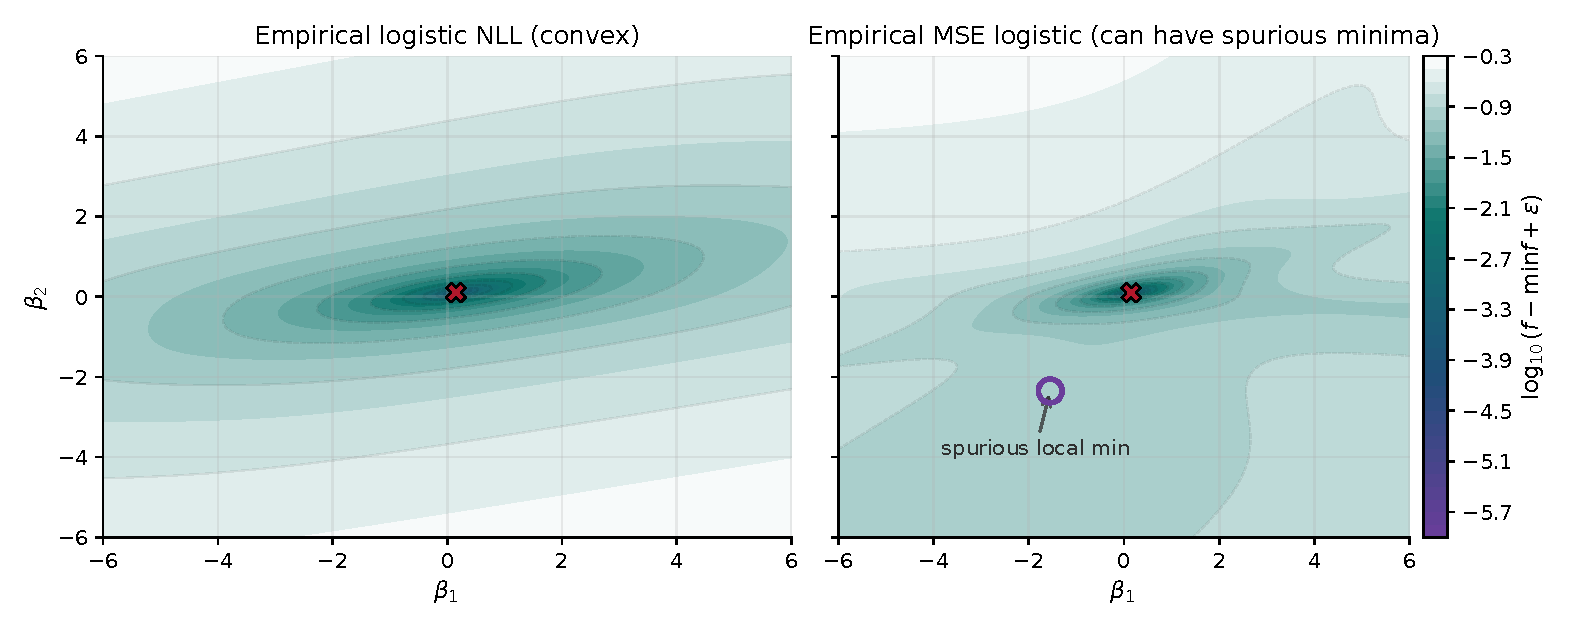
\includegraphics[width=\textwidth]{figures/handouts/convexity_optimization/fig_logistic_empirical_spurious}
  \caption{Empirical logistic landscapes on the dataset in \Cref{ex:logistic-empirical-spurious}.
  The plots show $\log_{10}(f-\min f+\varepsilon)$ for each objective.
  The red X marks the global minimizer in each panel.
  Left: the NLL is convex (one basin).
  Right: the squared-loss objective can have a spurious local minimum (circled), so a local method can get stuck.}
  \label{fig:logistic-empirical-spurious}
\end{figure}

\begin{figure}[t]
  \centering
  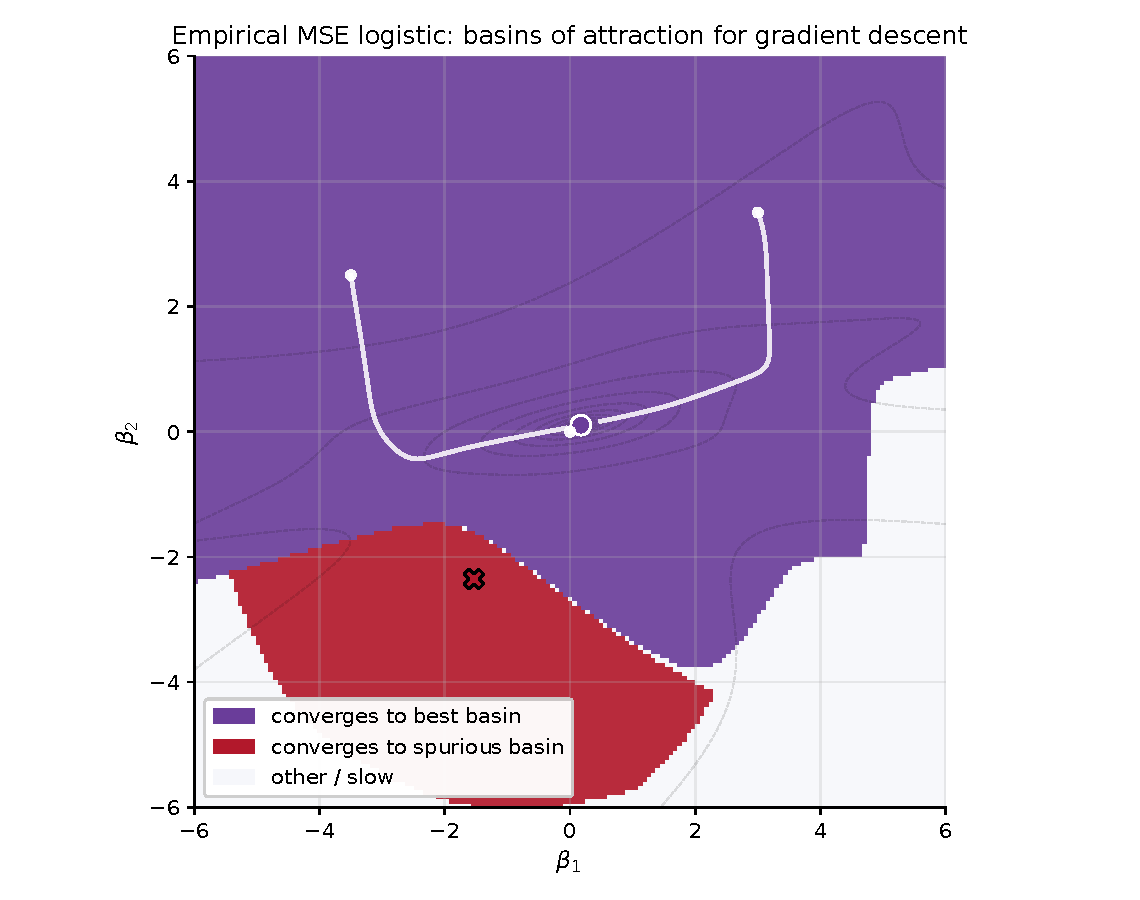
\includegraphics[width=0.92\textwidth]{figures/handouts/convexity_optimization/fig_logistic_empirical_basins}
  \caption{Basins of attraction for gradient descent on the empirical MSE-logistic objective in \Cref{ex:logistic-empirical-spurious}.
  The purple dot and red X mark the two local minimizers.
  Each initialization is colored by which local minimizer fixed-step GD (with $\eta=0.6$) converges to, and the overlaid paths show a few representative trajectories.}
  \label{fig:logistic-empirical-basins}
\end{figure}

Now assume a realizable population model:
\[
Y\mid X=x \sim \mathrm{Bernoulli}(p^\star(x)),
\qquad
p^\star(x) = \sigma(x^\top\beta^\star).
\]
Then the expected squared loss decomposes as
\[
\E\big[(Y-\sigma(X^\top\beta))^2\mid X\big]
= p^\star(X)(1-p^\star(X)) + \big(p^\star(X)-\sigma(X^\top\beta)\big)^2,
\]
so (up to an additive constant) the population objective becomes
\begin{equation}
R(\beta) = \E\big[(\sigma(X^\top\beta)-\sigma(X^\top\beta^\star))^2\big].
\label{eq:logistic-pop-risk}
\end{equation}

\begin{proposition}[One-point monotonicity in the realizable population squared-loss risk]
\label{prop:logistic-pop-one-point}
Assume $\E[\norm{X}_2]<\infty$, and let $R$ be as in \eqref{eq:logistic-pop-risk}. Then for all $\beta$,
\begin{equation}
\ip{\nabla R(\beta)}{\beta-\beta^\star} \ge 0.
\label{eq:one-point}
\end{equation}
In particular, along any ray $\beta(t)=\beta^\star+t(\beta-\beta^\star)$, the function $t\mapsto R(\beta(t))$ is nondecreasing for $t\ge 0$.
\end{proposition}

The next exercise isolates the population monotonicity calculation; structurally it plays the same role as the first-order convexity arguments in the Optimization unit.
\begin{exercise}[One-point monotonicity for realizable MSE-logistic]
\label{ex:logistic-one-point}
Prove \Cref{prop:logistic-pop-one-point}.
Let $\eta=X^\top\beta$ and $\eta^\star=X^\top\beta^\star$.
\begin{enumerate}[leftmargin=*]
  \item Differentiate under the expectation in \eqref{eq:logistic-pop-risk} to show that
  \[
  \nabla R(\beta)
  =2\,\E\Big[(\sigma(\eta)-\sigma(\eta^\star))\,\sigma'(\eta)\,X\Big].
  \]
  \item Show that
  \[
  \ip{\nabla R(\beta)}{\beta-\beta^\star}
  =2\,\E\Big[\sigma'(\eta)\,(\sigma(\eta)-\sigma(\eta^\star))(\eta-\eta^\star)\Big],
  \]
  and conclude it is nonnegative using only that $\sigma$ is increasing and $\sigma'\ge 0$.
  \item Deduce the ray-monotonicity statement by differentiating $g(t)=R(\beta^\star+t(\beta-\beta^\star))$.
\end{enumerate}
\end{exercise}

\SolutionBox[14]{%
\emph{Part (1).}
Differentiate \eqref{eq:logistic-pop-risk} under the expectation:
\[
R(\beta)=\E\big[(\sigma(X^\top\beta)-\sigma(X^\top\beta^\star))^2\big].
\]
Using the chain rule, $\nabla_\beta\sigma(X^\top\beta)=\sigma'(X^\top\beta)\,X$, hence
\[
\nabla R(\beta)
=2\,\E\Big[(\sigma(\eta)-\sigma(\eta^\star))\,\sigma'(\eta)\,X\Big],
\qquad
\eta=X^\top\beta,\ \eta^\star=X^\top\beta^\star.
\]

\emph{Part (2).}
Take the inner product with $(\beta-\beta^\star)$ and use $\ip{X}{\beta-\beta^\star}=\eta-\eta^\star$:
\[
\ip{\nabla R(\beta)}{\beta-\beta^\star}
=2\,\E\Big[\sigma'(\eta)\,(\sigma(\eta)-\sigma(\eta^\star))(\eta-\eta^\star)\Big].
\]
Since $\sigma'(\eta)\ge 0$ and $\sigma$ is increasing, we have
$(\sigma(\eta)-\sigma(\eta^\star))(\eta-\eta^\star)\ge 0$ pointwise.
Therefore the integrand is pointwise nonnegative, and the expectation is nonnegative as claimed.

\emph{Part (3) (ray monotonicity).}
For the ray $\beta(t)=\beta^\star+t(\beta-\beta^\star)$, define $g(t)=R(\beta(t))$.
By the chain rule,
\[
g'(t)=\ip{\nabla R(\beta(t))}{\beta-\beta^\star}\ge 0,
\]
so $t\mapsto R(\beta(t))$ is nondecreasing for $t\ge 0$.
(The argument uses only that the link is increasing with nonnegative derivative, so it holds for any such link function.)%
}

\begin{corollary}[Realizable population MSE-logistic has no spurious local minima]
\label{cor:logistic-pop-no-spurious}
Under the assumptions of \Cref{prop:logistic-pop-one-point}, every local minimizer of the realizable population risk $R$ in \eqref{eq:logistic-pop-risk} is global.
If in addition $\E[XX^\top]\succ 0$, then the unique global minimizer is $\beta^\star$.
\end{corollary}

\begin{exercise}[Stationarity + one-point monotonicity $\Rightarrow$ no spurious local minima]
\label{ex:logistic-one-point-no-spurious}
Prove \Cref{cor:logistic-pop-no-spurious} from \Cref{prop:logistic-pop-one-point}.
\begin{enumerate}[leftmargin=*]
  \item Let $\bar\beta$ be a local minimizer. Since $R$ is differentiable, $\nabla R(\bar\beta)=0$.
  Combine this with \Cref{eq:one-point} to show that
  \[
    0
    = \ip{\nabla R(\bar\beta)}{\bar\beta-\beta^\star}
    = 2\,\E\Big[\sigma'(\bar\eta)\,(\sigma(\bar\eta)-\sigma(\eta^\star))(\bar\eta-\eta^\star)\Big],
  \]
  where $\bar\eta=X^\top\bar\beta$ and $\eta^\star=X^\top\beta^\star$.
  Conclude that $\sigma(X^\top\bar\beta)=\sigma(X^\top\beta^\star)$ almost surely.
  \item Deduce that $R(\bar\beta)=0$, so $\bar\beta$ is a global minimizer.
  \item For uniqueness: show that if $R(\beta)=0$, then $X^\top(\beta-\beta^\star)=0$ almost surely, and deduce $\beta=\beta^\star$ under $\E[XX^\top]\succ 0$.
\end{enumerate}
\end{exercise}

\SolutionBox[14]{%
\emph{Part (1).}
Let $\bar\beta$ be a local minimizer of the differentiable function $R$.
Then $\nabla R(\bar\beta)=0$.
Applying \Cref{prop:logistic-pop-one-point} at $\beta=\bar\beta$ gives
\[
0
= \ip{\nabla R(\bar\beta)}{\bar\beta-\beta^\star}
= 2\,\E\Big[\sigma'(\bar\eta)\,(\sigma(\bar\eta)-\sigma(\eta^\star))(\bar\eta-\eta^\star)\Big],
\qquad \bar\eta=X^\top\bar\beta,\ \eta^\star=X^\top\beta^\star.
\]
The integrand is pointwise nonnegative because $\sigma'(\bar\eta)\ge 0$ and $\sigma$ is increasing, so the expectation can vanish only if the integrand is zero almost surely.
Since $\sigma'(z)>0$ for every finite $z$, this implies
\[
(\sigma(\bar\eta)-\sigma(\eta^\star))(\bar\eta-\eta^\star)=0
\qquad\text{almost surely.}
\]
Because $\sigma$ is strictly increasing, the product above is zero if and only if $\bar\eta=\eta^\star$, equivalently $\sigma(X^\top\bar\beta)=\sigma(X^\top\beta^\star)$ almost surely.

\emph{Part (2).}
If $\sigma(X^\top\bar\beta)=\sigma(X^\top\beta^\star)$ almost surely, then the integrand in \eqref{eq:logistic-pop-risk} vanishes almost surely, so
\[
R(\bar\beta)=\E\big[(\sigma(X^\top\bar\beta)-\sigma(X^\top\beta^\star))^2\big]=0.
\]
Since $R(\beta^\star)=0$ as well, $\bar\beta$ is a global minimizer.

\emph{Part (3) (uniqueness).}
If $R(\beta)=0$, then
\[
\E\big[(\sigma(X^\top\beta)-\sigma(X^\top\beta^\star))^2\big]=0,
\]
so $\sigma(X^\top\beta)=\sigma(X^\top\beta^\star)$ almost surely.
Since $\sigma$ is strictly increasing, this implies $X^\top(\beta-\beta^\star)=0$ almost surely.
Taking expectations yields
$(\beta-\beta^\star)^\top\E[XX^\top](\beta-\beta^\star)=0$.
If $\E[XX^\top]\succ 0$, then the quadratic form is strictly positive unless $\beta=\beta^\star$, so $\beta^\star$ is the unique global minimizer.%
}

The population MSE-logistic risk is nonconvex, but it still has the simple geometry that moving away from $\beta^\star$ does not help along any ray from $\beta^\star$.
This is qualitatively different from objectives like ecological logistic regression (\Cref{sec:ecological-logistic}), where aggregation introduces intrinsic nonconvexity and the landscape can have many distinct basins even under a clean population model.

Even with this benign global geometry, gradient descent can be slow because of saturation and flat plateaus.
The one-point monotonicity in \Cref{prop:logistic-pop-one-point} is a global geometry guarantee, but it is not a rate guarantee.
Far from $\beta^\star$, the squared-loss logistic objective can become very flat because the logistic link saturates:
$\sigma(z)\to 0$ or $1$ and $\sigma'(z)\to 0$ as $|z|\to\infty$.
The squared-loss gradient carries a factor of $\sigma'(X^\top\beta)$, so when the model is very confident (large $|X^\top\beta|$), the gradient can be tiny even if the objective value is not close to its minimum.
This mirrors the ``confidence weights'' story for convex NLL objectives:
in logistic NLL, curvature is largest near the decision boundary, while very confident points contribute little.
For squared loss, that same saturation suppresses the \emph{descent signal} itself, producing plateaus where $\norm{\nabla R(\beta)}_2$ is small even though $R(\beta)-R(\beta^\star)$ is not.

\begin{proposition}[Realizable squared-loss logistic: arbitrarily flat far from $\beta^\star$]
\label{prop:logistic-pop-flat}
Assume $\E[\norm{X}_2]<\infty$ and let $R$ be the realizable population risk \eqref{eq:logistic-pop-risk}.
Define $g(t)=R(t\beta^\star)$ for $t\ge 1$.
Then:
\begin{enumerate}[leftmargin=*]
  \item $g$ is nondecreasing on $[1,\infty)$ and converges to a finite limit $g(\infty)$.
  \item $\lim_{t\to\infty} g'(t)=0$ and $\lim_{t\to\infty}\norm{\nabla R(t\beta^\star)}_2=0$.
  \item If $\Pr(X^\top\beta^\star\neq 0)>0$, then $g(\infty)>0$.
\end{enumerate}
In particular, there are directions along which the landscape becomes arbitrarily flat even though the excess risk stays bounded away from $0$.
\end{proposition}

\emph{Proof idea.} See Exercise~\ref{ex:logistic-plateau}.

\begin{exercise}[Prove the plateau]
\label{ex:logistic-plateau}
In the realizable population model, let $g(t)=R(t\beta^\star)$ for $t\ge 1$.
\begin{enumerate}[leftmargin=*]
  \item Show that
  \[
    g'(t)=2\,\E\big[(\sigma(t\eta^\star)-\sigma(\eta^\star))\,\sigma'(t\eta^\star)\,\eta^\star\big],
    \qquad \eta^\star=X^\top\beta^\star,
  \]
  and conclude that $g$ is nondecreasing (hence $g(t)\to g(\infty)$ since $0\le g(t)\le 1$).
  \item Show that $g'(t)\to 0$ and $\nabla R(t\beta^\star)\to 0$ as $t\to\infty$.
  Interpret this as: \emph{without} a PL/strong-convexity-type condition, small gradient does not imply near-optimality.
  \item Assume $\Pr(\eta^\star\neq 0)>0$.
  Show that $g(\infty)>0$.
\end{enumerate}
\end{exercise}

\SolutionBox[12]{%
Write $\eta^\star=X^\top\beta^\star$ so that $g(t)=\E[(\sigma(t\eta^\star)-\sigma(\eta^\star))^2]$.

\emph{Part (1).}
Differentiate under the expectation:
by the chain rule,
\[
\frac{d}{dt}\sigma(t\eta^\star)=\sigma'(t\eta^\star)\,\eta^\star,
\]
so
\[
g'(t)
=\E\Big[2(\sigma(t\eta^\star)-\sigma(\eta^\star))\cdot \sigma'(t\eta^\star)\,\eta^\star\Big]
=2\,\E\big[(\sigma(t\eta^\star)-\sigma(\eta^\star))\,\sigma'(t\eta^\star)\,\eta^\star\big].
\]
For $t\ge 1$, $\sigma(t\eta^\star)-\sigma(\eta^\star)$ has the same sign as $(t-1)\eta^\star$ since $\sigma$ is increasing.
Because $\sigma'\ge 0$, the integrand is pointwise nonnegative, hence $g'(t)\ge 0$ and $g$ is nondecreasing.
Since $g(t)\in[0,1]$, it follows that $g(t)\to g(\infty)$ for some finite limit $g(\infty)$.

\emph{Part (2).}
For each fixed $\eta^\star\neq 0$, we have $t\eta^\star\to \pm\infty$ and therefore $\sigma'(t\eta^\star)\to 0$ as $t\to\infty$.
Also,
\[
\big|(\sigma(t\eta^\star)-\sigma(\eta^\star))\,\sigma'(t\eta^\star)\,\eta^\star\big|
\le \sigma'(0)\,|\eta^\star|
\le \sigma'(0)\,\norm{\beta^\star}_2\,\norm{X}_2,
\]
which is integrable since $\E[\norm{X}_2]<\infty$.
We will use the following standard fact: if random variables $Z_t$ satisfy $|Z_t|\le W$ with $\E[W]<\infty$ and $Z_t\to 0$ almost surely, then $\E[Z_t]\to 0$.
Applying this fact here gives $g'(t)\to 0$ as $t\to\infty$.

\smallskip
Similarly, differentiating \eqref{eq:logistic-pop-risk} gives
\[
\nabla R(t\beta^\star)
=2\,\E\big[(\sigma(t\eta^\star)-\sigma(\eta^\star))\,\sigma'(t\eta^\star)\,X\big].
\]
The integrand norm is bounded by $2\sigma'(0)\norm{X}_2$, and for each fixed $X$ the factor $\sigma'(t\eta^\star)$ tends to $0$ (or the bracketed term vanishes when $\eta^\star=0$), so the same reasoning lets us pass the limit through the expectation and conclude $\nabla R(t\beta^\star)\to 0$.

\emph{Part (3).}
As $t\to\infty$ we have $\sigma(t\eta^\star)\to 1$ when $\eta^\star>0$, $\sigma(t\eta^\star)\to 0$ when $\eta^\star<0$, and $\sigma(t\eta^\star)=\sigma(\eta^\star)=1/2$ when $\eta^\star=0$.
Since $0\le (\sigma(t\eta^\star)-\sigma(\eta^\star))^2\le 1$, we can apply the same fact (with $W=1$) to pass the limit through the expectation and obtain
\[
g(\infty)=\E\Big[(1-\sigma(\eta^\star))^2\mathbf{1}\{\eta^\star>0\} + \sigma(\eta^\star)^2\mathbf{1}\{\eta^\star<0\}\Big].
\]
If $\Pr(\eta^\star\neq 0)>0$, then the integrand is strictly positive on $\{\eta^\star\neq 0\}$, so $g(\infty)>0$.

Along this ray, the risk can remain bounded away from $0$ while the gradient (and directional derivative) goes to $0$.
Without a condition like PL/strong convexity, a small gradient does not by itself certify near-optimality.
}

Conditions like strong convexity or the PL inequality (\Cref{def:pl-inequality}) prevent this phenomenon: they rule out large flat regions away from the optimum by relating gradient size to suboptimality.
\Cref{prop:logistic-pop-flat} shows the realizable squared-loss logistic risk does not have such a global guarantee in general.

In the realizable population model, the one-point monotonicity in \Cref{prop:logistic-pop-one-point} is a \emph{global} geometric statement.
To get an actual rate for gradient descent, we also need a \emph{local curvature} condition near $\beta^\star$.
One simple sufficient condition is bounded features, which implies local strong convexity (hence a linear rate) around the optimum.

\begin{proposition}[Local linear convergence of gradient descent near $\beta^\star$]
\label{prop:logistic-pop-local-rate}
Assume $\E[XX^\top]\succeq \lambda I_d$ and $\norm{X}_2\le R$ almost surely for some $\lambda,R>0$.
Then at $\beta^\star$,
\[
\Hess R(\beta^\star)\succeq m_0 I_d,
\qquad
m_0 = 2\,\sigma'(R\norm{\beta^\star}_2)^2\,\lambda,
\]
and there exist $r>0$ and constants $0<m\le L<\infty$ such that the population risk $R$ in \eqref{eq:logistic-pop-risk} is $m$-strongly convex and $L$-smooth on the ball $\{\beta:\ \norm{\beta-\beta^\star}_2\le r\}$.
Consequently, gradient descent with step size $1/L$ initialized in this ball satisfies
\[
R(\beta^{(k)})-R(\beta^\star)
\le \left(1-\frac{m}{L}\right)^k\bigl(R(\beta^{(0)})-R(\beta^\star)\bigr)
\qquad\text{(see \citealp[\S9.3]{boyd_vandenberghe_2004_convex}).}
\]
\end{proposition}

\begin{proof}
Differentiate \eqref{eq:logistic-pop-risk} twice.
At $\beta=\beta^\star$, the cross term vanishes and the Hessian simplifies to
\[
\Hess R(\beta^\star)=2\,\E\big[\sigma'(X^\top\beta^\star)^2\,XX^\top\big].
\]
Since $\norm{X^\top\beta^\star}\le \norm{X}_2\norm{\beta^\star}_2\le R\norm{\beta^\star}_2$ almost surely, we have
$\sigma'(X^\top\beta^\star)\ge \sigma'(R\norm{\beta^\star}_2)>0$ almost surely (since $\sigma'$ is even and decreases with $|z|$), hence
\[
\Hess R(\beta^\star)\succeq 2\,\sigma'(R\norm{\beta^\star}_2)^2\,\E[XX^\top]\succeq 2\,\sigma'(R\norm{\beta^\star}_2)^2\,\lambda I_d.
\]
This is the claimed bound with $m_0=2\,\sigma'(R\norm{\beta^\star}_2)^2\,\lambda$.
Because $R$ is twice continuously differentiable and $\norm{X}_2\le R$ almost surely, $\Hess R(\beta)$ varies continuously in $\beta$ and is bounded on compact sets.
Therefore, on a sufficiently small ball around $\beta^\star$, the Hessian is bounded below by (say) $\tfrac12 m_0 I_d$ and above by $L I_d$ for some finite $L$, which gives local strong convexity and smoothness.
The linear convergence rate for gradient descent on an $m$-strongly convex and $L$-smooth function is standard (cited above).
\end{proof}

Under misspecification, hard multimodality can return.
If $p^\star(x)$ is not representable as $\sigma(x^\top\beta)$ (e.g.\ marginalizing over latent classes can yield mixtures of logits), then \eqref{eq:one-point} need not hold, and the population squared-loss risk can become bimodal with spurious local minima.
Benign global geometry often hinges on model and data assumptions.
This is one reason MLE (convex NLL) is often more stable than squared-loss fitting in logistic-type binary regression models.

\begin{example}[Misspecification can create a spurious local minimum for squared-loss logistic regression]
\label{ex:logistic-misspecified-spurious}
Consider a 1D feature $X$ that takes values $\{-2,-1,1,2\}$ with equal probability, and parameterize $\beta=(\beta_0,\beta_1)$ so that $q_\beta(x)=\sigma(\beta_0+\beta_1 x)$.
Let the true conditional probabilities be
\[
p^\star(-2)=0.49,\quad p^\star(-1)=0.87,\quad p^\star(1)=0.92,\quad p^\star(2)=0.36.
\]
This $p^\star$ is not representable as $q_\beta$, since it is not monotone in $x$.

For the population squared-loss risk $R_{\mathrm{MSE}}(\beta)=\E[(q_\beta(X)-p^\star(X))^2]$, a direct evaluation shows two distinct basins:
numerically, evaluating $R_{\mathrm{MSE}}$ on a grid reveals a global minimizer and a spurious local minimizer.
See \Cref{fig:logistic-landscape-2d}.
\end{example}

\begin{figure}[t]
  \centering
  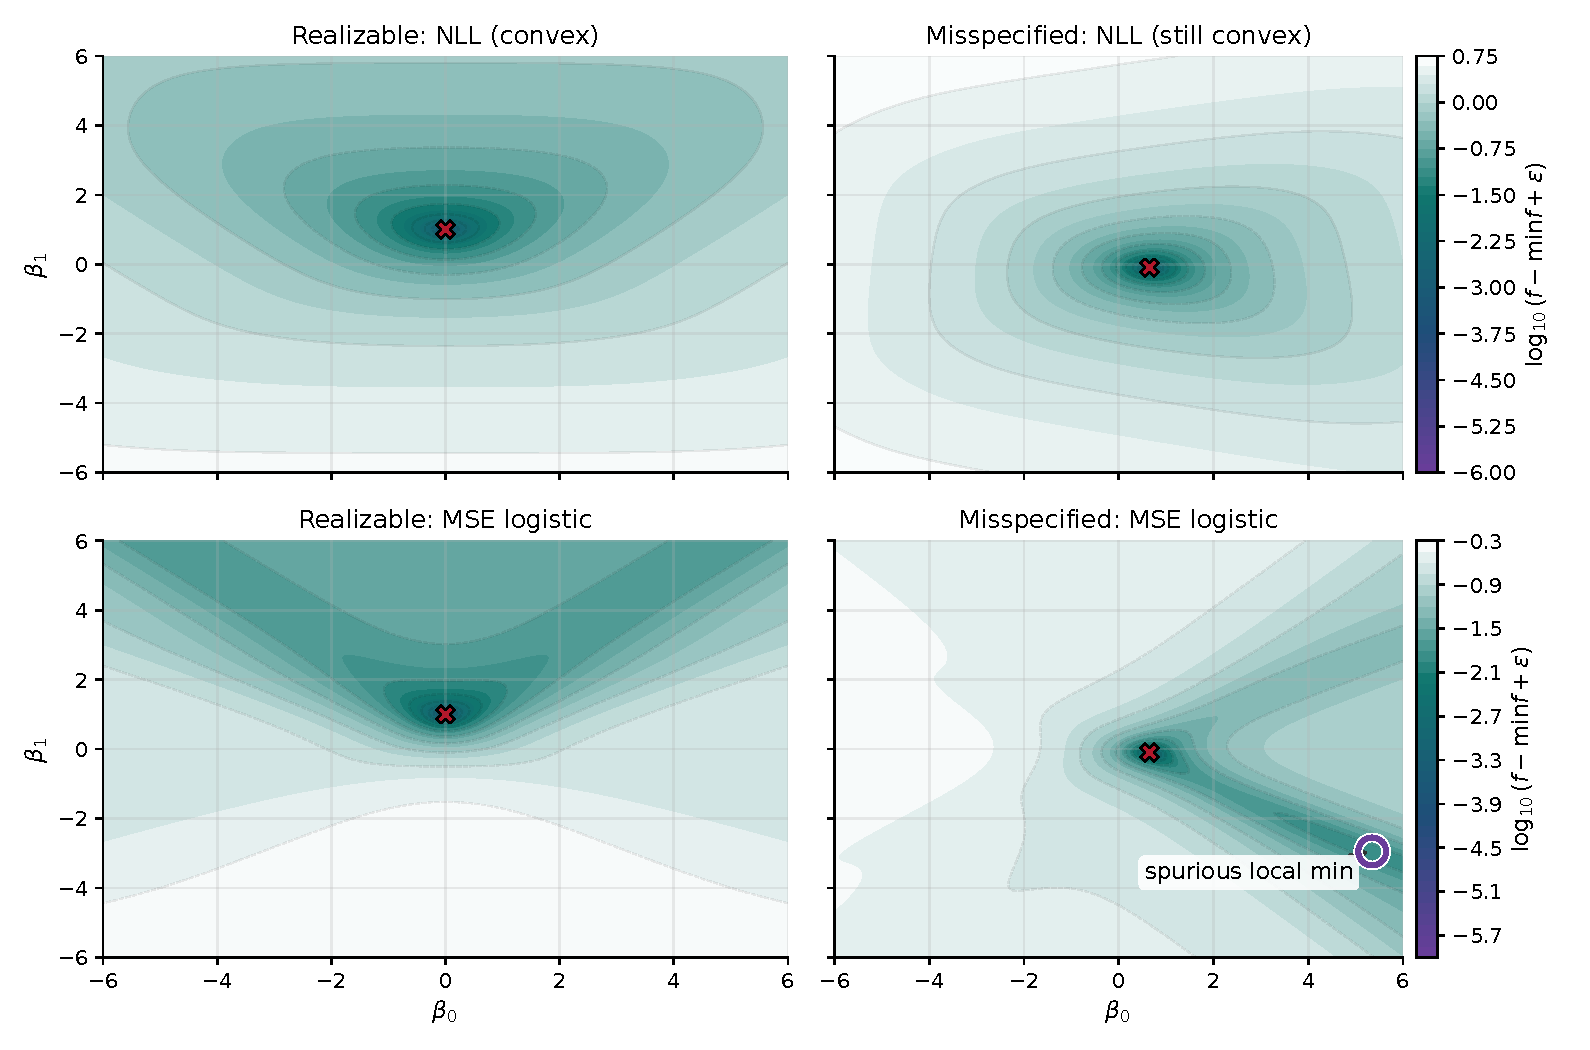
\includegraphics[width=\textwidth]{figures/handouts/convexity_optimization/fig_logistic_landscape_2d}
  \caption{A consistent contourf view of logistic landscapes in a 2D parameterization $\beta=(\beta_0,\beta_1)$.
  The plots show $\log_{10}(f-\min f+\varepsilon)$ for each objective, which makes basins comparable across panels.
  The red X marker indicates the global minimizer in each panel; in the bottom-right plot, the circled point is a spurious local minimum.
  In this example, the NLL landscape is unimodal in both realizable and misspecified settings, while the squared-loss landscape can develop extra basins under misspecification.}
  \label{fig:logistic-landscape-2d}
\end{figure}

% ------------------------------------------------------------
Example~I separates three distinct regimes.
Empirical MSE-logistic can create spurious basins; the realizable population risk has no spurious local minima but can still be slow because of broad plateaus; and misspecification can bring back genuinely wrong stable basins.
The response depends on the regime: use a stable objective when possible, use damping or line search when curvature is unreliable, and use restarts or stronger initializations when multiple basins are present.

% ------------------------------------------------------------
\section[Example II (phase retrieval)]{Example II: multimodality from symmetry, but only global optima in phase retrieval}
\label{sec:phase-retrieval}

In coherent diffraction imaging, optics, and astronomy, sensors measure intensities and lose phase.
A canonical real model is \emph{phase retrieval}:
\[
y_i = (a_i^\top x^\star)^2,\qquad i=1,\dots,m,
\]
where $x^\star\in\R^d$ is the unknown signal and $a_i$ are known sensing vectors.
A standard nonconvex least-squares objective is
\begin{equation}
F(x)=\frac{1}{4m}\sum_{i=1}^m\big((a_i^\top x)^2 - y_i\big)^2.
\label{eq:phase-empirical}
\end{equation}
This objective is nonconvex for structural reasons (it involves squares of linear forms),
and it is \emph{inherently} multimodal because $x^\star$ and $-x^\star$ generate the same data.

Like squared-loss logistic regression, phase retrieval is a smooth, nonconvex least-squares objective.
But here the nonconvexity is driven primarily by a \emph{symmetry}: $x^\star$ and $-x^\star$ generate the same data.
In population (for Gaussian designs), this symmetry produces multiple global optima but \emph{no} suboptimal local minima; the remaining stationary points are saddles.
This is ``benign'' nonconvexity (a strict-saddle picture), and it contrasts with ecological logistic regression (\Cref{sec:ecological-logistic}), where aggregation creates intrinsic nonconvexity and can lead to many distinct basins.
This ``benign geometry'' picture (multiple equivalent global minimizers; strict saddles elsewhere) appears broadly in modern tractable nonconvex problems; see \citet[\S2]{sun_qu_wright_2015_nonconvex_not_scary} and \citet[\S1]{zhang_qu_wright_2020_symmetry_geometry}.

\begin{figure}[t]
  \centering
  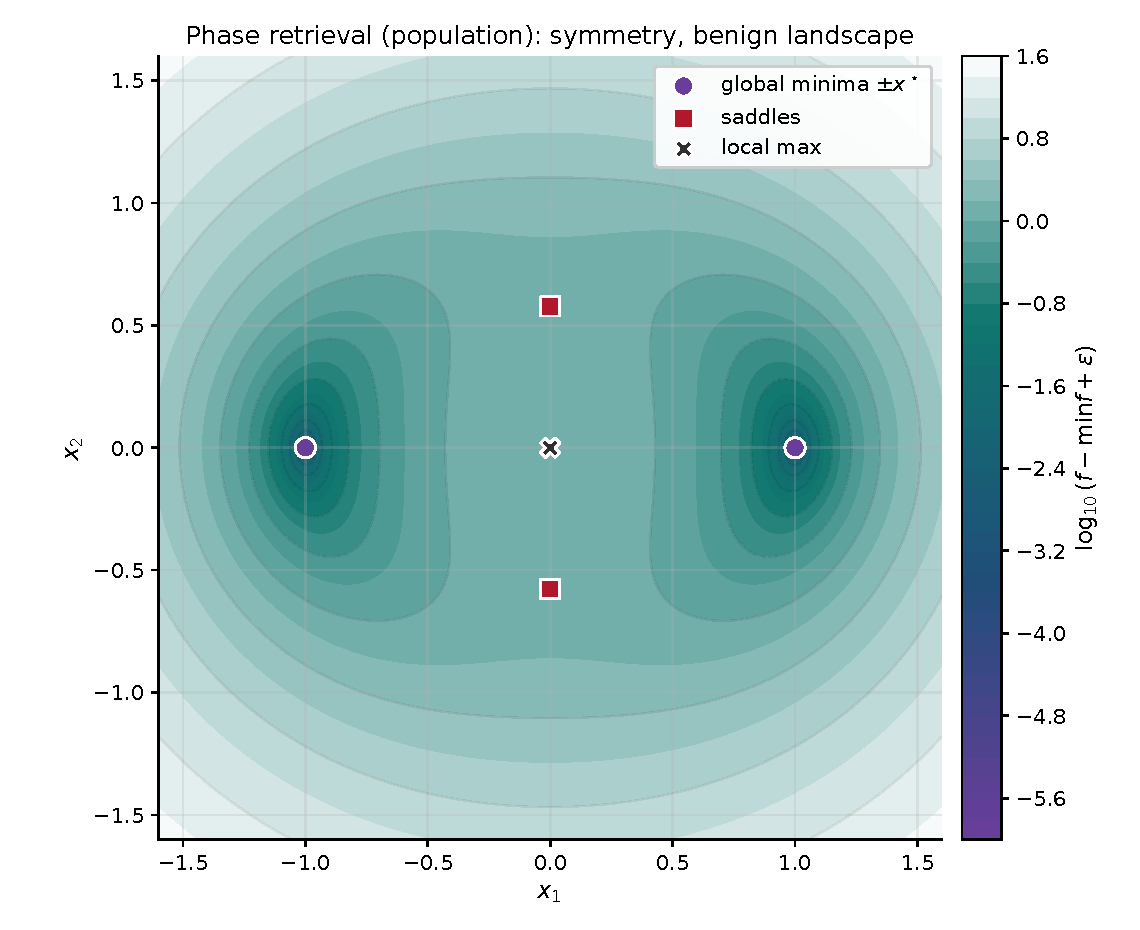
\includegraphics[width=0.86\textwidth]{figures/handouts/convexity_optimization/fig_phase_retrieval_landscape}
  \caption{Population phase retrieval in $d=2$: the landscape is nonconvex and symmetric ($x\sim -x$), but the only local minima are the two global minima $\pm x^\star$; other critical points are saddles or a local maximum at the origin.}
  \label{fig:phase-retrieval-landscape}
\end{figure}

For a clean population model, assume $a\sim N(0,I_d)$ and consider the \emph{population} objective
\begin{equation}
  f(x)=\frac12\,\E\Big[\big((a^\top x)^2 - (a^\top x^\star)^2\big)^2\Big].
  \label{eq:phase-pop}
\end{equation}

\begin{proposition}[Population phase retrieval: nonconvex but no spurious local minima]
\label{prop:phase-retrieval-benign}
For $f$ in \eqref{eq:phase-pop},
\begin{equation}
  f(x)
  =\frac{3}{2}\norm{x}^4 - \norm{x}^2\norm{x^\star}^2 - 2\ip{x}{x^\star}^2 + \frac{3}{2}\norm{x^\star}^4,
  \label{eq:phase-pop-closed-form}
\end{equation}
and the stationary points are:
\begin{enumerate}[leftmargin=*]
  \item global minima $x=\pm x^\star$ (value $0$),
  \item a local maximum at $x=0$,
  \item a saddle set $\{x:\ x\perp x^\star,\ \norm{x}=\norm{x^\star}/\sqrt{3}\}$.
\end{enumerate}
In particular, every local minimum is global.
\end{proposition}

\begin{exercise}[Phase retrieval: derive and classify the population stationary points]
\label{ex:phase-pop-derivation}
Prove \Cref{prop:phase-retrieval-benign}.
\begin{enumerate}[leftmargin=*]
  \item Expand \eqref{eq:phase-pop} and use the Gaussian fourth-moment identities
  \[
  \E[(a^\top u)^4]=3\norm{u}^4,
  \qquad
  \E[(a^\top u)^2(a^\top v)^2]=\norm{u}^2\norm{v}^2 + 2\ip{u}{v}^2,
  \]
  to obtain \eqref{eq:phase-pop-closed-form}.
  \item Differentiate \eqref{eq:phase-pop-closed-form} to get an explicit formula for $\nabla f(x)$.
  \item Solve $\nabla f(x)=0$ by decomposing $x=\alpha x^\star + u$ with $u\perp x^\star$.
  \item Classify the stationary points as global minima, a local maximum, and a saddle set.
\end{enumerate}
\end{exercise}

\SolutionBox[22]{%
\emph{Part (1) (closed form).}
Expanding the square in \eqref{eq:phase-pop} gives
\[
f(x)
=\frac12\,\E\big[(a^\top x)^4\big]
\;-\;\E\big[(a^\top x)^2(a^\top x^\star)^2\big]
\;+\;\frac12\,\E\big[(a^\top x^\star)^4\big].
\]
Apply the stated Gaussian fourth-moment identities with $u=x$ and $v=x^\star$ to get
\[
\E[(a^\top x)^4]=3\norm{x}^4,\qquad
\E[(a^\top x^\star)^4]=3\norm{x^\star}^4,
\]
and
\[
\E[(a^\top x)^2(a^\top x^\star)^2]=\norm{x}^2\norm{x^\star}^2 + 2\ip{x}{x^\star}^2.
\]
Substituting yields \eqref{eq:phase-pop-closed-form}.

\emph{Part (2) (gradient).}
Differentiate \eqref{eq:phase-pop-closed-form}:
\[
\nabla f(x)
= 6\norm{x}^2 x - 2\norm{x^\star}^2 x - 4\ip{x}{x^\star}x^\star
= (6\norm{x}^2-2\norm{x^\star}^2)x - 4\ip{x}{x^\star}x^\star.
\]

\emph{Part (3) (stationary points).}
Let $r=\norm{x^\star}_2$ and decompose $x=\alpha x^\star + u$ with $u\perp x^\star$.
Then $\ip{x}{x^\star}=\alpha r^2$ and $\norm{x}^2=\alpha^2r^2+\norm{u}^2$.
Setting $\nabla f(x)=0$ and matching the $u$ and $x^\star$ components gives
\[
(6\norm{x}^2-2r^2)\,u=0,
\qquad
\alpha\,(6\norm{x}^2-6r^2)=0.
\]
If $u=0$, then either $\alpha=0$ (so $x=0$) or $\norm{x}^2=r^2$ (so $\alpha=\pm 1$ and $x=\pm x^\star$).
If $u\neq 0$, then the first equation forces $\norm{x}^2=r^2/3$, and the second forces $\alpha=0$, hence
$x\perp x^\star$ and $\norm{x}=r/\sqrt{3}$.
This gives exactly the stationary-point list in \Cref{prop:phase-retrieval-benign}.

\emph{Part (4) (classification).}
Since $f$ in \eqref{eq:phase-pop} is an expectation of a square, $f(x)\ge 0$ for all $x$.
Also $f(\pm x^\star)=0$, so $\pm x^\star$ are global minima.

For $x=0$, the expansion \eqref{eq:phase-pop-closed-form} shows
\[
f(0)-f(x)= r^2\norm{x}^2 + 2\ip{x}{x^\star}^2 - \frac{3}{2}\norm{x}^4,
\]
which is strictly positive for all sufficiently small $x\neq 0$ (the quadratic term dominates), so $x=0$ is a local maximum.

Finally, if $x\perp x^\star$ and $\norm{x}=r/\sqrt{3}$, then the univariate restriction $t\mapsto f(x+t x^\star)$ has negative second derivative at $t=0$, so there is a direction of negative curvature.
Hence these points are saddles, and every local minimum is global.%
}

This is symmetry-driven nonconvexity with a strict-saddle geometry:
every non-optimal stationary point has a direction of negative curvature.

Phase retrieval is typically approached via the two-stage template in \Cref{alg:two-stage-template}:
use a cheap global initializer, then run a local method.
In the Gaussian model, there is a clean way to build a provably good direction estimate from a simple moment identity.
Assume the noiseless Gaussian design model $a_i \stackrel{\mathrm{iid}}{\sim} N(0,I_d)$ with measurements $y_i=(a_i^\top x^\star)^2$.
Define the \emph{spectral matrix}
\[
  Y = \frac{1}{m}\sum_{i=1}^m y_i a_i a_i^\top.
\]
Also define the radius estimate
\[
  \hat r^2 = \frac{1}{m}\sum_{i=1}^m y_i,
\]
which satisfies $\E[\hat r^2]=\norm{x^\star}_2^2$.
If $\hat u$ is a unit-norm top eigenvector of $Y$, then the standard spectral initializer is $x^{(0)}=\hat r\,\hat u$.

The next proposition explains why this initialization is reasonable.
It shows that (i) the population matrix $\E[Y]$ has a unique leading eigenvector in the $x^\star$ direction, and (ii) if the empirical $Y$ is close to $\E[Y]$ in operator norm then its leading eigenvector must be close to $\pm x^\star/\norm{x^\star}_2$.
(Here $\norm{M}_{\mathrm{op}}$ denotes the operator norm, i.e.\ the largest absolute eigenvalue for a symmetric matrix $M$.)

\begin{proposition}[Gaussian phase retrieval: why the spectral initializer points at $x^\star$]
\label{prop:phase-spectral-init}
Assume $x^\star\neq 0$, let $a\sim N(0,I_d)$, and set $y=(a^\top x^\star)^2$.
Write $r=\norm{x^\star}_2$ and $u^\star=x^\star/r$.
Define the population matrix
\[
  Y_{\mathrm{pop}} = \E\big[y\,a a^\top\big]
  = \E\big[(a^\top x^\star)^2 a a^\top\big].
\]
Then
\[
  Y_{\mathrm{pop}}=r^2 I_d + 2x^\star(x^\star)^\top,
\]
so the unique leading eigenvector of $Y_{\mathrm{pop}}$ is $u^\star$.
Moreover, if $Y$ is any symmetric matrix satisfying
\[
\norm{Y-Y_{\mathrm{pop}}}_{\mathrm{op}} \le \varepsilon\, r^2
\qquad\text{for some }\varepsilon\in(0,1),
\]
then for every unit-norm leading eigenvector $\hat u$ of $Y$ there exists a sign $s\in\{\pm 1\}$ such that
$\norm{\hat u-su^\star}_2\le \sqrt{2\varepsilon}$.
\end{proposition}

\begin{exercise}[Phase retrieval: why spectral initialization points at $x^\star$]
\label{ex:phase-spectral-spike}
Prove \Cref{prop:phase-spectral-init}.
Conclude that if the empirical matrix $Y$ is close to $Y_{\mathrm{pop}}$ in operator norm, then its top eigenvector is close to $\pm u^\star$ and the spectral initializer $x^{(0)}=\hat r\,\hat u$ is close to $\pm x^\star$.
\emph{Hint:} to compute $Y_{\mathrm{pop}}$, you can either compute entries using the Gaussian fourth-moment identity
$\E[a_i a_j a_k a_\ell]=\delta_{ij}\delta_{k\ell}+\delta_{ik}\delta_{j\ell}+\delta_{i\ell}\delta_{jk}$,
or compute the entries directly by expanding.
For the perturbation bound, compare quadratic forms $v^\top Y v$ and use $|v^\top (Y-Y_{\mathrm{pop}}) v|\le \norm{Y-Y_{\mathrm{pop}}}_{\mathrm{op}}$ for unit $v$.
Finally, explain in a sentence why one expects $\norm{Y-Y_{\mathrm{pop}}}_{\mathrm{op}}$ to be small when $m$ is large in the Gaussian model.
\end{exercise}

\SolutionBox[20]{%
Write $u=x^\star$ and expand $y=(a^\top u)^2=\sum_{k,\ell} u_k u_\ell a_k a_\ell$.
For each entry $(i,j)$,
\[
\E\!\big[y\,a_i a_j\big]
=\sum_{k,\ell} u_k u_\ell\,\E[a_i a_j a_k a_\ell]
=\sum_{k,\ell} u_k u_\ell\bigl(\delta_{ij}\delta_{k\ell}+\delta_{ik}\delta_{j\ell}+\delta_{i\ell}\delta_{jk}\bigr).
\]
The first term gives $\delta_{ij}\sum_k u_k^2=\delta_{ij}\norm{u}_2^2$.
The second and third terms each give $u_i u_j$.
Thus $\E[y\,a_i a_j]=\norm{u}_2^2\,\delta_{ij}+2u_i u_j$, i.e.
$Y_{\mathrm{pop}}=\norm{u}_2^2 I_d + 2uu^\top$.

For eigenvalues, note that $Y_{\mathrm{pop}}u=(\norm{u}_2^2+2\norm{u}_2^2)u=3\norm{u}_2^2 u$.
If $w\perp u$, then $uu^\top w=0$ so $Y_{\mathrm{pop}}w=\norm{u}_2^2 w$.
Hence the unique top eigenspace is $\mathrm{span}\{u\}$.

Let $r=\norm{u}_2$ and $u^\star=u/r$.
Let $\hat u$ be a unit top eigenvector of $Y$.
Write $E=Y-Y_{\mathrm{pop}}$ and assume $\norm{E}_{\mathrm{op}}\le \varepsilon r^2$.
Then
\[
\hat u^\top Y_{\mathrm{pop}} \hat u
= \hat u^\top Y \hat u - \hat u^\top E \hat u
\ge \lambda_{\max}(Y) - \norm{E}_{\mathrm{op}}
\ge (u^\star)^\top Y u^\star - \norm{E}_{\mathrm{op}}
\ge 3r^2 - 2\varepsilon r^2.
\]
On the other hand,
$
\hat u^\top Y_{\mathrm{pop}} \hat u
= r^2 + 2r^2\,|\ip{\hat u}{u^\star}|^2.
$
Combining gives $|\ip{\hat u}{u^\star}|^2\ge 1-\varepsilon$.
Choosing the sign that maximizes the inner product,
\[
\min\{\norm{\hat u-u^\star}_2,\norm{\hat u+u^\star}_2\}^2
=2\bigl(1-|\ip{\hat u}{u^\star}|\bigr)
\le 2\bigl(1-|\ip{\hat u}{u^\star}|^2\bigr)
\le 2\varepsilon.
\]

The matrix $Y$ is an empirical average of i.i.d.\ symmetric matrices with mean $Y_{\mathrm{pop}}$.
To make this quantitative in high dimensions, one uses concentration inequalities for random matrices to bound $\norm{Y-Y_{\mathrm{pop}}}_{\mathrm{op}}$ with high probability; see \citet[\S2.2]{zhang_qu_wright_2020_symmetry_geometry} for discussion and references.
These probability tools are largely orthogonal to our focus here.%
}

Once you have an initialization that is close to $\pm x^\star$, the local stage behaves like the convex story again.
In the Gaussian population objective, $\pm x^\star$ are not only global minima: they are \emph{locally strongly convex} minima, so the standard local strong-convexity analysis from the Optimization unit gives a linear rate while the iterates remain in that neighborhood.

\begin{exercise}[Phase retrieval: local convexity near $\pm x^\star$ in the population objective]
\label{ex:phase-pop-local-strong-convex}
For the population objective $f$ in \eqref{eq:phase-pop-closed-form}, compute the Hessian $\Hess f(x)$ and show that
\[
\Hess f(x^\star)=4\norm{x^\star}_2^2 I_d + 8x^\star(x^\star)^\top.
\]
Deduce the eigenvalues of $\Hess f(x^\star)$ and interpret this as a local condition-number statement near $x^\star$.
\end{exercise}

\SolutionBox[12]{%
Differentiate the gradient formula in the solution to \Cref{ex:phase-pop-derivation}:
for $x\in\R^d$,
\[
\Hess f(x)=12xx^\top + (6\norm{x}_2^2-2\norm{x^\star}_2^2)I_d - 4x^\star(x^\star)^\top.
\]
At $x=x^\star$ this becomes
\[
\Hess f(x^\star)=(12-4)x^\star(x^\star)^\top + 4\norm{x^\star}_2^2 I_d
=8x^\star(x^\star)^\top + 4\norm{x^\star}_2^2 I_d.
\]
Along $u^\star=x^\star/\norm{x^\star}_2$ the eigenvalue is $12\norm{x^\star}_2^2$, and along any direction orthogonal to $x^\star$ the eigenvalue is $4\norm{x^\star}_2^2$.
So near $x^\star$ the population objective is well conditioned (local condition number $3$), which is exactly the regime where local methods behave like in the convex case.%
}

These pieces give the standard Gaussian-model story:
spectral initialization supplies a direction close to $\pm x^\star$, and the local geometry near $\pm x^\star$ is strongly convex, so local methods converge quickly once initialized there.
Rigorous finite-sample analyses follow this template; see \citet[\S2.2]{zhang_qu_wright_2020_symmetry_geometry} and references therein.

Phase retrieval shows a different kind of nonconvexity.
The sign symmetry creates multiple optima, but they are equivalent, and the remaining stationary points are saddles rather than bad local minima.
The right response is therefore not exhaustive global search; it is a coarse initializer, such as a spectral method, followed by local refinement inside the basin of $\pm x^\star$.



% ------------------------------------------------------------
\section[Example III (ecological logistic)]{Example III: hard nonconvexity from aggregation in ecological logistic regression}
\label{sec:ecological-logistic}

In some applications we observe covariates at the unit level but only aggregated outcomes.
For example, we might see covariates $x_{g,1},\dots,x_{g,n_g}$ for individuals in a group (a precinct, a cohort, a batch),
but instead of observing the binary outcomes $Y_{g,i}\in\{0,1\}$ we only observe the group total
\[
Z_g = \sum_{i=1}^{n_g} Y_{g,i}.
\]
Many different binary vectors $(Y_{g,1},\dots,Y_{g,n_g})$ can produce the same total $Z_g$, so the likelihood for $\beta$ must marginalize over a large discrete set of latent ``assignments.''

Assume a logistic model at the unit level:
\[
\Pr(Y_{g,i}=1\mid x_{g,i},\beta)=\sigma(x_{g,i}^\top\beta),
\qquad i=1,\dots,n_g,
\]
with conditional independence across $i$ given the covariates.
Write $p_{g,i}(\beta)=\sigma(x_{g,i}^\top\beta)$.
Then $Z_g$ is a sum of independent but non-identically distributed Bernoulli random variables (a Poisson--binomial model), and the marginal likelihood contains $\binom{n_g}{z_g}$ terms.
The resulting negative log-likelihood is typically nonconvex in $\beta$.
This combinatorial marginalization also creates a separate difficulty that is easy to miss if we focus only on the geometry:
when $n_g$ is large, the likelihood term $\Pr(Z_g=z_g\mid x_{g,1},\dots,x_{g,n_g},\beta)$ can be expensive to evaluate repeatedly inside an optimizer.
The naive computation is literally a sum over $\binom{n_g}{z_g}$ assignments (as in \Cref{ex:eco-logistic-nonconvex}), which is intractable for large groups.
This ``optimization + marginalization'' pattern is common in latent-variable models: hard landscapes and expensive objective evaluations can come together.

An empirical negative log-likelihood objective for $G$ independent groups is
\begin{equation}
  f(\beta)
  =
  -\frac{1}{G}\sum_{g=1}^G \log \Pr(Z_g=z_g \mid x_{g,1},\dots,x_{g,n_g},\beta).
  \label{eq:eco-logistic-obj}
\end{equation}
Two edge cases are instructive.
In the special case where the covariates are constant within each group ($x_{g,i}\equiv x_g$), we have
$Z_g\sim \mathrm{Binomial}(n_g,\sigma(x_g^\top\beta))$, and \eqref{eq:eco-logistic-obj} reduces to the usual convex binomial logistic-regression objective from the Optimization unit.
At the other extreme, if $d=1$ with $\beta=(\beta_0,\beta_1)$ and each group contains covariates in $\pm$ pairs (for every $x$ the value $-x$ appears with the same multiplicity), then the marginal likelihood is symmetric in the slope: it is unchanged under $\beta_1\mapsto -\beta_1$.
This kind of symmetry reflects a genuine non-identifiability from totals alone.

\begin{exercise}[Ecological logistic regression: two easy special cases]
\label{ex:eco-logistic-edge-cases}
\begin{enumerate}[leftmargin=*]
  \item Suppose $x_{g,i}\equiv x_g$ within each group.
  Show that $Z_g\sim \mathrm{Binomial}(n_g,\sigma(x_g^\top\beta))$ and conclude that the corresponding negative log-likelihood is convex in $\beta$.
  \item Assume $d=1$ with $\beta=(\beta_0,\beta_1)$ and suppose the multiset $\{x_1,\dots,x_n\}$ is symmetric: for every $x$ it contains $-x$ with the same multiplicity.
  Show that, for every $z$,
  \[
    \Pr(Z=z\mid x_1,\dots,x_n,(\beta_0,\beta_1))
    =
    \Pr(Z=z\mid x_1,\dots,x_n,(\beta_0,-\beta_1)).
  \]
  Conclude that the likelihood for $\beta_1$ is an even function, so the sign of the slope is not identifiable from $Z$ alone in such a balanced design.
\end{enumerate}
\end{exercise}

\SolutionBox[14]{%
\emph{Part (1).}
If $x_{g,i}\equiv x_g$, then conditional on $x_g$ the unit-level outcomes are i.i.d.\ Bernoulli with success probability $\sigma(x_g^\top\beta)$.
Therefore $Z_g=\sum_{i=1}^{n_g}Y_{g,i}\sim \mathrm{Binomial}(n_g,\sigma(x_g^\top\beta))$.
Up to an additive constant (independent of $\beta$), the per-group negative log-likelihood can be written as a function of the scalar $\eta=x_g^\top\beta$:
\[
\ell_g(\beta)
= -z_g\,\eta + n_g\log(1+e^\eta).
\]
Since $\frac{d^2}{d\eta^2}\ell_g(\eta)=n_g\,\sigma'(\eta)\ge 0$, the map $\eta\mapsto \ell_g(\eta)$ is convex.
Composing a convex function with a linear map $\beta\mapsto x_g^\top\beta$ preserves convexity, so $\ell_g$ is convex in $\beta$.
Summing over $g$ preserves convexity, hence the full objective is convex.

\emph{Part (2).}
Write $p_i(\beta_0,\beta_1)=\sigma(\beta_0+\beta_1 x_i)$.
Replacing $\beta_1$ by $-\beta_1$ replaces $p_i$ by $\tilde p_i=\sigma(\beta_0-\beta_1 x_i)$.
By the assumed symmetry of the multiset $\{x_i\}$, the multiset $\{\tilde p_i\}$ is the same as $\{p_i\}$ up to a permutation (each $x$ is paired with $-x$).
But the distribution of $Z=\sum_i Y_i$ depends only on the multiset of success probabilities, not on how they are ordered, so $\Pr(Z=z\mid x_1,\dots,x_n,(\beta_0,\beta_1))=\Pr(Z=z\mid x_1,\dots,x_n,(\beta_0,-\beta_1))$ for every $z$.
Thus the likelihood is an even function of $\beta_1$, which means the sign of the slope is not identifiable from totals in this balanced design.%
}

This example ties directly to the empirical-versus-population theme from Example~I.
There the bad basins can be a finite-sample artifact under benign population geometry; here the nonconvexity is intrinsic, because even under the correct model and infinite data aggregation forces us to marginalize over discrete latent assignments.
That marginalization step is also the bridge to the Expectation--maximization subsection of the Augmented-state optimization unit: once the assignments are latent, the natural algorithmic object is the EM update map, which alternates exact conditional expectations with parameter updates, rather than a single closed-form convex objective.

To emphasize this, it is useful to look at a \emph{population} version of \eqref{eq:eco-logistic-obj}.
Let $X=(x_1,\dots,x_n)$ denote a random group of covariates and let $Z$ be generated from the model under a true parameter $\beta^\star$.
Define the population objective
\[
F(\beta)=\E\big[-\log \Pr(Z\mid X,\beta)\big].
\]
Because the model is correctly specified, $F$ is minimized at (an observationally equivalent version of) $\beta^\star$.
However, as \Cref{fig:eco-logistic-pop-landscape} illustrates, $F$ can still have multiple separated basins and spurious local minima.

\begin{figure}[H]
  \centering
  \input{figures/handouts/convexity_optimization/fig_ecological_logistic_population_landscape}
  \caption{A toy \emph{population} objective for ecological logistic regression in a 2D parameterization $\beta=(\beta_0,\beta_1)$.
  Each group has $n=6$ units and is equally likely to have covariates $(-4,-3,-2,2,3,4)$, $(-3,-1,1,2,3,4)$, or $(-2,-1,1,2,3,4)$ (in $d=1$); outcomes are generated under $\beta^\star=(0.3,1.2)$.
  The plot shows $\log_{10}(F-\min F+\varepsilon)$, as in \Cref{fig:logistic-landscape-2d}; the red X marks $\beta^\star$ and the open circles mark three spurious local minima in this toy example.}
  \label{fig:eco-logistic-pop-landscape}
\end{figure}

\begin{exercise}[Ecological logistic regression: marginalization and nonconvexity]
\label{ex:eco-logistic-nonconvex}
Fix one group with covariates $x_1,\dots,x_n\in\R^d$ and observe $Z=z$.
Let $p_i(\beta)=\sigma(x_i^\top\beta)$.
\begin{enumerate}[leftmargin=*]
  \item Show that
  \[
    \Pr(Z=z\mid x_1,\dots,x_n,\beta)
    =
    \sum_{\substack{S\subseteq\{1,\dots,n\}\\|S|=z}}
    \ \prod_{i\in S} p_i(\beta)\prod_{j\notin S}\bigl(1-p_j(\beta)\bigr).
  \]
  Interpret this as summing over all ways to choose which $z$ units are the successes.
  \item Specialize to $n=2$ and $z=1$ in $d=1$ with covariates $x_1=a$ and $x_2=b$.
  Let $\ell(\beta)$ be the negative log-likelihood $-\log \Pr(Z=1\mid a,b,\beta)$ with no regularization.
  Show that $\ell''(0)=\tfrac12 ab$.
  Conclude that $\ell$ is not convex whenever $ab<0$.
\end{enumerate}
\end{exercise}

\SolutionBox[20]{%
\emph{Part (1).}
Condition on the covariates.
For any binary vector $y=(y_1,\dots,y_n)\in\{0,1\}^n$, conditional independence gives
\[
\Pr(Y_1=y_1,\dots,Y_n=y_n\mid x_1,\dots,x_n,\beta)
=
\prod_{i=1}^n p_i(\beta)^{y_i}\bigl(1-p_i(\beta)\bigr)^{1-y_i}.
\]
The event $\{Z=z\}$ is the union of all assignments $y$ with exactly $z$ ones, so summing over those assignments yields
\[
\Pr(Z=z\mid x_1,\dots,x_n,\beta)
=
\sum_{\substack{y\in\{0,1\}^n\\ \sum_i y_i=z}}
\ \prod_{i=1}^n p_i(\beta)^{y_i}\bigl(1-p_i(\beta)\bigr)^{1-y_i}.
\]
Reindexing the sum by the subset $S=\{i:\ y_i=1\}$ (which has $|S|=z$) gives the stated formula.

\emph{Part (2).}
For $n=2$ and $z=1$, let $p_1(\beta)=\sigma(a\beta)$ and $p_2(\beta)=\sigma(b\beta)$.
Then
\[
q(\beta)=\Pr(Z=1\mid a,b,\beta)
 = p_1(1-p_2) + (1-p_1)p_2
 = p_1+p_2-2p_1p_2,
\]
and $\ell(\beta)=-\log q(\beta)$.
At $\beta=0$ we have $p_1=p_2=\tfrac12$, so $q(0)=\tfrac12$.
Also $p_1'(\beta)=a\,p_1(1-p_1)$ and $p_2'(\beta)=b\,p_2(1-p_2)$, so $p_1'(0)=a/4$ and $p_2'(0)=b/4$.
A direct differentiation gives $q'(0)=0$ and
\[
q''(0)=-4p_1'(0)p_2'(0)=-4\cdot\frac{a}{4}\cdot\frac{b}{4}=-\frac{ab}{4}.
\]
Since $\ell'=-q'/q$ and $q'(0)=0$, we have $\ell''(0)=-(q''(0)/q(0))$ and therefore
\[
\ell''(0)
=-\frac{q''(0)}{q(0)}
=-\frac{-ab/4}{1/2}
=\frac{ab}{2}.
\]
If $ab<0$, then $\ell''(0)<0$, so $\ell$ is not convex.
}

Even though the landscape can be globally hard (and even the population objective can have spurious basins, as in \Cref{fig:eco-logistic-pop-landscape}), there is still a familiar ``convex'' story \emph{locally} around the true parameter under correct specification.
When the model is locally identifiable, the population objective has a neighborhood of $\beta^\star$ on which it is convex (indeed strongly convex).
One convenient way to see this in ecological logistic regression is to expose the probabilistic structure behind the gradient and Hessian: the observed-data objective involves marginalizing over latent assignments, and its Hessian can be written as a difference of two covariance matrices.
After averaging over the random total $Z$ under the true model, that difference becomes a covariance by the law of total covariance.

\begin{exercise}[Ecological logistic regression: DC structure and local convexity near $\beta^\star$]
\label{ex:eco-logistic-pop-local-convex}
Fix covariates $x_1,\dots,x_n\in\R^d$.
For $\beta\in\R^d$, let $V_1,\dots,V_n$ be independent Bernoulli random variables with
\[
\Pr(V_j=1\mid x_j,\beta)=\sigma(x_j^\top\beta),
\qquad j=1,\dots,n,
\]
and define
\[
U = \sum_{j=1}^n x_j V_j,
\qquad
Z = \sum_{j=1}^n V_j.
\]
For an observed total $Z=z$, write $L_z(\beta)=-\log \Pr(Z=z\mid x_1,\dots,x_n,\beta)$.
\begin{enumerate}[leftmargin=*]
  \item Show the \emph{difference-of-convex (DC)} form
  \[
  L_z(\beta)
  =\sum_{j=1}^n \log\bigl(1+e^{x_j^\top\beta}\bigr)
  -\log\left(\sum_{\substack{S\subseteq\{1,\dots,n\}\\|S|=z}} \exp\Big(\sum_{j\in S} x_j^\top\beta\Big)\right).
  \]
  \item Show that $\nabla L_z(\beta)=\E[U]-\E[U\mid Z=z]$.
  \item Show that $\Hess L_z(\beta)=\mathrm{Cov}(U)-\mathrm{Cov}(U\mid Z=z)$.
  (Hint: for $g(\beta)=\log\sum_k e^{a_k^\top\beta}$, the Hessian is the covariance of the vectors $\{a_k\}$ under the corresponding softmax weights.)
  \item Consider the population objective $F(\beta)=\E[L_Z(\beta)]$ when $Z$ is generated under a true parameter $\beta^\star$.
  Assuming the outer expectation defining $F$ can be differentiated twice under the integral sign, use the conditional law of total covariance,
  \[
    \mathrm{Cov}(U\mid X)=\E[\mathrm{Cov}(U\mid Z,X)\mid X] + \mathrm{Cov}(\E[U\mid Z,X]\mid X),
  \]
  to show that
  \[
    \E\big[\Hess L_Z(\beta^\star)\mid X\big]
    = \mathrm{Cov}\big(\E[U\mid Z,X]\mid X\big)\succeq 0.
  \]
  Deduce that
  \[
    \Hess F(\beta^\star)
    = \E\Big[\mathrm{Cov}\big(\E[U\mid Z,X]\mid X\big)\Big]\succeq 0.
  \]
  Conclude that if $\Hess F(\beta^\star)\succ 0$, then $F$ is locally strongly convex on a neighborhood of $\beta^\star$.
\end{enumerate}
\end{exercise}

\SolutionBox[22]{%
\emph{Part (1).}
Write $\eta_j=x_j^\top\beta$ and $p_j=\sigma(\eta_j)=e^{\eta_j}/(1+e^{\eta_j})$.
For any subset $S$ with $|S|=z$,
\[
\Pr(V_j=1\ \forall j\in S,\ V_j=0\ \forall j\notin S\mid x_1,\dots,x_n,\beta)
=\prod_{j\in S}p_j\prod_{j\notin S}(1-p_j)
=\frac{\exp(\sum_{j\in S}\eta_j)}{\prod_{j=1}^n(1+e^{\eta_j})}.
\]
Summing over all $S$ with $|S|=z$ gives
\[
\Pr(Z=z\mid x_1,\dots,x_n,\beta)
=\frac{\sum_{|S|=z}\exp(\sum_{j\in S}\eta_j)}{\prod_{j=1}^n(1+e^{\eta_j})}.
\]
Taking $-\log$ yields the stated DC representation.

\emph{Parts (2) and (3).}
The first term in $L_z$ has gradient $\sum_j \sigma(\eta_j)x_j$ and Hessian $\sum_j \sigma'(\eta_j)x_jx_j^\top$.
Since $U=\sum_j x_j V_j$ with independent Bernoulli coordinates, these are exactly $\E[U]$ and $\mathrm{Cov}(U)$.

For the second term, define a probability distribution on subsets $S$ of size $z$ by
\[
w_S(\beta)\propto \exp\Big(\sum_{j\in S}x_j^\top\beta\Big),
\qquad |S|=z.
\]
This is the conditional law of the success set $\{j:\ V_j=1\}$ given $Z=z$ under parameter $\beta$.
Therefore
\[
\nabla \log\Big(\sum_{|S|=z} e^{\sum_{j\in S}x_j^\top\beta}\Big)
  = \sum_{|S|=z} w_S(\beta)\sum_{j\in S}x_j
  = \E[U\mid Z=z],
\]
and differentiating once more gives
\[
\Hess\!\left(\log\Big(\sum_{|S|=z} e^{\sum_{j\in S}x_j^\top\beta}\Big)\right)
=\mathrm{Cov}(U\mid Z=z),
\]
which yields $\nabla L_z=\E[U]-\E[U\mid Z=z]$ and $\Hess L_z=\mathrm{Cov}(U)-\mathrm{Cov}(U\mid Z=z)$.

\emph{Part (4).}
Now let $X=(x_1,\dots,x_n)$ be random, and assume we may differentiate the outer expectation in $F(\beta)=\E[L_Z(\beta)]$ twice under the integral sign.
Conditional on $X$ and at $\beta^\star$, take expectations over $Z$:
\[
\E\big[\Hess L_Z(\beta^\star)\mid X\big]
=\mathrm{Cov}(U\mid X)-\E[\mathrm{Cov}(U\mid Z,X)\mid X].
\]
By the conditional law of total covariance,
\[
\mathrm{Cov}(U\mid X)
=\E[\mathrm{Cov}(U\mid Z,X)\mid X] + \mathrm{Cov}(\E[U\mid Z,X]\mid X),
\]
so the difference is
\[
\E\big[\Hess L_Z(\beta^\star)\mid X\big]
=\mathrm{Cov}(\E[U\mid Z,X]\mid X)\succeq 0.
\]
Taking outer expectations gives
\[
\Hess F(\beta^\star)
=\E\big[\Hess L_Z(\beta^\star)\big]
=\E\Big[\mathrm{Cov}(\E[U\mid Z,X]\mid X)\Big]\succeq 0.
\]
If this unconditional Hessian is positive definite, then by continuity of $\Hess F$ there exists a radius $r>0$ such that $\Hess F(\beta)\succeq \tfrac12 \Hess F(\beta^\star)\succ 0$ on $\{\beta:\ \norm{\beta-\beta^\star}_2\le r\}$, which implies local strong convexity of $F$ on that neighborhood.%
}

This example still fits the two-stage template in \Cref{alg:two-stage-template}, but the coarse stage is less structured.
In practice, one often uses multiple random starts or a warm start from a crude convex surrogate, then runs a local optimizer with line search or damping on the true nonconvex objective \eqref{eq:eco-logistic-obj} and keeps the best solution found.

Ecological logistic regression is the genuinely hard case in this note.
Aggregation forces a sum over latent assignments, so the objective can have many distinct basins even under correct specification.
The practical response is usually robust search rather than a single clever local method: several starts, warm starts from crude convex surrogates when available, and then local refinement with damping or line search on the true objective.



% ------------------------------------------------------------
\section{Diagnosing nonconvex objectives}
\label{sec:checklist-streamlined}

``Nonconvex'' is not a single regime.
Squared-loss logistic regression is close to convex: the empirical objective can have spurious minima, yet under realizability the population geometry is benign and locally strongly convex near $\beta^\star$.
Phase retrieval is symmetry-driven: there can be multiple equivalent optima but no bad local minima.
Ecological logistic regression is intrinsically hard because aggregation induces latent assignments and the resulting marginal likelihood can have many distinct basins.
The right response depends on which regime you are in: stable objectives when available, spectral or other coarse initialization when symmetry is the issue, and restarts or stronger surrogates when aggregation drives the hardness.
This is also the lens used in the Expectation--maximization subsection of the Augmented-state optimization unit: the basin picture remains central, but the relevant geometry is now the geometry of the EM operator and its population/sample perturbations.

A useful diagnosis is to ask whether the difficulty comes from finite-sample noise or the population model, from symmetry or non-identifiability, from genuinely suboptimal basins, from the lack of a global guarantee beyond convexity, or simply from poor local conditioning.
Carried back to the main notes, the point is not that nonconvexity is uniformly hopeless.
The real question is which part of the convex story breaks first: the basin structure, the conditioning inside a good basin, or only the finite-sample objective we happen to optimize.

\begin{table}[t]
  \centering
  \small
  \setlength{\tabcolsep}{4pt}
  \begin{tabular}{@{}p{0.18\textwidth}p{0.24\textwidth}p{0.26\textwidth}p{0.24\textwidth}@{}}
    \toprule
    Example & Source of nonconvexity & Global geometry & Typical response \\
    \midrule
    Logistic: NLL vs MSE & objective choice + assumptions & spurious basins can appear empirically/misspecified; realizable population is benign but can be flat & pick a stable objective (NLL), add damping/restarts, check misspecification \\
    Phase retrieval & symmetry ($x\sim -x$) & strict-saddle population landscape; only local minima are global & spectral init + local refinement; perturb/noise to escape saddles \\
    Ecological\newline logistic & aggregation / missing labels & many distinct basins from latent assignments & many restarts; warm starts; keep best \\
    \bottomrule
  \end{tabular}
  \caption{Summary of the three examples by source of nonconvexity, resulting global geometry, and typical response.
  Together the columns instantiate the ``hardness = basins + geometry'' spine developed in the handout.}
  \label{tab:nonconvex-example-summary}
\end{table}

\bibliographystyle{plainnat}
\makeatletter
\begingroup
\let\input@path\@empty
\IfFileExists{references.bib}{%
  \gdef\stat221bibpath{references}%
}{%
  \IfFileExists{../references.bib}{%
    \gdef\stat221bibpath{../references}%
  }{%
    \gdef\stat221bibpath{../../references}%
  }%
}
\endgroup
\makeatother
\bibliography{\stat221bibpath}

\end{document}
"
\newif\ifshowsolutions
\showsolutionsfalse
\ifdefined\STATshowsolutions
  \showsolutionstrue
\fi
\ifcsname STAT221SOLUTIONS\endcsname
  \showsolutionstrue
\fi

% Handout-only tcolorbox style for readable title bars.
% The `stat221titlebox` tcolorbox style is defined in `Lecture Tex/preamble.tex`.

% Solution boxes (controlled by \ifshowsolutions).
% Usage: \SolutionBox{<solution body>}
\newcommand{\SolutionBox}[2][10]{%
  \ifshowsolutions
    \begin{tcolorbox}[stat221panelgray,title={Solution}]
    #2
    \end{tcolorbox}
  \else
    \begin{tcolorbox}[stat221panelgray,unbreakable,title={Workspace}]
    \vspace{#1\baselineskip}
    \end{tcolorbox}
  \fi
}

\title{When does nonconvexity make optimization hard?}
\author{}
\date{}

\begin{document}
\maketitle

\section[Nonconvexity and optimization hardness]{When does nonconvexity make optimization hard?}
\label{sec:convexity-opt-hardness-handout}

Optimization in this course starts from minimizing smooth objectives with local information: gradients, Hessians, line searches, and condition numbers describe what a descent method can see near the current iterate.
This handout asks when that local picture ceases to be the whole story once the objective is no longer convex.
The main objects are the landscape itself, the basins created by that landscape, and the local geometry that determines how quickly a method moves within a basin.

That perspective builds directly on the Optimization unit and feeds forward to the Augmented-state optimization unit, where the same basin-versus-geometry split reappears for the EM update map rather than for a single objective.
Logistic regression, phase retrieval, and ecological logistic regression then supply three contrasting regimes: an objective choice that can create misleading empirical basins, a symmetry-driven landscape with multiple equivalent optima but no bad local minima, and an intrinsically hard latent-assignment problem.

% ------------------------------------------------------------
\section[Basins and geometry]{Basins, geometry, and what local methods can promise}
\label{sec:framing-nonconvex}

Nonconvex analysis in Stat~221 still starts from the same local-method toolkit as the convex case:
\emph{smoothness} gives a descent lemma, and \emph{curvature} controls local speed.
What changes is the global question of whether the landscape contains suboptimal basins that can trap a local method away from the best achievable value.

\begin{definition}[Basic vocabulary]
\label{def:basic-vocab-nonconvex}
Let $f:\R^d\to\R$ be differentiable and write $f^\star=\inf_x f(x)$.
\begin{enumerate}[leftmargin=*]
  \item A point $x$ is a \textbf{stationary point} if $\nabla f(x)=0$.
  \item A point $x$ is a \textbf{local minimizer} if $f(x)\le f(x')$ for all $x'$ in some neighborhood of $x$.
  A local minimizer is \textbf{spurious} if $f(x)>f^\star$.
  \item A \textbf{(strict) saddle} is a stationary point $x$ with a direction of negative curvature, i.e.\ there exists $v$ such that $v^\top \Hess f(x)\,v<0$.
  \item Fix an algorithm (e.g.\ gradient descent with a specified step-size rule).
  The \textbf{basin of attraction} of a limit point $\bar x$ is the set of initializations $x^{(0)}$ for which the iterates converge to $\bar x$.
  Basins depend on the method and its hyperparameters.
\end{enumerate}
\end{definition}

In practice, local methods succeed when descent is reliable, stationary points are safe, and the initialization lands in a basin where the local geometry is favorable.
Because this is a statistical optimization class, we will repeatedly separate what comes from finite-sample randomness from what is intrinsic to the underlying model.
Concretely, we distinguish an \emph{empirical} objective (a finite-sample average) from its \emph{population} counterpart (an expectation under a model).
Spurious basins can be finite-sample artifacts, or they can persist in the population depending on the data/model assumptions.

A useful statistical trick, when an empirical landscape is messy, is to study the population objective first.
In convex optimization this is often geometry-preserving, because convexity is closed under addition: empirical averages and expectations cannot create spurious basins.
In nonconvex problems, however, the empirical and population landscapes can differ in either direction:
summing per-sample losses that are individually benign can create multiple basins, while averaging can smooth a pathological finite-sample landscape into a benign population geometry.
Making this comparison quantitative in high dimensions typically requires concentration tools (uniform convergence, operator-norm bounds), which is largely orthogonal to our focus here.

When multiple basins exist, the standard strategy is to combine a cheap coarse initializer with a local refinement stage.
The initializer is problem-specific; the local step uses the same gradient-based toolkit as in the convex setting.
\begin{algorithm}[H]
  \caption{Two-stage template: coarse initialization + local refinement}
  \label{alg:two-stage-template}
  \begin{algorithmic}[1]
    \Require Objective $f$ and its parameterization, plus whatever structure enables a cheap initializer.
    \Ensure A refined estimate $\hat\theta$ for a (near-)minimizer of $f$.
    \State \textbf{Coarse stage:} produce a small set of candidate initializations $\Theta_0$ (e.g.\ spectral/moment methods, a grid search, or a convex relaxation).
    \State Pick $\theta^{(0)}\in\Theta_0$ with the best objective value (or best surrogate score).
    \State \textbf{Local stage:} run a local optimizer (e.g.\ GD + line search, Gauss--Newton, damped Newton) starting from $\theta^{(0)}$ to obtain $\hat\theta$.
    \State Optionally repeat with multiple $\theta^{(0)}$ and keep the best solution.
  \end{algorithmic}
\end{algorithm}

% ------------------------------------------------------------
\section[Optimization hierarchy]{What properties make local methods reliable?}
\label{sec:optimization-hierarchy}

In this course we often analyze local methods (gradient descent, Newton, SGD) under assumptions like ``convex'' or ``strongly convex''; see \citep[\S9.2--9.3]{boyd_vandenberghe_2004_convex}.
Beyond convexity, there are two questions worth separating: can a local method get trapped at a suboptimal stationary point, and if it does converge, is it fast or slow because of conditioning or flat directions?

One useful ``in-between'' global condition is the Polyak--\L{}ojasiewicz (PL) inequality.
\begin{definition}[Polyak--\L{}ojasiewicz (PL) inequality]
\label{def:pl-inequality}
Let $f:\R^d\to\R$ be differentiable and let $f^\star=\inf_x f(x)$.
We say $f$ satisfies the PL inequality with parameter $\mu>0$ if for all $x\in\R^d$,
\[
\frac{1}{2}\norm{\nabla f(x)}_2^2 \ge \mu\bigl(f(x)-f^\star\bigr).
\]
\end{definition}

Every differentiable $m$-strongly convex function satisfies the PL inequality with parameter $\mu=m$, but PL can also hold even when $f$ is not convex.

\begin{proposition}[PL implies no spurious stationary points]
\label{prop:pl-no-spurious-stationary}
If $f$ satisfies the PL inequality (\Cref{def:pl-inequality}) and $\nabla f(x)=0$, then $x$ is a global minimizer of $f$.
\end{proposition}

\begin{proof}
If $\nabla f(x)=0$, then \Cref{def:pl-inequality} gives $0\ge \mu(f(x)-f^\star)$, hence $f(x)\le f^\star$.
By definition $f^\star\le f(x)$, so $f(x)=f^\star$.
\end{proof}

\begin{theorem}[Gradient descent under PL has a linear rate in function value]
\label{thm:gd-pl-linear}
Assume $f$ is $L$-smooth and satisfies the PL inequality with parameter $\mu$.
Then gradient descent with step size $1/L$ satisfies
\[
f(x^{(k)})-f^\star \le \left(1-\frac{\mu}{L}\right)^k \bigl(f(x^{(0)})-f^\star\bigr).
\]
\end{theorem}

This proof uses the same descent-lemma template developed for gradient descent in the Optimization unit.
\begin{exercise}[Gradient descent under PL]
\label{ex:gd-pl-linear}
Prove \Cref{thm:gd-pl-linear}.
\emph{Hint:} use the descent lemma for $L$-smooth functions,
\[
f\!\left(x-\frac{1}{L}\nabla f(x)\right)
\le f(x)-\frac{1}{2L}\norm{\nabla f(x)}_2^2,
\]
then apply the PL inequality (\Cref{def:pl-inequality}) and iterate.
\end{exercise}

\SolutionBox[10]{%
This is the same descent-lemma-plus-PL argument used in the Optimization unit.
By $L$-smoothness, the descent lemma gives
\[
f\!\left(x-\frac{1}{L}\nabla f(x)\right)
\le f(x)-\frac{1}{2L}\norm{\nabla f(x)}_2^2.
\]
Combine with PL to get
\[
f(x^+)-f^\star
\le f(x)-f^\star - \frac{\mu}{L}\bigl(f(x)-f^\star\bigr)
=\left(1-\frac{\mu}{L}\right)\bigl(f(x)-f^\star\bigr),
\]
and iterate.%
}

Even when convergence is guaranteed (e.g.\ under PL), conditioning still matters. The convergence rate depends on the ratio $L/\mu$, which plays the role of a condition number in \Cref{thm:gd-pl-linear}.

We now turn to three examples, each of which keeps the local-method viewpoint from the Optimization unit but changes the global landscape in a different way.
Example I (logistic regression) shows that ``nonconvex'' can still have a benign population geometry (no spurious local minima) while the empirical objective can have spurious basins and the landscape can be flat.
Example II (phase retrieval) is a clean strict-saddle example where multimodality comes from symmetry and the only local minima are global.
Example III (ecological logistic regression) is a likelihood problem with \emph{intrinsic} nonconvexity created by aggregation/partial observation: many different latent ``assignments'' can explain the same group total, so local methods can be highly initialization-dependent.

% ------------------------------------------------------------
\section[Example I (logistic)]{Example I: objective choice and data assumptions in logistic regression}
\label{sec:logistic-bridge}

In binary regression, logistic regression models
\[
\Pr(y_i=1\mid x_i,\beta)=\sigma(x_i^\top\beta),
\]
where $\sigma(z)=\frac{1}{1+e^{-z}}$ is the logistic sigmoid.
The Optimization unit introduces logistic regression through its convex negative log-likelihood and then studies the resulting gradient and Hessian formulas.
Here we keep the regression-coefficient notation $\beta$ used again in the later ecological-logistic example, and we write the convex objective as $L$ so the formulas line up with that development as closely as possible.
For comparison, we will place next to it a squared-loss objective on the predicted probabilities.
\[
L(\beta)
=
\frac{1}{n}\sum_{i=1}^n \Bigl[\log\bigl(1+e^{x_i^\top\beta}\bigr) - y_i x_i^\top \beta\Bigr]
\]
is the convex negative log-likelihood, while
\[
R_{\mathrm{sq}}(\beta)
= \frac{1}{n}\sum_{i=1}^n \bigl(y_i-\sigma(x_i^\top\beta)\bigr)^2
\]
is the squared-loss alternative.
Equivalently, one can write the pair of objectives as
\begin{enumerate}[leftmargin=*]
  \item the convex negative log-likelihood from maximum likelihood, matching the logistic-regression model developed in the Optimization unit:
  \begin{equation}
    \begin{aligned}
      L(\beta)
      &=
      -\frac{1}{n}\sum_{i=1}^n \Bigl[y_i\log \sigma(x_i^\top\beta) + (1-y_i)\log \sigma(-x_i^\top\beta)\Bigr] \\
      &=
      \frac{1}{n}\sum_{i=1}^n \Bigl[\log\bigl(1+e^{x_i^\top\beta}\bigr) - y_i x_i^\top \beta\Bigr].
    \end{aligned}
    \label{eq:logistic-nll}
  \end{equation}
  \item the squared loss on predicted probabilities, also called Brier or calibration loss, which is smooth but generally nonconvex:
  \begin{equation}
    R_{\mathrm{sq}}(\beta)
    = \frac{1}{n}\sum_{i=1}^n \bigl(y_i-\sigma(x_i^\top\beta)\bigr)^2.
    \label{eq:logistic-mse}
\end{equation}
\end{enumerate}

The three logistic regimes that matter here are finite-sample spurious minima, a realizable population landscape with no spurious local minima but broad plateaus, and misspecification, where wrong basins can return even at the population level.

For the convex logistic model from the Optimization unit, the objective $L$ in \eqref{eq:logistic-nll} has a weighted-Gram Hessian and is convex.
In particular, if $X\in\R^{n\times d}$ has rows $x_i^\top$ and $p_i(\beta)=\sigma(x_i^\top\beta)$, then
\begin{equation}
  \Hess L(\beta)
  =\frac{1}{n}X^\top W(\beta)\,X,
  \qquad
  W(\beta)=\mathrm{diag}\bigl(p_i(\beta)(1-p_i(\beta))\bigr)\succeq 0,
  \label{eq:logistic-nll-hess}
\end{equation}
so $L$ is convex.
This is the same Hessian identity proved in the Optimization unit's logistic-regression development, so we will reuse that derivation here and focus on what changes under squared loss.

By contrast, $R_{\mathrm{sq}}$ is smooth but generally nonconvex, and it can have \emph{spurious} local minima at the empirical (finite-sample) level.

To see where the nonconvexity comes from, write $z_i=x_i^\top\beta$ and recall
$\sigma'(z)=\sigma(z)(1-\sigma(z))$ and $\sigma''(z)=\sigma'(z)(1-2\sigma(z))$.
For the empirical squared loss,
\[
\nabla R_{\mathrm{sq}}(\beta)
=\frac{2}{n}\sum_{i=1}^n \bigl(\sigma(z_i)-y_i\bigr)\,\sigma'(z_i)\,x_i,
\]
and differentiating again gives
\[
\Hess R_{\mathrm{sq}}(\beta)
=\frac{2}{n}\sum_{i=1}^n\Big(\sigma'(z_i)^2 + \bigl(\sigma(z_i)-y_i\bigr)\sigma''(z_i)\Big)x_ix_i^\top.
\]
The key observation is that $\sigma''(z)$ changes sign, so the scalar coefficient in parentheses can be negative.
Thus $\Hess R_{\mathrm{sq}}(\beta)$ can be indefinite, and the objective can be nonconvex even though it is smooth.

\begin{example}[Empirical squared-loss logistic regression can have a spurious local minimum]
\label{ex:logistic-empirical-spurious}
Consider $q_\beta(x)=\sigma(x^\top\beta)$ with $\beta\in\R^2$, and the dataset
\[
((x_i,y_i))_{i=1}^8
=\Bigl(
\begin{aligned}[t]
&((-0.54,1.57),0),\ ((0.15,2.62),1),\ ((-0.89,0.66),0),\\
&((-0.22,0.64),0),\ ((-0.01,-0.64),1),\ ((-0.99,3.48),1),\\
&((-0.09,-2.29),1),\ ((-0.74,0.77),1)
\end{aligned}
\Bigr).
\]
The logistic NLL $L$ is convex by \Cref{eq:logistic-nll-hess}, but the squared-loss objective $R_{\mathrm{sq}}$ in \eqref{eq:logistic-mse} has multiple basins, including a suboptimal local minimizer.
See \Cref{fig:logistic-empirical-spurious,fig:logistic-empirical-basins}.
\end{example}

\begin{figure}[t]
  \centering
  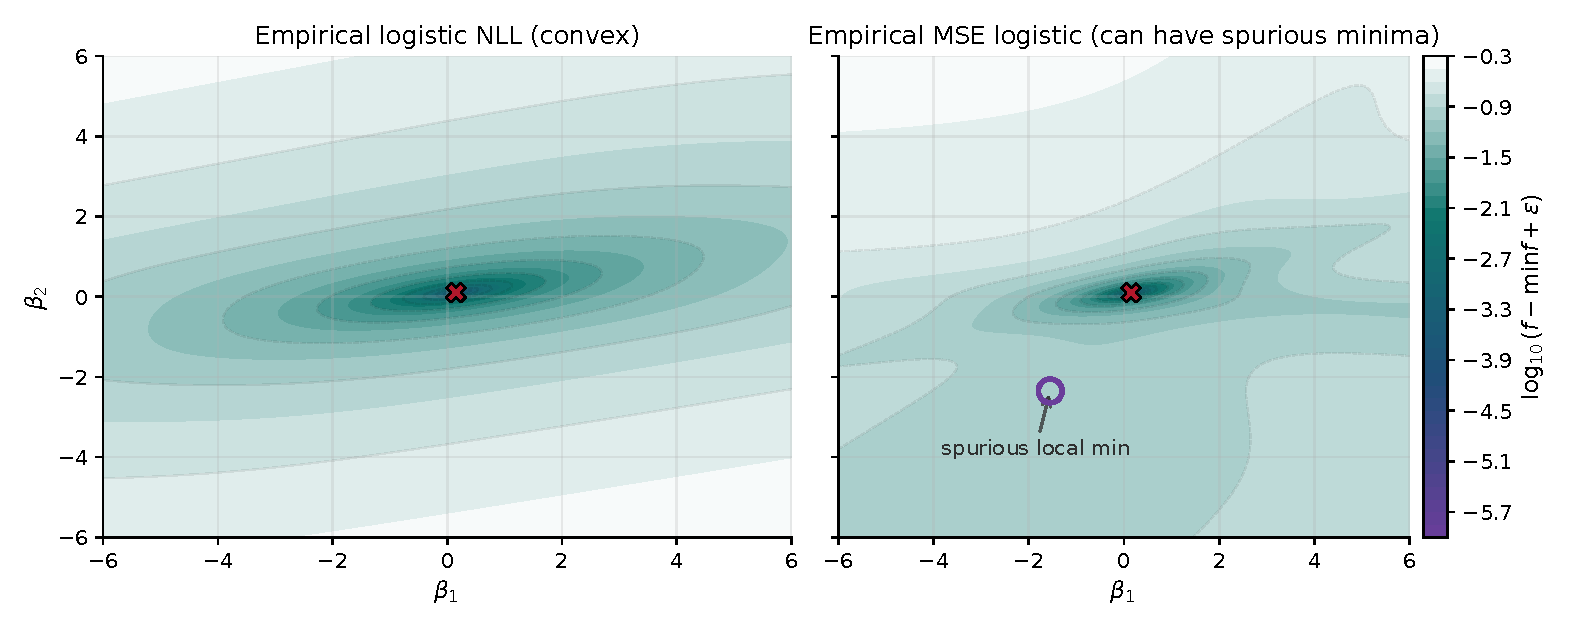
\includegraphics[width=\textwidth]{figures/handouts/convexity_optimization/fig_logistic_empirical_spurious}
  \caption{Empirical logistic landscapes on the dataset in \Cref{ex:logistic-empirical-spurious}.
  The plots show $\log_{10}(f-\min f+\varepsilon)$ for each objective.
  The red X marks the global minimizer in each panel.
  Left: the NLL is convex (one basin).
  Right: the squared-loss objective can have a spurious local minimum (circled), so a local method can get stuck.}
  \label{fig:logistic-empirical-spurious}
\end{figure}

\begin{figure}[t]
  \centering
  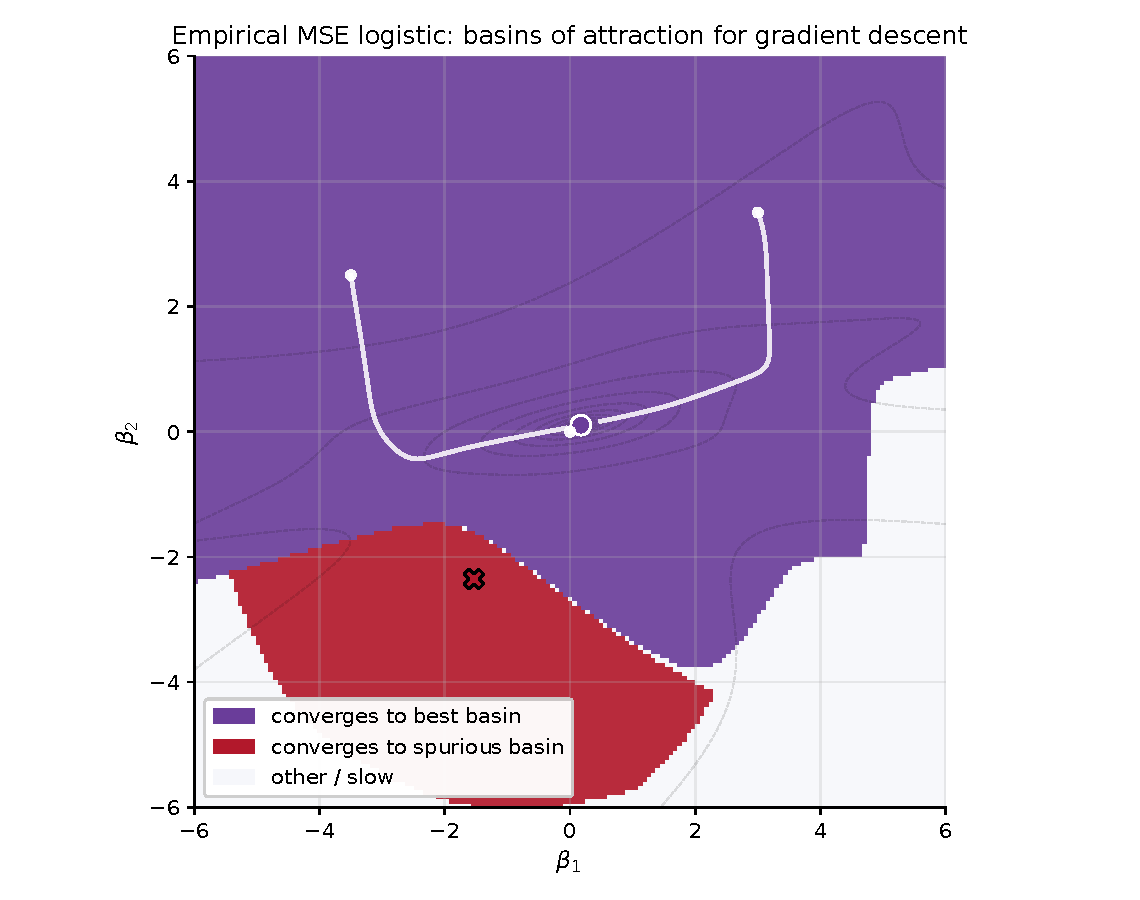
\includegraphics[width=0.92\textwidth]{figures/handouts/convexity_optimization/fig_logistic_empirical_basins}
  \caption{Basins of attraction for gradient descent on the empirical MSE-logistic objective in \Cref{ex:logistic-empirical-spurious}.
  The purple dot and red X mark the two local minimizers.
  Each initialization is colored by which local minimizer fixed-step GD (with $\eta=0.6$) converges to, and the overlaid paths show a few representative trajectories.}
  \label{fig:logistic-empirical-basins}
\end{figure}

Now assume a realizable population model:
\[
Y\mid X=x \sim \mathrm{Bernoulli}(p^\star(x)),
\qquad
p^\star(x) = \sigma(x^\top\beta^\star).
\]
Then the expected squared loss decomposes as
\[
\E\big[(Y-\sigma(X^\top\beta))^2\mid X\big]
= p^\star(X)(1-p^\star(X)) + \big(p^\star(X)-\sigma(X^\top\beta)\big)^2,
\]
so (up to an additive constant) the population objective becomes
\begin{equation}
R(\beta) = \E\big[(\sigma(X^\top\beta)-\sigma(X^\top\beta^\star))^2\big].
\label{eq:logistic-pop-risk}
\end{equation}

\begin{proposition}[One-point monotonicity in the realizable population squared-loss risk]
\label{prop:logistic-pop-one-point}
Assume $\E[\norm{X}_2]<\infty$, and let $R$ be as in \eqref{eq:logistic-pop-risk}. Then for all $\beta$,
\begin{equation}
\ip{\nabla R(\beta)}{\beta-\beta^\star} \ge 0.
\label{eq:one-point}
\end{equation}
In particular, along any ray $\beta(t)=\beta^\star+t(\beta-\beta^\star)$, the function $t\mapsto R(\beta(t))$ is nondecreasing for $t\ge 0$.
\end{proposition}

The next exercise isolates the population monotonicity calculation; structurally it plays the same role as the first-order convexity arguments in the Optimization unit.
\begin{exercise}[One-point monotonicity for realizable MSE-logistic]
\label{ex:logistic-one-point}
Prove \Cref{prop:logistic-pop-one-point}.
Let $\eta=X^\top\beta$ and $\eta^\star=X^\top\beta^\star$.
\begin{enumerate}[leftmargin=*]
  \item Differentiate under the expectation in \eqref{eq:logistic-pop-risk} to show that
  \[
  \nabla R(\beta)
  =2\,\E\Big[(\sigma(\eta)-\sigma(\eta^\star))\,\sigma'(\eta)\,X\Big].
  \]
  \item Show that
  \[
  \ip{\nabla R(\beta)}{\beta-\beta^\star}
  =2\,\E\Big[\sigma'(\eta)\,(\sigma(\eta)-\sigma(\eta^\star))(\eta-\eta^\star)\Big],
  \]
  and conclude it is nonnegative using only that $\sigma$ is increasing and $\sigma'\ge 0$.
  \item Deduce the ray-monotonicity statement by differentiating $g(t)=R(\beta^\star+t(\beta-\beta^\star))$.
\end{enumerate}
\end{exercise}

\SolutionBox[14]{%
\emph{Part (1).}
Differentiate \eqref{eq:logistic-pop-risk} under the expectation:
\[
R(\beta)=\E\big[(\sigma(X^\top\beta)-\sigma(X^\top\beta^\star))^2\big].
\]
Using the chain rule, $\nabla_\beta\sigma(X^\top\beta)=\sigma'(X^\top\beta)\,X$, hence
\[
\nabla R(\beta)
=2\,\E\Big[(\sigma(\eta)-\sigma(\eta^\star))\,\sigma'(\eta)\,X\Big],
\qquad
\eta=X^\top\beta,\ \eta^\star=X^\top\beta^\star.
\]

\emph{Part (2).}
Take the inner product with $(\beta-\beta^\star)$ and use $\ip{X}{\beta-\beta^\star}=\eta-\eta^\star$:
\[
\ip{\nabla R(\beta)}{\beta-\beta^\star}
=2\,\E\Big[\sigma'(\eta)\,(\sigma(\eta)-\sigma(\eta^\star))(\eta-\eta^\star)\Big].
\]
Since $\sigma'(\eta)\ge 0$ and $\sigma$ is increasing, we have
$(\sigma(\eta)-\sigma(\eta^\star))(\eta-\eta^\star)\ge 0$ pointwise.
Therefore the integrand is pointwise nonnegative, and the expectation is nonnegative as claimed.

\emph{Part (3) (ray monotonicity).}
For the ray $\beta(t)=\beta^\star+t(\beta-\beta^\star)$, define $g(t)=R(\beta(t))$.
By the chain rule,
\[
g'(t)=\ip{\nabla R(\beta(t))}{\beta-\beta^\star}\ge 0,
\]
so $t\mapsto R(\beta(t))$ is nondecreasing for $t\ge 0$.
(The argument uses only that the link is increasing with nonnegative derivative, so it holds for any such link function.)%
}

\begin{corollary}[Realizable population MSE-logistic has no spurious local minima]
\label{cor:logistic-pop-no-spurious}
Under the assumptions of \Cref{prop:logistic-pop-one-point}, every local minimizer of the realizable population risk $R$ in \eqref{eq:logistic-pop-risk} is global.
If in addition $\E[XX^\top]\succ 0$, then the unique global minimizer is $\beta^\star$.
\end{corollary}

\begin{exercise}[Stationarity + one-point monotonicity $\Rightarrow$ no spurious local minima]
\label{ex:logistic-one-point-no-spurious}
Prove \Cref{cor:logistic-pop-no-spurious} from \Cref{prop:logistic-pop-one-point}.
\begin{enumerate}[leftmargin=*]
  \item Let $\bar\beta$ be a local minimizer. Since $R$ is differentiable, $\nabla R(\bar\beta)=0$.
  Combine this with \Cref{eq:one-point} to show that
  \[
    0
    = \ip{\nabla R(\bar\beta)}{\bar\beta-\beta^\star}
    = 2\,\E\Big[\sigma'(\bar\eta)\,(\sigma(\bar\eta)-\sigma(\eta^\star))(\bar\eta-\eta^\star)\Big],
  \]
  where $\bar\eta=X^\top\bar\beta$ and $\eta^\star=X^\top\beta^\star$.
  Conclude that $\sigma(X^\top\bar\beta)=\sigma(X^\top\beta^\star)$ almost surely.
  \item Deduce that $R(\bar\beta)=0$, so $\bar\beta$ is a global minimizer.
  \item For uniqueness: show that if $R(\beta)=0$, then $X^\top(\beta-\beta^\star)=0$ almost surely, and deduce $\beta=\beta^\star$ under $\E[XX^\top]\succ 0$.
\end{enumerate}
\end{exercise}

\SolutionBox[14]{%
\emph{Part (1).}
Let $\bar\beta$ be a local minimizer of the differentiable function $R$.
Then $\nabla R(\bar\beta)=0$.
Applying \Cref{prop:logistic-pop-one-point} at $\beta=\bar\beta$ gives
\[
0
= \ip{\nabla R(\bar\beta)}{\bar\beta-\beta^\star}
= 2\,\E\Big[\sigma'(\bar\eta)\,(\sigma(\bar\eta)-\sigma(\eta^\star))(\bar\eta-\eta^\star)\Big],
\qquad \bar\eta=X^\top\bar\beta,\ \eta^\star=X^\top\beta^\star.
\]
The integrand is pointwise nonnegative because $\sigma'(\bar\eta)\ge 0$ and $\sigma$ is increasing, so the expectation can vanish only if the integrand is zero almost surely.
Since $\sigma'(z)>0$ for every finite $z$, this implies
\[
(\sigma(\bar\eta)-\sigma(\eta^\star))(\bar\eta-\eta^\star)=0
\qquad\text{almost surely.}
\]
Because $\sigma$ is strictly increasing, the product above is zero if and only if $\bar\eta=\eta^\star$, equivalently $\sigma(X^\top\bar\beta)=\sigma(X^\top\beta^\star)$ almost surely.

\emph{Part (2).}
If $\sigma(X^\top\bar\beta)=\sigma(X^\top\beta^\star)$ almost surely, then the integrand in \eqref{eq:logistic-pop-risk} vanishes almost surely, so
\[
R(\bar\beta)=\E\big[(\sigma(X^\top\bar\beta)-\sigma(X^\top\beta^\star))^2\big]=0.
\]
Since $R(\beta^\star)=0$ as well, $\bar\beta$ is a global minimizer.

\emph{Part (3) (uniqueness).}
If $R(\beta)=0$, then
\[
\E\big[(\sigma(X^\top\beta)-\sigma(X^\top\beta^\star))^2\big]=0,
\]
so $\sigma(X^\top\beta)=\sigma(X^\top\beta^\star)$ almost surely.
Since $\sigma$ is strictly increasing, this implies $X^\top(\beta-\beta^\star)=0$ almost surely.
Taking expectations yields
$(\beta-\beta^\star)^\top\E[XX^\top](\beta-\beta^\star)=0$.
If $\E[XX^\top]\succ 0$, then the quadratic form is strictly positive unless $\beta=\beta^\star$, so $\beta^\star$ is the unique global minimizer.%
}

The population MSE-logistic risk is nonconvex, but it still has the simple geometry that moving away from $\beta^\star$ does not help along any ray from $\beta^\star$.
This is qualitatively different from objectives like ecological logistic regression (\Cref{sec:ecological-logistic}), where aggregation introduces intrinsic nonconvexity and the landscape can have many distinct basins even under a clean population model.

Even with this benign global geometry, gradient descent can be slow because of saturation and flat plateaus.
The one-point monotonicity in \Cref{prop:logistic-pop-one-point} is a global geometry guarantee, but it is not a rate guarantee.
Far from $\beta^\star$, the squared-loss logistic objective can become very flat because the logistic link saturates:
$\sigma(z)\to 0$ or $1$ and $\sigma'(z)\to 0$ as $|z|\to\infty$.
The squared-loss gradient carries a factor of $\sigma'(X^\top\beta)$, so when the model is very confident (large $|X^\top\beta|$), the gradient can be tiny even if the objective value is not close to its minimum.
This mirrors the ``confidence weights'' story for convex NLL objectives:
in logistic NLL, curvature is largest near the decision boundary, while very confident points contribute little.
For squared loss, that same saturation suppresses the \emph{descent signal} itself, producing plateaus where $\norm{\nabla R(\beta)}_2$ is small even though $R(\beta)-R(\beta^\star)$ is not.

\begin{proposition}[Realizable squared-loss logistic: arbitrarily flat far from $\beta^\star$]
\label{prop:logistic-pop-flat}
Assume $\E[\norm{X}_2]<\infty$ and let $R$ be the realizable population risk \eqref{eq:logistic-pop-risk}.
Define $g(t)=R(t\beta^\star)$ for $t\ge 1$.
Then:
\begin{enumerate}[leftmargin=*]
  \item $g$ is nondecreasing on $[1,\infty)$ and converges to a finite limit $g(\infty)$.
  \item $\lim_{t\to\infty} g'(t)=0$ and $\lim_{t\to\infty}\norm{\nabla R(t\beta^\star)}_2=0$.
  \item If $\Pr(X^\top\beta^\star\neq 0)>0$, then $g(\infty)>0$.
\end{enumerate}
In particular, there are directions along which the landscape becomes arbitrarily flat even though the excess risk stays bounded away from $0$.
\end{proposition}

\emph{Proof idea.} See Exercise~\ref{ex:logistic-plateau}.

\begin{exercise}[Prove the plateau]
\label{ex:logistic-plateau}
In the realizable population model, let $g(t)=R(t\beta^\star)$ for $t\ge 1$.
\begin{enumerate}[leftmargin=*]
  \item Show that
  \[
    g'(t)=2\,\E\big[(\sigma(t\eta^\star)-\sigma(\eta^\star))\,\sigma'(t\eta^\star)\,\eta^\star\big],
    \qquad \eta^\star=X^\top\beta^\star,
  \]
  and conclude that $g$ is nondecreasing (hence $g(t)\to g(\infty)$ since $0\le g(t)\le 1$).
  \item Show that $g'(t)\to 0$ and $\nabla R(t\beta^\star)\to 0$ as $t\to\infty$.
  Interpret this as: \emph{without} a PL/strong-convexity-type condition, small gradient does not imply near-optimality.
  \item Assume $\Pr(\eta^\star\neq 0)>0$.
  Show that $g(\infty)>0$.
\end{enumerate}
\end{exercise}

\SolutionBox[12]{%
Write $\eta^\star=X^\top\beta^\star$ so that $g(t)=\E[(\sigma(t\eta^\star)-\sigma(\eta^\star))^2]$.

\emph{Part (1).}
Differentiate under the expectation:
by the chain rule,
\[
\frac{d}{dt}\sigma(t\eta^\star)=\sigma'(t\eta^\star)\,\eta^\star,
\]
so
\[
g'(t)
=\E\Big[2(\sigma(t\eta^\star)-\sigma(\eta^\star))\cdot \sigma'(t\eta^\star)\,\eta^\star\Big]
=2\,\E\big[(\sigma(t\eta^\star)-\sigma(\eta^\star))\,\sigma'(t\eta^\star)\,\eta^\star\big].
\]
For $t\ge 1$, $\sigma(t\eta^\star)-\sigma(\eta^\star)$ has the same sign as $(t-1)\eta^\star$ since $\sigma$ is increasing.
Because $\sigma'\ge 0$, the integrand is pointwise nonnegative, hence $g'(t)\ge 0$ and $g$ is nondecreasing.
Since $g(t)\in[0,1]$, it follows that $g(t)\to g(\infty)$ for some finite limit $g(\infty)$.

\emph{Part (2).}
For each fixed $\eta^\star\neq 0$, we have $t\eta^\star\to \pm\infty$ and therefore $\sigma'(t\eta^\star)\to 0$ as $t\to\infty$.
Also,
\[
\big|(\sigma(t\eta^\star)-\sigma(\eta^\star))\,\sigma'(t\eta^\star)\,\eta^\star\big|
\le \sigma'(0)\,|\eta^\star|
\le \sigma'(0)\,\norm{\beta^\star}_2\,\norm{X}_2,
\]
which is integrable since $\E[\norm{X}_2]<\infty$.
We will use the following standard fact: if random variables $Z_t$ satisfy $|Z_t|\le W$ with $\E[W]<\infty$ and $Z_t\to 0$ almost surely, then $\E[Z_t]\to 0$.
Applying this fact here gives $g'(t)\to 0$ as $t\to\infty$.

\smallskip
Similarly, differentiating \eqref{eq:logistic-pop-risk} gives
\[
\nabla R(t\beta^\star)
=2\,\E\big[(\sigma(t\eta^\star)-\sigma(\eta^\star))\,\sigma'(t\eta^\star)\,X\big].
\]
The integrand norm is bounded by $2\sigma'(0)\norm{X}_2$, and for each fixed $X$ the factor $\sigma'(t\eta^\star)$ tends to $0$ (or the bracketed term vanishes when $\eta^\star=0$), so the same reasoning lets us pass the limit through the expectation and conclude $\nabla R(t\beta^\star)\to 0$.

\emph{Part (3).}
As $t\to\infty$ we have $\sigma(t\eta^\star)\to 1$ when $\eta^\star>0$, $\sigma(t\eta^\star)\to 0$ when $\eta^\star<0$, and $\sigma(t\eta^\star)=\sigma(\eta^\star)=1/2$ when $\eta^\star=0$.
Since $0\le (\sigma(t\eta^\star)-\sigma(\eta^\star))^2\le 1$, we can apply the same fact (with $W=1$) to pass the limit through the expectation and obtain
\[
g(\infty)=\E\Big[(1-\sigma(\eta^\star))^2\mathbf{1}\{\eta^\star>0\} + \sigma(\eta^\star)^2\mathbf{1}\{\eta^\star<0\}\Big].
\]
If $\Pr(\eta^\star\neq 0)>0$, then the integrand is strictly positive on $\{\eta^\star\neq 0\}$, so $g(\infty)>0$.

Along this ray, the risk can remain bounded away from $0$ while the gradient (and directional derivative) goes to $0$.
Without a condition like PL/strong convexity, a small gradient does not by itself certify near-optimality.
}

Conditions like strong convexity or the PL inequality (\Cref{def:pl-inequality}) prevent this phenomenon: they rule out large flat regions away from the optimum by relating gradient size to suboptimality.
\Cref{prop:logistic-pop-flat} shows the realizable squared-loss logistic risk does not have such a global guarantee in general.

In the realizable population model, the one-point monotonicity in \Cref{prop:logistic-pop-one-point} is a \emph{global} geometric statement.
To get an actual rate for gradient descent, we also need a \emph{local curvature} condition near $\beta^\star$.
One simple sufficient condition is bounded features, which implies local strong convexity (hence a linear rate) around the optimum.

\begin{proposition}[Local linear convergence of gradient descent near $\beta^\star$]
\label{prop:logistic-pop-local-rate}
Assume $\E[XX^\top]\succeq \lambda I_d$ and $\norm{X}_2\le R$ almost surely for some $\lambda,R>0$.
Then at $\beta^\star$,
\[
\Hess R(\beta^\star)\succeq m_0 I_d,
\qquad
m_0 = 2\,\sigma'(R\norm{\beta^\star}_2)^2\,\lambda,
\]
and there exist $r>0$ and constants $0<m\le L<\infty$ such that the population risk $R$ in \eqref{eq:logistic-pop-risk} is $m$-strongly convex and $L$-smooth on the ball $\{\beta:\ \norm{\beta-\beta^\star}_2\le r\}$.
Consequently, gradient descent with step size $1/L$ initialized in this ball satisfies
\[
R(\beta^{(k)})-R(\beta^\star)
\le \left(1-\frac{m}{L}\right)^k\bigl(R(\beta^{(0)})-R(\beta^\star)\bigr)
\qquad\text{(see \citealp[\S9.3]{boyd_vandenberghe_2004_convex}).}
\]
\end{proposition}

\begin{proof}
Differentiate \eqref{eq:logistic-pop-risk} twice.
At $\beta=\beta^\star$, the cross term vanishes and the Hessian simplifies to
\[
\Hess R(\beta^\star)=2\,\E\big[\sigma'(X^\top\beta^\star)^2\,XX^\top\big].
\]
Since $\norm{X^\top\beta^\star}\le \norm{X}_2\norm{\beta^\star}_2\le R\norm{\beta^\star}_2$ almost surely, we have
$\sigma'(X^\top\beta^\star)\ge \sigma'(R\norm{\beta^\star}_2)>0$ almost surely (since $\sigma'$ is even and decreases with $|z|$), hence
\[
\Hess R(\beta^\star)\succeq 2\,\sigma'(R\norm{\beta^\star}_2)^2\,\E[XX^\top]\succeq 2\,\sigma'(R\norm{\beta^\star}_2)^2\,\lambda I_d.
\]
This is the claimed bound with $m_0=2\,\sigma'(R\norm{\beta^\star}_2)^2\,\lambda$.
Because $R$ is twice continuously differentiable and $\norm{X}_2\le R$ almost surely, $\Hess R(\beta)$ varies continuously in $\beta$ and is bounded on compact sets.
Therefore, on a sufficiently small ball around $\beta^\star$, the Hessian is bounded below by (say) $\tfrac12 m_0 I_d$ and above by $L I_d$ for some finite $L$, which gives local strong convexity and smoothness.
The linear convergence rate for gradient descent on an $m$-strongly convex and $L$-smooth function is standard (cited above).
\end{proof}

Under misspecification, hard multimodality can return.
If $p^\star(x)$ is not representable as $\sigma(x^\top\beta)$ (e.g.\ marginalizing over latent classes can yield mixtures of logits), then \eqref{eq:one-point} need not hold, and the population squared-loss risk can become bimodal with spurious local minima.
Benign global geometry often hinges on model and data assumptions.
This is one reason MLE (convex NLL) is often more stable than squared-loss fitting in logistic-type binary regression models.

\begin{example}[Misspecification can create a spurious local minimum for squared-loss logistic regression]
\label{ex:logistic-misspecified-spurious}
Consider a 1D feature $X$ that takes values $\{-2,-1,1,2\}$ with equal probability, and parameterize $\beta=(\beta_0,\beta_1)$ so that $q_\beta(x)=\sigma(\beta_0+\beta_1 x)$.
Let the true conditional probabilities be
\[
p^\star(-2)=0.49,\quad p^\star(-1)=0.87,\quad p^\star(1)=0.92,\quad p^\star(2)=0.36.
\]
This $p^\star$ is not representable as $q_\beta$, since it is not monotone in $x$.

For the population squared-loss risk $R_{\mathrm{MSE}}(\beta)=\E[(q_\beta(X)-p^\star(X))^2]$, a direct evaluation shows two distinct basins:
numerically, evaluating $R_{\mathrm{MSE}}$ on a grid reveals a global minimizer and a spurious local minimizer.
See \Cref{fig:logistic-landscape-2d}.
\end{example}

\begin{figure}[t]
  \centering
  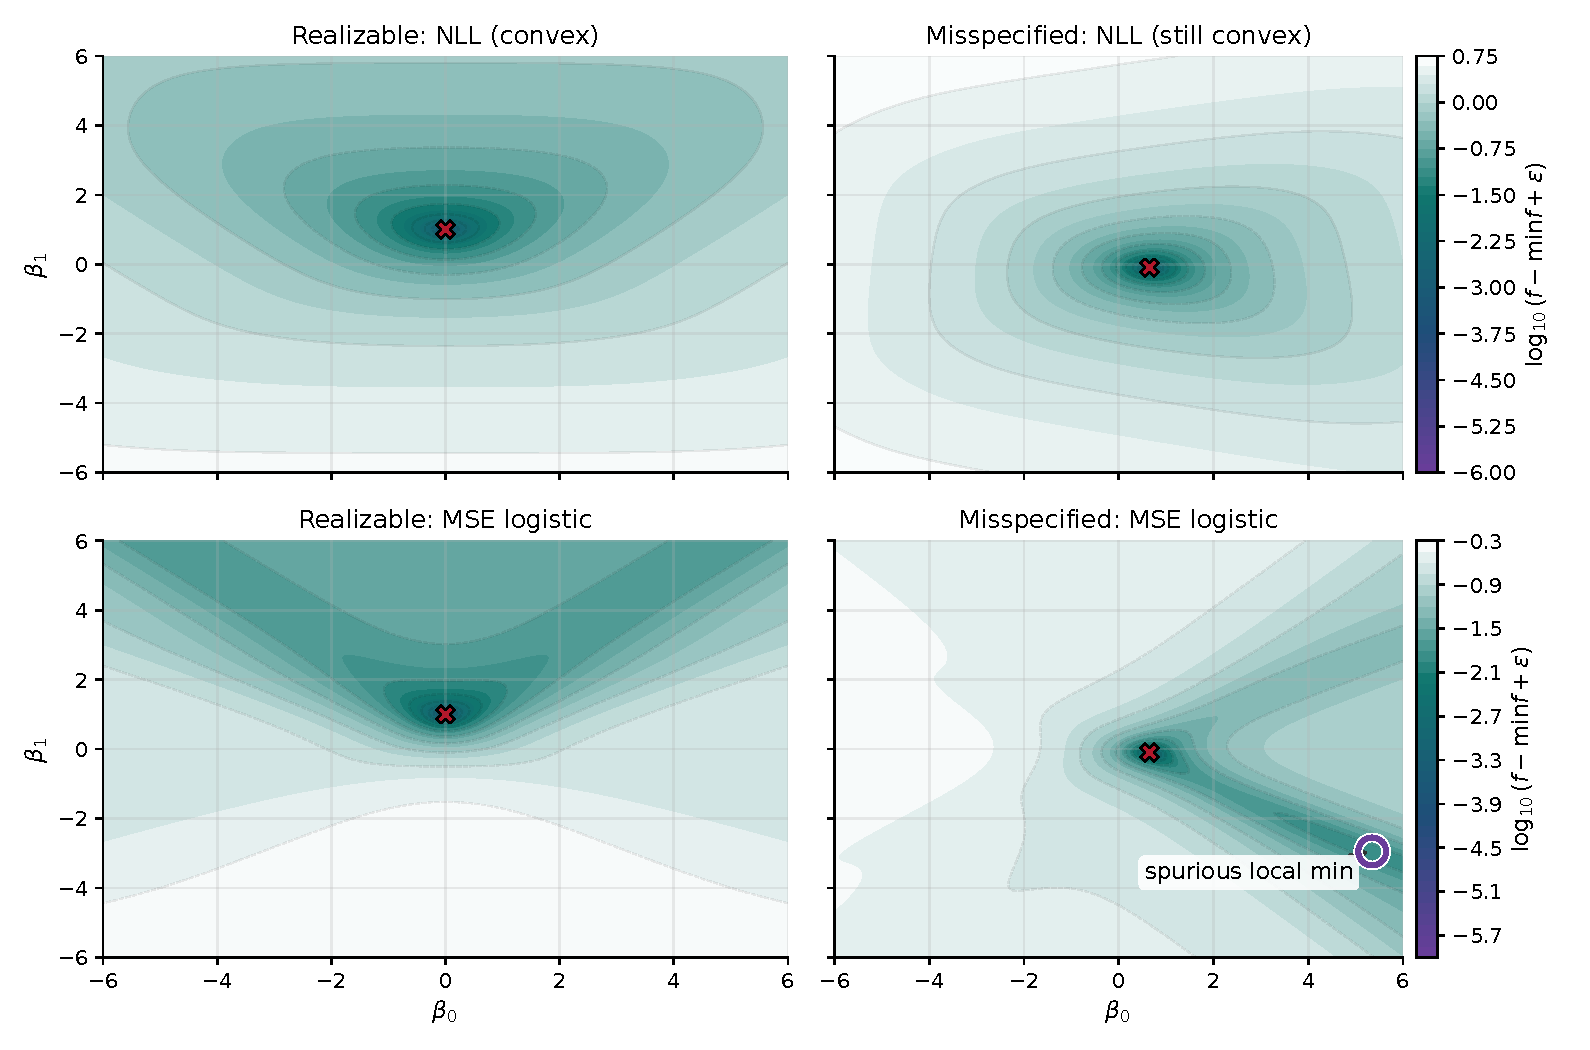
\includegraphics[width=\textwidth]{figures/handouts/convexity_optimization/fig_logistic_landscape_2d}
  \caption{A consistent contourf view of logistic landscapes in a 2D parameterization $\beta=(\beta_0,\beta_1)$.
  The plots show $\log_{10}(f-\min f+\varepsilon)$ for each objective, which makes basins comparable across panels.
  The red X marker indicates the global minimizer in each panel; in the bottom-right plot, the circled point is a spurious local minimum.
  In this example, the NLL landscape is unimodal in both realizable and misspecified settings, while the squared-loss landscape can develop extra basins under misspecification.}
  \label{fig:logistic-landscape-2d}
\end{figure}

% ------------------------------------------------------------
Example~I separates three distinct regimes.
Empirical MSE-logistic can create spurious basins; the realizable population risk has no spurious local minima but can still be slow because of broad plateaus; and misspecification can bring back genuinely wrong stable basins.
The response depends on the regime: use a stable objective when possible, use damping or line search when curvature is unreliable, and use restarts or stronger initializations when multiple basins are present.

% ------------------------------------------------------------
\section[Example II (phase retrieval)]{Example II: multimodality from symmetry, but only global optima in phase retrieval}
\label{sec:phase-retrieval}

In coherent diffraction imaging, optics, and astronomy, sensors measure intensities and lose phase.
A canonical real model is \emph{phase retrieval}:
\[
y_i = (a_i^\top x^\star)^2,\qquad i=1,\dots,m,
\]
where $x^\star\in\R^d$ is the unknown signal and $a_i$ are known sensing vectors.
A standard nonconvex least-squares objective is
\begin{equation}
F(x)=\frac{1}{4m}\sum_{i=1}^m\big((a_i^\top x)^2 - y_i\big)^2.
\label{eq:phase-empirical}
\end{equation}
This objective is nonconvex for structural reasons (it involves squares of linear forms),
and it is \emph{inherently} multimodal because $x^\star$ and $-x^\star$ generate the same data.

Like squared-loss logistic regression, phase retrieval is a smooth, nonconvex least-squares objective.
But here the nonconvexity is driven primarily by a \emph{symmetry}: $x^\star$ and $-x^\star$ generate the same data.
In population (for Gaussian designs), this symmetry produces multiple global optima but \emph{no} suboptimal local minima; the remaining stationary points are saddles.
This is ``benign'' nonconvexity (a strict-saddle picture), and it contrasts with ecological logistic regression (\Cref{sec:ecological-logistic}), where aggregation creates intrinsic nonconvexity and can lead to many distinct basins.
This ``benign geometry'' picture (multiple equivalent global minimizers; strict saddles elsewhere) appears broadly in modern tractable nonconvex problems; see \citet[\S2]{sun_qu_wright_2015_nonconvex_not_scary} and \citet[\S1]{zhang_qu_wright_2020_symmetry_geometry}.

\begin{figure}[t]
  \centering
  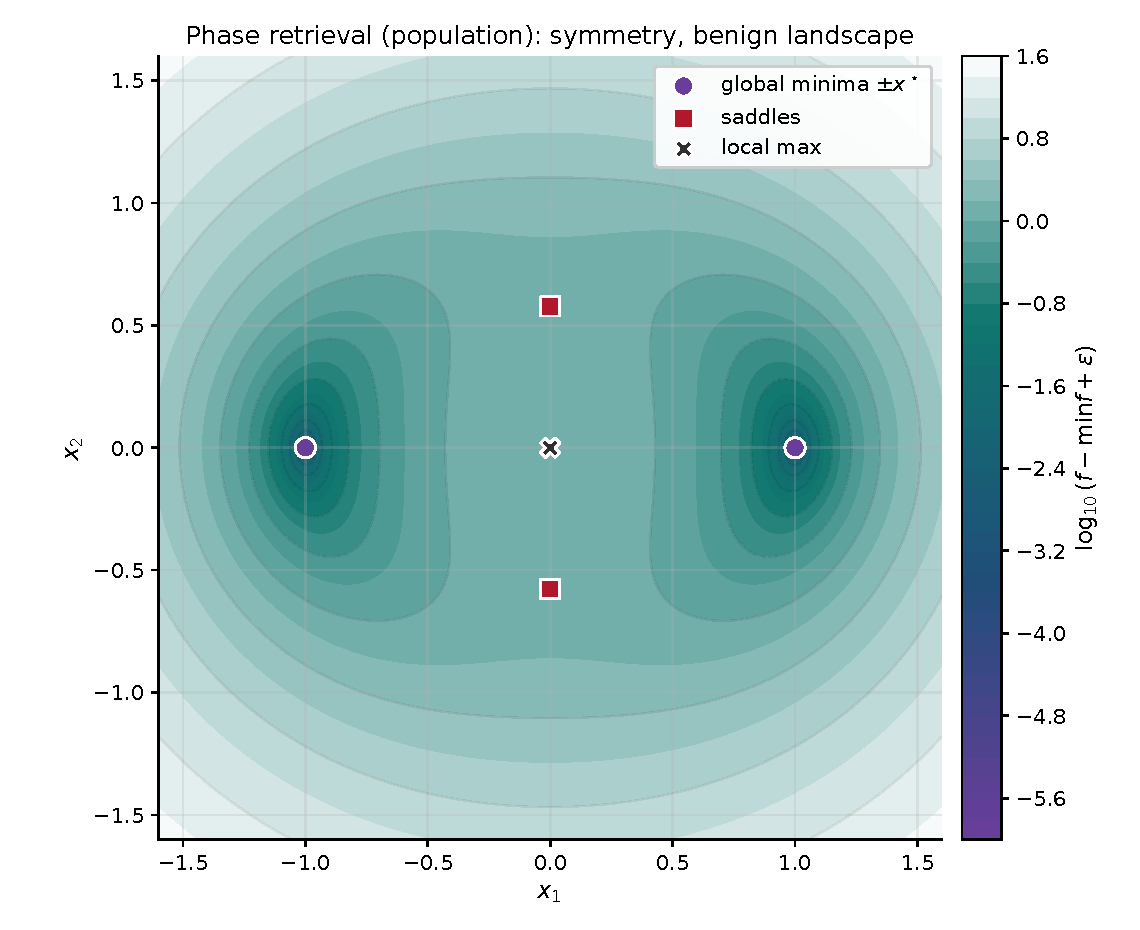
\includegraphics[width=0.86\textwidth]{figures/handouts/convexity_optimization/fig_phase_retrieval_landscape}
  \caption{Population phase retrieval in $d=2$: the landscape is nonconvex and symmetric ($x\sim -x$), but the only local minima are the two global minima $\pm x^\star$; other critical points are saddles or a local maximum at the origin.}
  \label{fig:phase-retrieval-landscape}
\end{figure}

For a clean population model, assume $a\sim N(0,I_d)$ and consider the \emph{population} objective
\begin{equation}
  f(x)=\frac12\,\E\Big[\big((a^\top x)^2 - (a^\top x^\star)^2\big)^2\Big].
  \label{eq:phase-pop}
\end{equation}

\begin{proposition}[Population phase retrieval: nonconvex but no spurious local minima]
\label{prop:phase-retrieval-benign}
For $f$ in \eqref{eq:phase-pop},
\begin{equation}
  f(x)
  =\frac{3}{2}\norm{x}^4 - \norm{x}^2\norm{x^\star}^2 - 2\ip{x}{x^\star}^2 + \frac{3}{2}\norm{x^\star}^4,
  \label{eq:phase-pop-closed-form}
\end{equation}
and the stationary points are:
\begin{enumerate}[leftmargin=*]
  \item global minima $x=\pm x^\star$ (value $0$),
  \item a local maximum at $x=0$,
  \item a saddle set $\{x:\ x\perp x^\star,\ \norm{x}=\norm{x^\star}/\sqrt{3}\}$.
\end{enumerate}
In particular, every local minimum is global.
\end{proposition}

\begin{exercise}[Phase retrieval: derive and classify the population stationary points]
\label{ex:phase-pop-derivation}
Prove \Cref{prop:phase-retrieval-benign}.
\begin{enumerate}[leftmargin=*]
  \item Expand \eqref{eq:phase-pop} and use the Gaussian fourth-moment identities
  \[
  \E[(a^\top u)^4]=3\norm{u}^4,
  \qquad
  \E[(a^\top u)^2(a^\top v)^2]=\norm{u}^2\norm{v}^2 + 2\ip{u}{v}^2,
  \]
  to obtain \eqref{eq:phase-pop-closed-form}.
  \item Differentiate \eqref{eq:phase-pop-closed-form} to get an explicit formula for $\nabla f(x)$.
  \item Solve $\nabla f(x)=0$ by decomposing $x=\alpha x^\star + u$ with $u\perp x^\star$.
  \item Classify the stationary points as global minima, a local maximum, and a saddle set.
\end{enumerate}
\end{exercise}

\SolutionBox[22]{%
\emph{Part (1) (closed form).}
Expanding the square in \eqref{eq:phase-pop} gives
\[
f(x)
=\frac12\,\E\big[(a^\top x)^4\big]
\;-\;\E\big[(a^\top x)^2(a^\top x^\star)^2\big]
\;+\;\frac12\,\E\big[(a^\top x^\star)^4\big].
\]
Apply the stated Gaussian fourth-moment identities with $u=x$ and $v=x^\star$ to get
\[
\E[(a^\top x)^4]=3\norm{x}^4,\qquad
\E[(a^\top x^\star)^4]=3\norm{x^\star}^4,
\]
and
\[
\E[(a^\top x)^2(a^\top x^\star)^2]=\norm{x}^2\norm{x^\star}^2 + 2\ip{x}{x^\star}^2.
\]
Substituting yields \eqref{eq:phase-pop-closed-form}.

\emph{Part (2) (gradient).}
Differentiate \eqref{eq:phase-pop-closed-form}:
\[
\nabla f(x)
= 6\norm{x}^2 x - 2\norm{x^\star}^2 x - 4\ip{x}{x^\star}x^\star
= (6\norm{x}^2-2\norm{x^\star}^2)x - 4\ip{x}{x^\star}x^\star.
\]

\emph{Part (3) (stationary points).}
Let $r=\norm{x^\star}_2$ and decompose $x=\alpha x^\star + u$ with $u\perp x^\star$.
Then $\ip{x}{x^\star}=\alpha r^2$ and $\norm{x}^2=\alpha^2r^2+\norm{u}^2$.
Setting $\nabla f(x)=0$ and matching the $u$ and $x^\star$ components gives
\[
(6\norm{x}^2-2r^2)\,u=0,
\qquad
\alpha\,(6\norm{x}^2-6r^2)=0.
\]
If $u=0$, then either $\alpha=0$ (so $x=0$) or $\norm{x}^2=r^2$ (so $\alpha=\pm 1$ and $x=\pm x^\star$).
If $u\neq 0$, then the first equation forces $\norm{x}^2=r^2/3$, and the second forces $\alpha=0$, hence
$x\perp x^\star$ and $\norm{x}=r/\sqrt{3}$.
This gives exactly the stationary-point list in \Cref{prop:phase-retrieval-benign}.

\emph{Part (4) (classification).}
Since $f$ in \eqref{eq:phase-pop} is an expectation of a square, $f(x)\ge 0$ for all $x$.
Also $f(\pm x^\star)=0$, so $\pm x^\star$ are global minima.

For $x=0$, the expansion \eqref{eq:phase-pop-closed-form} shows
\[
f(0)-f(x)= r^2\norm{x}^2 + 2\ip{x}{x^\star}^2 - \frac{3}{2}\norm{x}^4,
\]
which is strictly positive for all sufficiently small $x\neq 0$ (the quadratic term dominates), so $x=0$ is a local maximum.

Finally, if $x\perp x^\star$ and $\norm{x}=r/\sqrt{3}$, then the univariate restriction $t\mapsto f(x+t x^\star)$ has negative second derivative at $t=0$, so there is a direction of negative curvature.
Hence these points are saddles, and every local minimum is global.%
}

This is symmetry-driven nonconvexity with a strict-saddle geometry:
every non-optimal stationary point has a direction of negative curvature.

Phase retrieval is typically approached via the two-stage template in \Cref{alg:two-stage-template}:
use a cheap global initializer, then run a local method.
In the Gaussian model, there is a clean way to build a provably good direction estimate from a simple moment identity.
Assume the noiseless Gaussian design model $a_i \stackrel{\mathrm{iid}}{\sim} N(0,I_d)$ with measurements $y_i=(a_i^\top x^\star)^2$.
Define the \emph{spectral matrix}
\[
  Y = \frac{1}{m}\sum_{i=1}^m y_i a_i a_i^\top.
\]
Also define the radius estimate
\[
  \hat r^2 = \frac{1}{m}\sum_{i=1}^m y_i,
\]
which satisfies $\E[\hat r^2]=\norm{x^\star}_2^2$.
If $\hat u$ is a unit-norm top eigenvector of $Y$, then the standard spectral initializer is $x^{(0)}=\hat r\,\hat u$.

The next proposition explains why this initialization is reasonable.
It shows that (i) the population matrix $\E[Y]$ has a unique leading eigenvector in the $x^\star$ direction, and (ii) if the empirical $Y$ is close to $\E[Y]$ in operator norm then its leading eigenvector must be close to $\pm x^\star/\norm{x^\star}_2$.
(Here $\norm{M}_{\mathrm{op}}$ denotes the operator norm, i.e.\ the largest absolute eigenvalue for a symmetric matrix $M$.)

\begin{proposition}[Gaussian phase retrieval: why the spectral initializer points at $x^\star$]
\label{prop:phase-spectral-init}
Assume $x^\star\neq 0$, let $a\sim N(0,I_d)$, and set $y=(a^\top x^\star)^2$.
Write $r=\norm{x^\star}_2$ and $u^\star=x^\star/r$.
Define the population matrix
\[
  Y_{\mathrm{pop}} = \E\big[y\,a a^\top\big]
  = \E\big[(a^\top x^\star)^2 a a^\top\big].
\]
Then
\[
  Y_{\mathrm{pop}}=r^2 I_d + 2x^\star(x^\star)^\top,
\]
so the unique leading eigenvector of $Y_{\mathrm{pop}}$ is $u^\star$.
Moreover, if $Y$ is any symmetric matrix satisfying
\[
\norm{Y-Y_{\mathrm{pop}}}_{\mathrm{op}} \le \varepsilon\, r^2
\qquad\text{for some }\varepsilon\in(0,1),
\]
then for every unit-norm leading eigenvector $\hat u$ of $Y$ there exists a sign $s\in\{\pm 1\}$ such that
$\norm{\hat u-su^\star}_2\le \sqrt{2\varepsilon}$.
\end{proposition}

\begin{exercise}[Phase retrieval: why spectral initialization points at $x^\star$]
\label{ex:phase-spectral-spike}
Prove \Cref{prop:phase-spectral-init}.
Conclude that if the empirical matrix $Y$ is close to $Y_{\mathrm{pop}}$ in operator norm, then its top eigenvector is close to $\pm u^\star$ and the spectral initializer $x^{(0)}=\hat r\,\hat u$ is close to $\pm x^\star$.
\emph{Hint:} to compute $Y_{\mathrm{pop}}$, you can either compute entries using the Gaussian fourth-moment identity
$\E[a_i a_j a_k a_\ell]=\delta_{ij}\delta_{k\ell}+\delta_{ik}\delta_{j\ell}+\delta_{i\ell}\delta_{jk}$,
or compute the entries directly by expanding.
For the perturbation bound, compare quadratic forms $v^\top Y v$ and use $|v^\top (Y-Y_{\mathrm{pop}}) v|\le \norm{Y-Y_{\mathrm{pop}}}_{\mathrm{op}}$ for unit $v$.
Finally, explain in a sentence why one expects $\norm{Y-Y_{\mathrm{pop}}}_{\mathrm{op}}$ to be small when $m$ is large in the Gaussian model.
\end{exercise}

\SolutionBox[20]{%
Write $u=x^\star$ and expand $y=(a^\top u)^2=\sum_{k,\ell} u_k u_\ell a_k a_\ell$.
For each entry $(i,j)$,
\[
\E\!\big[y\,a_i a_j\big]
=\sum_{k,\ell} u_k u_\ell\,\E[a_i a_j a_k a_\ell]
=\sum_{k,\ell} u_k u_\ell\bigl(\delta_{ij}\delta_{k\ell}+\delta_{ik}\delta_{j\ell}+\delta_{i\ell}\delta_{jk}\bigr).
\]
The first term gives $\delta_{ij}\sum_k u_k^2=\delta_{ij}\norm{u}_2^2$.
The second and third terms each give $u_i u_j$.
Thus $\E[y\,a_i a_j]=\norm{u}_2^2\,\delta_{ij}+2u_i u_j$, i.e.
$Y_{\mathrm{pop}}=\norm{u}_2^2 I_d + 2uu^\top$.

For eigenvalues, note that $Y_{\mathrm{pop}}u=(\norm{u}_2^2+2\norm{u}_2^2)u=3\norm{u}_2^2 u$.
If $w\perp u$, then $uu^\top w=0$ so $Y_{\mathrm{pop}}w=\norm{u}_2^2 w$.
Hence the unique top eigenspace is $\mathrm{span}\{u\}$.

Let $r=\norm{u}_2$ and $u^\star=u/r$.
Let $\hat u$ be a unit top eigenvector of $Y$.
Write $E=Y-Y_{\mathrm{pop}}$ and assume $\norm{E}_{\mathrm{op}}\le \varepsilon r^2$.
Then
\[
\hat u^\top Y_{\mathrm{pop}} \hat u
= \hat u^\top Y \hat u - \hat u^\top E \hat u
\ge \lambda_{\max}(Y) - \norm{E}_{\mathrm{op}}
\ge (u^\star)^\top Y u^\star - \norm{E}_{\mathrm{op}}
\ge 3r^2 - 2\varepsilon r^2.
\]
On the other hand,
$
\hat u^\top Y_{\mathrm{pop}} \hat u
= r^2 + 2r^2\,|\ip{\hat u}{u^\star}|^2.
$
Combining gives $|\ip{\hat u}{u^\star}|^2\ge 1-\varepsilon$.
Choosing the sign that maximizes the inner product,
\[
\min\{\norm{\hat u-u^\star}_2,\norm{\hat u+u^\star}_2\}^2
=2\bigl(1-|\ip{\hat u}{u^\star}|\bigr)
\le 2\bigl(1-|\ip{\hat u}{u^\star}|^2\bigr)
\le 2\varepsilon.
\]

The matrix $Y$ is an empirical average of i.i.d.\ symmetric matrices with mean $Y_{\mathrm{pop}}$.
To make this quantitative in high dimensions, one uses concentration inequalities for random matrices to bound $\norm{Y-Y_{\mathrm{pop}}}_{\mathrm{op}}$ with high probability; see \citet[\S2.2]{zhang_qu_wright_2020_symmetry_geometry} for discussion and references.
These probability tools are largely orthogonal to our focus here.%
}

Once you have an initialization that is close to $\pm x^\star$, the local stage behaves like the convex story again.
In the Gaussian population objective, $\pm x^\star$ are not only global minima: they are \emph{locally strongly convex} minima, so the standard local strong-convexity analysis from the Optimization unit gives a linear rate while the iterates remain in that neighborhood.

\begin{exercise}[Phase retrieval: local convexity near $\pm x^\star$ in the population objective]
\label{ex:phase-pop-local-strong-convex}
For the population objective $f$ in \eqref{eq:phase-pop-closed-form}, compute the Hessian $\Hess f(x)$ and show that
\[
\Hess f(x^\star)=4\norm{x^\star}_2^2 I_d + 8x^\star(x^\star)^\top.
\]
Deduce the eigenvalues of $\Hess f(x^\star)$ and interpret this as a local condition-number statement near $x^\star$.
\end{exercise}

\SolutionBox[12]{%
Differentiate the gradient formula in the solution to \Cref{ex:phase-pop-derivation}:
for $x\in\R^d$,
\[
\Hess f(x)=12xx^\top + (6\norm{x}_2^2-2\norm{x^\star}_2^2)I_d - 4x^\star(x^\star)^\top.
\]
At $x=x^\star$ this becomes
\[
\Hess f(x^\star)=(12-4)x^\star(x^\star)^\top + 4\norm{x^\star}_2^2 I_d
=8x^\star(x^\star)^\top + 4\norm{x^\star}_2^2 I_d.
\]
Along $u^\star=x^\star/\norm{x^\star}_2$ the eigenvalue is $12\norm{x^\star}_2^2$, and along any direction orthogonal to $x^\star$ the eigenvalue is $4\norm{x^\star}_2^2$.
So near $x^\star$ the population objective is well conditioned (local condition number $3$), which is exactly the regime where local methods behave like in the convex case.%
}

These pieces give the standard Gaussian-model story:
spectral initialization supplies a direction close to $\pm x^\star$, and the local geometry near $\pm x^\star$ is strongly convex, so local methods converge quickly once initialized there.
Rigorous finite-sample analyses follow this template; see \citet[\S2.2]{zhang_qu_wright_2020_symmetry_geometry} and references therein.

Phase retrieval shows a different kind of nonconvexity.
The sign symmetry creates multiple optima, but they are equivalent, and the remaining stationary points are saddles rather than bad local minima.
The right response is therefore not exhaustive global search; it is a coarse initializer, such as a spectral method, followed by local refinement inside the basin of $\pm x^\star$.



% ------------------------------------------------------------
\section[Example III (ecological logistic)]{Example III: hard nonconvexity from aggregation in ecological logistic regression}
\label{sec:ecological-logistic}

In some applications we observe covariates at the unit level but only aggregated outcomes.
For example, we might see covariates $x_{g,1},\dots,x_{g,n_g}$ for individuals in a group (a precinct, a cohort, a batch),
but instead of observing the binary outcomes $Y_{g,i}\in\{0,1\}$ we only observe the group total
\[
Z_g = \sum_{i=1}^{n_g} Y_{g,i}.
\]
Many different binary vectors $(Y_{g,1},\dots,Y_{g,n_g})$ can produce the same total $Z_g$, so the likelihood for $\beta$ must marginalize over a large discrete set of latent ``assignments.''

Assume a logistic model at the unit level:
\[
\Pr(Y_{g,i}=1\mid x_{g,i},\beta)=\sigma(x_{g,i}^\top\beta),
\qquad i=1,\dots,n_g,
\]
with conditional independence across $i$ given the covariates.
Write $p_{g,i}(\beta)=\sigma(x_{g,i}^\top\beta)$.
Then $Z_g$ is a sum of independent but non-identically distributed Bernoulli random variables (a Poisson--binomial model), and the marginal likelihood contains $\binom{n_g}{z_g}$ terms.
The resulting negative log-likelihood is typically nonconvex in $\beta$.
This combinatorial marginalization also creates a separate difficulty that is easy to miss if we focus only on the geometry:
when $n_g$ is large, the likelihood term $\Pr(Z_g=z_g\mid x_{g,1},\dots,x_{g,n_g},\beta)$ can be expensive to evaluate repeatedly inside an optimizer.
The naive computation is literally a sum over $\binom{n_g}{z_g}$ assignments (as in \Cref{ex:eco-logistic-nonconvex}), which is intractable for large groups.
This ``optimization + marginalization'' pattern is common in latent-variable models: hard landscapes and expensive objective evaluations can come together.

An empirical negative log-likelihood objective for $G$ independent groups is
\begin{equation}
  f(\beta)
  =
  -\frac{1}{G}\sum_{g=1}^G \log \Pr(Z_g=z_g \mid x_{g,1},\dots,x_{g,n_g},\beta).
  \label{eq:eco-logistic-obj}
\end{equation}
Two edge cases are instructive.
In the special case where the covariates are constant within each group ($x_{g,i}\equiv x_g$), we have
$Z_g\sim \mathrm{Binomial}(n_g,\sigma(x_g^\top\beta))$, and \eqref{eq:eco-logistic-obj} reduces to the usual convex binomial logistic-regression objective from the Optimization unit.
At the other extreme, if $d=1$ with $\beta=(\beta_0,\beta_1)$ and each group contains covariates in $\pm$ pairs (for every $x$ the value $-x$ appears with the same multiplicity), then the marginal likelihood is symmetric in the slope: it is unchanged under $\beta_1\mapsto -\beta_1$.
This kind of symmetry reflects a genuine non-identifiability from totals alone.

\begin{exercise}[Ecological logistic regression: two easy special cases]
\label{ex:eco-logistic-edge-cases}
\begin{enumerate}[leftmargin=*]
  \item Suppose $x_{g,i}\equiv x_g$ within each group.
  Show that $Z_g\sim \mathrm{Binomial}(n_g,\sigma(x_g^\top\beta))$ and conclude that the corresponding negative log-likelihood is convex in $\beta$.
  \item Assume $d=1$ with $\beta=(\beta_0,\beta_1)$ and suppose the multiset $\{x_1,\dots,x_n\}$ is symmetric: for every $x$ it contains $-x$ with the same multiplicity.
  Show that, for every $z$,
  \[
    \Pr(Z=z\mid x_1,\dots,x_n,(\beta_0,\beta_1))
    =
    \Pr(Z=z\mid x_1,\dots,x_n,(\beta_0,-\beta_1)).
  \]
  Conclude that the likelihood for $\beta_1$ is an even function, so the sign of the slope is not identifiable from $Z$ alone in such a balanced design.
\end{enumerate}
\end{exercise}

\SolutionBox[14]{%
\emph{Part (1).}
If $x_{g,i}\equiv x_g$, then conditional on $x_g$ the unit-level outcomes are i.i.d.\ Bernoulli with success probability $\sigma(x_g^\top\beta)$.
Therefore $Z_g=\sum_{i=1}^{n_g}Y_{g,i}\sim \mathrm{Binomial}(n_g,\sigma(x_g^\top\beta))$.
Up to an additive constant (independent of $\beta$), the per-group negative log-likelihood can be written as a function of the scalar $\eta=x_g^\top\beta$:
\[
\ell_g(\beta)
= -z_g\,\eta + n_g\log(1+e^\eta).
\]
Since $\frac{d^2}{d\eta^2}\ell_g(\eta)=n_g\,\sigma'(\eta)\ge 0$, the map $\eta\mapsto \ell_g(\eta)$ is convex.
Composing a convex function with a linear map $\beta\mapsto x_g^\top\beta$ preserves convexity, so $\ell_g$ is convex in $\beta$.
Summing over $g$ preserves convexity, hence the full objective is convex.

\emph{Part (2).}
Write $p_i(\beta_0,\beta_1)=\sigma(\beta_0+\beta_1 x_i)$.
Replacing $\beta_1$ by $-\beta_1$ replaces $p_i$ by $\tilde p_i=\sigma(\beta_0-\beta_1 x_i)$.
By the assumed symmetry of the multiset $\{x_i\}$, the multiset $\{\tilde p_i\}$ is the same as $\{p_i\}$ up to a permutation (each $x$ is paired with $-x$).
But the distribution of $Z=\sum_i Y_i$ depends only on the multiset of success probabilities, not on how they are ordered, so $\Pr(Z=z\mid x_1,\dots,x_n,(\beta_0,\beta_1))=\Pr(Z=z\mid x_1,\dots,x_n,(\beta_0,-\beta_1))$ for every $z$.
Thus the likelihood is an even function of $\beta_1$, which means the sign of the slope is not identifiable from totals in this balanced design.%
}

This example ties directly to the empirical-versus-population theme from Example~I.
There the bad basins can be a finite-sample artifact under benign population geometry; here the nonconvexity is intrinsic, because even under the correct model and infinite data aggregation forces us to marginalize over discrete latent assignments.
That marginalization step is also the bridge to the Expectation--maximization subsection of the Augmented-state optimization unit: once the assignments are latent, the natural algorithmic object is the EM update map, which alternates exact conditional expectations with parameter updates, rather than a single closed-form convex objective.

To emphasize this, it is useful to look at a \emph{population} version of \eqref{eq:eco-logistic-obj}.
Let $X=(x_1,\dots,x_n)$ denote a random group of covariates and let $Z$ be generated from the model under a true parameter $\beta^\star$.
Define the population objective
\[
F(\beta)=\E\big[-\log \Pr(Z\mid X,\beta)\big].
\]
Because the model is correctly specified, $F$ is minimized at (an observationally equivalent version of) $\beta^\star$.
However, as \Cref{fig:eco-logistic-pop-landscape} illustrates, $F$ can still have multiple separated basins and spurious local minima.

\begin{figure}[H]
  \centering
  \begin{tikzpicture}
  \pgfplotsset{table/search path={figures/handouts/convexity_optimization/,../../figures/handouts/convexity_optimization/,Lecture Tex/figures/handouts/convexity_optimization/}}

  \begin{axis}[
    width=0.88\linewidth,
    height=6.6cm,
    view={0}{90},
    axis lines=left,
    xlabel={$\beta_0$},
    ylabel={$\beta_1$},
    tick style={stat221Gray},
    tick label style={font=\small},
    label style={font=\small},
    xmin=-1.0, xmax=3.5,
    ymin=-2.0, ymax=2.0,
    point meta min=-4,
    point meta max=0.75,
    colormap={stat221landscape}{
      color=(stat221Purple)
      color=(stat221Blue)
      color=(stat221Teal)
      color=(white)
    },
    colorbar,
    colorbar style={
      ylabel={$\log_{10}(F-\min F+\varepsilon)$},
      width=0.32cm,
      yticklabel style={font=\small},
      ylabel style={font=\small},
      tick style={stat221Gray},
    },
  ]
    \addplot3[
      surf,
      shader=interp,
      mesh/rows=81,
      draw=none,
    ]
    table [x=beta0, y=beta1, z=loggap] {data_ecological_logistic_population_landscape.dat};

    % True parameter beta^*.
    \addplot3[only marks,mark=x,mark size=4.2,very thick,color=white] coordinates {(0.3,1.2,0.75)};
    \addplot3[only marks,mark=x,mark size=3.6,very thick,color=stat221Red] coordinates {(0.3,1.2,0.75)};

    % A few spurious local minima (approximate locations; shown as open circles).
    \addplot3[only marks,mark=o,mark size=4.0,very thick,color=white,fill=none] coordinates {(2.2,-1.05,0.75) (2.5,-1.15,0.75) (2.7,-1.25,0.75)};
    \addplot3[only marks,mark=o,mark size=3.4,very thick,color=stat221Gray,fill=none] coordinates {(2.2,-1.05,0.75) (2.5,-1.15,0.75) (2.7,-1.25,0.75)};
  \end{axis}
\end{tikzpicture}

  \caption{A toy \emph{population} objective for ecological logistic regression in a 2D parameterization $\beta=(\beta_0,\beta_1)$.
  Each group has $n=6$ units and is equally likely to have covariates $(-4,-3,-2,2,3,4)$, $(-3,-1,1,2,3,4)$, or $(-2,-1,1,2,3,4)$ (in $d=1$); outcomes are generated under $\beta^\star=(0.3,1.2)$.
  The plot shows $\log_{10}(F-\min F+\varepsilon)$, as in \Cref{fig:logistic-landscape-2d}; the red X marks $\beta^\star$ and the open circles mark three spurious local minima in this toy example.}
  \label{fig:eco-logistic-pop-landscape}
\end{figure}

\begin{exercise}[Ecological logistic regression: marginalization and nonconvexity]
\label{ex:eco-logistic-nonconvex}
Fix one group with covariates $x_1,\dots,x_n\in\R^d$ and observe $Z=z$.
Let $p_i(\beta)=\sigma(x_i^\top\beta)$.
\begin{enumerate}[leftmargin=*]
  \item Show that
  \[
    \Pr(Z=z\mid x_1,\dots,x_n,\beta)
    =
    \sum_{\substack{S\subseteq\{1,\dots,n\}\\|S|=z}}
    \ \prod_{i\in S} p_i(\beta)\prod_{j\notin S}\bigl(1-p_j(\beta)\bigr).
  \]
  Interpret this as summing over all ways to choose which $z$ units are the successes.
  \item Specialize to $n=2$ and $z=1$ in $d=1$ with covariates $x_1=a$ and $x_2=b$.
  Let $\ell(\beta)$ be the negative log-likelihood $-\log \Pr(Z=1\mid a,b,\beta)$ with no regularization.
  Show that $\ell''(0)=\tfrac12 ab$.
  Conclude that $\ell$ is not convex whenever $ab<0$.
\end{enumerate}
\end{exercise}

\SolutionBox[20]{%
\emph{Part (1).}
Condition on the covariates.
For any binary vector $y=(y_1,\dots,y_n)\in\{0,1\}^n$, conditional independence gives
\[
\Pr(Y_1=y_1,\dots,Y_n=y_n\mid x_1,\dots,x_n,\beta)
=
\prod_{i=1}^n p_i(\beta)^{y_i}\bigl(1-p_i(\beta)\bigr)^{1-y_i}.
\]
The event $\{Z=z\}$ is the union of all assignments $y$ with exactly $z$ ones, so summing over those assignments yields
\[
\Pr(Z=z\mid x_1,\dots,x_n,\beta)
=
\sum_{\substack{y\in\{0,1\}^n\\ \sum_i y_i=z}}
\ \prod_{i=1}^n p_i(\beta)^{y_i}\bigl(1-p_i(\beta)\bigr)^{1-y_i}.
\]
Reindexing the sum by the subset $S=\{i:\ y_i=1\}$ (which has $|S|=z$) gives the stated formula.

\emph{Part (2).}
For $n=2$ and $z=1$, let $p_1(\beta)=\sigma(a\beta)$ and $p_2(\beta)=\sigma(b\beta)$.
Then
\[
q(\beta)=\Pr(Z=1\mid a,b,\beta)
 = p_1(1-p_2) + (1-p_1)p_2
 = p_1+p_2-2p_1p_2,
\]
and $\ell(\beta)=-\log q(\beta)$.
At $\beta=0$ we have $p_1=p_2=\tfrac12$, so $q(0)=\tfrac12$.
Also $p_1'(\beta)=a\,p_1(1-p_1)$ and $p_2'(\beta)=b\,p_2(1-p_2)$, so $p_1'(0)=a/4$ and $p_2'(0)=b/4$.
A direct differentiation gives $q'(0)=0$ and
\[
q''(0)=-4p_1'(0)p_2'(0)=-4\cdot\frac{a}{4}\cdot\frac{b}{4}=-\frac{ab}{4}.
\]
Since $\ell'=-q'/q$ and $q'(0)=0$, we have $\ell''(0)=-(q''(0)/q(0))$ and therefore
\[
\ell''(0)
=-\frac{q''(0)}{q(0)}
=-\frac{-ab/4}{1/2}
=\frac{ab}{2}.
\]
If $ab<0$, then $\ell''(0)<0$, so $\ell$ is not convex.
}

Even though the landscape can be globally hard (and even the population objective can have spurious basins, as in \Cref{fig:eco-logistic-pop-landscape}), there is still a familiar ``convex'' story \emph{locally} around the true parameter under correct specification.
When the model is locally identifiable, the population objective has a neighborhood of $\beta^\star$ on which it is convex (indeed strongly convex).
One convenient way to see this in ecological logistic regression is to expose the probabilistic structure behind the gradient and Hessian: the observed-data objective involves marginalizing over latent assignments, and its Hessian can be written as a difference of two covariance matrices.
After averaging over the random total $Z$ under the true model, that difference becomes a covariance by the law of total covariance.

\begin{exercise}[Ecological logistic regression: DC structure and local convexity near $\beta^\star$]
\label{ex:eco-logistic-pop-local-convex}
Fix covariates $x_1,\dots,x_n\in\R^d$.
For $\beta\in\R^d$, let $V_1,\dots,V_n$ be independent Bernoulli random variables with
\[
\Pr(V_j=1\mid x_j,\beta)=\sigma(x_j^\top\beta),
\qquad j=1,\dots,n,
\]
and define
\[
U = \sum_{j=1}^n x_j V_j,
\qquad
Z = \sum_{j=1}^n V_j.
\]
For an observed total $Z=z$, write $L_z(\beta)=-\log \Pr(Z=z\mid x_1,\dots,x_n,\beta)$.
\begin{enumerate}[leftmargin=*]
  \item Show the \emph{difference-of-convex (DC)} form
  \[
  L_z(\beta)
  =\sum_{j=1}^n \log\bigl(1+e^{x_j^\top\beta}\bigr)
  -\log\left(\sum_{\substack{S\subseteq\{1,\dots,n\}\\|S|=z}} \exp\Big(\sum_{j\in S} x_j^\top\beta\Big)\right).
  \]
  \item Show that $\nabla L_z(\beta)=\E[U]-\E[U\mid Z=z]$.
  \item Show that $\Hess L_z(\beta)=\mathrm{Cov}(U)-\mathrm{Cov}(U\mid Z=z)$.
  (Hint: for $g(\beta)=\log\sum_k e^{a_k^\top\beta}$, the Hessian is the covariance of the vectors $\{a_k\}$ under the corresponding softmax weights.)
  \item Consider the population objective $F(\beta)=\E[L_Z(\beta)]$ when $Z$ is generated under a true parameter $\beta^\star$.
  Assuming the outer expectation defining $F$ can be differentiated twice under the integral sign, use the conditional law of total covariance,
  \[
    \mathrm{Cov}(U\mid X)=\E[\mathrm{Cov}(U\mid Z,X)\mid X] + \mathrm{Cov}(\E[U\mid Z,X]\mid X),
  \]
  to show that
  \[
    \E\big[\Hess L_Z(\beta^\star)\mid X\big]
    = \mathrm{Cov}\big(\E[U\mid Z,X]\mid X\big)\succeq 0.
  \]
  Deduce that
  \[
    \Hess F(\beta^\star)
    = \E\Big[\mathrm{Cov}\big(\E[U\mid Z,X]\mid X\big)\Big]\succeq 0.
  \]
  Conclude that if $\Hess F(\beta^\star)\succ 0$, then $F$ is locally strongly convex on a neighborhood of $\beta^\star$.
\end{enumerate}
\end{exercise}

\SolutionBox[22]{%
\emph{Part (1).}
Write $\eta_j=x_j^\top\beta$ and $p_j=\sigma(\eta_j)=e^{\eta_j}/(1+e^{\eta_j})$.
For any subset $S$ with $|S|=z$,
\[
\Pr(V_j=1\ \forall j\in S,\ V_j=0\ \forall j\notin S\mid x_1,\dots,x_n,\beta)
=\prod_{j\in S}p_j\prod_{j\notin S}(1-p_j)
=\frac{\exp(\sum_{j\in S}\eta_j)}{\prod_{j=1}^n(1+e^{\eta_j})}.
\]
Summing over all $S$ with $|S|=z$ gives
\[
\Pr(Z=z\mid x_1,\dots,x_n,\beta)
=\frac{\sum_{|S|=z}\exp(\sum_{j\in S}\eta_j)}{\prod_{j=1}^n(1+e^{\eta_j})}.
\]
Taking $-\log$ yields the stated DC representation.

\emph{Parts (2) and (3).}
The first term in $L_z$ has gradient $\sum_j \sigma(\eta_j)x_j$ and Hessian $\sum_j \sigma'(\eta_j)x_jx_j^\top$.
Since $U=\sum_j x_j V_j$ with independent Bernoulli coordinates, these are exactly $\E[U]$ and $\mathrm{Cov}(U)$.

For the second term, define a probability distribution on subsets $S$ of size $z$ by
\[
w_S(\beta)\propto \exp\Big(\sum_{j\in S}x_j^\top\beta\Big),
\qquad |S|=z.
\]
This is the conditional law of the success set $\{j:\ V_j=1\}$ given $Z=z$ under parameter $\beta$.
Therefore
\[
\nabla \log\Big(\sum_{|S|=z} e^{\sum_{j\in S}x_j^\top\beta}\Big)
  = \sum_{|S|=z} w_S(\beta)\sum_{j\in S}x_j
  = \E[U\mid Z=z],
\]
and differentiating once more gives
\[
\Hess\!\left(\log\Big(\sum_{|S|=z} e^{\sum_{j\in S}x_j^\top\beta}\Big)\right)
=\mathrm{Cov}(U\mid Z=z),
\]
which yields $\nabla L_z=\E[U]-\E[U\mid Z=z]$ and $\Hess L_z=\mathrm{Cov}(U)-\mathrm{Cov}(U\mid Z=z)$.

\emph{Part (4).}
Now let $X=(x_1,\dots,x_n)$ be random, and assume we may differentiate the outer expectation in $F(\beta)=\E[L_Z(\beta)]$ twice under the integral sign.
Conditional on $X$ and at $\beta^\star$, take expectations over $Z$:
\[
\E\big[\Hess L_Z(\beta^\star)\mid X\big]
=\mathrm{Cov}(U\mid X)-\E[\mathrm{Cov}(U\mid Z,X)\mid X].
\]
By the conditional law of total covariance,
\[
\mathrm{Cov}(U\mid X)
=\E[\mathrm{Cov}(U\mid Z,X)\mid X] + \mathrm{Cov}(\E[U\mid Z,X]\mid X),
\]
so the difference is
\[
\E\big[\Hess L_Z(\beta^\star)\mid X\big]
=\mathrm{Cov}(\E[U\mid Z,X]\mid X)\succeq 0.
\]
Taking outer expectations gives
\[
\Hess F(\beta^\star)
=\E\big[\Hess L_Z(\beta^\star)\big]
=\E\Big[\mathrm{Cov}(\E[U\mid Z,X]\mid X)\Big]\succeq 0.
\]
If this unconditional Hessian is positive definite, then by continuity of $\Hess F$ there exists a radius $r>0$ such that $\Hess F(\beta)\succeq \tfrac12 \Hess F(\beta^\star)\succ 0$ on $\{\beta:\ \norm{\beta-\beta^\star}_2\le r\}$, which implies local strong convexity of $F$ on that neighborhood.%
}

This example still fits the two-stage template in \Cref{alg:two-stage-template}, but the coarse stage is less structured.
In practice, one often uses multiple random starts or a warm start from a crude convex surrogate, then runs a local optimizer with line search or damping on the true nonconvex objective \eqref{eq:eco-logistic-obj} and keeps the best solution found.

Ecological logistic regression is the genuinely hard case in this note.
Aggregation forces a sum over latent assignments, so the objective can have many distinct basins even under correct specification.
The practical response is usually robust search rather than a single clever local method: several starts, warm starts from crude convex surrogates when available, and then local refinement with damping or line search on the true objective.



% ------------------------------------------------------------
\section{Diagnosing nonconvex objectives}
\label{sec:checklist-streamlined}

``Nonconvex'' is not a single regime.
Squared-loss logistic regression is close to convex: the empirical objective can have spurious minima, yet under realizability the population geometry is benign and locally strongly convex near $\beta^\star$.
Phase retrieval is symmetry-driven: there can be multiple equivalent optima but no bad local minima.
Ecological logistic regression is intrinsically hard because aggregation induces latent assignments and the resulting marginal likelihood can have many distinct basins.
The right response depends on which regime you are in: stable objectives when available, spectral or other coarse initialization when symmetry is the issue, and restarts or stronger surrogates when aggregation drives the hardness.
This is also the lens used in the Expectation--maximization subsection of the Augmented-state optimization unit: the basin picture remains central, but the relevant geometry is now the geometry of the EM operator and its population/sample perturbations.

A useful diagnosis is to ask whether the difficulty comes from finite-sample noise or the population model, from symmetry or non-identifiability, from genuinely suboptimal basins, from the lack of a global guarantee beyond convexity, or simply from poor local conditioning.
Carried back to the main notes, the point is not that nonconvexity is uniformly hopeless.
The real question is which part of the convex story breaks first: the basin structure, the conditioning inside a good basin, or only the finite-sample objective we happen to optimize.

\begin{table}[t]
  \centering
  \small
  \setlength{\tabcolsep}{4pt}
  \begin{tabular}{@{}p{0.18\textwidth}p{0.24\textwidth}p{0.26\textwidth}p{0.24\textwidth}@{}}
    \toprule
    Example & Source of nonconvexity & Global geometry & Typical response \\
    \midrule
    Logistic: NLL vs MSE & objective choice + assumptions & spurious basins can appear empirically/misspecified; realizable population is benign but can be flat & pick a stable objective (NLL), add damping/restarts, check misspecification \\
    Phase retrieval & symmetry ($x\sim -x$) & strict-saddle population landscape; only local minima are global & spectral init + local refinement; perturb/noise to escape saddles \\
    Ecological\newline logistic & aggregation / missing labels & many distinct basins from latent assignments & many restarts; warm starts; keep best \\
    \bottomrule
  \end{tabular}
  \caption{Summary of the three examples by source of nonconvexity, resulting global geometry, and typical response.
  Together the columns instantiate the ``hardness = basins + geometry'' spine developed in the handout.}
  \label{tab:nonconvex-example-summary}
\end{table}

\bibliographystyle{plainnat}
\makeatletter
\begingroup
\let\input@path\@empty
\IfFileExists{references.bib}{%
  \gdef\stat221bibpath{references}%
}{%
  \IfFileExists{../references.bib}{%
    \gdef\stat221bibpath{../references}%
  }{%
    \gdef\stat221bibpath{../../references}%
  }%
}
\endgroup
\makeatother
\bibliography{\stat221bibpath}

\end{document}
"
%   (Low-level direct build: if you invoke latexmk manually, set -jobname to the
%    titled output so the compiled PDF matches the standard naming scheme.)
%     (cd "Lecture Tex/handouts/section 1" && latexmk -pdf -interaction=nonstopmode -halt-on-error \
%       -pdflatex='pdflatex %O "\\def\\STATshowsolutions{1}\\input{%S}"' section_convexity_optimization.tex)
%   (If you prefer the legacy flag name with digits, use a csname:)
%     pdflatex "\expandafter\def\csname STAT221SOLUTIONS\endcsname{1}\documentclass[11pt]{article}

% Make this file compilable from the repo root or within `Lecture Tex/handouts/`.
\makeatletter
\def\input@path{{../../}{../}{Lecture Tex/}}
\makeatother
% Stat 221 LaTeX preamble (shared across lecture notes)

% --- Page + typography ---
\usepackage[margin=1in]{geometry}
\usepackage[T1]{fontenc}
\usepackage{libertinus}
\usepackage{libertinust1math}
\usepackage[scaled=0.95]{inconsolata}
\usepackage{microtype}

% --- Math + symbols ---
\usepackage{amsmath,amssymb,amsthm,mathtools}
\usepackage{bm}

% --- Layout helpers ---
\usepackage{graphicx}
\usepackage{booktabs}
\usepackage{enumitem}
\usepackage{titlesec}
\usepackage{fancyhdr}
\usepackage{xcolor}
\usepackage[most]{tcolorbox}
\usepackage{algorithm}
\usepackage{algpseudocode}

% --- Visual style ---
\definecolor{stat221Blue}{HTML}{1F4E79}
\definecolor{stat221BlueLight}{HTML}{EAF3FA}
\definecolor{stat221GrayLight}{HTML}{F6F7FB}
\definecolor{stat221Gray}{HTML}{2F2F2F}
\definecolor{stat221Purple}{HTML}{6A3D9A}
\definecolor{stat221PurpleLight}{HTML}{F3EEFA}
\definecolor{stat221Gold}{HTML}{9A6B00}
\definecolor{stat221GoldLight}{HTML}{FFF3D9}
\definecolor{stat221Teal}{HTML}{0F766E}
\definecolor{stat221TealLight}{HTML}{EAF7F6}
\definecolor{stat221Green}{HTML}{2E7D32}
\definecolor{stat221GreenLight}{HTML}{EDF8EF}
\definecolor{stat221Orange}{HTML}{B45309}
\definecolor{stat221OrangeLight}{HTML}{FFF4E8}
\definecolor{stat221Red}{HTML}{B2182B}
\colorlet{stat221TitleBack}{stat221Blue!12}

% --- Figures ---
\usepackage{tikz}
\usetikzlibrary{arrows.meta,calc,positioning,matrix}
\usepackage{pgfplots}
\pgfplotsset{compat=1.18}

% --- Bibliography ---
\usepackage[round]{natbib}

% --- Links and cross-references ---
\usepackage[colorlinks=true,linkcolor=stat221Blue,citecolor=stat221Blue,urlcolor=stat221Blue]{hyperref}
\usepackage[nameinlink,capitalise,noabbrev]{cleveref}

% Better names in references.
\crefname{algorithm}{Algorithm}{Algorithms}
\Crefname{algorithm}{Algorithm}{Algorithms}

% Refer to all sectioning levels uniformly as "Section".
\crefname{section}{Section}{Sections}
\Crefname{section}{Section}{Sections}
\crefname{subsection}{Section}{Sections}
\Crefname{subsection}{Section}{Sections}
\crefname{subsubsection}{Section}{Sections}
\Crefname{subsubsection}{Section}{Sections}

% Algorithmicx wording.
\algrenewcommand\algorithmicrequire{\textbf{Input:}}
\algrenewcommand\algorithmicensure{\textbf{Output:}}

% Avoid duplicate hyperref destinations for algorithmic line numbers.
\makeatletter
\providecommand{\theHALG@line}{}
\renewcommand{\theHALG@line}{ALG@line.\thealgorithm.\arabic{ALG@line}}
\makeatother

\setlength{\parindent}{0pt}
\setlength{\parskip}{0.5em}

\setlist[itemize]{leftmargin=*,topsep=0.25em,itemsep=0.15em}
\setlist[enumerate]{leftmargin=*,topsep=0.25em,itemsep=0.15em}

\titleformat{\section}{\Large\bfseries\color{stat221Blue}}{\thesection}{0.75em}{}
\titleformat{\subsection}{\large\bfseries\color{stat221Blue}}{\thesubsection}{0.75em}{}
\titleformat{\subsubsection}{\bfseries\color{stat221Gray}}{\thesubsubsection}{0.75em}{}
\titleformat{\part}[display]
  {\centering\Huge\bfseries\color{stat221Blue}}
  {}
  {0pt}
  {\vspace*{\fill}\partname~\thepart\\[0.6em]}
  [\vspace*{\fill}\thispagestyle{plain}\clearpage]
\titlespacing*{\part}{0pt}{0pt}{0pt}
\titlespacing*{\section}{0pt}{2.2ex plus 0.4ex minus 0.2ex}{1.0ex plus 0.2ex}
\titlespacing*{\subsection}{0pt}{1.6ex plus 0.3ex minus 0.2ex}{0.6ex plus 0.2ex}
\titlespacing*{\subsubsection}{0pt}{1.2ex plus 0.2ex minus 0.2ex}{0.3ex plus 0.2ex}

% Make parts full-page dividers: ensure `\part{...}` always starts a new page.
\let\statOrigPart\part
\renewcommand{\part}{\clearpage\statOrigPart}

% Keep the document structure uniform:
% - Show sections, subsections, and subsubsections in the table of contents.
\setcounter{secnumdepth}{3}
\setcounter{tocdepth}{3}

\pagestyle{fancy}
\fancyhf{}
\lhead{\textsc{Stat 221}}
\rhead{\nouppercase{\leftmark}}
\cfoot{\thepage}
\renewcommand{\headrulewidth}{0.4pt}
\setlength{\headheight}{14pt}
\fancypagestyle{plain}{
  \fancyhf{}
  \cfoot{\thepage}
  \renewcommand{\headrulewidth}{0pt}
}

% --- Theorem environments ---
\theoremstyle{definition}
\newtheorem{definition}{Definition}[section]
\newtheorem{example}[definition]{Example}
\newtheorem{exercise}[definition]{Exercise}

\theoremstyle{plain}
\newtheorem{theorem}[definition]{Theorem}
\newtheorem{proposition}[definition]{Proposition}
\newtheorem{lemma}[definition]{Lemma}
\newtheorem{corollary}[definition]{Corollary}

\theoremstyle{remark}
\newtheorem{remark}[definition]{Remark}

% --- Boxed theorem styling (keeps amsthm counters) ---
\tcbset{
  stat221box/.style={
    enhanced,
    breakable,
    lines before break=3,
    sharp corners,
    boxrule=0.6pt,
    coltitle=stat221Gray,
    fonttitle=\bfseries,
    left=8pt,right=8pt,top=6pt,bottom=6pt,
  },
  stat221titlebox/.style={
    stat221box,
    colbacktitle=stat221TitleBack,
    boxed title style={colback=stat221TitleBack,colframe=stat221Blue!60!black},
  },
  stat221panelblue/.style={
    stat221titlebox,
    colback=stat221BlueLight,
    colframe=stat221Blue!60!black,
  },
  stat221panelgray/.style={
    stat221titlebox,
    colback=stat221GrayLight,
    colframe=stat221Blue!60!black,
  },
}

\tcolorboxenvironment{definition}{stat221box,colback=stat221BlueLight,colframe=stat221Blue!60!black}
\tcolorboxenvironment{example}{stat221box,colback=stat221GoldLight,colframe=stat221Gold!70!black}
\tcolorboxenvironment{exercise}{stat221box,colback=stat221OrangeLight,colframe=stat221Orange!70!black}
\tcolorboxenvironment{theorem}{stat221box,colback=stat221GrayLight,colframe=stat221Gray!70!black}
\tcolorboxenvironment{lemma}{stat221box,colback=stat221GreenLight,colframe=stat221Green!60!black}
\tcolorboxenvironment{proposition}{stat221box,colback=stat221PurpleLight,colframe=stat221Purple!60!black}
\tcolorboxenvironment{corollary}{stat221box,colback=stat221TealLight,colframe=stat221Teal!60!black}
\tcolorboxenvironment{remark}{stat221box,colback=white,colframe=stat221Gray!50!black}

\renewcommand{\qedsymbol}{$\blacksquare$}

% --- Macros ---
\newcommand{\R}{\mathbb{R}}
\newcommand{\C}{\mathbb{C}}
\newcommand{\E}{\mathbb{E}}
\newcommand{\1}{\mathbf{1}}

\DeclareMathOperator*{\argmin}{arg\,min}
\DeclareMathOperator*{\argmax}{arg\,max}

\DeclarePairedDelimiter\norm{\lVert}{\rVert}
\DeclarePairedDelimiter\ip{\langle}{\rangle}

% A consistent Hessian notation (to avoid ambiguity with other uses of \nabla^2).
\newcommand{\Hess}{\nabla^2}

\usepackage{float} % for [H] placement specifier in algorithms

\graphicspath{{../../}{../}{Lecture Tex/}{../../figures/}{../figures/}{Lecture Tex/figures/}}

% ------------------------------------------------------------
% Build toggle for solutions.
% - Student version (default): show workspace boxes, hide solutions.
% - Solutions version: define \STATshowsolutions on the command line.
%   Preferred repo-level build (compiles the titled PDFs directly and clears legacy outputs):
%     python3 scripts/build_handouts.py --section 1
%   Example:
%     pdflatex "\def\STATshowsolutions{1}\documentclass[11pt]{article}

% Make this file compilable from the repo root or within `Lecture Tex/handouts/`.
\makeatletter
\def\input@path{{../../}{../}{Lecture Tex/}}
\makeatother
\input{preamble}
\usepackage{float} % for [H] placement specifier in algorithms

\graphicspath{{../../}{../}{Lecture Tex/}{../../figures/}{../figures/}{Lecture Tex/figures/}}

% ------------------------------------------------------------
% Build toggle for solutions.
% - Student version (default): show workspace boxes, hide solutions.
% - Solutions version: define \STATshowsolutions on the command line.
%   Preferred repo-level build (compiles the titled PDFs directly and clears legacy outputs):
%     python3 scripts/build_handouts.py --section 1
%   Example:
%     pdflatex "\def\STATshowsolutions{1}\input{Lecture Tex/handouts/section 1/section_convexity_optimization.tex}"
%   (Low-level direct build: if you invoke latexmk manually, set -jobname to the
%    titled output so the compiled PDF matches the standard naming scheme.)
%     (cd "Lecture Tex/handouts/section 1" && latexmk -pdf -interaction=nonstopmode -halt-on-error \
%       -pdflatex='pdflatex %O "\\def\\STATshowsolutions{1}\\input{%S}"' section_convexity_optimization.tex)
%   (If you prefer the legacy flag name with digits, use a csname:)
%     pdflatex "\expandafter\def\csname STAT221SOLUTIONS\endcsname{1}\input{Lecture Tex/handouts/section 1/section_convexity_optimization.tex}"
\newif\ifshowsolutions
\showsolutionsfalse
\ifdefined\STATshowsolutions
  \showsolutionstrue
\fi
\ifcsname STAT221SOLUTIONS\endcsname
  \showsolutionstrue
\fi

% Handout-only tcolorbox style for readable title bars.
% The `stat221titlebox` tcolorbox style is defined in `Lecture Tex/preamble.tex`.

% Solution boxes (controlled by \ifshowsolutions).
% Usage: \SolutionBox{<solution body>}
\newcommand{\SolutionBox}[2][10]{%
  \ifshowsolutions
    \begin{tcolorbox}[stat221panelgray,title={Solution}]
    #2
    \end{tcolorbox}
  \else
    \begin{tcolorbox}[stat221panelgray,unbreakable,title={Workspace}]
    \vspace{#1\baselineskip}
    \end{tcolorbox}
  \fi
}

\title{When does nonconvexity make optimization hard?}
\author{}
\date{}

\begin{document}
\maketitle

\section[Nonconvexity and optimization hardness]{When does nonconvexity make optimization hard?}
\label{sec:convexity-opt-hardness-handout}

Optimization in this course starts from minimizing smooth objectives with local information: gradients, Hessians, line searches, and condition numbers describe what a descent method can see near the current iterate.
This handout asks when that local picture ceases to be the whole story once the objective is no longer convex.
The main objects are the landscape itself, the basins created by that landscape, and the local geometry that determines how quickly a method moves within a basin.

That perspective builds directly on the Optimization unit and feeds forward to the Augmented-state optimization unit, where the same basin-versus-geometry split reappears for the EM update map rather than for a single objective.
Logistic regression, phase retrieval, and ecological logistic regression then supply three contrasting regimes: an objective choice that can create misleading empirical basins, a symmetry-driven landscape with multiple equivalent optima but no bad local minima, and an intrinsically hard latent-assignment problem.

% ------------------------------------------------------------
\section[Basins and geometry]{Basins, geometry, and what local methods can promise}
\label{sec:framing-nonconvex}

Nonconvex analysis in Stat~221 still starts from the same local-method toolkit as the convex case:
\emph{smoothness} gives a descent lemma, and \emph{curvature} controls local speed.
What changes is the global question of whether the landscape contains suboptimal basins that can trap a local method away from the best achievable value.

\begin{definition}[Basic vocabulary]
\label{def:basic-vocab-nonconvex}
Let $f:\R^d\to\R$ be differentiable and write $f^\star=\inf_x f(x)$.
\begin{enumerate}[leftmargin=*]
  \item A point $x$ is a \textbf{stationary point} if $\nabla f(x)=0$.
  \item A point $x$ is a \textbf{local minimizer} if $f(x)\le f(x')$ for all $x'$ in some neighborhood of $x$.
  A local minimizer is \textbf{spurious} if $f(x)>f^\star$.
  \item A \textbf{(strict) saddle} is a stationary point $x$ with a direction of negative curvature, i.e.\ there exists $v$ such that $v^\top \Hess f(x)\,v<0$.
  \item Fix an algorithm (e.g.\ gradient descent with a specified step-size rule).
  The \textbf{basin of attraction} of a limit point $\bar x$ is the set of initializations $x^{(0)}$ for which the iterates converge to $\bar x$.
  Basins depend on the method and its hyperparameters.
\end{enumerate}
\end{definition}

In practice, local methods succeed when descent is reliable, stationary points are safe, and the initialization lands in a basin where the local geometry is favorable.
Because this is a statistical optimization class, we will repeatedly separate what comes from finite-sample randomness from what is intrinsic to the underlying model.
Concretely, we distinguish an \emph{empirical} objective (a finite-sample average) from its \emph{population} counterpart (an expectation under a model).
Spurious basins can be finite-sample artifacts, or they can persist in the population depending on the data/model assumptions.

A useful statistical trick, when an empirical landscape is messy, is to study the population objective first.
In convex optimization this is often geometry-preserving, because convexity is closed under addition: empirical averages and expectations cannot create spurious basins.
In nonconvex problems, however, the empirical and population landscapes can differ in either direction:
summing per-sample losses that are individually benign can create multiple basins, while averaging can smooth a pathological finite-sample landscape into a benign population geometry.
Making this comparison quantitative in high dimensions typically requires concentration tools (uniform convergence, operator-norm bounds), which is largely orthogonal to our focus here.

When multiple basins exist, the standard strategy is to combine a cheap coarse initializer with a local refinement stage.
The initializer is problem-specific; the local step uses the same gradient-based toolkit as in the convex setting.
\begin{algorithm}[H]
  \caption{Two-stage template: coarse initialization + local refinement}
  \label{alg:two-stage-template}
  \begin{algorithmic}[1]
    \Require Objective $f$ and its parameterization, plus whatever structure enables a cheap initializer.
    \Ensure A refined estimate $\hat\theta$ for a (near-)minimizer of $f$.
    \State \textbf{Coarse stage:} produce a small set of candidate initializations $\Theta_0$ (e.g.\ spectral/moment methods, a grid search, or a convex relaxation).
    \State Pick $\theta^{(0)}\in\Theta_0$ with the best objective value (or best surrogate score).
    \State \textbf{Local stage:} run a local optimizer (e.g.\ GD + line search, Gauss--Newton, damped Newton) starting from $\theta^{(0)}$ to obtain $\hat\theta$.
    \State Optionally repeat with multiple $\theta^{(0)}$ and keep the best solution.
  \end{algorithmic}
\end{algorithm}

% ------------------------------------------------------------
\section[Optimization hierarchy]{What properties make local methods reliable?}
\label{sec:optimization-hierarchy}

In this course we often analyze local methods (gradient descent, Newton, SGD) under assumptions like ``convex'' or ``strongly convex''; see \citep[\S9.2--9.3]{boyd_vandenberghe_2004_convex}.
Beyond convexity, there are two questions worth separating: can a local method get trapped at a suboptimal stationary point, and if it does converge, is it fast or slow because of conditioning or flat directions?

One useful ``in-between'' global condition is the Polyak--\L{}ojasiewicz (PL) inequality.
\begin{definition}[Polyak--\L{}ojasiewicz (PL) inequality]
\label{def:pl-inequality}
Let $f:\R^d\to\R$ be differentiable and let $f^\star=\inf_x f(x)$.
We say $f$ satisfies the PL inequality with parameter $\mu>0$ if for all $x\in\R^d$,
\[
\frac{1}{2}\norm{\nabla f(x)}_2^2 \ge \mu\bigl(f(x)-f^\star\bigr).
\]
\end{definition}

Every differentiable $m$-strongly convex function satisfies the PL inequality with parameter $\mu=m$, but PL can also hold even when $f$ is not convex.

\begin{proposition}[PL implies no spurious stationary points]
\label{prop:pl-no-spurious-stationary}
If $f$ satisfies the PL inequality (\Cref{def:pl-inequality}) and $\nabla f(x)=0$, then $x$ is a global minimizer of $f$.
\end{proposition}

\begin{proof}
If $\nabla f(x)=0$, then \Cref{def:pl-inequality} gives $0\ge \mu(f(x)-f^\star)$, hence $f(x)\le f^\star$.
By definition $f^\star\le f(x)$, so $f(x)=f^\star$.
\end{proof}

\begin{theorem}[Gradient descent under PL has a linear rate in function value]
\label{thm:gd-pl-linear}
Assume $f$ is $L$-smooth and satisfies the PL inequality with parameter $\mu$.
Then gradient descent with step size $1/L$ satisfies
\[
f(x^{(k)})-f^\star \le \left(1-\frac{\mu}{L}\right)^k \bigl(f(x^{(0)})-f^\star\bigr).
\]
\end{theorem}

This proof uses the same descent-lemma template developed for gradient descent in the Optimization unit.
\begin{exercise}[Gradient descent under PL]
\label{ex:gd-pl-linear}
Prove \Cref{thm:gd-pl-linear}.
\emph{Hint:} use the descent lemma for $L$-smooth functions,
\[
f\!\left(x-\frac{1}{L}\nabla f(x)\right)
\le f(x)-\frac{1}{2L}\norm{\nabla f(x)}_2^2,
\]
then apply the PL inequality (\Cref{def:pl-inequality}) and iterate.
\end{exercise}

\SolutionBox[10]{%
This is the same descent-lemma-plus-PL argument used in the Optimization unit.
By $L$-smoothness, the descent lemma gives
\[
f\!\left(x-\frac{1}{L}\nabla f(x)\right)
\le f(x)-\frac{1}{2L}\norm{\nabla f(x)}_2^2.
\]
Combine with PL to get
\[
f(x^+)-f^\star
\le f(x)-f^\star - \frac{\mu}{L}\bigl(f(x)-f^\star\bigr)
=\left(1-\frac{\mu}{L}\right)\bigl(f(x)-f^\star\bigr),
\]
and iterate.%
}

Even when convergence is guaranteed (e.g.\ under PL), conditioning still matters. The convergence rate depends on the ratio $L/\mu$, which plays the role of a condition number in \Cref{thm:gd-pl-linear}.

We now turn to three examples, each of which keeps the local-method viewpoint from the Optimization unit but changes the global landscape in a different way.
Example I (logistic regression) shows that ``nonconvex'' can still have a benign population geometry (no spurious local minima) while the empirical objective can have spurious basins and the landscape can be flat.
Example II (phase retrieval) is a clean strict-saddle example where multimodality comes from symmetry and the only local minima are global.
Example III (ecological logistic regression) is a likelihood problem with \emph{intrinsic} nonconvexity created by aggregation/partial observation: many different latent ``assignments'' can explain the same group total, so local methods can be highly initialization-dependent.

% ------------------------------------------------------------
\section[Example I (logistic)]{Example I: objective choice and data assumptions in logistic regression}
\label{sec:logistic-bridge}

In binary regression, logistic regression models
\[
\Pr(y_i=1\mid x_i,\beta)=\sigma(x_i^\top\beta),
\]
where $\sigma(z)=\frac{1}{1+e^{-z}}$ is the logistic sigmoid.
The Optimization unit introduces logistic regression through its convex negative log-likelihood and then studies the resulting gradient and Hessian formulas.
Here we keep the regression-coefficient notation $\beta$ used again in the later ecological-logistic example, and we write the convex objective as $L$ so the formulas line up with that development as closely as possible.
For comparison, we will place next to it a squared-loss objective on the predicted probabilities.
\[
L(\beta)
=
\frac{1}{n}\sum_{i=1}^n \Bigl[\log\bigl(1+e^{x_i^\top\beta}\bigr) - y_i x_i^\top \beta\Bigr]
\]
is the convex negative log-likelihood, while
\[
R_{\mathrm{sq}}(\beta)
= \frac{1}{n}\sum_{i=1}^n \bigl(y_i-\sigma(x_i^\top\beta)\bigr)^2
\]
is the squared-loss alternative.
Equivalently, one can write the pair of objectives as
\begin{enumerate}[leftmargin=*]
  \item the convex negative log-likelihood from maximum likelihood, matching the logistic-regression model developed in the Optimization unit:
  \begin{equation}
    \begin{aligned}
      L(\beta)
      &=
      -\frac{1}{n}\sum_{i=1}^n \Bigl[y_i\log \sigma(x_i^\top\beta) + (1-y_i)\log \sigma(-x_i^\top\beta)\Bigr] \\
      &=
      \frac{1}{n}\sum_{i=1}^n \Bigl[\log\bigl(1+e^{x_i^\top\beta}\bigr) - y_i x_i^\top \beta\Bigr].
    \end{aligned}
    \label{eq:logistic-nll}
  \end{equation}
  \item the squared loss on predicted probabilities, also called Brier or calibration loss, which is smooth but generally nonconvex:
  \begin{equation}
    R_{\mathrm{sq}}(\beta)
    = \frac{1}{n}\sum_{i=1}^n \bigl(y_i-\sigma(x_i^\top\beta)\bigr)^2.
    \label{eq:logistic-mse}
\end{equation}
\end{enumerate}

The three logistic regimes that matter here are finite-sample spurious minima, a realizable population landscape with no spurious local minima but broad plateaus, and misspecification, where wrong basins can return even at the population level.

For the convex logistic model from the Optimization unit, the objective $L$ in \eqref{eq:logistic-nll} has a weighted-Gram Hessian and is convex.
In particular, if $X\in\R^{n\times d}$ has rows $x_i^\top$ and $p_i(\beta)=\sigma(x_i^\top\beta)$, then
\begin{equation}
  \Hess L(\beta)
  =\frac{1}{n}X^\top W(\beta)\,X,
  \qquad
  W(\beta)=\mathrm{diag}\bigl(p_i(\beta)(1-p_i(\beta))\bigr)\succeq 0,
  \label{eq:logistic-nll-hess}
\end{equation}
so $L$ is convex.
This is the same Hessian identity proved in the Optimization unit's logistic-regression development, so we will reuse that derivation here and focus on what changes under squared loss.

By contrast, $R_{\mathrm{sq}}$ is smooth but generally nonconvex, and it can have \emph{spurious} local minima at the empirical (finite-sample) level.

To see where the nonconvexity comes from, write $z_i=x_i^\top\beta$ and recall
$\sigma'(z)=\sigma(z)(1-\sigma(z))$ and $\sigma''(z)=\sigma'(z)(1-2\sigma(z))$.
For the empirical squared loss,
\[
\nabla R_{\mathrm{sq}}(\beta)
=\frac{2}{n}\sum_{i=1}^n \bigl(\sigma(z_i)-y_i\bigr)\,\sigma'(z_i)\,x_i,
\]
and differentiating again gives
\[
\Hess R_{\mathrm{sq}}(\beta)
=\frac{2}{n}\sum_{i=1}^n\Big(\sigma'(z_i)^2 + \bigl(\sigma(z_i)-y_i\bigr)\sigma''(z_i)\Big)x_ix_i^\top.
\]
The key observation is that $\sigma''(z)$ changes sign, so the scalar coefficient in parentheses can be negative.
Thus $\Hess R_{\mathrm{sq}}(\beta)$ can be indefinite, and the objective can be nonconvex even though it is smooth.

\begin{example}[Empirical squared-loss logistic regression can have a spurious local minimum]
\label{ex:logistic-empirical-spurious}
Consider $q_\beta(x)=\sigma(x^\top\beta)$ with $\beta\in\R^2$, and the dataset
\[
((x_i,y_i))_{i=1}^8
=\Bigl(
\begin{aligned}[t]
&((-0.54,1.57),0),\ ((0.15,2.62),1),\ ((-0.89,0.66),0),\\
&((-0.22,0.64),0),\ ((-0.01,-0.64),1),\ ((-0.99,3.48),1),\\
&((-0.09,-2.29),1),\ ((-0.74,0.77),1)
\end{aligned}
\Bigr).
\]
The logistic NLL $L$ is convex by \Cref{eq:logistic-nll-hess}, but the squared-loss objective $R_{\mathrm{sq}}$ in \eqref{eq:logistic-mse} has multiple basins, including a suboptimal local minimizer.
See \Cref{fig:logistic-empirical-spurious,fig:logistic-empirical-basins}.
\end{example}

\begin{figure}[t]
  \centering
  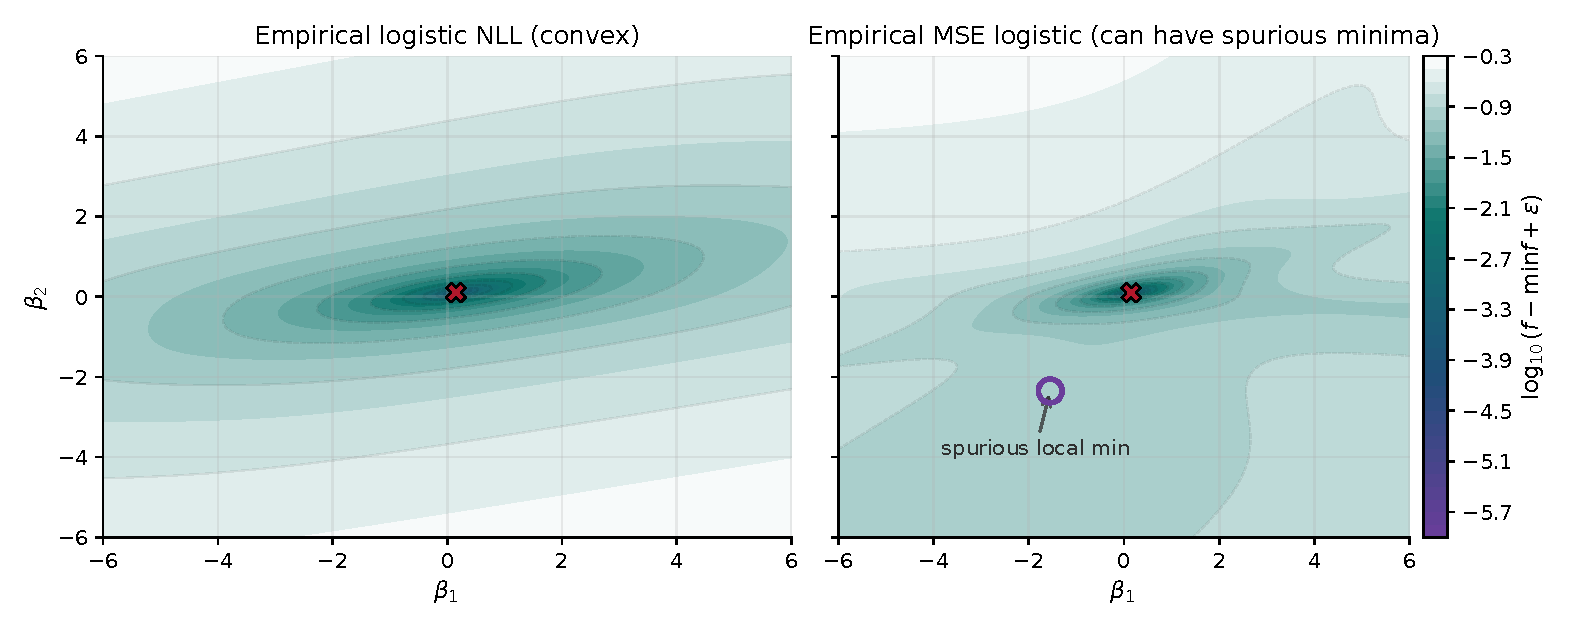
\includegraphics[width=\textwidth]{figures/handouts/convexity_optimization/fig_logistic_empirical_spurious}
  \caption{Empirical logistic landscapes on the dataset in \Cref{ex:logistic-empirical-spurious}.
  The plots show $\log_{10}(f-\min f+\varepsilon)$ for each objective.
  The red X marks the global minimizer in each panel.
  Left: the NLL is convex (one basin).
  Right: the squared-loss objective can have a spurious local minimum (circled), so a local method can get stuck.}
  \label{fig:logistic-empirical-spurious}
\end{figure}

\begin{figure}[t]
  \centering
  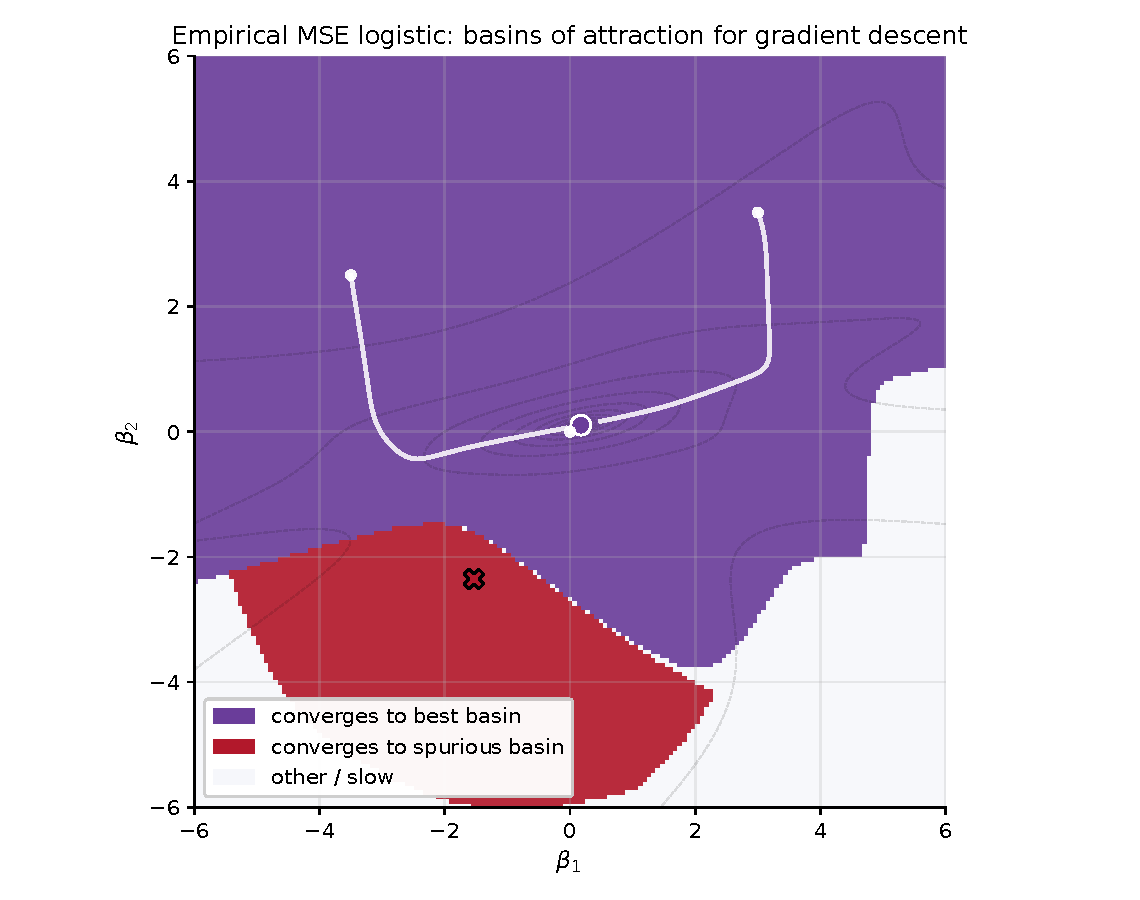
\includegraphics[width=0.92\textwidth]{figures/handouts/convexity_optimization/fig_logistic_empirical_basins}
  \caption{Basins of attraction for gradient descent on the empirical MSE-logistic objective in \Cref{ex:logistic-empirical-spurious}.
  The purple dot and red X mark the two local minimizers.
  Each initialization is colored by which local minimizer fixed-step GD (with $\eta=0.6$) converges to, and the overlaid paths show a few representative trajectories.}
  \label{fig:logistic-empirical-basins}
\end{figure}

Now assume a realizable population model:
\[
Y\mid X=x \sim \mathrm{Bernoulli}(p^\star(x)),
\qquad
p^\star(x) = \sigma(x^\top\beta^\star).
\]
Then the expected squared loss decomposes as
\[
\E\big[(Y-\sigma(X^\top\beta))^2\mid X\big]
= p^\star(X)(1-p^\star(X)) + \big(p^\star(X)-\sigma(X^\top\beta)\big)^2,
\]
so (up to an additive constant) the population objective becomes
\begin{equation}
R(\beta) = \E\big[(\sigma(X^\top\beta)-\sigma(X^\top\beta^\star))^2\big].
\label{eq:logistic-pop-risk}
\end{equation}

\begin{proposition}[One-point monotonicity in the realizable population squared-loss risk]
\label{prop:logistic-pop-one-point}
Assume $\E[\norm{X}_2]<\infty$, and let $R$ be as in \eqref{eq:logistic-pop-risk}. Then for all $\beta$,
\begin{equation}
\ip{\nabla R(\beta)}{\beta-\beta^\star} \ge 0.
\label{eq:one-point}
\end{equation}
In particular, along any ray $\beta(t)=\beta^\star+t(\beta-\beta^\star)$, the function $t\mapsto R(\beta(t))$ is nondecreasing for $t\ge 0$.
\end{proposition}

The next exercise isolates the population monotonicity calculation; structurally it plays the same role as the first-order convexity arguments in the Optimization unit.
\begin{exercise}[One-point monotonicity for realizable MSE-logistic]
\label{ex:logistic-one-point}
Prove \Cref{prop:logistic-pop-one-point}.
Let $\eta=X^\top\beta$ and $\eta^\star=X^\top\beta^\star$.
\begin{enumerate}[leftmargin=*]
  \item Differentiate under the expectation in \eqref{eq:logistic-pop-risk} to show that
  \[
  \nabla R(\beta)
  =2\,\E\Big[(\sigma(\eta)-\sigma(\eta^\star))\,\sigma'(\eta)\,X\Big].
  \]
  \item Show that
  \[
  \ip{\nabla R(\beta)}{\beta-\beta^\star}
  =2\,\E\Big[\sigma'(\eta)\,(\sigma(\eta)-\sigma(\eta^\star))(\eta-\eta^\star)\Big],
  \]
  and conclude it is nonnegative using only that $\sigma$ is increasing and $\sigma'\ge 0$.
  \item Deduce the ray-monotonicity statement by differentiating $g(t)=R(\beta^\star+t(\beta-\beta^\star))$.
\end{enumerate}
\end{exercise}

\SolutionBox[14]{%
\emph{Part (1).}
Differentiate \eqref{eq:logistic-pop-risk} under the expectation:
\[
R(\beta)=\E\big[(\sigma(X^\top\beta)-\sigma(X^\top\beta^\star))^2\big].
\]
Using the chain rule, $\nabla_\beta\sigma(X^\top\beta)=\sigma'(X^\top\beta)\,X$, hence
\[
\nabla R(\beta)
=2\,\E\Big[(\sigma(\eta)-\sigma(\eta^\star))\,\sigma'(\eta)\,X\Big],
\qquad
\eta=X^\top\beta,\ \eta^\star=X^\top\beta^\star.
\]

\emph{Part (2).}
Take the inner product with $(\beta-\beta^\star)$ and use $\ip{X}{\beta-\beta^\star}=\eta-\eta^\star$:
\[
\ip{\nabla R(\beta)}{\beta-\beta^\star}
=2\,\E\Big[\sigma'(\eta)\,(\sigma(\eta)-\sigma(\eta^\star))(\eta-\eta^\star)\Big].
\]
Since $\sigma'(\eta)\ge 0$ and $\sigma$ is increasing, we have
$(\sigma(\eta)-\sigma(\eta^\star))(\eta-\eta^\star)\ge 0$ pointwise.
Therefore the integrand is pointwise nonnegative, and the expectation is nonnegative as claimed.

\emph{Part (3) (ray monotonicity).}
For the ray $\beta(t)=\beta^\star+t(\beta-\beta^\star)$, define $g(t)=R(\beta(t))$.
By the chain rule,
\[
g'(t)=\ip{\nabla R(\beta(t))}{\beta-\beta^\star}\ge 0,
\]
so $t\mapsto R(\beta(t))$ is nondecreasing for $t\ge 0$.
(The argument uses only that the link is increasing with nonnegative derivative, so it holds for any such link function.)%
}

\begin{corollary}[Realizable population MSE-logistic has no spurious local minima]
\label{cor:logistic-pop-no-spurious}
Under the assumptions of \Cref{prop:logistic-pop-one-point}, every local minimizer of the realizable population risk $R$ in \eqref{eq:logistic-pop-risk} is global.
If in addition $\E[XX^\top]\succ 0$, then the unique global minimizer is $\beta^\star$.
\end{corollary}

\begin{exercise}[Stationarity + one-point monotonicity $\Rightarrow$ no spurious local minima]
\label{ex:logistic-one-point-no-spurious}
Prove \Cref{cor:logistic-pop-no-spurious} from \Cref{prop:logistic-pop-one-point}.
\begin{enumerate}[leftmargin=*]
  \item Let $\bar\beta$ be a local minimizer. Since $R$ is differentiable, $\nabla R(\bar\beta)=0$.
  Combine this with \Cref{eq:one-point} to show that
  \[
    0
    = \ip{\nabla R(\bar\beta)}{\bar\beta-\beta^\star}
    = 2\,\E\Big[\sigma'(\bar\eta)\,(\sigma(\bar\eta)-\sigma(\eta^\star))(\bar\eta-\eta^\star)\Big],
  \]
  where $\bar\eta=X^\top\bar\beta$ and $\eta^\star=X^\top\beta^\star$.
  Conclude that $\sigma(X^\top\bar\beta)=\sigma(X^\top\beta^\star)$ almost surely.
  \item Deduce that $R(\bar\beta)=0$, so $\bar\beta$ is a global minimizer.
  \item For uniqueness: show that if $R(\beta)=0$, then $X^\top(\beta-\beta^\star)=0$ almost surely, and deduce $\beta=\beta^\star$ under $\E[XX^\top]\succ 0$.
\end{enumerate}
\end{exercise}

\SolutionBox[14]{%
\emph{Part (1).}
Let $\bar\beta$ be a local minimizer of the differentiable function $R$.
Then $\nabla R(\bar\beta)=0$.
Applying \Cref{prop:logistic-pop-one-point} at $\beta=\bar\beta$ gives
\[
0
= \ip{\nabla R(\bar\beta)}{\bar\beta-\beta^\star}
= 2\,\E\Big[\sigma'(\bar\eta)\,(\sigma(\bar\eta)-\sigma(\eta^\star))(\bar\eta-\eta^\star)\Big],
\qquad \bar\eta=X^\top\bar\beta,\ \eta^\star=X^\top\beta^\star.
\]
The integrand is pointwise nonnegative because $\sigma'(\bar\eta)\ge 0$ and $\sigma$ is increasing, so the expectation can vanish only if the integrand is zero almost surely.
Since $\sigma'(z)>0$ for every finite $z$, this implies
\[
(\sigma(\bar\eta)-\sigma(\eta^\star))(\bar\eta-\eta^\star)=0
\qquad\text{almost surely.}
\]
Because $\sigma$ is strictly increasing, the product above is zero if and only if $\bar\eta=\eta^\star$, equivalently $\sigma(X^\top\bar\beta)=\sigma(X^\top\beta^\star)$ almost surely.

\emph{Part (2).}
If $\sigma(X^\top\bar\beta)=\sigma(X^\top\beta^\star)$ almost surely, then the integrand in \eqref{eq:logistic-pop-risk} vanishes almost surely, so
\[
R(\bar\beta)=\E\big[(\sigma(X^\top\bar\beta)-\sigma(X^\top\beta^\star))^2\big]=0.
\]
Since $R(\beta^\star)=0$ as well, $\bar\beta$ is a global minimizer.

\emph{Part (3) (uniqueness).}
If $R(\beta)=0$, then
\[
\E\big[(\sigma(X^\top\beta)-\sigma(X^\top\beta^\star))^2\big]=0,
\]
so $\sigma(X^\top\beta)=\sigma(X^\top\beta^\star)$ almost surely.
Since $\sigma$ is strictly increasing, this implies $X^\top(\beta-\beta^\star)=0$ almost surely.
Taking expectations yields
$(\beta-\beta^\star)^\top\E[XX^\top](\beta-\beta^\star)=0$.
If $\E[XX^\top]\succ 0$, then the quadratic form is strictly positive unless $\beta=\beta^\star$, so $\beta^\star$ is the unique global minimizer.%
}

The population MSE-logistic risk is nonconvex, but it still has the simple geometry that moving away from $\beta^\star$ does not help along any ray from $\beta^\star$.
This is qualitatively different from objectives like ecological logistic regression (\Cref{sec:ecological-logistic}), where aggregation introduces intrinsic nonconvexity and the landscape can have many distinct basins even under a clean population model.

Even with this benign global geometry, gradient descent can be slow because of saturation and flat plateaus.
The one-point monotonicity in \Cref{prop:logistic-pop-one-point} is a global geometry guarantee, but it is not a rate guarantee.
Far from $\beta^\star$, the squared-loss logistic objective can become very flat because the logistic link saturates:
$\sigma(z)\to 0$ or $1$ and $\sigma'(z)\to 0$ as $|z|\to\infty$.
The squared-loss gradient carries a factor of $\sigma'(X^\top\beta)$, so when the model is very confident (large $|X^\top\beta|$), the gradient can be tiny even if the objective value is not close to its minimum.
This mirrors the ``confidence weights'' story for convex NLL objectives:
in logistic NLL, curvature is largest near the decision boundary, while very confident points contribute little.
For squared loss, that same saturation suppresses the \emph{descent signal} itself, producing plateaus where $\norm{\nabla R(\beta)}_2$ is small even though $R(\beta)-R(\beta^\star)$ is not.

\begin{proposition}[Realizable squared-loss logistic: arbitrarily flat far from $\beta^\star$]
\label{prop:logistic-pop-flat}
Assume $\E[\norm{X}_2]<\infty$ and let $R$ be the realizable population risk \eqref{eq:logistic-pop-risk}.
Define $g(t)=R(t\beta^\star)$ for $t\ge 1$.
Then:
\begin{enumerate}[leftmargin=*]
  \item $g$ is nondecreasing on $[1,\infty)$ and converges to a finite limit $g(\infty)$.
  \item $\lim_{t\to\infty} g'(t)=0$ and $\lim_{t\to\infty}\norm{\nabla R(t\beta^\star)}_2=0$.
  \item If $\Pr(X^\top\beta^\star\neq 0)>0$, then $g(\infty)>0$.
\end{enumerate}
In particular, there are directions along which the landscape becomes arbitrarily flat even though the excess risk stays bounded away from $0$.
\end{proposition}

\emph{Proof idea.} See Exercise~\ref{ex:logistic-plateau}.

\begin{exercise}[Prove the plateau]
\label{ex:logistic-plateau}
In the realizable population model, let $g(t)=R(t\beta^\star)$ for $t\ge 1$.
\begin{enumerate}[leftmargin=*]
  \item Show that
  \[
    g'(t)=2\,\E\big[(\sigma(t\eta^\star)-\sigma(\eta^\star))\,\sigma'(t\eta^\star)\,\eta^\star\big],
    \qquad \eta^\star=X^\top\beta^\star,
  \]
  and conclude that $g$ is nondecreasing (hence $g(t)\to g(\infty)$ since $0\le g(t)\le 1$).
  \item Show that $g'(t)\to 0$ and $\nabla R(t\beta^\star)\to 0$ as $t\to\infty$.
  Interpret this as: \emph{without} a PL/strong-convexity-type condition, small gradient does not imply near-optimality.
  \item Assume $\Pr(\eta^\star\neq 0)>0$.
  Show that $g(\infty)>0$.
\end{enumerate}
\end{exercise}

\SolutionBox[12]{%
Write $\eta^\star=X^\top\beta^\star$ so that $g(t)=\E[(\sigma(t\eta^\star)-\sigma(\eta^\star))^2]$.

\emph{Part (1).}
Differentiate under the expectation:
by the chain rule,
\[
\frac{d}{dt}\sigma(t\eta^\star)=\sigma'(t\eta^\star)\,\eta^\star,
\]
so
\[
g'(t)
=\E\Big[2(\sigma(t\eta^\star)-\sigma(\eta^\star))\cdot \sigma'(t\eta^\star)\,\eta^\star\Big]
=2\,\E\big[(\sigma(t\eta^\star)-\sigma(\eta^\star))\,\sigma'(t\eta^\star)\,\eta^\star\big].
\]
For $t\ge 1$, $\sigma(t\eta^\star)-\sigma(\eta^\star)$ has the same sign as $(t-1)\eta^\star$ since $\sigma$ is increasing.
Because $\sigma'\ge 0$, the integrand is pointwise nonnegative, hence $g'(t)\ge 0$ and $g$ is nondecreasing.
Since $g(t)\in[0,1]$, it follows that $g(t)\to g(\infty)$ for some finite limit $g(\infty)$.

\emph{Part (2).}
For each fixed $\eta^\star\neq 0$, we have $t\eta^\star\to \pm\infty$ and therefore $\sigma'(t\eta^\star)\to 0$ as $t\to\infty$.
Also,
\[
\big|(\sigma(t\eta^\star)-\sigma(\eta^\star))\,\sigma'(t\eta^\star)\,\eta^\star\big|
\le \sigma'(0)\,|\eta^\star|
\le \sigma'(0)\,\norm{\beta^\star}_2\,\norm{X}_2,
\]
which is integrable since $\E[\norm{X}_2]<\infty$.
We will use the following standard fact: if random variables $Z_t$ satisfy $|Z_t|\le W$ with $\E[W]<\infty$ and $Z_t\to 0$ almost surely, then $\E[Z_t]\to 0$.
Applying this fact here gives $g'(t)\to 0$ as $t\to\infty$.

\smallskip
Similarly, differentiating \eqref{eq:logistic-pop-risk} gives
\[
\nabla R(t\beta^\star)
=2\,\E\big[(\sigma(t\eta^\star)-\sigma(\eta^\star))\,\sigma'(t\eta^\star)\,X\big].
\]
The integrand norm is bounded by $2\sigma'(0)\norm{X}_2$, and for each fixed $X$ the factor $\sigma'(t\eta^\star)$ tends to $0$ (or the bracketed term vanishes when $\eta^\star=0$), so the same reasoning lets us pass the limit through the expectation and conclude $\nabla R(t\beta^\star)\to 0$.

\emph{Part (3).}
As $t\to\infty$ we have $\sigma(t\eta^\star)\to 1$ when $\eta^\star>0$, $\sigma(t\eta^\star)\to 0$ when $\eta^\star<0$, and $\sigma(t\eta^\star)=\sigma(\eta^\star)=1/2$ when $\eta^\star=0$.
Since $0\le (\sigma(t\eta^\star)-\sigma(\eta^\star))^2\le 1$, we can apply the same fact (with $W=1$) to pass the limit through the expectation and obtain
\[
g(\infty)=\E\Big[(1-\sigma(\eta^\star))^2\mathbf{1}\{\eta^\star>0\} + \sigma(\eta^\star)^2\mathbf{1}\{\eta^\star<0\}\Big].
\]
If $\Pr(\eta^\star\neq 0)>0$, then the integrand is strictly positive on $\{\eta^\star\neq 0\}$, so $g(\infty)>0$.

Along this ray, the risk can remain bounded away from $0$ while the gradient (and directional derivative) goes to $0$.
Without a condition like PL/strong convexity, a small gradient does not by itself certify near-optimality.
}

Conditions like strong convexity or the PL inequality (\Cref{def:pl-inequality}) prevent this phenomenon: they rule out large flat regions away from the optimum by relating gradient size to suboptimality.
\Cref{prop:logistic-pop-flat} shows the realizable squared-loss logistic risk does not have such a global guarantee in general.

In the realizable population model, the one-point monotonicity in \Cref{prop:logistic-pop-one-point} is a \emph{global} geometric statement.
To get an actual rate for gradient descent, we also need a \emph{local curvature} condition near $\beta^\star$.
One simple sufficient condition is bounded features, which implies local strong convexity (hence a linear rate) around the optimum.

\begin{proposition}[Local linear convergence of gradient descent near $\beta^\star$]
\label{prop:logistic-pop-local-rate}
Assume $\E[XX^\top]\succeq \lambda I_d$ and $\norm{X}_2\le R$ almost surely for some $\lambda,R>0$.
Then at $\beta^\star$,
\[
\Hess R(\beta^\star)\succeq m_0 I_d,
\qquad
m_0 = 2\,\sigma'(R\norm{\beta^\star}_2)^2\,\lambda,
\]
and there exist $r>0$ and constants $0<m\le L<\infty$ such that the population risk $R$ in \eqref{eq:logistic-pop-risk} is $m$-strongly convex and $L$-smooth on the ball $\{\beta:\ \norm{\beta-\beta^\star}_2\le r\}$.
Consequently, gradient descent with step size $1/L$ initialized in this ball satisfies
\[
R(\beta^{(k)})-R(\beta^\star)
\le \left(1-\frac{m}{L}\right)^k\bigl(R(\beta^{(0)})-R(\beta^\star)\bigr)
\qquad\text{(see \citealp[\S9.3]{boyd_vandenberghe_2004_convex}).}
\]
\end{proposition}

\begin{proof}
Differentiate \eqref{eq:logistic-pop-risk} twice.
At $\beta=\beta^\star$, the cross term vanishes and the Hessian simplifies to
\[
\Hess R(\beta^\star)=2\,\E\big[\sigma'(X^\top\beta^\star)^2\,XX^\top\big].
\]
Since $\norm{X^\top\beta^\star}\le \norm{X}_2\norm{\beta^\star}_2\le R\norm{\beta^\star}_2$ almost surely, we have
$\sigma'(X^\top\beta^\star)\ge \sigma'(R\norm{\beta^\star}_2)>0$ almost surely (since $\sigma'$ is even and decreases with $|z|$), hence
\[
\Hess R(\beta^\star)\succeq 2\,\sigma'(R\norm{\beta^\star}_2)^2\,\E[XX^\top]\succeq 2\,\sigma'(R\norm{\beta^\star}_2)^2\,\lambda I_d.
\]
This is the claimed bound with $m_0=2\,\sigma'(R\norm{\beta^\star}_2)^2\,\lambda$.
Because $R$ is twice continuously differentiable and $\norm{X}_2\le R$ almost surely, $\Hess R(\beta)$ varies continuously in $\beta$ and is bounded on compact sets.
Therefore, on a sufficiently small ball around $\beta^\star$, the Hessian is bounded below by (say) $\tfrac12 m_0 I_d$ and above by $L I_d$ for some finite $L$, which gives local strong convexity and smoothness.
The linear convergence rate for gradient descent on an $m$-strongly convex and $L$-smooth function is standard (cited above).
\end{proof}

Under misspecification, hard multimodality can return.
If $p^\star(x)$ is not representable as $\sigma(x^\top\beta)$ (e.g.\ marginalizing over latent classes can yield mixtures of logits), then \eqref{eq:one-point} need not hold, and the population squared-loss risk can become bimodal with spurious local minima.
Benign global geometry often hinges on model and data assumptions.
This is one reason MLE (convex NLL) is often more stable than squared-loss fitting in logistic-type binary regression models.

\begin{example}[Misspecification can create a spurious local minimum for squared-loss logistic regression]
\label{ex:logistic-misspecified-spurious}
Consider a 1D feature $X$ that takes values $\{-2,-1,1,2\}$ with equal probability, and parameterize $\beta=(\beta_0,\beta_1)$ so that $q_\beta(x)=\sigma(\beta_0+\beta_1 x)$.
Let the true conditional probabilities be
\[
p^\star(-2)=0.49,\quad p^\star(-1)=0.87,\quad p^\star(1)=0.92,\quad p^\star(2)=0.36.
\]
This $p^\star$ is not representable as $q_\beta$, since it is not monotone in $x$.

For the population squared-loss risk $R_{\mathrm{MSE}}(\beta)=\E[(q_\beta(X)-p^\star(X))^2]$, a direct evaluation shows two distinct basins:
numerically, evaluating $R_{\mathrm{MSE}}$ on a grid reveals a global minimizer and a spurious local minimizer.
See \Cref{fig:logistic-landscape-2d}.
\end{example}

\begin{figure}[t]
  \centering
  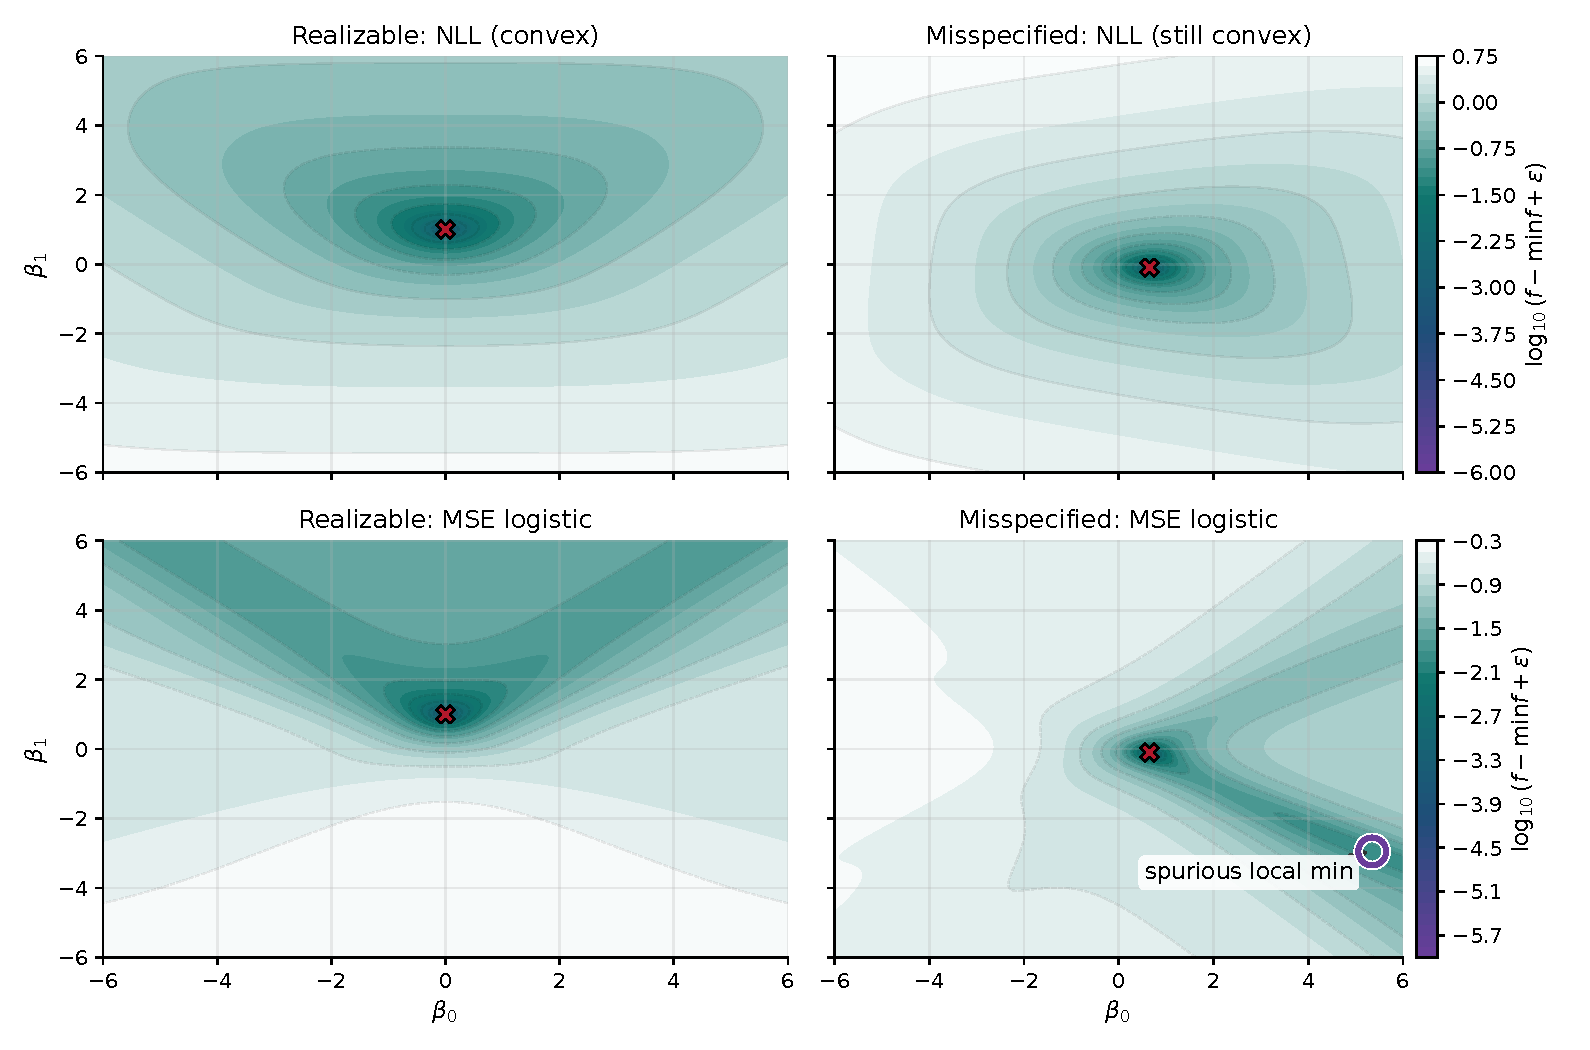
\includegraphics[width=\textwidth]{figures/handouts/convexity_optimization/fig_logistic_landscape_2d}
  \caption{A consistent contourf view of logistic landscapes in a 2D parameterization $\beta=(\beta_0,\beta_1)$.
  The plots show $\log_{10}(f-\min f+\varepsilon)$ for each objective, which makes basins comparable across panels.
  The red X marker indicates the global minimizer in each panel; in the bottom-right plot, the circled point is a spurious local minimum.
  In this example, the NLL landscape is unimodal in both realizable and misspecified settings, while the squared-loss landscape can develop extra basins under misspecification.}
  \label{fig:logistic-landscape-2d}
\end{figure}

% ------------------------------------------------------------
Example~I separates three distinct regimes.
Empirical MSE-logistic can create spurious basins; the realizable population risk has no spurious local minima but can still be slow because of broad plateaus; and misspecification can bring back genuinely wrong stable basins.
The response depends on the regime: use a stable objective when possible, use damping or line search when curvature is unreliable, and use restarts or stronger initializations when multiple basins are present.

% ------------------------------------------------------------
\section[Example II (phase retrieval)]{Example II: multimodality from symmetry, but only global optima in phase retrieval}
\label{sec:phase-retrieval}

In coherent diffraction imaging, optics, and astronomy, sensors measure intensities and lose phase.
A canonical real model is \emph{phase retrieval}:
\[
y_i = (a_i^\top x^\star)^2,\qquad i=1,\dots,m,
\]
where $x^\star\in\R^d$ is the unknown signal and $a_i$ are known sensing vectors.
A standard nonconvex least-squares objective is
\begin{equation}
F(x)=\frac{1}{4m}\sum_{i=1}^m\big((a_i^\top x)^2 - y_i\big)^2.
\label{eq:phase-empirical}
\end{equation}
This objective is nonconvex for structural reasons (it involves squares of linear forms),
and it is \emph{inherently} multimodal because $x^\star$ and $-x^\star$ generate the same data.

Like squared-loss logistic regression, phase retrieval is a smooth, nonconvex least-squares objective.
But here the nonconvexity is driven primarily by a \emph{symmetry}: $x^\star$ and $-x^\star$ generate the same data.
In population (for Gaussian designs), this symmetry produces multiple global optima but \emph{no} suboptimal local minima; the remaining stationary points are saddles.
This is ``benign'' nonconvexity (a strict-saddle picture), and it contrasts with ecological logistic regression (\Cref{sec:ecological-logistic}), where aggregation creates intrinsic nonconvexity and can lead to many distinct basins.
This ``benign geometry'' picture (multiple equivalent global minimizers; strict saddles elsewhere) appears broadly in modern tractable nonconvex problems; see \citet[\S2]{sun_qu_wright_2015_nonconvex_not_scary} and \citet[\S1]{zhang_qu_wright_2020_symmetry_geometry}.

\begin{figure}[t]
  \centering
  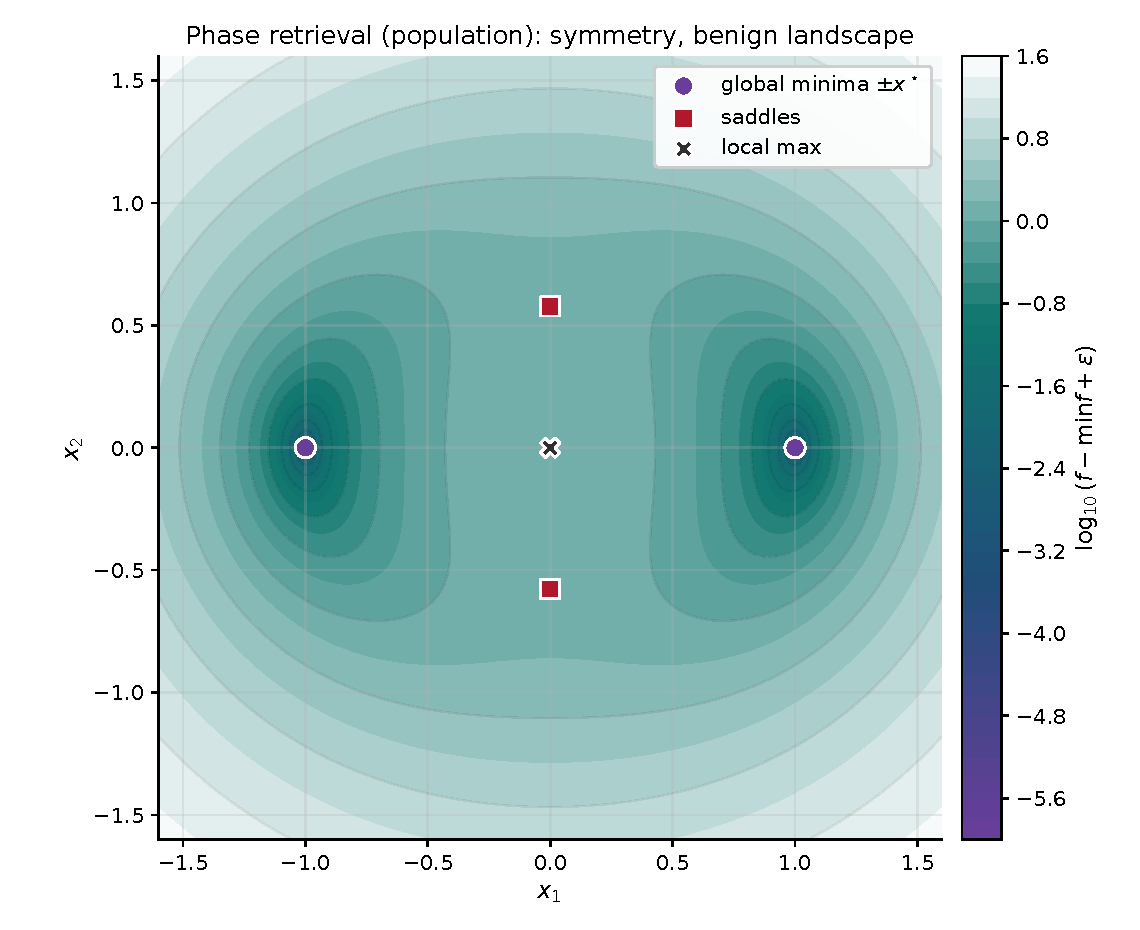
\includegraphics[width=0.86\textwidth]{figures/handouts/convexity_optimization/fig_phase_retrieval_landscape}
  \caption{Population phase retrieval in $d=2$: the landscape is nonconvex and symmetric ($x\sim -x$), but the only local minima are the two global minima $\pm x^\star$; other critical points are saddles or a local maximum at the origin.}
  \label{fig:phase-retrieval-landscape}
\end{figure}

For a clean population model, assume $a\sim N(0,I_d)$ and consider the \emph{population} objective
\begin{equation}
  f(x)=\frac12\,\E\Big[\big((a^\top x)^2 - (a^\top x^\star)^2\big)^2\Big].
  \label{eq:phase-pop}
\end{equation}

\begin{proposition}[Population phase retrieval: nonconvex but no spurious local minima]
\label{prop:phase-retrieval-benign}
For $f$ in \eqref{eq:phase-pop},
\begin{equation}
  f(x)
  =\frac{3}{2}\norm{x}^4 - \norm{x}^2\norm{x^\star}^2 - 2\ip{x}{x^\star}^2 + \frac{3}{2}\norm{x^\star}^4,
  \label{eq:phase-pop-closed-form}
\end{equation}
and the stationary points are:
\begin{enumerate}[leftmargin=*]
  \item global minima $x=\pm x^\star$ (value $0$),
  \item a local maximum at $x=0$,
  \item a saddle set $\{x:\ x\perp x^\star,\ \norm{x}=\norm{x^\star}/\sqrt{3}\}$.
\end{enumerate}
In particular, every local minimum is global.
\end{proposition}

\begin{exercise}[Phase retrieval: derive and classify the population stationary points]
\label{ex:phase-pop-derivation}
Prove \Cref{prop:phase-retrieval-benign}.
\begin{enumerate}[leftmargin=*]
  \item Expand \eqref{eq:phase-pop} and use the Gaussian fourth-moment identities
  \[
  \E[(a^\top u)^4]=3\norm{u}^4,
  \qquad
  \E[(a^\top u)^2(a^\top v)^2]=\norm{u}^2\norm{v}^2 + 2\ip{u}{v}^2,
  \]
  to obtain \eqref{eq:phase-pop-closed-form}.
  \item Differentiate \eqref{eq:phase-pop-closed-form} to get an explicit formula for $\nabla f(x)$.
  \item Solve $\nabla f(x)=0$ by decomposing $x=\alpha x^\star + u$ with $u\perp x^\star$.
  \item Classify the stationary points as global minima, a local maximum, and a saddle set.
\end{enumerate}
\end{exercise}

\SolutionBox[22]{%
\emph{Part (1) (closed form).}
Expanding the square in \eqref{eq:phase-pop} gives
\[
f(x)
=\frac12\,\E\big[(a^\top x)^4\big]
\;-\;\E\big[(a^\top x)^2(a^\top x^\star)^2\big]
\;+\;\frac12\,\E\big[(a^\top x^\star)^4\big].
\]
Apply the stated Gaussian fourth-moment identities with $u=x$ and $v=x^\star$ to get
\[
\E[(a^\top x)^4]=3\norm{x}^4,\qquad
\E[(a^\top x^\star)^4]=3\norm{x^\star}^4,
\]
and
\[
\E[(a^\top x)^2(a^\top x^\star)^2]=\norm{x}^2\norm{x^\star}^2 + 2\ip{x}{x^\star}^2.
\]
Substituting yields \eqref{eq:phase-pop-closed-form}.

\emph{Part (2) (gradient).}
Differentiate \eqref{eq:phase-pop-closed-form}:
\[
\nabla f(x)
= 6\norm{x}^2 x - 2\norm{x^\star}^2 x - 4\ip{x}{x^\star}x^\star
= (6\norm{x}^2-2\norm{x^\star}^2)x - 4\ip{x}{x^\star}x^\star.
\]

\emph{Part (3) (stationary points).}
Let $r=\norm{x^\star}_2$ and decompose $x=\alpha x^\star + u$ with $u\perp x^\star$.
Then $\ip{x}{x^\star}=\alpha r^2$ and $\norm{x}^2=\alpha^2r^2+\norm{u}^2$.
Setting $\nabla f(x)=0$ and matching the $u$ and $x^\star$ components gives
\[
(6\norm{x}^2-2r^2)\,u=0,
\qquad
\alpha\,(6\norm{x}^2-6r^2)=0.
\]
If $u=0$, then either $\alpha=0$ (so $x=0$) or $\norm{x}^2=r^2$ (so $\alpha=\pm 1$ and $x=\pm x^\star$).
If $u\neq 0$, then the first equation forces $\norm{x}^2=r^2/3$, and the second forces $\alpha=0$, hence
$x\perp x^\star$ and $\norm{x}=r/\sqrt{3}$.
This gives exactly the stationary-point list in \Cref{prop:phase-retrieval-benign}.

\emph{Part (4) (classification).}
Since $f$ in \eqref{eq:phase-pop} is an expectation of a square, $f(x)\ge 0$ for all $x$.
Also $f(\pm x^\star)=0$, so $\pm x^\star$ are global minima.

For $x=0$, the expansion \eqref{eq:phase-pop-closed-form} shows
\[
f(0)-f(x)= r^2\norm{x}^2 + 2\ip{x}{x^\star}^2 - \frac{3}{2}\norm{x}^4,
\]
which is strictly positive for all sufficiently small $x\neq 0$ (the quadratic term dominates), so $x=0$ is a local maximum.

Finally, if $x\perp x^\star$ and $\norm{x}=r/\sqrt{3}$, then the univariate restriction $t\mapsto f(x+t x^\star)$ has negative second derivative at $t=0$, so there is a direction of negative curvature.
Hence these points are saddles, and every local minimum is global.%
}

This is symmetry-driven nonconvexity with a strict-saddle geometry:
every non-optimal stationary point has a direction of negative curvature.

Phase retrieval is typically approached via the two-stage template in \Cref{alg:two-stage-template}:
use a cheap global initializer, then run a local method.
In the Gaussian model, there is a clean way to build a provably good direction estimate from a simple moment identity.
Assume the noiseless Gaussian design model $a_i \stackrel{\mathrm{iid}}{\sim} N(0,I_d)$ with measurements $y_i=(a_i^\top x^\star)^2$.
Define the \emph{spectral matrix}
\[
  Y = \frac{1}{m}\sum_{i=1}^m y_i a_i a_i^\top.
\]
Also define the radius estimate
\[
  \hat r^2 = \frac{1}{m}\sum_{i=1}^m y_i,
\]
which satisfies $\E[\hat r^2]=\norm{x^\star}_2^2$.
If $\hat u$ is a unit-norm top eigenvector of $Y$, then the standard spectral initializer is $x^{(0)}=\hat r\,\hat u$.

The next proposition explains why this initialization is reasonable.
It shows that (i) the population matrix $\E[Y]$ has a unique leading eigenvector in the $x^\star$ direction, and (ii) if the empirical $Y$ is close to $\E[Y]$ in operator norm then its leading eigenvector must be close to $\pm x^\star/\norm{x^\star}_2$.
(Here $\norm{M}_{\mathrm{op}}$ denotes the operator norm, i.e.\ the largest absolute eigenvalue for a symmetric matrix $M$.)

\begin{proposition}[Gaussian phase retrieval: why the spectral initializer points at $x^\star$]
\label{prop:phase-spectral-init}
Assume $x^\star\neq 0$, let $a\sim N(0,I_d)$, and set $y=(a^\top x^\star)^2$.
Write $r=\norm{x^\star}_2$ and $u^\star=x^\star/r$.
Define the population matrix
\[
  Y_{\mathrm{pop}} = \E\big[y\,a a^\top\big]
  = \E\big[(a^\top x^\star)^2 a a^\top\big].
\]
Then
\[
  Y_{\mathrm{pop}}=r^2 I_d + 2x^\star(x^\star)^\top,
\]
so the unique leading eigenvector of $Y_{\mathrm{pop}}$ is $u^\star$.
Moreover, if $Y$ is any symmetric matrix satisfying
\[
\norm{Y-Y_{\mathrm{pop}}}_{\mathrm{op}} \le \varepsilon\, r^2
\qquad\text{for some }\varepsilon\in(0,1),
\]
then for every unit-norm leading eigenvector $\hat u$ of $Y$ there exists a sign $s\in\{\pm 1\}$ such that
$\norm{\hat u-su^\star}_2\le \sqrt{2\varepsilon}$.
\end{proposition}

\begin{exercise}[Phase retrieval: why spectral initialization points at $x^\star$]
\label{ex:phase-spectral-spike}
Prove \Cref{prop:phase-spectral-init}.
Conclude that if the empirical matrix $Y$ is close to $Y_{\mathrm{pop}}$ in operator norm, then its top eigenvector is close to $\pm u^\star$ and the spectral initializer $x^{(0)}=\hat r\,\hat u$ is close to $\pm x^\star$.
\emph{Hint:} to compute $Y_{\mathrm{pop}}$, you can either compute entries using the Gaussian fourth-moment identity
$\E[a_i a_j a_k a_\ell]=\delta_{ij}\delta_{k\ell}+\delta_{ik}\delta_{j\ell}+\delta_{i\ell}\delta_{jk}$,
or compute the entries directly by expanding.
For the perturbation bound, compare quadratic forms $v^\top Y v$ and use $|v^\top (Y-Y_{\mathrm{pop}}) v|\le \norm{Y-Y_{\mathrm{pop}}}_{\mathrm{op}}$ for unit $v$.
Finally, explain in a sentence why one expects $\norm{Y-Y_{\mathrm{pop}}}_{\mathrm{op}}$ to be small when $m$ is large in the Gaussian model.
\end{exercise}

\SolutionBox[20]{%
Write $u=x^\star$ and expand $y=(a^\top u)^2=\sum_{k,\ell} u_k u_\ell a_k a_\ell$.
For each entry $(i,j)$,
\[
\E\!\big[y\,a_i a_j\big]
=\sum_{k,\ell} u_k u_\ell\,\E[a_i a_j a_k a_\ell]
=\sum_{k,\ell} u_k u_\ell\bigl(\delta_{ij}\delta_{k\ell}+\delta_{ik}\delta_{j\ell}+\delta_{i\ell}\delta_{jk}\bigr).
\]
The first term gives $\delta_{ij}\sum_k u_k^2=\delta_{ij}\norm{u}_2^2$.
The second and third terms each give $u_i u_j$.
Thus $\E[y\,a_i a_j]=\norm{u}_2^2\,\delta_{ij}+2u_i u_j$, i.e.
$Y_{\mathrm{pop}}=\norm{u}_2^2 I_d + 2uu^\top$.

For eigenvalues, note that $Y_{\mathrm{pop}}u=(\norm{u}_2^2+2\norm{u}_2^2)u=3\norm{u}_2^2 u$.
If $w\perp u$, then $uu^\top w=0$ so $Y_{\mathrm{pop}}w=\norm{u}_2^2 w$.
Hence the unique top eigenspace is $\mathrm{span}\{u\}$.

Let $r=\norm{u}_2$ and $u^\star=u/r$.
Let $\hat u$ be a unit top eigenvector of $Y$.
Write $E=Y-Y_{\mathrm{pop}}$ and assume $\norm{E}_{\mathrm{op}}\le \varepsilon r^2$.
Then
\[
\hat u^\top Y_{\mathrm{pop}} \hat u
= \hat u^\top Y \hat u - \hat u^\top E \hat u
\ge \lambda_{\max}(Y) - \norm{E}_{\mathrm{op}}
\ge (u^\star)^\top Y u^\star - \norm{E}_{\mathrm{op}}
\ge 3r^2 - 2\varepsilon r^2.
\]
On the other hand,
$
\hat u^\top Y_{\mathrm{pop}} \hat u
= r^2 + 2r^2\,|\ip{\hat u}{u^\star}|^2.
$
Combining gives $|\ip{\hat u}{u^\star}|^2\ge 1-\varepsilon$.
Choosing the sign that maximizes the inner product,
\[
\min\{\norm{\hat u-u^\star}_2,\norm{\hat u+u^\star}_2\}^2
=2\bigl(1-|\ip{\hat u}{u^\star}|\bigr)
\le 2\bigl(1-|\ip{\hat u}{u^\star}|^2\bigr)
\le 2\varepsilon.
\]

The matrix $Y$ is an empirical average of i.i.d.\ symmetric matrices with mean $Y_{\mathrm{pop}}$.
To make this quantitative in high dimensions, one uses concentration inequalities for random matrices to bound $\norm{Y-Y_{\mathrm{pop}}}_{\mathrm{op}}$ with high probability; see \citet[\S2.2]{zhang_qu_wright_2020_symmetry_geometry} for discussion and references.
These probability tools are largely orthogonal to our focus here.%
}

Once you have an initialization that is close to $\pm x^\star$, the local stage behaves like the convex story again.
In the Gaussian population objective, $\pm x^\star$ are not only global minima: they are \emph{locally strongly convex} minima, so the standard local strong-convexity analysis from the Optimization unit gives a linear rate while the iterates remain in that neighborhood.

\begin{exercise}[Phase retrieval: local convexity near $\pm x^\star$ in the population objective]
\label{ex:phase-pop-local-strong-convex}
For the population objective $f$ in \eqref{eq:phase-pop-closed-form}, compute the Hessian $\Hess f(x)$ and show that
\[
\Hess f(x^\star)=4\norm{x^\star}_2^2 I_d + 8x^\star(x^\star)^\top.
\]
Deduce the eigenvalues of $\Hess f(x^\star)$ and interpret this as a local condition-number statement near $x^\star$.
\end{exercise}

\SolutionBox[12]{%
Differentiate the gradient formula in the solution to \Cref{ex:phase-pop-derivation}:
for $x\in\R^d$,
\[
\Hess f(x)=12xx^\top + (6\norm{x}_2^2-2\norm{x^\star}_2^2)I_d - 4x^\star(x^\star)^\top.
\]
At $x=x^\star$ this becomes
\[
\Hess f(x^\star)=(12-4)x^\star(x^\star)^\top + 4\norm{x^\star}_2^2 I_d
=8x^\star(x^\star)^\top + 4\norm{x^\star}_2^2 I_d.
\]
Along $u^\star=x^\star/\norm{x^\star}_2$ the eigenvalue is $12\norm{x^\star}_2^2$, and along any direction orthogonal to $x^\star$ the eigenvalue is $4\norm{x^\star}_2^2$.
So near $x^\star$ the population objective is well conditioned (local condition number $3$), which is exactly the regime where local methods behave like in the convex case.%
}

These pieces give the standard Gaussian-model story:
spectral initialization supplies a direction close to $\pm x^\star$, and the local geometry near $\pm x^\star$ is strongly convex, so local methods converge quickly once initialized there.
Rigorous finite-sample analyses follow this template; see \citet[\S2.2]{zhang_qu_wright_2020_symmetry_geometry} and references therein.

Phase retrieval shows a different kind of nonconvexity.
The sign symmetry creates multiple optima, but they are equivalent, and the remaining stationary points are saddles rather than bad local minima.
The right response is therefore not exhaustive global search; it is a coarse initializer, such as a spectral method, followed by local refinement inside the basin of $\pm x^\star$.



% ------------------------------------------------------------
\section[Example III (ecological logistic)]{Example III: hard nonconvexity from aggregation in ecological logistic regression}
\label{sec:ecological-logistic}

In some applications we observe covariates at the unit level but only aggregated outcomes.
For example, we might see covariates $x_{g,1},\dots,x_{g,n_g}$ for individuals in a group (a precinct, a cohort, a batch),
but instead of observing the binary outcomes $Y_{g,i}\in\{0,1\}$ we only observe the group total
\[
Z_g = \sum_{i=1}^{n_g} Y_{g,i}.
\]
Many different binary vectors $(Y_{g,1},\dots,Y_{g,n_g})$ can produce the same total $Z_g$, so the likelihood for $\beta$ must marginalize over a large discrete set of latent ``assignments.''

Assume a logistic model at the unit level:
\[
\Pr(Y_{g,i}=1\mid x_{g,i},\beta)=\sigma(x_{g,i}^\top\beta),
\qquad i=1,\dots,n_g,
\]
with conditional independence across $i$ given the covariates.
Write $p_{g,i}(\beta)=\sigma(x_{g,i}^\top\beta)$.
Then $Z_g$ is a sum of independent but non-identically distributed Bernoulli random variables (a Poisson--binomial model), and the marginal likelihood contains $\binom{n_g}{z_g}$ terms.
The resulting negative log-likelihood is typically nonconvex in $\beta$.
This combinatorial marginalization also creates a separate difficulty that is easy to miss if we focus only on the geometry:
when $n_g$ is large, the likelihood term $\Pr(Z_g=z_g\mid x_{g,1},\dots,x_{g,n_g},\beta)$ can be expensive to evaluate repeatedly inside an optimizer.
The naive computation is literally a sum over $\binom{n_g}{z_g}$ assignments (as in \Cref{ex:eco-logistic-nonconvex}), which is intractable for large groups.
This ``optimization + marginalization'' pattern is common in latent-variable models: hard landscapes and expensive objective evaluations can come together.

An empirical negative log-likelihood objective for $G$ independent groups is
\begin{equation}
  f(\beta)
  =
  -\frac{1}{G}\sum_{g=1}^G \log \Pr(Z_g=z_g \mid x_{g,1},\dots,x_{g,n_g},\beta).
  \label{eq:eco-logistic-obj}
\end{equation}
Two edge cases are instructive.
In the special case where the covariates are constant within each group ($x_{g,i}\equiv x_g$), we have
$Z_g\sim \mathrm{Binomial}(n_g,\sigma(x_g^\top\beta))$, and \eqref{eq:eco-logistic-obj} reduces to the usual convex binomial logistic-regression objective from the Optimization unit.
At the other extreme, if $d=1$ with $\beta=(\beta_0,\beta_1)$ and each group contains covariates in $\pm$ pairs (for every $x$ the value $-x$ appears with the same multiplicity), then the marginal likelihood is symmetric in the slope: it is unchanged under $\beta_1\mapsto -\beta_1$.
This kind of symmetry reflects a genuine non-identifiability from totals alone.

\begin{exercise}[Ecological logistic regression: two easy special cases]
\label{ex:eco-logistic-edge-cases}
\begin{enumerate}[leftmargin=*]
  \item Suppose $x_{g,i}\equiv x_g$ within each group.
  Show that $Z_g\sim \mathrm{Binomial}(n_g,\sigma(x_g^\top\beta))$ and conclude that the corresponding negative log-likelihood is convex in $\beta$.
  \item Assume $d=1$ with $\beta=(\beta_0,\beta_1)$ and suppose the multiset $\{x_1,\dots,x_n\}$ is symmetric: for every $x$ it contains $-x$ with the same multiplicity.
  Show that, for every $z$,
  \[
    \Pr(Z=z\mid x_1,\dots,x_n,(\beta_0,\beta_1))
    =
    \Pr(Z=z\mid x_1,\dots,x_n,(\beta_0,-\beta_1)).
  \]
  Conclude that the likelihood for $\beta_1$ is an even function, so the sign of the slope is not identifiable from $Z$ alone in such a balanced design.
\end{enumerate}
\end{exercise}

\SolutionBox[14]{%
\emph{Part (1).}
If $x_{g,i}\equiv x_g$, then conditional on $x_g$ the unit-level outcomes are i.i.d.\ Bernoulli with success probability $\sigma(x_g^\top\beta)$.
Therefore $Z_g=\sum_{i=1}^{n_g}Y_{g,i}\sim \mathrm{Binomial}(n_g,\sigma(x_g^\top\beta))$.
Up to an additive constant (independent of $\beta$), the per-group negative log-likelihood can be written as a function of the scalar $\eta=x_g^\top\beta$:
\[
\ell_g(\beta)
= -z_g\,\eta + n_g\log(1+e^\eta).
\]
Since $\frac{d^2}{d\eta^2}\ell_g(\eta)=n_g\,\sigma'(\eta)\ge 0$, the map $\eta\mapsto \ell_g(\eta)$ is convex.
Composing a convex function with a linear map $\beta\mapsto x_g^\top\beta$ preserves convexity, so $\ell_g$ is convex in $\beta$.
Summing over $g$ preserves convexity, hence the full objective is convex.

\emph{Part (2).}
Write $p_i(\beta_0,\beta_1)=\sigma(\beta_0+\beta_1 x_i)$.
Replacing $\beta_1$ by $-\beta_1$ replaces $p_i$ by $\tilde p_i=\sigma(\beta_0-\beta_1 x_i)$.
By the assumed symmetry of the multiset $\{x_i\}$, the multiset $\{\tilde p_i\}$ is the same as $\{p_i\}$ up to a permutation (each $x$ is paired with $-x$).
But the distribution of $Z=\sum_i Y_i$ depends only on the multiset of success probabilities, not on how they are ordered, so $\Pr(Z=z\mid x_1,\dots,x_n,(\beta_0,\beta_1))=\Pr(Z=z\mid x_1,\dots,x_n,(\beta_0,-\beta_1))$ for every $z$.
Thus the likelihood is an even function of $\beta_1$, which means the sign of the slope is not identifiable from totals in this balanced design.%
}

This example ties directly to the empirical-versus-population theme from Example~I.
There the bad basins can be a finite-sample artifact under benign population geometry; here the nonconvexity is intrinsic, because even under the correct model and infinite data aggregation forces us to marginalize over discrete latent assignments.
That marginalization step is also the bridge to the Expectation--maximization subsection of the Augmented-state optimization unit: once the assignments are latent, the natural algorithmic object is the EM update map, which alternates exact conditional expectations with parameter updates, rather than a single closed-form convex objective.

To emphasize this, it is useful to look at a \emph{population} version of \eqref{eq:eco-logistic-obj}.
Let $X=(x_1,\dots,x_n)$ denote a random group of covariates and let $Z$ be generated from the model under a true parameter $\beta^\star$.
Define the population objective
\[
F(\beta)=\E\big[-\log \Pr(Z\mid X,\beta)\big].
\]
Because the model is correctly specified, $F$ is minimized at (an observationally equivalent version of) $\beta^\star$.
However, as \Cref{fig:eco-logistic-pop-landscape} illustrates, $F$ can still have multiple separated basins and spurious local minima.

\begin{figure}[H]
  \centering
  \input{figures/handouts/convexity_optimization/fig_ecological_logistic_population_landscape}
  \caption{A toy \emph{population} objective for ecological logistic regression in a 2D parameterization $\beta=(\beta_0,\beta_1)$.
  Each group has $n=6$ units and is equally likely to have covariates $(-4,-3,-2,2,3,4)$, $(-3,-1,1,2,3,4)$, or $(-2,-1,1,2,3,4)$ (in $d=1$); outcomes are generated under $\beta^\star=(0.3,1.2)$.
  The plot shows $\log_{10}(F-\min F+\varepsilon)$, as in \Cref{fig:logistic-landscape-2d}; the red X marks $\beta^\star$ and the open circles mark three spurious local minima in this toy example.}
  \label{fig:eco-logistic-pop-landscape}
\end{figure}

\begin{exercise}[Ecological logistic regression: marginalization and nonconvexity]
\label{ex:eco-logistic-nonconvex}
Fix one group with covariates $x_1,\dots,x_n\in\R^d$ and observe $Z=z$.
Let $p_i(\beta)=\sigma(x_i^\top\beta)$.
\begin{enumerate}[leftmargin=*]
  \item Show that
  \[
    \Pr(Z=z\mid x_1,\dots,x_n,\beta)
    =
    \sum_{\substack{S\subseteq\{1,\dots,n\}\\|S|=z}}
    \ \prod_{i\in S} p_i(\beta)\prod_{j\notin S}\bigl(1-p_j(\beta)\bigr).
  \]
  Interpret this as summing over all ways to choose which $z$ units are the successes.
  \item Specialize to $n=2$ and $z=1$ in $d=1$ with covariates $x_1=a$ and $x_2=b$.
  Let $\ell(\beta)$ be the negative log-likelihood $-\log \Pr(Z=1\mid a,b,\beta)$ with no regularization.
  Show that $\ell''(0)=\tfrac12 ab$.
  Conclude that $\ell$ is not convex whenever $ab<0$.
\end{enumerate}
\end{exercise}

\SolutionBox[20]{%
\emph{Part (1).}
Condition on the covariates.
For any binary vector $y=(y_1,\dots,y_n)\in\{0,1\}^n$, conditional independence gives
\[
\Pr(Y_1=y_1,\dots,Y_n=y_n\mid x_1,\dots,x_n,\beta)
=
\prod_{i=1}^n p_i(\beta)^{y_i}\bigl(1-p_i(\beta)\bigr)^{1-y_i}.
\]
The event $\{Z=z\}$ is the union of all assignments $y$ with exactly $z$ ones, so summing over those assignments yields
\[
\Pr(Z=z\mid x_1,\dots,x_n,\beta)
=
\sum_{\substack{y\in\{0,1\}^n\\ \sum_i y_i=z}}
\ \prod_{i=1}^n p_i(\beta)^{y_i}\bigl(1-p_i(\beta)\bigr)^{1-y_i}.
\]
Reindexing the sum by the subset $S=\{i:\ y_i=1\}$ (which has $|S|=z$) gives the stated formula.

\emph{Part (2).}
For $n=2$ and $z=1$, let $p_1(\beta)=\sigma(a\beta)$ and $p_2(\beta)=\sigma(b\beta)$.
Then
\[
q(\beta)=\Pr(Z=1\mid a,b,\beta)
 = p_1(1-p_2) + (1-p_1)p_2
 = p_1+p_2-2p_1p_2,
\]
and $\ell(\beta)=-\log q(\beta)$.
At $\beta=0$ we have $p_1=p_2=\tfrac12$, so $q(0)=\tfrac12$.
Also $p_1'(\beta)=a\,p_1(1-p_1)$ and $p_2'(\beta)=b\,p_2(1-p_2)$, so $p_1'(0)=a/4$ and $p_2'(0)=b/4$.
A direct differentiation gives $q'(0)=0$ and
\[
q''(0)=-4p_1'(0)p_2'(0)=-4\cdot\frac{a}{4}\cdot\frac{b}{4}=-\frac{ab}{4}.
\]
Since $\ell'=-q'/q$ and $q'(0)=0$, we have $\ell''(0)=-(q''(0)/q(0))$ and therefore
\[
\ell''(0)
=-\frac{q''(0)}{q(0)}
=-\frac{-ab/4}{1/2}
=\frac{ab}{2}.
\]
If $ab<0$, then $\ell''(0)<0$, so $\ell$ is not convex.
}

Even though the landscape can be globally hard (and even the population objective can have spurious basins, as in \Cref{fig:eco-logistic-pop-landscape}), there is still a familiar ``convex'' story \emph{locally} around the true parameter under correct specification.
When the model is locally identifiable, the population objective has a neighborhood of $\beta^\star$ on which it is convex (indeed strongly convex).
One convenient way to see this in ecological logistic regression is to expose the probabilistic structure behind the gradient and Hessian: the observed-data objective involves marginalizing over latent assignments, and its Hessian can be written as a difference of two covariance matrices.
After averaging over the random total $Z$ under the true model, that difference becomes a covariance by the law of total covariance.

\begin{exercise}[Ecological logistic regression: DC structure and local convexity near $\beta^\star$]
\label{ex:eco-logistic-pop-local-convex}
Fix covariates $x_1,\dots,x_n\in\R^d$.
For $\beta\in\R^d$, let $V_1,\dots,V_n$ be independent Bernoulli random variables with
\[
\Pr(V_j=1\mid x_j,\beta)=\sigma(x_j^\top\beta),
\qquad j=1,\dots,n,
\]
and define
\[
U = \sum_{j=1}^n x_j V_j,
\qquad
Z = \sum_{j=1}^n V_j.
\]
For an observed total $Z=z$, write $L_z(\beta)=-\log \Pr(Z=z\mid x_1,\dots,x_n,\beta)$.
\begin{enumerate}[leftmargin=*]
  \item Show the \emph{difference-of-convex (DC)} form
  \[
  L_z(\beta)
  =\sum_{j=1}^n \log\bigl(1+e^{x_j^\top\beta}\bigr)
  -\log\left(\sum_{\substack{S\subseteq\{1,\dots,n\}\\|S|=z}} \exp\Big(\sum_{j\in S} x_j^\top\beta\Big)\right).
  \]
  \item Show that $\nabla L_z(\beta)=\E[U]-\E[U\mid Z=z]$.
  \item Show that $\Hess L_z(\beta)=\mathrm{Cov}(U)-\mathrm{Cov}(U\mid Z=z)$.
  (Hint: for $g(\beta)=\log\sum_k e^{a_k^\top\beta}$, the Hessian is the covariance of the vectors $\{a_k\}$ under the corresponding softmax weights.)
  \item Consider the population objective $F(\beta)=\E[L_Z(\beta)]$ when $Z$ is generated under a true parameter $\beta^\star$.
  Assuming the outer expectation defining $F$ can be differentiated twice under the integral sign, use the conditional law of total covariance,
  \[
    \mathrm{Cov}(U\mid X)=\E[\mathrm{Cov}(U\mid Z,X)\mid X] + \mathrm{Cov}(\E[U\mid Z,X]\mid X),
  \]
  to show that
  \[
    \E\big[\Hess L_Z(\beta^\star)\mid X\big]
    = \mathrm{Cov}\big(\E[U\mid Z,X]\mid X\big)\succeq 0.
  \]
  Deduce that
  \[
    \Hess F(\beta^\star)
    = \E\Big[\mathrm{Cov}\big(\E[U\mid Z,X]\mid X\big)\Big]\succeq 0.
  \]
  Conclude that if $\Hess F(\beta^\star)\succ 0$, then $F$ is locally strongly convex on a neighborhood of $\beta^\star$.
\end{enumerate}
\end{exercise}

\SolutionBox[22]{%
\emph{Part (1).}
Write $\eta_j=x_j^\top\beta$ and $p_j=\sigma(\eta_j)=e^{\eta_j}/(1+e^{\eta_j})$.
For any subset $S$ with $|S|=z$,
\[
\Pr(V_j=1\ \forall j\in S,\ V_j=0\ \forall j\notin S\mid x_1,\dots,x_n,\beta)
=\prod_{j\in S}p_j\prod_{j\notin S}(1-p_j)
=\frac{\exp(\sum_{j\in S}\eta_j)}{\prod_{j=1}^n(1+e^{\eta_j})}.
\]
Summing over all $S$ with $|S|=z$ gives
\[
\Pr(Z=z\mid x_1,\dots,x_n,\beta)
=\frac{\sum_{|S|=z}\exp(\sum_{j\in S}\eta_j)}{\prod_{j=1}^n(1+e^{\eta_j})}.
\]
Taking $-\log$ yields the stated DC representation.

\emph{Parts (2) and (3).}
The first term in $L_z$ has gradient $\sum_j \sigma(\eta_j)x_j$ and Hessian $\sum_j \sigma'(\eta_j)x_jx_j^\top$.
Since $U=\sum_j x_j V_j$ with independent Bernoulli coordinates, these are exactly $\E[U]$ and $\mathrm{Cov}(U)$.

For the second term, define a probability distribution on subsets $S$ of size $z$ by
\[
w_S(\beta)\propto \exp\Big(\sum_{j\in S}x_j^\top\beta\Big),
\qquad |S|=z.
\]
This is the conditional law of the success set $\{j:\ V_j=1\}$ given $Z=z$ under parameter $\beta$.
Therefore
\[
\nabla \log\Big(\sum_{|S|=z} e^{\sum_{j\in S}x_j^\top\beta}\Big)
  = \sum_{|S|=z} w_S(\beta)\sum_{j\in S}x_j
  = \E[U\mid Z=z],
\]
and differentiating once more gives
\[
\Hess\!\left(\log\Big(\sum_{|S|=z} e^{\sum_{j\in S}x_j^\top\beta}\Big)\right)
=\mathrm{Cov}(U\mid Z=z),
\]
which yields $\nabla L_z=\E[U]-\E[U\mid Z=z]$ and $\Hess L_z=\mathrm{Cov}(U)-\mathrm{Cov}(U\mid Z=z)$.

\emph{Part (4).}
Now let $X=(x_1,\dots,x_n)$ be random, and assume we may differentiate the outer expectation in $F(\beta)=\E[L_Z(\beta)]$ twice under the integral sign.
Conditional on $X$ and at $\beta^\star$, take expectations over $Z$:
\[
\E\big[\Hess L_Z(\beta^\star)\mid X\big]
=\mathrm{Cov}(U\mid X)-\E[\mathrm{Cov}(U\mid Z,X)\mid X].
\]
By the conditional law of total covariance,
\[
\mathrm{Cov}(U\mid X)
=\E[\mathrm{Cov}(U\mid Z,X)\mid X] + \mathrm{Cov}(\E[U\mid Z,X]\mid X),
\]
so the difference is
\[
\E\big[\Hess L_Z(\beta^\star)\mid X\big]
=\mathrm{Cov}(\E[U\mid Z,X]\mid X)\succeq 0.
\]
Taking outer expectations gives
\[
\Hess F(\beta^\star)
=\E\big[\Hess L_Z(\beta^\star)\big]
=\E\Big[\mathrm{Cov}(\E[U\mid Z,X]\mid X)\Big]\succeq 0.
\]
If this unconditional Hessian is positive definite, then by continuity of $\Hess F$ there exists a radius $r>0$ such that $\Hess F(\beta)\succeq \tfrac12 \Hess F(\beta^\star)\succ 0$ on $\{\beta:\ \norm{\beta-\beta^\star}_2\le r\}$, which implies local strong convexity of $F$ on that neighborhood.%
}

This example still fits the two-stage template in \Cref{alg:two-stage-template}, but the coarse stage is less structured.
In practice, one often uses multiple random starts or a warm start from a crude convex surrogate, then runs a local optimizer with line search or damping on the true nonconvex objective \eqref{eq:eco-logistic-obj} and keeps the best solution found.

Ecological logistic regression is the genuinely hard case in this note.
Aggregation forces a sum over latent assignments, so the objective can have many distinct basins even under correct specification.
The practical response is usually robust search rather than a single clever local method: several starts, warm starts from crude convex surrogates when available, and then local refinement with damping or line search on the true objective.



% ------------------------------------------------------------
\section{Diagnosing nonconvex objectives}
\label{sec:checklist-streamlined}

``Nonconvex'' is not a single regime.
Squared-loss logistic regression is close to convex: the empirical objective can have spurious minima, yet under realizability the population geometry is benign and locally strongly convex near $\beta^\star$.
Phase retrieval is symmetry-driven: there can be multiple equivalent optima but no bad local minima.
Ecological logistic regression is intrinsically hard because aggregation induces latent assignments and the resulting marginal likelihood can have many distinct basins.
The right response depends on which regime you are in: stable objectives when available, spectral or other coarse initialization when symmetry is the issue, and restarts or stronger surrogates when aggregation drives the hardness.
This is also the lens used in the Expectation--maximization subsection of the Augmented-state optimization unit: the basin picture remains central, but the relevant geometry is now the geometry of the EM operator and its population/sample perturbations.

A useful diagnosis is to ask whether the difficulty comes from finite-sample noise or the population model, from symmetry or non-identifiability, from genuinely suboptimal basins, from the lack of a global guarantee beyond convexity, or simply from poor local conditioning.
Carried back to the main notes, the point is not that nonconvexity is uniformly hopeless.
The real question is which part of the convex story breaks first: the basin structure, the conditioning inside a good basin, or only the finite-sample objective we happen to optimize.

\begin{table}[t]
  \centering
  \small
  \setlength{\tabcolsep}{4pt}
  \begin{tabular}{@{}p{0.18\textwidth}p{0.24\textwidth}p{0.26\textwidth}p{0.24\textwidth}@{}}
    \toprule
    Example & Source of nonconvexity & Global geometry & Typical response \\
    \midrule
    Logistic: NLL vs MSE & objective choice + assumptions & spurious basins can appear empirically/misspecified; realizable population is benign but can be flat & pick a stable objective (NLL), add damping/restarts, check misspecification \\
    Phase retrieval & symmetry ($x\sim -x$) & strict-saddle population landscape; only local minima are global & spectral init + local refinement; perturb/noise to escape saddles \\
    Ecological\newline logistic & aggregation / missing labels & many distinct basins from latent assignments & many restarts; warm starts; keep best \\
    \bottomrule
  \end{tabular}
  \caption{Summary of the three examples by source of nonconvexity, resulting global geometry, and typical response.
  Together the columns instantiate the ``hardness = basins + geometry'' spine developed in the handout.}
  \label{tab:nonconvex-example-summary}
\end{table}

\bibliographystyle{plainnat}
\makeatletter
\begingroup
\let\input@path\@empty
\IfFileExists{references.bib}{%
  \gdef\stat221bibpath{references}%
}{%
  \IfFileExists{../references.bib}{%
    \gdef\stat221bibpath{../references}%
  }{%
    \gdef\stat221bibpath{../../references}%
  }%
}
\endgroup
\makeatother
\bibliography{\stat221bibpath}

\end{document}
"
%   (Low-level direct build: if you invoke latexmk manually, set -jobname to the
%    titled output so the compiled PDF matches the standard naming scheme.)
%     (cd "Lecture Tex/handouts/section 1" && latexmk -pdf -interaction=nonstopmode -halt-on-error \
%       -pdflatex='pdflatex %O "\\def\\STATshowsolutions{1}\\input{%S}"' section_convexity_optimization.tex)
%   (If you prefer the legacy flag name with digits, use a csname:)
%     pdflatex "\expandafter\def\csname STAT221SOLUTIONS\endcsname{1}\documentclass[11pt]{article}

% Make this file compilable from the repo root or within `Lecture Tex/handouts/`.
\makeatletter
\def\input@path{{../../}{../}{Lecture Tex/}}
\makeatother
\input{preamble}
\usepackage{float} % for [H] placement specifier in algorithms

\graphicspath{{../../}{../}{Lecture Tex/}{../../figures/}{../figures/}{Lecture Tex/figures/}}

% ------------------------------------------------------------
% Build toggle for solutions.
% - Student version (default): show workspace boxes, hide solutions.
% - Solutions version: define \STATshowsolutions on the command line.
%   Preferred repo-level build (compiles the titled PDFs directly and clears legacy outputs):
%     python3 scripts/build_handouts.py --section 1
%   Example:
%     pdflatex "\def\STATshowsolutions{1}\input{Lecture Tex/handouts/section 1/section_convexity_optimization.tex}"
%   (Low-level direct build: if you invoke latexmk manually, set -jobname to the
%    titled output so the compiled PDF matches the standard naming scheme.)
%     (cd "Lecture Tex/handouts/section 1" && latexmk -pdf -interaction=nonstopmode -halt-on-error \
%       -pdflatex='pdflatex %O "\\def\\STATshowsolutions{1}\\input{%S}"' section_convexity_optimization.tex)
%   (If you prefer the legacy flag name with digits, use a csname:)
%     pdflatex "\expandafter\def\csname STAT221SOLUTIONS\endcsname{1}\input{Lecture Tex/handouts/section 1/section_convexity_optimization.tex}"
\newif\ifshowsolutions
\showsolutionsfalse
\ifdefined\STATshowsolutions
  \showsolutionstrue
\fi
\ifcsname STAT221SOLUTIONS\endcsname
  \showsolutionstrue
\fi

% Handout-only tcolorbox style for readable title bars.
% The `stat221titlebox` tcolorbox style is defined in `Lecture Tex/preamble.tex`.

% Solution boxes (controlled by \ifshowsolutions).
% Usage: \SolutionBox{<solution body>}
\newcommand{\SolutionBox}[2][10]{%
  \ifshowsolutions
    \begin{tcolorbox}[stat221panelgray,title={Solution}]
    #2
    \end{tcolorbox}
  \else
    \begin{tcolorbox}[stat221panelgray,unbreakable,title={Workspace}]
    \vspace{#1\baselineskip}
    \end{tcolorbox}
  \fi
}

\title{When does nonconvexity make optimization hard?}
\author{}
\date{}

\begin{document}
\maketitle

\section[Nonconvexity and optimization hardness]{When does nonconvexity make optimization hard?}
\label{sec:convexity-opt-hardness-handout}

Optimization in this course starts from minimizing smooth objectives with local information: gradients, Hessians, line searches, and condition numbers describe what a descent method can see near the current iterate.
This handout asks when that local picture ceases to be the whole story once the objective is no longer convex.
The main objects are the landscape itself, the basins created by that landscape, and the local geometry that determines how quickly a method moves within a basin.

That perspective builds directly on the Optimization unit and feeds forward to the Augmented-state optimization unit, where the same basin-versus-geometry split reappears for the EM update map rather than for a single objective.
Logistic regression, phase retrieval, and ecological logistic regression then supply three contrasting regimes: an objective choice that can create misleading empirical basins, a symmetry-driven landscape with multiple equivalent optima but no bad local minima, and an intrinsically hard latent-assignment problem.

% ------------------------------------------------------------
\section[Basins and geometry]{Basins, geometry, and what local methods can promise}
\label{sec:framing-nonconvex}

Nonconvex analysis in Stat~221 still starts from the same local-method toolkit as the convex case:
\emph{smoothness} gives a descent lemma, and \emph{curvature} controls local speed.
What changes is the global question of whether the landscape contains suboptimal basins that can trap a local method away from the best achievable value.

\begin{definition}[Basic vocabulary]
\label{def:basic-vocab-nonconvex}
Let $f:\R^d\to\R$ be differentiable and write $f^\star=\inf_x f(x)$.
\begin{enumerate}[leftmargin=*]
  \item A point $x$ is a \textbf{stationary point} if $\nabla f(x)=0$.
  \item A point $x$ is a \textbf{local minimizer} if $f(x)\le f(x')$ for all $x'$ in some neighborhood of $x$.
  A local minimizer is \textbf{spurious} if $f(x)>f^\star$.
  \item A \textbf{(strict) saddle} is a stationary point $x$ with a direction of negative curvature, i.e.\ there exists $v$ such that $v^\top \Hess f(x)\,v<0$.
  \item Fix an algorithm (e.g.\ gradient descent with a specified step-size rule).
  The \textbf{basin of attraction} of a limit point $\bar x$ is the set of initializations $x^{(0)}$ for which the iterates converge to $\bar x$.
  Basins depend on the method and its hyperparameters.
\end{enumerate}
\end{definition}

In practice, local methods succeed when descent is reliable, stationary points are safe, and the initialization lands in a basin where the local geometry is favorable.
Because this is a statistical optimization class, we will repeatedly separate what comes from finite-sample randomness from what is intrinsic to the underlying model.
Concretely, we distinguish an \emph{empirical} objective (a finite-sample average) from its \emph{population} counterpart (an expectation under a model).
Spurious basins can be finite-sample artifacts, or they can persist in the population depending on the data/model assumptions.

A useful statistical trick, when an empirical landscape is messy, is to study the population objective first.
In convex optimization this is often geometry-preserving, because convexity is closed under addition: empirical averages and expectations cannot create spurious basins.
In nonconvex problems, however, the empirical and population landscapes can differ in either direction:
summing per-sample losses that are individually benign can create multiple basins, while averaging can smooth a pathological finite-sample landscape into a benign population geometry.
Making this comparison quantitative in high dimensions typically requires concentration tools (uniform convergence, operator-norm bounds), which is largely orthogonal to our focus here.

When multiple basins exist, the standard strategy is to combine a cheap coarse initializer with a local refinement stage.
The initializer is problem-specific; the local step uses the same gradient-based toolkit as in the convex setting.
\begin{algorithm}[H]
  \caption{Two-stage template: coarse initialization + local refinement}
  \label{alg:two-stage-template}
  \begin{algorithmic}[1]
    \Require Objective $f$ and its parameterization, plus whatever structure enables a cheap initializer.
    \Ensure A refined estimate $\hat\theta$ for a (near-)minimizer of $f$.
    \State \textbf{Coarse stage:} produce a small set of candidate initializations $\Theta_0$ (e.g.\ spectral/moment methods, a grid search, or a convex relaxation).
    \State Pick $\theta^{(0)}\in\Theta_0$ with the best objective value (or best surrogate score).
    \State \textbf{Local stage:} run a local optimizer (e.g.\ GD + line search, Gauss--Newton, damped Newton) starting from $\theta^{(0)}$ to obtain $\hat\theta$.
    \State Optionally repeat with multiple $\theta^{(0)}$ and keep the best solution.
  \end{algorithmic}
\end{algorithm}

% ------------------------------------------------------------
\section[Optimization hierarchy]{What properties make local methods reliable?}
\label{sec:optimization-hierarchy}

In this course we often analyze local methods (gradient descent, Newton, SGD) under assumptions like ``convex'' or ``strongly convex''; see \citep[\S9.2--9.3]{boyd_vandenberghe_2004_convex}.
Beyond convexity, there are two questions worth separating: can a local method get trapped at a suboptimal stationary point, and if it does converge, is it fast or slow because of conditioning or flat directions?

One useful ``in-between'' global condition is the Polyak--\L{}ojasiewicz (PL) inequality.
\begin{definition}[Polyak--\L{}ojasiewicz (PL) inequality]
\label{def:pl-inequality}
Let $f:\R^d\to\R$ be differentiable and let $f^\star=\inf_x f(x)$.
We say $f$ satisfies the PL inequality with parameter $\mu>0$ if for all $x\in\R^d$,
\[
\frac{1}{2}\norm{\nabla f(x)}_2^2 \ge \mu\bigl(f(x)-f^\star\bigr).
\]
\end{definition}

Every differentiable $m$-strongly convex function satisfies the PL inequality with parameter $\mu=m$, but PL can also hold even when $f$ is not convex.

\begin{proposition}[PL implies no spurious stationary points]
\label{prop:pl-no-spurious-stationary}
If $f$ satisfies the PL inequality (\Cref{def:pl-inequality}) and $\nabla f(x)=0$, then $x$ is a global minimizer of $f$.
\end{proposition}

\begin{proof}
If $\nabla f(x)=0$, then \Cref{def:pl-inequality} gives $0\ge \mu(f(x)-f^\star)$, hence $f(x)\le f^\star$.
By definition $f^\star\le f(x)$, so $f(x)=f^\star$.
\end{proof}

\begin{theorem}[Gradient descent under PL has a linear rate in function value]
\label{thm:gd-pl-linear}
Assume $f$ is $L$-smooth and satisfies the PL inequality with parameter $\mu$.
Then gradient descent with step size $1/L$ satisfies
\[
f(x^{(k)})-f^\star \le \left(1-\frac{\mu}{L}\right)^k \bigl(f(x^{(0)})-f^\star\bigr).
\]
\end{theorem}

This proof uses the same descent-lemma template developed for gradient descent in the Optimization unit.
\begin{exercise}[Gradient descent under PL]
\label{ex:gd-pl-linear}
Prove \Cref{thm:gd-pl-linear}.
\emph{Hint:} use the descent lemma for $L$-smooth functions,
\[
f\!\left(x-\frac{1}{L}\nabla f(x)\right)
\le f(x)-\frac{1}{2L}\norm{\nabla f(x)}_2^2,
\]
then apply the PL inequality (\Cref{def:pl-inequality}) and iterate.
\end{exercise}

\SolutionBox[10]{%
This is the same descent-lemma-plus-PL argument used in the Optimization unit.
By $L$-smoothness, the descent lemma gives
\[
f\!\left(x-\frac{1}{L}\nabla f(x)\right)
\le f(x)-\frac{1}{2L}\norm{\nabla f(x)}_2^2.
\]
Combine with PL to get
\[
f(x^+)-f^\star
\le f(x)-f^\star - \frac{\mu}{L}\bigl(f(x)-f^\star\bigr)
=\left(1-\frac{\mu}{L}\right)\bigl(f(x)-f^\star\bigr),
\]
and iterate.%
}

Even when convergence is guaranteed (e.g.\ under PL), conditioning still matters. The convergence rate depends on the ratio $L/\mu$, which plays the role of a condition number in \Cref{thm:gd-pl-linear}.

We now turn to three examples, each of which keeps the local-method viewpoint from the Optimization unit but changes the global landscape in a different way.
Example I (logistic regression) shows that ``nonconvex'' can still have a benign population geometry (no spurious local minima) while the empirical objective can have spurious basins and the landscape can be flat.
Example II (phase retrieval) is a clean strict-saddle example where multimodality comes from symmetry and the only local minima are global.
Example III (ecological logistic regression) is a likelihood problem with \emph{intrinsic} nonconvexity created by aggregation/partial observation: many different latent ``assignments'' can explain the same group total, so local methods can be highly initialization-dependent.

% ------------------------------------------------------------
\section[Example I (logistic)]{Example I: objective choice and data assumptions in logistic regression}
\label{sec:logistic-bridge}

In binary regression, logistic regression models
\[
\Pr(y_i=1\mid x_i,\beta)=\sigma(x_i^\top\beta),
\]
where $\sigma(z)=\frac{1}{1+e^{-z}}$ is the logistic sigmoid.
The Optimization unit introduces logistic regression through its convex negative log-likelihood and then studies the resulting gradient and Hessian formulas.
Here we keep the regression-coefficient notation $\beta$ used again in the later ecological-logistic example, and we write the convex objective as $L$ so the formulas line up with that development as closely as possible.
For comparison, we will place next to it a squared-loss objective on the predicted probabilities.
\[
L(\beta)
=
\frac{1}{n}\sum_{i=1}^n \Bigl[\log\bigl(1+e^{x_i^\top\beta}\bigr) - y_i x_i^\top \beta\Bigr]
\]
is the convex negative log-likelihood, while
\[
R_{\mathrm{sq}}(\beta)
= \frac{1}{n}\sum_{i=1}^n \bigl(y_i-\sigma(x_i^\top\beta)\bigr)^2
\]
is the squared-loss alternative.
Equivalently, one can write the pair of objectives as
\begin{enumerate}[leftmargin=*]
  \item the convex negative log-likelihood from maximum likelihood, matching the logistic-regression model developed in the Optimization unit:
  \begin{equation}
    \begin{aligned}
      L(\beta)
      &=
      -\frac{1}{n}\sum_{i=1}^n \Bigl[y_i\log \sigma(x_i^\top\beta) + (1-y_i)\log \sigma(-x_i^\top\beta)\Bigr] \\
      &=
      \frac{1}{n}\sum_{i=1}^n \Bigl[\log\bigl(1+e^{x_i^\top\beta}\bigr) - y_i x_i^\top \beta\Bigr].
    \end{aligned}
    \label{eq:logistic-nll}
  \end{equation}
  \item the squared loss on predicted probabilities, also called Brier or calibration loss, which is smooth but generally nonconvex:
  \begin{equation}
    R_{\mathrm{sq}}(\beta)
    = \frac{1}{n}\sum_{i=1}^n \bigl(y_i-\sigma(x_i^\top\beta)\bigr)^2.
    \label{eq:logistic-mse}
\end{equation}
\end{enumerate}

The three logistic regimes that matter here are finite-sample spurious minima, a realizable population landscape with no spurious local minima but broad plateaus, and misspecification, where wrong basins can return even at the population level.

For the convex logistic model from the Optimization unit, the objective $L$ in \eqref{eq:logistic-nll} has a weighted-Gram Hessian and is convex.
In particular, if $X\in\R^{n\times d}$ has rows $x_i^\top$ and $p_i(\beta)=\sigma(x_i^\top\beta)$, then
\begin{equation}
  \Hess L(\beta)
  =\frac{1}{n}X^\top W(\beta)\,X,
  \qquad
  W(\beta)=\mathrm{diag}\bigl(p_i(\beta)(1-p_i(\beta))\bigr)\succeq 0,
  \label{eq:logistic-nll-hess}
\end{equation}
so $L$ is convex.
This is the same Hessian identity proved in the Optimization unit's logistic-regression development, so we will reuse that derivation here and focus on what changes under squared loss.

By contrast, $R_{\mathrm{sq}}$ is smooth but generally nonconvex, and it can have \emph{spurious} local minima at the empirical (finite-sample) level.

To see where the nonconvexity comes from, write $z_i=x_i^\top\beta$ and recall
$\sigma'(z)=\sigma(z)(1-\sigma(z))$ and $\sigma''(z)=\sigma'(z)(1-2\sigma(z))$.
For the empirical squared loss,
\[
\nabla R_{\mathrm{sq}}(\beta)
=\frac{2}{n}\sum_{i=1}^n \bigl(\sigma(z_i)-y_i\bigr)\,\sigma'(z_i)\,x_i,
\]
and differentiating again gives
\[
\Hess R_{\mathrm{sq}}(\beta)
=\frac{2}{n}\sum_{i=1}^n\Big(\sigma'(z_i)^2 + \bigl(\sigma(z_i)-y_i\bigr)\sigma''(z_i)\Big)x_ix_i^\top.
\]
The key observation is that $\sigma''(z)$ changes sign, so the scalar coefficient in parentheses can be negative.
Thus $\Hess R_{\mathrm{sq}}(\beta)$ can be indefinite, and the objective can be nonconvex even though it is smooth.

\begin{example}[Empirical squared-loss logistic regression can have a spurious local minimum]
\label{ex:logistic-empirical-spurious}
Consider $q_\beta(x)=\sigma(x^\top\beta)$ with $\beta\in\R^2$, and the dataset
\[
((x_i,y_i))_{i=1}^8
=\Bigl(
\begin{aligned}[t]
&((-0.54,1.57),0),\ ((0.15,2.62),1),\ ((-0.89,0.66),0),\\
&((-0.22,0.64),0),\ ((-0.01,-0.64),1),\ ((-0.99,3.48),1),\\
&((-0.09,-2.29),1),\ ((-0.74,0.77),1)
\end{aligned}
\Bigr).
\]
The logistic NLL $L$ is convex by \Cref{eq:logistic-nll-hess}, but the squared-loss objective $R_{\mathrm{sq}}$ in \eqref{eq:logistic-mse} has multiple basins, including a suboptimal local minimizer.
See \Cref{fig:logistic-empirical-spurious,fig:logistic-empirical-basins}.
\end{example}

\begin{figure}[t]
  \centering
  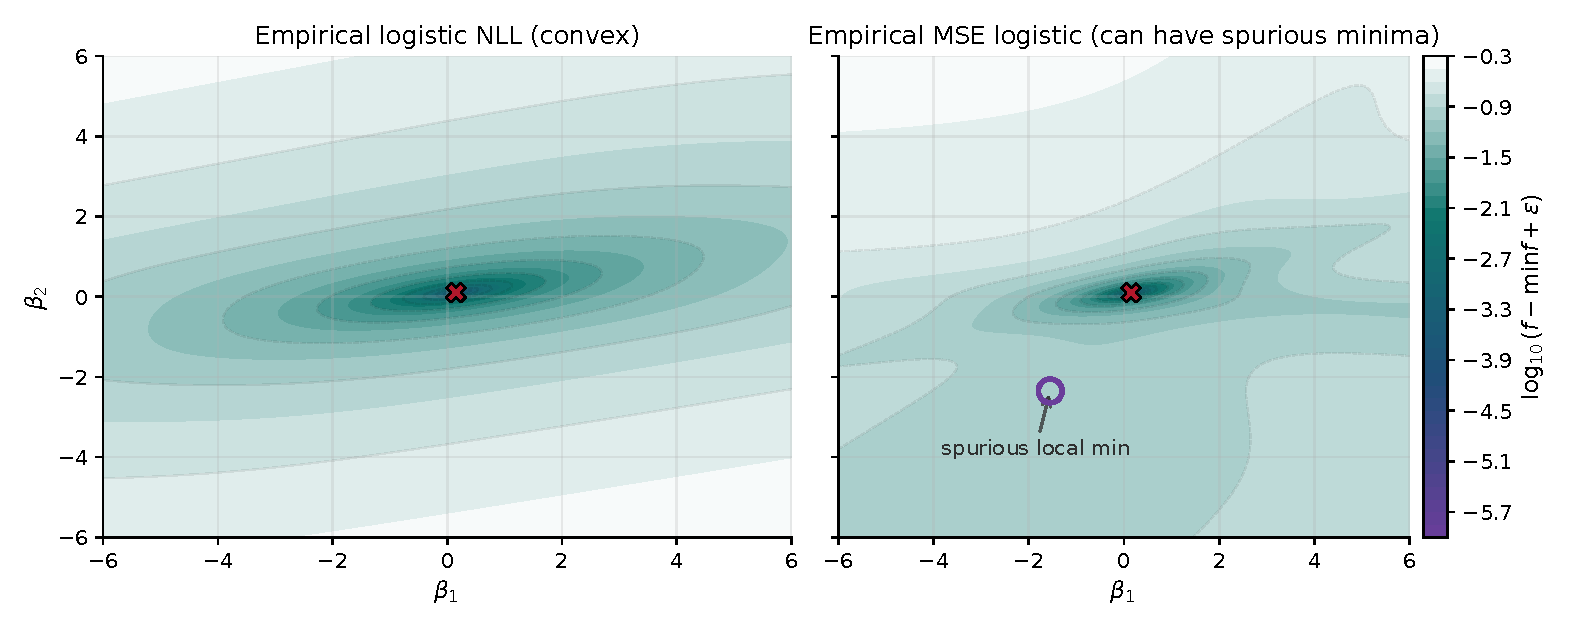
\includegraphics[width=\textwidth]{figures/handouts/convexity_optimization/fig_logistic_empirical_spurious}
  \caption{Empirical logistic landscapes on the dataset in \Cref{ex:logistic-empirical-spurious}.
  The plots show $\log_{10}(f-\min f+\varepsilon)$ for each objective.
  The red X marks the global minimizer in each panel.
  Left: the NLL is convex (one basin).
  Right: the squared-loss objective can have a spurious local minimum (circled), so a local method can get stuck.}
  \label{fig:logistic-empirical-spurious}
\end{figure}

\begin{figure}[t]
  \centering
  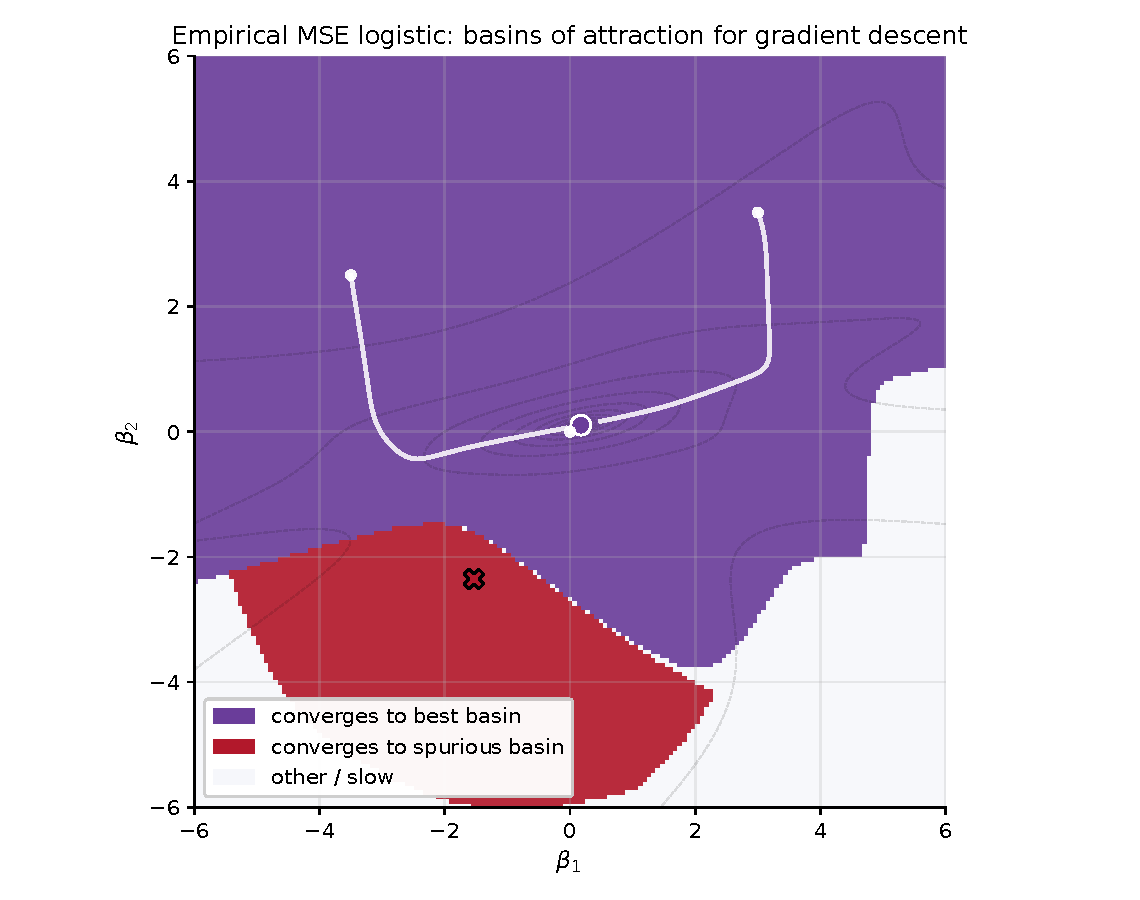
\includegraphics[width=0.92\textwidth]{figures/handouts/convexity_optimization/fig_logistic_empirical_basins}
  \caption{Basins of attraction for gradient descent on the empirical MSE-logistic objective in \Cref{ex:logistic-empirical-spurious}.
  The purple dot and red X mark the two local minimizers.
  Each initialization is colored by which local minimizer fixed-step GD (with $\eta=0.6$) converges to, and the overlaid paths show a few representative trajectories.}
  \label{fig:logistic-empirical-basins}
\end{figure}

Now assume a realizable population model:
\[
Y\mid X=x \sim \mathrm{Bernoulli}(p^\star(x)),
\qquad
p^\star(x) = \sigma(x^\top\beta^\star).
\]
Then the expected squared loss decomposes as
\[
\E\big[(Y-\sigma(X^\top\beta))^2\mid X\big]
= p^\star(X)(1-p^\star(X)) + \big(p^\star(X)-\sigma(X^\top\beta)\big)^2,
\]
so (up to an additive constant) the population objective becomes
\begin{equation}
R(\beta) = \E\big[(\sigma(X^\top\beta)-\sigma(X^\top\beta^\star))^2\big].
\label{eq:logistic-pop-risk}
\end{equation}

\begin{proposition}[One-point monotonicity in the realizable population squared-loss risk]
\label{prop:logistic-pop-one-point}
Assume $\E[\norm{X}_2]<\infty$, and let $R$ be as in \eqref{eq:logistic-pop-risk}. Then for all $\beta$,
\begin{equation}
\ip{\nabla R(\beta)}{\beta-\beta^\star} \ge 0.
\label{eq:one-point}
\end{equation}
In particular, along any ray $\beta(t)=\beta^\star+t(\beta-\beta^\star)$, the function $t\mapsto R(\beta(t))$ is nondecreasing for $t\ge 0$.
\end{proposition}

The next exercise isolates the population monotonicity calculation; structurally it plays the same role as the first-order convexity arguments in the Optimization unit.
\begin{exercise}[One-point monotonicity for realizable MSE-logistic]
\label{ex:logistic-one-point}
Prove \Cref{prop:logistic-pop-one-point}.
Let $\eta=X^\top\beta$ and $\eta^\star=X^\top\beta^\star$.
\begin{enumerate}[leftmargin=*]
  \item Differentiate under the expectation in \eqref{eq:logistic-pop-risk} to show that
  \[
  \nabla R(\beta)
  =2\,\E\Big[(\sigma(\eta)-\sigma(\eta^\star))\,\sigma'(\eta)\,X\Big].
  \]
  \item Show that
  \[
  \ip{\nabla R(\beta)}{\beta-\beta^\star}
  =2\,\E\Big[\sigma'(\eta)\,(\sigma(\eta)-\sigma(\eta^\star))(\eta-\eta^\star)\Big],
  \]
  and conclude it is nonnegative using only that $\sigma$ is increasing and $\sigma'\ge 0$.
  \item Deduce the ray-monotonicity statement by differentiating $g(t)=R(\beta^\star+t(\beta-\beta^\star))$.
\end{enumerate}
\end{exercise}

\SolutionBox[14]{%
\emph{Part (1).}
Differentiate \eqref{eq:logistic-pop-risk} under the expectation:
\[
R(\beta)=\E\big[(\sigma(X^\top\beta)-\sigma(X^\top\beta^\star))^2\big].
\]
Using the chain rule, $\nabla_\beta\sigma(X^\top\beta)=\sigma'(X^\top\beta)\,X$, hence
\[
\nabla R(\beta)
=2\,\E\Big[(\sigma(\eta)-\sigma(\eta^\star))\,\sigma'(\eta)\,X\Big],
\qquad
\eta=X^\top\beta,\ \eta^\star=X^\top\beta^\star.
\]

\emph{Part (2).}
Take the inner product with $(\beta-\beta^\star)$ and use $\ip{X}{\beta-\beta^\star}=\eta-\eta^\star$:
\[
\ip{\nabla R(\beta)}{\beta-\beta^\star}
=2\,\E\Big[\sigma'(\eta)\,(\sigma(\eta)-\sigma(\eta^\star))(\eta-\eta^\star)\Big].
\]
Since $\sigma'(\eta)\ge 0$ and $\sigma$ is increasing, we have
$(\sigma(\eta)-\sigma(\eta^\star))(\eta-\eta^\star)\ge 0$ pointwise.
Therefore the integrand is pointwise nonnegative, and the expectation is nonnegative as claimed.

\emph{Part (3) (ray monotonicity).}
For the ray $\beta(t)=\beta^\star+t(\beta-\beta^\star)$, define $g(t)=R(\beta(t))$.
By the chain rule,
\[
g'(t)=\ip{\nabla R(\beta(t))}{\beta-\beta^\star}\ge 0,
\]
so $t\mapsto R(\beta(t))$ is nondecreasing for $t\ge 0$.
(The argument uses only that the link is increasing with nonnegative derivative, so it holds for any such link function.)%
}

\begin{corollary}[Realizable population MSE-logistic has no spurious local minima]
\label{cor:logistic-pop-no-spurious}
Under the assumptions of \Cref{prop:logistic-pop-one-point}, every local minimizer of the realizable population risk $R$ in \eqref{eq:logistic-pop-risk} is global.
If in addition $\E[XX^\top]\succ 0$, then the unique global minimizer is $\beta^\star$.
\end{corollary}

\begin{exercise}[Stationarity + one-point monotonicity $\Rightarrow$ no spurious local minima]
\label{ex:logistic-one-point-no-spurious}
Prove \Cref{cor:logistic-pop-no-spurious} from \Cref{prop:logistic-pop-one-point}.
\begin{enumerate}[leftmargin=*]
  \item Let $\bar\beta$ be a local minimizer. Since $R$ is differentiable, $\nabla R(\bar\beta)=0$.
  Combine this with \Cref{eq:one-point} to show that
  \[
    0
    = \ip{\nabla R(\bar\beta)}{\bar\beta-\beta^\star}
    = 2\,\E\Big[\sigma'(\bar\eta)\,(\sigma(\bar\eta)-\sigma(\eta^\star))(\bar\eta-\eta^\star)\Big],
  \]
  where $\bar\eta=X^\top\bar\beta$ and $\eta^\star=X^\top\beta^\star$.
  Conclude that $\sigma(X^\top\bar\beta)=\sigma(X^\top\beta^\star)$ almost surely.
  \item Deduce that $R(\bar\beta)=0$, so $\bar\beta$ is a global minimizer.
  \item For uniqueness: show that if $R(\beta)=0$, then $X^\top(\beta-\beta^\star)=0$ almost surely, and deduce $\beta=\beta^\star$ under $\E[XX^\top]\succ 0$.
\end{enumerate}
\end{exercise}

\SolutionBox[14]{%
\emph{Part (1).}
Let $\bar\beta$ be a local minimizer of the differentiable function $R$.
Then $\nabla R(\bar\beta)=0$.
Applying \Cref{prop:logistic-pop-one-point} at $\beta=\bar\beta$ gives
\[
0
= \ip{\nabla R(\bar\beta)}{\bar\beta-\beta^\star}
= 2\,\E\Big[\sigma'(\bar\eta)\,(\sigma(\bar\eta)-\sigma(\eta^\star))(\bar\eta-\eta^\star)\Big],
\qquad \bar\eta=X^\top\bar\beta,\ \eta^\star=X^\top\beta^\star.
\]
The integrand is pointwise nonnegative because $\sigma'(\bar\eta)\ge 0$ and $\sigma$ is increasing, so the expectation can vanish only if the integrand is zero almost surely.
Since $\sigma'(z)>0$ for every finite $z$, this implies
\[
(\sigma(\bar\eta)-\sigma(\eta^\star))(\bar\eta-\eta^\star)=0
\qquad\text{almost surely.}
\]
Because $\sigma$ is strictly increasing, the product above is zero if and only if $\bar\eta=\eta^\star$, equivalently $\sigma(X^\top\bar\beta)=\sigma(X^\top\beta^\star)$ almost surely.

\emph{Part (2).}
If $\sigma(X^\top\bar\beta)=\sigma(X^\top\beta^\star)$ almost surely, then the integrand in \eqref{eq:logistic-pop-risk} vanishes almost surely, so
\[
R(\bar\beta)=\E\big[(\sigma(X^\top\bar\beta)-\sigma(X^\top\beta^\star))^2\big]=0.
\]
Since $R(\beta^\star)=0$ as well, $\bar\beta$ is a global minimizer.

\emph{Part (3) (uniqueness).}
If $R(\beta)=0$, then
\[
\E\big[(\sigma(X^\top\beta)-\sigma(X^\top\beta^\star))^2\big]=0,
\]
so $\sigma(X^\top\beta)=\sigma(X^\top\beta^\star)$ almost surely.
Since $\sigma$ is strictly increasing, this implies $X^\top(\beta-\beta^\star)=0$ almost surely.
Taking expectations yields
$(\beta-\beta^\star)^\top\E[XX^\top](\beta-\beta^\star)=0$.
If $\E[XX^\top]\succ 0$, then the quadratic form is strictly positive unless $\beta=\beta^\star$, so $\beta^\star$ is the unique global minimizer.%
}

The population MSE-logistic risk is nonconvex, but it still has the simple geometry that moving away from $\beta^\star$ does not help along any ray from $\beta^\star$.
This is qualitatively different from objectives like ecological logistic regression (\Cref{sec:ecological-logistic}), where aggregation introduces intrinsic nonconvexity and the landscape can have many distinct basins even under a clean population model.

Even with this benign global geometry, gradient descent can be slow because of saturation and flat plateaus.
The one-point monotonicity in \Cref{prop:logistic-pop-one-point} is a global geometry guarantee, but it is not a rate guarantee.
Far from $\beta^\star$, the squared-loss logistic objective can become very flat because the logistic link saturates:
$\sigma(z)\to 0$ or $1$ and $\sigma'(z)\to 0$ as $|z|\to\infty$.
The squared-loss gradient carries a factor of $\sigma'(X^\top\beta)$, so when the model is very confident (large $|X^\top\beta|$), the gradient can be tiny even if the objective value is not close to its minimum.
This mirrors the ``confidence weights'' story for convex NLL objectives:
in logistic NLL, curvature is largest near the decision boundary, while very confident points contribute little.
For squared loss, that same saturation suppresses the \emph{descent signal} itself, producing plateaus where $\norm{\nabla R(\beta)}_2$ is small even though $R(\beta)-R(\beta^\star)$ is not.

\begin{proposition}[Realizable squared-loss logistic: arbitrarily flat far from $\beta^\star$]
\label{prop:logistic-pop-flat}
Assume $\E[\norm{X}_2]<\infty$ and let $R$ be the realizable population risk \eqref{eq:logistic-pop-risk}.
Define $g(t)=R(t\beta^\star)$ for $t\ge 1$.
Then:
\begin{enumerate}[leftmargin=*]
  \item $g$ is nondecreasing on $[1,\infty)$ and converges to a finite limit $g(\infty)$.
  \item $\lim_{t\to\infty} g'(t)=0$ and $\lim_{t\to\infty}\norm{\nabla R(t\beta^\star)}_2=0$.
  \item If $\Pr(X^\top\beta^\star\neq 0)>0$, then $g(\infty)>0$.
\end{enumerate}
In particular, there are directions along which the landscape becomes arbitrarily flat even though the excess risk stays bounded away from $0$.
\end{proposition}

\emph{Proof idea.} See Exercise~\ref{ex:logistic-plateau}.

\begin{exercise}[Prove the plateau]
\label{ex:logistic-plateau}
In the realizable population model, let $g(t)=R(t\beta^\star)$ for $t\ge 1$.
\begin{enumerate}[leftmargin=*]
  \item Show that
  \[
    g'(t)=2\,\E\big[(\sigma(t\eta^\star)-\sigma(\eta^\star))\,\sigma'(t\eta^\star)\,\eta^\star\big],
    \qquad \eta^\star=X^\top\beta^\star,
  \]
  and conclude that $g$ is nondecreasing (hence $g(t)\to g(\infty)$ since $0\le g(t)\le 1$).
  \item Show that $g'(t)\to 0$ and $\nabla R(t\beta^\star)\to 0$ as $t\to\infty$.
  Interpret this as: \emph{without} a PL/strong-convexity-type condition, small gradient does not imply near-optimality.
  \item Assume $\Pr(\eta^\star\neq 0)>0$.
  Show that $g(\infty)>0$.
\end{enumerate}
\end{exercise}

\SolutionBox[12]{%
Write $\eta^\star=X^\top\beta^\star$ so that $g(t)=\E[(\sigma(t\eta^\star)-\sigma(\eta^\star))^2]$.

\emph{Part (1).}
Differentiate under the expectation:
by the chain rule,
\[
\frac{d}{dt}\sigma(t\eta^\star)=\sigma'(t\eta^\star)\,\eta^\star,
\]
so
\[
g'(t)
=\E\Big[2(\sigma(t\eta^\star)-\sigma(\eta^\star))\cdot \sigma'(t\eta^\star)\,\eta^\star\Big]
=2\,\E\big[(\sigma(t\eta^\star)-\sigma(\eta^\star))\,\sigma'(t\eta^\star)\,\eta^\star\big].
\]
For $t\ge 1$, $\sigma(t\eta^\star)-\sigma(\eta^\star)$ has the same sign as $(t-1)\eta^\star$ since $\sigma$ is increasing.
Because $\sigma'\ge 0$, the integrand is pointwise nonnegative, hence $g'(t)\ge 0$ and $g$ is nondecreasing.
Since $g(t)\in[0,1]$, it follows that $g(t)\to g(\infty)$ for some finite limit $g(\infty)$.

\emph{Part (2).}
For each fixed $\eta^\star\neq 0$, we have $t\eta^\star\to \pm\infty$ and therefore $\sigma'(t\eta^\star)\to 0$ as $t\to\infty$.
Also,
\[
\big|(\sigma(t\eta^\star)-\sigma(\eta^\star))\,\sigma'(t\eta^\star)\,\eta^\star\big|
\le \sigma'(0)\,|\eta^\star|
\le \sigma'(0)\,\norm{\beta^\star}_2\,\norm{X}_2,
\]
which is integrable since $\E[\norm{X}_2]<\infty$.
We will use the following standard fact: if random variables $Z_t$ satisfy $|Z_t|\le W$ with $\E[W]<\infty$ and $Z_t\to 0$ almost surely, then $\E[Z_t]\to 0$.
Applying this fact here gives $g'(t)\to 0$ as $t\to\infty$.

\smallskip
Similarly, differentiating \eqref{eq:logistic-pop-risk} gives
\[
\nabla R(t\beta^\star)
=2\,\E\big[(\sigma(t\eta^\star)-\sigma(\eta^\star))\,\sigma'(t\eta^\star)\,X\big].
\]
The integrand norm is bounded by $2\sigma'(0)\norm{X}_2$, and for each fixed $X$ the factor $\sigma'(t\eta^\star)$ tends to $0$ (or the bracketed term vanishes when $\eta^\star=0$), so the same reasoning lets us pass the limit through the expectation and conclude $\nabla R(t\beta^\star)\to 0$.

\emph{Part (3).}
As $t\to\infty$ we have $\sigma(t\eta^\star)\to 1$ when $\eta^\star>0$, $\sigma(t\eta^\star)\to 0$ when $\eta^\star<0$, and $\sigma(t\eta^\star)=\sigma(\eta^\star)=1/2$ when $\eta^\star=0$.
Since $0\le (\sigma(t\eta^\star)-\sigma(\eta^\star))^2\le 1$, we can apply the same fact (with $W=1$) to pass the limit through the expectation and obtain
\[
g(\infty)=\E\Big[(1-\sigma(\eta^\star))^2\mathbf{1}\{\eta^\star>0\} + \sigma(\eta^\star)^2\mathbf{1}\{\eta^\star<0\}\Big].
\]
If $\Pr(\eta^\star\neq 0)>0$, then the integrand is strictly positive on $\{\eta^\star\neq 0\}$, so $g(\infty)>0$.

Along this ray, the risk can remain bounded away from $0$ while the gradient (and directional derivative) goes to $0$.
Without a condition like PL/strong convexity, a small gradient does not by itself certify near-optimality.
}

Conditions like strong convexity or the PL inequality (\Cref{def:pl-inequality}) prevent this phenomenon: they rule out large flat regions away from the optimum by relating gradient size to suboptimality.
\Cref{prop:logistic-pop-flat} shows the realizable squared-loss logistic risk does not have such a global guarantee in general.

In the realizable population model, the one-point monotonicity in \Cref{prop:logistic-pop-one-point} is a \emph{global} geometric statement.
To get an actual rate for gradient descent, we also need a \emph{local curvature} condition near $\beta^\star$.
One simple sufficient condition is bounded features, which implies local strong convexity (hence a linear rate) around the optimum.

\begin{proposition}[Local linear convergence of gradient descent near $\beta^\star$]
\label{prop:logistic-pop-local-rate}
Assume $\E[XX^\top]\succeq \lambda I_d$ and $\norm{X}_2\le R$ almost surely for some $\lambda,R>0$.
Then at $\beta^\star$,
\[
\Hess R(\beta^\star)\succeq m_0 I_d,
\qquad
m_0 = 2\,\sigma'(R\norm{\beta^\star}_2)^2\,\lambda,
\]
and there exist $r>0$ and constants $0<m\le L<\infty$ such that the population risk $R$ in \eqref{eq:logistic-pop-risk} is $m$-strongly convex and $L$-smooth on the ball $\{\beta:\ \norm{\beta-\beta^\star}_2\le r\}$.
Consequently, gradient descent with step size $1/L$ initialized in this ball satisfies
\[
R(\beta^{(k)})-R(\beta^\star)
\le \left(1-\frac{m}{L}\right)^k\bigl(R(\beta^{(0)})-R(\beta^\star)\bigr)
\qquad\text{(see \citealp[\S9.3]{boyd_vandenberghe_2004_convex}).}
\]
\end{proposition}

\begin{proof}
Differentiate \eqref{eq:logistic-pop-risk} twice.
At $\beta=\beta^\star$, the cross term vanishes and the Hessian simplifies to
\[
\Hess R(\beta^\star)=2\,\E\big[\sigma'(X^\top\beta^\star)^2\,XX^\top\big].
\]
Since $\norm{X^\top\beta^\star}\le \norm{X}_2\norm{\beta^\star}_2\le R\norm{\beta^\star}_2$ almost surely, we have
$\sigma'(X^\top\beta^\star)\ge \sigma'(R\norm{\beta^\star}_2)>0$ almost surely (since $\sigma'$ is even and decreases with $|z|$), hence
\[
\Hess R(\beta^\star)\succeq 2\,\sigma'(R\norm{\beta^\star}_2)^2\,\E[XX^\top]\succeq 2\,\sigma'(R\norm{\beta^\star}_2)^2\,\lambda I_d.
\]
This is the claimed bound with $m_0=2\,\sigma'(R\norm{\beta^\star}_2)^2\,\lambda$.
Because $R$ is twice continuously differentiable and $\norm{X}_2\le R$ almost surely, $\Hess R(\beta)$ varies continuously in $\beta$ and is bounded on compact sets.
Therefore, on a sufficiently small ball around $\beta^\star$, the Hessian is bounded below by (say) $\tfrac12 m_0 I_d$ and above by $L I_d$ for some finite $L$, which gives local strong convexity and smoothness.
The linear convergence rate for gradient descent on an $m$-strongly convex and $L$-smooth function is standard (cited above).
\end{proof}

Under misspecification, hard multimodality can return.
If $p^\star(x)$ is not representable as $\sigma(x^\top\beta)$ (e.g.\ marginalizing over latent classes can yield mixtures of logits), then \eqref{eq:one-point} need not hold, and the population squared-loss risk can become bimodal with spurious local minima.
Benign global geometry often hinges on model and data assumptions.
This is one reason MLE (convex NLL) is often more stable than squared-loss fitting in logistic-type binary regression models.

\begin{example}[Misspecification can create a spurious local minimum for squared-loss logistic regression]
\label{ex:logistic-misspecified-spurious}
Consider a 1D feature $X$ that takes values $\{-2,-1,1,2\}$ with equal probability, and parameterize $\beta=(\beta_0,\beta_1)$ so that $q_\beta(x)=\sigma(\beta_0+\beta_1 x)$.
Let the true conditional probabilities be
\[
p^\star(-2)=0.49,\quad p^\star(-1)=0.87,\quad p^\star(1)=0.92,\quad p^\star(2)=0.36.
\]
This $p^\star$ is not representable as $q_\beta$, since it is not monotone in $x$.

For the population squared-loss risk $R_{\mathrm{MSE}}(\beta)=\E[(q_\beta(X)-p^\star(X))^2]$, a direct evaluation shows two distinct basins:
numerically, evaluating $R_{\mathrm{MSE}}$ on a grid reveals a global minimizer and a spurious local minimizer.
See \Cref{fig:logistic-landscape-2d}.
\end{example}

\begin{figure}[t]
  \centering
  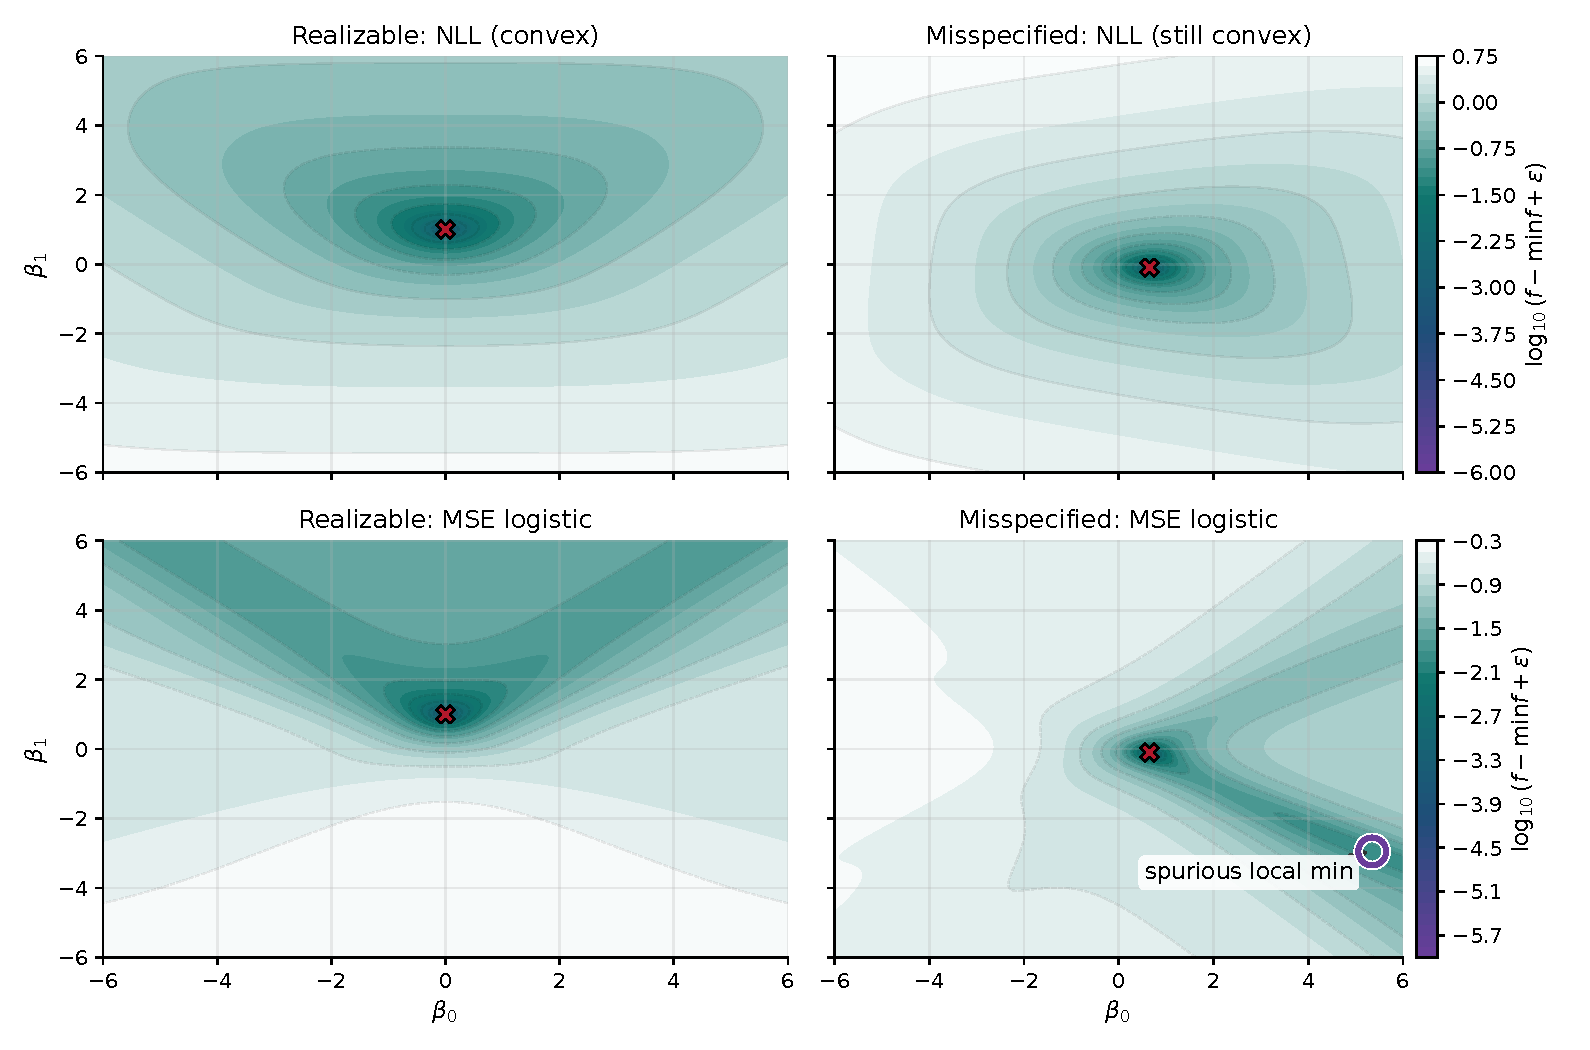
\includegraphics[width=\textwidth]{figures/handouts/convexity_optimization/fig_logistic_landscape_2d}
  \caption{A consistent contourf view of logistic landscapes in a 2D parameterization $\beta=(\beta_0,\beta_1)$.
  The plots show $\log_{10}(f-\min f+\varepsilon)$ for each objective, which makes basins comparable across panels.
  The red X marker indicates the global minimizer in each panel; in the bottom-right plot, the circled point is a spurious local minimum.
  In this example, the NLL landscape is unimodal in both realizable and misspecified settings, while the squared-loss landscape can develop extra basins under misspecification.}
  \label{fig:logistic-landscape-2d}
\end{figure}

% ------------------------------------------------------------
Example~I separates three distinct regimes.
Empirical MSE-logistic can create spurious basins; the realizable population risk has no spurious local minima but can still be slow because of broad plateaus; and misspecification can bring back genuinely wrong stable basins.
The response depends on the regime: use a stable objective when possible, use damping or line search when curvature is unreliable, and use restarts or stronger initializations when multiple basins are present.

% ------------------------------------------------------------
\section[Example II (phase retrieval)]{Example II: multimodality from symmetry, but only global optima in phase retrieval}
\label{sec:phase-retrieval}

In coherent diffraction imaging, optics, and astronomy, sensors measure intensities and lose phase.
A canonical real model is \emph{phase retrieval}:
\[
y_i = (a_i^\top x^\star)^2,\qquad i=1,\dots,m,
\]
where $x^\star\in\R^d$ is the unknown signal and $a_i$ are known sensing vectors.
A standard nonconvex least-squares objective is
\begin{equation}
F(x)=\frac{1}{4m}\sum_{i=1}^m\big((a_i^\top x)^2 - y_i\big)^2.
\label{eq:phase-empirical}
\end{equation}
This objective is nonconvex for structural reasons (it involves squares of linear forms),
and it is \emph{inherently} multimodal because $x^\star$ and $-x^\star$ generate the same data.

Like squared-loss logistic regression, phase retrieval is a smooth, nonconvex least-squares objective.
But here the nonconvexity is driven primarily by a \emph{symmetry}: $x^\star$ and $-x^\star$ generate the same data.
In population (for Gaussian designs), this symmetry produces multiple global optima but \emph{no} suboptimal local minima; the remaining stationary points are saddles.
This is ``benign'' nonconvexity (a strict-saddle picture), and it contrasts with ecological logistic regression (\Cref{sec:ecological-logistic}), where aggregation creates intrinsic nonconvexity and can lead to many distinct basins.
This ``benign geometry'' picture (multiple equivalent global minimizers; strict saddles elsewhere) appears broadly in modern tractable nonconvex problems; see \citet[\S2]{sun_qu_wright_2015_nonconvex_not_scary} and \citet[\S1]{zhang_qu_wright_2020_symmetry_geometry}.

\begin{figure}[t]
  \centering
  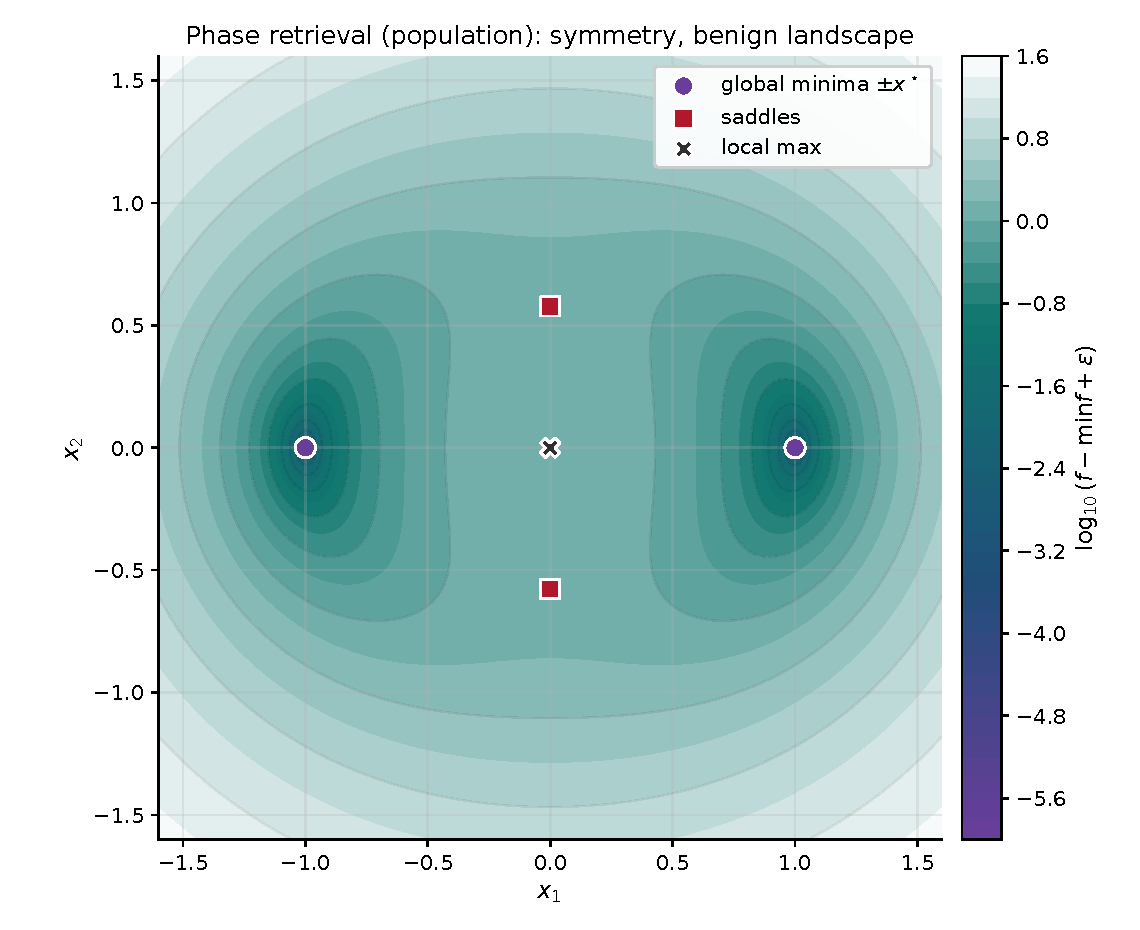
\includegraphics[width=0.86\textwidth]{figures/handouts/convexity_optimization/fig_phase_retrieval_landscape}
  \caption{Population phase retrieval in $d=2$: the landscape is nonconvex and symmetric ($x\sim -x$), but the only local minima are the two global minima $\pm x^\star$; other critical points are saddles or a local maximum at the origin.}
  \label{fig:phase-retrieval-landscape}
\end{figure}

For a clean population model, assume $a\sim N(0,I_d)$ and consider the \emph{population} objective
\begin{equation}
  f(x)=\frac12\,\E\Big[\big((a^\top x)^2 - (a^\top x^\star)^2\big)^2\Big].
  \label{eq:phase-pop}
\end{equation}

\begin{proposition}[Population phase retrieval: nonconvex but no spurious local minima]
\label{prop:phase-retrieval-benign}
For $f$ in \eqref{eq:phase-pop},
\begin{equation}
  f(x)
  =\frac{3}{2}\norm{x}^4 - \norm{x}^2\norm{x^\star}^2 - 2\ip{x}{x^\star}^2 + \frac{3}{2}\norm{x^\star}^4,
  \label{eq:phase-pop-closed-form}
\end{equation}
and the stationary points are:
\begin{enumerate}[leftmargin=*]
  \item global minima $x=\pm x^\star$ (value $0$),
  \item a local maximum at $x=0$,
  \item a saddle set $\{x:\ x\perp x^\star,\ \norm{x}=\norm{x^\star}/\sqrt{3}\}$.
\end{enumerate}
In particular, every local minimum is global.
\end{proposition}

\begin{exercise}[Phase retrieval: derive and classify the population stationary points]
\label{ex:phase-pop-derivation}
Prove \Cref{prop:phase-retrieval-benign}.
\begin{enumerate}[leftmargin=*]
  \item Expand \eqref{eq:phase-pop} and use the Gaussian fourth-moment identities
  \[
  \E[(a^\top u)^4]=3\norm{u}^4,
  \qquad
  \E[(a^\top u)^2(a^\top v)^2]=\norm{u}^2\norm{v}^2 + 2\ip{u}{v}^2,
  \]
  to obtain \eqref{eq:phase-pop-closed-form}.
  \item Differentiate \eqref{eq:phase-pop-closed-form} to get an explicit formula for $\nabla f(x)$.
  \item Solve $\nabla f(x)=0$ by decomposing $x=\alpha x^\star + u$ with $u\perp x^\star$.
  \item Classify the stationary points as global minima, a local maximum, and a saddle set.
\end{enumerate}
\end{exercise}

\SolutionBox[22]{%
\emph{Part (1) (closed form).}
Expanding the square in \eqref{eq:phase-pop} gives
\[
f(x)
=\frac12\,\E\big[(a^\top x)^4\big]
\;-\;\E\big[(a^\top x)^2(a^\top x^\star)^2\big]
\;+\;\frac12\,\E\big[(a^\top x^\star)^4\big].
\]
Apply the stated Gaussian fourth-moment identities with $u=x$ and $v=x^\star$ to get
\[
\E[(a^\top x)^4]=3\norm{x}^4,\qquad
\E[(a^\top x^\star)^4]=3\norm{x^\star}^4,
\]
and
\[
\E[(a^\top x)^2(a^\top x^\star)^2]=\norm{x}^2\norm{x^\star}^2 + 2\ip{x}{x^\star}^2.
\]
Substituting yields \eqref{eq:phase-pop-closed-form}.

\emph{Part (2) (gradient).}
Differentiate \eqref{eq:phase-pop-closed-form}:
\[
\nabla f(x)
= 6\norm{x}^2 x - 2\norm{x^\star}^2 x - 4\ip{x}{x^\star}x^\star
= (6\norm{x}^2-2\norm{x^\star}^2)x - 4\ip{x}{x^\star}x^\star.
\]

\emph{Part (3) (stationary points).}
Let $r=\norm{x^\star}_2$ and decompose $x=\alpha x^\star + u$ with $u\perp x^\star$.
Then $\ip{x}{x^\star}=\alpha r^2$ and $\norm{x}^2=\alpha^2r^2+\norm{u}^2$.
Setting $\nabla f(x)=0$ and matching the $u$ and $x^\star$ components gives
\[
(6\norm{x}^2-2r^2)\,u=0,
\qquad
\alpha\,(6\norm{x}^2-6r^2)=0.
\]
If $u=0$, then either $\alpha=0$ (so $x=0$) or $\norm{x}^2=r^2$ (so $\alpha=\pm 1$ and $x=\pm x^\star$).
If $u\neq 0$, then the first equation forces $\norm{x}^2=r^2/3$, and the second forces $\alpha=0$, hence
$x\perp x^\star$ and $\norm{x}=r/\sqrt{3}$.
This gives exactly the stationary-point list in \Cref{prop:phase-retrieval-benign}.

\emph{Part (4) (classification).}
Since $f$ in \eqref{eq:phase-pop} is an expectation of a square, $f(x)\ge 0$ for all $x$.
Also $f(\pm x^\star)=0$, so $\pm x^\star$ are global minima.

For $x=0$, the expansion \eqref{eq:phase-pop-closed-form} shows
\[
f(0)-f(x)= r^2\norm{x}^2 + 2\ip{x}{x^\star}^2 - \frac{3}{2}\norm{x}^4,
\]
which is strictly positive for all sufficiently small $x\neq 0$ (the quadratic term dominates), so $x=0$ is a local maximum.

Finally, if $x\perp x^\star$ and $\norm{x}=r/\sqrt{3}$, then the univariate restriction $t\mapsto f(x+t x^\star)$ has negative second derivative at $t=0$, so there is a direction of negative curvature.
Hence these points are saddles, and every local minimum is global.%
}

This is symmetry-driven nonconvexity with a strict-saddle geometry:
every non-optimal stationary point has a direction of negative curvature.

Phase retrieval is typically approached via the two-stage template in \Cref{alg:two-stage-template}:
use a cheap global initializer, then run a local method.
In the Gaussian model, there is a clean way to build a provably good direction estimate from a simple moment identity.
Assume the noiseless Gaussian design model $a_i \stackrel{\mathrm{iid}}{\sim} N(0,I_d)$ with measurements $y_i=(a_i^\top x^\star)^2$.
Define the \emph{spectral matrix}
\[
  Y = \frac{1}{m}\sum_{i=1}^m y_i a_i a_i^\top.
\]
Also define the radius estimate
\[
  \hat r^2 = \frac{1}{m}\sum_{i=1}^m y_i,
\]
which satisfies $\E[\hat r^2]=\norm{x^\star}_2^2$.
If $\hat u$ is a unit-norm top eigenvector of $Y$, then the standard spectral initializer is $x^{(0)}=\hat r\,\hat u$.

The next proposition explains why this initialization is reasonable.
It shows that (i) the population matrix $\E[Y]$ has a unique leading eigenvector in the $x^\star$ direction, and (ii) if the empirical $Y$ is close to $\E[Y]$ in operator norm then its leading eigenvector must be close to $\pm x^\star/\norm{x^\star}_2$.
(Here $\norm{M}_{\mathrm{op}}$ denotes the operator norm, i.e.\ the largest absolute eigenvalue for a symmetric matrix $M$.)

\begin{proposition}[Gaussian phase retrieval: why the spectral initializer points at $x^\star$]
\label{prop:phase-spectral-init}
Assume $x^\star\neq 0$, let $a\sim N(0,I_d)$, and set $y=(a^\top x^\star)^2$.
Write $r=\norm{x^\star}_2$ and $u^\star=x^\star/r$.
Define the population matrix
\[
  Y_{\mathrm{pop}} = \E\big[y\,a a^\top\big]
  = \E\big[(a^\top x^\star)^2 a a^\top\big].
\]
Then
\[
  Y_{\mathrm{pop}}=r^2 I_d + 2x^\star(x^\star)^\top,
\]
so the unique leading eigenvector of $Y_{\mathrm{pop}}$ is $u^\star$.
Moreover, if $Y$ is any symmetric matrix satisfying
\[
\norm{Y-Y_{\mathrm{pop}}}_{\mathrm{op}} \le \varepsilon\, r^2
\qquad\text{for some }\varepsilon\in(0,1),
\]
then for every unit-norm leading eigenvector $\hat u$ of $Y$ there exists a sign $s\in\{\pm 1\}$ such that
$\norm{\hat u-su^\star}_2\le \sqrt{2\varepsilon}$.
\end{proposition}

\begin{exercise}[Phase retrieval: why spectral initialization points at $x^\star$]
\label{ex:phase-spectral-spike}
Prove \Cref{prop:phase-spectral-init}.
Conclude that if the empirical matrix $Y$ is close to $Y_{\mathrm{pop}}$ in operator norm, then its top eigenvector is close to $\pm u^\star$ and the spectral initializer $x^{(0)}=\hat r\,\hat u$ is close to $\pm x^\star$.
\emph{Hint:} to compute $Y_{\mathrm{pop}}$, you can either compute entries using the Gaussian fourth-moment identity
$\E[a_i a_j a_k a_\ell]=\delta_{ij}\delta_{k\ell}+\delta_{ik}\delta_{j\ell}+\delta_{i\ell}\delta_{jk}$,
or compute the entries directly by expanding.
For the perturbation bound, compare quadratic forms $v^\top Y v$ and use $|v^\top (Y-Y_{\mathrm{pop}}) v|\le \norm{Y-Y_{\mathrm{pop}}}_{\mathrm{op}}$ for unit $v$.
Finally, explain in a sentence why one expects $\norm{Y-Y_{\mathrm{pop}}}_{\mathrm{op}}$ to be small when $m$ is large in the Gaussian model.
\end{exercise}

\SolutionBox[20]{%
Write $u=x^\star$ and expand $y=(a^\top u)^2=\sum_{k,\ell} u_k u_\ell a_k a_\ell$.
For each entry $(i,j)$,
\[
\E\!\big[y\,a_i a_j\big]
=\sum_{k,\ell} u_k u_\ell\,\E[a_i a_j a_k a_\ell]
=\sum_{k,\ell} u_k u_\ell\bigl(\delta_{ij}\delta_{k\ell}+\delta_{ik}\delta_{j\ell}+\delta_{i\ell}\delta_{jk}\bigr).
\]
The first term gives $\delta_{ij}\sum_k u_k^2=\delta_{ij}\norm{u}_2^2$.
The second and third terms each give $u_i u_j$.
Thus $\E[y\,a_i a_j]=\norm{u}_2^2\,\delta_{ij}+2u_i u_j$, i.e.
$Y_{\mathrm{pop}}=\norm{u}_2^2 I_d + 2uu^\top$.

For eigenvalues, note that $Y_{\mathrm{pop}}u=(\norm{u}_2^2+2\norm{u}_2^2)u=3\norm{u}_2^2 u$.
If $w\perp u$, then $uu^\top w=0$ so $Y_{\mathrm{pop}}w=\norm{u}_2^2 w$.
Hence the unique top eigenspace is $\mathrm{span}\{u\}$.

Let $r=\norm{u}_2$ and $u^\star=u/r$.
Let $\hat u$ be a unit top eigenvector of $Y$.
Write $E=Y-Y_{\mathrm{pop}}$ and assume $\norm{E}_{\mathrm{op}}\le \varepsilon r^2$.
Then
\[
\hat u^\top Y_{\mathrm{pop}} \hat u
= \hat u^\top Y \hat u - \hat u^\top E \hat u
\ge \lambda_{\max}(Y) - \norm{E}_{\mathrm{op}}
\ge (u^\star)^\top Y u^\star - \norm{E}_{\mathrm{op}}
\ge 3r^2 - 2\varepsilon r^2.
\]
On the other hand,
$
\hat u^\top Y_{\mathrm{pop}} \hat u
= r^2 + 2r^2\,|\ip{\hat u}{u^\star}|^2.
$
Combining gives $|\ip{\hat u}{u^\star}|^2\ge 1-\varepsilon$.
Choosing the sign that maximizes the inner product,
\[
\min\{\norm{\hat u-u^\star}_2,\norm{\hat u+u^\star}_2\}^2
=2\bigl(1-|\ip{\hat u}{u^\star}|\bigr)
\le 2\bigl(1-|\ip{\hat u}{u^\star}|^2\bigr)
\le 2\varepsilon.
\]

The matrix $Y$ is an empirical average of i.i.d.\ symmetric matrices with mean $Y_{\mathrm{pop}}$.
To make this quantitative in high dimensions, one uses concentration inequalities for random matrices to bound $\norm{Y-Y_{\mathrm{pop}}}_{\mathrm{op}}$ with high probability; see \citet[\S2.2]{zhang_qu_wright_2020_symmetry_geometry} for discussion and references.
These probability tools are largely orthogonal to our focus here.%
}

Once you have an initialization that is close to $\pm x^\star$, the local stage behaves like the convex story again.
In the Gaussian population objective, $\pm x^\star$ are not only global minima: they are \emph{locally strongly convex} minima, so the standard local strong-convexity analysis from the Optimization unit gives a linear rate while the iterates remain in that neighborhood.

\begin{exercise}[Phase retrieval: local convexity near $\pm x^\star$ in the population objective]
\label{ex:phase-pop-local-strong-convex}
For the population objective $f$ in \eqref{eq:phase-pop-closed-form}, compute the Hessian $\Hess f(x)$ and show that
\[
\Hess f(x^\star)=4\norm{x^\star}_2^2 I_d + 8x^\star(x^\star)^\top.
\]
Deduce the eigenvalues of $\Hess f(x^\star)$ and interpret this as a local condition-number statement near $x^\star$.
\end{exercise}

\SolutionBox[12]{%
Differentiate the gradient formula in the solution to \Cref{ex:phase-pop-derivation}:
for $x\in\R^d$,
\[
\Hess f(x)=12xx^\top + (6\norm{x}_2^2-2\norm{x^\star}_2^2)I_d - 4x^\star(x^\star)^\top.
\]
At $x=x^\star$ this becomes
\[
\Hess f(x^\star)=(12-4)x^\star(x^\star)^\top + 4\norm{x^\star}_2^2 I_d
=8x^\star(x^\star)^\top + 4\norm{x^\star}_2^2 I_d.
\]
Along $u^\star=x^\star/\norm{x^\star}_2$ the eigenvalue is $12\norm{x^\star}_2^2$, and along any direction orthogonal to $x^\star$ the eigenvalue is $4\norm{x^\star}_2^2$.
So near $x^\star$ the population objective is well conditioned (local condition number $3$), which is exactly the regime where local methods behave like in the convex case.%
}

These pieces give the standard Gaussian-model story:
spectral initialization supplies a direction close to $\pm x^\star$, and the local geometry near $\pm x^\star$ is strongly convex, so local methods converge quickly once initialized there.
Rigorous finite-sample analyses follow this template; see \citet[\S2.2]{zhang_qu_wright_2020_symmetry_geometry} and references therein.

Phase retrieval shows a different kind of nonconvexity.
The sign symmetry creates multiple optima, but they are equivalent, and the remaining stationary points are saddles rather than bad local minima.
The right response is therefore not exhaustive global search; it is a coarse initializer, such as a spectral method, followed by local refinement inside the basin of $\pm x^\star$.



% ------------------------------------------------------------
\section[Example III (ecological logistic)]{Example III: hard nonconvexity from aggregation in ecological logistic regression}
\label{sec:ecological-logistic}

In some applications we observe covariates at the unit level but only aggregated outcomes.
For example, we might see covariates $x_{g,1},\dots,x_{g,n_g}$ for individuals in a group (a precinct, a cohort, a batch),
but instead of observing the binary outcomes $Y_{g,i}\in\{0,1\}$ we only observe the group total
\[
Z_g = \sum_{i=1}^{n_g} Y_{g,i}.
\]
Many different binary vectors $(Y_{g,1},\dots,Y_{g,n_g})$ can produce the same total $Z_g$, so the likelihood for $\beta$ must marginalize over a large discrete set of latent ``assignments.''

Assume a logistic model at the unit level:
\[
\Pr(Y_{g,i}=1\mid x_{g,i},\beta)=\sigma(x_{g,i}^\top\beta),
\qquad i=1,\dots,n_g,
\]
with conditional independence across $i$ given the covariates.
Write $p_{g,i}(\beta)=\sigma(x_{g,i}^\top\beta)$.
Then $Z_g$ is a sum of independent but non-identically distributed Bernoulli random variables (a Poisson--binomial model), and the marginal likelihood contains $\binom{n_g}{z_g}$ terms.
The resulting negative log-likelihood is typically nonconvex in $\beta$.
This combinatorial marginalization also creates a separate difficulty that is easy to miss if we focus only on the geometry:
when $n_g$ is large, the likelihood term $\Pr(Z_g=z_g\mid x_{g,1},\dots,x_{g,n_g},\beta)$ can be expensive to evaluate repeatedly inside an optimizer.
The naive computation is literally a sum over $\binom{n_g}{z_g}$ assignments (as in \Cref{ex:eco-logistic-nonconvex}), which is intractable for large groups.
This ``optimization + marginalization'' pattern is common in latent-variable models: hard landscapes and expensive objective evaluations can come together.

An empirical negative log-likelihood objective for $G$ independent groups is
\begin{equation}
  f(\beta)
  =
  -\frac{1}{G}\sum_{g=1}^G \log \Pr(Z_g=z_g \mid x_{g,1},\dots,x_{g,n_g},\beta).
  \label{eq:eco-logistic-obj}
\end{equation}
Two edge cases are instructive.
In the special case where the covariates are constant within each group ($x_{g,i}\equiv x_g$), we have
$Z_g\sim \mathrm{Binomial}(n_g,\sigma(x_g^\top\beta))$, and \eqref{eq:eco-logistic-obj} reduces to the usual convex binomial logistic-regression objective from the Optimization unit.
At the other extreme, if $d=1$ with $\beta=(\beta_0,\beta_1)$ and each group contains covariates in $\pm$ pairs (for every $x$ the value $-x$ appears with the same multiplicity), then the marginal likelihood is symmetric in the slope: it is unchanged under $\beta_1\mapsto -\beta_1$.
This kind of symmetry reflects a genuine non-identifiability from totals alone.

\begin{exercise}[Ecological logistic regression: two easy special cases]
\label{ex:eco-logistic-edge-cases}
\begin{enumerate}[leftmargin=*]
  \item Suppose $x_{g,i}\equiv x_g$ within each group.
  Show that $Z_g\sim \mathrm{Binomial}(n_g,\sigma(x_g^\top\beta))$ and conclude that the corresponding negative log-likelihood is convex in $\beta$.
  \item Assume $d=1$ with $\beta=(\beta_0,\beta_1)$ and suppose the multiset $\{x_1,\dots,x_n\}$ is symmetric: for every $x$ it contains $-x$ with the same multiplicity.
  Show that, for every $z$,
  \[
    \Pr(Z=z\mid x_1,\dots,x_n,(\beta_0,\beta_1))
    =
    \Pr(Z=z\mid x_1,\dots,x_n,(\beta_0,-\beta_1)).
  \]
  Conclude that the likelihood for $\beta_1$ is an even function, so the sign of the slope is not identifiable from $Z$ alone in such a balanced design.
\end{enumerate}
\end{exercise}

\SolutionBox[14]{%
\emph{Part (1).}
If $x_{g,i}\equiv x_g$, then conditional on $x_g$ the unit-level outcomes are i.i.d.\ Bernoulli with success probability $\sigma(x_g^\top\beta)$.
Therefore $Z_g=\sum_{i=1}^{n_g}Y_{g,i}\sim \mathrm{Binomial}(n_g,\sigma(x_g^\top\beta))$.
Up to an additive constant (independent of $\beta$), the per-group negative log-likelihood can be written as a function of the scalar $\eta=x_g^\top\beta$:
\[
\ell_g(\beta)
= -z_g\,\eta + n_g\log(1+e^\eta).
\]
Since $\frac{d^2}{d\eta^2}\ell_g(\eta)=n_g\,\sigma'(\eta)\ge 0$, the map $\eta\mapsto \ell_g(\eta)$ is convex.
Composing a convex function with a linear map $\beta\mapsto x_g^\top\beta$ preserves convexity, so $\ell_g$ is convex in $\beta$.
Summing over $g$ preserves convexity, hence the full objective is convex.

\emph{Part (2).}
Write $p_i(\beta_0,\beta_1)=\sigma(\beta_0+\beta_1 x_i)$.
Replacing $\beta_1$ by $-\beta_1$ replaces $p_i$ by $\tilde p_i=\sigma(\beta_0-\beta_1 x_i)$.
By the assumed symmetry of the multiset $\{x_i\}$, the multiset $\{\tilde p_i\}$ is the same as $\{p_i\}$ up to a permutation (each $x$ is paired with $-x$).
But the distribution of $Z=\sum_i Y_i$ depends only on the multiset of success probabilities, not on how they are ordered, so $\Pr(Z=z\mid x_1,\dots,x_n,(\beta_0,\beta_1))=\Pr(Z=z\mid x_1,\dots,x_n,(\beta_0,-\beta_1))$ for every $z$.
Thus the likelihood is an even function of $\beta_1$, which means the sign of the slope is not identifiable from totals in this balanced design.%
}

This example ties directly to the empirical-versus-population theme from Example~I.
There the bad basins can be a finite-sample artifact under benign population geometry; here the nonconvexity is intrinsic, because even under the correct model and infinite data aggregation forces us to marginalize over discrete latent assignments.
That marginalization step is also the bridge to the Expectation--maximization subsection of the Augmented-state optimization unit: once the assignments are latent, the natural algorithmic object is the EM update map, which alternates exact conditional expectations with parameter updates, rather than a single closed-form convex objective.

To emphasize this, it is useful to look at a \emph{population} version of \eqref{eq:eco-logistic-obj}.
Let $X=(x_1,\dots,x_n)$ denote a random group of covariates and let $Z$ be generated from the model under a true parameter $\beta^\star$.
Define the population objective
\[
F(\beta)=\E\big[-\log \Pr(Z\mid X,\beta)\big].
\]
Because the model is correctly specified, $F$ is minimized at (an observationally equivalent version of) $\beta^\star$.
However, as \Cref{fig:eco-logistic-pop-landscape} illustrates, $F$ can still have multiple separated basins and spurious local minima.

\begin{figure}[H]
  \centering
  \input{figures/handouts/convexity_optimization/fig_ecological_logistic_population_landscape}
  \caption{A toy \emph{population} objective for ecological logistic regression in a 2D parameterization $\beta=(\beta_0,\beta_1)$.
  Each group has $n=6$ units and is equally likely to have covariates $(-4,-3,-2,2,3,4)$, $(-3,-1,1,2,3,4)$, or $(-2,-1,1,2,3,4)$ (in $d=1$); outcomes are generated under $\beta^\star=(0.3,1.2)$.
  The plot shows $\log_{10}(F-\min F+\varepsilon)$, as in \Cref{fig:logistic-landscape-2d}; the red X marks $\beta^\star$ and the open circles mark three spurious local minima in this toy example.}
  \label{fig:eco-logistic-pop-landscape}
\end{figure}

\begin{exercise}[Ecological logistic regression: marginalization and nonconvexity]
\label{ex:eco-logistic-nonconvex}
Fix one group with covariates $x_1,\dots,x_n\in\R^d$ and observe $Z=z$.
Let $p_i(\beta)=\sigma(x_i^\top\beta)$.
\begin{enumerate}[leftmargin=*]
  \item Show that
  \[
    \Pr(Z=z\mid x_1,\dots,x_n,\beta)
    =
    \sum_{\substack{S\subseteq\{1,\dots,n\}\\|S|=z}}
    \ \prod_{i\in S} p_i(\beta)\prod_{j\notin S}\bigl(1-p_j(\beta)\bigr).
  \]
  Interpret this as summing over all ways to choose which $z$ units are the successes.
  \item Specialize to $n=2$ and $z=1$ in $d=1$ with covariates $x_1=a$ and $x_2=b$.
  Let $\ell(\beta)$ be the negative log-likelihood $-\log \Pr(Z=1\mid a,b,\beta)$ with no regularization.
  Show that $\ell''(0)=\tfrac12 ab$.
  Conclude that $\ell$ is not convex whenever $ab<0$.
\end{enumerate}
\end{exercise}

\SolutionBox[20]{%
\emph{Part (1).}
Condition on the covariates.
For any binary vector $y=(y_1,\dots,y_n)\in\{0,1\}^n$, conditional independence gives
\[
\Pr(Y_1=y_1,\dots,Y_n=y_n\mid x_1,\dots,x_n,\beta)
=
\prod_{i=1}^n p_i(\beta)^{y_i}\bigl(1-p_i(\beta)\bigr)^{1-y_i}.
\]
The event $\{Z=z\}$ is the union of all assignments $y$ with exactly $z$ ones, so summing over those assignments yields
\[
\Pr(Z=z\mid x_1,\dots,x_n,\beta)
=
\sum_{\substack{y\in\{0,1\}^n\\ \sum_i y_i=z}}
\ \prod_{i=1}^n p_i(\beta)^{y_i}\bigl(1-p_i(\beta)\bigr)^{1-y_i}.
\]
Reindexing the sum by the subset $S=\{i:\ y_i=1\}$ (which has $|S|=z$) gives the stated formula.

\emph{Part (2).}
For $n=2$ and $z=1$, let $p_1(\beta)=\sigma(a\beta)$ and $p_2(\beta)=\sigma(b\beta)$.
Then
\[
q(\beta)=\Pr(Z=1\mid a,b,\beta)
 = p_1(1-p_2) + (1-p_1)p_2
 = p_1+p_2-2p_1p_2,
\]
and $\ell(\beta)=-\log q(\beta)$.
At $\beta=0$ we have $p_1=p_2=\tfrac12$, so $q(0)=\tfrac12$.
Also $p_1'(\beta)=a\,p_1(1-p_1)$ and $p_2'(\beta)=b\,p_2(1-p_2)$, so $p_1'(0)=a/4$ and $p_2'(0)=b/4$.
A direct differentiation gives $q'(0)=0$ and
\[
q''(0)=-4p_1'(0)p_2'(0)=-4\cdot\frac{a}{4}\cdot\frac{b}{4}=-\frac{ab}{4}.
\]
Since $\ell'=-q'/q$ and $q'(0)=0$, we have $\ell''(0)=-(q''(0)/q(0))$ and therefore
\[
\ell''(0)
=-\frac{q''(0)}{q(0)}
=-\frac{-ab/4}{1/2}
=\frac{ab}{2}.
\]
If $ab<0$, then $\ell''(0)<0$, so $\ell$ is not convex.
}

Even though the landscape can be globally hard (and even the population objective can have spurious basins, as in \Cref{fig:eco-logistic-pop-landscape}), there is still a familiar ``convex'' story \emph{locally} around the true parameter under correct specification.
When the model is locally identifiable, the population objective has a neighborhood of $\beta^\star$ on which it is convex (indeed strongly convex).
One convenient way to see this in ecological logistic regression is to expose the probabilistic structure behind the gradient and Hessian: the observed-data objective involves marginalizing over latent assignments, and its Hessian can be written as a difference of two covariance matrices.
After averaging over the random total $Z$ under the true model, that difference becomes a covariance by the law of total covariance.

\begin{exercise}[Ecological logistic regression: DC structure and local convexity near $\beta^\star$]
\label{ex:eco-logistic-pop-local-convex}
Fix covariates $x_1,\dots,x_n\in\R^d$.
For $\beta\in\R^d$, let $V_1,\dots,V_n$ be independent Bernoulli random variables with
\[
\Pr(V_j=1\mid x_j,\beta)=\sigma(x_j^\top\beta),
\qquad j=1,\dots,n,
\]
and define
\[
U = \sum_{j=1}^n x_j V_j,
\qquad
Z = \sum_{j=1}^n V_j.
\]
For an observed total $Z=z$, write $L_z(\beta)=-\log \Pr(Z=z\mid x_1,\dots,x_n,\beta)$.
\begin{enumerate}[leftmargin=*]
  \item Show the \emph{difference-of-convex (DC)} form
  \[
  L_z(\beta)
  =\sum_{j=1}^n \log\bigl(1+e^{x_j^\top\beta}\bigr)
  -\log\left(\sum_{\substack{S\subseteq\{1,\dots,n\}\\|S|=z}} \exp\Big(\sum_{j\in S} x_j^\top\beta\Big)\right).
  \]
  \item Show that $\nabla L_z(\beta)=\E[U]-\E[U\mid Z=z]$.
  \item Show that $\Hess L_z(\beta)=\mathrm{Cov}(U)-\mathrm{Cov}(U\mid Z=z)$.
  (Hint: for $g(\beta)=\log\sum_k e^{a_k^\top\beta}$, the Hessian is the covariance of the vectors $\{a_k\}$ under the corresponding softmax weights.)
  \item Consider the population objective $F(\beta)=\E[L_Z(\beta)]$ when $Z$ is generated under a true parameter $\beta^\star$.
  Assuming the outer expectation defining $F$ can be differentiated twice under the integral sign, use the conditional law of total covariance,
  \[
    \mathrm{Cov}(U\mid X)=\E[\mathrm{Cov}(U\mid Z,X)\mid X] + \mathrm{Cov}(\E[U\mid Z,X]\mid X),
  \]
  to show that
  \[
    \E\big[\Hess L_Z(\beta^\star)\mid X\big]
    = \mathrm{Cov}\big(\E[U\mid Z,X]\mid X\big)\succeq 0.
  \]
  Deduce that
  \[
    \Hess F(\beta^\star)
    = \E\Big[\mathrm{Cov}\big(\E[U\mid Z,X]\mid X\big)\Big]\succeq 0.
  \]
  Conclude that if $\Hess F(\beta^\star)\succ 0$, then $F$ is locally strongly convex on a neighborhood of $\beta^\star$.
\end{enumerate}
\end{exercise}

\SolutionBox[22]{%
\emph{Part (1).}
Write $\eta_j=x_j^\top\beta$ and $p_j=\sigma(\eta_j)=e^{\eta_j}/(1+e^{\eta_j})$.
For any subset $S$ with $|S|=z$,
\[
\Pr(V_j=1\ \forall j\in S,\ V_j=0\ \forall j\notin S\mid x_1,\dots,x_n,\beta)
=\prod_{j\in S}p_j\prod_{j\notin S}(1-p_j)
=\frac{\exp(\sum_{j\in S}\eta_j)}{\prod_{j=1}^n(1+e^{\eta_j})}.
\]
Summing over all $S$ with $|S|=z$ gives
\[
\Pr(Z=z\mid x_1,\dots,x_n,\beta)
=\frac{\sum_{|S|=z}\exp(\sum_{j\in S}\eta_j)}{\prod_{j=1}^n(1+e^{\eta_j})}.
\]
Taking $-\log$ yields the stated DC representation.

\emph{Parts (2) and (3).}
The first term in $L_z$ has gradient $\sum_j \sigma(\eta_j)x_j$ and Hessian $\sum_j \sigma'(\eta_j)x_jx_j^\top$.
Since $U=\sum_j x_j V_j$ with independent Bernoulli coordinates, these are exactly $\E[U]$ and $\mathrm{Cov}(U)$.

For the second term, define a probability distribution on subsets $S$ of size $z$ by
\[
w_S(\beta)\propto \exp\Big(\sum_{j\in S}x_j^\top\beta\Big),
\qquad |S|=z.
\]
This is the conditional law of the success set $\{j:\ V_j=1\}$ given $Z=z$ under parameter $\beta$.
Therefore
\[
\nabla \log\Big(\sum_{|S|=z} e^{\sum_{j\in S}x_j^\top\beta}\Big)
  = \sum_{|S|=z} w_S(\beta)\sum_{j\in S}x_j
  = \E[U\mid Z=z],
\]
and differentiating once more gives
\[
\Hess\!\left(\log\Big(\sum_{|S|=z} e^{\sum_{j\in S}x_j^\top\beta}\Big)\right)
=\mathrm{Cov}(U\mid Z=z),
\]
which yields $\nabla L_z=\E[U]-\E[U\mid Z=z]$ and $\Hess L_z=\mathrm{Cov}(U)-\mathrm{Cov}(U\mid Z=z)$.

\emph{Part (4).}
Now let $X=(x_1,\dots,x_n)$ be random, and assume we may differentiate the outer expectation in $F(\beta)=\E[L_Z(\beta)]$ twice under the integral sign.
Conditional on $X$ and at $\beta^\star$, take expectations over $Z$:
\[
\E\big[\Hess L_Z(\beta^\star)\mid X\big]
=\mathrm{Cov}(U\mid X)-\E[\mathrm{Cov}(U\mid Z,X)\mid X].
\]
By the conditional law of total covariance,
\[
\mathrm{Cov}(U\mid X)
=\E[\mathrm{Cov}(U\mid Z,X)\mid X] + \mathrm{Cov}(\E[U\mid Z,X]\mid X),
\]
so the difference is
\[
\E\big[\Hess L_Z(\beta^\star)\mid X\big]
=\mathrm{Cov}(\E[U\mid Z,X]\mid X)\succeq 0.
\]
Taking outer expectations gives
\[
\Hess F(\beta^\star)
=\E\big[\Hess L_Z(\beta^\star)\big]
=\E\Big[\mathrm{Cov}(\E[U\mid Z,X]\mid X)\Big]\succeq 0.
\]
If this unconditional Hessian is positive definite, then by continuity of $\Hess F$ there exists a radius $r>0$ such that $\Hess F(\beta)\succeq \tfrac12 \Hess F(\beta^\star)\succ 0$ on $\{\beta:\ \norm{\beta-\beta^\star}_2\le r\}$, which implies local strong convexity of $F$ on that neighborhood.%
}

This example still fits the two-stage template in \Cref{alg:two-stage-template}, but the coarse stage is less structured.
In practice, one often uses multiple random starts or a warm start from a crude convex surrogate, then runs a local optimizer with line search or damping on the true nonconvex objective \eqref{eq:eco-logistic-obj} and keeps the best solution found.

Ecological logistic regression is the genuinely hard case in this note.
Aggregation forces a sum over latent assignments, so the objective can have many distinct basins even under correct specification.
The practical response is usually robust search rather than a single clever local method: several starts, warm starts from crude convex surrogates when available, and then local refinement with damping or line search on the true objective.



% ------------------------------------------------------------
\section{Diagnosing nonconvex objectives}
\label{sec:checklist-streamlined}

``Nonconvex'' is not a single regime.
Squared-loss logistic regression is close to convex: the empirical objective can have spurious minima, yet under realizability the population geometry is benign and locally strongly convex near $\beta^\star$.
Phase retrieval is symmetry-driven: there can be multiple equivalent optima but no bad local minima.
Ecological logistic regression is intrinsically hard because aggregation induces latent assignments and the resulting marginal likelihood can have many distinct basins.
The right response depends on which regime you are in: stable objectives when available, spectral or other coarse initialization when symmetry is the issue, and restarts or stronger surrogates when aggregation drives the hardness.
This is also the lens used in the Expectation--maximization subsection of the Augmented-state optimization unit: the basin picture remains central, but the relevant geometry is now the geometry of the EM operator and its population/sample perturbations.

A useful diagnosis is to ask whether the difficulty comes from finite-sample noise or the population model, from symmetry or non-identifiability, from genuinely suboptimal basins, from the lack of a global guarantee beyond convexity, or simply from poor local conditioning.
Carried back to the main notes, the point is not that nonconvexity is uniformly hopeless.
The real question is which part of the convex story breaks first: the basin structure, the conditioning inside a good basin, or only the finite-sample objective we happen to optimize.

\begin{table}[t]
  \centering
  \small
  \setlength{\tabcolsep}{4pt}
  \begin{tabular}{@{}p{0.18\textwidth}p{0.24\textwidth}p{0.26\textwidth}p{0.24\textwidth}@{}}
    \toprule
    Example & Source of nonconvexity & Global geometry & Typical response \\
    \midrule
    Logistic: NLL vs MSE & objective choice + assumptions & spurious basins can appear empirically/misspecified; realizable population is benign but can be flat & pick a stable objective (NLL), add damping/restarts, check misspecification \\
    Phase retrieval & symmetry ($x\sim -x$) & strict-saddle population landscape; only local minima are global & spectral init + local refinement; perturb/noise to escape saddles \\
    Ecological\newline logistic & aggregation / missing labels & many distinct basins from latent assignments & many restarts; warm starts; keep best \\
    \bottomrule
  \end{tabular}
  \caption{Summary of the three examples by source of nonconvexity, resulting global geometry, and typical response.
  Together the columns instantiate the ``hardness = basins + geometry'' spine developed in the handout.}
  \label{tab:nonconvex-example-summary}
\end{table}

\bibliographystyle{plainnat}
\makeatletter
\begingroup
\let\input@path\@empty
\IfFileExists{references.bib}{%
  \gdef\stat221bibpath{references}%
}{%
  \IfFileExists{../references.bib}{%
    \gdef\stat221bibpath{../references}%
  }{%
    \gdef\stat221bibpath{../../references}%
  }%
}
\endgroup
\makeatother
\bibliography{\stat221bibpath}

\end{document}
"
\newif\ifshowsolutions
\showsolutionsfalse
\ifdefined\STATshowsolutions
  \showsolutionstrue
\fi
\ifcsname STAT221SOLUTIONS\endcsname
  \showsolutionstrue
\fi

% Handout-only tcolorbox style for readable title bars.
% The `stat221titlebox` tcolorbox style is defined in `Lecture Tex/preamble.tex`.

% Solution boxes (controlled by \ifshowsolutions).
% Usage: \SolutionBox{<solution body>}
\newcommand{\SolutionBox}[2][10]{%
  \ifshowsolutions
    \begin{tcolorbox}[stat221panelgray,title={Solution}]
    #2
    \end{tcolorbox}
  \else
    \begin{tcolorbox}[stat221panelgray,unbreakable,title={Workspace}]
    \vspace{#1\baselineskip}
    \end{tcolorbox}
  \fi
}

\title{When does nonconvexity make optimization hard?}
\author{}
\date{}

\begin{document}
\maketitle

\section[Nonconvexity and optimization hardness]{When does nonconvexity make optimization hard?}
\label{sec:convexity-opt-hardness-handout}

Optimization in this course starts from minimizing smooth objectives with local information: gradients, Hessians, line searches, and condition numbers describe what a descent method can see near the current iterate.
This handout asks when that local picture ceases to be the whole story once the objective is no longer convex.
The main objects are the landscape itself, the basins created by that landscape, and the local geometry that determines how quickly a method moves within a basin.

That perspective builds directly on the Optimization unit and feeds forward to the Augmented-state optimization unit, where the same basin-versus-geometry split reappears for the EM update map rather than for a single objective.
Logistic regression, phase retrieval, and ecological logistic regression then supply three contrasting regimes: an objective choice that can create misleading empirical basins, a symmetry-driven landscape with multiple equivalent optima but no bad local minima, and an intrinsically hard latent-assignment problem.

% ------------------------------------------------------------
\section[Basins and geometry]{Basins, geometry, and what local methods can promise}
\label{sec:framing-nonconvex}

Nonconvex analysis in Stat~221 still starts from the same local-method toolkit as the convex case:
\emph{smoothness} gives a descent lemma, and \emph{curvature} controls local speed.
What changes is the global question of whether the landscape contains suboptimal basins that can trap a local method away from the best achievable value.

\begin{definition}[Basic vocabulary]
\label{def:basic-vocab-nonconvex}
Let $f:\R^d\to\R$ be differentiable and write $f^\star=\inf_x f(x)$.
\begin{enumerate}[leftmargin=*]
  \item A point $x$ is a \textbf{stationary point} if $\nabla f(x)=0$.
  \item A point $x$ is a \textbf{local minimizer} if $f(x)\le f(x')$ for all $x'$ in some neighborhood of $x$.
  A local minimizer is \textbf{spurious} if $f(x)>f^\star$.
  \item A \textbf{(strict) saddle} is a stationary point $x$ with a direction of negative curvature, i.e.\ there exists $v$ such that $v^\top \Hess f(x)\,v<0$.
  \item Fix an algorithm (e.g.\ gradient descent with a specified step-size rule).
  The \textbf{basin of attraction} of a limit point $\bar x$ is the set of initializations $x^{(0)}$ for which the iterates converge to $\bar x$.
  Basins depend on the method and its hyperparameters.
\end{enumerate}
\end{definition}

In practice, local methods succeed when descent is reliable, stationary points are safe, and the initialization lands in a basin where the local geometry is favorable.
Because this is a statistical optimization class, we will repeatedly separate what comes from finite-sample randomness from what is intrinsic to the underlying model.
Concretely, we distinguish an \emph{empirical} objective (a finite-sample average) from its \emph{population} counterpart (an expectation under a model).
Spurious basins can be finite-sample artifacts, or they can persist in the population depending on the data/model assumptions.

A useful statistical trick, when an empirical landscape is messy, is to study the population objective first.
In convex optimization this is often geometry-preserving, because convexity is closed under addition: empirical averages and expectations cannot create spurious basins.
In nonconvex problems, however, the empirical and population landscapes can differ in either direction:
summing per-sample losses that are individually benign can create multiple basins, while averaging can smooth a pathological finite-sample landscape into a benign population geometry.
Making this comparison quantitative in high dimensions typically requires concentration tools (uniform convergence, operator-norm bounds), which is largely orthogonal to our focus here.

When multiple basins exist, the standard strategy is to combine a cheap coarse initializer with a local refinement stage.
The initializer is problem-specific; the local step uses the same gradient-based toolkit as in the convex setting.
\begin{algorithm}[H]
  \caption{Two-stage template: coarse initialization + local refinement}
  \label{alg:two-stage-template}
  \begin{algorithmic}[1]
    \Require Objective $f$ and its parameterization, plus whatever structure enables a cheap initializer.
    \Ensure A refined estimate $\hat\theta$ for a (near-)minimizer of $f$.
    \State \textbf{Coarse stage:} produce a small set of candidate initializations $\Theta_0$ (e.g.\ spectral/moment methods, a grid search, or a convex relaxation).
    \State Pick $\theta^{(0)}\in\Theta_0$ with the best objective value (or best surrogate score).
    \State \textbf{Local stage:} run a local optimizer (e.g.\ GD + line search, Gauss--Newton, damped Newton) starting from $\theta^{(0)}$ to obtain $\hat\theta$.
    \State Optionally repeat with multiple $\theta^{(0)}$ and keep the best solution.
  \end{algorithmic}
\end{algorithm}

% ------------------------------------------------------------
\section[Optimization hierarchy]{What properties make local methods reliable?}
\label{sec:optimization-hierarchy}

In this course we often analyze local methods (gradient descent, Newton, SGD) under assumptions like ``convex'' or ``strongly convex''; see \citep[\S9.2--9.3]{boyd_vandenberghe_2004_convex}.
Beyond convexity, there are two questions worth separating: can a local method get trapped at a suboptimal stationary point, and if it does converge, is it fast or slow because of conditioning or flat directions?

One useful ``in-between'' global condition is the Polyak--\L{}ojasiewicz (PL) inequality.
\begin{definition}[Polyak--\L{}ojasiewicz (PL) inequality]
\label{def:pl-inequality}
Let $f:\R^d\to\R$ be differentiable and let $f^\star=\inf_x f(x)$.
We say $f$ satisfies the PL inequality with parameter $\mu>0$ if for all $x\in\R^d$,
\[
\frac{1}{2}\norm{\nabla f(x)}_2^2 \ge \mu\bigl(f(x)-f^\star\bigr).
\]
\end{definition}

Every differentiable $m$-strongly convex function satisfies the PL inequality with parameter $\mu=m$, but PL can also hold even when $f$ is not convex.

\begin{proposition}[PL implies no spurious stationary points]
\label{prop:pl-no-spurious-stationary}
If $f$ satisfies the PL inequality (\Cref{def:pl-inequality}) and $\nabla f(x)=0$, then $x$ is a global minimizer of $f$.
\end{proposition}

\begin{proof}
If $\nabla f(x)=0$, then \Cref{def:pl-inequality} gives $0\ge \mu(f(x)-f^\star)$, hence $f(x)\le f^\star$.
By definition $f^\star\le f(x)$, so $f(x)=f^\star$.
\end{proof}

\begin{theorem}[Gradient descent under PL has a linear rate in function value]
\label{thm:gd-pl-linear}
Assume $f$ is $L$-smooth and satisfies the PL inequality with parameter $\mu$.
Then gradient descent with step size $1/L$ satisfies
\[
f(x^{(k)})-f^\star \le \left(1-\frac{\mu}{L}\right)^k \bigl(f(x^{(0)})-f^\star\bigr).
\]
\end{theorem}

This proof uses the same descent-lemma template developed for gradient descent in the Optimization unit.
\begin{exercise}[Gradient descent under PL]
\label{ex:gd-pl-linear}
Prove \Cref{thm:gd-pl-linear}.
\emph{Hint:} use the descent lemma for $L$-smooth functions,
\[
f\!\left(x-\frac{1}{L}\nabla f(x)\right)
\le f(x)-\frac{1}{2L}\norm{\nabla f(x)}_2^2,
\]
then apply the PL inequality (\Cref{def:pl-inequality}) and iterate.
\end{exercise}

\SolutionBox[10]{%
This is the same descent-lemma-plus-PL argument used in the Optimization unit.
By $L$-smoothness, the descent lemma gives
\[
f\!\left(x-\frac{1}{L}\nabla f(x)\right)
\le f(x)-\frac{1}{2L}\norm{\nabla f(x)}_2^2.
\]
Combine with PL to get
\[
f(x^+)-f^\star
\le f(x)-f^\star - \frac{\mu}{L}\bigl(f(x)-f^\star\bigr)
=\left(1-\frac{\mu}{L}\right)\bigl(f(x)-f^\star\bigr),
\]
and iterate.%
}

Even when convergence is guaranteed (e.g.\ under PL), conditioning still matters. The convergence rate depends on the ratio $L/\mu$, which plays the role of a condition number in \Cref{thm:gd-pl-linear}.

We now turn to three examples, each of which keeps the local-method viewpoint from the Optimization unit but changes the global landscape in a different way.
Example I (logistic regression) shows that ``nonconvex'' can still have a benign population geometry (no spurious local minima) while the empirical objective can have spurious basins and the landscape can be flat.
Example II (phase retrieval) is a clean strict-saddle example where multimodality comes from symmetry and the only local minima are global.
Example III (ecological logistic regression) is a likelihood problem with \emph{intrinsic} nonconvexity created by aggregation/partial observation: many different latent ``assignments'' can explain the same group total, so local methods can be highly initialization-dependent.

% ------------------------------------------------------------
\section[Example I (logistic)]{Example I: objective choice and data assumptions in logistic regression}
\label{sec:logistic-bridge}

In binary regression, logistic regression models
\[
\Pr(y_i=1\mid x_i,\beta)=\sigma(x_i^\top\beta),
\]
where $\sigma(z)=\frac{1}{1+e^{-z}}$ is the logistic sigmoid.
The Optimization unit introduces logistic regression through its convex negative log-likelihood and then studies the resulting gradient and Hessian formulas.
Here we keep the regression-coefficient notation $\beta$ used again in the later ecological-logistic example, and we write the convex objective as $L$ so the formulas line up with that development as closely as possible.
For comparison, we will place next to it a squared-loss objective on the predicted probabilities.
\[
L(\beta)
=
\frac{1}{n}\sum_{i=1}^n \Bigl[\log\bigl(1+e^{x_i^\top\beta}\bigr) - y_i x_i^\top \beta\Bigr]
\]
is the convex negative log-likelihood, while
\[
R_{\mathrm{sq}}(\beta)
= \frac{1}{n}\sum_{i=1}^n \bigl(y_i-\sigma(x_i^\top\beta)\bigr)^2
\]
is the squared-loss alternative.
Equivalently, one can write the pair of objectives as
\begin{enumerate}[leftmargin=*]
  \item the convex negative log-likelihood from maximum likelihood, matching the logistic-regression model developed in the Optimization unit:
  \begin{equation}
    \begin{aligned}
      L(\beta)
      &=
      -\frac{1}{n}\sum_{i=1}^n \Bigl[y_i\log \sigma(x_i^\top\beta) + (1-y_i)\log \sigma(-x_i^\top\beta)\Bigr] \\
      &=
      \frac{1}{n}\sum_{i=1}^n \Bigl[\log\bigl(1+e^{x_i^\top\beta}\bigr) - y_i x_i^\top \beta\Bigr].
    \end{aligned}
    \label{eq:logistic-nll}
  \end{equation}
  \item the squared loss on predicted probabilities, also called Brier or calibration loss, which is smooth but generally nonconvex:
  \begin{equation}
    R_{\mathrm{sq}}(\beta)
    = \frac{1}{n}\sum_{i=1}^n \bigl(y_i-\sigma(x_i^\top\beta)\bigr)^2.
    \label{eq:logistic-mse}
\end{equation}
\end{enumerate}

The three logistic regimes that matter here are finite-sample spurious minima, a realizable population landscape with no spurious local minima but broad plateaus, and misspecification, where wrong basins can return even at the population level.

For the convex logistic model from the Optimization unit, the objective $L$ in \eqref{eq:logistic-nll} has a weighted-Gram Hessian and is convex.
In particular, if $X\in\R^{n\times d}$ has rows $x_i^\top$ and $p_i(\beta)=\sigma(x_i^\top\beta)$, then
\begin{equation}
  \Hess L(\beta)
  =\frac{1}{n}X^\top W(\beta)\,X,
  \qquad
  W(\beta)=\mathrm{diag}\bigl(p_i(\beta)(1-p_i(\beta))\bigr)\succeq 0,
  \label{eq:logistic-nll-hess}
\end{equation}
so $L$ is convex.
This is the same Hessian identity proved in the Optimization unit's logistic-regression development, so we will reuse that derivation here and focus on what changes under squared loss.

By contrast, $R_{\mathrm{sq}}$ is smooth but generally nonconvex, and it can have \emph{spurious} local minima at the empirical (finite-sample) level.

To see where the nonconvexity comes from, write $z_i=x_i^\top\beta$ and recall
$\sigma'(z)=\sigma(z)(1-\sigma(z))$ and $\sigma''(z)=\sigma'(z)(1-2\sigma(z))$.
For the empirical squared loss,
\[
\nabla R_{\mathrm{sq}}(\beta)
=\frac{2}{n}\sum_{i=1}^n \bigl(\sigma(z_i)-y_i\bigr)\,\sigma'(z_i)\,x_i,
\]
and differentiating again gives
\[
\Hess R_{\mathrm{sq}}(\beta)
=\frac{2}{n}\sum_{i=1}^n\Big(\sigma'(z_i)^2 + \bigl(\sigma(z_i)-y_i\bigr)\sigma''(z_i)\Big)x_ix_i^\top.
\]
The key observation is that $\sigma''(z)$ changes sign, so the scalar coefficient in parentheses can be negative.
Thus $\Hess R_{\mathrm{sq}}(\beta)$ can be indefinite, and the objective can be nonconvex even though it is smooth.

\begin{example}[Empirical squared-loss logistic regression can have a spurious local minimum]
\label{ex:logistic-empirical-spurious}
Consider $q_\beta(x)=\sigma(x^\top\beta)$ with $\beta\in\R^2$, and the dataset
\[
((x_i,y_i))_{i=1}^8
=\Bigl(
\begin{aligned}[t]
&((-0.54,1.57),0),\ ((0.15,2.62),1),\ ((-0.89,0.66),0),\\
&((-0.22,0.64),0),\ ((-0.01,-0.64),1),\ ((-0.99,3.48),1),\\
&((-0.09,-2.29),1),\ ((-0.74,0.77),1)
\end{aligned}
\Bigr).
\]
The logistic NLL $L$ is convex by \Cref{eq:logistic-nll-hess}, but the squared-loss objective $R_{\mathrm{sq}}$ in \eqref{eq:logistic-mse} has multiple basins, including a suboptimal local minimizer.
See \Cref{fig:logistic-empirical-spurious,fig:logistic-empirical-basins}.
\end{example}

\begin{figure}[t]
  \centering
  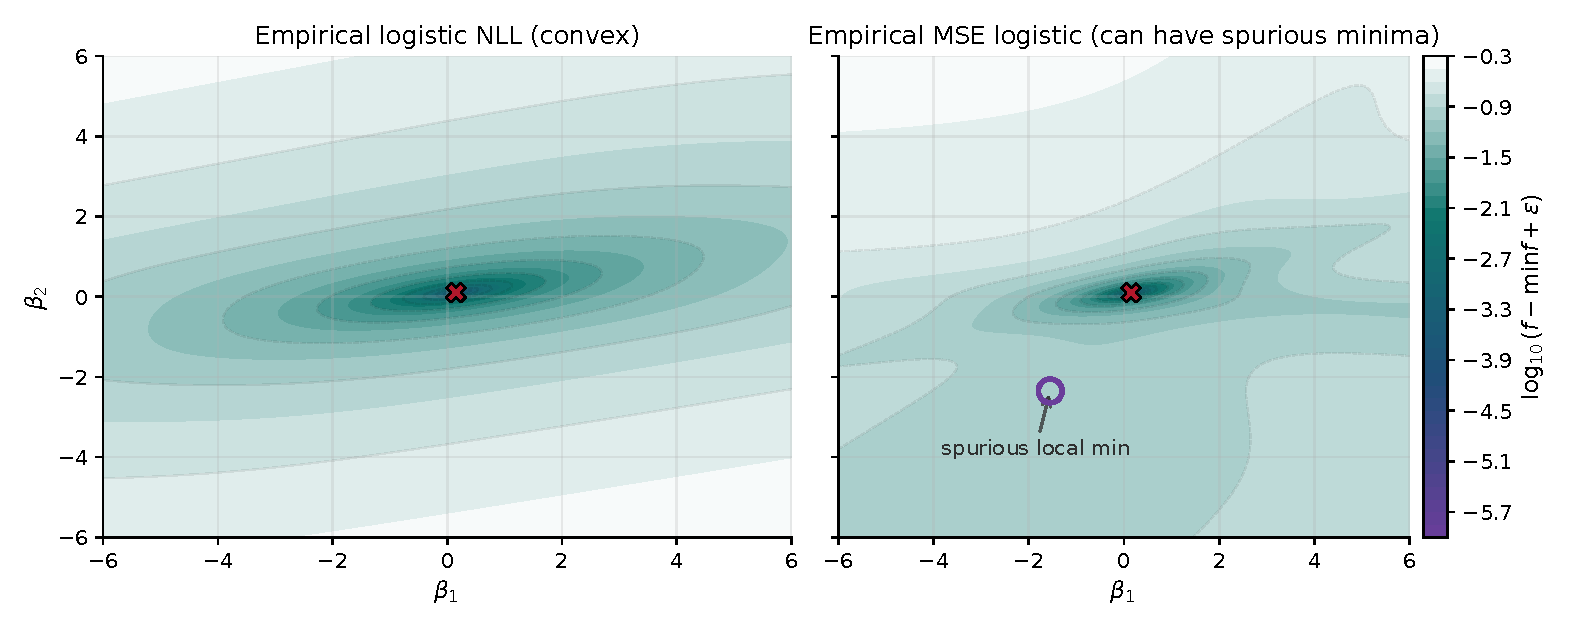
\includegraphics[width=\textwidth]{figures/handouts/convexity_optimization/fig_logistic_empirical_spurious}
  \caption{Empirical logistic landscapes on the dataset in \Cref{ex:logistic-empirical-spurious}.
  The plots show $\log_{10}(f-\min f+\varepsilon)$ for each objective.
  The red X marks the global minimizer in each panel.
  Left: the NLL is convex (one basin).
  Right: the squared-loss objective can have a spurious local minimum (circled), so a local method can get stuck.}
  \label{fig:logistic-empirical-spurious}
\end{figure}

\begin{figure}[t]
  \centering
  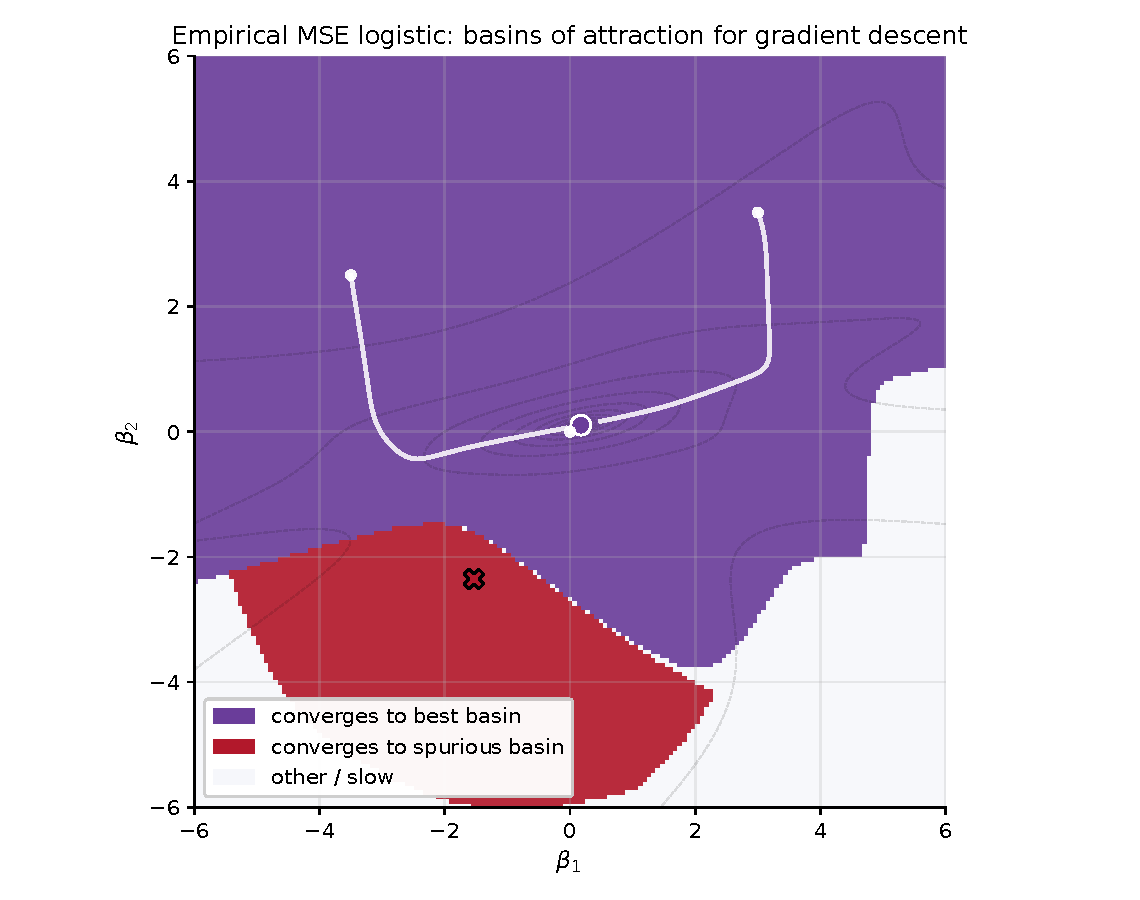
\includegraphics[width=0.92\textwidth]{figures/handouts/convexity_optimization/fig_logistic_empirical_basins}
  \caption{Basins of attraction for gradient descent on the empirical MSE-logistic objective in \Cref{ex:logistic-empirical-spurious}.
  The purple dot and red X mark the two local minimizers.
  Each initialization is colored by which local minimizer fixed-step GD (with $\eta=0.6$) converges to, and the overlaid paths show a few representative trajectories.}
  \label{fig:logistic-empirical-basins}
\end{figure}

Now assume a realizable population model:
\[
Y\mid X=x \sim \mathrm{Bernoulli}(p^\star(x)),
\qquad
p^\star(x) = \sigma(x^\top\beta^\star).
\]
Then the expected squared loss decomposes as
\[
\E\big[(Y-\sigma(X^\top\beta))^2\mid X\big]
= p^\star(X)(1-p^\star(X)) + \big(p^\star(X)-\sigma(X^\top\beta)\big)^2,
\]
so (up to an additive constant) the population objective becomes
\begin{equation}
R(\beta) = \E\big[(\sigma(X^\top\beta)-\sigma(X^\top\beta^\star))^2\big].
\label{eq:logistic-pop-risk}
\end{equation}

\begin{proposition}[One-point monotonicity in the realizable population squared-loss risk]
\label{prop:logistic-pop-one-point}
Assume $\E[\norm{X}_2]<\infty$, and let $R$ be as in \eqref{eq:logistic-pop-risk}. Then for all $\beta$,
\begin{equation}
\ip{\nabla R(\beta)}{\beta-\beta^\star} \ge 0.
\label{eq:one-point}
\end{equation}
In particular, along any ray $\beta(t)=\beta^\star+t(\beta-\beta^\star)$, the function $t\mapsto R(\beta(t))$ is nondecreasing for $t\ge 0$.
\end{proposition}

The next exercise isolates the population monotonicity calculation; structurally it plays the same role as the first-order convexity arguments in the Optimization unit.
\begin{exercise}[One-point monotonicity for realizable MSE-logistic]
\label{ex:logistic-one-point}
Prove \Cref{prop:logistic-pop-one-point}.
Let $\eta=X^\top\beta$ and $\eta^\star=X^\top\beta^\star$.
\begin{enumerate}[leftmargin=*]
  \item Differentiate under the expectation in \eqref{eq:logistic-pop-risk} to show that
  \[
  \nabla R(\beta)
  =2\,\E\Big[(\sigma(\eta)-\sigma(\eta^\star))\,\sigma'(\eta)\,X\Big].
  \]
  \item Show that
  \[
  \ip{\nabla R(\beta)}{\beta-\beta^\star}
  =2\,\E\Big[\sigma'(\eta)\,(\sigma(\eta)-\sigma(\eta^\star))(\eta-\eta^\star)\Big],
  \]
  and conclude it is nonnegative using only that $\sigma$ is increasing and $\sigma'\ge 0$.
  \item Deduce the ray-monotonicity statement by differentiating $g(t)=R(\beta^\star+t(\beta-\beta^\star))$.
\end{enumerate}
\end{exercise}

\SolutionBox[14]{%
\emph{Part (1).}
Differentiate \eqref{eq:logistic-pop-risk} under the expectation:
\[
R(\beta)=\E\big[(\sigma(X^\top\beta)-\sigma(X^\top\beta^\star))^2\big].
\]
Using the chain rule, $\nabla_\beta\sigma(X^\top\beta)=\sigma'(X^\top\beta)\,X$, hence
\[
\nabla R(\beta)
=2\,\E\Big[(\sigma(\eta)-\sigma(\eta^\star))\,\sigma'(\eta)\,X\Big],
\qquad
\eta=X^\top\beta,\ \eta^\star=X^\top\beta^\star.
\]

\emph{Part (2).}
Take the inner product with $(\beta-\beta^\star)$ and use $\ip{X}{\beta-\beta^\star}=\eta-\eta^\star$:
\[
\ip{\nabla R(\beta)}{\beta-\beta^\star}
=2\,\E\Big[\sigma'(\eta)\,(\sigma(\eta)-\sigma(\eta^\star))(\eta-\eta^\star)\Big].
\]
Since $\sigma'(\eta)\ge 0$ and $\sigma$ is increasing, we have
$(\sigma(\eta)-\sigma(\eta^\star))(\eta-\eta^\star)\ge 0$ pointwise.
Therefore the integrand is pointwise nonnegative, and the expectation is nonnegative as claimed.

\emph{Part (3) (ray monotonicity).}
For the ray $\beta(t)=\beta^\star+t(\beta-\beta^\star)$, define $g(t)=R(\beta(t))$.
By the chain rule,
\[
g'(t)=\ip{\nabla R(\beta(t))}{\beta-\beta^\star}\ge 0,
\]
so $t\mapsto R(\beta(t))$ is nondecreasing for $t\ge 0$.
(The argument uses only that the link is increasing with nonnegative derivative, so it holds for any such link function.)%
}

\begin{corollary}[Realizable population MSE-logistic has no spurious local minima]
\label{cor:logistic-pop-no-spurious}
Under the assumptions of \Cref{prop:logistic-pop-one-point}, every local minimizer of the realizable population risk $R$ in \eqref{eq:logistic-pop-risk} is global.
If in addition $\E[XX^\top]\succ 0$, then the unique global minimizer is $\beta^\star$.
\end{corollary}

\begin{exercise}[Stationarity + one-point monotonicity $\Rightarrow$ no spurious local minima]
\label{ex:logistic-one-point-no-spurious}
Prove \Cref{cor:logistic-pop-no-spurious} from \Cref{prop:logistic-pop-one-point}.
\begin{enumerate}[leftmargin=*]
  \item Let $\bar\beta$ be a local minimizer. Since $R$ is differentiable, $\nabla R(\bar\beta)=0$.
  Combine this with \Cref{eq:one-point} to show that
  \[
    0
    = \ip{\nabla R(\bar\beta)}{\bar\beta-\beta^\star}
    = 2\,\E\Big[\sigma'(\bar\eta)\,(\sigma(\bar\eta)-\sigma(\eta^\star))(\bar\eta-\eta^\star)\Big],
  \]
  where $\bar\eta=X^\top\bar\beta$ and $\eta^\star=X^\top\beta^\star$.
  Conclude that $\sigma(X^\top\bar\beta)=\sigma(X^\top\beta^\star)$ almost surely.
  \item Deduce that $R(\bar\beta)=0$, so $\bar\beta$ is a global minimizer.
  \item For uniqueness: show that if $R(\beta)=0$, then $X^\top(\beta-\beta^\star)=0$ almost surely, and deduce $\beta=\beta^\star$ under $\E[XX^\top]\succ 0$.
\end{enumerate}
\end{exercise}

\SolutionBox[14]{%
\emph{Part (1).}
Let $\bar\beta$ be a local minimizer of the differentiable function $R$.
Then $\nabla R(\bar\beta)=0$.
Applying \Cref{prop:logistic-pop-one-point} at $\beta=\bar\beta$ gives
\[
0
= \ip{\nabla R(\bar\beta)}{\bar\beta-\beta^\star}
= 2\,\E\Big[\sigma'(\bar\eta)\,(\sigma(\bar\eta)-\sigma(\eta^\star))(\bar\eta-\eta^\star)\Big],
\qquad \bar\eta=X^\top\bar\beta,\ \eta^\star=X^\top\beta^\star.
\]
The integrand is pointwise nonnegative because $\sigma'(\bar\eta)\ge 0$ and $\sigma$ is increasing, so the expectation can vanish only if the integrand is zero almost surely.
Since $\sigma'(z)>0$ for every finite $z$, this implies
\[
(\sigma(\bar\eta)-\sigma(\eta^\star))(\bar\eta-\eta^\star)=0
\qquad\text{almost surely.}
\]
Because $\sigma$ is strictly increasing, the product above is zero if and only if $\bar\eta=\eta^\star$, equivalently $\sigma(X^\top\bar\beta)=\sigma(X^\top\beta^\star)$ almost surely.

\emph{Part (2).}
If $\sigma(X^\top\bar\beta)=\sigma(X^\top\beta^\star)$ almost surely, then the integrand in \eqref{eq:logistic-pop-risk} vanishes almost surely, so
\[
R(\bar\beta)=\E\big[(\sigma(X^\top\bar\beta)-\sigma(X^\top\beta^\star))^2\big]=0.
\]
Since $R(\beta^\star)=0$ as well, $\bar\beta$ is a global minimizer.

\emph{Part (3) (uniqueness).}
If $R(\beta)=0$, then
\[
\E\big[(\sigma(X^\top\beta)-\sigma(X^\top\beta^\star))^2\big]=0,
\]
so $\sigma(X^\top\beta)=\sigma(X^\top\beta^\star)$ almost surely.
Since $\sigma$ is strictly increasing, this implies $X^\top(\beta-\beta^\star)=0$ almost surely.
Taking expectations yields
$(\beta-\beta^\star)^\top\E[XX^\top](\beta-\beta^\star)=0$.
If $\E[XX^\top]\succ 0$, then the quadratic form is strictly positive unless $\beta=\beta^\star$, so $\beta^\star$ is the unique global minimizer.%
}

The population MSE-logistic risk is nonconvex, but it still has the simple geometry that moving away from $\beta^\star$ does not help along any ray from $\beta^\star$.
This is qualitatively different from objectives like ecological logistic regression (\Cref{sec:ecological-logistic}), where aggregation introduces intrinsic nonconvexity and the landscape can have many distinct basins even under a clean population model.

Even with this benign global geometry, gradient descent can be slow because of saturation and flat plateaus.
The one-point monotonicity in \Cref{prop:logistic-pop-one-point} is a global geometry guarantee, but it is not a rate guarantee.
Far from $\beta^\star$, the squared-loss logistic objective can become very flat because the logistic link saturates:
$\sigma(z)\to 0$ or $1$ and $\sigma'(z)\to 0$ as $|z|\to\infty$.
The squared-loss gradient carries a factor of $\sigma'(X^\top\beta)$, so when the model is very confident (large $|X^\top\beta|$), the gradient can be tiny even if the objective value is not close to its minimum.
This mirrors the ``confidence weights'' story for convex NLL objectives:
in logistic NLL, curvature is largest near the decision boundary, while very confident points contribute little.
For squared loss, that same saturation suppresses the \emph{descent signal} itself, producing plateaus where $\norm{\nabla R(\beta)}_2$ is small even though $R(\beta)-R(\beta^\star)$ is not.

\begin{proposition}[Realizable squared-loss logistic: arbitrarily flat far from $\beta^\star$]
\label{prop:logistic-pop-flat}
Assume $\E[\norm{X}_2]<\infty$ and let $R$ be the realizable population risk \eqref{eq:logistic-pop-risk}.
Define $g(t)=R(t\beta^\star)$ for $t\ge 1$.
Then:
\begin{enumerate}[leftmargin=*]
  \item $g$ is nondecreasing on $[1,\infty)$ and converges to a finite limit $g(\infty)$.
  \item $\lim_{t\to\infty} g'(t)=0$ and $\lim_{t\to\infty}\norm{\nabla R(t\beta^\star)}_2=0$.
  \item If $\Pr(X^\top\beta^\star\neq 0)>0$, then $g(\infty)>0$.
\end{enumerate}
In particular, there are directions along which the landscape becomes arbitrarily flat even though the excess risk stays bounded away from $0$.
\end{proposition}

\emph{Proof idea.} See Exercise~\ref{ex:logistic-plateau}.

\begin{exercise}[Prove the plateau]
\label{ex:logistic-plateau}
In the realizable population model, let $g(t)=R(t\beta^\star)$ for $t\ge 1$.
\begin{enumerate}[leftmargin=*]
  \item Show that
  \[
    g'(t)=2\,\E\big[(\sigma(t\eta^\star)-\sigma(\eta^\star))\,\sigma'(t\eta^\star)\,\eta^\star\big],
    \qquad \eta^\star=X^\top\beta^\star,
  \]
  and conclude that $g$ is nondecreasing (hence $g(t)\to g(\infty)$ since $0\le g(t)\le 1$).
  \item Show that $g'(t)\to 0$ and $\nabla R(t\beta^\star)\to 0$ as $t\to\infty$.
  Interpret this as: \emph{without} a PL/strong-convexity-type condition, small gradient does not imply near-optimality.
  \item Assume $\Pr(\eta^\star\neq 0)>0$.
  Show that $g(\infty)>0$.
\end{enumerate}
\end{exercise}

\SolutionBox[12]{%
Write $\eta^\star=X^\top\beta^\star$ so that $g(t)=\E[(\sigma(t\eta^\star)-\sigma(\eta^\star))^2]$.

\emph{Part (1).}
Differentiate under the expectation:
by the chain rule,
\[
\frac{d}{dt}\sigma(t\eta^\star)=\sigma'(t\eta^\star)\,\eta^\star,
\]
so
\[
g'(t)
=\E\Big[2(\sigma(t\eta^\star)-\sigma(\eta^\star))\cdot \sigma'(t\eta^\star)\,\eta^\star\Big]
=2\,\E\big[(\sigma(t\eta^\star)-\sigma(\eta^\star))\,\sigma'(t\eta^\star)\,\eta^\star\big].
\]
For $t\ge 1$, $\sigma(t\eta^\star)-\sigma(\eta^\star)$ has the same sign as $(t-1)\eta^\star$ since $\sigma$ is increasing.
Because $\sigma'\ge 0$, the integrand is pointwise nonnegative, hence $g'(t)\ge 0$ and $g$ is nondecreasing.
Since $g(t)\in[0,1]$, it follows that $g(t)\to g(\infty)$ for some finite limit $g(\infty)$.

\emph{Part (2).}
For each fixed $\eta^\star\neq 0$, we have $t\eta^\star\to \pm\infty$ and therefore $\sigma'(t\eta^\star)\to 0$ as $t\to\infty$.
Also,
\[
\big|(\sigma(t\eta^\star)-\sigma(\eta^\star))\,\sigma'(t\eta^\star)\,\eta^\star\big|
\le \sigma'(0)\,|\eta^\star|
\le \sigma'(0)\,\norm{\beta^\star}_2\,\norm{X}_2,
\]
which is integrable since $\E[\norm{X}_2]<\infty$.
We will use the following standard fact: if random variables $Z_t$ satisfy $|Z_t|\le W$ with $\E[W]<\infty$ and $Z_t\to 0$ almost surely, then $\E[Z_t]\to 0$.
Applying this fact here gives $g'(t)\to 0$ as $t\to\infty$.

\smallskip
Similarly, differentiating \eqref{eq:logistic-pop-risk} gives
\[
\nabla R(t\beta^\star)
=2\,\E\big[(\sigma(t\eta^\star)-\sigma(\eta^\star))\,\sigma'(t\eta^\star)\,X\big].
\]
The integrand norm is bounded by $2\sigma'(0)\norm{X}_2$, and for each fixed $X$ the factor $\sigma'(t\eta^\star)$ tends to $0$ (or the bracketed term vanishes when $\eta^\star=0$), so the same reasoning lets us pass the limit through the expectation and conclude $\nabla R(t\beta^\star)\to 0$.

\emph{Part (3).}
As $t\to\infty$ we have $\sigma(t\eta^\star)\to 1$ when $\eta^\star>0$, $\sigma(t\eta^\star)\to 0$ when $\eta^\star<0$, and $\sigma(t\eta^\star)=\sigma(\eta^\star)=1/2$ when $\eta^\star=0$.
Since $0\le (\sigma(t\eta^\star)-\sigma(\eta^\star))^2\le 1$, we can apply the same fact (with $W=1$) to pass the limit through the expectation and obtain
\[
g(\infty)=\E\Big[(1-\sigma(\eta^\star))^2\mathbf{1}\{\eta^\star>0\} + \sigma(\eta^\star)^2\mathbf{1}\{\eta^\star<0\}\Big].
\]
If $\Pr(\eta^\star\neq 0)>0$, then the integrand is strictly positive on $\{\eta^\star\neq 0\}$, so $g(\infty)>0$.

Along this ray, the risk can remain bounded away from $0$ while the gradient (and directional derivative) goes to $0$.
Without a condition like PL/strong convexity, a small gradient does not by itself certify near-optimality.
}

Conditions like strong convexity or the PL inequality (\Cref{def:pl-inequality}) prevent this phenomenon: they rule out large flat regions away from the optimum by relating gradient size to suboptimality.
\Cref{prop:logistic-pop-flat} shows the realizable squared-loss logistic risk does not have such a global guarantee in general.

In the realizable population model, the one-point monotonicity in \Cref{prop:logistic-pop-one-point} is a \emph{global} geometric statement.
To get an actual rate for gradient descent, we also need a \emph{local curvature} condition near $\beta^\star$.
One simple sufficient condition is bounded features, which implies local strong convexity (hence a linear rate) around the optimum.

\begin{proposition}[Local linear convergence of gradient descent near $\beta^\star$]
\label{prop:logistic-pop-local-rate}
Assume $\E[XX^\top]\succeq \lambda I_d$ and $\norm{X}_2\le R$ almost surely for some $\lambda,R>0$.
Then at $\beta^\star$,
\[
\Hess R(\beta^\star)\succeq m_0 I_d,
\qquad
m_0 = 2\,\sigma'(R\norm{\beta^\star}_2)^2\,\lambda,
\]
and there exist $r>0$ and constants $0<m\le L<\infty$ such that the population risk $R$ in \eqref{eq:logistic-pop-risk} is $m$-strongly convex and $L$-smooth on the ball $\{\beta:\ \norm{\beta-\beta^\star}_2\le r\}$.
Consequently, gradient descent with step size $1/L$ initialized in this ball satisfies
\[
R(\beta^{(k)})-R(\beta^\star)
\le \left(1-\frac{m}{L}\right)^k\bigl(R(\beta^{(0)})-R(\beta^\star)\bigr)
\qquad\text{(see \citealp[\S9.3]{boyd_vandenberghe_2004_convex}).}
\]
\end{proposition}

\begin{proof}
Differentiate \eqref{eq:logistic-pop-risk} twice.
At $\beta=\beta^\star$, the cross term vanishes and the Hessian simplifies to
\[
\Hess R(\beta^\star)=2\,\E\big[\sigma'(X^\top\beta^\star)^2\,XX^\top\big].
\]
Since $\norm{X^\top\beta^\star}\le \norm{X}_2\norm{\beta^\star}_2\le R\norm{\beta^\star}_2$ almost surely, we have
$\sigma'(X^\top\beta^\star)\ge \sigma'(R\norm{\beta^\star}_2)>0$ almost surely (since $\sigma'$ is even and decreases with $|z|$), hence
\[
\Hess R(\beta^\star)\succeq 2\,\sigma'(R\norm{\beta^\star}_2)^2\,\E[XX^\top]\succeq 2\,\sigma'(R\norm{\beta^\star}_2)^2\,\lambda I_d.
\]
This is the claimed bound with $m_0=2\,\sigma'(R\norm{\beta^\star}_2)^2\,\lambda$.
Because $R$ is twice continuously differentiable and $\norm{X}_2\le R$ almost surely, $\Hess R(\beta)$ varies continuously in $\beta$ and is bounded on compact sets.
Therefore, on a sufficiently small ball around $\beta^\star$, the Hessian is bounded below by (say) $\tfrac12 m_0 I_d$ and above by $L I_d$ for some finite $L$, which gives local strong convexity and smoothness.
The linear convergence rate for gradient descent on an $m$-strongly convex and $L$-smooth function is standard (cited above).
\end{proof}

Under misspecification, hard multimodality can return.
If $p^\star(x)$ is not representable as $\sigma(x^\top\beta)$ (e.g.\ marginalizing over latent classes can yield mixtures of logits), then \eqref{eq:one-point} need not hold, and the population squared-loss risk can become bimodal with spurious local minima.
Benign global geometry often hinges on model and data assumptions.
This is one reason MLE (convex NLL) is often more stable than squared-loss fitting in logistic-type binary regression models.

\begin{example}[Misspecification can create a spurious local minimum for squared-loss logistic regression]
\label{ex:logistic-misspecified-spurious}
Consider a 1D feature $X$ that takes values $\{-2,-1,1,2\}$ with equal probability, and parameterize $\beta=(\beta_0,\beta_1)$ so that $q_\beta(x)=\sigma(\beta_0+\beta_1 x)$.
Let the true conditional probabilities be
\[
p^\star(-2)=0.49,\quad p^\star(-1)=0.87,\quad p^\star(1)=0.92,\quad p^\star(2)=0.36.
\]
This $p^\star$ is not representable as $q_\beta$, since it is not monotone in $x$.

For the population squared-loss risk $R_{\mathrm{MSE}}(\beta)=\E[(q_\beta(X)-p^\star(X))^2]$, a direct evaluation shows two distinct basins:
numerically, evaluating $R_{\mathrm{MSE}}$ on a grid reveals a global minimizer and a spurious local minimizer.
See \Cref{fig:logistic-landscape-2d}.
\end{example}

\begin{figure}[t]
  \centering
  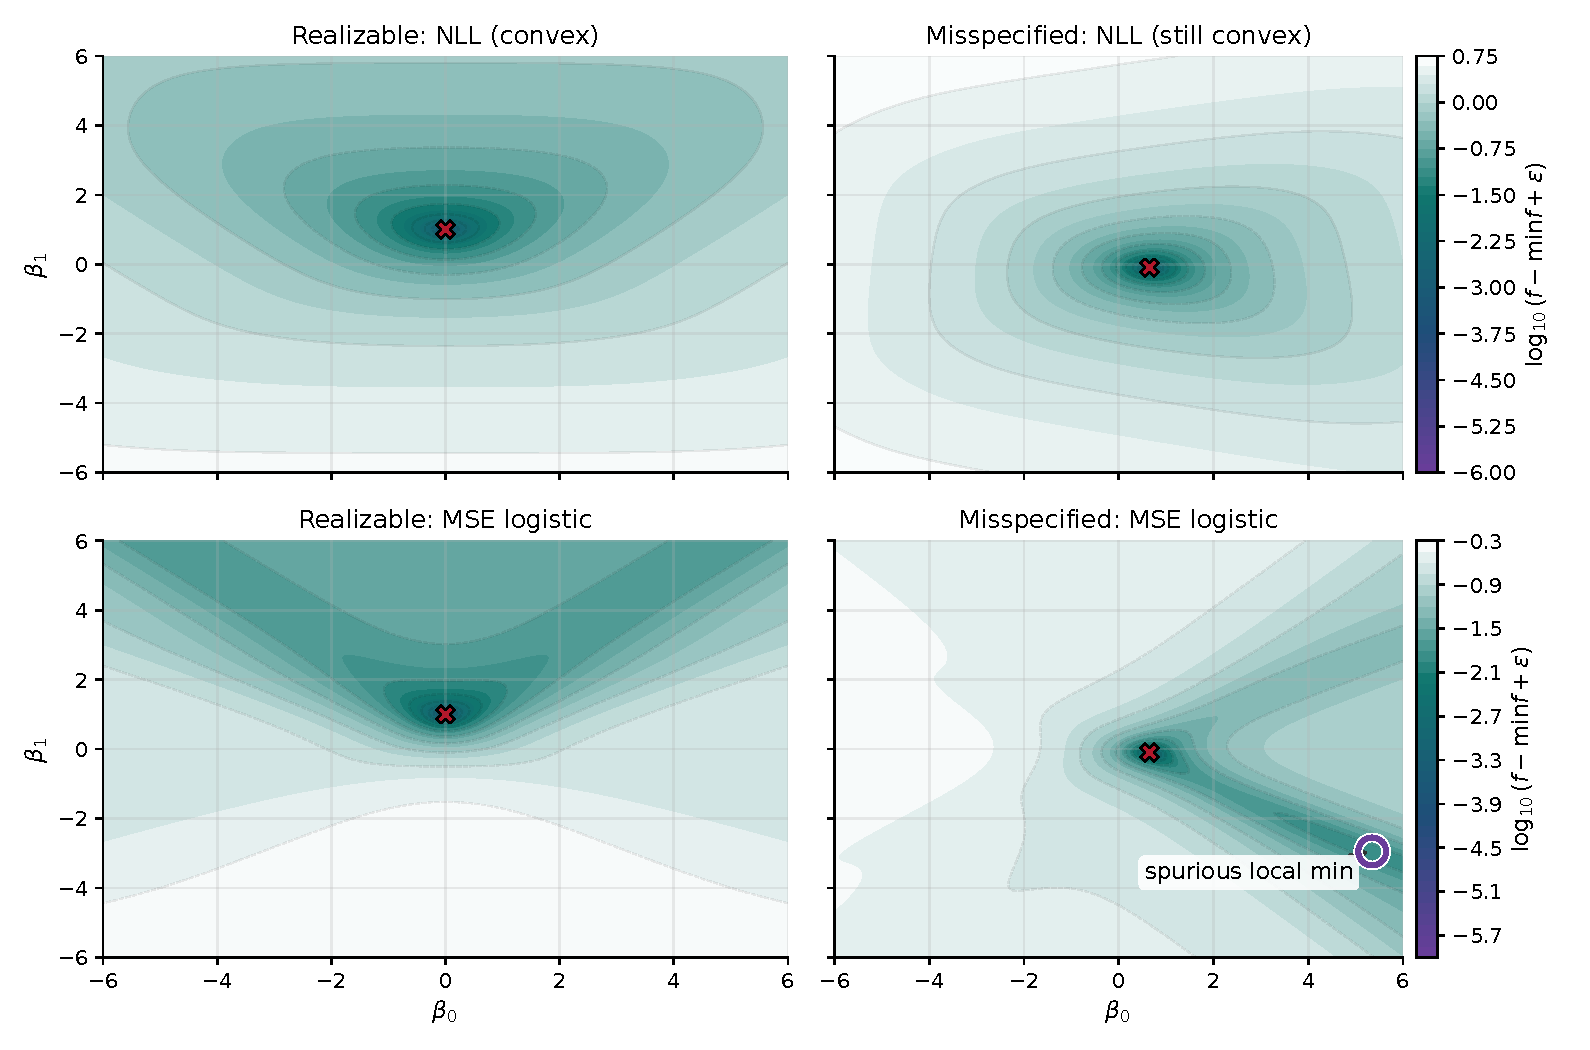
\includegraphics[width=\textwidth]{figures/handouts/convexity_optimization/fig_logistic_landscape_2d}
  \caption{A consistent contourf view of logistic landscapes in a 2D parameterization $\beta=(\beta_0,\beta_1)$.
  The plots show $\log_{10}(f-\min f+\varepsilon)$ for each objective, which makes basins comparable across panels.
  The red X marker indicates the global minimizer in each panel; in the bottom-right plot, the circled point is a spurious local minimum.
  In this example, the NLL landscape is unimodal in both realizable and misspecified settings, while the squared-loss landscape can develop extra basins under misspecification.}
  \label{fig:logistic-landscape-2d}
\end{figure}

% ------------------------------------------------------------
Example~I separates three distinct regimes.
Empirical MSE-logistic can create spurious basins; the realizable population risk has no spurious local minima but can still be slow because of broad plateaus; and misspecification can bring back genuinely wrong stable basins.
The response depends on the regime: use a stable objective when possible, use damping or line search when curvature is unreliable, and use restarts or stronger initializations when multiple basins are present.

% ------------------------------------------------------------
\section[Example II (phase retrieval)]{Example II: multimodality from symmetry, but only global optima in phase retrieval}
\label{sec:phase-retrieval}

In coherent diffraction imaging, optics, and astronomy, sensors measure intensities and lose phase.
A canonical real model is \emph{phase retrieval}:
\[
y_i = (a_i^\top x^\star)^2,\qquad i=1,\dots,m,
\]
where $x^\star\in\R^d$ is the unknown signal and $a_i$ are known sensing vectors.
A standard nonconvex least-squares objective is
\begin{equation}
F(x)=\frac{1}{4m}\sum_{i=1}^m\big((a_i^\top x)^2 - y_i\big)^2.
\label{eq:phase-empirical}
\end{equation}
This objective is nonconvex for structural reasons (it involves squares of linear forms),
and it is \emph{inherently} multimodal because $x^\star$ and $-x^\star$ generate the same data.

Like squared-loss logistic regression, phase retrieval is a smooth, nonconvex least-squares objective.
But here the nonconvexity is driven primarily by a \emph{symmetry}: $x^\star$ and $-x^\star$ generate the same data.
In population (for Gaussian designs), this symmetry produces multiple global optima but \emph{no} suboptimal local minima; the remaining stationary points are saddles.
This is ``benign'' nonconvexity (a strict-saddle picture), and it contrasts with ecological logistic regression (\Cref{sec:ecological-logistic}), where aggregation creates intrinsic nonconvexity and can lead to many distinct basins.
This ``benign geometry'' picture (multiple equivalent global minimizers; strict saddles elsewhere) appears broadly in modern tractable nonconvex problems; see \citet[\S2]{sun_qu_wright_2015_nonconvex_not_scary} and \citet[\S1]{zhang_qu_wright_2020_symmetry_geometry}.

\begin{figure}[t]
  \centering
  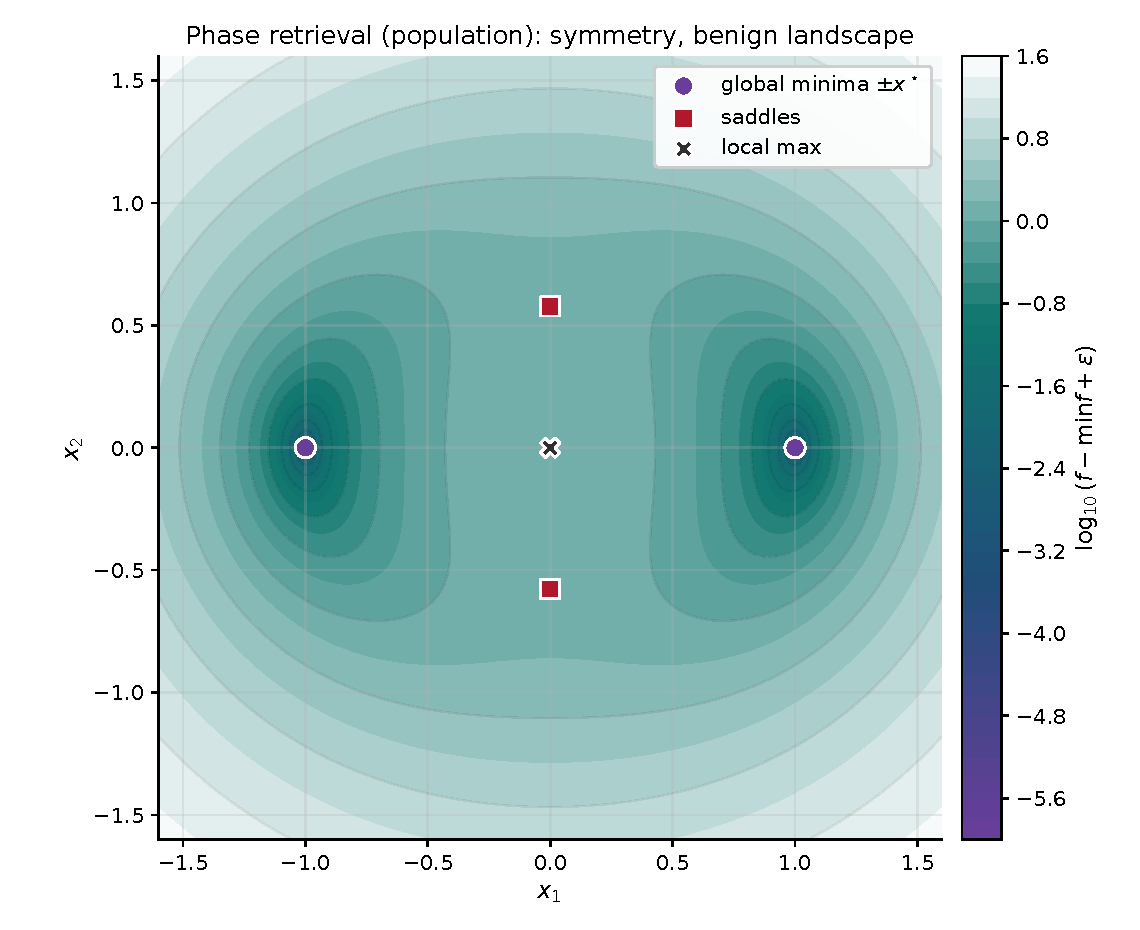
\includegraphics[width=0.86\textwidth]{figures/handouts/convexity_optimization/fig_phase_retrieval_landscape}
  \caption{Population phase retrieval in $d=2$: the landscape is nonconvex and symmetric ($x\sim -x$), but the only local minima are the two global minima $\pm x^\star$; other critical points are saddles or a local maximum at the origin.}
  \label{fig:phase-retrieval-landscape}
\end{figure}

For a clean population model, assume $a\sim N(0,I_d)$ and consider the \emph{population} objective
\begin{equation}
  f(x)=\frac12\,\E\Big[\big((a^\top x)^2 - (a^\top x^\star)^2\big)^2\Big].
  \label{eq:phase-pop}
\end{equation}

\begin{proposition}[Population phase retrieval: nonconvex but no spurious local minima]
\label{prop:phase-retrieval-benign}
For $f$ in \eqref{eq:phase-pop},
\begin{equation}
  f(x)
  =\frac{3}{2}\norm{x}^4 - \norm{x}^2\norm{x^\star}^2 - 2\ip{x}{x^\star}^2 + \frac{3}{2}\norm{x^\star}^4,
  \label{eq:phase-pop-closed-form}
\end{equation}
and the stationary points are:
\begin{enumerate}[leftmargin=*]
  \item global minima $x=\pm x^\star$ (value $0$),
  \item a local maximum at $x=0$,
  \item a saddle set $\{x:\ x\perp x^\star,\ \norm{x}=\norm{x^\star}/\sqrt{3}\}$.
\end{enumerate}
In particular, every local minimum is global.
\end{proposition}

\begin{exercise}[Phase retrieval: derive and classify the population stationary points]
\label{ex:phase-pop-derivation}
Prove \Cref{prop:phase-retrieval-benign}.
\begin{enumerate}[leftmargin=*]
  \item Expand \eqref{eq:phase-pop} and use the Gaussian fourth-moment identities
  \[
  \E[(a^\top u)^4]=3\norm{u}^4,
  \qquad
  \E[(a^\top u)^2(a^\top v)^2]=\norm{u}^2\norm{v}^2 + 2\ip{u}{v}^2,
  \]
  to obtain \eqref{eq:phase-pop-closed-form}.
  \item Differentiate \eqref{eq:phase-pop-closed-form} to get an explicit formula for $\nabla f(x)$.
  \item Solve $\nabla f(x)=0$ by decomposing $x=\alpha x^\star + u$ with $u\perp x^\star$.
  \item Classify the stationary points as global minima, a local maximum, and a saddle set.
\end{enumerate}
\end{exercise}

\SolutionBox[22]{%
\emph{Part (1) (closed form).}
Expanding the square in \eqref{eq:phase-pop} gives
\[
f(x)
=\frac12\,\E\big[(a^\top x)^4\big]
\;-\;\E\big[(a^\top x)^2(a^\top x^\star)^2\big]
\;+\;\frac12\,\E\big[(a^\top x^\star)^4\big].
\]
Apply the stated Gaussian fourth-moment identities with $u=x$ and $v=x^\star$ to get
\[
\E[(a^\top x)^4]=3\norm{x}^4,\qquad
\E[(a^\top x^\star)^4]=3\norm{x^\star}^4,
\]
and
\[
\E[(a^\top x)^2(a^\top x^\star)^2]=\norm{x}^2\norm{x^\star}^2 + 2\ip{x}{x^\star}^2.
\]
Substituting yields \eqref{eq:phase-pop-closed-form}.

\emph{Part (2) (gradient).}
Differentiate \eqref{eq:phase-pop-closed-form}:
\[
\nabla f(x)
= 6\norm{x}^2 x - 2\norm{x^\star}^2 x - 4\ip{x}{x^\star}x^\star
= (6\norm{x}^2-2\norm{x^\star}^2)x - 4\ip{x}{x^\star}x^\star.
\]

\emph{Part (3) (stationary points).}
Let $r=\norm{x^\star}_2$ and decompose $x=\alpha x^\star + u$ with $u\perp x^\star$.
Then $\ip{x}{x^\star}=\alpha r^2$ and $\norm{x}^2=\alpha^2r^2+\norm{u}^2$.
Setting $\nabla f(x)=0$ and matching the $u$ and $x^\star$ components gives
\[
(6\norm{x}^2-2r^2)\,u=0,
\qquad
\alpha\,(6\norm{x}^2-6r^2)=0.
\]
If $u=0$, then either $\alpha=0$ (so $x=0$) or $\norm{x}^2=r^2$ (so $\alpha=\pm 1$ and $x=\pm x^\star$).
If $u\neq 0$, then the first equation forces $\norm{x}^2=r^2/3$, and the second forces $\alpha=0$, hence
$x\perp x^\star$ and $\norm{x}=r/\sqrt{3}$.
This gives exactly the stationary-point list in \Cref{prop:phase-retrieval-benign}.

\emph{Part (4) (classification).}
Since $f$ in \eqref{eq:phase-pop} is an expectation of a square, $f(x)\ge 0$ for all $x$.
Also $f(\pm x^\star)=0$, so $\pm x^\star$ are global minima.

For $x=0$, the expansion \eqref{eq:phase-pop-closed-form} shows
\[
f(0)-f(x)= r^2\norm{x}^2 + 2\ip{x}{x^\star}^2 - \frac{3}{2}\norm{x}^4,
\]
which is strictly positive for all sufficiently small $x\neq 0$ (the quadratic term dominates), so $x=0$ is a local maximum.

Finally, if $x\perp x^\star$ and $\norm{x}=r/\sqrt{3}$, then the univariate restriction $t\mapsto f(x+t x^\star)$ has negative second derivative at $t=0$, so there is a direction of negative curvature.
Hence these points are saddles, and every local minimum is global.%
}

This is symmetry-driven nonconvexity with a strict-saddle geometry:
every non-optimal stationary point has a direction of negative curvature.

Phase retrieval is typically approached via the two-stage template in \Cref{alg:two-stage-template}:
use a cheap global initializer, then run a local method.
In the Gaussian model, there is a clean way to build a provably good direction estimate from a simple moment identity.
Assume the noiseless Gaussian design model $a_i \stackrel{\mathrm{iid}}{\sim} N(0,I_d)$ with measurements $y_i=(a_i^\top x^\star)^2$.
Define the \emph{spectral matrix}
\[
  Y = \frac{1}{m}\sum_{i=1}^m y_i a_i a_i^\top.
\]
Also define the radius estimate
\[
  \hat r^2 = \frac{1}{m}\sum_{i=1}^m y_i,
\]
which satisfies $\E[\hat r^2]=\norm{x^\star}_2^2$.
If $\hat u$ is a unit-norm top eigenvector of $Y$, then the standard spectral initializer is $x^{(0)}=\hat r\,\hat u$.

The next proposition explains why this initialization is reasonable.
It shows that (i) the population matrix $\E[Y]$ has a unique leading eigenvector in the $x^\star$ direction, and (ii) if the empirical $Y$ is close to $\E[Y]$ in operator norm then its leading eigenvector must be close to $\pm x^\star/\norm{x^\star}_2$.
(Here $\norm{M}_{\mathrm{op}}$ denotes the operator norm, i.e.\ the largest absolute eigenvalue for a symmetric matrix $M$.)

\begin{proposition}[Gaussian phase retrieval: why the spectral initializer points at $x^\star$]
\label{prop:phase-spectral-init}
Assume $x^\star\neq 0$, let $a\sim N(0,I_d)$, and set $y=(a^\top x^\star)^2$.
Write $r=\norm{x^\star}_2$ and $u^\star=x^\star/r$.
Define the population matrix
\[
  Y_{\mathrm{pop}} = \E\big[y\,a a^\top\big]
  = \E\big[(a^\top x^\star)^2 a a^\top\big].
\]
Then
\[
  Y_{\mathrm{pop}}=r^2 I_d + 2x^\star(x^\star)^\top,
\]
so the unique leading eigenvector of $Y_{\mathrm{pop}}$ is $u^\star$.
Moreover, if $Y$ is any symmetric matrix satisfying
\[
\norm{Y-Y_{\mathrm{pop}}}_{\mathrm{op}} \le \varepsilon\, r^2
\qquad\text{for some }\varepsilon\in(0,1),
\]
then for every unit-norm leading eigenvector $\hat u$ of $Y$ there exists a sign $s\in\{\pm 1\}$ such that
$\norm{\hat u-su^\star}_2\le \sqrt{2\varepsilon}$.
\end{proposition}

\begin{exercise}[Phase retrieval: why spectral initialization points at $x^\star$]
\label{ex:phase-spectral-spike}
Prove \Cref{prop:phase-spectral-init}.
Conclude that if the empirical matrix $Y$ is close to $Y_{\mathrm{pop}}$ in operator norm, then its top eigenvector is close to $\pm u^\star$ and the spectral initializer $x^{(0)}=\hat r\,\hat u$ is close to $\pm x^\star$.
\emph{Hint:} to compute $Y_{\mathrm{pop}}$, you can either compute entries using the Gaussian fourth-moment identity
$\E[a_i a_j a_k a_\ell]=\delta_{ij}\delta_{k\ell}+\delta_{ik}\delta_{j\ell}+\delta_{i\ell}\delta_{jk}$,
or compute the entries directly by expanding.
For the perturbation bound, compare quadratic forms $v^\top Y v$ and use $|v^\top (Y-Y_{\mathrm{pop}}) v|\le \norm{Y-Y_{\mathrm{pop}}}_{\mathrm{op}}$ for unit $v$.
Finally, explain in a sentence why one expects $\norm{Y-Y_{\mathrm{pop}}}_{\mathrm{op}}$ to be small when $m$ is large in the Gaussian model.
\end{exercise}

\SolutionBox[20]{%
Write $u=x^\star$ and expand $y=(a^\top u)^2=\sum_{k,\ell} u_k u_\ell a_k a_\ell$.
For each entry $(i,j)$,
\[
\E\!\big[y\,a_i a_j\big]
=\sum_{k,\ell} u_k u_\ell\,\E[a_i a_j a_k a_\ell]
=\sum_{k,\ell} u_k u_\ell\bigl(\delta_{ij}\delta_{k\ell}+\delta_{ik}\delta_{j\ell}+\delta_{i\ell}\delta_{jk}\bigr).
\]
The first term gives $\delta_{ij}\sum_k u_k^2=\delta_{ij}\norm{u}_2^2$.
The second and third terms each give $u_i u_j$.
Thus $\E[y\,a_i a_j]=\norm{u}_2^2\,\delta_{ij}+2u_i u_j$, i.e.
$Y_{\mathrm{pop}}=\norm{u}_2^2 I_d + 2uu^\top$.

For eigenvalues, note that $Y_{\mathrm{pop}}u=(\norm{u}_2^2+2\norm{u}_2^2)u=3\norm{u}_2^2 u$.
If $w\perp u$, then $uu^\top w=0$ so $Y_{\mathrm{pop}}w=\norm{u}_2^2 w$.
Hence the unique top eigenspace is $\mathrm{span}\{u\}$.

Let $r=\norm{u}_2$ and $u^\star=u/r$.
Let $\hat u$ be a unit top eigenvector of $Y$.
Write $E=Y-Y_{\mathrm{pop}}$ and assume $\norm{E}_{\mathrm{op}}\le \varepsilon r^2$.
Then
\[
\hat u^\top Y_{\mathrm{pop}} \hat u
= \hat u^\top Y \hat u - \hat u^\top E \hat u
\ge \lambda_{\max}(Y) - \norm{E}_{\mathrm{op}}
\ge (u^\star)^\top Y u^\star - \norm{E}_{\mathrm{op}}
\ge 3r^2 - 2\varepsilon r^2.
\]
On the other hand,
$
\hat u^\top Y_{\mathrm{pop}} \hat u
= r^2 + 2r^2\,|\ip{\hat u}{u^\star}|^2.
$
Combining gives $|\ip{\hat u}{u^\star}|^2\ge 1-\varepsilon$.
Choosing the sign that maximizes the inner product,
\[
\min\{\norm{\hat u-u^\star}_2,\norm{\hat u+u^\star}_2\}^2
=2\bigl(1-|\ip{\hat u}{u^\star}|\bigr)
\le 2\bigl(1-|\ip{\hat u}{u^\star}|^2\bigr)
\le 2\varepsilon.
\]

The matrix $Y$ is an empirical average of i.i.d.\ symmetric matrices with mean $Y_{\mathrm{pop}}$.
To make this quantitative in high dimensions, one uses concentration inequalities for random matrices to bound $\norm{Y-Y_{\mathrm{pop}}}_{\mathrm{op}}$ with high probability; see \citet[\S2.2]{zhang_qu_wright_2020_symmetry_geometry} for discussion and references.
These probability tools are largely orthogonal to our focus here.%
}

Once you have an initialization that is close to $\pm x^\star$, the local stage behaves like the convex story again.
In the Gaussian population objective, $\pm x^\star$ are not only global minima: they are \emph{locally strongly convex} minima, so the standard local strong-convexity analysis from the Optimization unit gives a linear rate while the iterates remain in that neighborhood.

\begin{exercise}[Phase retrieval: local convexity near $\pm x^\star$ in the population objective]
\label{ex:phase-pop-local-strong-convex}
For the population objective $f$ in \eqref{eq:phase-pop-closed-form}, compute the Hessian $\Hess f(x)$ and show that
\[
\Hess f(x^\star)=4\norm{x^\star}_2^2 I_d + 8x^\star(x^\star)^\top.
\]
Deduce the eigenvalues of $\Hess f(x^\star)$ and interpret this as a local condition-number statement near $x^\star$.
\end{exercise}

\SolutionBox[12]{%
Differentiate the gradient formula in the solution to \Cref{ex:phase-pop-derivation}:
for $x\in\R^d$,
\[
\Hess f(x)=12xx^\top + (6\norm{x}_2^2-2\norm{x^\star}_2^2)I_d - 4x^\star(x^\star)^\top.
\]
At $x=x^\star$ this becomes
\[
\Hess f(x^\star)=(12-4)x^\star(x^\star)^\top + 4\norm{x^\star}_2^2 I_d
=8x^\star(x^\star)^\top + 4\norm{x^\star}_2^2 I_d.
\]
Along $u^\star=x^\star/\norm{x^\star}_2$ the eigenvalue is $12\norm{x^\star}_2^2$, and along any direction orthogonal to $x^\star$ the eigenvalue is $4\norm{x^\star}_2^2$.
So near $x^\star$ the population objective is well conditioned (local condition number $3$), which is exactly the regime where local methods behave like in the convex case.%
}

These pieces give the standard Gaussian-model story:
spectral initialization supplies a direction close to $\pm x^\star$, and the local geometry near $\pm x^\star$ is strongly convex, so local methods converge quickly once initialized there.
Rigorous finite-sample analyses follow this template; see \citet[\S2.2]{zhang_qu_wright_2020_symmetry_geometry} and references therein.

Phase retrieval shows a different kind of nonconvexity.
The sign symmetry creates multiple optima, but they are equivalent, and the remaining stationary points are saddles rather than bad local minima.
The right response is therefore not exhaustive global search; it is a coarse initializer, such as a spectral method, followed by local refinement inside the basin of $\pm x^\star$.



% ------------------------------------------------------------
\section[Example III (ecological logistic)]{Example III: hard nonconvexity from aggregation in ecological logistic regression}
\label{sec:ecological-logistic}

In some applications we observe covariates at the unit level but only aggregated outcomes.
For example, we might see covariates $x_{g,1},\dots,x_{g,n_g}$ for individuals in a group (a precinct, a cohort, a batch),
but instead of observing the binary outcomes $Y_{g,i}\in\{0,1\}$ we only observe the group total
\[
Z_g = \sum_{i=1}^{n_g} Y_{g,i}.
\]
Many different binary vectors $(Y_{g,1},\dots,Y_{g,n_g})$ can produce the same total $Z_g$, so the likelihood for $\beta$ must marginalize over a large discrete set of latent ``assignments.''

Assume a logistic model at the unit level:
\[
\Pr(Y_{g,i}=1\mid x_{g,i},\beta)=\sigma(x_{g,i}^\top\beta),
\qquad i=1,\dots,n_g,
\]
with conditional independence across $i$ given the covariates.
Write $p_{g,i}(\beta)=\sigma(x_{g,i}^\top\beta)$.
Then $Z_g$ is a sum of independent but non-identically distributed Bernoulli random variables (a Poisson--binomial model), and the marginal likelihood contains $\binom{n_g}{z_g}$ terms.
The resulting negative log-likelihood is typically nonconvex in $\beta$.
This combinatorial marginalization also creates a separate difficulty that is easy to miss if we focus only on the geometry:
when $n_g$ is large, the likelihood term $\Pr(Z_g=z_g\mid x_{g,1},\dots,x_{g,n_g},\beta)$ can be expensive to evaluate repeatedly inside an optimizer.
The naive computation is literally a sum over $\binom{n_g}{z_g}$ assignments (as in \Cref{ex:eco-logistic-nonconvex}), which is intractable for large groups.
This ``optimization + marginalization'' pattern is common in latent-variable models: hard landscapes and expensive objective evaluations can come together.

An empirical negative log-likelihood objective for $G$ independent groups is
\begin{equation}
  f(\beta)
  =
  -\frac{1}{G}\sum_{g=1}^G \log \Pr(Z_g=z_g \mid x_{g,1},\dots,x_{g,n_g},\beta).
  \label{eq:eco-logistic-obj}
\end{equation}
Two edge cases are instructive.
In the special case where the covariates are constant within each group ($x_{g,i}\equiv x_g$), we have
$Z_g\sim \mathrm{Binomial}(n_g,\sigma(x_g^\top\beta))$, and \eqref{eq:eco-logistic-obj} reduces to the usual convex binomial logistic-regression objective from the Optimization unit.
At the other extreme, if $d=1$ with $\beta=(\beta_0,\beta_1)$ and each group contains covariates in $\pm$ pairs (for every $x$ the value $-x$ appears with the same multiplicity), then the marginal likelihood is symmetric in the slope: it is unchanged under $\beta_1\mapsto -\beta_1$.
This kind of symmetry reflects a genuine non-identifiability from totals alone.

\begin{exercise}[Ecological logistic regression: two easy special cases]
\label{ex:eco-logistic-edge-cases}
\begin{enumerate}[leftmargin=*]
  \item Suppose $x_{g,i}\equiv x_g$ within each group.
  Show that $Z_g\sim \mathrm{Binomial}(n_g,\sigma(x_g^\top\beta))$ and conclude that the corresponding negative log-likelihood is convex in $\beta$.
  \item Assume $d=1$ with $\beta=(\beta_0,\beta_1)$ and suppose the multiset $\{x_1,\dots,x_n\}$ is symmetric: for every $x$ it contains $-x$ with the same multiplicity.
  Show that, for every $z$,
  \[
    \Pr(Z=z\mid x_1,\dots,x_n,(\beta_0,\beta_1))
    =
    \Pr(Z=z\mid x_1,\dots,x_n,(\beta_0,-\beta_1)).
  \]
  Conclude that the likelihood for $\beta_1$ is an even function, so the sign of the slope is not identifiable from $Z$ alone in such a balanced design.
\end{enumerate}
\end{exercise}

\SolutionBox[14]{%
\emph{Part (1).}
If $x_{g,i}\equiv x_g$, then conditional on $x_g$ the unit-level outcomes are i.i.d.\ Bernoulli with success probability $\sigma(x_g^\top\beta)$.
Therefore $Z_g=\sum_{i=1}^{n_g}Y_{g,i}\sim \mathrm{Binomial}(n_g,\sigma(x_g^\top\beta))$.
Up to an additive constant (independent of $\beta$), the per-group negative log-likelihood can be written as a function of the scalar $\eta=x_g^\top\beta$:
\[
\ell_g(\beta)
= -z_g\,\eta + n_g\log(1+e^\eta).
\]
Since $\frac{d^2}{d\eta^2}\ell_g(\eta)=n_g\,\sigma'(\eta)\ge 0$, the map $\eta\mapsto \ell_g(\eta)$ is convex.
Composing a convex function with a linear map $\beta\mapsto x_g^\top\beta$ preserves convexity, so $\ell_g$ is convex in $\beta$.
Summing over $g$ preserves convexity, hence the full objective is convex.

\emph{Part (2).}
Write $p_i(\beta_0,\beta_1)=\sigma(\beta_0+\beta_1 x_i)$.
Replacing $\beta_1$ by $-\beta_1$ replaces $p_i$ by $\tilde p_i=\sigma(\beta_0-\beta_1 x_i)$.
By the assumed symmetry of the multiset $\{x_i\}$, the multiset $\{\tilde p_i\}$ is the same as $\{p_i\}$ up to a permutation (each $x$ is paired with $-x$).
But the distribution of $Z=\sum_i Y_i$ depends only on the multiset of success probabilities, not on how they are ordered, so $\Pr(Z=z\mid x_1,\dots,x_n,(\beta_0,\beta_1))=\Pr(Z=z\mid x_1,\dots,x_n,(\beta_0,-\beta_1))$ for every $z$.
Thus the likelihood is an even function of $\beta_1$, which means the sign of the slope is not identifiable from totals in this balanced design.%
}

This example ties directly to the empirical-versus-population theme from Example~I.
There the bad basins can be a finite-sample artifact under benign population geometry; here the nonconvexity is intrinsic, because even under the correct model and infinite data aggregation forces us to marginalize over discrete latent assignments.
That marginalization step is also the bridge to the Expectation--maximization subsection of the Augmented-state optimization unit: once the assignments are latent, the natural algorithmic object is the EM update map, which alternates exact conditional expectations with parameter updates, rather than a single closed-form convex objective.

To emphasize this, it is useful to look at a \emph{population} version of \eqref{eq:eco-logistic-obj}.
Let $X=(x_1,\dots,x_n)$ denote a random group of covariates and let $Z$ be generated from the model under a true parameter $\beta^\star$.
Define the population objective
\[
F(\beta)=\E\big[-\log \Pr(Z\mid X,\beta)\big].
\]
Because the model is correctly specified, $F$ is minimized at (an observationally equivalent version of) $\beta^\star$.
However, as \Cref{fig:eco-logistic-pop-landscape} illustrates, $F$ can still have multiple separated basins and spurious local minima.

\begin{figure}[H]
  \centering
  \begin{tikzpicture}
  \pgfplotsset{table/search path={figures/handouts/convexity_optimization/,../../figures/handouts/convexity_optimization/,Lecture Tex/figures/handouts/convexity_optimization/}}

  \begin{axis}[
    width=0.88\linewidth,
    height=6.6cm,
    view={0}{90},
    axis lines=left,
    xlabel={$\beta_0$},
    ylabel={$\beta_1$},
    tick style={stat221Gray},
    tick label style={font=\small},
    label style={font=\small},
    xmin=-1.0, xmax=3.5,
    ymin=-2.0, ymax=2.0,
    point meta min=-4,
    point meta max=0.75,
    colormap={stat221landscape}{
      color=(stat221Purple)
      color=(stat221Blue)
      color=(stat221Teal)
      color=(white)
    },
    colorbar,
    colorbar style={
      ylabel={$\log_{10}(F-\min F+\varepsilon)$},
      width=0.32cm,
      yticklabel style={font=\small},
      ylabel style={font=\small},
      tick style={stat221Gray},
    },
  ]
    \addplot3[
      surf,
      shader=interp,
      mesh/rows=81,
      draw=none,
    ]
    table [x=beta0, y=beta1, z=loggap] {data_ecological_logistic_population_landscape.dat};

    % True parameter beta^*.
    \addplot3[only marks,mark=x,mark size=4.2,very thick,color=white] coordinates {(0.3,1.2,0.75)};
    \addplot3[only marks,mark=x,mark size=3.6,very thick,color=stat221Red] coordinates {(0.3,1.2,0.75)};

    % A few spurious local minima (approximate locations; shown as open circles).
    \addplot3[only marks,mark=o,mark size=4.0,very thick,color=white,fill=none] coordinates {(2.2,-1.05,0.75) (2.5,-1.15,0.75) (2.7,-1.25,0.75)};
    \addplot3[only marks,mark=o,mark size=3.4,very thick,color=stat221Gray,fill=none] coordinates {(2.2,-1.05,0.75) (2.5,-1.15,0.75) (2.7,-1.25,0.75)};
  \end{axis}
\end{tikzpicture}

  \caption{A toy \emph{population} objective for ecological logistic regression in a 2D parameterization $\beta=(\beta_0,\beta_1)$.
  Each group has $n=6$ units and is equally likely to have covariates $(-4,-3,-2,2,3,4)$, $(-3,-1,1,2,3,4)$, or $(-2,-1,1,2,3,4)$ (in $d=1$); outcomes are generated under $\beta^\star=(0.3,1.2)$.
  The plot shows $\log_{10}(F-\min F+\varepsilon)$, as in \Cref{fig:logistic-landscape-2d}; the red X marks $\beta^\star$ and the open circles mark three spurious local minima in this toy example.}
  \label{fig:eco-logistic-pop-landscape}
\end{figure}

\begin{exercise}[Ecological logistic regression: marginalization and nonconvexity]
\label{ex:eco-logistic-nonconvex}
Fix one group with covariates $x_1,\dots,x_n\in\R^d$ and observe $Z=z$.
Let $p_i(\beta)=\sigma(x_i^\top\beta)$.
\begin{enumerate}[leftmargin=*]
  \item Show that
  \[
    \Pr(Z=z\mid x_1,\dots,x_n,\beta)
    =
    \sum_{\substack{S\subseteq\{1,\dots,n\}\\|S|=z}}
    \ \prod_{i\in S} p_i(\beta)\prod_{j\notin S}\bigl(1-p_j(\beta)\bigr).
  \]
  Interpret this as summing over all ways to choose which $z$ units are the successes.
  \item Specialize to $n=2$ and $z=1$ in $d=1$ with covariates $x_1=a$ and $x_2=b$.
  Let $\ell(\beta)$ be the negative log-likelihood $-\log \Pr(Z=1\mid a,b,\beta)$ with no regularization.
  Show that $\ell''(0)=\tfrac12 ab$.
  Conclude that $\ell$ is not convex whenever $ab<0$.
\end{enumerate}
\end{exercise}

\SolutionBox[20]{%
\emph{Part (1).}
Condition on the covariates.
For any binary vector $y=(y_1,\dots,y_n)\in\{0,1\}^n$, conditional independence gives
\[
\Pr(Y_1=y_1,\dots,Y_n=y_n\mid x_1,\dots,x_n,\beta)
=
\prod_{i=1}^n p_i(\beta)^{y_i}\bigl(1-p_i(\beta)\bigr)^{1-y_i}.
\]
The event $\{Z=z\}$ is the union of all assignments $y$ with exactly $z$ ones, so summing over those assignments yields
\[
\Pr(Z=z\mid x_1,\dots,x_n,\beta)
=
\sum_{\substack{y\in\{0,1\}^n\\ \sum_i y_i=z}}
\ \prod_{i=1}^n p_i(\beta)^{y_i}\bigl(1-p_i(\beta)\bigr)^{1-y_i}.
\]
Reindexing the sum by the subset $S=\{i:\ y_i=1\}$ (which has $|S|=z$) gives the stated formula.

\emph{Part (2).}
For $n=2$ and $z=1$, let $p_1(\beta)=\sigma(a\beta)$ and $p_2(\beta)=\sigma(b\beta)$.
Then
\[
q(\beta)=\Pr(Z=1\mid a,b,\beta)
 = p_1(1-p_2) + (1-p_1)p_2
 = p_1+p_2-2p_1p_2,
\]
and $\ell(\beta)=-\log q(\beta)$.
At $\beta=0$ we have $p_1=p_2=\tfrac12$, so $q(0)=\tfrac12$.
Also $p_1'(\beta)=a\,p_1(1-p_1)$ and $p_2'(\beta)=b\,p_2(1-p_2)$, so $p_1'(0)=a/4$ and $p_2'(0)=b/4$.
A direct differentiation gives $q'(0)=0$ and
\[
q''(0)=-4p_1'(0)p_2'(0)=-4\cdot\frac{a}{4}\cdot\frac{b}{4}=-\frac{ab}{4}.
\]
Since $\ell'=-q'/q$ and $q'(0)=0$, we have $\ell''(0)=-(q''(0)/q(0))$ and therefore
\[
\ell''(0)
=-\frac{q''(0)}{q(0)}
=-\frac{-ab/4}{1/2}
=\frac{ab}{2}.
\]
If $ab<0$, then $\ell''(0)<0$, so $\ell$ is not convex.
}

Even though the landscape can be globally hard (and even the population objective can have spurious basins, as in \Cref{fig:eco-logistic-pop-landscape}), there is still a familiar ``convex'' story \emph{locally} around the true parameter under correct specification.
When the model is locally identifiable, the population objective has a neighborhood of $\beta^\star$ on which it is convex (indeed strongly convex).
One convenient way to see this in ecological logistic regression is to expose the probabilistic structure behind the gradient and Hessian: the observed-data objective involves marginalizing over latent assignments, and its Hessian can be written as a difference of two covariance matrices.
After averaging over the random total $Z$ under the true model, that difference becomes a covariance by the law of total covariance.

\begin{exercise}[Ecological logistic regression: DC structure and local convexity near $\beta^\star$]
\label{ex:eco-logistic-pop-local-convex}
Fix covariates $x_1,\dots,x_n\in\R^d$.
For $\beta\in\R^d$, let $V_1,\dots,V_n$ be independent Bernoulli random variables with
\[
\Pr(V_j=1\mid x_j,\beta)=\sigma(x_j^\top\beta),
\qquad j=1,\dots,n,
\]
and define
\[
U = \sum_{j=1}^n x_j V_j,
\qquad
Z = \sum_{j=1}^n V_j.
\]
For an observed total $Z=z$, write $L_z(\beta)=-\log \Pr(Z=z\mid x_1,\dots,x_n,\beta)$.
\begin{enumerate}[leftmargin=*]
  \item Show the \emph{difference-of-convex (DC)} form
  \[
  L_z(\beta)
  =\sum_{j=1}^n \log\bigl(1+e^{x_j^\top\beta}\bigr)
  -\log\left(\sum_{\substack{S\subseteq\{1,\dots,n\}\\|S|=z}} \exp\Big(\sum_{j\in S} x_j^\top\beta\Big)\right).
  \]
  \item Show that $\nabla L_z(\beta)=\E[U]-\E[U\mid Z=z]$.
  \item Show that $\Hess L_z(\beta)=\mathrm{Cov}(U)-\mathrm{Cov}(U\mid Z=z)$.
  (Hint: for $g(\beta)=\log\sum_k e^{a_k^\top\beta}$, the Hessian is the covariance of the vectors $\{a_k\}$ under the corresponding softmax weights.)
  \item Consider the population objective $F(\beta)=\E[L_Z(\beta)]$ when $Z$ is generated under a true parameter $\beta^\star$.
  Assuming the outer expectation defining $F$ can be differentiated twice under the integral sign, use the conditional law of total covariance,
  \[
    \mathrm{Cov}(U\mid X)=\E[\mathrm{Cov}(U\mid Z,X)\mid X] + \mathrm{Cov}(\E[U\mid Z,X]\mid X),
  \]
  to show that
  \[
    \E\big[\Hess L_Z(\beta^\star)\mid X\big]
    = \mathrm{Cov}\big(\E[U\mid Z,X]\mid X\big)\succeq 0.
  \]
  Deduce that
  \[
    \Hess F(\beta^\star)
    = \E\Big[\mathrm{Cov}\big(\E[U\mid Z,X]\mid X\big)\Big]\succeq 0.
  \]
  Conclude that if $\Hess F(\beta^\star)\succ 0$, then $F$ is locally strongly convex on a neighborhood of $\beta^\star$.
\end{enumerate}
\end{exercise}

\SolutionBox[22]{%
\emph{Part (1).}
Write $\eta_j=x_j^\top\beta$ and $p_j=\sigma(\eta_j)=e^{\eta_j}/(1+e^{\eta_j})$.
For any subset $S$ with $|S|=z$,
\[
\Pr(V_j=1\ \forall j\in S,\ V_j=0\ \forall j\notin S\mid x_1,\dots,x_n,\beta)
=\prod_{j\in S}p_j\prod_{j\notin S}(1-p_j)
=\frac{\exp(\sum_{j\in S}\eta_j)}{\prod_{j=1}^n(1+e^{\eta_j})}.
\]
Summing over all $S$ with $|S|=z$ gives
\[
\Pr(Z=z\mid x_1,\dots,x_n,\beta)
=\frac{\sum_{|S|=z}\exp(\sum_{j\in S}\eta_j)}{\prod_{j=1}^n(1+e^{\eta_j})}.
\]
Taking $-\log$ yields the stated DC representation.

\emph{Parts (2) and (3).}
The first term in $L_z$ has gradient $\sum_j \sigma(\eta_j)x_j$ and Hessian $\sum_j \sigma'(\eta_j)x_jx_j^\top$.
Since $U=\sum_j x_j V_j$ with independent Bernoulli coordinates, these are exactly $\E[U]$ and $\mathrm{Cov}(U)$.

For the second term, define a probability distribution on subsets $S$ of size $z$ by
\[
w_S(\beta)\propto \exp\Big(\sum_{j\in S}x_j^\top\beta\Big),
\qquad |S|=z.
\]
This is the conditional law of the success set $\{j:\ V_j=1\}$ given $Z=z$ under parameter $\beta$.
Therefore
\[
\nabla \log\Big(\sum_{|S|=z} e^{\sum_{j\in S}x_j^\top\beta}\Big)
  = \sum_{|S|=z} w_S(\beta)\sum_{j\in S}x_j
  = \E[U\mid Z=z],
\]
and differentiating once more gives
\[
\Hess\!\left(\log\Big(\sum_{|S|=z} e^{\sum_{j\in S}x_j^\top\beta}\Big)\right)
=\mathrm{Cov}(U\mid Z=z),
\]
which yields $\nabla L_z=\E[U]-\E[U\mid Z=z]$ and $\Hess L_z=\mathrm{Cov}(U)-\mathrm{Cov}(U\mid Z=z)$.

\emph{Part (4).}
Now let $X=(x_1,\dots,x_n)$ be random, and assume we may differentiate the outer expectation in $F(\beta)=\E[L_Z(\beta)]$ twice under the integral sign.
Conditional on $X$ and at $\beta^\star$, take expectations over $Z$:
\[
\E\big[\Hess L_Z(\beta^\star)\mid X\big]
=\mathrm{Cov}(U\mid X)-\E[\mathrm{Cov}(U\mid Z,X)\mid X].
\]
By the conditional law of total covariance,
\[
\mathrm{Cov}(U\mid X)
=\E[\mathrm{Cov}(U\mid Z,X)\mid X] + \mathrm{Cov}(\E[U\mid Z,X]\mid X),
\]
so the difference is
\[
\E\big[\Hess L_Z(\beta^\star)\mid X\big]
=\mathrm{Cov}(\E[U\mid Z,X]\mid X)\succeq 0.
\]
Taking outer expectations gives
\[
\Hess F(\beta^\star)
=\E\big[\Hess L_Z(\beta^\star)\big]
=\E\Big[\mathrm{Cov}(\E[U\mid Z,X]\mid X)\Big]\succeq 0.
\]
If this unconditional Hessian is positive definite, then by continuity of $\Hess F$ there exists a radius $r>0$ such that $\Hess F(\beta)\succeq \tfrac12 \Hess F(\beta^\star)\succ 0$ on $\{\beta:\ \norm{\beta-\beta^\star}_2\le r\}$, which implies local strong convexity of $F$ on that neighborhood.%
}

This example still fits the two-stage template in \Cref{alg:two-stage-template}, but the coarse stage is less structured.
In practice, one often uses multiple random starts or a warm start from a crude convex surrogate, then runs a local optimizer with line search or damping on the true nonconvex objective \eqref{eq:eco-logistic-obj} and keeps the best solution found.

Ecological logistic regression is the genuinely hard case in this note.
Aggregation forces a sum over latent assignments, so the objective can have many distinct basins even under correct specification.
The practical response is usually robust search rather than a single clever local method: several starts, warm starts from crude convex surrogates when available, and then local refinement with damping or line search on the true objective.



% ------------------------------------------------------------
\section{Diagnosing nonconvex objectives}
\label{sec:checklist-streamlined}

``Nonconvex'' is not a single regime.
Squared-loss logistic regression is close to convex: the empirical objective can have spurious minima, yet under realizability the population geometry is benign and locally strongly convex near $\beta^\star$.
Phase retrieval is symmetry-driven: there can be multiple equivalent optima but no bad local minima.
Ecological logistic regression is intrinsically hard because aggregation induces latent assignments and the resulting marginal likelihood can have many distinct basins.
The right response depends on which regime you are in: stable objectives when available, spectral or other coarse initialization when symmetry is the issue, and restarts or stronger surrogates when aggregation drives the hardness.
This is also the lens used in the Expectation--maximization subsection of the Augmented-state optimization unit: the basin picture remains central, but the relevant geometry is now the geometry of the EM operator and its population/sample perturbations.

A useful diagnosis is to ask whether the difficulty comes from finite-sample noise or the population model, from symmetry or non-identifiability, from genuinely suboptimal basins, from the lack of a global guarantee beyond convexity, or simply from poor local conditioning.
Carried back to the main notes, the point is not that nonconvexity is uniformly hopeless.
The real question is which part of the convex story breaks first: the basin structure, the conditioning inside a good basin, or only the finite-sample objective we happen to optimize.

\begin{table}[t]
  \centering
  \small
  \setlength{\tabcolsep}{4pt}
  \begin{tabular}{@{}p{0.18\textwidth}p{0.24\textwidth}p{0.26\textwidth}p{0.24\textwidth}@{}}
    \toprule
    Example & Source of nonconvexity & Global geometry & Typical response \\
    \midrule
    Logistic: NLL vs MSE & objective choice + assumptions & spurious basins can appear empirically/misspecified; realizable population is benign but can be flat & pick a stable objective (NLL), add damping/restarts, check misspecification \\
    Phase retrieval & symmetry ($x\sim -x$) & strict-saddle population landscape; only local minima are global & spectral init + local refinement; perturb/noise to escape saddles \\
    Ecological\newline logistic & aggregation / missing labels & many distinct basins from latent assignments & many restarts; warm starts; keep best \\
    \bottomrule
  \end{tabular}
  \caption{Summary of the three examples by source of nonconvexity, resulting global geometry, and typical response.
  Together the columns instantiate the ``hardness = basins + geometry'' spine developed in the handout.}
  \label{tab:nonconvex-example-summary}
\end{table}

\bibliographystyle{plainnat}
\makeatletter
\begingroup
\let\input@path\@empty
\IfFileExists{references.bib}{%
  \gdef\stat221bibpath{references}%
}{%
  \IfFileExists{../references.bib}{%
    \gdef\stat221bibpath{../references}%
  }{%
    \gdef\stat221bibpath{../../references}%
  }%
}
\endgroup
\makeatother
\bibliography{\stat221bibpath}

\end{document}
"
\newif\ifshowsolutions
\showsolutionsfalse
\ifdefined\STATshowsolutions
  \showsolutionstrue
\fi
\ifcsname STAT221SOLUTIONS\endcsname
  \showsolutionstrue
\fi

% Handout-only tcolorbox style for readable title bars.
% The `stat221titlebox` tcolorbox style is defined in `Lecture Tex/preamble.tex`.

% Solution boxes (controlled by \ifshowsolutions).
% Usage: \SolutionBox{<solution body>}
\newcommand{\SolutionBox}[2][10]{%
  \ifshowsolutions
    \begin{tcolorbox}[stat221panelgray,title={Solution}]
    #2
    \end{tcolorbox}
  \else
    \begin{tcolorbox}[stat221panelgray,unbreakable,title={Workspace}]
    \vspace{#1\baselineskip}
    \end{tcolorbox}
  \fi
}

\title{When does nonconvexity make optimization hard?}
\author{}
\date{}

\begin{document}
\maketitle

\section[Nonconvexity and optimization hardness]{When does nonconvexity make optimization hard?}
\label{sec:convexity-opt-hardness-handout}

Optimization in this course starts from minimizing smooth objectives with local information: gradients, Hessians, line searches, and condition numbers describe what a descent method can see near the current iterate.
This handout asks when that local picture ceases to be the whole story once the objective is no longer convex.
The main objects are the landscape itself, the basins created by that landscape, and the local geometry that determines how quickly a method moves within a basin.

That perspective builds directly on the Optimization unit and feeds forward to the Augmented-state optimization unit, where the same basin-versus-geometry split reappears for the EM update map rather than for a single objective.
Logistic regression, phase retrieval, and ecological logistic regression then supply three contrasting regimes: an objective choice that can create misleading empirical basins, a symmetry-driven landscape with multiple equivalent optima but no bad local minima, and an intrinsically hard latent-assignment problem.

% ------------------------------------------------------------
\section[Basins and geometry]{Basins, geometry, and what local methods can promise}
\label{sec:framing-nonconvex}

Nonconvex analysis in Stat~221 still starts from the same local-method toolkit as the convex case:
\emph{smoothness} gives a descent lemma, and \emph{curvature} controls local speed.
What changes is the global question of whether the landscape contains suboptimal basins that can trap a local method away from the best achievable value.

\begin{definition}[Basic vocabulary]
\label{def:basic-vocab-nonconvex}
Let $f:\R^d\to\R$ be differentiable and write $f^\star=\inf_x f(x)$.
\begin{enumerate}[leftmargin=*]
  \item A point $x$ is a \textbf{stationary point} if $\nabla f(x)=0$.
  \item A point $x$ is a \textbf{local minimizer} if $f(x)\le f(x')$ for all $x'$ in some neighborhood of $x$.
  A local minimizer is \textbf{spurious} if $f(x)>f^\star$.
  \item A \textbf{(strict) saddle} is a stationary point $x$ with a direction of negative curvature, i.e.\ there exists $v$ such that $v^\top \Hess f(x)\,v<0$.
  \item Fix an algorithm (e.g.\ gradient descent with a specified step-size rule).
  The \textbf{basin of attraction} of a limit point $\bar x$ is the set of initializations $x^{(0)}$ for which the iterates converge to $\bar x$.
  Basins depend on the method and its hyperparameters.
\end{enumerate}
\end{definition}

In practice, local methods succeed when descent is reliable, stationary points are safe, and the initialization lands in a basin where the local geometry is favorable.
Because this is a statistical optimization class, we will repeatedly separate what comes from finite-sample randomness from what is intrinsic to the underlying model.
Concretely, we distinguish an \emph{empirical} objective (a finite-sample average) from its \emph{population} counterpart (an expectation under a model).
Spurious basins can be finite-sample artifacts, or they can persist in the population depending on the data/model assumptions.

A useful statistical trick, when an empirical landscape is messy, is to study the population objective first.
In convex optimization this is often geometry-preserving, because convexity is closed under addition: empirical averages and expectations cannot create spurious basins.
In nonconvex problems, however, the empirical and population landscapes can differ in either direction:
summing per-sample losses that are individually benign can create multiple basins, while averaging can smooth a pathological finite-sample landscape into a benign population geometry.
Making this comparison quantitative in high dimensions typically requires concentration tools (uniform convergence, operator-norm bounds), which is largely orthogonal to our focus here.

When multiple basins exist, the standard strategy is to combine a cheap coarse initializer with a local refinement stage.
The initializer is problem-specific; the local step uses the same gradient-based toolkit as in the convex setting.
\begin{algorithm}[H]
  \caption{Two-stage template: coarse initialization + local refinement}
  \label{alg:two-stage-template}
  \begin{algorithmic}[1]
    \Require Objective $f$ and its parameterization, plus whatever structure enables a cheap initializer.
    \Ensure A refined estimate $\hat\theta$ for a (near-)minimizer of $f$.
    \State \textbf{Coarse stage:} produce a small set of candidate initializations $\Theta_0$ (e.g.\ spectral/moment methods, a grid search, or a convex relaxation).
    \State Pick $\theta^{(0)}\in\Theta_0$ with the best objective value (or best surrogate score).
    \State \textbf{Local stage:} run a local optimizer (e.g.\ GD + line search, Gauss--Newton, damped Newton) starting from $\theta^{(0)}$ to obtain $\hat\theta$.
    \State Optionally repeat with multiple $\theta^{(0)}$ and keep the best solution.
  \end{algorithmic}
\end{algorithm}

% ------------------------------------------------------------
\section[Optimization hierarchy]{What properties make local methods reliable?}
\label{sec:optimization-hierarchy}

In this course we often analyze local methods (gradient descent, Newton, SGD) under assumptions like ``convex'' or ``strongly convex''; see \citep[\S9.2--9.3]{boyd_vandenberghe_2004_convex}.
Beyond convexity, there are two questions worth separating: can a local method get trapped at a suboptimal stationary point, and if it does converge, is it fast or slow because of conditioning or flat directions?

One useful ``in-between'' global condition is the Polyak--\L{}ojasiewicz (PL) inequality.
\begin{definition}[Polyak--\L{}ojasiewicz (PL) inequality]
\label{def:pl-inequality}
Let $f:\R^d\to\R$ be differentiable and let $f^\star=\inf_x f(x)$.
We say $f$ satisfies the PL inequality with parameter $\mu>0$ if for all $x\in\R^d$,
\[
\frac{1}{2}\norm{\nabla f(x)}_2^2 \ge \mu\bigl(f(x)-f^\star\bigr).
\]
\end{definition}

Every differentiable $m$-strongly convex function satisfies the PL inequality with parameter $\mu=m$, but PL can also hold even when $f$ is not convex.

\begin{proposition}[PL implies no spurious stationary points]
\label{prop:pl-no-spurious-stationary}
If $f$ satisfies the PL inequality (\Cref{def:pl-inequality}) and $\nabla f(x)=0$, then $x$ is a global minimizer of $f$.
\end{proposition}

\begin{proof}
If $\nabla f(x)=0$, then \Cref{def:pl-inequality} gives $0\ge \mu(f(x)-f^\star)$, hence $f(x)\le f^\star$.
By definition $f^\star\le f(x)$, so $f(x)=f^\star$.
\end{proof}

\begin{theorem}[Gradient descent under PL has a linear rate in function value]
\label{thm:gd-pl-linear}
Assume $f$ is $L$-smooth and satisfies the PL inequality with parameter $\mu$.
Then gradient descent with step size $1/L$ satisfies
\[
f(x^{(k)})-f^\star \le \left(1-\frac{\mu}{L}\right)^k \bigl(f(x^{(0)})-f^\star\bigr).
\]
\end{theorem}

This proof uses the same descent-lemma template developed for gradient descent in the Optimization unit.
\begin{exercise}[Gradient descent under PL]
\label{ex:gd-pl-linear}
Prove \Cref{thm:gd-pl-linear}.
\emph{Hint:} use the descent lemma for $L$-smooth functions,
\[
f\!\left(x-\frac{1}{L}\nabla f(x)\right)
\le f(x)-\frac{1}{2L}\norm{\nabla f(x)}_2^2,
\]
then apply the PL inequality (\Cref{def:pl-inequality}) and iterate.
\end{exercise}

\SolutionBox[10]{%
This is the same descent-lemma-plus-PL argument used in the Optimization unit.
By $L$-smoothness, the descent lemma gives
\[
f\!\left(x-\frac{1}{L}\nabla f(x)\right)
\le f(x)-\frac{1}{2L}\norm{\nabla f(x)}_2^2.
\]
Combine with PL to get
\[
f(x^+)-f^\star
\le f(x)-f^\star - \frac{\mu}{L}\bigl(f(x)-f^\star\bigr)
=\left(1-\frac{\mu}{L}\right)\bigl(f(x)-f^\star\bigr),
\]
and iterate.%
}

Even when convergence is guaranteed (e.g.\ under PL), conditioning still matters. The convergence rate depends on the ratio $L/\mu$, which plays the role of a condition number in \Cref{thm:gd-pl-linear}.

We now turn to three examples, each of which keeps the local-method viewpoint from the Optimization unit but changes the global landscape in a different way.
Example I (logistic regression) shows that ``nonconvex'' can still have a benign population geometry (no spurious local minima) while the empirical objective can have spurious basins and the landscape can be flat.
Example II (phase retrieval) is a clean strict-saddle example where multimodality comes from symmetry and the only local minima are global.
Example III (ecological logistic regression) is a likelihood problem with \emph{intrinsic} nonconvexity created by aggregation/partial observation: many different latent ``assignments'' can explain the same group total, so local methods can be highly initialization-dependent.

% ------------------------------------------------------------
\section[Example I (logistic)]{Example I: objective choice and data assumptions in logistic regression}
\label{sec:logistic-bridge}

In binary regression, logistic regression models
\[
\Pr(y_i=1\mid x_i,\beta)=\sigma(x_i^\top\beta),
\]
where $\sigma(z)=\frac{1}{1+e^{-z}}$ is the logistic sigmoid.
The Optimization unit introduces logistic regression through its convex negative log-likelihood and then studies the resulting gradient and Hessian formulas.
Here we keep the regression-coefficient notation $\beta$ used again in the later ecological-logistic example, and we write the convex objective as $L$ so the formulas line up with that development as closely as possible.
For comparison, we will place next to it a squared-loss objective on the predicted probabilities.
\[
L(\beta)
=
\frac{1}{n}\sum_{i=1}^n \Bigl[\log\bigl(1+e^{x_i^\top\beta}\bigr) - y_i x_i^\top \beta\Bigr]
\]
is the convex negative log-likelihood, while
\[
R_{\mathrm{sq}}(\beta)
= \frac{1}{n}\sum_{i=1}^n \bigl(y_i-\sigma(x_i^\top\beta)\bigr)^2
\]
is the squared-loss alternative.
Equivalently, one can write the pair of objectives as
\begin{enumerate}[leftmargin=*]
  \item the convex negative log-likelihood from maximum likelihood, matching the logistic-regression model developed in the Optimization unit:
  \begin{equation}
    \begin{aligned}
      L(\beta)
      &=
      -\frac{1}{n}\sum_{i=1}^n \Bigl[y_i\log \sigma(x_i^\top\beta) + (1-y_i)\log \sigma(-x_i^\top\beta)\Bigr] \\
      &=
      \frac{1}{n}\sum_{i=1}^n \Bigl[\log\bigl(1+e^{x_i^\top\beta}\bigr) - y_i x_i^\top \beta\Bigr].
    \end{aligned}
    \label{eq:logistic-nll}
  \end{equation}
  \item the squared loss on predicted probabilities, also called Brier or calibration loss, which is smooth but generally nonconvex:
  \begin{equation}
    R_{\mathrm{sq}}(\beta)
    = \frac{1}{n}\sum_{i=1}^n \bigl(y_i-\sigma(x_i^\top\beta)\bigr)^2.
    \label{eq:logistic-mse}
\end{equation}
\end{enumerate}

The three logistic regimes that matter here are finite-sample spurious minima, a realizable population landscape with no spurious local minima but broad plateaus, and misspecification, where wrong basins can return even at the population level.

For the convex logistic model from the Optimization unit, the objective $L$ in \eqref{eq:logistic-nll} has a weighted-Gram Hessian and is convex.
In particular, if $X\in\R^{n\times d}$ has rows $x_i^\top$ and $p_i(\beta)=\sigma(x_i^\top\beta)$, then
\begin{equation}
  \Hess L(\beta)
  =\frac{1}{n}X^\top W(\beta)\,X,
  \qquad
  W(\beta)=\mathrm{diag}\bigl(p_i(\beta)(1-p_i(\beta))\bigr)\succeq 0,
  \label{eq:logistic-nll-hess}
\end{equation}
so $L$ is convex.
This is the same Hessian identity proved in the Optimization unit's logistic-regression development, so we will reuse that derivation here and focus on what changes under squared loss.

By contrast, $R_{\mathrm{sq}}$ is smooth but generally nonconvex, and it can have \emph{spurious} local minima at the empirical (finite-sample) level.

To see where the nonconvexity comes from, write $z_i=x_i^\top\beta$ and recall
$\sigma'(z)=\sigma(z)(1-\sigma(z))$ and $\sigma''(z)=\sigma'(z)(1-2\sigma(z))$.
For the empirical squared loss,
\[
\nabla R_{\mathrm{sq}}(\beta)
=\frac{2}{n}\sum_{i=1}^n \bigl(\sigma(z_i)-y_i\bigr)\,\sigma'(z_i)\,x_i,
\]
and differentiating again gives
\[
\Hess R_{\mathrm{sq}}(\beta)
=\frac{2}{n}\sum_{i=1}^n\Big(\sigma'(z_i)^2 + \bigl(\sigma(z_i)-y_i\bigr)\sigma''(z_i)\Big)x_ix_i^\top.
\]
The key observation is that $\sigma''(z)$ changes sign, so the scalar coefficient in parentheses can be negative.
Thus $\Hess R_{\mathrm{sq}}(\beta)$ can be indefinite, and the objective can be nonconvex even though it is smooth.

\begin{example}[Empirical squared-loss logistic regression can have a spurious local minimum]
\label{ex:logistic-empirical-spurious}
Consider $q_\beta(x)=\sigma(x^\top\beta)$ with $\beta\in\R^2$, and the dataset
\[
((x_i,y_i))_{i=1}^8
=\Bigl(
\begin{aligned}[t]
&((-0.54,1.57),0),\ ((0.15,2.62),1),\ ((-0.89,0.66),0),\\
&((-0.22,0.64),0),\ ((-0.01,-0.64),1),\ ((-0.99,3.48),1),\\
&((-0.09,-2.29),1),\ ((-0.74,0.77),1)
\end{aligned}
\Bigr).
\]
The logistic NLL $L$ is convex by \Cref{eq:logistic-nll-hess}, but the squared-loss objective $R_{\mathrm{sq}}$ in \eqref{eq:logistic-mse} has multiple basins, including a suboptimal local minimizer.
See \Cref{fig:logistic-empirical-spurious,fig:logistic-empirical-basins}.
\end{example}

\begin{figure}[t]
  \centering
  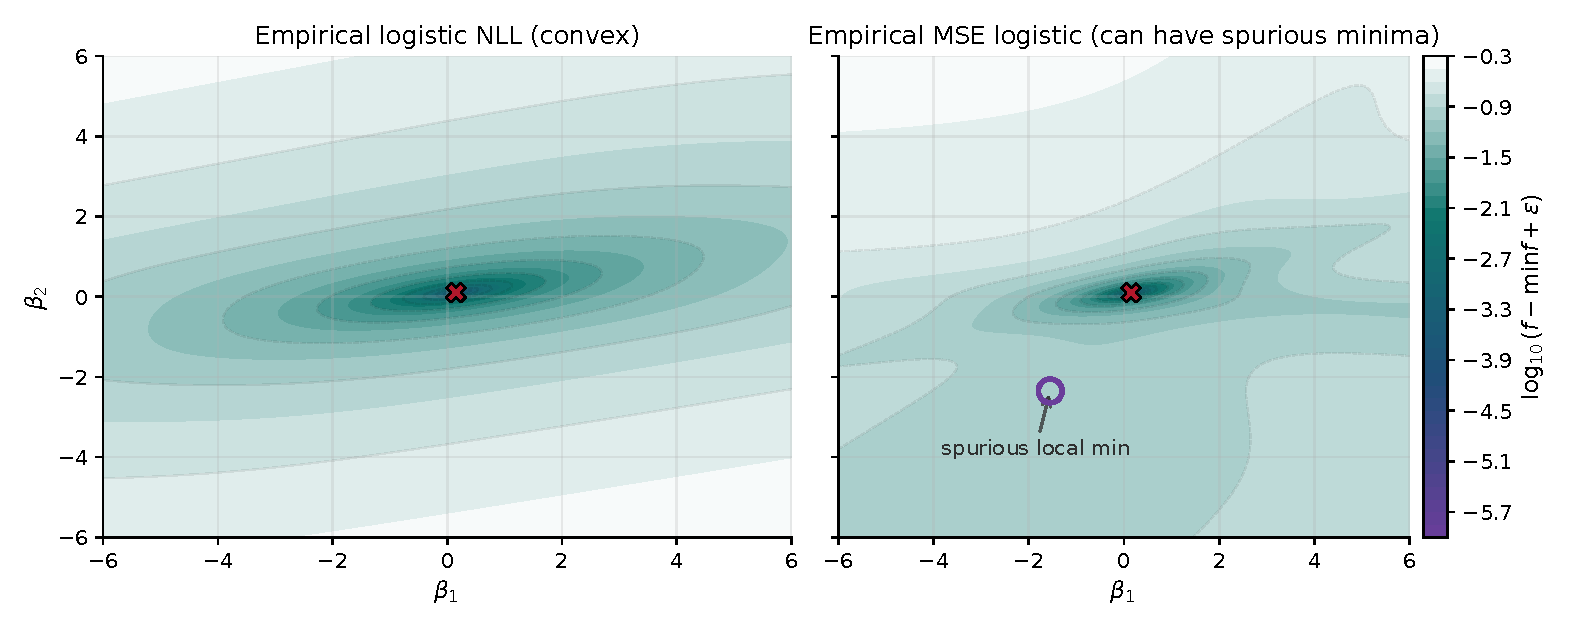
\includegraphics[width=\textwidth]{figures/handouts/convexity_optimization/fig_logistic_empirical_spurious}
  \caption{Empirical logistic landscapes on the dataset in \Cref{ex:logistic-empirical-spurious}.
  The plots show $\log_{10}(f-\min f+\varepsilon)$ for each objective.
  The red X marks the global minimizer in each panel.
  Left: the NLL is convex (one basin).
  Right: the squared-loss objective can have a spurious local minimum (circled), so a local method can get stuck.}
  \label{fig:logistic-empirical-spurious}
\end{figure}

\begin{figure}[t]
  \centering
  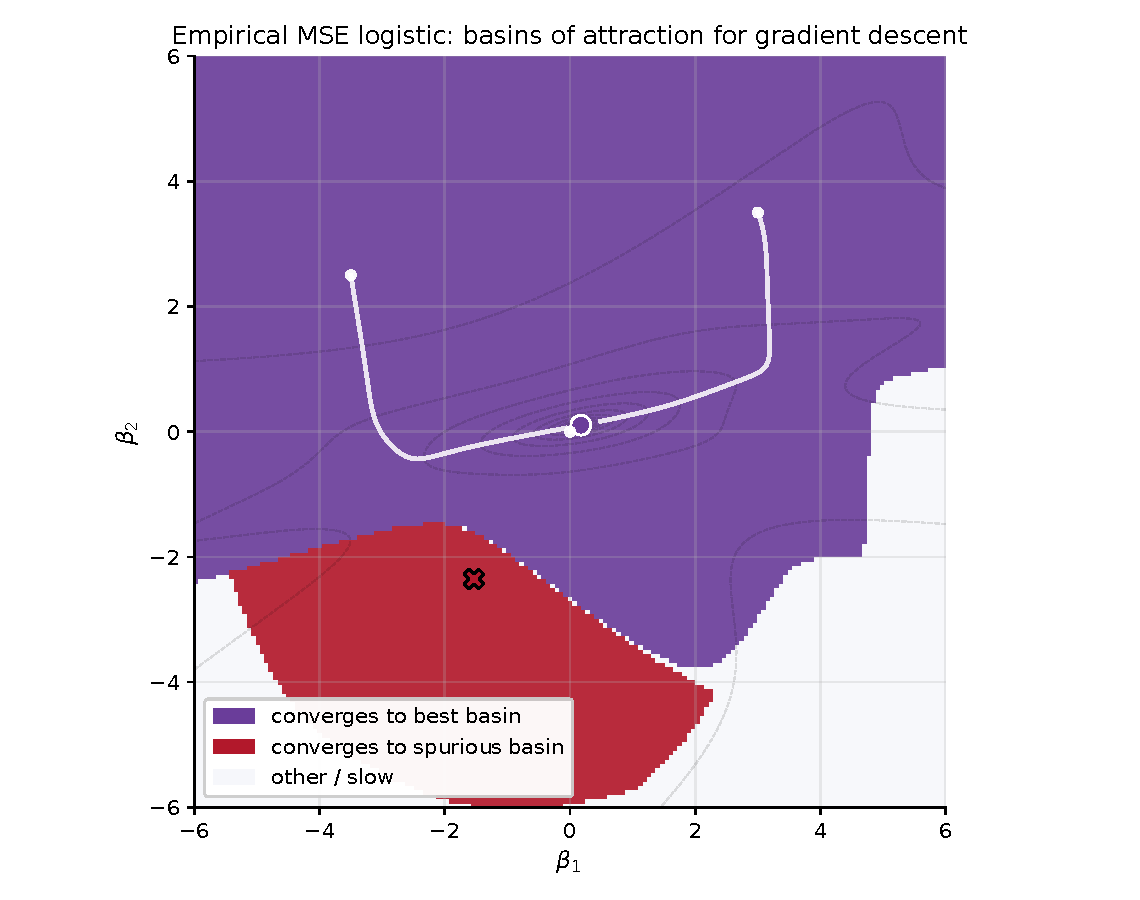
\includegraphics[width=0.92\textwidth]{figures/handouts/convexity_optimization/fig_logistic_empirical_basins}
  \caption{Basins of attraction for gradient descent on the empirical MSE-logistic objective in \Cref{ex:logistic-empirical-spurious}.
  The purple dot and red X mark the two local minimizers.
  Each initialization is colored by which local minimizer fixed-step GD (with $\eta=0.6$) converges to, and the overlaid paths show a few representative trajectories.}
  \label{fig:logistic-empirical-basins}
\end{figure}

Now assume a realizable population model:
\[
Y\mid X=x \sim \mathrm{Bernoulli}(p^\star(x)),
\qquad
p^\star(x) = \sigma(x^\top\beta^\star).
\]
Then the expected squared loss decomposes as
\[
\E\big[(Y-\sigma(X^\top\beta))^2\mid X\big]
= p^\star(X)(1-p^\star(X)) + \big(p^\star(X)-\sigma(X^\top\beta)\big)^2,
\]
so (up to an additive constant) the population objective becomes
\begin{equation}
R(\beta) = \E\big[(\sigma(X^\top\beta)-\sigma(X^\top\beta^\star))^2\big].
\label{eq:logistic-pop-risk}
\end{equation}

\begin{proposition}[One-point monotonicity in the realizable population squared-loss risk]
\label{prop:logistic-pop-one-point}
Assume $\E[\norm{X}_2]<\infty$, and let $R$ be as in \eqref{eq:logistic-pop-risk}. Then for all $\beta$,
\begin{equation}
\ip{\nabla R(\beta)}{\beta-\beta^\star} \ge 0.
\label{eq:one-point}
\end{equation}
In particular, along any ray $\beta(t)=\beta^\star+t(\beta-\beta^\star)$, the function $t\mapsto R(\beta(t))$ is nondecreasing for $t\ge 0$.
\end{proposition}

The next exercise isolates the population monotonicity calculation; structurally it plays the same role as the first-order convexity arguments in the Optimization unit.
\begin{exercise}[One-point monotonicity for realizable MSE-logistic]
\label{ex:logistic-one-point}
Prove \Cref{prop:logistic-pop-one-point}.
Let $\eta=X^\top\beta$ and $\eta^\star=X^\top\beta^\star$.
\begin{enumerate}[leftmargin=*]
  \item Differentiate under the expectation in \eqref{eq:logistic-pop-risk} to show that
  \[
  \nabla R(\beta)
  =2\,\E\Big[(\sigma(\eta)-\sigma(\eta^\star))\,\sigma'(\eta)\,X\Big].
  \]
  \item Show that
  \[
  \ip{\nabla R(\beta)}{\beta-\beta^\star}
  =2\,\E\Big[\sigma'(\eta)\,(\sigma(\eta)-\sigma(\eta^\star))(\eta-\eta^\star)\Big],
  \]
  and conclude it is nonnegative using only that $\sigma$ is increasing and $\sigma'\ge 0$.
  \item Deduce the ray-monotonicity statement by differentiating $g(t)=R(\beta^\star+t(\beta-\beta^\star))$.
\end{enumerate}
\end{exercise}

\SolutionBox[14]{%
\emph{Part (1).}
Differentiate \eqref{eq:logistic-pop-risk} under the expectation:
\[
R(\beta)=\E\big[(\sigma(X^\top\beta)-\sigma(X^\top\beta^\star))^2\big].
\]
Using the chain rule, $\nabla_\beta\sigma(X^\top\beta)=\sigma'(X^\top\beta)\,X$, hence
\[
\nabla R(\beta)
=2\,\E\Big[(\sigma(\eta)-\sigma(\eta^\star))\,\sigma'(\eta)\,X\Big],
\qquad
\eta=X^\top\beta,\ \eta^\star=X^\top\beta^\star.
\]

\emph{Part (2).}
Take the inner product with $(\beta-\beta^\star)$ and use $\ip{X}{\beta-\beta^\star}=\eta-\eta^\star$:
\[
\ip{\nabla R(\beta)}{\beta-\beta^\star}
=2\,\E\Big[\sigma'(\eta)\,(\sigma(\eta)-\sigma(\eta^\star))(\eta-\eta^\star)\Big].
\]
Since $\sigma'(\eta)\ge 0$ and $\sigma$ is increasing, we have
$(\sigma(\eta)-\sigma(\eta^\star))(\eta-\eta^\star)\ge 0$ pointwise.
Therefore the integrand is pointwise nonnegative, and the expectation is nonnegative as claimed.

\emph{Part (3) (ray monotonicity).}
For the ray $\beta(t)=\beta^\star+t(\beta-\beta^\star)$, define $g(t)=R(\beta(t))$.
By the chain rule,
\[
g'(t)=\ip{\nabla R(\beta(t))}{\beta-\beta^\star}\ge 0,
\]
so $t\mapsto R(\beta(t))$ is nondecreasing for $t\ge 0$.
(The argument uses only that the link is increasing with nonnegative derivative, so it holds for any such link function.)%
}

\begin{corollary}[Realizable population MSE-logistic has no spurious local minima]
\label{cor:logistic-pop-no-spurious}
Under the assumptions of \Cref{prop:logistic-pop-one-point}, every local minimizer of the realizable population risk $R$ in \eqref{eq:logistic-pop-risk} is global.
If in addition $\E[XX^\top]\succ 0$, then the unique global minimizer is $\beta^\star$.
\end{corollary}

\begin{exercise}[Stationarity + one-point monotonicity $\Rightarrow$ no spurious local minima]
\label{ex:logistic-one-point-no-spurious}
Prove \Cref{cor:logistic-pop-no-spurious} from \Cref{prop:logistic-pop-one-point}.
\begin{enumerate}[leftmargin=*]
  \item Let $\bar\beta$ be a local minimizer. Since $R$ is differentiable, $\nabla R(\bar\beta)=0$.
  Combine this with \Cref{eq:one-point} to show that
  \[
    0
    = \ip{\nabla R(\bar\beta)}{\bar\beta-\beta^\star}
    = 2\,\E\Big[\sigma'(\bar\eta)\,(\sigma(\bar\eta)-\sigma(\eta^\star))(\bar\eta-\eta^\star)\Big],
  \]
  where $\bar\eta=X^\top\bar\beta$ and $\eta^\star=X^\top\beta^\star$.
  Conclude that $\sigma(X^\top\bar\beta)=\sigma(X^\top\beta^\star)$ almost surely.
  \item Deduce that $R(\bar\beta)=0$, so $\bar\beta$ is a global minimizer.
  \item For uniqueness: show that if $R(\beta)=0$, then $X^\top(\beta-\beta^\star)=0$ almost surely, and deduce $\beta=\beta^\star$ under $\E[XX^\top]\succ 0$.
\end{enumerate}
\end{exercise}

\SolutionBox[14]{%
\emph{Part (1).}
Let $\bar\beta$ be a local minimizer of the differentiable function $R$.
Then $\nabla R(\bar\beta)=0$.
Applying \Cref{prop:logistic-pop-one-point} at $\beta=\bar\beta$ gives
\[
0
= \ip{\nabla R(\bar\beta)}{\bar\beta-\beta^\star}
= 2\,\E\Big[\sigma'(\bar\eta)\,(\sigma(\bar\eta)-\sigma(\eta^\star))(\bar\eta-\eta^\star)\Big],
\qquad \bar\eta=X^\top\bar\beta,\ \eta^\star=X^\top\beta^\star.
\]
The integrand is pointwise nonnegative because $\sigma'(\bar\eta)\ge 0$ and $\sigma$ is increasing, so the expectation can vanish only if the integrand is zero almost surely.
Since $\sigma'(z)>0$ for every finite $z$, this implies
\[
(\sigma(\bar\eta)-\sigma(\eta^\star))(\bar\eta-\eta^\star)=0
\qquad\text{almost surely.}
\]
Because $\sigma$ is strictly increasing, the product above is zero if and only if $\bar\eta=\eta^\star$, equivalently $\sigma(X^\top\bar\beta)=\sigma(X^\top\beta^\star)$ almost surely.

\emph{Part (2).}
If $\sigma(X^\top\bar\beta)=\sigma(X^\top\beta^\star)$ almost surely, then the integrand in \eqref{eq:logistic-pop-risk} vanishes almost surely, so
\[
R(\bar\beta)=\E\big[(\sigma(X^\top\bar\beta)-\sigma(X^\top\beta^\star))^2\big]=0.
\]
Since $R(\beta^\star)=0$ as well, $\bar\beta$ is a global minimizer.

\emph{Part (3) (uniqueness).}
If $R(\beta)=0$, then
\[
\E\big[(\sigma(X^\top\beta)-\sigma(X^\top\beta^\star))^2\big]=0,
\]
so $\sigma(X^\top\beta)=\sigma(X^\top\beta^\star)$ almost surely.
Since $\sigma$ is strictly increasing, this implies $X^\top(\beta-\beta^\star)=0$ almost surely.
Taking expectations yields
$(\beta-\beta^\star)^\top\E[XX^\top](\beta-\beta^\star)=0$.
If $\E[XX^\top]\succ 0$, then the quadratic form is strictly positive unless $\beta=\beta^\star$, so $\beta^\star$ is the unique global minimizer.%
}

The population MSE-logistic risk is nonconvex, but it still has the simple geometry that moving away from $\beta^\star$ does not help along any ray from $\beta^\star$.
This is qualitatively different from objectives like ecological logistic regression (\Cref{sec:ecological-logistic}), where aggregation introduces intrinsic nonconvexity and the landscape can have many distinct basins even under a clean population model.

Even with this benign global geometry, gradient descent can be slow because of saturation and flat plateaus.
The one-point monotonicity in \Cref{prop:logistic-pop-one-point} is a global geometry guarantee, but it is not a rate guarantee.
Far from $\beta^\star$, the squared-loss logistic objective can become very flat because the logistic link saturates:
$\sigma(z)\to 0$ or $1$ and $\sigma'(z)\to 0$ as $|z|\to\infty$.
The squared-loss gradient carries a factor of $\sigma'(X^\top\beta)$, so when the model is very confident (large $|X^\top\beta|$), the gradient can be tiny even if the objective value is not close to its minimum.
This mirrors the ``confidence weights'' story for convex NLL objectives:
in logistic NLL, curvature is largest near the decision boundary, while very confident points contribute little.
For squared loss, that same saturation suppresses the \emph{descent signal} itself, producing plateaus where $\norm{\nabla R(\beta)}_2$ is small even though $R(\beta)-R(\beta^\star)$ is not.

\begin{proposition}[Realizable squared-loss logistic: arbitrarily flat far from $\beta^\star$]
\label{prop:logistic-pop-flat}
Assume $\E[\norm{X}_2]<\infty$ and let $R$ be the realizable population risk \eqref{eq:logistic-pop-risk}.
Define $g(t)=R(t\beta^\star)$ for $t\ge 1$.
Then:
\begin{enumerate}[leftmargin=*]
  \item $g$ is nondecreasing on $[1,\infty)$ and converges to a finite limit $g(\infty)$.
  \item $\lim_{t\to\infty} g'(t)=0$ and $\lim_{t\to\infty}\norm{\nabla R(t\beta^\star)}_2=0$.
  \item If $\Pr(X^\top\beta^\star\neq 0)>0$, then $g(\infty)>0$.
\end{enumerate}
In particular, there are directions along which the landscape becomes arbitrarily flat even though the excess risk stays bounded away from $0$.
\end{proposition}

\emph{Proof idea.} See Exercise~\ref{ex:logistic-plateau}.

\begin{exercise}[Prove the plateau]
\label{ex:logistic-plateau}
In the realizable population model, let $g(t)=R(t\beta^\star)$ for $t\ge 1$.
\begin{enumerate}[leftmargin=*]
  \item Show that
  \[
    g'(t)=2\,\E\big[(\sigma(t\eta^\star)-\sigma(\eta^\star))\,\sigma'(t\eta^\star)\,\eta^\star\big],
    \qquad \eta^\star=X^\top\beta^\star,
  \]
  and conclude that $g$ is nondecreasing (hence $g(t)\to g(\infty)$ since $0\le g(t)\le 1$).
  \item Show that $g'(t)\to 0$ and $\nabla R(t\beta^\star)\to 0$ as $t\to\infty$.
  Interpret this as: \emph{without} a PL/strong-convexity-type condition, small gradient does not imply near-optimality.
  \item Assume $\Pr(\eta^\star\neq 0)>0$.
  Show that $g(\infty)>0$.
\end{enumerate}
\end{exercise}

\SolutionBox[12]{%
Write $\eta^\star=X^\top\beta^\star$ so that $g(t)=\E[(\sigma(t\eta^\star)-\sigma(\eta^\star))^2]$.

\emph{Part (1).}
Differentiate under the expectation:
by the chain rule,
\[
\frac{d}{dt}\sigma(t\eta^\star)=\sigma'(t\eta^\star)\,\eta^\star,
\]
so
\[
g'(t)
=\E\Big[2(\sigma(t\eta^\star)-\sigma(\eta^\star))\cdot \sigma'(t\eta^\star)\,\eta^\star\Big]
=2\,\E\big[(\sigma(t\eta^\star)-\sigma(\eta^\star))\,\sigma'(t\eta^\star)\,\eta^\star\big].
\]
For $t\ge 1$, $\sigma(t\eta^\star)-\sigma(\eta^\star)$ has the same sign as $(t-1)\eta^\star$ since $\sigma$ is increasing.
Because $\sigma'\ge 0$, the integrand is pointwise nonnegative, hence $g'(t)\ge 0$ and $g$ is nondecreasing.
Since $g(t)\in[0,1]$, it follows that $g(t)\to g(\infty)$ for some finite limit $g(\infty)$.

\emph{Part (2).}
For each fixed $\eta^\star\neq 0$, we have $t\eta^\star\to \pm\infty$ and therefore $\sigma'(t\eta^\star)\to 0$ as $t\to\infty$.
Also,
\[
\big|(\sigma(t\eta^\star)-\sigma(\eta^\star))\,\sigma'(t\eta^\star)\,\eta^\star\big|
\le \sigma'(0)\,|\eta^\star|
\le \sigma'(0)\,\norm{\beta^\star}_2\,\norm{X}_2,
\]
which is integrable since $\E[\norm{X}_2]<\infty$.
We will use the following standard fact: if random variables $Z_t$ satisfy $|Z_t|\le W$ with $\E[W]<\infty$ and $Z_t\to 0$ almost surely, then $\E[Z_t]\to 0$.
Applying this fact here gives $g'(t)\to 0$ as $t\to\infty$.

\smallskip
Similarly, differentiating \eqref{eq:logistic-pop-risk} gives
\[
\nabla R(t\beta^\star)
=2\,\E\big[(\sigma(t\eta^\star)-\sigma(\eta^\star))\,\sigma'(t\eta^\star)\,X\big].
\]
The integrand norm is bounded by $2\sigma'(0)\norm{X}_2$, and for each fixed $X$ the factor $\sigma'(t\eta^\star)$ tends to $0$ (or the bracketed term vanishes when $\eta^\star=0$), so the same reasoning lets us pass the limit through the expectation and conclude $\nabla R(t\beta^\star)\to 0$.

\emph{Part (3).}
As $t\to\infty$ we have $\sigma(t\eta^\star)\to 1$ when $\eta^\star>0$, $\sigma(t\eta^\star)\to 0$ when $\eta^\star<0$, and $\sigma(t\eta^\star)=\sigma(\eta^\star)=1/2$ when $\eta^\star=0$.
Since $0\le (\sigma(t\eta^\star)-\sigma(\eta^\star))^2\le 1$, we can apply the same fact (with $W=1$) to pass the limit through the expectation and obtain
\[
g(\infty)=\E\Big[(1-\sigma(\eta^\star))^2\mathbf{1}\{\eta^\star>0\} + \sigma(\eta^\star)^2\mathbf{1}\{\eta^\star<0\}\Big].
\]
If $\Pr(\eta^\star\neq 0)>0$, then the integrand is strictly positive on $\{\eta^\star\neq 0\}$, so $g(\infty)>0$.

Along this ray, the risk can remain bounded away from $0$ while the gradient (and directional derivative) goes to $0$.
Without a condition like PL/strong convexity, a small gradient does not by itself certify near-optimality.
}

Conditions like strong convexity or the PL inequality (\Cref{def:pl-inequality}) prevent this phenomenon: they rule out large flat regions away from the optimum by relating gradient size to suboptimality.
\Cref{prop:logistic-pop-flat} shows the realizable squared-loss logistic risk does not have such a global guarantee in general.

In the realizable population model, the one-point monotonicity in \Cref{prop:logistic-pop-one-point} is a \emph{global} geometric statement.
To get an actual rate for gradient descent, we also need a \emph{local curvature} condition near $\beta^\star$.
One simple sufficient condition is bounded features, which implies local strong convexity (hence a linear rate) around the optimum.

\begin{proposition}[Local linear convergence of gradient descent near $\beta^\star$]
\label{prop:logistic-pop-local-rate}
Assume $\E[XX^\top]\succeq \lambda I_d$ and $\norm{X}_2\le R$ almost surely for some $\lambda,R>0$.
Then at $\beta^\star$,
\[
\Hess R(\beta^\star)\succeq m_0 I_d,
\qquad
m_0 = 2\,\sigma'(R\norm{\beta^\star}_2)^2\,\lambda,
\]
and there exist $r>0$ and constants $0<m\le L<\infty$ such that the population risk $R$ in \eqref{eq:logistic-pop-risk} is $m$-strongly convex and $L$-smooth on the ball $\{\beta:\ \norm{\beta-\beta^\star}_2\le r\}$.
Consequently, gradient descent with step size $1/L$ initialized in this ball satisfies
\[
R(\beta^{(k)})-R(\beta^\star)
\le \left(1-\frac{m}{L}\right)^k\bigl(R(\beta^{(0)})-R(\beta^\star)\bigr)
\qquad\text{(see \citealp[\S9.3]{boyd_vandenberghe_2004_convex}).}
\]
\end{proposition}

\begin{proof}
Differentiate \eqref{eq:logistic-pop-risk} twice.
At $\beta=\beta^\star$, the cross term vanishes and the Hessian simplifies to
\[
\Hess R(\beta^\star)=2\,\E\big[\sigma'(X^\top\beta^\star)^2\,XX^\top\big].
\]
Since $\norm{X^\top\beta^\star}\le \norm{X}_2\norm{\beta^\star}_2\le R\norm{\beta^\star}_2$ almost surely, we have
$\sigma'(X^\top\beta^\star)\ge \sigma'(R\norm{\beta^\star}_2)>0$ almost surely (since $\sigma'$ is even and decreases with $|z|$), hence
\[
\Hess R(\beta^\star)\succeq 2\,\sigma'(R\norm{\beta^\star}_2)^2\,\E[XX^\top]\succeq 2\,\sigma'(R\norm{\beta^\star}_2)^2\,\lambda I_d.
\]
This is the claimed bound with $m_0=2\,\sigma'(R\norm{\beta^\star}_2)^2\,\lambda$.
Because $R$ is twice continuously differentiable and $\norm{X}_2\le R$ almost surely, $\Hess R(\beta)$ varies continuously in $\beta$ and is bounded on compact sets.
Therefore, on a sufficiently small ball around $\beta^\star$, the Hessian is bounded below by (say) $\tfrac12 m_0 I_d$ and above by $L I_d$ for some finite $L$, which gives local strong convexity and smoothness.
The linear convergence rate for gradient descent on an $m$-strongly convex and $L$-smooth function is standard (cited above).
\end{proof}

Under misspecification, hard multimodality can return.
If $p^\star(x)$ is not representable as $\sigma(x^\top\beta)$ (e.g.\ marginalizing over latent classes can yield mixtures of logits), then \eqref{eq:one-point} need not hold, and the population squared-loss risk can become bimodal with spurious local minima.
Benign global geometry often hinges on model and data assumptions.
This is one reason MLE (convex NLL) is often more stable than squared-loss fitting in logistic-type binary regression models.

\begin{example}[Misspecification can create a spurious local minimum for squared-loss logistic regression]
\label{ex:logistic-misspecified-spurious}
Consider a 1D feature $X$ that takes values $\{-2,-1,1,2\}$ with equal probability, and parameterize $\beta=(\beta_0,\beta_1)$ so that $q_\beta(x)=\sigma(\beta_0+\beta_1 x)$.
Let the true conditional probabilities be
\[
p^\star(-2)=0.49,\quad p^\star(-1)=0.87,\quad p^\star(1)=0.92,\quad p^\star(2)=0.36.
\]
This $p^\star$ is not representable as $q_\beta$, since it is not monotone in $x$.

For the population squared-loss risk $R_{\mathrm{MSE}}(\beta)=\E[(q_\beta(X)-p^\star(X))^2]$, a direct evaluation shows two distinct basins:
numerically, evaluating $R_{\mathrm{MSE}}$ on a grid reveals a global minimizer and a spurious local minimizer.
See \Cref{fig:logistic-landscape-2d}.
\end{example}

\begin{figure}[t]
  \centering
  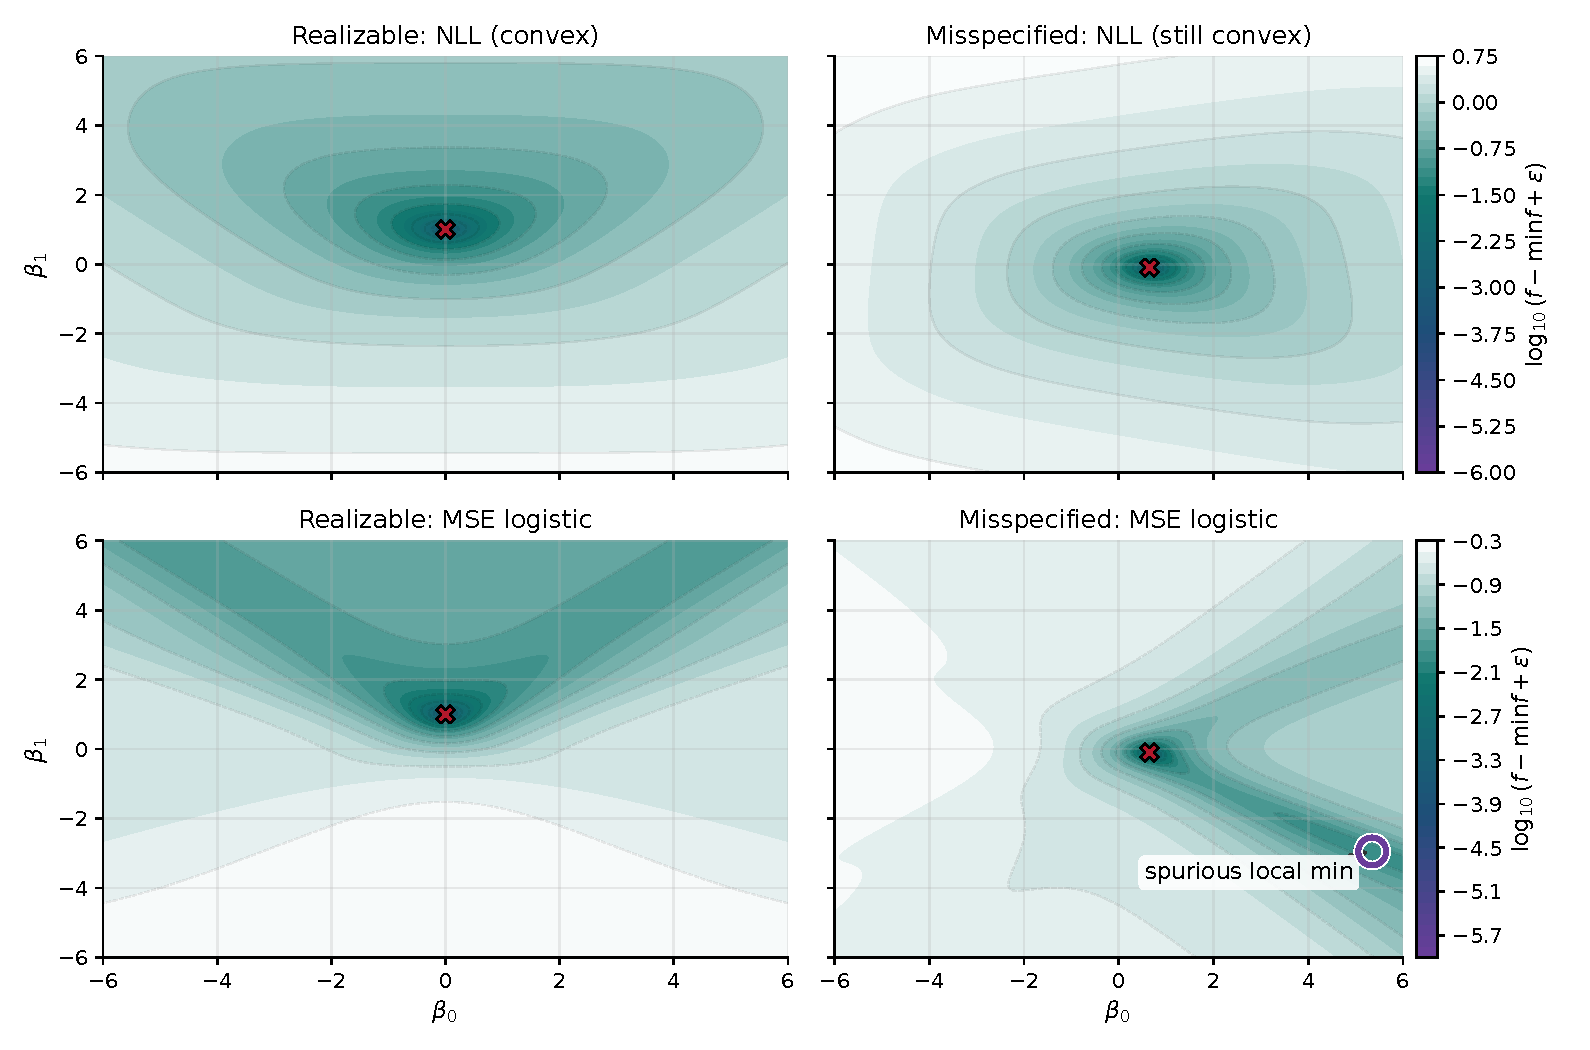
\includegraphics[width=\textwidth]{figures/handouts/convexity_optimization/fig_logistic_landscape_2d}
  \caption{A consistent contourf view of logistic landscapes in a 2D parameterization $\beta=(\beta_0,\beta_1)$.
  The plots show $\log_{10}(f-\min f+\varepsilon)$ for each objective, which makes basins comparable across panels.
  The red X marker indicates the global minimizer in each panel; in the bottom-right plot, the circled point is a spurious local minimum.
  In this example, the NLL landscape is unimodal in both realizable and misspecified settings, while the squared-loss landscape can develop extra basins under misspecification.}
  \label{fig:logistic-landscape-2d}
\end{figure}

% ------------------------------------------------------------
Example~I separates three distinct regimes.
Empirical MSE-logistic can create spurious basins; the realizable population risk has no spurious local minima but can still be slow because of broad plateaus; and misspecification can bring back genuinely wrong stable basins.
The response depends on the regime: use a stable objective when possible, use damping or line search when curvature is unreliable, and use restarts or stronger initializations when multiple basins are present.

% ------------------------------------------------------------
\section[Example II (phase retrieval)]{Example II: multimodality from symmetry, but only global optima in phase retrieval}
\label{sec:phase-retrieval}

In coherent diffraction imaging, optics, and astronomy, sensors measure intensities and lose phase.
A canonical real model is \emph{phase retrieval}:
\[
y_i = (a_i^\top x^\star)^2,\qquad i=1,\dots,m,
\]
where $x^\star\in\R^d$ is the unknown signal and $a_i$ are known sensing vectors.
A standard nonconvex least-squares objective is
\begin{equation}
F(x)=\frac{1}{4m}\sum_{i=1}^m\big((a_i^\top x)^2 - y_i\big)^2.
\label{eq:phase-empirical}
\end{equation}
This objective is nonconvex for structural reasons (it involves squares of linear forms),
and it is \emph{inherently} multimodal because $x^\star$ and $-x^\star$ generate the same data.

Like squared-loss logistic regression, phase retrieval is a smooth, nonconvex least-squares objective.
But here the nonconvexity is driven primarily by a \emph{symmetry}: $x^\star$ and $-x^\star$ generate the same data.
In population (for Gaussian designs), this symmetry produces multiple global optima but \emph{no} suboptimal local minima; the remaining stationary points are saddles.
This is ``benign'' nonconvexity (a strict-saddle picture), and it contrasts with ecological logistic regression (\Cref{sec:ecological-logistic}), where aggregation creates intrinsic nonconvexity and can lead to many distinct basins.
This ``benign geometry'' picture (multiple equivalent global minimizers; strict saddles elsewhere) appears broadly in modern tractable nonconvex problems; see \citet[\S2]{sun_qu_wright_2015_nonconvex_not_scary} and \citet[\S1]{zhang_qu_wright_2020_symmetry_geometry}.

\begin{figure}[t]
  \centering
  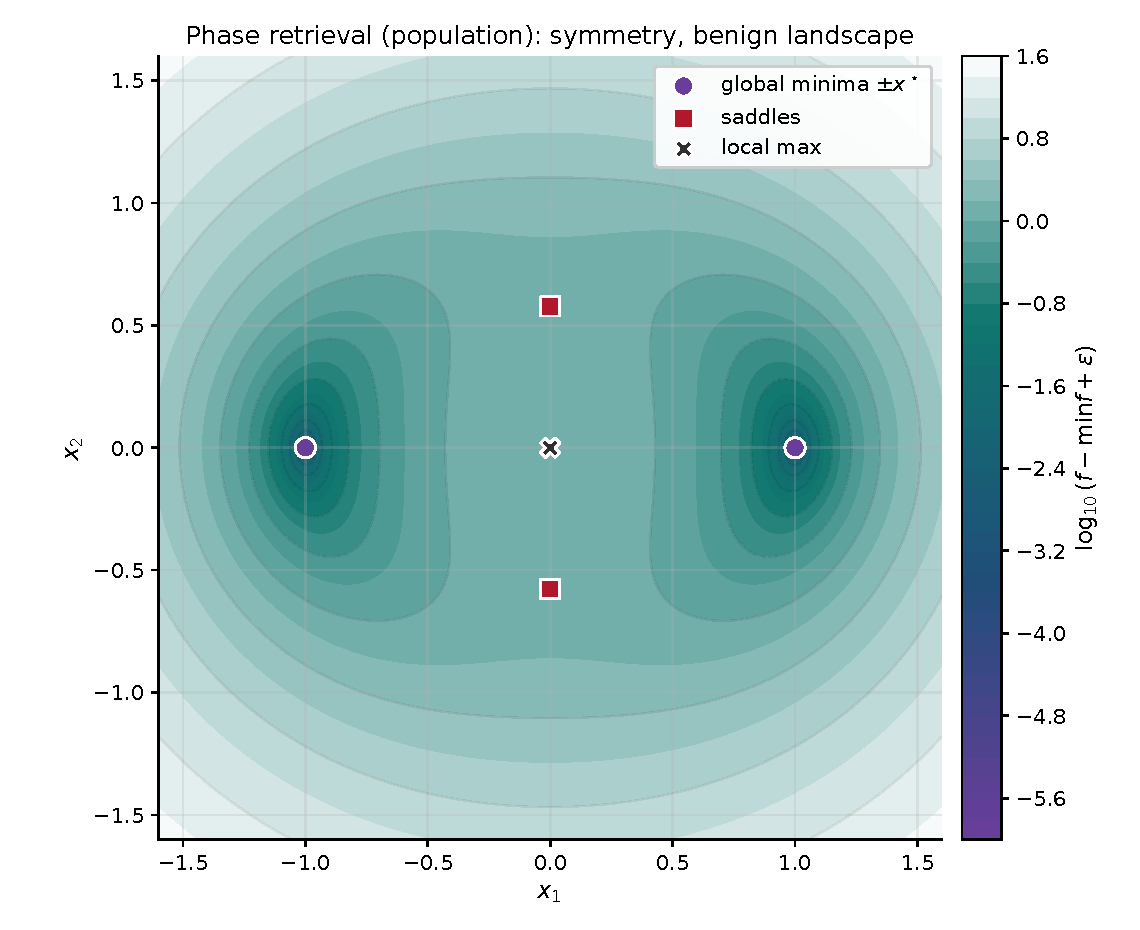
\includegraphics[width=0.86\textwidth]{figures/handouts/convexity_optimization/fig_phase_retrieval_landscape}
  \caption{Population phase retrieval in $d=2$: the landscape is nonconvex and symmetric ($x\sim -x$), but the only local minima are the two global minima $\pm x^\star$; other critical points are saddles or a local maximum at the origin.}
  \label{fig:phase-retrieval-landscape}
\end{figure}

For a clean population model, assume $a\sim N(0,I_d)$ and consider the \emph{population} objective
\begin{equation}
  f(x)=\frac12\,\E\Big[\big((a^\top x)^2 - (a^\top x^\star)^2\big)^2\Big].
  \label{eq:phase-pop}
\end{equation}

\begin{proposition}[Population phase retrieval: nonconvex but no spurious local minima]
\label{prop:phase-retrieval-benign}
For $f$ in \eqref{eq:phase-pop},
\begin{equation}
  f(x)
  =\frac{3}{2}\norm{x}^4 - \norm{x}^2\norm{x^\star}^2 - 2\ip{x}{x^\star}^2 + \frac{3}{2}\norm{x^\star}^4,
  \label{eq:phase-pop-closed-form}
\end{equation}
and the stationary points are:
\begin{enumerate}[leftmargin=*]
  \item global minima $x=\pm x^\star$ (value $0$),
  \item a local maximum at $x=0$,
  \item a saddle set $\{x:\ x\perp x^\star,\ \norm{x}=\norm{x^\star}/\sqrt{3}\}$.
\end{enumerate}
In particular, every local minimum is global.
\end{proposition}

\begin{exercise}[Phase retrieval: derive and classify the population stationary points]
\label{ex:phase-pop-derivation}
Prove \Cref{prop:phase-retrieval-benign}.
\begin{enumerate}[leftmargin=*]
  \item Expand \eqref{eq:phase-pop} and use the Gaussian fourth-moment identities
  \[
  \E[(a^\top u)^4]=3\norm{u}^4,
  \qquad
  \E[(a^\top u)^2(a^\top v)^2]=\norm{u}^2\norm{v}^2 + 2\ip{u}{v}^2,
  \]
  to obtain \eqref{eq:phase-pop-closed-form}.
  \item Differentiate \eqref{eq:phase-pop-closed-form} to get an explicit formula for $\nabla f(x)$.
  \item Solve $\nabla f(x)=0$ by decomposing $x=\alpha x^\star + u$ with $u\perp x^\star$.
  \item Classify the stationary points as global minima, a local maximum, and a saddle set.
\end{enumerate}
\end{exercise}

\SolutionBox[22]{%
\emph{Part (1) (closed form).}
Expanding the square in \eqref{eq:phase-pop} gives
\[
f(x)
=\frac12\,\E\big[(a^\top x)^4\big]
\;-\;\E\big[(a^\top x)^2(a^\top x^\star)^2\big]
\;+\;\frac12\,\E\big[(a^\top x^\star)^4\big].
\]
Apply the stated Gaussian fourth-moment identities with $u=x$ and $v=x^\star$ to get
\[
\E[(a^\top x)^4]=3\norm{x}^4,\qquad
\E[(a^\top x^\star)^4]=3\norm{x^\star}^4,
\]
and
\[
\E[(a^\top x)^2(a^\top x^\star)^2]=\norm{x}^2\norm{x^\star}^2 + 2\ip{x}{x^\star}^2.
\]
Substituting yields \eqref{eq:phase-pop-closed-form}.

\emph{Part (2) (gradient).}
Differentiate \eqref{eq:phase-pop-closed-form}:
\[
\nabla f(x)
= 6\norm{x}^2 x - 2\norm{x^\star}^2 x - 4\ip{x}{x^\star}x^\star
= (6\norm{x}^2-2\norm{x^\star}^2)x - 4\ip{x}{x^\star}x^\star.
\]

\emph{Part (3) (stationary points).}
Let $r=\norm{x^\star}_2$ and decompose $x=\alpha x^\star + u$ with $u\perp x^\star$.
Then $\ip{x}{x^\star}=\alpha r^2$ and $\norm{x}^2=\alpha^2r^2+\norm{u}^2$.
Setting $\nabla f(x)=0$ and matching the $u$ and $x^\star$ components gives
\[
(6\norm{x}^2-2r^2)\,u=0,
\qquad
\alpha\,(6\norm{x}^2-6r^2)=0.
\]
If $u=0$, then either $\alpha=0$ (so $x=0$) or $\norm{x}^2=r^2$ (so $\alpha=\pm 1$ and $x=\pm x^\star$).
If $u\neq 0$, then the first equation forces $\norm{x}^2=r^2/3$, and the second forces $\alpha=0$, hence
$x\perp x^\star$ and $\norm{x}=r/\sqrt{3}$.
This gives exactly the stationary-point list in \Cref{prop:phase-retrieval-benign}.

\emph{Part (4) (classification).}
Since $f$ in \eqref{eq:phase-pop} is an expectation of a square, $f(x)\ge 0$ for all $x$.
Also $f(\pm x^\star)=0$, so $\pm x^\star$ are global minima.

For $x=0$, the expansion \eqref{eq:phase-pop-closed-form} shows
\[
f(0)-f(x)= r^2\norm{x}^2 + 2\ip{x}{x^\star}^2 - \frac{3}{2}\norm{x}^4,
\]
which is strictly positive for all sufficiently small $x\neq 0$ (the quadratic term dominates), so $x=0$ is a local maximum.

Finally, if $x\perp x^\star$ and $\norm{x}=r/\sqrt{3}$, then the univariate restriction $t\mapsto f(x+t x^\star)$ has negative second derivative at $t=0$, so there is a direction of negative curvature.
Hence these points are saddles, and every local minimum is global.%
}

This is symmetry-driven nonconvexity with a strict-saddle geometry:
every non-optimal stationary point has a direction of negative curvature.

Phase retrieval is typically approached via the two-stage template in \Cref{alg:two-stage-template}:
use a cheap global initializer, then run a local method.
In the Gaussian model, there is a clean way to build a provably good direction estimate from a simple moment identity.
Assume the noiseless Gaussian design model $a_i \stackrel{\mathrm{iid}}{\sim} N(0,I_d)$ with measurements $y_i=(a_i^\top x^\star)^2$.
Define the \emph{spectral matrix}
\[
  Y = \frac{1}{m}\sum_{i=1}^m y_i a_i a_i^\top.
\]
Also define the radius estimate
\[
  \hat r^2 = \frac{1}{m}\sum_{i=1}^m y_i,
\]
which satisfies $\E[\hat r^2]=\norm{x^\star}_2^2$.
If $\hat u$ is a unit-norm top eigenvector of $Y$, then the standard spectral initializer is $x^{(0)}=\hat r\,\hat u$.

The next proposition explains why this initialization is reasonable.
It shows that (i) the population matrix $\E[Y]$ has a unique leading eigenvector in the $x^\star$ direction, and (ii) if the empirical $Y$ is close to $\E[Y]$ in operator norm then its leading eigenvector must be close to $\pm x^\star/\norm{x^\star}_2$.
(Here $\norm{M}_{\mathrm{op}}$ denotes the operator norm, i.e.\ the largest absolute eigenvalue for a symmetric matrix $M$.)

\begin{proposition}[Gaussian phase retrieval: why the spectral initializer points at $x^\star$]
\label{prop:phase-spectral-init}
Assume $x^\star\neq 0$, let $a\sim N(0,I_d)$, and set $y=(a^\top x^\star)^2$.
Write $r=\norm{x^\star}_2$ and $u^\star=x^\star/r$.
Define the population matrix
\[
  Y_{\mathrm{pop}} = \E\big[y\,a a^\top\big]
  = \E\big[(a^\top x^\star)^2 a a^\top\big].
\]
Then
\[
  Y_{\mathrm{pop}}=r^2 I_d + 2x^\star(x^\star)^\top,
\]
so the unique leading eigenvector of $Y_{\mathrm{pop}}$ is $u^\star$.
Moreover, if $Y$ is any symmetric matrix satisfying
\[
\norm{Y-Y_{\mathrm{pop}}}_{\mathrm{op}} \le \varepsilon\, r^2
\qquad\text{for some }\varepsilon\in(0,1),
\]
then for every unit-norm leading eigenvector $\hat u$ of $Y$ there exists a sign $s\in\{\pm 1\}$ such that
$\norm{\hat u-su^\star}_2\le \sqrt{2\varepsilon}$.
\end{proposition}

\begin{exercise}[Phase retrieval: why spectral initialization points at $x^\star$]
\label{ex:phase-spectral-spike}
Prove \Cref{prop:phase-spectral-init}.
Conclude that if the empirical matrix $Y$ is close to $Y_{\mathrm{pop}}$ in operator norm, then its top eigenvector is close to $\pm u^\star$ and the spectral initializer $x^{(0)}=\hat r\,\hat u$ is close to $\pm x^\star$.
\emph{Hint:} to compute $Y_{\mathrm{pop}}$, you can either compute entries using the Gaussian fourth-moment identity
$\E[a_i a_j a_k a_\ell]=\delta_{ij}\delta_{k\ell}+\delta_{ik}\delta_{j\ell}+\delta_{i\ell}\delta_{jk}$,
or compute the entries directly by expanding.
For the perturbation bound, compare quadratic forms $v^\top Y v$ and use $|v^\top (Y-Y_{\mathrm{pop}}) v|\le \norm{Y-Y_{\mathrm{pop}}}_{\mathrm{op}}$ for unit $v$.
Finally, explain in a sentence why one expects $\norm{Y-Y_{\mathrm{pop}}}_{\mathrm{op}}$ to be small when $m$ is large in the Gaussian model.
\end{exercise}

\SolutionBox[20]{%
Write $u=x^\star$ and expand $y=(a^\top u)^2=\sum_{k,\ell} u_k u_\ell a_k a_\ell$.
For each entry $(i,j)$,
\[
\E\!\big[y\,a_i a_j\big]
=\sum_{k,\ell} u_k u_\ell\,\E[a_i a_j a_k a_\ell]
=\sum_{k,\ell} u_k u_\ell\bigl(\delta_{ij}\delta_{k\ell}+\delta_{ik}\delta_{j\ell}+\delta_{i\ell}\delta_{jk}\bigr).
\]
The first term gives $\delta_{ij}\sum_k u_k^2=\delta_{ij}\norm{u}_2^2$.
The second and third terms each give $u_i u_j$.
Thus $\E[y\,a_i a_j]=\norm{u}_2^2\,\delta_{ij}+2u_i u_j$, i.e.
$Y_{\mathrm{pop}}=\norm{u}_2^2 I_d + 2uu^\top$.

For eigenvalues, note that $Y_{\mathrm{pop}}u=(\norm{u}_2^2+2\norm{u}_2^2)u=3\norm{u}_2^2 u$.
If $w\perp u$, then $uu^\top w=0$ so $Y_{\mathrm{pop}}w=\norm{u}_2^2 w$.
Hence the unique top eigenspace is $\mathrm{span}\{u\}$.

Let $r=\norm{u}_2$ and $u^\star=u/r$.
Let $\hat u$ be a unit top eigenvector of $Y$.
Write $E=Y-Y_{\mathrm{pop}}$ and assume $\norm{E}_{\mathrm{op}}\le \varepsilon r^2$.
Then
\[
\hat u^\top Y_{\mathrm{pop}} \hat u
= \hat u^\top Y \hat u - \hat u^\top E \hat u
\ge \lambda_{\max}(Y) - \norm{E}_{\mathrm{op}}
\ge (u^\star)^\top Y u^\star - \norm{E}_{\mathrm{op}}
\ge 3r^2 - 2\varepsilon r^2.
\]
On the other hand,
$
\hat u^\top Y_{\mathrm{pop}} \hat u
= r^2 + 2r^2\,|\ip{\hat u}{u^\star}|^2.
$
Combining gives $|\ip{\hat u}{u^\star}|^2\ge 1-\varepsilon$.
Choosing the sign that maximizes the inner product,
\[
\min\{\norm{\hat u-u^\star}_2,\norm{\hat u+u^\star}_2\}^2
=2\bigl(1-|\ip{\hat u}{u^\star}|\bigr)
\le 2\bigl(1-|\ip{\hat u}{u^\star}|^2\bigr)
\le 2\varepsilon.
\]

The matrix $Y$ is an empirical average of i.i.d.\ symmetric matrices with mean $Y_{\mathrm{pop}}$.
To make this quantitative in high dimensions, one uses concentration inequalities for random matrices to bound $\norm{Y-Y_{\mathrm{pop}}}_{\mathrm{op}}$ with high probability; see \citet[\S2.2]{zhang_qu_wright_2020_symmetry_geometry} for discussion and references.
These probability tools are largely orthogonal to our focus here.%
}

Once you have an initialization that is close to $\pm x^\star$, the local stage behaves like the convex story again.
In the Gaussian population objective, $\pm x^\star$ are not only global minima: they are \emph{locally strongly convex} minima, so the standard local strong-convexity analysis from the Optimization unit gives a linear rate while the iterates remain in that neighborhood.

\begin{exercise}[Phase retrieval: local convexity near $\pm x^\star$ in the population objective]
\label{ex:phase-pop-local-strong-convex}
For the population objective $f$ in \eqref{eq:phase-pop-closed-form}, compute the Hessian $\Hess f(x)$ and show that
\[
\Hess f(x^\star)=4\norm{x^\star}_2^2 I_d + 8x^\star(x^\star)^\top.
\]
Deduce the eigenvalues of $\Hess f(x^\star)$ and interpret this as a local condition-number statement near $x^\star$.
\end{exercise}

\SolutionBox[12]{%
Differentiate the gradient formula in the solution to \Cref{ex:phase-pop-derivation}:
for $x\in\R^d$,
\[
\Hess f(x)=12xx^\top + (6\norm{x}_2^2-2\norm{x^\star}_2^2)I_d - 4x^\star(x^\star)^\top.
\]
At $x=x^\star$ this becomes
\[
\Hess f(x^\star)=(12-4)x^\star(x^\star)^\top + 4\norm{x^\star}_2^2 I_d
=8x^\star(x^\star)^\top + 4\norm{x^\star}_2^2 I_d.
\]
Along $u^\star=x^\star/\norm{x^\star}_2$ the eigenvalue is $12\norm{x^\star}_2^2$, and along any direction orthogonal to $x^\star$ the eigenvalue is $4\norm{x^\star}_2^2$.
So near $x^\star$ the population objective is well conditioned (local condition number $3$), which is exactly the regime where local methods behave like in the convex case.%
}

These pieces give the standard Gaussian-model story:
spectral initialization supplies a direction close to $\pm x^\star$, and the local geometry near $\pm x^\star$ is strongly convex, so local methods converge quickly once initialized there.
Rigorous finite-sample analyses follow this template; see \citet[\S2.2]{zhang_qu_wright_2020_symmetry_geometry} and references therein.

Phase retrieval shows a different kind of nonconvexity.
The sign symmetry creates multiple optima, but they are equivalent, and the remaining stationary points are saddles rather than bad local minima.
The right response is therefore not exhaustive global search; it is a coarse initializer, such as a spectral method, followed by local refinement inside the basin of $\pm x^\star$.



% ------------------------------------------------------------
\section[Example III (ecological logistic)]{Example III: hard nonconvexity from aggregation in ecological logistic regression}
\label{sec:ecological-logistic}

In some applications we observe covariates at the unit level but only aggregated outcomes.
For example, we might see covariates $x_{g,1},\dots,x_{g,n_g}$ for individuals in a group (a precinct, a cohort, a batch),
but instead of observing the binary outcomes $Y_{g,i}\in\{0,1\}$ we only observe the group total
\[
Z_g = \sum_{i=1}^{n_g} Y_{g,i}.
\]
Many different binary vectors $(Y_{g,1},\dots,Y_{g,n_g})$ can produce the same total $Z_g$, so the likelihood for $\beta$ must marginalize over a large discrete set of latent ``assignments.''

Assume a logistic model at the unit level:
\[
\Pr(Y_{g,i}=1\mid x_{g,i},\beta)=\sigma(x_{g,i}^\top\beta),
\qquad i=1,\dots,n_g,
\]
with conditional independence across $i$ given the covariates.
Write $p_{g,i}(\beta)=\sigma(x_{g,i}^\top\beta)$.
Then $Z_g$ is a sum of independent but non-identically distributed Bernoulli random variables (a Poisson--binomial model), and the marginal likelihood contains $\binom{n_g}{z_g}$ terms.
The resulting negative log-likelihood is typically nonconvex in $\beta$.
This combinatorial marginalization also creates a separate difficulty that is easy to miss if we focus only on the geometry:
when $n_g$ is large, the likelihood term $\Pr(Z_g=z_g\mid x_{g,1},\dots,x_{g,n_g},\beta)$ can be expensive to evaluate repeatedly inside an optimizer.
The naive computation is literally a sum over $\binom{n_g}{z_g}$ assignments (as in \Cref{ex:eco-logistic-nonconvex}), which is intractable for large groups.
This ``optimization + marginalization'' pattern is common in latent-variable models: hard landscapes and expensive objective evaluations can come together.

An empirical negative log-likelihood objective for $G$ independent groups is
\begin{equation}
  f(\beta)
  =
  -\frac{1}{G}\sum_{g=1}^G \log \Pr(Z_g=z_g \mid x_{g,1},\dots,x_{g,n_g},\beta).
  \label{eq:eco-logistic-obj}
\end{equation}
Two edge cases are instructive.
In the special case where the covariates are constant within each group ($x_{g,i}\equiv x_g$), we have
$Z_g\sim \mathrm{Binomial}(n_g,\sigma(x_g^\top\beta))$, and \eqref{eq:eco-logistic-obj} reduces to the usual convex binomial logistic-regression objective from the Optimization unit.
At the other extreme, if $d=1$ with $\beta=(\beta_0,\beta_1)$ and each group contains covariates in $\pm$ pairs (for every $x$ the value $-x$ appears with the same multiplicity), then the marginal likelihood is symmetric in the slope: it is unchanged under $\beta_1\mapsto -\beta_1$.
This kind of symmetry reflects a genuine non-identifiability from totals alone.

\begin{exercise}[Ecological logistic regression: two easy special cases]
\label{ex:eco-logistic-edge-cases}
\begin{enumerate}[leftmargin=*]
  \item Suppose $x_{g,i}\equiv x_g$ within each group.
  Show that $Z_g\sim \mathrm{Binomial}(n_g,\sigma(x_g^\top\beta))$ and conclude that the corresponding negative log-likelihood is convex in $\beta$.
  \item Assume $d=1$ with $\beta=(\beta_0,\beta_1)$ and suppose the multiset $\{x_1,\dots,x_n\}$ is symmetric: for every $x$ it contains $-x$ with the same multiplicity.
  Show that, for every $z$,
  \[
    \Pr(Z=z\mid x_1,\dots,x_n,(\beta_0,\beta_1))
    =
    \Pr(Z=z\mid x_1,\dots,x_n,(\beta_0,-\beta_1)).
  \]
  Conclude that the likelihood for $\beta_1$ is an even function, so the sign of the slope is not identifiable from $Z$ alone in such a balanced design.
\end{enumerate}
\end{exercise}

\SolutionBox[14]{%
\emph{Part (1).}
If $x_{g,i}\equiv x_g$, then conditional on $x_g$ the unit-level outcomes are i.i.d.\ Bernoulli with success probability $\sigma(x_g^\top\beta)$.
Therefore $Z_g=\sum_{i=1}^{n_g}Y_{g,i}\sim \mathrm{Binomial}(n_g,\sigma(x_g^\top\beta))$.
Up to an additive constant (independent of $\beta$), the per-group negative log-likelihood can be written as a function of the scalar $\eta=x_g^\top\beta$:
\[
\ell_g(\beta)
= -z_g\,\eta + n_g\log(1+e^\eta).
\]
Since $\frac{d^2}{d\eta^2}\ell_g(\eta)=n_g\,\sigma'(\eta)\ge 0$, the map $\eta\mapsto \ell_g(\eta)$ is convex.
Composing a convex function with a linear map $\beta\mapsto x_g^\top\beta$ preserves convexity, so $\ell_g$ is convex in $\beta$.
Summing over $g$ preserves convexity, hence the full objective is convex.

\emph{Part (2).}
Write $p_i(\beta_0,\beta_1)=\sigma(\beta_0+\beta_1 x_i)$.
Replacing $\beta_1$ by $-\beta_1$ replaces $p_i$ by $\tilde p_i=\sigma(\beta_0-\beta_1 x_i)$.
By the assumed symmetry of the multiset $\{x_i\}$, the multiset $\{\tilde p_i\}$ is the same as $\{p_i\}$ up to a permutation (each $x$ is paired with $-x$).
But the distribution of $Z=\sum_i Y_i$ depends only on the multiset of success probabilities, not on how they are ordered, so $\Pr(Z=z\mid x_1,\dots,x_n,(\beta_0,\beta_1))=\Pr(Z=z\mid x_1,\dots,x_n,(\beta_0,-\beta_1))$ for every $z$.
Thus the likelihood is an even function of $\beta_1$, which means the sign of the slope is not identifiable from totals in this balanced design.%
}

This example ties directly to the empirical-versus-population theme from Example~I.
There the bad basins can be a finite-sample artifact under benign population geometry; here the nonconvexity is intrinsic, because even under the correct model and infinite data aggregation forces us to marginalize over discrete latent assignments.
That marginalization step is also the bridge to the Expectation--maximization subsection of the Augmented-state optimization unit: once the assignments are latent, the natural algorithmic object is the EM update map, which alternates exact conditional expectations with parameter updates, rather than a single closed-form convex objective.

To emphasize this, it is useful to look at a \emph{population} version of \eqref{eq:eco-logistic-obj}.
Let $X=(x_1,\dots,x_n)$ denote a random group of covariates and let $Z$ be generated from the model under a true parameter $\beta^\star$.
Define the population objective
\[
F(\beta)=\E\big[-\log \Pr(Z\mid X,\beta)\big].
\]
Because the model is correctly specified, $F$ is minimized at (an observationally equivalent version of) $\beta^\star$.
However, as \Cref{fig:eco-logistic-pop-landscape} illustrates, $F$ can still have multiple separated basins and spurious local minima.

\begin{figure}[H]
  \centering
  \begin{tikzpicture}
  \pgfplotsset{table/search path={figures/handouts/convexity_optimization/,../../figures/handouts/convexity_optimization/,Lecture Tex/figures/handouts/convexity_optimization/}}

  \begin{axis}[
    width=0.88\linewidth,
    height=6.6cm,
    view={0}{90},
    axis lines=left,
    xlabel={$\beta_0$},
    ylabel={$\beta_1$},
    tick style={stat221Gray},
    tick label style={font=\small},
    label style={font=\small},
    xmin=-1.0, xmax=3.5,
    ymin=-2.0, ymax=2.0,
    point meta min=-4,
    point meta max=0.75,
    colormap={stat221landscape}{
      color=(stat221Purple)
      color=(stat221Blue)
      color=(stat221Teal)
      color=(white)
    },
    colorbar,
    colorbar style={
      ylabel={$\log_{10}(F-\min F+\varepsilon)$},
      width=0.32cm,
      yticklabel style={font=\small},
      ylabel style={font=\small},
      tick style={stat221Gray},
    },
  ]
    \addplot3[
      surf,
      shader=interp,
      mesh/rows=81,
      draw=none,
    ]
    table [x=beta0, y=beta1, z=loggap] {data_ecological_logistic_population_landscape.dat};

    % True parameter beta^*.
    \addplot3[only marks,mark=x,mark size=4.2,very thick,color=white] coordinates {(0.3,1.2,0.75)};
    \addplot3[only marks,mark=x,mark size=3.6,very thick,color=stat221Red] coordinates {(0.3,1.2,0.75)};

    % A few spurious local minima (approximate locations; shown as open circles).
    \addplot3[only marks,mark=o,mark size=4.0,very thick,color=white,fill=none] coordinates {(2.2,-1.05,0.75) (2.5,-1.15,0.75) (2.7,-1.25,0.75)};
    \addplot3[only marks,mark=o,mark size=3.4,very thick,color=stat221Gray,fill=none] coordinates {(2.2,-1.05,0.75) (2.5,-1.15,0.75) (2.7,-1.25,0.75)};
  \end{axis}
\end{tikzpicture}

  \caption{A toy \emph{population} objective for ecological logistic regression in a 2D parameterization $\beta=(\beta_0,\beta_1)$.
  Each group has $n=6$ units and is equally likely to have covariates $(-4,-3,-2,2,3,4)$, $(-3,-1,1,2,3,4)$, or $(-2,-1,1,2,3,4)$ (in $d=1$); outcomes are generated under $\beta^\star=(0.3,1.2)$.
  The plot shows $\log_{10}(F-\min F+\varepsilon)$, as in \Cref{fig:logistic-landscape-2d}; the red X marks $\beta^\star$ and the open circles mark three spurious local minima in this toy example.}
  \label{fig:eco-logistic-pop-landscape}
\end{figure}

\begin{exercise}[Ecological logistic regression: marginalization and nonconvexity]
\label{ex:eco-logistic-nonconvex}
Fix one group with covariates $x_1,\dots,x_n\in\R^d$ and observe $Z=z$.
Let $p_i(\beta)=\sigma(x_i^\top\beta)$.
\begin{enumerate}[leftmargin=*]
  \item Show that
  \[
    \Pr(Z=z\mid x_1,\dots,x_n,\beta)
    =
    \sum_{\substack{S\subseteq\{1,\dots,n\}\\|S|=z}}
    \ \prod_{i\in S} p_i(\beta)\prod_{j\notin S}\bigl(1-p_j(\beta)\bigr).
  \]
  Interpret this as summing over all ways to choose which $z$ units are the successes.
  \item Specialize to $n=2$ and $z=1$ in $d=1$ with covariates $x_1=a$ and $x_2=b$.
  Let $\ell(\beta)$ be the negative log-likelihood $-\log \Pr(Z=1\mid a,b,\beta)$ with no regularization.
  Show that $\ell''(0)=\tfrac12 ab$.
  Conclude that $\ell$ is not convex whenever $ab<0$.
\end{enumerate}
\end{exercise}

\SolutionBox[20]{%
\emph{Part (1).}
Condition on the covariates.
For any binary vector $y=(y_1,\dots,y_n)\in\{0,1\}^n$, conditional independence gives
\[
\Pr(Y_1=y_1,\dots,Y_n=y_n\mid x_1,\dots,x_n,\beta)
=
\prod_{i=1}^n p_i(\beta)^{y_i}\bigl(1-p_i(\beta)\bigr)^{1-y_i}.
\]
The event $\{Z=z\}$ is the union of all assignments $y$ with exactly $z$ ones, so summing over those assignments yields
\[
\Pr(Z=z\mid x_1,\dots,x_n,\beta)
=
\sum_{\substack{y\in\{0,1\}^n\\ \sum_i y_i=z}}
\ \prod_{i=1}^n p_i(\beta)^{y_i}\bigl(1-p_i(\beta)\bigr)^{1-y_i}.
\]
Reindexing the sum by the subset $S=\{i:\ y_i=1\}$ (which has $|S|=z$) gives the stated formula.

\emph{Part (2).}
For $n=2$ and $z=1$, let $p_1(\beta)=\sigma(a\beta)$ and $p_2(\beta)=\sigma(b\beta)$.
Then
\[
q(\beta)=\Pr(Z=1\mid a,b,\beta)
 = p_1(1-p_2) + (1-p_1)p_2
 = p_1+p_2-2p_1p_2,
\]
and $\ell(\beta)=-\log q(\beta)$.
At $\beta=0$ we have $p_1=p_2=\tfrac12$, so $q(0)=\tfrac12$.
Also $p_1'(\beta)=a\,p_1(1-p_1)$ and $p_2'(\beta)=b\,p_2(1-p_2)$, so $p_1'(0)=a/4$ and $p_2'(0)=b/4$.
A direct differentiation gives $q'(0)=0$ and
\[
q''(0)=-4p_1'(0)p_2'(0)=-4\cdot\frac{a}{4}\cdot\frac{b}{4}=-\frac{ab}{4}.
\]
Since $\ell'=-q'/q$ and $q'(0)=0$, we have $\ell''(0)=-(q''(0)/q(0))$ and therefore
\[
\ell''(0)
=-\frac{q''(0)}{q(0)}
=-\frac{-ab/4}{1/2}
=\frac{ab}{2}.
\]
If $ab<0$, then $\ell''(0)<0$, so $\ell$ is not convex.
}

Even though the landscape can be globally hard (and even the population objective can have spurious basins, as in \Cref{fig:eco-logistic-pop-landscape}), there is still a familiar ``convex'' story \emph{locally} around the true parameter under correct specification.
When the model is locally identifiable, the population objective has a neighborhood of $\beta^\star$ on which it is convex (indeed strongly convex).
One convenient way to see this in ecological logistic regression is to expose the probabilistic structure behind the gradient and Hessian: the observed-data objective involves marginalizing over latent assignments, and its Hessian can be written as a difference of two covariance matrices.
After averaging over the random total $Z$ under the true model, that difference becomes a covariance by the law of total covariance.

\begin{exercise}[Ecological logistic regression: DC structure and local convexity near $\beta^\star$]
\label{ex:eco-logistic-pop-local-convex}
Fix covariates $x_1,\dots,x_n\in\R^d$.
For $\beta\in\R^d$, let $V_1,\dots,V_n$ be independent Bernoulli random variables with
\[
\Pr(V_j=1\mid x_j,\beta)=\sigma(x_j^\top\beta),
\qquad j=1,\dots,n,
\]
and define
\[
U = \sum_{j=1}^n x_j V_j,
\qquad
Z = \sum_{j=1}^n V_j.
\]
For an observed total $Z=z$, write $L_z(\beta)=-\log \Pr(Z=z\mid x_1,\dots,x_n,\beta)$.
\begin{enumerate}[leftmargin=*]
  \item Show the \emph{difference-of-convex (DC)} form
  \[
  L_z(\beta)
  =\sum_{j=1}^n \log\bigl(1+e^{x_j^\top\beta}\bigr)
  -\log\left(\sum_{\substack{S\subseteq\{1,\dots,n\}\\|S|=z}} \exp\Big(\sum_{j\in S} x_j^\top\beta\Big)\right).
  \]
  \item Show that $\nabla L_z(\beta)=\E[U]-\E[U\mid Z=z]$.
  \item Show that $\Hess L_z(\beta)=\mathrm{Cov}(U)-\mathrm{Cov}(U\mid Z=z)$.
  (Hint: for $g(\beta)=\log\sum_k e^{a_k^\top\beta}$, the Hessian is the covariance of the vectors $\{a_k\}$ under the corresponding softmax weights.)
  \item Consider the population objective $F(\beta)=\E[L_Z(\beta)]$ when $Z$ is generated under a true parameter $\beta^\star$.
  Assuming the outer expectation defining $F$ can be differentiated twice under the integral sign, use the conditional law of total covariance,
  \[
    \mathrm{Cov}(U\mid X)=\E[\mathrm{Cov}(U\mid Z,X)\mid X] + \mathrm{Cov}(\E[U\mid Z,X]\mid X),
  \]
  to show that
  \[
    \E\big[\Hess L_Z(\beta^\star)\mid X\big]
    = \mathrm{Cov}\big(\E[U\mid Z,X]\mid X\big)\succeq 0.
  \]
  Deduce that
  \[
    \Hess F(\beta^\star)
    = \E\Big[\mathrm{Cov}\big(\E[U\mid Z,X]\mid X\big)\Big]\succeq 0.
  \]
  Conclude that if $\Hess F(\beta^\star)\succ 0$, then $F$ is locally strongly convex on a neighborhood of $\beta^\star$.
\end{enumerate}
\end{exercise}

\SolutionBox[22]{%
\emph{Part (1).}
Write $\eta_j=x_j^\top\beta$ and $p_j=\sigma(\eta_j)=e^{\eta_j}/(1+e^{\eta_j})$.
For any subset $S$ with $|S|=z$,
\[
\Pr(V_j=1\ \forall j\in S,\ V_j=0\ \forall j\notin S\mid x_1,\dots,x_n,\beta)
=\prod_{j\in S}p_j\prod_{j\notin S}(1-p_j)
=\frac{\exp(\sum_{j\in S}\eta_j)}{\prod_{j=1}^n(1+e^{\eta_j})}.
\]
Summing over all $S$ with $|S|=z$ gives
\[
\Pr(Z=z\mid x_1,\dots,x_n,\beta)
=\frac{\sum_{|S|=z}\exp(\sum_{j\in S}\eta_j)}{\prod_{j=1}^n(1+e^{\eta_j})}.
\]
Taking $-\log$ yields the stated DC representation.

\emph{Parts (2) and (3).}
The first term in $L_z$ has gradient $\sum_j \sigma(\eta_j)x_j$ and Hessian $\sum_j \sigma'(\eta_j)x_jx_j^\top$.
Since $U=\sum_j x_j V_j$ with independent Bernoulli coordinates, these are exactly $\E[U]$ and $\mathrm{Cov}(U)$.

For the second term, define a probability distribution on subsets $S$ of size $z$ by
\[
w_S(\beta)\propto \exp\Big(\sum_{j\in S}x_j^\top\beta\Big),
\qquad |S|=z.
\]
This is the conditional law of the success set $\{j:\ V_j=1\}$ given $Z=z$ under parameter $\beta$.
Therefore
\[
\nabla \log\Big(\sum_{|S|=z} e^{\sum_{j\in S}x_j^\top\beta}\Big)
  = \sum_{|S|=z} w_S(\beta)\sum_{j\in S}x_j
  = \E[U\mid Z=z],
\]
and differentiating once more gives
\[
\Hess\!\left(\log\Big(\sum_{|S|=z} e^{\sum_{j\in S}x_j^\top\beta}\Big)\right)
=\mathrm{Cov}(U\mid Z=z),
\]
which yields $\nabla L_z=\E[U]-\E[U\mid Z=z]$ and $\Hess L_z=\mathrm{Cov}(U)-\mathrm{Cov}(U\mid Z=z)$.

\emph{Part (4).}
Now let $X=(x_1,\dots,x_n)$ be random, and assume we may differentiate the outer expectation in $F(\beta)=\E[L_Z(\beta)]$ twice under the integral sign.
Conditional on $X$ and at $\beta^\star$, take expectations over $Z$:
\[
\E\big[\Hess L_Z(\beta^\star)\mid X\big]
=\mathrm{Cov}(U\mid X)-\E[\mathrm{Cov}(U\mid Z,X)\mid X].
\]
By the conditional law of total covariance,
\[
\mathrm{Cov}(U\mid X)
=\E[\mathrm{Cov}(U\mid Z,X)\mid X] + \mathrm{Cov}(\E[U\mid Z,X]\mid X),
\]
so the difference is
\[
\E\big[\Hess L_Z(\beta^\star)\mid X\big]
=\mathrm{Cov}(\E[U\mid Z,X]\mid X)\succeq 0.
\]
Taking outer expectations gives
\[
\Hess F(\beta^\star)
=\E\big[\Hess L_Z(\beta^\star)\big]
=\E\Big[\mathrm{Cov}(\E[U\mid Z,X]\mid X)\Big]\succeq 0.
\]
If this unconditional Hessian is positive definite, then by continuity of $\Hess F$ there exists a radius $r>0$ such that $\Hess F(\beta)\succeq \tfrac12 \Hess F(\beta^\star)\succ 0$ on $\{\beta:\ \norm{\beta-\beta^\star}_2\le r\}$, which implies local strong convexity of $F$ on that neighborhood.%
}

This example still fits the two-stage template in \Cref{alg:two-stage-template}, but the coarse stage is less structured.
In practice, one often uses multiple random starts or a warm start from a crude convex surrogate, then runs a local optimizer with line search or damping on the true nonconvex objective \eqref{eq:eco-logistic-obj} and keeps the best solution found.

Ecological logistic regression is the genuinely hard case in this note.
Aggregation forces a sum over latent assignments, so the objective can have many distinct basins even under correct specification.
The practical response is usually robust search rather than a single clever local method: several starts, warm starts from crude convex surrogates when available, and then local refinement with damping or line search on the true objective.



% ------------------------------------------------------------
\section{Diagnosing nonconvex objectives}
\label{sec:checklist-streamlined}

``Nonconvex'' is not a single regime.
Squared-loss logistic regression is close to convex: the empirical objective can have spurious minima, yet under realizability the population geometry is benign and locally strongly convex near $\beta^\star$.
Phase retrieval is symmetry-driven: there can be multiple equivalent optima but no bad local minima.
Ecological logistic regression is intrinsically hard because aggregation induces latent assignments and the resulting marginal likelihood can have many distinct basins.
The right response depends on which regime you are in: stable objectives when available, spectral or other coarse initialization when symmetry is the issue, and restarts or stronger surrogates when aggregation drives the hardness.
This is also the lens used in the Expectation--maximization subsection of the Augmented-state optimization unit: the basin picture remains central, but the relevant geometry is now the geometry of the EM operator and its population/sample perturbations.

A useful diagnosis is to ask whether the difficulty comes from finite-sample noise or the population model, from symmetry or non-identifiability, from genuinely suboptimal basins, from the lack of a global guarantee beyond convexity, or simply from poor local conditioning.
Carried back to the main notes, the point is not that nonconvexity is uniformly hopeless.
The real question is which part of the convex story breaks first: the basin structure, the conditioning inside a good basin, or only the finite-sample objective we happen to optimize.

\begin{table}[t]
  \centering
  \small
  \setlength{\tabcolsep}{4pt}
  \begin{tabular}{@{}p{0.18\textwidth}p{0.24\textwidth}p{0.26\textwidth}p{0.24\textwidth}@{}}
    \toprule
    Example & Source of nonconvexity & Global geometry & Typical response \\
    \midrule
    Logistic: NLL vs MSE & objective choice + assumptions & spurious basins can appear empirically/misspecified; realizable population is benign but can be flat & pick a stable objective (NLL), add damping/restarts, check misspecification \\
    Phase retrieval & symmetry ($x\sim -x$) & strict-saddle population landscape; only local minima are global & spectral init + local refinement; perturb/noise to escape saddles \\
    Ecological\newline logistic & aggregation / missing labels & many distinct basins from latent assignments & many restarts; warm starts; keep best \\
    \bottomrule
  \end{tabular}
  \caption{Summary of the three examples by source of nonconvexity, resulting global geometry, and typical response.
  Together the columns instantiate the ``hardness = basins + geometry'' spine developed in the handout.}
  \label{tab:nonconvex-example-summary}
\end{table}

\bibliographystyle{plainnat}
\makeatletter
\begingroup
\let\input@path\@empty
\IfFileExists{references.bib}{%
  \gdef\stat221bibpath{references}%
}{%
  \IfFileExists{../references.bib}{%
    \gdef\stat221bibpath{../references}%
  }{%
    \gdef\stat221bibpath{../../references}%
  }%
}
\endgroup
\makeatother
\bibliography{\stat221bibpath}

\end{document}
"
\newif\ifshowsolutions
\showsolutionsfalse
\ifdefined\STATshowsolutions
  \showsolutionstrue
\fi
\ifcsname STAT221SOLUTIONS\endcsname
  \showsolutionstrue
\fi

% Handout-only tcolorbox style for readable title bars.
% The `stat221titlebox` tcolorbox style is defined in `Lecture Tex/preamble.tex`.

% Solution boxes (controlled by \ifshowsolutions).
% Usage: \SolutionBox{<solution body>}
\newcommand{\SolutionBox}[2][10]{%
  \ifshowsolutions
    \begin{tcolorbox}[stat221panelgray,title={Solution}]
    #2
    \end{tcolorbox}
  \else
    \begin{tcolorbox}[stat221panelgray,unbreakable,title={Workspace}]
    \vspace{#1\baselineskip}
    \end{tcolorbox}
  \fi
}

\title{When does nonconvexity make optimization hard?}
\author{}
\date{}

\begin{document}
\maketitle

\section[Nonconvexity and optimization hardness]{When does nonconvexity make optimization hard?}
\label{sec:convexity-opt-hardness-handout}

Optimization in this course starts from minimizing smooth objectives with local information: gradients, Hessians, line searches, and condition numbers describe what a descent method can see near the current iterate.
This handout asks when that local picture ceases to be the whole story once the objective is no longer convex.
The main objects are the landscape itself, the basins created by that landscape, and the local geometry that determines how quickly a method moves within a basin.

That perspective builds directly on the Optimization unit and feeds forward to the Augmented-state optimization unit, where the same basin-versus-geometry split reappears for the EM update map rather than for a single objective.
Logistic regression, phase retrieval, and ecological logistic regression then supply three contrasting regimes: an objective choice that can create misleading empirical basins, a symmetry-driven landscape with multiple equivalent optima but no bad local minima, and an intrinsically hard latent-assignment problem.

% ------------------------------------------------------------
\section[Basins and geometry]{Basins, geometry, and what local methods can promise}
\label{sec:framing-nonconvex}

Nonconvex analysis in Stat~221 still starts from the same local-method toolkit as the convex case:
\emph{smoothness} gives a descent lemma, and \emph{curvature} controls local speed.
What changes is the global question of whether the landscape contains suboptimal basins that can trap a local method away from the best achievable value.

\begin{definition}[Basic vocabulary]
\label{def:basic-vocab-nonconvex}
Let $f:\R^d\to\R$ be differentiable and write $f^\star=\inf_x f(x)$.
\begin{enumerate}[leftmargin=*]
  \item A point $x$ is a \textbf{stationary point} if $\nabla f(x)=0$.
  \item A point $x$ is a \textbf{local minimizer} if $f(x)\le f(x')$ for all $x'$ in some neighborhood of $x$.
  A local minimizer is \textbf{spurious} if $f(x)>f^\star$.
  \item A \textbf{(strict) saddle} is a stationary point $x$ with a direction of negative curvature, i.e.\ there exists $v$ such that $v^\top \Hess f(x)\,v<0$.
  \item Fix an algorithm (e.g.\ gradient descent with a specified step-size rule).
  The \textbf{basin of attraction} of a limit point $\bar x$ is the set of initializations $x^{(0)}$ for which the iterates converge to $\bar x$.
  Basins depend on the method and its hyperparameters.
\end{enumerate}
\end{definition}

In practice, local methods succeed when descent is reliable, stationary points are safe, and the initialization lands in a basin where the local geometry is favorable.
Because this is a statistical optimization class, we will repeatedly separate what comes from finite-sample randomness from what is intrinsic to the underlying model.
Concretely, we distinguish an \emph{empirical} objective (a finite-sample average) from its \emph{population} counterpart (an expectation under a model).
Spurious basins can be finite-sample artifacts, or they can persist in the population depending on the data/model assumptions.

A useful statistical trick, when an empirical landscape is messy, is to study the population objective first.
In convex optimization this is often geometry-preserving, because convexity is closed under addition: empirical averages and expectations cannot create spurious basins.
In nonconvex problems, however, the empirical and population landscapes can differ in either direction:
summing per-sample losses that are individually benign can create multiple basins, while averaging can smooth a pathological finite-sample landscape into a benign population geometry.
Making this comparison quantitative in high dimensions typically requires concentration tools (uniform convergence, operator-norm bounds), which is largely orthogonal to our focus here.

When multiple basins exist, the standard strategy is to combine a cheap coarse initializer with a local refinement stage.
The initializer is problem-specific; the local step uses the same gradient-based toolkit as in the convex setting.
\begin{algorithm}[H]
  \caption{Two-stage template: coarse initialization + local refinement}
  \label{alg:two-stage-template}
  \begin{algorithmic}[1]
    \Require Objective $f$ and its parameterization, plus whatever structure enables a cheap initializer.
    \Ensure A refined estimate $\hat\theta$ for a (near-)minimizer of $f$.
    \State \textbf{Coarse stage:} produce a small set of candidate initializations $\Theta_0$ (e.g.\ spectral/moment methods, a grid search, or a convex relaxation).
    \State Pick $\theta^{(0)}\in\Theta_0$ with the best objective value (or best surrogate score).
    \State \textbf{Local stage:} run a local optimizer (e.g.\ GD + line search, Gauss--Newton, damped Newton) starting from $\theta^{(0)}$ to obtain $\hat\theta$.
    \State Optionally repeat with multiple $\theta^{(0)}$ and keep the best solution.
  \end{algorithmic}
\end{algorithm}

% ------------------------------------------------------------
\section[Optimization hierarchy]{What properties make local methods reliable?}
\label{sec:optimization-hierarchy}

In this course we often analyze local methods (gradient descent, Newton, SGD) under assumptions like ``convex'' or ``strongly convex''; see \citep[\S9.2--9.3]{boyd_vandenberghe_2004_convex}.
Beyond convexity, there are two questions worth separating: can a local method get trapped at a suboptimal stationary point, and if it does converge, is it fast or slow because of conditioning or flat directions?

One useful ``in-between'' global condition is the Polyak--\L{}ojasiewicz (PL) inequality.
\begin{definition}[Polyak--\L{}ojasiewicz (PL) inequality]
\label{def:pl-inequality}
Let $f:\R^d\to\R$ be differentiable and let $f^\star=\inf_x f(x)$.
We say $f$ satisfies the PL inequality with parameter $\mu>0$ if for all $x\in\R^d$,
\[
\frac{1}{2}\norm{\nabla f(x)}_2^2 \ge \mu\bigl(f(x)-f^\star\bigr).
\]
\end{definition}

Every differentiable $m$-strongly convex function satisfies the PL inequality with parameter $\mu=m$, but PL can also hold even when $f$ is not convex.

\begin{proposition}[PL implies no spurious stationary points]
\label{prop:pl-no-spurious-stationary}
If $f$ satisfies the PL inequality (\Cref{def:pl-inequality}) and $\nabla f(x)=0$, then $x$ is a global minimizer of $f$.
\end{proposition}

\begin{proof}
If $\nabla f(x)=0$, then \Cref{def:pl-inequality} gives $0\ge \mu(f(x)-f^\star)$, hence $f(x)\le f^\star$.
By definition $f^\star\le f(x)$, so $f(x)=f^\star$.
\end{proof}

\begin{theorem}[Gradient descent under PL has a linear rate in function value]
\label{thm:gd-pl-linear}
Assume $f$ is $L$-smooth and satisfies the PL inequality with parameter $\mu$.
Then gradient descent with step size $1/L$ satisfies
\[
f(x^{(k)})-f^\star \le \left(1-\frac{\mu}{L}\right)^k \bigl(f(x^{(0)})-f^\star\bigr).
\]
\end{theorem}

This proof uses the same descent-lemma template developed for gradient descent in the Optimization unit.
\begin{exercise}[Gradient descent under PL]
\label{ex:gd-pl-linear}
Prove \Cref{thm:gd-pl-linear}.
\emph{Hint:} use the descent lemma for $L$-smooth functions,
\[
f\!\left(x-\frac{1}{L}\nabla f(x)\right)
\le f(x)-\frac{1}{2L}\norm{\nabla f(x)}_2^2,
\]
then apply the PL inequality (\Cref{def:pl-inequality}) and iterate.
\end{exercise}

\SolutionBox[10]{%
This is the same descent-lemma-plus-PL argument used in the Optimization unit.
By $L$-smoothness, the descent lemma gives
\[
f\!\left(x-\frac{1}{L}\nabla f(x)\right)
\le f(x)-\frac{1}{2L}\norm{\nabla f(x)}_2^2.
\]
Combine with PL to get
\[
f(x^+)-f^\star
\le f(x)-f^\star - \frac{\mu}{L}\bigl(f(x)-f^\star\bigr)
=\left(1-\frac{\mu}{L}\right)\bigl(f(x)-f^\star\bigr),
\]
and iterate.%
}

Even when convergence is guaranteed (e.g.\ under PL), conditioning still matters. The convergence rate depends on the ratio $L/\mu$, which plays the role of a condition number in \Cref{thm:gd-pl-linear}.

We now turn to three examples, each of which keeps the local-method viewpoint from the Optimization unit but changes the global landscape in a different way.
Example I (logistic regression) shows that ``nonconvex'' can still have a benign population geometry (no spurious local minima) while the empirical objective can have spurious basins and the landscape can be flat.
Example II (phase retrieval) is a clean strict-saddle example where multimodality comes from symmetry and the only local minima are global.
Example III (ecological logistic regression) is a likelihood problem with \emph{intrinsic} nonconvexity created by aggregation/partial observation: many different latent ``assignments'' can explain the same group total, so local methods can be highly initialization-dependent.

% ------------------------------------------------------------
\section[Example I (logistic)]{Example I: objective choice and data assumptions in logistic regression}
\label{sec:logistic-bridge}

In binary regression, logistic regression models
\[
\Pr(y_i=1\mid x_i,\beta)=\sigma(x_i^\top\beta),
\]
where $\sigma(z)=\frac{1}{1+e^{-z}}$ is the logistic sigmoid.
The Optimization unit introduces logistic regression through its convex negative log-likelihood and then studies the resulting gradient and Hessian formulas.
Here we keep the regression-coefficient notation $\beta$ used again in the later ecological-logistic example, and we write the convex objective as $L$ so the formulas line up with that development as closely as possible.
For comparison, we will place next to it a squared-loss objective on the predicted probabilities.
\[
L(\beta)
=
\frac{1}{n}\sum_{i=1}^n \Bigl[\log\bigl(1+e^{x_i^\top\beta}\bigr) - y_i x_i^\top \beta\Bigr]
\]
is the convex negative log-likelihood, while
\[
R_{\mathrm{sq}}(\beta)
= \frac{1}{n}\sum_{i=1}^n \bigl(y_i-\sigma(x_i^\top\beta)\bigr)^2
\]
is the squared-loss alternative.
Equivalently, one can write the pair of objectives as
\begin{enumerate}[leftmargin=*]
  \item the convex negative log-likelihood from maximum likelihood, matching the logistic-regression model developed in the Optimization unit:
  \begin{equation}
    \begin{aligned}
      L(\beta)
      &=
      -\frac{1}{n}\sum_{i=1}^n \Bigl[y_i\log \sigma(x_i^\top\beta) + (1-y_i)\log \sigma(-x_i^\top\beta)\Bigr] \\
      &=
      \frac{1}{n}\sum_{i=1}^n \Bigl[\log\bigl(1+e^{x_i^\top\beta}\bigr) - y_i x_i^\top \beta\Bigr].
    \end{aligned}
    \label{eq:logistic-nll}
  \end{equation}
  \item the squared loss on predicted probabilities, also called Brier or calibration loss, which is smooth but generally nonconvex:
  \begin{equation}
    R_{\mathrm{sq}}(\beta)
    = \frac{1}{n}\sum_{i=1}^n \bigl(y_i-\sigma(x_i^\top\beta)\bigr)^2.
    \label{eq:logistic-mse}
\end{equation}
\end{enumerate}

The three logistic regimes that matter here are finite-sample spurious minima, a realizable population landscape with no spurious local minima but broad plateaus, and misspecification, where wrong basins can return even at the population level.

For the convex logistic model from the Optimization unit, the objective $L$ in \eqref{eq:logistic-nll} has a weighted-Gram Hessian and is convex.
In particular, if $X\in\R^{n\times d}$ has rows $x_i^\top$ and $p_i(\beta)=\sigma(x_i^\top\beta)$, then
\begin{equation}
  \Hess L(\beta)
  =\frac{1}{n}X^\top W(\beta)\,X,
  \qquad
  W(\beta)=\mathrm{diag}\bigl(p_i(\beta)(1-p_i(\beta))\bigr)\succeq 0,
  \label{eq:logistic-nll-hess}
\end{equation}
so $L$ is convex.
This is the same Hessian identity proved in the Optimization unit's logistic-regression development, so we will reuse that derivation here and focus on what changes under squared loss.

By contrast, $R_{\mathrm{sq}}$ is smooth but generally nonconvex, and it can have \emph{spurious} local minima at the empirical (finite-sample) level.

To see where the nonconvexity comes from, write $z_i=x_i^\top\beta$ and recall
$\sigma'(z)=\sigma(z)(1-\sigma(z))$ and $\sigma''(z)=\sigma'(z)(1-2\sigma(z))$.
For the empirical squared loss,
\[
\nabla R_{\mathrm{sq}}(\beta)
=\frac{2}{n}\sum_{i=1}^n \bigl(\sigma(z_i)-y_i\bigr)\,\sigma'(z_i)\,x_i,
\]
and differentiating again gives
\[
\Hess R_{\mathrm{sq}}(\beta)
=\frac{2}{n}\sum_{i=1}^n\Big(\sigma'(z_i)^2 + \bigl(\sigma(z_i)-y_i\bigr)\sigma''(z_i)\Big)x_ix_i^\top.
\]
The key observation is that $\sigma''(z)$ changes sign, so the scalar coefficient in parentheses can be negative.
Thus $\Hess R_{\mathrm{sq}}(\beta)$ can be indefinite, and the objective can be nonconvex even though it is smooth.

\begin{example}[Empirical squared-loss logistic regression can have a spurious local minimum]
\label{ex:logistic-empirical-spurious}
Consider $q_\beta(x)=\sigma(x^\top\beta)$ with $\beta\in\R^2$, and the dataset
\[
((x_i,y_i))_{i=1}^8
=\Bigl(
\begin{aligned}[t]
&((-0.54,1.57),0),\ ((0.15,2.62),1),\ ((-0.89,0.66),0),\\
&((-0.22,0.64),0),\ ((-0.01,-0.64),1),\ ((-0.99,3.48),1),\\
&((-0.09,-2.29),1),\ ((-0.74,0.77),1)
\end{aligned}
\Bigr).
\]
The logistic NLL $L$ is convex by \Cref{eq:logistic-nll-hess}, but the squared-loss objective $R_{\mathrm{sq}}$ in \eqref{eq:logistic-mse} has multiple basins, including a suboptimal local minimizer.
See \Cref{fig:logistic-empirical-spurious,fig:logistic-empirical-basins}.
\end{example}

\begin{figure}[t]
  \centering
  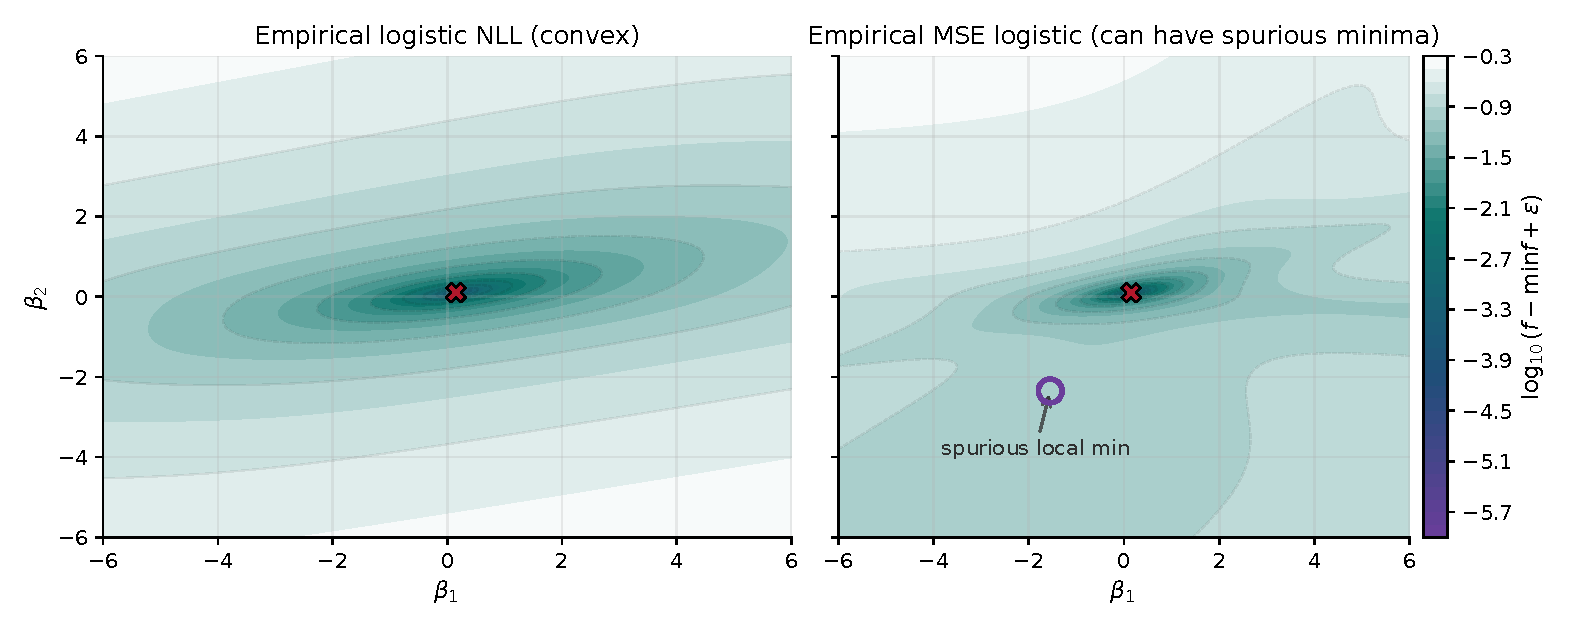
\includegraphics[width=\textwidth]{figures/handouts/convexity_optimization/fig_logistic_empirical_spurious}
  \caption{Empirical logistic landscapes on the dataset in \Cref{ex:logistic-empirical-spurious}.
  The plots show $\log_{10}(f-\min f+\varepsilon)$ for each objective.
  The red X marks the global minimizer in each panel.
  Left: the NLL is convex (one basin).
  Right: the squared-loss objective can have a spurious local minimum (circled), so a local method can get stuck.}
  \label{fig:logistic-empirical-spurious}
\end{figure}

\begin{figure}[t]
  \centering
  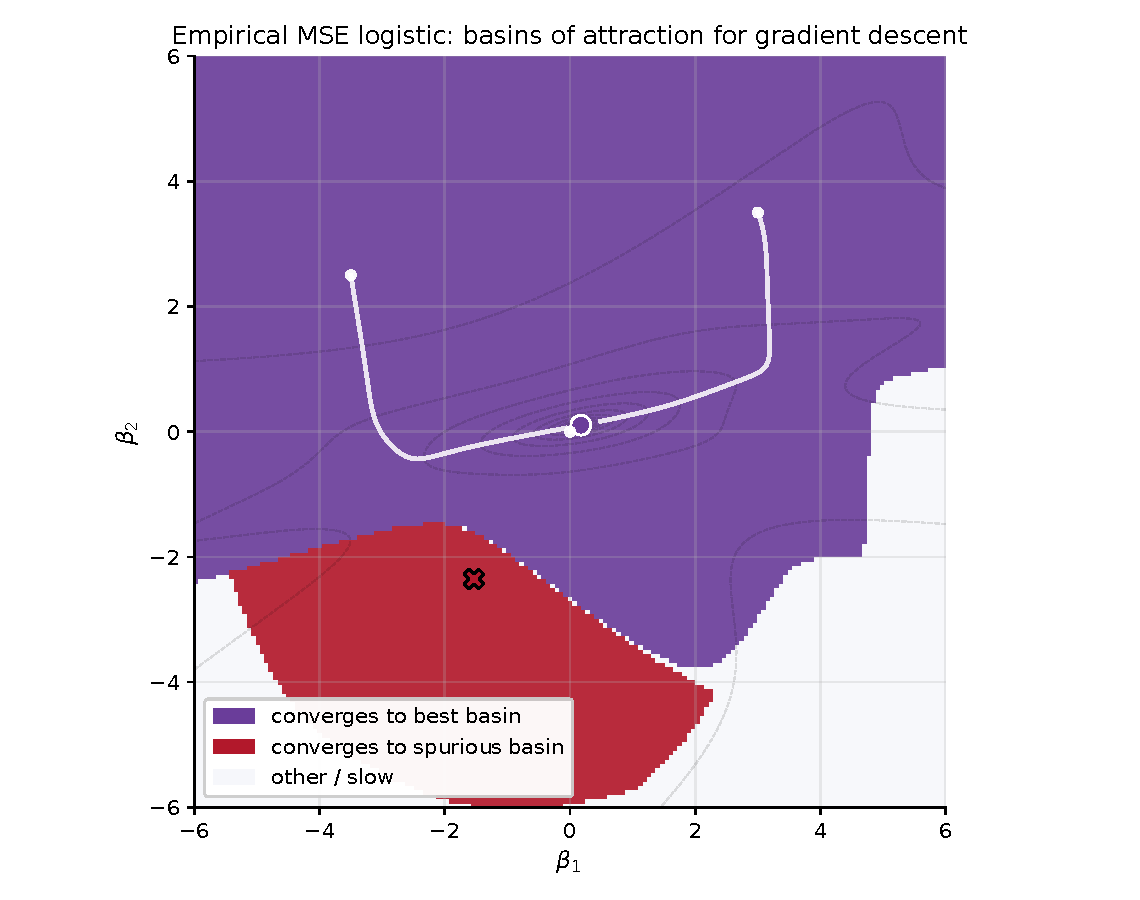
\includegraphics[width=0.92\textwidth]{figures/handouts/convexity_optimization/fig_logistic_empirical_basins}
  \caption{Basins of attraction for gradient descent on the empirical MSE-logistic objective in \Cref{ex:logistic-empirical-spurious}.
  The purple dot and red X mark the two local minimizers.
  Each initialization is colored by which local minimizer fixed-step GD (with $\eta=0.6$) converges to, and the overlaid paths show a few representative trajectories.}
  \label{fig:logistic-empirical-basins}
\end{figure}

Now assume a realizable population model:
\[
Y\mid X=x \sim \mathrm{Bernoulli}(p^\star(x)),
\qquad
p^\star(x) = \sigma(x^\top\beta^\star).
\]
Then the expected squared loss decomposes as
\[
\E\big[(Y-\sigma(X^\top\beta))^2\mid X\big]
= p^\star(X)(1-p^\star(X)) + \big(p^\star(X)-\sigma(X^\top\beta)\big)^2,
\]
so (up to an additive constant) the population objective becomes
\begin{equation}
R(\beta) = \E\big[(\sigma(X^\top\beta)-\sigma(X^\top\beta^\star))^2\big].
\label{eq:logistic-pop-risk}
\end{equation}

\begin{proposition}[One-point monotonicity in the realizable population squared-loss risk]
\label{prop:logistic-pop-one-point}
Assume $\E[\norm{X}_2]<\infty$, and let $R$ be as in \eqref{eq:logistic-pop-risk}. Then for all $\beta$,
\begin{equation}
\ip{\nabla R(\beta)}{\beta-\beta^\star} \ge 0.
\label{eq:one-point}
\end{equation}
In particular, along any ray $\beta(t)=\beta^\star+t(\beta-\beta^\star)$, the function $t\mapsto R(\beta(t))$ is nondecreasing for $t\ge 0$.
\end{proposition}

The next exercise isolates the population monotonicity calculation; structurally it plays the same role as the first-order convexity arguments in the Optimization unit.
\begin{exercise}[One-point monotonicity for realizable MSE-logistic]
\label{ex:logistic-one-point}
Prove \Cref{prop:logistic-pop-one-point}.
Let $\eta=X^\top\beta$ and $\eta^\star=X^\top\beta^\star$.
\begin{enumerate}[leftmargin=*]
  \item Differentiate under the expectation in \eqref{eq:logistic-pop-risk} to show that
  \[
  \nabla R(\beta)
  =2\,\E\Big[(\sigma(\eta)-\sigma(\eta^\star))\,\sigma'(\eta)\,X\Big].
  \]
  \item Show that
  \[
  \ip{\nabla R(\beta)}{\beta-\beta^\star}
  =2\,\E\Big[\sigma'(\eta)\,(\sigma(\eta)-\sigma(\eta^\star))(\eta-\eta^\star)\Big],
  \]
  and conclude it is nonnegative using only that $\sigma$ is increasing and $\sigma'\ge 0$.
  \item Deduce the ray-monotonicity statement by differentiating $g(t)=R(\beta^\star+t(\beta-\beta^\star))$.
\end{enumerate}
\end{exercise}

\SolutionBox[14]{%
\emph{Part (1).}
Differentiate \eqref{eq:logistic-pop-risk} under the expectation:
\[
R(\beta)=\E\big[(\sigma(X^\top\beta)-\sigma(X^\top\beta^\star))^2\big].
\]
Using the chain rule, $\nabla_\beta\sigma(X^\top\beta)=\sigma'(X^\top\beta)\,X$, hence
\[
\nabla R(\beta)
=2\,\E\Big[(\sigma(\eta)-\sigma(\eta^\star))\,\sigma'(\eta)\,X\Big],
\qquad
\eta=X^\top\beta,\ \eta^\star=X^\top\beta^\star.
\]

\emph{Part (2).}
Take the inner product with $(\beta-\beta^\star)$ and use $\ip{X}{\beta-\beta^\star}=\eta-\eta^\star$:
\[
\ip{\nabla R(\beta)}{\beta-\beta^\star}
=2\,\E\Big[\sigma'(\eta)\,(\sigma(\eta)-\sigma(\eta^\star))(\eta-\eta^\star)\Big].
\]
Since $\sigma'(\eta)\ge 0$ and $\sigma$ is increasing, we have
$(\sigma(\eta)-\sigma(\eta^\star))(\eta-\eta^\star)\ge 0$ pointwise.
Therefore the integrand is pointwise nonnegative, and the expectation is nonnegative as claimed.

\emph{Part (3) (ray monotonicity).}
For the ray $\beta(t)=\beta^\star+t(\beta-\beta^\star)$, define $g(t)=R(\beta(t))$.
By the chain rule,
\[
g'(t)=\ip{\nabla R(\beta(t))}{\beta-\beta^\star}\ge 0,
\]
so $t\mapsto R(\beta(t))$ is nondecreasing for $t\ge 0$.
(The argument uses only that the link is increasing with nonnegative derivative, so it holds for any such link function.)%
}

\begin{corollary}[Realizable population MSE-logistic has no spurious local minima]
\label{cor:logistic-pop-no-spurious}
Under the assumptions of \Cref{prop:logistic-pop-one-point}, every local minimizer of the realizable population risk $R$ in \eqref{eq:logistic-pop-risk} is global.
If in addition $\E[XX^\top]\succ 0$, then the unique global minimizer is $\beta^\star$.
\end{corollary}

\begin{exercise}[Stationarity + one-point monotonicity $\Rightarrow$ no spurious local minima]
\label{ex:logistic-one-point-no-spurious}
Prove \Cref{cor:logistic-pop-no-spurious} from \Cref{prop:logistic-pop-one-point}.
\begin{enumerate}[leftmargin=*]
  \item Let $\bar\beta$ be a local minimizer. Since $R$ is differentiable, $\nabla R(\bar\beta)=0$.
  Combine this with \Cref{eq:one-point} to show that
  \[
    0
    = \ip{\nabla R(\bar\beta)}{\bar\beta-\beta^\star}
    = 2\,\E\Big[\sigma'(\bar\eta)\,(\sigma(\bar\eta)-\sigma(\eta^\star))(\bar\eta-\eta^\star)\Big],
  \]
  where $\bar\eta=X^\top\bar\beta$ and $\eta^\star=X^\top\beta^\star$.
  Conclude that $\sigma(X^\top\bar\beta)=\sigma(X^\top\beta^\star)$ almost surely.
  \item Deduce that $R(\bar\beta)=0$, so $\bar\beta$ is a global minimizer.
  \item For uniqueness: show that if $R(\beta)=0$, then $X^\top(\beta-\beta^\star)=0$ almost surely, and deduce $\beta=\beta^\star$ under $\E[XX^\top]\succ 0$.
\end{enumerate}
\end{exercise}

\SolutionBox[14]{%
\emph{Part (1).}
Let $\bar\beta$ be a local minimizer of the differentiable function $R$.
Then $\nabla R(\bar\beta)=0$.
Applying \Cref{prop:logistic-pop-one-point} at $\beta=\bar\beta$ gives
\[
0
= \ip{\nabla R(\bar\beta)}{\bar\beta-\beta^\star}
= 2\,\E\Big[\sigma'(\bar\eta)\,(\sigma(\bar\eta)-\sigma(\eta^\star))(\bar\eta-\eta^\star)\Big],
\qquad \bar\eta=X^\top\bar\beta,\ \eta^\star=X^\top\beta^\star.
\]
The integrand is pointwise nonnegative because $\sigma'(\bar\eta)\ge 0$ and $\sigma$ is increasing, so the expectation can vanish only if the integrand is zero almost surely.
Since $\sigma'(z)>0$ for every finite $z$, this implies
\[
(\sigma(\bar\eta)-\sigma(\eta^\star))(\bar\eta-\eta^\star)=0
\qquad\text{almost surely.}
\]
Because $\sigma$ is strictly increasing, the product above is zero if and only if $\bar\eta=\eta^\star$, equivalently $\sigma(X^\top\bar\beta)=\sigma(X^\top\beta^\star)$ almost surely.

\emph{Part (2).}
If $\sigma(X^\top\bar\beta)=\sigma(X^\top\beta^\star)$ almost surely, then the integrand in \eqref{eq:logistic-pop-risk} vanishes almost surely, so
\[
R(\bar\beta)=\E\big[(\sigma(X^\top\bar\beta)-\sigma(X^\top\beta^\star))^2\big]=0.
\]
Since $R(\beta^\star)=0$ as well, $\bar\beta$ is a global minimizer.

\emph{Part (3) (uniqueness).}
If $R(\beta)=0$, then
\[
\E\big[(\sigma(X^\top\beta)-\sigma(X^\top\beta^\star))^2\big]=0,
\]
so $\sigma(X^\top\beta)=\sigma(X^\top\beta^\star)$ almost surely.
Since $\sigma$ is strictly increasing, this implies $X^\top(\beta-\beta^\star)=0$ almost surely.
Taking expectations yields
$(\beta-\beta^\star)^\top\E[XX^\top](\beta-\beta^\star)=0$.
If $\E[XX^\top]\succ 0$, then the quadratic form is strictly positive unless $\beta=\beta^\star$, so $\beta^\star$ is the unique global minimizer.%
}

The population MSE-logistic risk is nonconvex, but it still has the simple geometry that moving away from $\beta^\star$ does not help along any ray from $\beta^\star$.
This is qualitatively different from objectives like ecological logistic regression (\Cref{sec:ecological-logistic}), where aggregation introduces intrinsic nonconvexity and the landscape can have many distinct basins even under a clean population model.

Even with this benign global geometry, gradient descent can be slow because of saturation and flat plateaus.
The one-point monotonicity in \Cref{prop:logistic-pop-one-point} is a global geometry guarantee, but it is not a rate guarantee.
Far from $\beta^\star$, the squared-loss logistic objective can become very flat because the logistic link saturates:
$\sigma(z)\to 0$ or $1$ and $\sigma'(z)\to 0$ as $|z|\to\infty$.
The squared-loss gradient carries a factor of $\sigma'(X^\top\beta)$, so when the model is very confident (large $|X^\top\beta|$), the gradient can be tiny even if the objective value is not close to its minimum.
This mirrors the ``confidence weights'' story for convex NLL objectives:
in logistic NLL, curvature is largest near the decision boundary, while very confident points contribute little.
For squared loss, that same saturation suppresses the \emph{descent signal} itself, producing plateaus where $\norm{\nabla R(\beta)}_2$ is small even though $R(\beta)-R(\beta^\star)$ is not.

\begin{proposition}[Realizable squared-loss logistic: arbitrarily flat far from $\beta^\star$]
\label{prop:logistic-pop-flat}
Assume $\E[\norm{X}_2]<\infty$ and let $R$ be the realizable population risk \eqref{eq:logistic-pop-risk}.
Define $g(t)=R(t\beta^\star)$ for $t\ge 1$.
Then:
\begin{enumerate}[leftmargin=*]
  \item $g$ is nondecreasing on $[1,\infty)$ and converges to a finite limit $g(\infty)$.
  \item $\lim_{t\to\infty} g'(t)=0$ and $\lim_{t\to\infty}\norm{\nabla R(t\beta^\star)}_2=0$.
  \item If $\Pr(X^\top\beta^\star\neq 0)>0$, then $g(\infty)>0$.
\end{enumerate}
In particular, there are directions along which the landscape becomes arbitrarily flat even though the excess risk stays bounded away from $0$.
\end{proposition}

\emph{Proof idea.} See Exercise~\ref{ex:logistic-plateau}.

\begin{exercise}[Prove the plateau]
\label{ex:logistic-plateau}
In the realizable population model, let $g(t)=R(t\beta^\star)$ for $t\ge 1$.
\begin{enumerate}[leftmargin=*]
  \item Show that
  \[
    g'(t)=2\,\E\big[(\sigma(t\eta^\star)-\sigma(\eta^\star))\,\sigma'(t\eta^\star)\,\eta^\star\big],
    \qquad \eta^\star=X^\top\beta^\star,
  \]
  and conclude that $g$ is nondecreasing (hence $g(t)\to g(\infty)$ since $0\le g(t)\le 1$).
  \item Show that $g'(t)\to 0$ and $\nabla R(t\beta^\star)\to 0$ as $t\to\infty$.
  Interpret this as: \emph{without} a PL/strong-convexity-type condition, small gradient does not imply near-optimality.
  \item Assume $\Pr(\eta^\star\neq 0)>0$.
  Show that $g(\infty)>0$.
\end{enumerate}
\end{exercise}

\SolutionBox[12]{%
Write $\eta^\star=X^\top\beta^\star$ so that $g(t)=\E[(\sigma(t\eta^\star)-\sigma(\eta^\star))^2]$.

\emph{Part (1).}
Differentiate under the expectation:
by the chain rule,
\[
\frac{d}{dt}\sigma(t\eta^\star)=\sigma'(t\eta^\star)\,\eta^\star,
\]
so
\[
g'(t)
=\E\Big[2(\sigma(t\eta^\star)-\sigma(\eta^\star))\cdot \sigma'(t\eta^\star)\,\eta^\star\Big]
=2\,\E\big[(\sigma(t\eta^\star)-\sigma(\eta^\star))\,\sigma'(t\eta^\star)\,\eta^\star\big].
\]
For $t\ge 1$, $\sigma(t\eta^\star)-\sigma(\eta^\star)$ has the same sign as $(t-1)\eta^\star$ since $\sigma$ is increasing.
Because $\sigma'\ge 0$, the integrand is pointwise nonnegative, hence $g'(t)\ge 0$ and $g$ is nondecreasing.
Since $g(t)\in[0,1]$, it follows that $g(t)\to g(\infty)$ for some finite limit $g(\infty)$.

\emph{Part (2).}
For each fixed $\eta^\star\neq 0$, we have $t\eta^\star\to \pm\infty$ and therefore $\sigma'(t\eta^\star)\to 0$ as $t\to\infty$.
Also,
\[
\big|(\sigma(t\eta^\star)-\sigma(\eta^\star))\,\sigma'(t\eta^\star)\,\eta^\star\big|
\le \sigma'(0)\,|\eta^\star|
\le \sigma'(0)\,\norm{\beta^\star}_2\,\norm{X}_2,
\]
which is integrable since $\E[\norm{X}_2]<\infty$.
We will use the following standard fact: if random variables $Z_t$ satisfy $|Z_t|\le W$ with $\E[W]<\infty$ and $Z_t\to 0$ almost surely, then $\E[Z_t]\to 0$.
Applying this fact here gives $g'(t)\to 0$ as $t\to\infty$.

\smallskip
Similarly, differentiating \eqref{eq:logistic-pop-risk} gives
\[
\nabla R(t\beta^\star)
=2\,\E\big[(\sigma(t\eta^\star)-\sigma(\eta^\star))\,\sigma'(t\eta^\star)\,X\big].
\]
The integrand norm is bounded by $2\sigma'(0)\norm{X}_2$, and for each fixed $X$ the factor $\sigma'(t\eta^\star)$ tends to $0$ (or the bracketed term vanishes when $\eta^\star=0$), so the same reasoning lets us pass the limit through the expectation and conclude $\nabla R(t\beta^\star)\to 0$.

\emph{Part (3).}
As $t\to\infty$ we have $\sigma(t\eta^\star)\to 1$ when $\eta^\star>0$, $\sigma(t\eta^\star)\to 0$ when $\eta^\star<0$, and $\sigma(t\eta^\star)=\sigma(\eta^\star)=1/2$ when $\eta^\star=0$.
Since $0\le (\sigma(t\eta^\star)-\sigma(\eta^\star))^2\le 1$, we can apply the same fact (with $W=1$) to pass the limit through the expectation and obtain
\[
g(\infty)=\E\Big[(1-\sigma(\eta^\star))^2\mathbf{1}\{\eta^\star>0\} + \sigma(\eta^\star)^2\mathbf{1}\{\eta^\star<0\}\Big].
\]
If $\Pr(\eta^\star\neq 0)>0$, then the integrand is strictly positive on $\{\eta^\star\neq 0\}$, so $g(\infty)>0$.

Along this ray, the risk can remain bounded away from $0$ while the gradient (and directional derivative) goes to $0$.
Without a condition like PL/strong convexity, a small gradient does not by itself certify near-optimality.
}

Conditions like strong convexity or the PL inequality (\Cref{def:pl-inequality}) prevent this phenomenon: they rule out large flat regions away from the optimum by relating gradient size to suboptimality.
\Cref{prop:logistic-pop-flat} shows the realizable squared-loss logistic risk does not have such a global guarantee in general.

In the realizable population model, the one-point monotonicity in \Cref{prop:logistic-pop-one-point} is a \emph{global} geometric statement.
To get an actual rate for gradient descent, we also need a \emph{local curvature} condition near $\beta^\star$.
One simple sufficient condition is bounded features, which implies local strong convexity (hence a linear rate) around the optimum.

\begin{proposition}[Local linear convergence of gradient descent near $\beta^\star$]
\label{prop:logistic-pop-local-rate}
Assume $\E[XX^\top]\succeq \lambda I_d$ and $\norm{X}_2\le R$ almost surely for some $\lambda,R>0$.
Then at $\beta^\star$,
\[
\Hess R(\beta^\star)\succeq m_0 I_d,
\qquad
m_0 = 2\,\sigma'(R\norm{\beta^\star}_2)^2\,\lambda,
\]
and there exist $r>0$ and constants $0<m\le L<\infty$ such that the population risk $R$ in \eqref{eq:logistic-pop-risk} is $m$-strongly convex and $L$-smooth on the ball $\{\beta:\ \norm{\beta-\beta^\star}_2\le r\}$.
Consequently, gradient descent with step size $1/L$ initialized in this ball satisfies
\[
R(\beta^{(k)})-R(\beta^\star)
\le \left(1-\frac{m}{L}\right)^k\bigl(R(\beta^{(0)})-R(\beta^\star)\bigr)
\qquad\text{(see \citealp[\S9.3]{boyd_vandenberghe_2004_convex}).}
\]
\end{proposition}

\begin{proof}
Differentiate \eqref{eq:logistic-pop-risk} twice.
At $\beta=\beta^\star$, the cross term vanishes and the Hessian simplifies to
\[
\Hess R(\beta^\star)=2\,\E\big[\sigma'(X^\top\beta^\star)^2\,XX^\top\big].
\]
Since $\norm{X^\top\beta^\star}\le \norm{X}_2\norm{\beta^\star}_2\le R\norm{\beta^\star}_2$ almost surely, we have
$\sigma'(X^\top\beta^\star)\ge \sigma'(R\norm{\beta^\star}_2)>0$ almost surely (since $\sigma'$ is even and decreases with $|z|$), hence
\[
\Hess R(\beta^\star)\succeq 2\,\sigma'(R\norm{\beta^\star}_2)^2\,\E[XX^\top]\succeq 2\,\sigma'(R\norm{\beta^\star}_2)^2\,\lambda I_d.
\]
This is the claimed bound with $m_0=2\,\sigma'(R\norm{\beta^\star}_2)^2\,\lambda$.
Because $R$ is twice continuously differentiable and $\norm{X}_2\le R$ almost surely, $\Hess R(\beta)$ varies continuously in $\beta$ and is bounded on compact sets.
Therefore, on a sufficiently small ball around $\beta^\star$, the Hessian is bounded below by (say) $\tfrac12 m_0 I_d$ and above by $L I_d$ for some finite $L$, which gives local strong convexity and smoothness.
The linear convergence rate for gradient descent on an $m$-strongly convex and $L$-smooth function is standard (cited above).
\end{proof}

Under misspecification, hard multimodality can return.
If $p^\star(x)$ is not representable as $\sigma(x^\top\beta)$ (e.g.\ marginalizing over latent classes can yield mixtures of logits), then \eqref{eq:one-point} need not hold, and the population squared-loss risk can become bimodal with spurious local minima.
Benign global geometry often hinges on model and data assumptions.
This is one reason MLE (convex NLL) is often more stable than squared-loss fitting in logistic-type binary regression models.

\begin{example}[Misspecification can create a spurious local minimum for squared-loss logistic regression]
\label{ex:logistic-misspecified-spurious}
Consider a 1D feature $X$ that takes values $\{-2,-1,1,2\}$ with equal probability, and parameterize $\beta=(\beta_0,\beta_1)$ so that $q_\beta(x)=\sigma(\beta_0+\beta_1 x)$.
Let the true conditional probabilities be
\[
p^\star(-2)=0.49,\quad p^\star(-1)=0.87,\quad p^\star(1)=0.92,\quad p^\star(2)=0.36.
\]
This $p^\star$ is not representable as $q_\beta$, since it is not monotone in $x$.

For the population squared-loss risk $R_{\mathrm{MSE}}(\beta)=\E[(q_\beta(X)-p^\star(X))^2]$, a direct evaluation shows two distinct basins:
numerically, evaluating $R_{\mathrm{MSE}}$ on a grid reveals a global minimizer and a spurious local minimizer.
See \Cref{fig:logistic-landscape-2d}.
\end{example}

\begin{figure}[t]
  \centering
  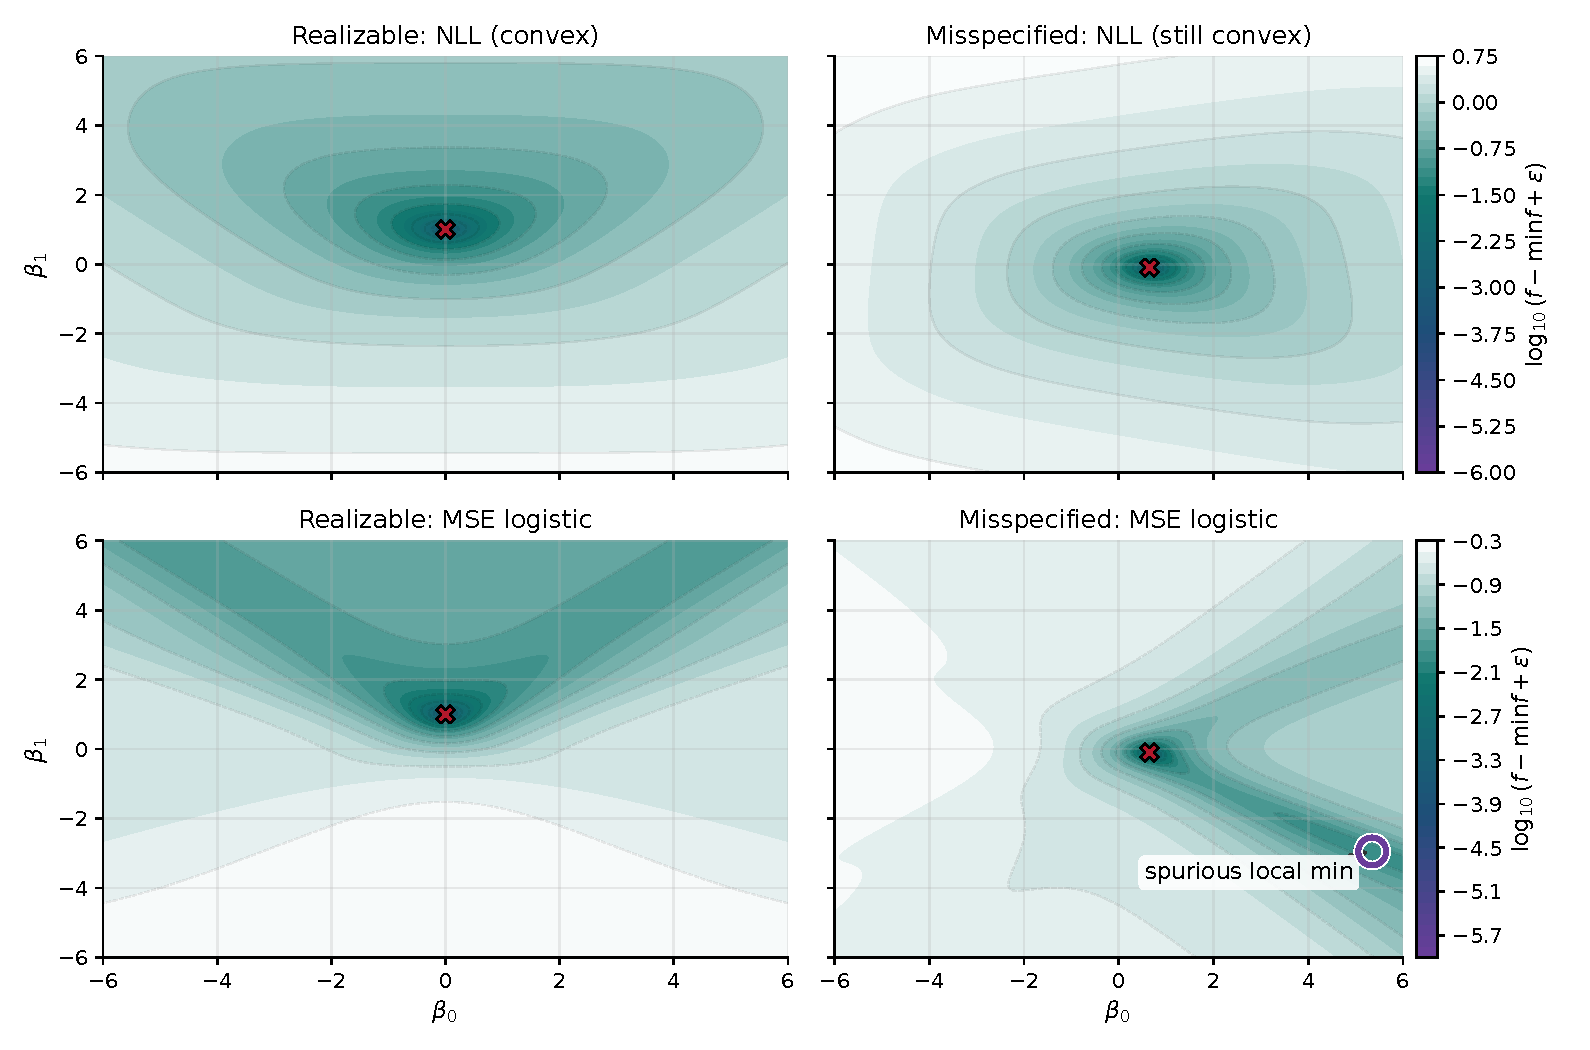
\includegraphics[width=\textwidth]{figures/handouts/convexity_optimization/fig_logistic_landscape_2d}
  \caption{A consistent contourf view of logistic landscapes in a 2D parameterization $\beta=(\beta_0,\beta_1)$.
  The plots show $\log_{10}(f-\min f+\varepsilon)$ for each objective, which makes basins comparable across panels.
  The red X marker indicates the global minimizer in each panel; in the bottom-right plot, the circled point is a spurious local minimum.
  In this example, the NLL landscape is unimodal in both realizable and misspecified settings, while the squared-loss landscape can develop extra basins under misspecification.}
  \label{fig:logistic-landscape-2d}
\end{figure}

% ------------------------------------------------------------
Example~I separates three distinct regimes.
Empirical MSE-logistic can create spurious basins; the realizable population risk has no spurious local minima but can still be slow because of broad plateaus; and misspecification can bring back genuinely wrong stable basins.
The response depends on the regime: use a stable objective when possible, use damping or line search when curvature is unreliable, and use restarts or stronger initializations when multiple basins are present.

% ------------------------------------------------------------
\section[Example II (phase retrieval)]{Example II: multimodality from symmetry, but only global optima in phase retrieval}
\label{sec:phase-retrieval}

In coherent diffraction imaging, optics, and astronomy, sensors measure intensities and lose phase.
A canonical real model is \emph{phase retrieval}:
\[
y_i = (a_i^\top x^\star)^2,\qquad i=1,\dots,m,
\]
where $x^\star\in\R^d$ is the unknown signal and $a_i$ are known sensing vectors.
A standard nonconvex least-squares objective is
\begin{equation}
F(x)=\frac{1}{4m}\sum_{i=1}^m\big((a_i^\top x)^2 - y_i\big)^2.
\label{eq:phase-empirical}
\end{equation}
This objective is nonconvex for structural reasons (it involves squares of linear forms),
and it is \emph{inherently} multimodal because $x^\star$ and $-x^\star$ generate the same data.

Like squared-loss logistic regression, phase retrieval is a smooth, nonconvex least-squares objective.
But here the nonconvexity is driven primarily by a \emph{symmetry}: $x^\star$ and $-x^\star$ generate the same data.
In population (for Gaussian designs), this symmetry produces multiple global optima but \emph{no} suboptimal local minima; the remaining stationary points are saddles.
This is ``benign'' nonconvexity (a strict-saddle picture), and it contrasts with ecological logistic regression (\Cref{sec:ecological-logistic}), where aggregation creates intrinsic nonconvexity and can lead to many distinct basins.
This ``benign geometry'' picture (multiple equivalent global minimizers; strict saddles elsewhere) appears broadly in modern tractable nonconvex problems; see \citet[\S2]{sun_qu_wright_2015_nonconvex_not_scary} and \citet[\S1]{zhang_qu_wright_2020_symmetry_geometry}.

\begin{figure}[t]
  \centering
  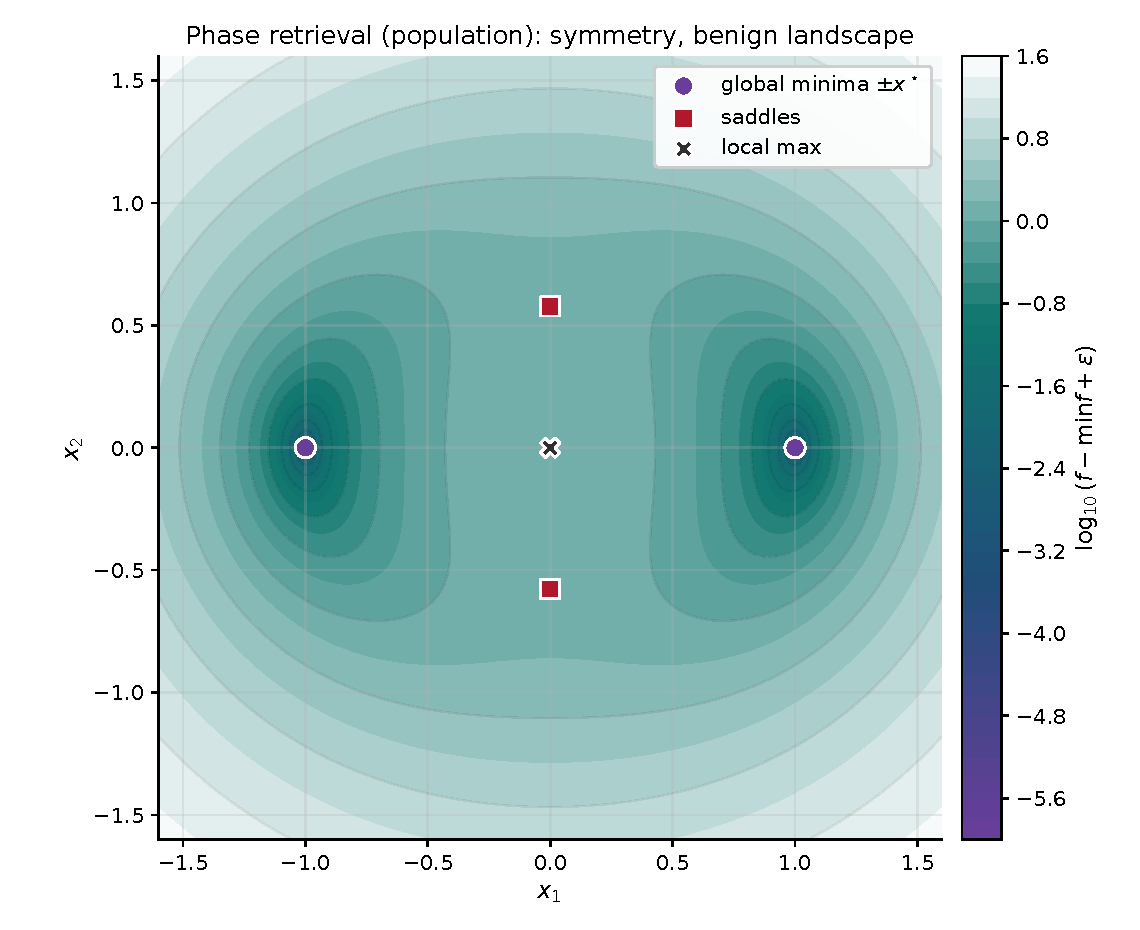
\includegraphics[width=0.86\textwidth]{figures/handouts/convexity_optimization/fig_phase_retrieval_landscape}
  \caption{Population phase retrieval in $d=2$: the landscape is nonconvex and symmetric ($x\sim -x$), but the only local minima are the two global minima $\pm x^\star$; other critical points are saddles or a local maximum at the origin.}
  \label{fig:phase-retrieval-landscape}
\end{figure}

For a clean population model, assume $a\sim N(0,I_d)$ and consider the \emph{population} objective
\begin{equation}
  f(x)=\frac12\,\E\Big[\big((a^\top x)^2 - (a^\top x^\star)^2\big)^2\Big].
  \label{eq:phase-pop}
\end{equation}

\begin{proposition}[Population phase retrieval: nonconvex but no spurious local minima]
\label{prop:phase-retrieval-benign}
For $f$ in \eqref{eq:phase-pop},
\begin{equation}
  f(x)
  =\frac{3}{2}\norm{x}^4 - \norm{x}^2\norm{x^\star}^2 - 2\ip{x}{x^\star}^2 + \frac{3}{2}\norm{x^\star}^4,
  \label{eq:phase-pop-closed-form}
\end{equation}
and the stationary points are:
\begin{enumerate}[leftmargin=*]
  \item global minima $x=\pm x^\star$ (value $0$),
  \item a local maximum at $x=0$,
  \item a saddle set $\{x:\ x\perp x^\star,\ \norm{x}=\norm{x^\star}/\sqrt{3}\}$.
\end{enumerate}
In particular, every local minimum is global.
\end{proposition}

\begin{exercise}[Phase retrieval: derive and classify the population stationary points]
\label{ex:phase-pop-derivation}
Prove \Cref{prop:phase-retrieval-benign}.
\begin{enumerate}[leftmargin=*]
  \item Expand \eqref{eq:phase-pop} and use the Gaussian fourth-moment identities
  \[
  \E[(a^\top u)^4]=3\norm{u}^4,
  \qquad
  \E[(a^\top u)^2(a^\top v)^2]=\norm{u}^2\norm{v}^2 + 2\ip{u}{v}^2,
  \]
  to obtain \eqref{eq:phase-pop-closed-form}.
  \item Differentiate \eqref{eq:phase-pop-closed-form} to get an explicit formula for $\nabla f(x)$.
  \item Solve $\nabla f(x)=0$ by decomposing $x=\alpha x^\star + u$ with $u\perp x^\star$.
  \item Classify the stationary points as global minima, a local maximum, and a saddle set.
\end{enumerate}
\end{exercise}

\SolutionBox[22]{%
\emph{Part (1) (closed form).}
Expanding the square in \eqref{eq:phase-pop} gives
\[
f(x)
=\frac12\,\E\big[(a^\top x)^4\big]
\;-\;\E\big[(a^\top x)^2(a^\top x^\star)^2\big]
\;+\;\frac12\,\E\big[(a^\top x^\star)^4\big].
\]
Apply the stated Gaussian fourth-moment identities with $u=x$ and $v=x^\star$ to get
\[
\E[(a^\top x)^4]=3\norm{x}^4,\qquad
\E[(a^\top x^\star)^4]=3\norm{x^\star}^4,
\]
and
\[
\E[(a^\top x)^2(a^\top x^\star)^2]=\norm{x}^2\norm{x^\star}^2 + 2\ip{x}{x^\star}^2.
\]
Substituting yields \eqref{eq:phase-pop-closed-form}.

\emph{Part (2) (gradient).}
Differentiate \eqref{eq:phase-pop-closed-form}:
\[
\nabla f(x)
= 6\norm{x}^2 x - 2\norm{x^\star}^2 x - 4\ip{x}{x^\star}x^\star
= (6\norm{x}^2-2\norm{x^\star}^2)x - 4\ip{x}{x^\star}x^\star.
\]

\emph{Part (3) (stationary points).}
Let $r=\norm{x^\star}_2$ and decompose $x=\alpha x^\star + u$ with $u\perp x^\star$.
Then $\ip{x}{x^\star}=\alpha r^2$ and $\norm{x}^2=\alpha^2r^2+\norm{u}^2$.
Setting $\nabla f(x)=0$ and matching the $u$ and $x^\star$ components gives
\[
(6\norm{x}^2-2r^2)\,u=0,
\qquad
\alpha\,(6\norm{x}^2-6r^2)=0.
\]
If $u=0$, then either $\alpha=0$ (so $x=0$) or $\norm{x}^2=r^2$ (so $\alpha=\pm 1$ and $x=\pm x^\star$).
If $u\neq 0$, then the first equation forces $\norm{x}^2=r^2/3$, and the second forces $\alpha=0$, hence
$x\perp x^\star$ and $\norm{x}=r/\sqrt{3}$.
This gives exactly the stationary-point list in \Cref{prop:phase-retrieval-benign}.

\emph{Part (4) (classification).}
Since $f$ in \eqref{eq:phase-pop} is an expectation of a square, $f(x)\ge 0$ for all $x$.
Also $f(\pm x^\star)=0$, so $\pm x^\star$ are global minima.

For $x=0$, the expansion \eqref{eq:phase-pop-closed-form} shows
\[
f(0)-f(x)= r^2\norm{x}^2 + 2\ip{x}{x^\star}^2 - \frac{3}{2}\norm{x}^4,
\]
which is strictly positive for all sufficiently small $x\neq 0$ (the quadratic term dominates), so $x=0$ is a local maximum.

Finally, if $x\perp x^\star$ and $\norm{x}=r/\sqrt{3}$, then the univariate restriction $t\mapsto f(x+t x^\star)$ has negative second derivative at $t=0$, so there is a direction of negative curvature.
Hence these points are saddles, and every local minimum is global.%
}

This is symmetry-driven nonconvexity with a strict-saddle geometry:
every non-optimal stationary point has a direction of negative curvature.

Phase retrieval is typically approached via the two-stage template in \Cref{alg:two-stage-template}:
use a cheap global initializer, then run a local method.
In the Gaussian model, there is a clean way to build a provably good direction estimate from a simple moment identity.
Assume the noiseless Gaussian design model $a_i \stackrel{\mathrm{iid}}{\sim} N(0,I_d)$ with measurements $y_i=(a_i^\top x^\star)^2$.
Define the \emph{spectral matrix}
\[
  Y = \frac{1}{m}\sum_{i=1}^m y_i a_i a_i^\top.
\]
Also define the radius estimate
\[
  \hat r^2 = \frac{1}{m}\sum_{i=1}^m y_i,
\]
which satisfies $\E[\hat r^2]=\norm{x^\star}_2^2$.
If $\hat u$ is a unit-norm top eigenvector of $Y$, then the standard spectral initializer is $x^{(0)}=\hat r\,\hat u$.

The next proposition explains why this initialization is reasonable.
It shows that (i) the population matrix $\E[Y]$ has a unique leading eigenvector in the $x^\star$ direction, and (ii) if the empirical $Y$ is close to $\E[Y]$ in operator norm then its leading eigenvector must be close to $\pm x^\star/\norm{x^\star}_2$.
(Here $\norm{M}_{\mathrm{op}}$ denotes the operator norm, i.e.\ the largest absolute eigenvalue for a symmetric matrix $M$.)

\begin{proposition}[Gaussian phase retrieval: why the spectral initializer points at $x^\star$]
\label{prop:phase-spectral-init}
Assume $x^\star\neq 0$, let $a\sim N(0,I_d)$, and set $y=(a^\top x^\star)^2$.
Write $r=\norm{x^\star}_2$ and $u^\star=x^\star/r$.
Define the population matrix
\[
  Y_{\mathrm{pop}} = \E\big[y\,a a^\top\big]
  = \E\big[(a^\top x^\star)^2 a a^\top\big].
\]
Then
\[
  Y_{\mathrm{pop}}=r^2 I_d + 2x^\star(x^\star)^\top,
\]
so the unique leading eigenvector of $Y_{\mathrm{pop}}$ is $u^\star$.
Moreover, if $Y$ is any symmetric matrix satisfying
\[
\norm{Y-Y_{\mathrm{pop}}}_{\mathrm{op}} \le \varepsilon\, r^2
\qquad\text{for some }\varepsilon\in(0,1),
\]
then for every unit-norm leading eigenvector $\hat u$ of $Y$ there exists a sign $s\in\{\pm 1\}$ such that
$\norm{\hat u-su^\star}_2\le \sqrt{2\varepsilon}$.
\end{proposition}

\begin{exercise}[Phase retrieval: why spectral initialization points at $x^\star$]
\label{ex:phase-spectral-spike}
Prove \Cref{prop:phase-spectral-init}.
Conclude that if the empirical matrix $Y$ is close to $Y_{\mathrm{pop}}$ in operator norm, then its top eigenvector is close to $\pm u^\star$ and the spectral initializer $x^{(0)}=\hat r\,\hat u$ is close to $\pm x^\star$.
\emph{Hint:} to compute $Y_{\mathrm{pop}}$, you can either compute entries using the Gaussian fourth-moment identity
$\E[a_i a_j a_k a_\ell]=\delta_{ij}\delta_{k\ell}+\delta_{ik}\delta_{j\ell}+\delta_{i\ell}\delta_{jk}$,
or compute the entries directly by expanding.
For the perturbation bound, compare quadratic forms $v^\top Y v$ and use $|v^\top (Y-Y_{\mathrm{pop}}) v|\le \norm{Y-Y_{\mathrm{pop}}}_{\mathrm{op}}$ for unit $v$.
Finally, explain in a sentence why one expects $\norm{Y-Y_{\mathrm{pop}}}_{\mathrm{op}}$ to be small when $m$ is large in the Gaussian model.
\end{exercise}

\SolutionBox[20]{%
Write $u=x^\star$ and expand $y=(a^\top u)^2=\sum_{k,\ell} u_k u_\ell a_k a_\ell$.
For each entry $(i,j)$,
\[
\E\!\big[y\,a_i a_j\big]
=\sum_{k,\ell} u_k u_\ell\,\E[a_i a_j a_k a_\ell]
=\sum_{k,\ell} u_k u_\ell\bigl(\delta_{ij}\delta_{k\ell}+\delta_{ik}\delta_{j\ell}+\delta_{i\ell}\delta_{jk}\bigr).
\]
The first term gives $\delta_{ij}\sum_k u_k^2=\delta_{ij}\norm{u}_2^2$.
The second and third terms each give $u_i u_j$.
Thus $\E[y\,a_i a_j]=\norm{u}_2^2\,\delta_{ij}+2u_i u_j$, i.e.
$Y_{\mathrm{pop}}=\norm{u}_2^2 I_d + 2uu^\top$.

For eigenvalues, note that $Y_{\mathrm{pop}}u=(\norm{u}_2^2+2\norm{u}_2^2)u=3\norm{u}_2^2 u$.
If $w\perp u$, then $uu^\top w=0$ so $Y_{\mathrm{pop}}w=\norm{u}_2^2 w$.
Hence the unique top eigenspace is $\mathrm{span}\{u\}$.

Let $r=\norm{u}_2$ and $u^\star=u/r$.
Let $\hat u$ be a unit top eigenvector of $Y$.
Write $E=Y-Y_{\mathrm{pop}}$ and assume $\norm{E}_{\mathrm{op}}\le \varepsilon r^2$.
Then
\[
\hat u^\top Y_{\mathrm{pop}} \hat u
= \hat u^\top Y \hat u - \hat u^\top E \hat u
\ge \lambda_{\max}(Y) - \norm{E}_{\mathrm{op}}
\ge (u^\star)^\top Y u^\star - \norm{E}_{\mathrm{op}}
\ge 3r^2 - 2\varepsilon r^2.
\]
On the other hand,
$
\hat u^\top Y_{\mathrm{pop}} \hat u
= r^2 + 2r^2\,|\ip{\hat u}{u^\star}|^2.
$
Combining gives $|\ip{\hat u}{u^\star}|^2\ge 1-\varepsilon$.
Choosing the sign that maximizes the inner product,
\[
\min\{\norm{\hat u-u^\star}_2,\norm{\hat u+u^\star}_2\}^2
=2\bigl(1-|\ip{\hat u}{u^\star}|\bigr)
\le 2\bigl(1-|\ip{\hat u}{u^\star}|^2\bigr)
\le 2\varepsilon.
\]

The matrix $Y$ is an empirical average of i.i.d.\ symmetric matrices with mean $Y_{\mathrm{pop}}$.
To make this quantitative in high dimensions, one uses concentration inequalities for random matrices to bound $\norm{Y-Y_{\mathrm{pop}}}_{\mathrm{op}}$ with high probability; see \citet[\S2.2]{zhang_qu_wright_2020_symmetry_geometry} for discussion and references.
These probability tools are largely orthogonal to our focus here.%
}

Once you have an initialization that is close to $\pm x^\star$, the local stage behaves like the convex story again.
In the Gaussian population objective, $\pm x^\star$ are not only global minima: they are \emph{locally strongly convex} minima, so the standard local strong-convexity analysis from the Optimization unit gives a linear rate while the iterates remain in that neighborhood.

\begin{exercise}[Phase retrieval: local convexity near $\pm x^\star$ in the population objective]
\label{ex:phase-pop-local-strong-convex}
For the population objective $f$ in \eqref{eq:phase-pop-closed-form}, compute the Hessian $\Hess f(x)$ and show that
\[
\Hess f(x^\star)=4\norm{x^\star}_2^2 I_d + 8x^\star(x^\star)^\top.
\]
Deduce the eigenvalues of $\Hess f(x^\star)$ and interpret this as a local condition-number statement near $x^\star$.
\end{exercise}

\SolutionBox[12]{%
Differentiate the gradient formula in the solution to \Cref{ex:phase-pop-derivation}:
for $x\in\R^d$,
\[
\Hess f(x)=12xx^\top + (6\norm{x}_2^2-2\norm{x^\star}_2^2)I_d - 4x^\star(x^\star)^\top.
\]
At $x=x^\star$ this becomes
\[
\Hess f(x^\star)=(12-4)x^\star(x^\star)^\top + 4\norm{x^\star}_2^2 I_d
=8x^\star(x^\star)^\top + 4\norm{x^\star}_2^2 I_d.
\]
Along $u^\star=x^\star/\norm{x^\star}_2$ the eigenvalue is $12\norm{x^\star}_2^2$, and along any direction orthogonal to $x^\star$ the eigenvalue is $4\norm{x^\star}_2^2$.
So near $x^\star$ the population objective is well conditioned (local condition number $3$), which is exactly the regime where local methods behave like in the convex case.%
}

These pieces give the standard Gaussian-model story:
spectral initialization supplies a direction close to $\pm x^\star$, and the local geometry near $\pm x^\star$ is strongly convex, so local methods converge quickly once initialized there.
Rigorous finite-sample analyses follow this template; see \citet[\S2.2]{zhang_qu_wright_2020_symmetry_geometry} and references therein.

Phase retrieval shows a different kind of nonconvexity.
The sign symmetry creates multiple optima, but they are equivalent, and the remaining stationary points are saddles rather than bad local minima.
The right response is therefore not exhaustive global search; it is a coarse initializer, such as a spectral method, followed by local refinement inside the basin of $\pm x^\star$.



% ------------------------------------------------------------
\section[Example III (ecological logistic)]{Example III: hard nonconvexity from aggregation in ecological logistic regression}
\label{sec:ecological-logistic}

In some applications we observe covariates at the unit level but only aggregated outcomes.
For example, we might see covariates $x_{g,1},\dots,x_{g,n_g}$ for individuals in a group (a precinct, a cohort, a batch),
but instead of observing the binary outcomes $Y_{g,i}\in\{0,1\}$ we only observe the group total
\[
Z_g = \sum_{i=1}^{n_g} Y_{g,i}.
\]
Many different binary vectors $(Y_{g,1},\dots,Y_{g,n_g})$ can produce the same total $Z_g$, so the likelihood for $\beta$ must marginalize over a large discrete set of latent ``assignments.''

Assume a logistic model at the unit level:
\[
\Pr(Y_{g,i}=1\mid x_{g,i},\beta)=\sigma(x_{g,i}^\top\beta),
\qquad i=1,\dots,n_g,
\]
with conditional independence across $i$ given the covariates.
Write $p_{g,i}(\beta)=\sigma(x_{g,i}^\top\beta)$.
Then $Z_g$ is a sum of independent but non-identically distributed Bernoulli random variables (a Poisson--binomial model), and the marginal likelihood contains $\binom{n_g}{z_g}$ terms.
The resulting negative log-likelihood is typically nonconvex in $\beta$.
This combinatorial marginalization also creates a separate difficulty that is easy to miss if we focus only on the geometry:
when $n_g$ is large, the likelihood term $\Pr(Z_g=z_g\mid x_{g,1},\dots,x_{g,n_g},\beta)$ can be expensive to evaluate repeatedly inside an optimizer.
The naive computation is literally a sum over $\binom{n_g}{z_g}$ assignments (as in \Cref{ex:eco-logistic-nonconvex}), which is intractable for large groups.
This ``optimization + marginalization'' pattern is common in latent-variable models: hard landscapes and expensive objective evaluations can come together.

An empirical negative log-likelihood objective for $G$ independent groups is
\begin{equation}
  f(\beta)
  =
  -\frac{1}{G}\sum_{g=1}^G \log \Pr(Z_g=z_g \mid x_{g,1},\dots,x_{g,n_g},\beta).
  \label{eq:eco-logistic-obj}
\end{equation}
Two edge cases are instructive.
In the special case where the covariates are constant within each group ($x_{g,i}\equiv x_g$), we have
$Z_g\sim \mathrm{Binomial}(n_g,\sigma(x_g^\top\beta))$, and \eqref{eq:eco-logistic-obj} reduces to the usual convex binomial logistic-regression objective from the Optimization unit.
At the other extreme, if $d=1$ with $\beta=(\beta_0,\beta_1)$ and each group contains covariates in $\pm$ pairs (for every $x$ the value $-x$ appears with the same multiplicity), then the marginal likelihood is symmetric in the slope: it is unchanged under $\beta_1\mapsto -\beta_1$.
This kind of symmetry reflects a genuine non-identifiability from totals alone.

\begin{exercise}[Ecological logistic regression: two easy special cases]
\label{ex:eco-logistic-edge-cases}
\begin{enumerate}[leftmargin=*]
  \item Suppose $x_{g,i}\equiv x_g$ within each group.
  Show that $Z_g\sim \mathrm{Binomial}(n_g,\sigma(x_g^\top\beta))$ and conclude that the corresponding negative log-likelihood is convex in $\beta$.
  \item Assume $d=1$ with $\beta=(\beta_0,\beta_1)$ and suppose the multiset $\{x_1,\dots,x_n\}$ is symmetric: for every $x$ it contains $-x$ with the same multiplicity.
  Show that, for every $z$,
  \[
    \Pr(Z=z\mid x_1,\dots,x_n,(\beta_0,\beta_1))
    =
    \Pr(Z=z\mid x_1,\dots,x_n,(\beta_0,-\beta_1)).
  \]
  Conclude that the likelihood for $\beta_1$ is an even function, so the sign of the slope is not identifiable from $Z$ alone in such a balanced design.
\end{enumerate}
\end{exercise}

\SolutionBox[14]{%
\emph{Part (1).}
If $x_{g,i}\equiv x_g$, then conditional on $x_g$ the unit-level outcomes are i.i.d.\ Bernoulli with success probability $\sigma(x_g^\top\beta)$.
Therefore $Z_g=\sum_{i=1}^{n_g}Y_{g,i}\sim \mathrm{Binomial}(n_g,\sigma(x_g^\top\beta))$.
Up to an additive constant (independent of $\beta$), the per-group negative log-likelihood can be written as a function of the scalar $\eta=x_g^\top\beta$:
\[
\ell_g(\beta)
= -z_g\,\eta + n_g\log(1+e^\eta).
\]
Since $\frac{d^2}{d\eta^2}\ell_g(\eta)=n_g\,\sigma'(\eta)\ge 0$, the map $\eta\mapsto \ell_g(\eta)$ is convex.
Composing a convex function with a linear map $\beta\mapsto x_g^\top\beta$ preserves convexity, so $\ell_g$ is convex in $\beta$.
Summing over $g$ preserves convexity, hence the full objective is convex.

\emph{Part (2).}
Write $p_i(\beta_0,\beta_1)=\sigma(\beta_0+\beta_1 x_i)$.
Replacing $\beta_1$ by $-\beta_1$ replaces $p_i$ by $\tilde p_i=\sigma(\beta_0-\beta_1 x_i)$.
By the assumed symmetry of the multiset $\{x_i\}$, the multiset $\{\tilde p_i\}$ is the same as $\{p_i\}$ up to a permutation (each $x$ is paired with $-x$).
But the distribution of $Z=\sum_i Y_i$ depends only on the multiset of success probabilities, not on how they are ordered, so $\Pr(Z=z\mid x_1,\dots,x_n,(\beta_0,\beta_1))=\Pr(Z=z\mid x_1,\dots,x_n,(\beta_0,-\beta_1))$ for every $z$.
Thus the likelihood is an even function of $\beta_1$, which means the sign of the slope is not identifiable from totals in this balanced design.%
}

This example ties directly to the empirical-versus-population theme from Example~I.
There the bad basins can be a finite-sample artifact under benign population geometry; here the nonconvexity is intrinsic, because even under the correct model and infinite data aggregation forces us to marginalize over discrete latent assignments.
That marginalization step is also the bridge to the Expectation--maximization subsection of the Augmented-state optimization unit: once the assignments are latent, the natural algorithmic object is the EM update map, which alternates exact conditional expectations with parameter updates, rather than a single closed-form convex objective.

To emphasize this, it is useful to look at a \emph{population} version of \eqref{eq:eco-logistic-obj}.
Let $X=(x_1,\dots,x_n)$ denote a random group of covariates and let $Z$ be generated from the model under a true parameter $\beta^\star$.
Define the population objective
\[
F(\beta)=\E\big[-\log \Pr(Z\mid X,\beta)\big].
\]
Because the model is correctly specified, $F$ is minimized at (an observationally equivalent version of) $\beta^\star$.
However, as \Cref{fig:eco-logistic-pop-landscape} illustrates, $F$ can still have multiple separated basins and spurious local minima.

\begin{figure}[H]
  \centering
  \begin{tikzpicture}
  \pgfplotsset{table/search path={figures/handouts/convexity_optimization/,../../figures/handouts/convexity_optimization/,Lecture Tex/figures/handouts/convexity_optimization/}}

  \begin{axis}[
    width=0.88\linewidth,
    height=6.6cm,
    view={0}{90},
    axis lines=left,
    xlabel={$\beta_0$},
    ylabel={$\beta_1$},
    tick style={stat221Gray},
    tick label style={font=\small},
    label style={font=\small},
    xmin=-1.0, xmax=3.5,
    ymin=-2.0, ymax=2.0,
    point meta min=-4,
    point meta max=0.75,
    colormap={stat221landscape}{
      color=(stat221Purple)
      color=(stat221Blue)
      color=(stat221Teal)
      color=(white)
    },
    colorbar,
    colorbar style={
      ylabel={$\log_{10}(F-\min F+\varepsilon)$},
      width=0.32cm,
      yticklabel style={font=\small},
      ylabel style={font=\small},
      tick style={stat221Gray},
    },
  ]
    \addplot3[
      surf,
      shader=interp,
      mesh/rows=81,
      draw=none,
    ]
    table [x=beta0, y=beta1, z=loggap] {data_ecological_logistic_population_landscape.dat};

    % True parameter beta^*.
    \addplot3[only marks,mark=x,mark size=4.2,very thick,color=white] coordinates {(0.3,1.2,0.75)};
    \addplot3[only marks,mark=x,mark size=3.6,very thick,color=stat221Red] coordinates {(0.3,1.2,0.75)};

    % A few spurious local minima (approximate locations; shown as open circles).
    \addplot3[only marks,mark=o,mark size=4.0,very thick,color=white,fill=none] coordinates {(2.2,-1.05,0.75) (2.5,-1.15,0.75) (2.7,-1.25,0.75)};
    \addplot3[only marks,mark=o,mark size=3.4,very thick,color=stat221Gray,fill=none] coordinates {(2.2,-1.05,0.75) (2.5,-1.15,0.75) (2.7,-1.25,0.75)};
  \end{axis}
\end{tikzpicture}

  \caption{A toy \emph{population} objective for ecological logistic regression in a 2D parameterization $\beta=(\beta_0,\beta_1)$.
  Each group has $n=6$ units and is equally likely to have covariates $(-4,-3,-2,2,3,4)$, $(-3,-1,1,2,3,4)$, or $(-2,-1,1,2,3,4)$ (in $d=1$); outcomes are generated under $\beta^\star=(0.3,1.2)$.
  The plot shows $\log_{10}(F-\min F+\varepsilon)$, as in \Cref{fig:logistic-landscape-2d}; the red X marks $\beta^\star$ and the open circles mark three spurious local minima in this toy example.}
  \label{fig:eco-logistic-pop-landscape}
\end{figure}

\begin{exercise}[Ecological logistic regression: marginalization and nonconvexity]
\label{ex:eco-logistic-nonconvex}
Fix one group with covariates $x_1,\dots,x_n\in\R^d$ and observe $Z=z$.
Let $p_i(\beta)=\sigma(x_i^\top\beta)$.
\begin{enumerate}[leftmargin=*]
  \item Show that
  \[
    \Pr(Z=z\mid x_1,\dots,x_n,\beta)
    =
    \sum_{\substack{S\subseteq\{1,\dots,n\}\\|S|=z}}
    \ \prod_{i\in S} p_i(\beta)\prod_{j\notin S}\bigl(1-p_j(\beta)\bigr).
  \]
  Interpret this as summing over all ways to choose which $z$ units are the successes.
  \item Specialize to $n=2$ and $z=1$ in $d=1$ with covariates $x_1=a$ and $x_2=b$.
  Let $\ell(\beta)$ be the negative log-likelihood $-\log \Pr(Z=1\mid a,b,\beta)$ with no regularization.
  Show that $\ell''(0)=\tfrac12 ab$.
  Conclude that $\ell$ is not convex whenever $ab<0$.
\end{enumerate}
\end{exercise}

\SolutionBox[20]{%
\emph{Part (1).}
Condition on the covariates.
For any binary vector $y=(y_1,\dots,y_n)\in\{0,1\}^n$, conditional independence gives
\[
\Pr(Y_1=y_1,\dots,Y_n=y_n\mid x_1,\dots,x_n,\beta)
=
\prod_{i=1}^n p_i(\beta)^{y_i}\bigl(1-p_i(\beta)\bigr)^{1-y_i}.
\]
The event $\{Z=z\}$ is the union of all assignments $y$ with exactly $z$ ones, so summing over those assignments yields
\[
\Pr(Z=z\mid x_1,\dots,x_n,\beta)
=
\sum_{\substack{y\in\{0,1\}^n\\ \sum_i y_i=z}}
\ \prod_{i=1}^n p_i(\beta)^{y_i}\bigl(1-p_i(\beta)\bigr)^{1-y_i}.
\]
Reindexing the sum by the subset $S=\{i:\ y_i=1\}$ (which has $|S|=z$) gives the stated formula.

\emph{Part (2).}
For $n=2$ and $z=1$, let $p_1(\beta)=\sigma(a\beta)$ and $p_2(\beta)=\sigma(b\beta)$.
Then
\[
q(\beta)=\Pr(Z=1\mid a,b,\beta)
 = p_1(1-p_2) + (1-p_1)p_2
 = p_1+p_2-2p_1p_2,
\]
and $\ell(\beta)=-\log q(\beta)$.
At $\beta=0$ we have $p_1=p_2=\tfrac12$, so $q(0)=\tfrac12$.
Also $p_1'(\beta)=a\,p_1(1-p_1)$ and $p_2'(\beta)=b\,p_2(1-p_2)$, so $p_1'(0)=a/4$ and $p_2'(0)=b/4$.
A direct differentiation gives $q'(0)=0$ and
\[
q''(0)=-4p_1'(0)p_2'(0)=-4\cdot\frac{a}{4}\cdot\frac{b}{4}=-\frac{ab}{4}.
\]
Since $\ell'=-q'/q$ and $q'(0)=0$, we have $\ell''(0)=-(q''(0)/q(0))$ and therefore
\[
\ell''(0)
=-\frac{q''(0)}{q(0)}
=-\frac{-ab/4}{1/2}
=\frac{ab}{2}.
\]
If $ab<0$, then $\ell''(0)<0$, so $\ell$ is not convex.
}

Even though the landscape can be globally hard (and even the population objective can have spurious basins, as in \Cref{fig:eco-logistic-pop-landscape}), there is still a familiar ``convex'' story \emph{locally} around the true parameter under correct specification.
When the model is locally identifiable, the population objective has a neighborhood of $\beta^\star$ on which it is convex (indeed strongly convex).
One convenient way to see this in ecological logistic regression is to expose the probabilistic structure behind the gradient and Hessian: the observed-data objective involves marginalizing over latent assignments, and its Hessian can be written as a difference of two covariance matrices.
After averaging over the random total $Z$ under the true model, that difference becomes a covariance by the law of total covariance.

\begin{exercise}[Ecological logistic regression: DC structure and local convexity near $\beta^\star$]
\label{ex:eco-logistic-pop-local-convex}
Fix covariates $x_1,\dots,x_n\in\R^d$.
For $\beta\in\R^d$, let $V_1,\dots,V_n$ be independent Bernoulli random variables with
\[
\Pr(V_j=1\mid x_j,\beta)=\sigma(x_j^\top\beta),
\qquad j=1,\dots,n,
\]
and define
\[
U = \sum_{j=1}^n x_j V_j,
\qquad
Z = \sum_{j=1}^n V_j.
\]
For an observed total $Z=z$, write $L_z(\beta)=-\log \Pr(Z=z\mid x_1,\dots,x_n,\beta)$.
\begin{enumerate}[leftmargin=*]
  \item Show the \emph{difference-of-convex (DC)} form
  \[
  L_z(\beta)
  =\sum_{j=1}^n \log\bigl(1+e^{x_j^\top\beta}\bigr)
  -\log\left(\sum_{\substack{S\subseteq\{1,\dots,n\}\\|S|=z}} \exp\Big(\sum_{j\in S} x_j^\top\beta\Big)\right).
  \]
  \item Show that $\nabla L_z(\beta)=\E[U]-\E[U\mid Z=z]$.
  \item Show that $\Hess L_z(\beta)=\mathrm{Cov}(U)-\mathrm{Cov}(U\mid Z=z)$.
  (Hint: for $g(\beta)=\log\sum_k e^{a_k^\top\beta}$, the Hessian is the covariance of the vectors $\{a_k\}$ under the corresponding softmax weights.)
  \item Consider the population objective $F(\beta)=\E[L_Z(\beta)]$ when $Z$ is generated under a true parameter $\beta^\star$.
  Assuming the outer expectation defining $F$ can be differentiated twice under the integral sign, use the conditional law of total covariance,
  \[
    \mathrm{Cov}(U\mid X)=\E[\mathrm{Cov}(U\mid Z,X)\mid X] + \mathrm{Cov}(\E[U\mid Z,X]\mid X),
  \]
  to show that
  \[
    \E\big[\Hess L_Z(\beta^\star)\mid X\big]
    = \mathrm{Cov}\big(\E[U\mid Z,X]\mid X\big)\succeq 0.
  \]
  Deduce that
  \[
    \Hess F(\beta^\star)
    = \E\Big[\mathrm{Cov}\big(\E[U\mid Z,X]\mid X\big)\Big]\succeq 0.
  \]
  Conclude that if $\Hess F(\beta^\star)\succ 0$, then $F$ is locally strongly convex on a neighborhood of $\beta^\star$.
\end{enumerate}
\end{exercise}

\SolutionBox[22]{%
\emph{Part (1).}
Write $\eta_j=x_j^\top\beta$ and $p_j=\sigma(\eta_j)=e^{\eta_j}/(1+e^{\eta_j})$.
For any subset $S$ with $|S|=z$,
\[
\Pr(V_j=1\ \forall j\in S,\ V_j=0\ \forall j\notin S\mid x_1,\dots,x_n,\beta)
=\prod_{j\in S}p_j\prod_{j\notin S}(1-p_j)
=\frac{\exp(\sum_{j\in S}\eta_j)}{\prod_{j=1}^n(1+e^{\eta_j})}.
\]
Summing over all $S$ with $|S|=z$ gives
\[
\Pr(Z=z\mid x_1,\dots,x_n,\beta)
=\frac{\sum_{|S|=z}\exp(\sum_{j\in S}\eta_j)}{\prod_{j=1}^n(1+e^{\eta_j})}.
\]
Taking $-\log$ yields the stated DC representation.

\emph{Parts (2) and (3).}
The first term in $L_z$ has gradient $\sum_j \sigma(\eta_j)x_j$ and Hessian $\sum_j \sigma'(\eta_j)x_jx_j^\top$.
Since $U=\sum_j x_j V_j$ with independent Bernoulli coordinates, these are exactly $\E[U]$ and $\mathrm{Cov}(U)$.

For the second term, define a probability distribution on subsets $S$ of size $z$ by
\[
w_S(\beta)\propto \exp\Big(\sum_{j\in S}x_j^\top\beta\Big),
\qquad |S|=z.
\]
This is the conditional law of the success set $\{j:\ V_j=1\}$ given $Z=z$ under parameter $\beta$.
Therefore
\[
\nabla \log\Big(\sum_{|S|=z} e^{\sum_{j\in S}x_j^\top\beta}\Big)
  = \sum_{|S|=z} w_S(\beta)\sum_{j\in S}x_j
  = \E[U\mid Z=z],
\]
and differentiating once more gives
\[
\Hess\!\left(\log\Big(\sum_{|S|=z} e^{\sum_{j\in S}x_j^\top\beta}\Big)\right)
=\mathrm{Cov}(U\mid Z=z),
\]
which yields $\nabla L_z=\E[U]-\E[U\mid Z=z]$ and $\Hess L_z=\mathrm{Cov}(U)-\mathrm{Cov}(U\mid Z=z)$.

\emph{Part (4).}
Now let $X=(x_1,\dots,x_n)$ be random, and assume we may differentiate the outer expectation in $F(\beta)=\E[L_Z(\beta)]$ twice under the integral sign.
Conditional on $X$ and at $\beta^\star$, take expectations over $Z$:
\[
\E\big[\Hess L_Z(\beta^\star)\mid X\big]
=\mathrm{Cov}(U\mid X)-\E[\mathrm{Cov}(U\mid Z,X)\mid X].
\]
By the conditional law of total covariance,
\[
\mathrm{Cov}(U\mid X)
=\E[\mathrm{Cov}(U\mid Z,X)\mid X] + \mathrm{Cov}(\E[U\mid Z,X]\mid X),
\]
so the difference is
\[
\E\big[\Hess L_Z(\beta^\star)\mid X\big]
=\mathrm{Cov}(\E[U\mid Z,X]\mid X)\succeq 0.
\]
Taking outer expectations gives
\[
\Hess F(\beta^\star)
=\E\big[\Hess L_Z(\beta^\star)\big]
=\E\Big[\mathrm{Cov}(\E[U\mid Z,X]\mid X)\Big]\succeq 0.
\]
If this unconditional Hessian is positive definite, then by continuity of $\Hess F$ there exists a radius $r>0$ such that $\Hess F(\beta)\succeq \tfrac12 \Hess F(\beta^\star)\succ 0$ on $\{\beta:\ \norm{\beta-\beta^\star}_2\le r\}$, which implies local strong convexity of $F$ on that neighborhood.%
}

This example still fits the two-stage template in \Cref{alg:two-stage-template}, but the coarse stage is less structured.
In practice, one often uses multiple random starts or a warm start from a crude convex surrogate, then runs a local optimizer with line search or damping on the true nonconvex objective \eqref{eq:eco-logistic-obj} and keeps the best solution found.

Ecological logistic regression is the genuinely hard case in this note.
Aggregation forces a sum over latent assignments, so the objective can have many distinct basins even under correct specification.
The practical response is usually robust search rather than a single clever local method: several starts, warm starts from crude convex surrogates when available, and then local refinement with damping or line search on the true objective.



% ------------------------------------------------------------
\section{Diagnosing nonconvex objectives}
\label{sec:checklist-streamlined}

``Nonconvex'' is not a single regime.
Squared-loss logistic regression is close to convex: the empirical objective can have spurious minima, yet under realizability the population geometry is benign and locally strongly convex near $\beta^\star$.
Phase retrieval is symmetry-driven: there can be multiple equivalent optima but no bad local minima.
Ecological logistic regression is intrinsically hard because aggregation induces latent assignments and the resulting marginal likelihood can have many distinct basins.
The right response depends on which regime you are in: stable objectives when available, spectral or other coarse initialization when symmetry is the issue, and restarts or stronger surrogates when aggregation drives the hardness.
This is also the lens used in the Expectation--maximization subsection of the Augmented-state optimization unit: the basin picture remains central, but the relevant geometry is now the geometry of the EM operator and its population/sample perturbations.

A useful diagnosis is to ask whether the difficulty comes from finite-sample noise or the population model, from symmetry or non-identifiability, from genuinely suboptimal basins, from the lack of a global guarantee beyond convexity, or simply from poor local conditioning.
Carried back to the main notes, the point is not that nonconvexity is uniformly hopeless.
The real question is which part of the convex story breaks first: the basin structure, the conditioning inside a good basin, or only the finite-sample objective we happen to optimize.

\begin{table}[t]
  \centering
  \small
  \setlength{\tabcolsep}{4pt}
  \begin{tabular}{@{}p{0.18\textwidth}p{0.24\textwidth}p{0.26\textwidth}p{0.24\textwidth}@{}}
    \toprule
    Example & Source of nonconvexity & Global geometry & Typical response \\
    \midrule
    Logistic: NLL vs MSE & objective choice + assumptions & spurious basins can appear empirically/misspecified; realizable population is benign but can be flat & pick a stable objective (NLL), add damping/restarts, check misspecification \\
    Phase retrieval & symmetry ($x\sim -x$) & strict-saddle population landscape; only local minima are global & spectral init + local refinement; perturb/noise to escape saddles \\
    Ecological\newline logistic & aggregation / missing labels & many distinct basins from latent assignments & many restarts; warm starts; keep best \\
    \bottomrule
  \end{tabular}
  \caption{Summary of the three examples by source of nonconvexity, resulting global geometry, and typical response.
  Together the columns instantiate the ``hardness = basins + geometry'' spine developed in the handout.}
  \label{tab:nonconvex-example-summary}
\end{table}

\bibliographystyle{plainnat}
\makeatletter
\begingroup
\let\input@path\@empty
\IfFileExists{references.bib}{%
  \gdef\stat221bibpath{references}%
}{%
  \IfFileExists{../references.bib}{%
    \gdef\stat221bibpath{../references}%
  }{%
    \gdef\stat221bibpath{../../references}%
  }%
}
\endgroup
\makeatother
\bibliography{\stat221bibpath}

\end{document}
